\documentclass{article}
\usepackage[utf8]{inputenc}
\usepackage[UKenglish]{babel}
\usepackage[UKenglish]{isodate}
\usepackage{fullpage}
\usepackage{amsthm}
\usepackage{amsfonts}
\usepackage{amsmath}
\usepackage{mathtools}
\usepackage{hyperref}
\usepackage[ruled,vlined]{algorithm2e}
\usepackage[capitalise]{cleveref}
\usepackage{bm}
\usepackage{booktabs}
\usepackage[table]{xcolor}
\usepackage{tikz}
\usepackage[backgroundcolor=lightgray]{todonotes}
\usepackage{complexity}
\usepackage{subcaption}
\usepackage{multirow}
\usepackage[binary-units]{siunitx}
\usepackage[inline]{enumitem}

\usetikzlibrary{cd}
\usetikzlibrary{bayesnet}
\usetikzlibrary{calc}

\newtheorem{theorem}{Theorem}
\newtheorem{observation}{Observation}
\newtheorem{lemma}{Lemma}
\newtheorem{proposition}{Proposition}
\newtheorem{corollary}{Corollary}
\theoremstyle{definition}
\newtheorem{definition}{Definition}
\newtheorem{example}{Example}
\theoremstyle{remark}
\newtheorem*{remark}{Remark}

\DeclareMathOperator{\im}{im}

\title{Weighted Model Counting with Conditional Weights}
\author{Paulius Dilkas}

\begin{document}
\maketitle

\section{Introduction}

\begin{itemize}
\item The main narrative
  \begin{enumerate}
  \item Putting weights on literals is restrictive.
  \item To overcome this, it is common practice to add more literals.
  \item This is indeed always possible but much slower.
  \item We show how we can define conditional weights on literals, allowing us
    to encode any measure.
  \item We demonstrate a specific example of this by presenting a new way to
    encode Bayesian networks into instances of WMC and adapting a WMC algorithm
    (ADDMC) to run on the new format.
  \item We show that this results in significantly faster inference.
  \item We show that our encoding results in asymptotically fewer literals and
    fewer ADDs.
  \end{enumerate}
\item Introduce
  \begin{itemize}
  \item WMC \cite{DBLP:conf/aaai/SangBK05}
  \item ADDMC \cite{DBLP:conf/aaai/DudekPV20} and ADDs
    \cite{DBLP:journals/fmsd/BaharFGHMPS97}
  \item A Bayesian network is a directed acyclic graph with random variables as
    vertices that defines a probability distribution over them. The full
    probability distribution can be expressed as the product of the conditional
    probability distributions of all random variables. For discrete Bayesian
    networks (and we only consider discrete networks in this paper), each such
    distribution can be represented by a table known as a conditional
    probability table (CPT).
  \end{itemize}
\item[F] What are the main claims, what are the main takeaways, intuitive [???]
  of theorems to follow.
\item Our work is, in spirit, similar to... using ROBDDs for Inference in
  Bayesian Networks with Troubleshooting as an Example
  \cite{DBLP:conf/uai/NielsenWJK00}: this is an interesting approach where
  deterministic parts of a BN are expressed as Boolean functions, i.e.,
  extracting the logical from the probabilistic. Maybe I can make a case that my
  encoding (the textual version) kind of does the same, even though the
  algorithm doesn't.
\end{itemize}

\section{Related Work}

\paragraph{Using WMC to perform inference on Bayesian networks.} Hitherto, four
techniques have been proposed for encoding Bayesian networks into instances of
WMC. We will identify them based on the initials of authors as well as
publications years: \texttt{d02} \cite{DBLP:conf/kr/Darwiche02}, \texttt{sbk05}
\cite{DBLP:conf/aaai/SangBK05}, \texttt{cd05} \cite{DBLP:conf/ijcai/ChaviraD05},
and \texttt{cd06} \cite{DBLP:conf/sat/ChaviraD06}. Below we summarise the
observed performance differences among them. Sang et al.
\cite{DBLP:conf/aaai/SangBK05} claim that \texttt{sbk05} is a smaller encoding
than \texttt{d02} with respect to both the number of clauses and the number of
variables but provide no experimental comparison. Chavira and Darwiche
\cite{DBLP:conf/ijcai/ChaviraD05} compare \texttt{cd05} with \texttt{d02} by
measuring the time it takes to compile either encoding into an arithmetic
circuit (but do not measure inference time). The more recent encoding
\texttt{cd05} always compiles faster and results in a smaller arithmetic circuit
(as measured by the number of edges). In their subsequent paper, the same
authors perform two sets of experiments (that are relevant to this summary)
\cite{DBLP:conf/sat/ChaviraD06}. First, they compile \texttt{cd05} and
\texttt{cd06} encodings into d-DNNF (i.e., deterministic decomposable negation
normal form \cite{DBLP:journals/jancl/Darwiche01}), measuring both compilation
time and numbers of edges in the d-DNNF diagram. The results are mostly in
favour of \texttt{cd06}. Second, they compare the inference time of
\texttt{sbk05} run with Cachet \cite{DBLP:conf/sat/SangBBKP04} with the compile
times of \texttt{cd05} and \texttt{cd06}, but only on five (types of) instances.
In these experiments, \texttt{cd06} is always faster than \texttt{cd05}, while
the comparison with \texttt{sbk05} is mixed. Sometimes \texttt{cd06} is orders
of magnitude faster than \texttt{sbk05}, sometimes slightly slower. The
performance difference between \texttt{sbk05} and \texttt{cd05} is even harder
to judge: \texttt{sbk05} is better on three out of five instances and worse on
the remaining two. Based on this description, one would expect \texttt{cd06} to
be faster than both \texttt{cd05} and \texttt{sbk05}, both of which should be
faster than \texttt{d02}. The experiments in \cref{sec:experiments}, however,
strongly disagree with this prediction, showing that the quality of an encoding
depends strongly on the underlying search algorithm or compilation technique.

\paragraph{ADDs and their use in probabilistic inference.} ADDs provide an
efficient way to manipulate functions from a Boolean algebra to any algebraic
structure (most commonly the real numbers)
\cite{DBLP:journals/fmsd/BaharFGHMPS97}. They have been used to represent value
functions in Markov decision processes \cite{DBLP:conf/uai/HoeySHB99} and, for
Bayesian network inference, to represent each CPT as an ADD
\cite{DBLP:conf/icml/ZhaoMP15} as well as by combining ADDs and arithmetic
circuits into a  single representation \cite{DBLP:conf/ijcai/ChaviraD07}. ADDs
are particularly advantageous in this situation because of their ability to
fully exploit context-specific independence, i.e., observable structure within a
CPT that is not inherited from the structure of the Bayesian network
\cite{DBLP:conf/uai/BoutilierFGK96}.

\section{Boolean Algebras, Power Sets, and Propositional
  Logic} \label{sec:prelims}

\begin{table}
  \centering
  \caption{A comparison of Boolean-algebraic (BA) and set-theoretic (ST)
    concepts for $2^U$ for any set $U$}
  \label{tbl:notation}
  \begin{tabular}{lccl}
    \toprule
    BA name & BA symbol & ST symbol & ST name \\
    \midrule
    bottom & $\bot$ & $\emptyset$ & empty set \\
    top & $\top$ & $U$ & \\
    meet, and & $\land$ & $\cap$ & intersection \\
    join, or & $\lor$ & $\cup$ & union \\
    complement, not & $\neg$ & $^c$ & complement \\
            & $\le$ & $\subseteq$ & subset relation, set inclusion \\
    atom & & & singleton, unit set \\
    \bottomrule
  \end{tabular}
\end{table}

\begin{table}
  \caption{Notation for a logic with two atoms. The elements in both columns are
    listed in the same order.}
  \label{tbl:notation_example}
  \centering
  \begin{tabular}{lcc}
    \toprule
    Name in logic & Boolean-algebraic notation & Set-theoretic notation \\
    \midrule
    Atoms (elements of $U$) & $a, b$ & $a, b$ \\
    \rowcolor{gray!10} Models (elements of $2^U$) & $\neg a \land \neg b, a \land \neg b, \neg a \land b, a \land b$ & $\emptyset, \{a\}, \{b\}, \{a, b\}$ \\
    & $\top$ & $\{ \emptyset, \{a\}, \{b\}, \{a, b\} \}$ \\
    & $\neg a \lor \neg b, a \to b$ & $\{ \emptyset, \{a\}, \{b\} \}, \{ \emptyset, \{a\}, \{a, b\} \}$ \\
    & $b \to a, a \lor b$ & $\{ \emptyset, \{b\}, \{a, b\} \}, \{ \{a\}, \{b\}, \{a, b\} \}$ \\
    & $\neg b, \neg a, a \leftrightarrow b$ & $\{\emptyset, \{a\}\}, \{\emptyset, \{b\}\}, \{\emptyset, \{a, b\}\}$ \\
    & $(a \land \neg b) \lor (b \land \neg a), a, b$ & $\{\{a\}, \{b\}\}, \{\{a\}, \{a, b\}\}, \{\{b\}, \{a, b\}\}$ \\
    & $\neg a \land \neg b, a \land \neg b, \neg a \land b, a \land b$ & $\{\emptyset\}, \{\{a\}\}, \{\{b\}\}, \{\{a, b\}\}$ \\
    \multirow{-7}{*}{Formulas (elements of $2^{2^U}$)} & $\bot$ & $\emptyset$ \\
    \bottomrule
  \end{tabular}
\end{table}

Let $\mathcal{L}$ be a propositional logic with atoms $a$ and $b$, and let $U =
\{ a, b \}$. Then $2^U$, the power set of $U$, is the set of all models of
$\mathcal{L}$, and $2^{2^U}$ is the set of all formulas. These sets can also be
represented as Boolean algebras---see \cref{tbl:notation} for an overview of
notational differences and \cref{tbl:notation_example} for examples of how
various elements can be represented in both notations. Most importantly, note
that the word \emph{atom} has completely different meanings in logic and in
Boolean algebras. An atom in $\mathcal{L}$ is an atomic formula, i.e., an
element of $U$, whereas an atom in a Boolean algebra is (in set-theoretic terms)
a singleton set. For instance, an atom in $2^{2^U}$ corresponds to a model of
$\mathcal{L}$, i.e., an element of $2^U$. Unless referring specifically to a
logic, we will use the algebraic definition of an atom while referring to
logical atoms as \emph{variables}. In the rest of the paper, for any set $U$, we
will use set-theoretic notation for $2^U$ and Boolean-algebraic notation for
$2^{2^U}$, except for (Boolean) atoms in $2^{2^U}$ that are denoted as $\{x\}$
for some model $x \in 2^U$.

\subsection{The Space of Functions on Boolean Algebras}

We build on the definitions of multiplication and projection in the ADDMC paper
\cite{DBLP:conf/aaai/DudekPV20} and define more operations that can be used to
manipulate functions from Boolean algebras to non-negative real numbers. All of
these operations have efficient implementations in the CUDD
\cite{somenzi1998cudd} package for manipulating ADDs (among other things) that
is used by ADDMC {\cite{DBLP:conf/aaai/DudekPV20}.

\begin{definition}[Operations on functions]
  Let $\alpha\colon 2^X \to \mathbb{R}_{\ge 0}$ and $\beta\colon 2^Y \to
  \mathbb{R}_{\ge 0}$ be functions, $p \in \mathbb{R}_{\ge 0}$, and $x \in X$.
  We define the following operations:
  \begin{description}
  \item[Addition:] $\alpha + \beta\colon 2^{X \cup Y} \to \mathbb{R}_{\ge 0}$ is
    such that $(\alpha + \beta)(T) = \alpha(T \cap X) + \beta(T \cap Y)$ for all
    $T \in 2^{X \cup Y}$.
  \item[Multiplication:] $\alpha \cdot \beta\colon 2^{X \cup Y} \to
    \mathbb{R}_{\ge 0}$ is such that $(\alpha \cdot \beta)(T) = \alpha(T \cap X)
    \cdot \beta(T \cap Y)$ for all $T \in 2^{X \cup Y}$.
  \item[Scalar multiplication:] $p\alpha\colon 2^X \to \mathbb{R}_{\ge 0}$ is
    such that $(p\alpha)(T) = p \cdot \alpha(T)$ for all $T \in 2^X$.
  \item[Complement:] $\overline{\alpha}\colon 2^X \to \mathbb{R}_{\ge 0}$ is
    such that $\overline{\alpha}(T) = 1 - \alpha(T)$ for all $T \in 2^X$.
  \item[Projection:] $\exists_x\alpha\colon 2^{X \setminus \{ x \}} \to
    \mathbb{R}_{\ge 0}$ is such that $(\exists_x\alpha)(T) = \alpha(T) +
    \alpha(T \cup \{ x \})$ for all $T \in 2^{X \setminus \{x \}}$. For any $Z =
    \{ z_1, \dots, z_n \} \subseteq X$, we write $\exists_Z$ to mean
    $\exists_{z_1}\dots\exists_{z_n}$.
  \end{description}
\end{definition}

\begin{observation}
  Let $U$ be a set, and $\mathcal{V} = \{ \alpha\colon 2^X \to \mathbb{R}_{\ge 0}
  \mid X \subseteq U \}$. Then $\mathcal{V}$ is a semi-vector space with three
  additional operations: (non-scalar) multiplication, complement, and projection.
  Specifically, note that both addition and multiplication are both associative
  and commutative.
\end{observation}

We end the discussion on function spaces by defining several special functions:
unit $1\colon 2^\emptyset \to \mathbb{R}_{\ge 0}$ defined as $1(\emptyset) = 1$,
zero $0\colon 2^\emptyset \to \mathbb{R}_{\ge 0}$ defined as $0(\emptyset) = 0$,
and function $[a]\colon 2^{\{a\}} \to \mathbb{R}_{\ge 0}$ defined as
$[a](\emptyset) = 0$, $[a](\{a\}) = 1$ for any $a$. Henceforth, for any function
$\alpha\colon 2^X \to \mathbb{R}_{\ge 0}$ and any set $T$, we will write
$\alpha(T)$ to mean $\alpha(T \cap X)$.

\section{WMC as a Measure}

Let $U$ be a set. A \emph{measure} is a function $\mu\colon 2^{2^U} \to
\mathbb{R}_{\ge 0}$ such that $\mu(\bot) = 0$, and $\mu(a \lor b) = \mu(a) +
\mu(b)$ for all $a, b \in 2^{2^U}$ whenever $a \land b = \bot$. A \emph{weight
  function} is a function $\nu\colon 2^U \to \mathbb{R}_{\ge 0}$. A weight
function is \emph{factored} if $\nu = \prod_{x \in U} \nu_x$ for some functions
$\nu_x\colon 2^{\{x\}} \to \mathbb{R}_{\ge 0}$, $x \in U$. We say that a weight
function $\nu\colon 2^U \to \mathbb{R}_{\ge 0}$ \emph{induces} a measure
$\mu_\nu\colon 2^{2^U} \to \mathbb{R}_{\ge 0}$ if
\begin{equation} \label{eq:induced_measure}
  \mu_\nu(x) = \sum_{\{u\} \le x} \nu(u).
\end{equation}
Finally, a measure $\mu\colon 2^{2^U} \to \mathbb{R}_{\ge 0}$ is
\emph{factorable} if there exists a factored weight function $\nu\colon 2^U \to
\mathbb{R}_{\ge 0}$ that induces $\mu$.

\begin{lemma} \label{prop:measure}
  The function $\mu_\nu$, as defined by \cref{eq:induced_measure}, is a measure.
\end{lemma}
\begin{proof}
  Note that $\mu_\nu(\bot) = 0$ since there are no atoms below $\bot$. Let $a, b
  \in 2^{2^{U}}$ be such that $a \land b = \bot$. By elementary properties of
  Boolean algebras, all atoms below $a \lor b$ are either below $a$ or below
  $b$. Moreover, none of them can be below both $a$ and $b$ because then they
  would have to be below $a \land b = \bot$. Thus
  \[
    \mu_\nu(a \lor b) = \sum_{\{u\} \le a \lor b} \nu(u) = \sum_{\{u\} \le a}
    \nu(u) + \sum_{\{u\} \le b} \nu(u) = \mu_\nu(a) + \mu_\nu(b)
  \]
  as required.
\end{proof}

In this formulation, the process of calculating the value of $\mu_\nu(x)$ for
some $x \in 2^{2^U}$ with a given definition of $\nu$ is known as WMC.

\paragraph{Relation to the classical (logic-based) view of WMC.} Let
$\mathcal{L}$ be a propositional logic with two atoms $a$ and $b$ as in
\cref{sec:prelims} and $w\colon \{ a, b, \neg a, \neg b \} \to \mathbb{R}_{\ge
  0}$ a \emph{weight function} defined as $w(a) = 0.3$, $w(\neg a) = 0.7$, $w(b)
= 0.2$, $w(\neg b) = 0.8$. Furthermore, let $\Delta$ be a theory in
$\mathcal{L}$ with a sole axiom $a$. Then $\Delta$ has two models: $\{ a, b \}$
and $\{ a, \neg b \}$ and its WMC \cite{DBLP:journals/ai/ChaviraD08} is
\begin{equation} \label{eq:wmc_example}
  \mathrm{WMC}(\Delta) = \sum_{\omega \models \Delta} \prod_{\omega \models l} w(l) = w(a)w(b) + w(a)w(\neg b) = 0.3.
\end{equation}
Alternatively, we can define $\nu_a\colon 2^{\{a\}} \to \mathbb{R}_{\ge 0}$ as
$\nu_a(\{ a \}) = 0.3$, $\nu_a(\emptyset) = 0.7$ and $\nu_b\colon 2^{\{b\}} \to
\mathbb{R}_{\ge 0}$ as $\nu_b(\{ b \}) = 0.2$, $\nu_b(\emptyset) = 0.8$. Let
$\mu$ be the measure on $2^{2^U}$ induced by $\nu = \nu_a \cdot \nu_b$. Then,
equivalently to \cref{eq:wmc_example}, we can write
\[
  \mu(a) = \nu(\{ a, b \}) + \nu(\{ a \}) = \nu_a(\{a\})\nu_b(\{b\}) +
  \nu_a(\{a\})\nu_b(\emptyset) = 0.3.
\]

\subsection{Not All Measures Are Factorable}

\todo[inline]{Introduce the subsection and give it some context.}

\begin{example}
  Let $U = \{a, b\}$ be a set of atoms and $\mu\colon 2^{2^U} \to
  \mathbb{R}_{\ge 0}$ a measure defined as:\footnote{The value of $\mu$ on any
    other element of the Boolean algebra can be deduced using the definition.}
  \begin{align*}
    \mu(a \land b) &= 0.72, \\
    \mu(a \land \neg b) &= 0.18, \\
    \mu(\neg a \land b) &= 0.07, \\
    \mu(\neg a \land \neg b) &= 0.03.
  \end{align*}
  If $\mu$ could be represented using traditional (factored) WMC, we would have
  to find two weight functions $\nu_a\colon 2^{\{a\}} \to \mathbb{R}_{\ge 0}$
  and $\nu_b\colon 2^{\{b\}} \to \mathbb{R}_{\ge 0}$ such that $\nu = \nu_a
  \cdot \nu_b$ induces $\mu$, i.e., $\nu_a$ and $\nu_b$ would have to satisfy
  this system of equations:
  \begin{align*}
    \nu_a(\{a\}) \cdot \nu_b(\{b\}) &= 0.72 \\
    \nu_a(\{a\}) \cdot \nu_b(\emptyset) &= 0.18 \\
    \nu_a(\emptyset) \cdot \nu_b(\{b\}) &= 0.07 \\
    \nu_a(\emptyset) \cdot \nu_b(\emptyset) &= 0.03,
  \end{align*}
  which has no solutions.

  Alternatively, we can let $b$ depend on $a$ and consider weight functions
  $\nu_a\colon 2^{\{a\}} \to \mathbb{R}_{\ge 0}$ and $\nu_b\colon 2^{\{a, b\}}
  \to \mathbb{R}_{\ge 0}$ defined as $\nu_a(\{a\}) = 0.9$, $\nu_a(\emptyset) =
  0.1$, and $\nu_b(\{a, b\}) = 0.8$, $\nu_b(\{a\}) = 0.2$, $\nu_b(\{b\}) = 0.7$,
  $\nu_b(\emptyset) = 0.3$. One can easily check that with these definitions
  $\nu$ indeed induces $\mu$.
\end{example}

Note that in this case we chose to interpret $\nu_b$ as $\Pr(b \mid a)$
while---with a different definition of $\nu_b$ that represents the joint
probability distribution $\Pr(a, b)$---$\nu_b$ by itself could induce $\mu$. In
general, however, factorising the full weight function into several smaller
functions often results in weight functions with smaller domains which leads to
increased efficiency and decreased memory usage \cite{DBLP:conf/aaai/DudekPV20}.

\todo[inline]{Add the proof that one can always go from any measure to a
  factorable measure by adding more literals and say: Not all measures are
  factorable but it is common practice to add more literals to make the measure
  factorable. We show that it's always possible and yet it can be faster not to
  do it.}

\section{Encoding Bayesian Networks Using Conditional Weights}

\begin{figure}
  \centering
  \begin{subfigure}{0.2\textwidth}
    \centering
    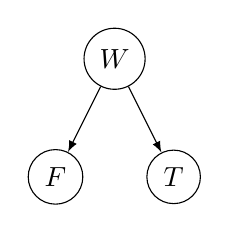
\begin{tikzpicture}[edge from parent/.style={draw,-latex}]
      \node[draw,circle] {$W$}
      child {node[draw,circle] {$F$}}
      child {node[draw,circle] {$T$}};
    \end{tikzpicture}
  \end{subfigure}%
  \begin{subfigure}{0.8\textwidth}
    \centering
    \begin{tabular}[t]{cc}
      \toprule
      $w$ & $\Pr(W = w)$ \\
      \midrule
      1 & 0.5 \\
      0 & 0.5 \\
      \bottomrule
    \end{tabular}
    \begin{tabular}[t]{ccc}
      \toprule
      $w$ & $f$ & $\Pr(F = f \mid W = w)$ \\
      \midrule
      1 & 1 & 0.6 \\
      1 & 0 & 0.4 \\
      0 & 1 & 0.1 \\
      0 & 0 & 0.9 \\
      \bottomrule
    \end{tabular}
    \begin{tabular}[t]{ccc}
      \toprule
      $w$ & $t$ & $\Pr(T = t \mid W = w)$ \\
      \midrule
      1 & $l$ & 0.2 \\
      1 & $m$ & 0.4 \\
      1 & $h$ & 0.4 \\
      0 & $l$ & 0.6 \\
      0 & $m$ & 0.3 \\
      0 & $h$ & 0.1 \\
      \bottomrule
    \end{tabular}
  \end{subfigure}
  \caption{An example Bayesian network with its CPTs}
  \label{fig:example_bn}
\end{figure}

In this section, we describe a way to encode Bayesian networks into WMC without
restricting oneself to factorable measures and thus having to add extra
variables to maintain literal independence. In line with the names of previous
encodings, we shall call this encoding \texttt{db21}. Recall that a Bayesian
network is a directed acyclic graph with random variables as vertices. Let
$\mathcal{V}$ denote the set of random variables. For any random variable $X \in
\mathcal{V}$, let $\im X$ denote its set of possible values and $\mathrm{pa}(X)$
the set of its parents. The full probability distribution is then equal to
$\prod_{X \in \mathcal{V}} \Pr(X \mid \mathrm{pa}(X))$. See
\cref{fig:example_bn} for an example Bayesian network which we will refer to
throughout this section. For this network, $\mathcal{V} = \{ W, F, T \}$,
$\mathrm{pa}(W) = \emptyset$, $\mathrm{pa}(F) = \mathrm{pa}(T) = \{ W \}$, $\im
W = \im F = \{0, 1 \}$, and $\im T = \{ l, m, h \}$.

\begin{definition}[Indicator variables]
  Let $X \in \mathcal{V}$ be a random variable. If $X$ is binary (i.e., $|\im X|
  = 2$), we can arbitrary identify one of the values as $1$ and the other one as
  $0$ (i.e, $\im X \cong \{ 0, 1 \}$). Then $X$ can be represented by a single
  \emph{indicator variable} $\lambda_{X=1}$. For notational simplicity, for any
  set $S$, we write $\lambda_{X=0} \in S$ or $S = \{ \lambda_{X=0}, \dots \}$ to
  mean $\lambda_{X=1} \not\in S$.

  On the other hand, if $X$ is not binary, we represent $X$ with $|\im X|$
  indicator variables, one for each value. We let
  \[
    \mathcal{E}(X) = \begin{cases}
      \{ \lambda_{X=1} \} & \text{if } |\im X| = 2 \\
      \{ \lambda_{X=x} \mid x \in \im X \} & \text{otherwise.}
    \end{cases}
  \]
  denote the set of indicator variables for $X$ and $\mathcal{E}^*(X) =
  \mathcal{E}(X) \cup \bigcup_{Y \in \mathrm{pa}(X)} \mathcal{E}(Y)$ denote the
  set of indicator variables for $X$ and its parents in the Bayesian network.
  Finally, let $U = \bigcup_{X \in \mathcal{V}} \mathcal{E}(X)$ denote the set
  of all indicator variables for all random variables in the Bayesian network.
\end{definition}

For the Bayesian network in \cref{fig:example_bn}, this gives us:
\begin{align*}
  \mathcal{E}(W) &= \{ \lambda_{W=1} \}, \\
  \mathcal{E}(F) &= \{ \lambda_{F=1} \}, \\
  \mathcal{E}(T) &= \{ \lambda_{T=l}, \lambda_{T=m}, \lambda_{T=h} \}, \\
  \mathcal{E}^*(W) &= \{ \lambda_{W=1} \}, \\
  \mathcal{E}^*(F) &= \{ \lambda_{F=1}, \lambda_{W=1} \}, \\
  \mathcal{E}^*(T) &= \{ \lambda_{T=l}, \lambda_{T=m}, \lambda_{T=h}, \lambda_{W=1} \}.
\end{align*}

\begin{algorithm}
  \caption{Encoding a Bayesian network as a function $2^U \to \mathbb{R}_{\ge
      0}$}
  \label{alg:encoding}
  \KwData{a Bayesian network with vertices $\mathcal{V}$ and probability
    distribution $\Pr$}
  \KwResult{a function $\phi\colon 2^U \to \mathbb{R}_{\ge 0}$}
  $\phi \gets 1$\;
  \For{$X \in \mathcal{V}$}{
    \textit{let} $\mathrm{pa}(X) = \{ Y_1, \dots, Y_n \}$\;
    $\mathrm{CPT}_X \gets 0$\;
    \eIf{$|\im X| = 2$}{
      \For{$(y_1, \dots, y_n) \in \prod_{i = 1}^n \im Y_i$}{
        $p_1 \gets \Pr(X = 1 \mid Y_1 = y_1, \dots, Y_n = y_n)$\;
        $p_0 \gets \Pr(X \ne 1 \mid Y_1 = y_1, \dots, Y_n = y_n)$\;
        $\mathrm{CPT}_X \gets \mathrm{CPT}_X + p_1[\lambda_{X=1}] \cdot
        \prod_{i=1}^n [\lambda_{Y_i=y_i}] + p_0 \overline{[\lambda_{X=1}]} \cdot
        \prod_{i=1}^n [\lambda_{Y_i=y_i}]$\;
      }
    }{
      \textit{let} $\im X = \{ x_1, \dots, x_m \}$\;
      \For{$x \in \im X$ {\rm \textbf{and}} $(y_1, \dots, y_n) \in \prod_{i =
          1}^n \im Y_i$}{
        $p_x \gets \Pr(X = x \mid Y_1 = y_1, \dots, Y_n = y_n)$\;
        $\mathrm{CPT}_X \gets \mathrm{CPT}_X + p_x[\lambda_{X=x}] \cdot
        \prod_{i=1}^n [\lambda_{Y_i=y_i}] + \overline{[\lambda_{X=1}]} \cdot
        \prod_{i=1}^n [\lambda_{Y_i=y_i}]$\;
      }
      $\mathrm{CPT}_X \gets \mathrm{CPT}_X \cdot \left( \sum_{i=1}^m [\lambda_{X
          = x_i}] \right) \cdot \prod_{i=1}^m \prod_{j=i+1}^m
      (\overline{[\lambda_{X = x_i}]} + \overline{[\lambda_{X = x_j}]})$\;
    }
    $\phi \gets \phi \cdot \mathrm{CPT}_X$\;
  }
  \Return{$\phi$}\;
\end{algorithm}

\Cref{alg:encoding} shows how a Bayesian network with vertices $\mathcal{V}$
can be represented as a weight function $\phi\colon 2^U \to \mathbb{R}_{\ge 0}$.
The algorithm begins with the unit function and multiplies it by
$\mathrm{CPT}_X\colon 2^{\mathcal{E}^*(X)} \to \mathbb{R}_{\ge 0}$ for each
random variable $X \in \mathcal{V}$. We call each such function a
\emph{conditional weight function} as it represents a conditional probability
distribution. However, the distinction is primarily a semantic one: a function
$2^{\{a, b\}} \to \mathbb{R}_{\ge 0}$ can represent $\Pr(a \mid b)$, $\Pr(b \mid
a)$, or something else entirely.

For a binary random variable $X$, $\mathrm{CPT}_X$ is simply a sum of smaller
functions, one for each row of the CPT. If $X$ has more than two values, we also
multiply $\mathrm{CPT}_X$ by some `clause' functions that restrict the value of
$\phi(T)$ to zero whenever $|\mathcal{E}(X) \cap T| \ne 1$. For the Bayesian
network in \cref{fig:example_bn}, we get:
\begin{align*}
  \mathrm{CPT_W} &= 0.5[\lambda_{W=1}]+0.5\overline{[\lambda_{W=1}]} = 0.5 \cdot 1, \\
  \mathrm{CPT_F} &= 0.6[\lambda_{F=1}] \cdot [\lambda_{W=1}] + 0.4[\lambda_{F=0}] \cdot [\lambda_{W=1}] + 0.1[\lambda_{F=1}] \cdot [\lambda_{W=0}] + 0.9[\lambda_{F=0}] \cdot [\lambda_{W=0}] \\
    &= 0.6[\lambda_{F=1}] \cdot [\lambda_{W=1}] + 0.4\overline{[\lambda_{F=1}]} \cdot [\lambda_{W=1}] + 0.1[\lambda_{F=1}] \cdot \overline{[\lambda_{W=1}]} + 0.9\overline{[\lambda_{F=1}]} \cdot \overline{[\lambda_{W=1}]}, \\
  \mathrm{CPT_T} &= ([\lambda_{T=l}] + [\lambda_{T=m}] + [\lambda_{T=h}]) \cdot (\overline{[\lambda_{T=l}]} + \overline{[\lambda_{T=m}]}) \cdot (\overline{[\lambda_{T=l}]} + \overline{[\lambda_{T=h}]}) \cdot (\overline{[\lambda_{T=m}]} + \overline{[\lambda_{T=h}]}) \cdot (\dots).
\end{align*}

\subsection{Proof of Correctness}

\Cref{alg:encoding} produces a function with a Boolean algebra as its domain.
This function can be represented by an ADD. The core of ADDMC works by taking an
ADD $\psi\colon 2^{U} \to \mathbb{R}_{\ge 0}$ (expressed as a product of smaller
ADDs) and returning $(\exists_U\psi)(\emptyset)$
\cite{DBLP:conf/aaai/DudekPV20}. In this section, we prove that the function
$\phi$ produced by \cref{alg:encoding} can be used by ADDMC to correctly compute
any marginal probability of the Bayesian network that was encoded as
$\phi$.\footnote{It can just as well compute any probability expressed using the
random variables in $\mathcal{V}$, but we focus mostly on marginal probabilities
in our experiments.} First, \cref{lemma:cpt} shows that any conditional weight function
produces the right answer when given an appropriate encoding of
variable-value assignments for a conditional probability in the Bayesian
network. Then, \cref{lemma:full_distribution} shows that $\phi$ represents the
full probability distribution of the Bayesian network, i.e., it gives the right
probabilities for the right inputs and zero otherwise. We end with
\cref{thm:correctness} that shows how $\phi$ can be combined with an encoding of
a single variable-value assignment so that ADDMC would compute its marginal
probability.

\begin{lemma} \label{lemma:cpt}
  Let $X \in \mathcal{V}$ be a random variable with parents $\mathrm{pa}(X) = \{ Y_1,
  \dots, Y_n \}$. Then $\mathrm{CPT}_X\colon 2^{\mathcal{E}^*(X)} \to
  \mathbb{R}_{\ge 0}$ is such that for any $x \in \im X$ and $(y_1, \dots, y_n)
  \in \prod_{i=1}^n \im Y_i$,
  \[
    \mathrm{CPT}_X (\{ \lambda_{X=x} \} \cup \{ \lambda_{Y_i=y_i} \mid i = 1,
    \dots, n \}) = \Pr(X = x \mid Y_1 = y_1, \dots, Y_n = y_n).
  \]
\end{lemma}
\begin{proof}
  Let $T = \{ \lambda_{X=x} \} \cup \{ \lambda_{Y_i=y_i} \mid i = 1, \dots, n
  \}$. If $X$ is binary, then $\mathrm{CPT}_X$ is a sum of $2\prod_{i=1}^n |\im
  Y_i|$ terms, one for each possible assignment of values to variables $X, Y_1,
  \dots, Y_n$. Exactly one of these terms is nonzero when applied to $T$, and
  it is equal to $\Pr(X = x \mid Y_1 = y_1, \dots, Y_n = y_n)$ by definition.

  If $X$ is not binary, then $\left( \sum_{i=1}^m [\lambda_{X = x_i}]
  \right)(T) = 1$, and $\left( \prod_{i=1}^m \prod_{j=i+1}^m
    (\overline{[\lambda_{X = x_i}]} + \overline{[\lambda_{X = x_j}]})
  \right)(T) = 1$, so $\mathrm{CPT}_X(T) = \Pr(X = x \mid Y_1 = y_1,
  \dots, Y_n = y_n)$ by a similar argument as before.
\end{proof}

\begin{proposition} \label{lemma:full_distribution}
  Let $\mathcal{V} = \{X_1, \dots, X_n\}$. Then
  \[
    \phi(T) =
    \begin{cases}
      \Pr(X_1 = x_1, \dots, X_n = x_n) & \text{if } T = \{ \lambda_{X_i=x_i}
      \mid i = 1, \dots, n \} \text{ for some } (x_1, \dots, x_n) \in
      \prod_{i=1}^n \im X_i \\
      0 & \text{otherwise,}
    \end{cases}
  \]
  for all $T \in 2^U$.
\end{proposition}
\begin{proof}
  If $T = \{ \lambda_{X=v_X} \mid X \in \mathcal{V} \}$ for some $(v_X)_{X
    \in \mathcal{V}} \in \prod_{X \in \mathcal{V}} \im X$, then
  \[
    \phi(T) = \prod_{X \in \mathcal{V}} \Pr \left( X=v_X \;\middle|\;
      \bigwedge_{Y \in \mathrm{pa}(X)} Y=v_Y \right) = \Pr \left( \bigwedge_{X
        \in \mathcal{V}} X=v_X \right)
  \]
  by \cref{lemma:cpt} and the definition of a Bayesian network. Otherwise there
  must be some non-binary random variable $X \in \mathcal{V}$ such that
  $|\mathcal{E}(X) \cap T| \ne 1$. If $\mathcal{E}(X) \cap T = \emptyset$, then
  $\left( \sum_{i=1}^m [\lambda_{X = x_i}] \right)(T) = 0$, and so
  $\mathrm{CPT}_X(T) = 0$, and $\phi(T) = 0$. If $|\mathcal{E}(X) \cap T| > 1$,
  then we must have two different values $x_1, x_2 \in \im X$ such that
  $\{\lambda_{X=x_1}, \lambda_{X=x_2} \} \subseteq T$ which means that
  $(\overline{[\lambda_{X=x_1}]} + \overline{[\lambda_{X=x_2}]})(T) = 0$, and
  so, again, $\mathrm{CPT}_X(T) = 0$, and $\phi(T) = 0$.
\end{proof}

\begin{theorem} \label{thm:correctness}
  For any $X \in \mathcal{V}$ and $x \in \im X$, $(\exists_U(\phi \cdot
  [\lambda_{X=x}]))(\emptyset) = \Pr(X = x)$.
\end{theorem}
\begin{proof}
  Let $\mathcal{V} = \{ X, Y_1, \dots, Y_n \}$. Then
  \begin{align*}
    (\exists_U (\phi \cdot [\lambda_{X=x}]))(\emptyset) &= \sum_{T \in 2^U} (\phi \cdot [\lambda_{X=x}])(T) = \sum_{\lambda_{X=x} \in T \in 2^U} \phi(T) = \sum_{\lambda_{X=x} \in T \in 2^U} \left( \prod_{Y \in \mathcal{V}} \mathrm{CPT}_Y \right)(T) \\
    &= \sum_{(y_1, \dots, y_n) \in \prod_{i=1}^n \im Y_i} \Pr(X = x, Y_1 = y_1, \dots, Y_n = y_n) = \Pr(X = x)
  \end{align*}
  by the following arguments:
  \begin{itemize}
  \item the proof of Theorem~1 in the ADDMC paper \cite{DBLP:conf/aaai/DudekPV20};
  \item if $\lambda_{X=x} \not\in T \in 2^U$, then $(\phi \cdot
    [\lambda_{X=x}])(T) = \phi(T) \cdot [\lambda_{X=x}](T \cap \{
    \lambda_{X=x} \}) = \phi(T) \cdot 0 = 0$;
  \item \cref{lemma:full_distribution};
  \item marginalisation of a probability distribution.
  \end{itemize}
\end{proof}
\todo[inline]{Need to make the proof nicer.}

\subsection{Textual Representation} \label{sec:textual_representation}

\Cref{alg:encoding} encodes a Bayesian network into a function on a Boolean
algebra, but how does it relate to the standard interpretation of a WMC encoding
as a formula in conjunctive normal form (CNF) together with a collection of
weights? The factors of $\phi$ that restrict the values of indicator variables
for non-binary random variables are already expressed as a product of sums of
0/1-valued functions, i.e., a kind of CNF. Disregarding these functions, each
conditional weight function $\mathrm{CPT}_X$ is represented by a sum with a term
for every subset of $\mathcal{E}^*(X)$. To encode these terms, we introduce
\emph{extended weight clauses} to the WMC format used by Cachet
\cite{DBLP:conf/sat/SangBBKP04}. For instance, here is a representation of the
Bayesian network from \cref{fig:example_bn}:
\[
  \begin{array}{lrrll}
    \lambda\sb{T=l} &\lambda\sb{T=m} &\lambda\sb{T=h} & &0 \\
                    &-\lambda\sb{T=l} &-\lambda\sb{T=m} & &0 \\
                    &-\lambda\sb{T=l} &-\lambda\sb{T=h} & &0 \\
                    &-\lambda\sb{T=m} &-\lambda\sb{T=h} & &0 \\
    w &\lambda\sb{W=1} & &0.5 &0.5 \\
    w &\lambda\sb{F=1} &\lambda\sb{W=1} &0.6 &0.4 \\
    w &\lambda\sb{F=1} &-\lambda\sb{W=1} &0.1 &0.9 \\
    w &\lambda\sb{T=l} &\lambda\sb{W=1} &0.2 &1 \\
    w &\lambda\sb{T=m} &\lambda\sb{W=1} &0.4 &1 \\
    w &\lambda\sb{T=h} &\lambda\sb{W=1} &0.4 &1 \\
    w &\lambda\sb{T=l} &-\lambda\sb{W=1} &0.6 &1 \\
    w &\lambda\sb{T=m} &-\lambda\sb{W=1} &0.3 &1 \\
    w &\lambda\sb{T=h} &-\lambda\sb{W=1} &0.1 &1
  \end{array}
\]
where each indicator variable is eventually replaced with a unique positive
integer. Each line prefixed with a $w$ can be split into four parts: the `main'
variable (always not negated), conditions (possibly none), and two weights. For
example, the line
\[
  \begin{array}{lrrll}
    w &\lambda\sb{T=m} &-\lambda\sb{W=1} &0.3 &1
  \end{array}
\]
encodes the function $0.3[\lambda_{T=m}] \cdot \overline{[\lambda_{W=1}]} +
1\overline{[\lambda_{T=m}]} \cdot \overline{[\lambda_{W=1}]}$ and can be
interpreted as defining two conditional weights: $\nu(T = m \mid W = 0) = 0.3$,
and $\nu(T \ne m \mid W = 0) = 1$, the former of which corresponds to a row in
the CPT of $T$ while the latter is artificially added as part of the encoding.
In our encoding of Bayesian networks, it is always the case that, in each weight
clause, either both weights sum to one, or the second weight is equal to one.
Finally, note that (without any additional restrictions), the measure induced by
these weight functions is not probabilistic (i.e., $\mu(\top)$ may not be equal
to one).

\subsection{Changes to ADDMC}

ADDMC constructs the \emph{Gaifman graph} \cite{gaifman1982local} of the input
CNF formula as an aid for the algorithm's heuristics. This graph has as vertices
the variables of the formula, and there is an edge between two variables $u$ and
$v$ if there is a clause in the formula that contains both $u$ and $v$. We
extend this definition to functions on Boolean algebras, i.e., the factors of
$\phi$. For any pair of distinct variables $u, v \in U$, we draw an edge between
them in the Gaifman graph if there is a function $\alpha\colon 2^X \to
\mathbb{R}_{\ge 0}$ that is a factor of $\phi$ such that $u \in X$ and $v \in
X$. For instance, a factor such as $\mathrm{CPT}_X$ will enable edges between
all distinct pairs of variables in $\mathcal{E}^*(X)$.

Even though the function $\phi$ produced by \cref{alg:encoding} is constructed
to have $2^U$ as its domain, sometimes the domain is effectively reduced to
$2^V$ for some $V \subset U$ by the ADD manipulation algorithms that optimise
the ADD representation of a function. For a simple example, consider $\alpha:
2^{\{a\}} \to \mathbb{R}_{\ge 0}$ defined as $\alpha(\{a\}) = \alpha(\emptyset)
= 0.5$. Then $\alpha$ can be reduced to $\alpha'\colon 2^{\emptyset} \to
\mathbb{R}_{\ge 0}$ defined as $\alpha'(\emptyset) = 0.5$. To compensate for
these reductions, for the original WMC format with a weight function $w\colon U
\cup \{ \neg u \mid u \in U \} \to \mathbb{R}_{\ge 0}$, ADDMC would multiply its
computed answer by $\prod_{u \in U \setminus V} w(u) + w(\neg u)$. With the new
WMC format, we instead multiply the answer by $2^{|U \setminus V|}$. Each
`excluded' variable $u \in U \setminus V$ satisfies two properties:
all weights associated with $u$ are equal to $0.5$ (otherwise the corresponding
CPT would depend on $u$, and $u$ would not be excluded), and all other CPTs are
independent of $u$ (or they may have a trivial dependence, where the probability
stays the same if $u$ is replaced with its complement).
Thus, the CPT that corresponds to $u$ still multiplies every model by $0.5$, but
the number of models being considered by the ADDMC is halved. To correct for
this, we multiply the final answer by two for every $u \in U \setminus V$.

\section{Experimental Comparison} \label{sec:experiments}

\begin{figure}
  \centering
  \begin{minipage}{0.59\textwidth}
    \centering
    % Created by tikzDevice version 0.12.3 on 2020-08-01 17:20:52
% !TEX encoding = UTF-8 Unicode
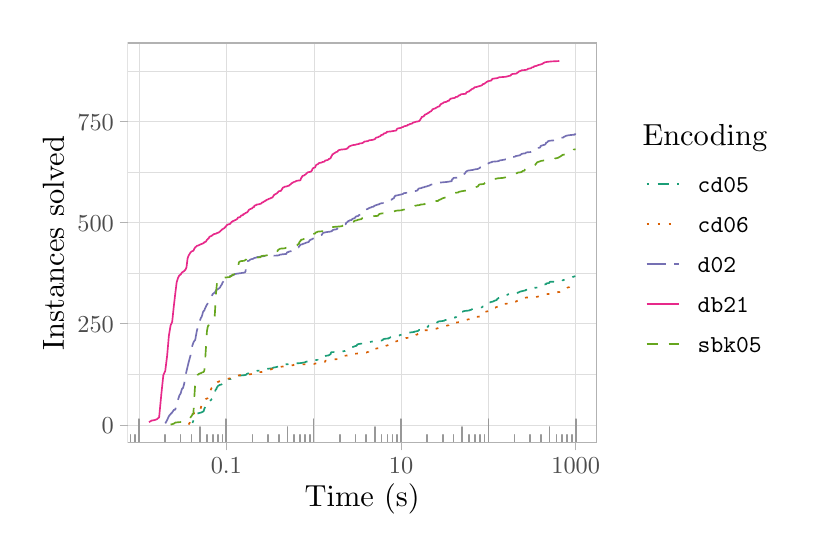
\begin{tikzpicture}[x=1pt,y=1pt]
\definecolor{fillColor}{RGB}{255,255,255}
\path[use as bounding box,fill=fillColor,fill opacity=0.00] (0,0) rectangle (278.24,180.67);
\begin{scope}
\path[clip] (  0.00,  0.00) rectangle (278.24,180.67);
\definecolor{drawColor}{RGB}{255,255,255}
\definecolor{fillColor}{RGB}{255,255,255}

\path[draw=drawColor,line width= 0.6pt,line join=round,line cap=round,fill=fillColor] (  0.00,  0.00) rectangle (278.24,180.68);
\end{scope}
\begin{scope}
\path[clip] ( 36.11, 30.69) rectangle (205.68,175.17);
\definecolor{fillColor}{RGB}{255,255,255}

\path[fill=fillColor] ( 36.11, 30.69) rectangle (205.68,175.17);
\definecolor{drawColor}{gray}{0.87}

\path[draw=drawColor,line width= 0.1pt,line join=round] ( 36.11, 55.37) --
	(205.68, 55.37);

\path[draw=drawColor,line width= 0.1pt,line join=round] ( 36.11, 91.90) --
	(205.68, 91.90);

\path[draw=drawColor,line width= 0.1pt,line join=round] ( 36.11,128.43) --
	(205.68,128.43);

\path[draw=drawColor,line width= 0.1pt,line join=round] ( 36.11,164.95) --
	(205.68,164.95);

\path[draw=drawColor,line width= 0.1pt,line join=round] ( 40.22, 30.69) --
	( 40.22,175.17);

\path[draw=drawColor,line width= 0.1pt,line join=round] (103.34, 30.69) --
	(103.34,175.17);

\path[draw=drawColor,line width= 0.1pt,line join=round] (166.47, 30.69) --
	(166.47,175.17);

\path[draw=drawColor,line width= 0.3pt,line join=round] ( 36.11, 37.11) --
	(205.68, 37.11);

\path[draw=drawColor,line width= 0.3pt,line join=round] ( 36.11, 73.64) --
	(205.68, 73.64);

\path[draw=drawColor,line width= 0.3pt,line join=round] ( 36.11,110.16) --
	(205.68,110.16);

\path[draw=drawColor,line width= 0.3pt,line join=round] ( 36.11,146.69) --
	(205.68,146.69);

\path[draw=drawColor,line width= 0.3pt,line join=round] ( 71.78, 30.69) --
	( 71.78,175.17);

\path[draw=drawColor,line width= 0.3pt,line join=round] (134.91, 30.69) --
	(134.91,175.17);

\path[draw=drawColor,line width= 0.3pt,line join=round] (198.03, 30.69) --
	(198.03,175.17);
\definecolor{drawColor}{RGB}{27,158,119}

\path[draw=drawColor,line width= 0.6pt,dash pattern=on 1pt off 3pt on 4pt off 3pt ,line join=round] ( 59.56, 37.84) --
	( 59.89, 38.71) --
	( 60.22, 39.74) --
	( 60.53, 40.47) --
	( 60.84, 40.91) --
	( 61.14, 41.20) --
	( 62.82, 41.64) --
	( 63.59, 42.08) --
	( 63.84, 42.95) --
	( 64.08, 43.54) --
	( 64.32, 44.41) --
	( 64.55, 44.85) --
	( 64.78, 45.14) --
	( 65.01, 45.29) --
	( 65.23, 45.44) --
	( 65.45, 45.58) --
	( 65.88, 45.87) --
	( 66.09, 46.02) --
	( 66.29, 46.17) --
	( 66.50, 46.46) --
	( 66.89, 46.75) --
	( 67.09, 47.34) --
	( 67.28, 47.63) --
	( 67.47, 48.07) --
	( 67.66, 48.80) --
	( 67.84, 49.67) --
	( 68.02, 49.97) --
	( 68.20, 50.11) --
	( 68.38, 50.70) --
	( 68.55, 50.84) --
	( 68.73, 51.13) --
	( 68.90, 51.28) --
	( 69.39, 51.57) --
	( 70.03, 51.72) --
	( 70.19, 51.86) --
	( 70.34, 52.01) --
	( 70.49, 52.16) --
	( 70.64, 52.60) --
	( 70.79, 52.74) --
	( 70.94, 53.03) --
	( 71.08, 53.18) --
	( 71.37, 53.33) --
	( 71.92, 53.47) --
	( 72.32, 53.62) --
	( 73.46, 53.76) --
	( 73.58, 53.91) --
	( 73.82, 54.20) --
	( 74.73, 54.35) --
	( 74.84, 54.49) --
	( 75.38, 54.64) --
	( 76.00, 54.79) --
	( 76.20, 54.93) --
	( 78.14, 55.08) --
	( 78.89, 55.23) --
	( 79.06, 55.37) --
	( 79.14, 55.52) --
	( 79.38, 55.66) --
	( 79.84, 55.81) --
	( 80.80, 55.96) --
	( 81.01, 56.10) --
	( 81.56, 56.25) --
	( 82.15, 56.39) --
	( 82.40, 56.54) --
	( 82.90, 56.69) --
	( 84.51, 56.83) --
	( 85.55, 56.98) --
	( 85.60, 57.12) --
	( 86.14, 57.27) --
	( 86.75, 57.42) --
	( 88.27, 57.56) --
	( 88.56, 57.71) --
	( 88.92, 57.86) --
	( 89.68, 58.00) --
	( 90.33, 58.15) --
	( 91.26, 58.29) --
	( 92.25, 58.44) --
	( 92.67, 58.59) --
	( 92.82, 58.73) --
	( 92.88, 58.88) --
	( 93.23, 59.02) --
	( 95.54, 59.17) --
	( 95.78, 59.32) --
	( 98.51, 59.46) --
	( 99.60, 59.61) --
	(100.18, 59.75) --
	(100.44, 59.90) --
	(100.97, 60.05) --
	(102.70, 60.19) --
	(102.77, 60.34) --
	(103.18, 60.49) --
	(104.73, 60.63) --
	(104.84, 60.78) --
	(104.86, 60.92) --
	(105.61, 61.07) --
	(105.71, 61.22) --
	(105.76, 61.36) --
	(106.49, 61.65) --
	(106.71, 61.80) --
	(107.11, 61.95) --
	(107.66, 62.09) --
	(108.70, 62.24) --
	(108.94, 62.38) --
	(109.14, 62.53) --
	(109.44, 62.68) --
	(109.53, 62.82) --
	(109.55, 62.97) --
	(109.56, 63.12) --
	(109.61, 63.26) --
	(109.79, 63.41) --
	(113.34, 63.55) --
	(113.86, 63.70) --
	(114.65, 63.85) --
	(114.85, 63.99) --
	(114.96, 64.14) --
	(115.67, 64.28) --
	(115.88, 64.43) --
	(115.93, 64.58) --
	(116.05, 64.72) --
	(116.59, 64.87) --
	(116.80, 65.01) --
	(117.01, 65.16) --
	(117.54, 65.31) --
	(117.99, 65.45) --
	(118.33, 65.60) --
	(118.91, 65.75) --
	(118.95, 65.89) --
	(119.00, 66.04) --
	(119.07, 66.18) --
	(119.49, 66.33) --
	(120.39, 66.48) --
	(122.58, 66.62) --
	(123.52, 66.77) --
	(123.65, 66.91) --
	(123.88, 67.06) --
	(124.05, 67.21) --
	(125.63, 67.35) --
	(125.97, 67.50) --
	(127.90, 67.64) --
	(128.29, 67.79) --
	(128.40, 67.94) --
	(128.51, 68.08) --
	(128.93, 68.23) --
	(130.47, 68.38) --
	(130.56, 68.52) --
	(130.91, 68.67) --
	(131.06, 68.81) --
	(132.13, 68.96) --
	(132.68, 69.11) --
	(132.88, 69.25) --
	(134.33, 69.40) --
	(134.38, 69.54) --
	(134.92, 69.69) --
	(135.51, 69.84) --
	(135.83, 69.98) --
	(136.08, 70.13) --
	(136.75, 70.27) --
	(137.17, 70.42) --
	(138.61, 70.57) --
	(139.62, 70.71) --
	(139.84, 70.86) --
	(140.77, 71.01) --
	(141.17, 71.15) --
	(141.26, 71.30) --
	(141.42, 71.44) --
	(143.11, 71.59) --
	(143.19, 71.74) --
	(143.46, 71.88) --
	(144.14, 72.03) --
	(144.34, 72.17) --
	(144.37, 72.32) --
	(144.48, 72.47) --
	(144.58, 72.61) --
	(144.79, 72.76) --
	(144.81, 72.90) --
	(144.95, 73.05) --
	(145.24, 73.20) --
	(145.47, 73.34) --
	(145.92, 73.49) --
	(147.23, 73.64) --
	(147.44, 73.78) --
	(147.46, 73.93) --
	(147.72, 74.07) --
	(148.22, 74.22) --
	(148.27, 74.37) --
	(148.30, 74.51) --
	(149.81, 74.66) --
	(150.57, 74.80) --
	(150.66, 74.95) --
	(151.33, 75.10) --
	(151.51, 75.24) --
	(151.72, 75.39) --
	(152.00, 75.53) --
	(152.11, 75.68) --
	(152.77, 75.83) --
	(154.61, 75.97) --
	(154.83, 76.12) --
	(154.90, 76.27) --
	(154.95, 76.41) --
	(155.00, 76.56) --
	(155.20, 76.70) --
	(155.26, 76.85) --
	(155.28, 77.00) --
	(155.81, 77.14) --
	(155.83, 77.29) --
	(155.95, 77.43) --
	(156.19, 77.58) --
	(156.23, 77.73) --
	(156.33, 77.87) --
	(157.14, 78.02) --
	(157.39, 78.16) --
	(158.01, 78.31) --
	(159.50, 78.46) --
	(159.73, 78.60) --
	(160.29, 78.75) --
	(160.47, 78.90) --
	(161.11, 79.04) --
	(161.73, 79.19) --
	(162.65, 79.33) --
	(163.23, 79.48) --
	(164.16, 79.63) --
	(164.29, 79.77) --
	(164.53, 79.92) --
	(165.13, 80.06) --
	(165.72, 80.21) --
	(165.75, 80.36) --
	(165.77, 80.50) --
	(166.15, 80.65) --
	(166.22, 80.79) --
	(166.27, 80.94) --
	(166.35, 81.09) --
	(166.35, 81.23) --
	(167.05, 81.38) --
	(167.35, 81.53) --
	(168.04, 81.67) --
	(168.37, 81.82) --
	(168.61, 81.96) --
	(169.05, 82.11) --
	(169.51, 82.26) --
	(169.52, 82.40) --
	(169.62, 82.55) --
	(169.80, 82.69) --
	(169.96, 82.84) --
	(170.15, 82.99) --
	(170.56, 83.13) --
	(170.65, 83.28) --
	(170.96, 83.42) --
	(171.94, 83.57) --
	(172.12, 83.72) --
	(172.36, 83.86) --
	(172.47, 84.01) --
	(173.42, 84.16) --
	(173.44, 84.30) --
	(175.96, 84.45) --
	(176.63, 84.59) --
	(176.97, 84.74) --
	(176.99, 84.89) --
	(177.55, 85.03) --
	(177.57, 85.18) --
	(178.08, 85.32) --
	(178.68, 85.47) --
	(179.32, 85.62) --
	(179.91, 85.76) --
	(180.02, 85.91) --
	(181.06, 86.05) --
	(181.14, 86.20) --
	(181.21, 86.35) --
	(182.87, 86.49) --
	(182.94, 86.64) --
	(184.41, 86.79) --
	(184.74, 86.93) --
	(184.93, 87.08) --
	(185.23, 87.22) --
	(185.27, 87.37) --
	(185.96, 87.52) --
	(186.07, 87.66) --
	(186.19, 87.81) --
	(187.31, 87.95) --
	(187.35, 88.10) --
	(187.37, 88.25) --
	(188.44, 88.39) --
	(188.53, 88.54) --
	(188.55, 88.68) --
	(188.68, 88.83) --
	(192.45, 88.98) --
	(193.20, 89.12) --
	(193.28, 89.27) --
	(193.38, 89.42) --
	(193.89, 89.56) --
	(194.14, 89.71) --
	(194.52, 89.85) --
	(195.52, 90.00) --
	(195.91, 90.15) --
	(196.52, 90.29) --
	(196.72, 90.44) --
	(196.95, 90.58) --
	(197.43, 90.73) --
	(197.91, 90.88);
\definecolor{drawColor}{RGB}{217,95,2}

\path[draw=drawColor,line width= 0.6pt,dash pattern=on 1pt off 3pt ,line join=round] ( 58.16, 37.25) --
	( 58.52, 37.84) --
	( 58.88, 39.59) --
	( 59.22, 40.47) --
	( 59.56, 41.05) --
	( 60.22, 41.34) --
	( 61.14, 41.49) --
	( 61.43, 41.78) --
	( 62.01, 41.93) --
	( 62.28, 42.08) --
	( 62.55, 43.24) --
	( 62.82, 44.27) --
	( 63.08, 44.85) --
	( 63.34, 45.44) --
	( 63.84, 45.87) --
	( 64.08, 46.02) --
	( 64.32, 46.46) --
	( 65.01, 46.75) --
	( 65.23, 46.90) --
	( 65.45, 47.34) --
	( 65.67, 47.77) --
	( 65.88, 48.65) --
	( 66.09, 49.53) --
	( 66.29, 50.11) --
	( 66.50, 50.55) --
	( 66.70, 50.84) --
	( 66.89, 51.43) --
	( 67.09, 51.57) --
	( 67.28, 51.72) --
	( 67.47, 51.86) --
	( 67.84, 52.01) --
	( 68.02, 52.16) --
	( 68.38, 52.30) --
	( 68.55, 52.60) --
	( 69.06, 52.74) --
	( 69.23, 52.89) --
	( 69.56, 53.03) --
	( 69.87, 53.18) --
	( 70.19, 53.33) --
	( 70.94, 53.47) --
	( 71.65, 53.62) --
	( 71.78, 53.76) --
	( 72.97, 53.91) --
	( 73.46, 54.06) --
	( 73.82, 54.20) --
	( 74.28, 54.49) --
	( 74.84, 54.64) --
	( 74.95, 54.79) --
	( 75.49, 54.93) --
	( 76.59, 55.08) --
	( 79.22, 55.23) --
	( 79.84, 55.37) --
	( 81.01, 55.52) --
	( 81.08, 55.66) --
	( 81.15, 55.81) --
	( 82.34, 55.96) --
	( 82.72, 56.10) --
	( 84.56, 56.25) --
	( 85.50, 56.39) --
	( 86.19, 56.54) --
	( 86.47, 56.69) --
	( 87.11, 56.83) --
	( 87.34, 56.98) --
	( 87.73, 57.12) --
	( 88.11, 57.27) --
	( 88.44, 57.42) --
	( 88.72, 57.56) --
	( 90.61, 57.86) --
	( 90.85, 58.00) --
	( 91.55, 58.15) --
	( 92.76, 58.29) --
	( 93.82, 58.44) --
	( 94.85, 58.59) --
	( 96.09, 58.73) --
	( 96.16, 58.88) --
	(100.27, 59.02) --
	(103.56, 59.17) --
	(103.99, 59.32) --
	(104.98, 59.46) --
	(105.40, 59.61) --
	(106.51, 59.75) --
	(107.46, 59.90) --
	(107.47, 60.05) --
	(107.50, 60.19) --
	(107.71, 60.34) --
	(108.64, 60.49) --
	(109.52, 60.63) --
	(110.62, 60.78) --
	(112.04, 60.92) --
	(112.14, 61.07) --
	(112.60, 61.22) --
	(112.83, 61.36) --
	(113.18, 61.51) --
	(113.48, 61.65) --
	(113.88, 61.80) --
	(114.05, 61.95) --
	(114.28, 62.09) --
	(115.62, 62.24) --
	(117.04, 62.38) --
	(117.14, 62.53) --
	(117.17, 62.68) --
	(117.61, 62.82) --
	(120.08, 62.97) --
	(120.83, 63.12) --
	(122.39, 63.26) --
	(122.72, 63.41) --
	(123.16, 63.55) --
	(123.21, 63.70) --
	(123.36, 63.85) --
	(123.36, 63.99) --
	(123.39, 64.14) --
	(123.45, 64.28) --
	(123.90, 64.43) --
	(125.26, 64.58) --
	(126.04, 64.72) --
	(126.78, 64.87) --
	(126.86, 65.01) --
	(126.88, 65.16) --
	(127.97, 65.31) --
	(128.41, 65.45) --
	(129.17, 65.60) --
	(129.56, 65.75) --
	(130.06, 65.89) --
	(130.38, 66.04) --
	(130.54, 66.18) --
	(130.85, 66.33) --
	(130.89, 66.48) --
	(131.15, 66.62) --
	(131.28, 66.77) --
	(132.02, 66.91) --
	(132.22, 67.06) --
	(132.44, 67.21) --
	(133.43, 67.35) --
	(133.58, 67.50) --
	(134.96, 67.64) --
	(135.14, 67.79) --
	(135.24, 67.94) --
	(135.48, 68.08) --
	(135.83, 68.23) --
	(136.36, 68.38) --
	(136.68, 68.52) --
	(138.14, 68.67) --
	(138.61, 68.81) --
	(139.38, 68.96) --
	(139.38, 69.11) --
	(139.57, 69.25) --
	(139.89, 69.40) --
	(140.07, 69.54) --
	(140.31, 69.69) --
	(140.91, 69.84) --
	(140.91, 69.98) --
	(141.45, 70.13) --
	(141.90, 70.27) --
	(142.10, 70.42) --
	(142.92, 70.57) --
	(143.07, 70.71) --
	(143.09, 70.86) --
	(143.28, 71.01) --
	(143.30, 71.15) --
	(143.55, 71.30) --
	(145.67, 71.44) --
	(145.79, 71.59) --
	(146.91, 71.74) --
	(147.53, 71.88) --
	(148.12, 72.03) --
	(148.43, 72.17) --
	(149.21, 72.32) --
	(149.80, 72.47) --
	(149.98, 72.61) --
	(150.56, 72.76) --
	(150.83, 72.90) --
	(151.81, 73.05) --
	(152.13, 73.20) --
	(152.20, 73.34) --
	(152.27, 73.49) --
	(152.29, 73.64) --
	(152.51, 73.78) --
	(153.79, 73.93) --
	(154.57, 74.07) --
	(155.62, 74.22) --
	(156.39, 74.37) --
	(156.92, 74.51) --
	(157.40, 74.66) --
	(157.72, 74.80) --
	(158.16, 74.95) --
	(158.71, 75.10) --
	(159.02, 75.24) --
	(160.09, 75.39) --
	(161.11, 75.53) --
	(161.61, 75.68) --
	(161.61, 75.83) --
	(161.64, 75.97) --
	(161.96, 76.12) --
	(163.07, 76.27) --
	(163.87, 76.41) --
	(164.09, 76.56) --
	(164.16, 76.70) --
	(164.19, 76.85) --
	(164.19, 77.00) --
	(164.27, 77.14) --
	(164.36, 77.29) --
	(164.37, 77.43) --
	(164.74, 77.58) --
	(164.89, 77.73) --
	(165.08, 77.87) --
	(165.27, 78.02) --
	(166.19, 78.16) --
	(166.53, 78.31) --
	(167.14, 78.46) --
	(167.22, 78.60) --
	(167.32, 78.75) --
	(167.41, 78.90) --
	(167.47, 79.04) --
	(167.60, 79.19) --
	(168.37, 79.33) --
	(168.97, 79.48) --
	(169.19, 79.63) --
	(169.60, 79.77) --
	(169.95, 79.92) --
	(170.05, 80.06) --
	(170.07, 80.21) --
	(170.29, 80.36) --
	(170.32, 80.50) --
	(171.11, 80.65) --
	(172.05, 80.79) --
	(173.03, 80.94) --
	(174.96, 81.09) --
	(175.34, 81.23) --
	(175.36, 81.38) --
	(175.59, 81.53) --
	(176.49, 81.67) --
	(176.54, 81.82) --
	(176.94, 81.96) --
	(177.77, 82.11) --
	(178.02, 82.26) --
	(178.10, 82.40) --
	(178.99, 82.55) --
	(179.08, 82.69) --
	(179.24, 82.84) --
	(179.51, 82.99) --
	(179.99, 83.13) --
	(183.14, 83.28) --
	(183.99, 83.42) --
	(184.68, 83.57) --
	(185.02, 83.72) --
	(185.75, 83.86) --
	(186.49, 84.01) --
	(186.80, 84.16) --
	(187.12, 84.30) --
	(188.18, 84.45) --
	(190.60, 84.59) --
	(190.74, 84.74) --
	(190.94, 84.89) --
	(191.10, 85.03) --
	(192.25, 85.18) --
	(192.34, 85.32) --
	(192.58, 85.47) --
	(192.67, 85.62) --
	(193.26, 85.76) --
	(193.55, 85.91) --
	(194.02, 86.05) --
	(194.49, 86.20) --
	(194.66, 86.35) --
	(194.75, 86.49) --
	(194.92, 86.64) --
	(195.22, 86.79) --
	(195.70, 86.93) --
	(195.72, 87.08) --
	(195.89, 87.22) --
	(196.24, 87.37) --
	(196.29, 87.52) --
	(196.68, 87.66);
\definecolor{drawColor}{RGB}{117,112,179}

\path[draw=drawColor,line width= 0.6pt,dash pattern=on 7pt off 3pt ,line join=round] ( 49.72, 37.69) --
	( 50.39, 38.86) --
	( 51.03, 40.32) --
	( 51.64, 41.05) --
	( 52.22, 41.64) --
	( 52.78, 42.51) --
	( 53.32, 42.66) --
	( 53.84, 44.56) --
	( 54.34, 46.31) --
	( 54.82, 47.77) --
	( 55.28, 48.50) --
	( 55.73, 50.11) --
	( 56.17, 50.55) --
	( 56.59, 52.16) --
	( 57.00, 54.93) --
	( 57.39, 56.54) --
	( 57.78, 58.15) --
	( 58.16, 59.75) --
	( 58.52, 61.07) --
	( 58.88, 62.38) --
	( 59.22, 64.87) --
	( 59.56, 65.89) --
	( 59.89, 66.91) --
	( 60.22, 67.50) --
	( 60.53, 67.79) --
	( 60.84, 69.54) --
	( 61.14, 71.15) --
	( 61.43, 72.17) --
	( 61.72, 73.49) --
	( 62.01, 74.07) --
	( 62.28, 74.95) --
	( 62.55, 75.68) --
	( 62.82, 76.12) --
	( 63.08, 76.85) --
	( 63.34, 77.87) --
	( 63.59, 78.31) --
	( 63.84, 78.46) --
	( 64.08, 79.19) --
	( 64.32, 79.63) --
	( 64.55, 80.21) --
	( 65.01, 80.94) --
	( 65.23, 81.38) --
	( 65.45, 81.82) --
	( 65.67, 82.40) --
	( 65.88, 82.84) --
	( 66.09, 83.28) --
	( 66.29, 83.57) --
	( 66.50, 83.86) --
	( 66.70, 84.01) --
	( 66.89, 84.45) --
	( 67.09, 84.59) --
	( 67.28, 84.74) --
	( 67.66, 85.03) --
	( 67.84, 85.32) --
	( 68.02, 85.76) --
	( 68.20, 85.91) --
	( 68.55, 86.05) --
	( 68.73, 86.20) --
	( 69.39, 86.64) --
	( 69.56, 86.93) --
	( 69.72, 87.22) --
	( 69.87, 87.52) --
	( 70.03, 87.66) --
	( 70.19, 87.95) --
	( 70.34, 88.39) --
	( 70.49, 88.68) --
	( 70.64, 88.83) --
	( 70.79, 89.12) --
	( 71.08, 89.27) --
	( 71.22, 89.42) --
	( 71.37, 89.85) --
	( 71.65, 90.00) --
	( 71.78, 90.15) --
	( 71.92, 90.29) --
	( 72.06, 90.44) --
	( 72.45, 90.58) --
	( 72.58, 90.73) --
	( 72.97, 90.88) --
	( 73.34, 91.02) --
	( 73.94, 91.17) --
	( 74.40, 91.31) --
	( 74.62, 91.46) --
	( 74.73, 91.61) --
	( 75.49, 91.75) --
	( 76.49, 91.90) --
	( 78.48, 92.19) --
	( 78.73, 92.63) --
	( 78.81, 93.51) --
	( 78.89, 93.80) --
	( 78.98, 94.68) --
	( 79.06, 95.26) --
	( 79.14, 95.84) --
	( 79.22, 96.14) --
	( 79.30, 96.28) --
	( 79.84, 96.43) --
	( 80.14, 96.57) --
	( 80.22, 96.72) --
	( 80.44, 96.87) --
	( 80.80, 97.01) --
	( 81.49, 97.16) --
	( 81.89, 97.45) --
	( 82.65, 97.60) --
	( 82.84, 97.74) --
	( 83.90, 97.89) --
	( 84.45, 98.04) --
	( 86.33, 98.18) --
	( 90.23, 98.33) --
	( 90.89, 98.47) --
	( 91.09, 98.62) --
	( 92.03, 98.77) --
	( 93.45, 98.91) --
	( 93.54, 99.06) --
	( 93.60, 99.20) --
	( 93.68, 99.35) --
	( 93.73, 99.50) --
	( 94.33, 99.64) --
	( 94.49, 99.79) --
	( 95.47, 99.94) --
	( 95.88,100.08) --
	( 96.14,100.23) --
	( 96.18,100.37) --
	( 96.21,100.52) --
	( 96.32,100.67) --
	( 96.39,100.81) --
	( 96.86,100.96) --
	( 97.21,101.10) --
	( 97.92,101.25) --
	( 97.96,101.54) --
	( 98.18,101.69) --
	( 98.22,101.83) --
	( 98.42,101.98) --
	( 98.46,102.13) --
	( 98.51,102.27) --
	( 99.37,102.42) --
	( 99.53,102.57) --
	(100.03,102.71) --
	(100.41,102.86) --
	(100.71,103.00) --
	(101.28,103.15) --
	(101.65,103.30) --
	(101.67,103.44) --
	(101.75,103.59) --
	(101.78,103.73) --
	(102.02,103.88) --
	(102.14,104.03) --
	(102.71,104.17) --
	(102.84,104.32) --
	(103.10,104.46) --
	(103.52,104.61) --
	(103.56,104.76) --
	(103.82,104.90) --
	(104.18,105.05) --
	(104.65,105.20) --
	(104.75,105.34) --
	(104.92,105.49) --
	(105.22,105.63) --
	(106.18,105.78) --
	(106.45,105.93) --
	(106.46,106.07) --
	(106.51,106.22) --
	(106.59,106.36) --
	(106.79,106.51) --
	(107.32,106.66) --
	(107.97,106.80) --
	(109.12,106.95) --
	(109.80,107.09) --
	(109.95,107.24) --
	(110.13,107.39) --
	(110.22,107.53) --
	(110.65,107.68) --
	(111.64,107.83) --
	(111.78,107.97) --
	(111.95,108.12) --
	(112.27,108.26) --
	(112.36,108.41) --
	(112.47,108.56) --
	(112.69,108.70) --
	(113.03,108.85) --
	(114.03,108.99) --
	(114.08,109.14) --
	(114.37,109.29) --
	(114.57,109.43) --
	(114.79,109.58) --
	(114.97,109.72) --
	(115.02,109.87) --
	(115.04,110.02) --
	(115.06,110.16) --
	(115.34,110.31) --
	(115.59,110.46) --
	(115.77,110.75) --
	(116.16,110.89) --
	(116.35,111.04) --
	(117.07,111.19) --
	(117.12,111.33) --
	(117.28,111.48) --
	(117.45,111.62) --
	(117.98,111.77) --
	(118.20,111.92) --
	(118.36,112.06) --
	(118.39,112.21) --
	(118.53,112.35) --
	(118.78,112.50) --
	(119.53,112.65) --
	(119.57,112.79) --
	(119.71,112.94) --
	(120.24,113.09) --
	(120.43,113.23) --
	(120.58,113.38) --
	(120.81,113.52) --
	(120.97,113.67) --
	(121.10,113.82) --
	(121.14,113.96) --
	(121.40,114.11) --
	(121.75,114.25) --
	(121.90,114.40) --
	(121.92,114.55) --
	(122.03,114.69) --
	(122.04,114.84) --
	(122.28,114.98) --
	(122.73,115.13) --
	(123.10,115.28) --
	(123.21,115.42) --
	(123.55,115.57) --
	(124.13,115.72) --
	(124.25,115.86) --
	(125.09,116.01) --
	(125.12,116.15) --
	(125.21,116.30) --
	(125.70,116.45) --
	(126.00,116.59) --
	(126.50,116.74) --
	(127.06,116.88) --
	(127.13,117.03) --
	(127.65,117.18) --
	(128.70,117.32) --
	(128.88,117.47) --
	(129.48,117.61) --
	(129.52,117.76) --
	(129.82,117.91) --
	(129.97,118.05) --
	(130.10,118.20) --
	(130.58,118.35) --
	(131.41,118.49) --
	(131.72,118.64) --
	(131.73,118.78) --
	(132.11,118.93) --
	(132.37,119.08) --
	(132.41,119.22) --
	(132.42,119.37) --
	(132.49,119.51) --
	(132.72,119.66) --
	(132.72,119.81) --
	(132.75,119.95) --
	(133.66,120.10) --
	(134.25,120.24) --
	(134.93,120.39) --
	(135.48,120.54) --
	(135.77,120.68) --
	(135.79,120.83) --
	(136.82,120.98) --
	(138.98,121.12) --
	(139.04,121.27) --
	(139.29,121.41) --
	(139.48,121.56) --
	(140.44,121.71) --
	(140.86,121.85) --
	(140.91,122.00) --
	(141.03,122.14) --
	(141.08,122.29) --
	(141.19,122.44) --
	(141.46,122.58) --
	(142.34,122.73) --
	(142.44,122.87) --
	(143.30,123.02) --
	(143.50,123.17) --
	(144.24,123.31) --
	(144.60,123.46) --
	(145.17,123.61) --
	(145.40,123.75) --
	(145.59,123.90) --
	(146.20,124.04) --
	(146.25,124.19) --
	(146.60,124.34) --
	(147.98,124.48) --
	(148.31,124.63) --
	(149.79,124.77) --
	(151.46,124.92) --
	(152.37,125.07) --
	(153.22,125.21) --
	(153.24,125.36) --
	(153.25,125.50) --
	(153.31,125.65) --
	(153.37,125.80) --
	(153.51,125.94) --
	(153.74,126.09) --
	(153.76,126.24) --
	(153.92,126.38) --
	(155.79,126.53) --
	(155.99,126.67) --
	(156.04,126.82) --
	(156.04,126.97) --
	(156.06,127.11) --
	(156.08,127.26) --
	(156.62,127.40) --
	(156.85,127.55) --
	(157.50,127.70) --
	(157.82,127.84) --
	(157.99,127.99) --
	(158.09,128.13) --
	(158.18,128.28) --
	(158.30,128.43) --
	(158.32,128.57) --
	(158.55,128.72) --
	(158.76,128.87) --
	(159.03,129.01) --
	(160.11,129.16) --
	(161.06,129.30) --
	(161.46,129.45) --
	(162.59,129.60) --
	(162.89,129.74) --
	(163.16,129.89) --
	(163.42,130.03) --
	(163.50,130.18) --
	(164.13,130.33) --
	(164.20,130.47) --
	(164.21,130.62) --
	(165.03,130.76) --
	(165.20,130.91) --
	(165.51,131.06) --
	(165.65,131.20) --
	(165.73,131.35) --
	(165.97,131.50) --
	(166.64,131.64) --
	(166.66,131.79) --
	(167.17,131.93) --
	(167.70,132.08) --
	(167.82,132.23) --
	(169.68,132.37) --
	(170.34,132.52) --
	(170.38,132.66) --
	(171.34,132.81) --
	(172.16,132.96) --
	(172.76,133.10) --
	(174.66,133.25) --
	(174.70,133.39) --
	(174.80,133.54) --
	(174.87,133.69) --
	(175.14,133.83) --
	(175.66,133.98) --
	(176.26,134.13) --
	(176.37,134.27) --
	(177.25,134.42) --
	(177.92,134.56) --
	(177.99,134.71) --
	(178.29,134.86) --
	(178.40,135.00) --
	(178.89,135.15) --
	(179.91,135.29) --
	(180.01,135.44) --
	(180.14,135.59) --
	(181.73,135.73) --
	(181.96,135.88) --
	(182.22,136.02) --
	(182.93,136.17) --
	(183.17,136.32) --
	(183.41,136.46) --
	(183.58,136.61) --
	(184.30,136.76) --
	(184.33,136.90) --
	(184.47,137.05) --
	(184.50,137.19) --
	(185.12,137.34) --
	(185.22,137.49) --
	(185.26,137.63) --
	(185.32,137.78) --
	(185.34,137.92) --
	(185.80,138.07) --
	(186.21,138.22) --
	(186.89,138.36) --
	(186.98,138.51) --
	(187.10,138.65) --
	(187.27,138.80) --
	(187.27,138.95) --
	(187.31,139.09) --
	(187.68,139.24) --
	(187.91,139.39) --
	(187.92,139.53) --
	(188.12,139.68) --
	(188.71,139.82) --
	(190.50,139.97) --
	(190.82,140.12) --
	(191.62,140.26) --
	(191.66,140.41) --
	(192.27,140.55) --
	(192.48,140.70) --
	(192.66,140.85) --
	(193.59,140.99) --
	(193.66,141.14) --
	(193.94,141.28) --
	(194.26,141.43) --
	(194.47,141.58) --
	(195.06,141.72) --
	(196.16,141.87) --
	(197.75,142.02) --
	(197.84,142.16) --
	(197.88,142.31) --
	(197.96,142.45);
\definecolor{drawColor}{RGB}{231,41,138}

\path[draw=drawColor,line width= 0.6pt,line join=round] ( 43.82, 38.13) --
	( 44.83, 38.71) --
	( 45.78, 38.86) --
	( 46.66, 39.15) --
	( 47.50, 39.88) --
	( 48.28, 48.07) --
	( 49.02, 55.08) --
	( 49.72, 56.69) --
	( 50.39, 62.09) --
	( 51.03, 69.40) --
	( 51.64, 73.05) --
	( 52.22, 74.37) --
	( 52.78, 79.77) --
	( 53.32, 84.45) --
	( 53.84, 88.68) --
	( 54.34, 90.29) --
	( 54.82, 91.17) --
	( 55.28, 91.46) --
	( 55.73, 92.19) --
	( 56.59, 92.78) --
	( 57.00, 93.21) --
	( 57.39, 94.09) --
	( 57.78, 97.31) --
	( 58.16, 98.33) --
	( 58.52, 98.91) --
	( 58.88, 99.50) --
	( 59.22, 99.79) --
	( 59.89,100.08) --
	( 60.22,100.81) --
	( 60.53,101.25) --
	( 60.84,101.54) --
	( 61.14,101.83) --
	( 61.72,101.98) --
	( 62.01,102.13) --
	( 62.28,102.27) --
	( 62.55,102.42) --
	( 63.08,102.57) --
	( 63.34,102.71) --
	( 63.59,102.86) --
	( 63.84,103.15) --
	( 64.32,103.30) --
	( 64.55,103.59) --
	( 64.78,104.03) --
	( 65.01,104.17) --
	( 65.23,104.46) --
	( 65.45,104.61) --
	( 65.67,105.05) --
	( 65.88,105.20) --
	( 66.29,105.34) --
	( 66.50,105.49) --
	( 66.70,105.63) --
	( 67.28,106.07) --
	( 68.02,106.22) --
	( 68.20,106.36) --
	( 68.55,106.51) --
	( 69.06,106.66) --
	( 69.39,106.95) --
	( 69.72,107.24) --
	( 69.87,107.39) --
	( 70.03,107.53) --
	( 70.19,107.68) --
	( 70.34,107.83) --
	( 70.64,107.97) --
	( 71.08,108.26) --
	( 71.22,108.41) --
	( 71.37,108.56) --
	( 71.51,108.70) --
	( 71.65,108.85) --
	( 71.92,109.29) --
	( 72.45,109.58) --
	( 73.09,109.72) --
	( 73.21,109.87) --
	( 73.34,110.02) --
	( 73.46,110.16) --
	( 73.70,110.46) --
	( 73.94,110.60) --
	( 74.05,110.75) --
	( 74.51,110.89) --
	( 74.73,111.04) --
	( 75.17,111.19) --
	( 75.38,111.33) --
	( 75.59,111.48) --
	( 75.80,111.62) --
	( 75.90,111.92) --
	( 76.00,112.06) --
	( 76.69,112.21) --
	( 76.88,112.35) --
	( 77.06,112.65) --
	( 77.16,112.79) --
	( 77.79,112.94) --
	( 77.88,113.23) --
	( 78.23,113.38) --
	( 78.56,113.52) --
	( 78.65,113.67) --
	( 79.06,113.82) --
	( 79.38,113.96) --
	( 79.45,114.11) --
	( 79.69,114.40) --
	( 79.76,114.55) --
	( 79.84,114.69) --
	( 79.92,114.84) --
	( 80.14,114.98) --
	( 80.44,115.13) --
	( 80.87,115.28) --
	( 81.15,115.42) --
	( 81.35,115.72) --
	( 81.82,115.86) --
	( 81.89,116.30) --
	( 82.21,116.45) --
	( 82.59,116.59) --
	( 82.72,116.74) --
	( 83.67,116.88) --
	( 84.12,117.03) --
	( 84.51,117.18) --
	( 84.56,117.32) --
	( 84.67,117.47) --
	( 85.14,117.61) --
	( 85.24,117.76) --
	( 85.55,117.91) --
	( 85.75,118.05) --
	( 86.09,118.20) --
	( 86.19,118.35) --
	( 86.47,118.49) --
	( 86.89,118.64) --
	( 87.07,118.78) --
	( 87.60,118.93) --
	( 87.77,119.08) --
	( 88.23,119.22) --
	( 88.40,119.37) --
	( 88.60,119.51) --
	( 88.72,119.66) --
	( 88.76,119.81) --
	( 88.84,119.95) --
	( 88.96,120.10) --
	( 89.07,120.24) --
	( 89.30,120.39) --
	( 89.57,120.54) --
	( 90.08,120.83) --
	( 90.26,120.98) --
	( 90.40,121.12) --
	( 90.54,121.41) --
	( 90.79,121.56) --
	( 91.52,121.71) --
	( 91.62,121.85) --
	( 91.68,122.00) --
	( 91.87,122.29) --
	( 92.00,122.44) --
	( 92.06,122.58) --
	( 92.25,122.87) --
	( 92.70,123.02) --
	( 92.76,123.17) --
	( 93.60,123.31) --
	( 93.98,123.46) --
	( 94.56,123.61) --
	( 94.59,123.75) --
	( 94.69,123.90) --
	( 95.05,124.04) --
	( 95.15,124.19) --
	( 95.20,124.34) --
	( 95.40,124.48) --
	( 95.83,124.63) --
	( 95.88,124.77) --
	( 96.23,124.92) --
	( 96.75,125.07) --
	( 96.92,125.21) --
	( 97.31,125.36) --
	( 98.48,125.50) --
	( 98.59,125.65) --
	( 98.69,125.94) --
	( 98.75,126.09) --
	( 98.86,126.38) --
	( 99.01,126.53) --
	( 99.05,126.67) --
	( 99.20,126.82) --
	( 99.22,126.97) --
	( 99.31,127.11) --
	( 99.85,127.26) --
	( 99.99,127.40) --
	(100.30,127.55) --
	(100.51,127.70) --
	(100.61,127.84) --
	(100.72,127.99) --
	(100.92,128.13) --
	(101.10,128.28) --
	(101.29,128.43) --
	(102.13,128.57) --
	(102.48,128.72) --
	(102.58,128.87) --
	(102.61,129.01) --
	(102.73,129.16) --
	(102.81,129.30) --
	(102.83,129.45) --
	(102.90,129.60) --
	(103.00,129.74) --
	(103.12,129.89) --
	(103.41,130.03) --
	(103.83,130.18) --
	(103.92,130.33) --
	(104.01,130.47) --
	(104.05,130.62) --
	(104.08,130.76) --
	(104.13,130.91) --
	(104.29,131.06) --
	(104.51,131.20) --
	(104.87,131.35) --
	(105.04,131.50) --
	(105.16,131.64) --
	(105.36,131.79) --
	(106.30,131.93) --
	(106.32,132.08) --
	(107.06,132.23) --
	(107.34,132.37) --
	(107.40,132.52) --
	(107.44,132.66) --
	(108.32,132.81) --
	(108.55,132.96) --
	(108.76,133.10) --
	(108.86,133.25) --
	(109.29,133.39) --
	(109.48,133.54) --
	(109.50,133.69) --
	(109.60,133.83) --
	(109.63,133.98) --
	(109.79,134.13) --
	(109.80,134.27) --
	(109.90,134.42) --
	(110.02,134.56) --
	(110.03,134.71) --
	(110.13,134.86) --
	(110.35,135.00) --
	(110.61,135.15) --
	(110.81,135.29) --
	(111.02,135.44) --
	(111.34,135.59) --
	(111.46,135.73) --
	(112.00,135.88) --
	(112.05,136.02) --
	(112.12,136.17) --
	(112.24,136.32) --
	(112.56,136.46) --
	(113.24,136.61) --
	(114.76,136.76) --
	(115.33,136.90) --
	(115.48,137.05) --
	(115.62,137.19) --
	(115.92,137.34) --
	(115.93,137.49) --
	(115.96,137.63) --
	(116.36,137.78) --
	(116.57,137.92) --
	(116.97,138.07) --
	(117.51,138.22) --
	(118.44,138.36) --
	(118.86,138.51) --
	(119.69,138.65) --
	(119.83,138.80) --
	(120.92,138.95) --
	(121.16,139.09) --
	(121.35,139.24) --
	(121.57,139.39) --
	(121.72,139.53) --
	(122.95,139.68) --
	(123.14,139.82) --
	(123.41,139.97) --
	(124.60,140.12) --
	(125.05,140.26) --
	(125.50,140.41) --
	(125.70,140.70) --
	(125.79,140.85) --
	(126.15,140.99) --
	(126.76,141.14) --
	(126.89,141.28) --
	(127.26,141.43) --
	(127.58,141.58) --
	(127.62,141.72) --
	(127.75,141.87) --
	(128.39,142.02) --
	(128.57,142.16) --
	(128.57,142.31) --
	(128.73,142.45) --
	(129.42,142.60) --
	(129.64,142.75) --
	(129.66,142.89) --
	(129.81,143.04) --
	(131.28,143.18) --
	(132.09,143.33) --
	(133.06,143.48) --
	(133.26,143.62) --
	(133.30,143.77) --
	(133.31,143.91) --
	(133.49,144.06) --
	(133.61,144.21) --
	(134.22,144.35) --
	(135.05,144.50) --
	(135.10,144.65) --
	(135.65,144.79) --
	(135.91,144.94) --
	(136.17,145.08) --
	(137.02,145.23) --
	(137.20,145.38) --
	(137.27,145.52) --
	(137.92,145.67) --
	(137.94,145.81) --
	(138.64,145.96) --
	(139.03,146.11) --
	(139.10,146.25) --
	(139.32,146.40) --
	(139.98,146.54) --
	(140.32,146.69) --
	(141.22,146.84) --
	(141.54,146.98) --
	(141.70,147.13) --
	(141.73,147.28) --
	(141.87,147.42) --
	(141.95,147.57) --
	(141.96,147.71) --
	(142.16,147.86) --
	(142.24,148.01) --
	(142.25,148.15) --
	(142.35,148.30) --
	(142.51,148.44) --
	(143.09,148.59) --
	(143.12,148.74) --
	(143.40,148.88) --
	(143.40,149.03) --
	(143.42,149.17) --
	(143.72,149.32) --
	(144.11,149.47) --
	(144.42,149.61) --
	(144.46,149.76) --
	(144.97,149.91) --
	(145.06,150.05) --
	(145.14,150.20) --
	(145.52,150.34) --
	(145.80,150.49) --
	(145.93,150.64) --
	(146.04,150.78) --
	(146.18,150.93) --
	(146.22,151.07) --
	(146.37,151.22) --
	(146.82,151.37) --
	(147.29,151.51) --
	(147.50,151.66) --
	(147.78,151.80) --
	(147.93,151.95) --
	(148.26,152.10) --
	(148.74,152.24) --
	(148.88,152.39) --
	(148.91,152.54) --
	(149.06,152.68) --
	(149.10,152.83) --
	(149.28,152.97) --
	(149.38,153.12) --
	(149.83,153.27) --
	(150.03,153.41) --
	(150.27,153.56) --
	(150.39,153.70) --
	(151.20,153.85) --
	(151.59,154.00) --
	(151.62,154.14) --
	(152.25,154.29) --
	(152.33,154.43) --
	(152.40,154.58) --
	(152.51,154.73) --
	(152.71,154.87) --
	(152.82,155.02) --
	(153.57,155.17) --
	(154.40,155.31) --
	(154.49,155.46) --
	(154.65,155.60) --
	(155.47,155.75) --
	(155.48,155.90) --
	(155.70,156.04) --
	(155.78,156.19) --
	(156.34,156.33) --
	(156.42,156.48) --
	(156.67,156.63) --
	(158.30,156.77) --
	(158.35,156.92) --
	(158.47,157.06) --
	(158.47,157.21) --
	(158.71,157.36) --
	(159.04,157.50) --
	(159.60,157.65) --
	(159.62,157.80) --
	(159.74,157.94) --
	(160.16,158.09) --
	(160.18,158.23) --
	(160.33,158.38) --
	(160.65,158.53) --
	(161.07,158.67) --
	(161.16,158.82) --
	(161.39,158.96) --
	(161.41,159.11) --
	(162.30,159.26) --
	(162.68,159.40) --
	(163.23,159.55) --
	(163.73,159.69) --
	(164.08,159.84) --
	(164.30,159.99) --
	(164.38,160.13) --
	(164.47,160.28) --
	(165.20,160.43) --
	(165.20,160.57) --
	(165.43,160.72) --
	(165.64,160.86) --
	(165.74,161.01) --
	(166.20,161.16) --
	(166.22,161.30) --
	(166.96,161.45) --
	(167.60,161.59) --
	(167.61,161.74) --
	(167.62,161.89) --
	(167.85,162.03) --
	(167.90,162.18) --
	(168.81,162.32) --
	(169.90,162.47) --
	(169.97,162.62) --
	(170.55,162.76) --
	(172.68,162.91) --
	(173.34,163.06) --
	(173.81,163.20) --
	(174.46,163.35) --
	(174.65,163.49) --
	(174.66,163.64) --
	(174.77,163.79) --
	(175.15,163.93) --
	(176.59,164.08) --
	(176.83,164.22) --
	(176.84,164.37) --
	(177.20,164.52) --
	(177.35,164.66) --
	(177.41,164.81) --
	(177.77,164.95) --
	(178.27,165.10) --
	(178.41,165.25) --
	(179.83,165.39) --
	(180.46,165.54) --
	(180.75,165.69) --
	(180.77,165.83) --
	(181.77,165.98) --
	(182.02,166.12) --
	(182.08,166.27) --
	(182.77,166.42) --
	(182.95,166.56) --
	(182.97,166.71) --
	(183.83,166.85) --
	(184.15,167.00) --
	(184.44,167.15) --
	(185.07,167.29) --
	(185.56,167.44) --
	(186.00,167.58) --
	(186.17,167.73) --
	(186.47,167.88) --
	(186.54,168.02) --
	(186.99,168.17) --
	(187.78,168.32) --
	(189.10,168.46) --
	(192.09,168.61);
\definecolor{drawColor}{RGB}{102,166,30}

\path[draw=drawColor,line width= 0.6pt,dash pattern=on 4pt off 4pt ,line join=round] ( 51.64, 37.25) --
	( 52.22, 37.40) --
	( 52.78, 37.55) --
	( 53.32, 37.98) --
	( 54.82, 38.13) --
	( 57.78, 38.28) --
	( 59.89, 41.34) --
	( 60.22, 47.19) --
	( 60.53, 51.86) --
	( 60.84, 54.49) --
	( 61.14, 54.79) --
	( 61.43, 55.23) --
	( 61.72, 55.37) --
	( 62.01, 55.66) --
	( 62.55, 55.81) --
	( 63.08, 56.10) --
	( 63.59, 56.25) --
	( 63.84, 56.83) --
	( 64.08, 59.75) --
	( 64.32, 63.55) --
	( 64.55, 66.91) --
	( 64.78, 71.01) --
	( 65.01, 72.32) --
	( 65.23, 73.05) --
	( 65.67, 73.20) --
	( 65.88, 73.34) --
	( 66.09, 73.64) --
	( 66.70, 73.78) --
	( 67.47, 75.24) --
	( 67.66, 77.58) --
	( 67.84, 81.09) --
	( 68.02, 84.16) --
	( 68.20, 86.35) --
	( 68.38, 88.10) --
	( 68.55, 88.98) --
	( 68.73, 89.12) --
	( 68.90, 89.56) --
	( 69.06, 89.71) --
	( 69.56, 90.15) --
	( 69.72, 90.29) --
	( 71.92, 90.44) --
	( 73.09, 90.58) --
	( 73.21, 90.73) --
	( 73.58, 90.88) --
	( 73.70, 91.02) --
	( 73.94, 91.31) --
	( 74.17, 91.46) --
	( 75.06, 91.61) --
	( 75.27, 91.75) --
	( 75.59, 91.90) --
	( 75.69, 92.05) --
	( 75.80, 92.19) --
	( 75.90, 93.21) --
	( 76.00, 93.80) --
	( 76.10, 94.38) --
	( 76.20, 95.11) --
	( 76.30, 95.70) --
	( 76.40, 95.99) --
	( 76.88, 96.28) --
	( 78.14, 96.43) --
	( 78.48, 96.57) --
	( 78.65, 96.72) --
	( 78.89, 96.87) --
	( 79.06, 97.01) --
	( 79.14, 97.16) --
	( 81.62, 97.31) --
	( 81.82, 97.45) --
	( 82.90, 97.60) --
	( 84.12, 97.74) --
	( 84.18, 97.89) --
	( 84.51, 98.04) --
	( 84.61, 98.18) --
	( 86.09, 98.33) --
	( 86.61, 98.47) --
	( 87.20, 98.62) --
	( 87.29, 98.91) --
	( 87.34, 99.06) --
	( 87.38, 99.20) --
	( 87.42, 99.35) --
	( 88.56, 99.50) --
	( 89.38, 99.64) --
	( 89.42, 99.79) --
	( 90.33, 99.94) --
	( 90.37,100.08) --
	( 90.44,100.23) --
	( 90.54,100.37) --
	( 90.72,100.52) --
	( 91.02,100.67) --
	( 91.22,100.81) --
	( 93.08,100.96) --
	( 93.17,101.10) --
	( 94.95,101.25) --
	( 95.93,101.40) --
	( 96.14,101.54) --
	( 96.34,101.69) --
	( 97.21,101.83) --
	( 97.40,101.98) --
	( 97.44,102.13) --
	( 97.48,102.27) --
	( 97.75,102.42) --
	( 98.00,102.57) --
	( 98.06,102.71) --
	( 98.08,103.00) --
	( 98.18,103.15) --
	( 98.42,103.44) --
	( 98.46,103.59) --
	( 98.71,103.73) --
	( 98.77,103.88) --
	( 98.78,104.03) --
	( 99.55,104.17) --
	( 99.80,104.32) --
	(100.66,104.46) --
	(100.69,104.61) --
	(100.94,104.76) --
	(100.97,104.90) --
	(100.99,105.05) --
	(101.36,105.20) --
	(101.47,105.34) --
	(101.56,105.49) --
	(101.78,105.63) --
	(102.25,105.78) --
	(102.34,105.93) --
	(102.57,106.07) --
	(103.64,106.22) --
	(103.96,106.36) --
	(103.97,106.51) --
	(104.08,106.66) --
	(104.65,106.80) --
	(104.66,106.95) --
	(106.33,107.09) --
	(108.61,107.24) --
	(108.69,107.39) --
	(108.73,107.53) --
	(108.79,107.68) --
	(108.88,107.83) --
	(108.90,107.97) --
	(108.92,108.12) --
	(109.26,108.26) --
	(109.71,108.41) --
	(109.92,108.56) --
	(110.90,108.70) --
	(112.88,108.85) --
	(113.66,108.99) --
	(113.84,109.14) --
	(114.09,109.29) --
	(114.40,109.43) --
	(114.64,109.58) --
	(114.70,109.72) --
	(114.80,109.87) --
	(115.34,110.02) --
	(115.64,110.16) --
	(116.63,110.31) --
	(117.36,110.46) --
	(117.95,110.60) --
	(117.97,110.75) --
	(118.11,110.89) --
	(118.86,111.04) --
	(119.22,111.19) --
	(119.74,111.33) --
	(120.63,111.48) --
	(120.67,111.62) --
	(120.78,111.77) --
	(121.51,111.92) --
	(123.70,112.06) --
	(123.76,112.21) --
	(123.99,112.35) --
	(124.05,112.50) --
	(126.38,112.65) --
	(126.63,112.79) --
	(126.71,112.94) --
	(126.82,113.09) --
	(126.96,113.23) --
	(127.18,113.38) --
	(127.78,113.52) --
	(129.26,113.67) --
	(129.96,113.82) --
	(130.56,113.96) --
	(130.57,114.11) --
	(132.23,114.25) --
	(132.75,114.40) --
	(133.26,114.55) --
	(135.25,114.69) --
	(135.46,114.84) --
	(136.16,114.98) --
	(136.50,115.13) --
	(137.84,115.28) --
	(137.99,115.42) --
	(138.02,115.57) --
	(138.36,115.72) --
	(138.73,115.86) --
	(139.54,116.01) --
	(139.70,116.15) --
	(139.89,116.30) --
	(140.62,116.45) --
	(141.68,116.59) --
	(141.91,116.74) --
	(143.42,116.88) --
	(143.53,117.03) --
	(143.76,117.18) --
	(143.83,117.32) --
	(143.99,117.47) --
	(144.03,117.61) --
	(145.50,117.76) --
	(145.76,117.91) --
	(148.23,118.05) --
	(148.40,118.20) --
	(148.56,118.35) --
	(148.85,118.49) --
	(149.41,118.64) --
	(149.43,118.78) --
	(149.77,118.93) --
	(150.07,119.08) --
	(150.64,119.22) --
	(151.15,119.37) --
	(151.30,119.51) --
	(151.88,119.66) --
	(151.96,119.81) --
	(152.12,119.95) --
	(152.55,120.10) --
	(153.21,120.24) --
	(153.48,120.39) --
	(153.80,120.54) --
	(153.93,120.68) --
	(154.23,120.83) --
	(154.46,120.98) --
	(155.59,121.12) --
	(155.71,121.27) --
	(156.00,121.41) --
	(156.83,121.56) --
	(157.63,121.71) --
	(158.78,121.85) --
	(159.00,122.00) --
	(159.05,122.14) --
	(159.26,122.29) --
	(159.32,122.44) --
	(159.70,122.58) --
	(159.82,122.73) --
	(160.90,122.87) --
	(161.57,123.02) --
	(162.33,123.17) --
	(162.71,123.31) --
	(162.76,123.46) --
	(162.91,123.61) --
	(162.96,123.75) --
	(163.01,123.90) --
	(163.43,124.04) --
	(164.90,124.19) --
	(164.94,124.34) --
	(165.09,124.48) --
	(165.29,124.63) --
	(165.41,124.77) --
	(165.52,124.92) --
	(166.00,125.07) --
	(166.10,125.21) --
	(167.08,125.36) --
	(167.62,125.50) --
	(167.83,125.65) --
	(167.87,125.80) --
	(168.41,125.94) --
	(169.29,126.09) --
	(169.88,126.24) --
	(171.69,126.38) --
	(172.44,126.53) --
	(172.73,126.67) --
	(173.04,126.82) --
	(173.36,126.97) --
	(173.42,127.11) --
	(174.05,127.26) --
	(174.41,127.40) --
	(174.64,127.55) --
	(175.74,127.70) --
	(175.97,127.84) --
	(176.38,127.99) --
	(176.95,128.13) --
	(176.95,128.28) --
	(178.15,128.43) --
	(178.56,128.57) --
	(178.71,128.72) --
	(178.82,128.87) --
	(179.52,129.01) --
	(179.58,129.16) --
	(179.66,129.30) --
	(179.73,129.45) --
	(179.95,129.60) --
	(180.28,129.74) --
	(180.63,129.89) --
	(181.63,130.03) --
	(181.67,130.18) --
	(182.24,130.33) --
	(182.26,130.47) --
	(182.54,130.62) --
	(182.61,130.76) --
	(183.06,130.91) --
	(183.35,131.06) --
	(183.44,131.20) --
	(183.60,131.35) --
	(183.65,131.50) --
	(183.87,131.64) --
	(183.91,131.79) --
	(184.02,131.93) --
	(184.22,132.08) --
	(184.67,132.23) --
	(185.18,132.37) --
	(185.50,132.52) --
	(186.39,132.66) --
	(188.22,132.81) --
	(188.47,132.96) --
	(189.99,133.10) --
	(190.47,133.25) --
	(190.51,133.39) --
	(191.21,133.54) --
	(191.78,133.69) --
	(191.97,133.83) --
	(192.16,133.98) --
	(192.56,134.13) --
	(192.70,134.27) --
	(192.90,134.42) --
	(193.14,134.56) --
	(193.26,134.71) --
	(194.30,134.86) --
	(194.85,135.00) --
	(195.13,135.15) --
	(195.29,135.29) --
	(196.37,135.44) --
	(196.92,135.59) --
	(196.94,135.73) --
	(196.97,135.88) --
	(197.10,136.02) --
	(197.12,136.17) --
	(197.15,136.32) --
	(197.28,136.46) --
	(197.31,136.61) --
	(197.97,136.76);
\definecolor{drawColor}{RGB}{152,152,152}

\path[draw=drawColor,line width= 0.6pt,line join=round,line cap=round] ( 37.16, 30.69) -- ( 37.16, 33.53);

\path[draw=drawColor,line width= 0.6pt,line join=round,line cap=round] ( 38.78, 30.69) -- ( 38.78, 33.53);

\path[draw=drawColor,line width= 0.6pt,line join=round,line cap=round] ( 40.22, 30.69) -- ( 40.22, 39.22);

\path[draw=drawColor,line width= 0.6pt,line join=round,line cap=round] ( 49.72, 30.69) -- ( 49.72, 33.53);

\path[draw=drawColor,line width= 0.6pt,line join=round,line cap=round] ( 55.28, 30.69) -- ( 55.28, 33.53);

\path[draw=drawColor,line width= 0.6pt,line join=round,line cap=round] ( 59.22, 30.69) -- ( 59.22, 33.53);

\path[draw=drawColor,line width= 0.6pt,line join=round,line cap=round] ( 62.28, 30.69) -- ( 62.28, 36.38);

\path[draw=drawColor,line width= 0.6pt,line join=round,line cap=round] ( 64.78, 30.69) -- ( 64.78, 33.53);

\path[draw=drawColor,line width= 0.6pt,line join=round,line cap=round] ( 66.89, 30.69) -- ( 66.89, 33.53);

\path[draw=drawColor,line width= 0.6pt,line join=round,line cap=round] ( 68.73, 30.69) -- ( 68.73, 33.53);

\path[draw=drawColor,line width= 0.6pt,line join=round,line cap=round] ( 70.34, 30.69) -- ( 70.34, 33.53);

\path[draw=drawColor,line width= 0.6pt,line join=round,line cap=round] ( 71.78, 30.69) -- ( 71.78, 39.22);

\path[draw=drawColor,line width= 0.6pt,line join=round,line cap=round] ( 81.28, 30.69) -- ( 81.28, 33.53);

\path[draw=drawColor,line width= 0.6pt,line join=round,line cap=round] ( 86.84, 30.69) -- ( 86.84, 33.53);

\path[draw=drawColor,line width= 0.6pt,line join=round,line cap=round] ( 90.79, 30.69) -- ( 90.79, 33.53);

\path[draw=drawColor,line width= 0.6pt,line join=round,line cap=round] ( 93.84, 30.69) -- ( 93.84, 36.38);

\path[draw=drawColor,line width= 0.6pt,line join=round,line cap=round] ( 96.34, 30.69) -- ( 96.34, 33.53);

\path[draw=drawColor,line width= 0.6pt,line join=round,line cap=round] ( 98.46, 30.69) -- ( 98.46, 33.53);

\path[draw=drawColor,line width= 0.6pt,line join=round,line cap=round] (100.29, 30.69) -- (100.29, 33.53);

\path[draw=drawColor,line width= 0.6pt,line join=round,line cap=round] (101.90, 30.69) -- (101.90, 33.53);

\path[draw=drawColor,line width= 0.6pt,line join=round,line cap=round] (103.34, 30.69) -- (103.34, 39.22);

\path[draw=drawColor,line width= 0.6pt,line join=round,line cap=round] (112.85, 30.69) -- (112.85, 33.53);

\path[draw=drawColor,line width= 0.6pt,line join=round,line cap=round] (118.40, 30.69) -- (118.40, 33.53);

\path[draw=drawColor,line width= 0.6pt,line join=round,line cap=round] (122.35, 30.69) -- (122.35, 33.53);

\path[draw=drawColor,line width= 0.6pt,line join=round,line cap=round] (125.41, 30.69) -- (125.41, 36.38);

\path[draw=drawColor,line width= 0.6pt,line join=round,line cap=round] (127.90, 30.69) -- (127.90, 33.53);

\path[draw=drawColor,line width= 0.6pt,line join=round,line cap=round] (130.02, 30.69) -- (130.02, 33.53);

\path[draw=drawColor,line width= 0.6pt,line join=round,line cap=round] (131.85, 30.69) -- (131.85, 33.53);

\path[draw=drawColor,line width= 0.6pt,line join=round,line cap=round] (133.46, 30.69) -- (133.46, 33.53);

\path[draw=drawColor,line width= 0.6pt,line join=round,line cap=round] (134.91, 30.69) -- (134.91, 39.22);

\path[draw=drawColor,line width= 0.6pt,line join=round,line cap=round] (144.41, 30.69) -- (144.41, 33.53);

\path[draw=drawColor,line width= 0.6pt,line join=round,line cap=round] (149.96, 30.69) -- (149.96, 33.53);

\path[draw=drawColor,line width= 0.6pt,line join=round,line cap=round] (153.91, 30.69) -- (153.91, 33.53);

\path[draw=drawColor,line width= 0.6pt,line join=round,line cap=round] (156.97, 30.69) -- (156.97, 36.38);

\path[draw=drawColor,line width= 0.6pt,line join=round,line cap=round] (159.47, 30.69) -- (159.47, 33.53);

\path[draw=drawColor,line width= 0.6pt,line join=round,line cap=round] (161.58, 30.69) -- (161.58, 33.53);

\path[draw=drawColor,line width= 0.6pt,line join=round,line cap=round] (163.41, 30.69) -- (163.41, 33.53);

\path[draw=drawColor,line width= 0.6pt,line join=round,line cap=round] (165.02, 30.69) -- (165.02, 33.53);

\path[draw=drawColor,line width= 0.6pt,line join=round,line cap=round] (166.47, 30.69) -- (166.47, 39.22);

\path[draw=drawColor,line width= 0.6pt,line join=round,line cap=round] (175.97, 30.69) -- (175.97, 33.53);

\path[draw=drawColor,line width= 0.6pt,line join=round,line cap=round] (181.53, 30.69) -- (181.53, 33.53);

\path[draw=drawColor,line width= 0.6pt,line join=round,line cap=round] (185.47, 30.69) -- (185.47, 33.53);

\path[draw=drawColor,line width= 0.6pt,line join=round,line cap=round] (188.53, 30.69) -- (188.53, 36.38);

\path[draw=drawColor,line width= 0.6pt,line join=round,line cap=round] (191.03, 30.69) -- (191.03, 33.53);

\path[draw=drawColor,line width= 0.6pt,line join=round,line cap=round] (193.14, 30.69) -- (193.14, 33.53);

\path[draw=drawColor,line width= 0.6pt,line join=round,line cap=round] (194.97, 30.69) -- (194.97, 33.53);

\path[draw=drawColor,line width= 0.6pt,line join=round,line cap=round] (196.58, 30.69) -- (196.58, 33.53);

\path[draw=drawColor,line width= 0.6pt,line join=round,line cap=round] (198.03, 30.69) -- (198.03, 39.22);
\definecolor{drawColor}{gray}{0.70}

\path[draw=drawColor,line width= 0.6pt,line join=round,line cap=round] ( 36.11, 30.69) rectangle (205.68,175.17);
\end{scope}
\begin{scope}
\path[clip] (  0.00,  0.00) rectangle (278.24,180.67);
\definecolor{drawColor}{gray}{0.30}

\node[text=drawColor,anchor=base east,inner sep=0pt, outer sep=0pt, scale=  0.88] at ( 31.16, 34.08) {0};

\node[text=drawColor,anchor=base east,inner sep=0pt, outer sep=0pt, scale=  0.88] at ( 31.16, 70.60) {250};

\node[text=drawColor,anchor=base east,inner sep=0pt, outer sep=0pt, scale=  0.88] at ( 31.16,107.13) {500};

\node[text=drawColor,anchor=base east,inner sep=0pt, outer sep=0pt, scale=  0.88] at ( 31.16,143.66) {750};
\end{scope}
\begin{scope}
\path[clip] (  0.00,  0.00) rectangle (278.24,180.67);
\definecolor{drawColor}{gray}{0.70}

\path[draw=drawColor,line width= 0.3pt,line join=round] ( 33.36, 37.11) --
	( 36.11, 37.11);

\path[draw=drawColor,line width= 0.3pt,line join=round] ( 33.36, 73.64) --
	( 36.11, 73.64);

\path[draw=drawColor,line width= 0.3pt,line join=round] ( 33.36,110.16) --
	( 36.11,110.16);

\path[draw=drawColor,line width= 0.3pt,line join=round] ( 33.36,146.69) --
	( 36.11,146.69);
\end{scope}
\begin{scope}
\path[clip] (  0.00,  0.00) rectangle (278.24,180.67);
\definecolor{drawColor}{gray}{0.70}

\path[draw=drawColor,line width= 0.3pt,line join=round] ( 71.78, 27.94) --
	( 71.78, 30.69);

\path[draw=drawColor,line width= 0.3pt,line join=round] (134.91, 27.94) --
	(134.91, 30.69);

\path[draw=drawColor,line width= 0.3pt,line join=round] (198.03, 27.94) --
	(198.03, 30.69);
\end{scope}
\begin{scope}
\path[clip] (  0.00,  0.00) rectangle (278.24,180.67);
\definecolor{drawColor}{gray}{0.30}

\node[text=drawColor,anchor=base,inner sep=0pt, outer sep=0pt, scale=  0.88] at ( 71.78, 19.68) {0.1};

\node[text=drawColor,anchor=base,inner sep=0pt, outer sep=0pt, scale=  0.88] at (134.91, 19.68) {10};

\node[text=drawColor,anchor=base,inner sep=0pt, outer sep=0pt, scale=  0.88] at (198.03, 19.68) {1000};
\end{scope}
\begin{scope}
\path[clip] (  0.00,  0.00) rectangle (278.24,180.67);
\definecolor{drawColor}{RGB}{0,0,0}

\node[text=drawColor,anchor=base,inner sep=0pt, outer sep=0pt, scale=  1.10] at (120.90,  7.64) {Time (s)};
\end{scope}
\begin{scope}
\path[clip] (  0.00,  0.00) rectangle (278.24,180.67);
\definecolor{drawColor}{RGB}{0,0,0}

\node[text=drawColor,rotate= 90.00,anchor=base,inner sep=0pt, outer sep=0pt, scale=  1.10] at ( 13.08,102.93) {Instances solved};
\end{scope}
\begin{scope}
\path[clip] (  0.00,  0.00) rectangle (278.24,180.67);
\definecolor{fillColor}{RGB}{255,255,255}

\path[fill=fillColor] (216.68, 53.69) rectangle (272.74,152.17);
\end{scope}
\begin{scope}
\path[clip] (  0.00,  0.00) rectangle (278.24,180.67);
\definecolor{drawColor}{RGB}{0,0,0}

\node[text=drawColor,anchor=base west,inner sep=0pt, outer sep=0pt, scale=  1.10] at (222.18,138.03) {Encoding};
\end{scope}
\begin{scope}
\path[clip] (  0.00,  0.00) rectangle (278.24,180.67);
\definecolor{fillColor}{RGB}{255,255,255}

\path[fill=fillColor] (222.18,117.00) rectangle (236.63,131.46);
\end{scope}
\begin{scope}
\path[clip] (  0.00,  0.00) rectangle (278.24,180.67);
\definecolor{drawColor}{RGB}{27,158,119}

\path[draw=drawColor,line width= 0.6pt,dash pattern=on 1pt off 3pt on 4pt off 3pt ,line join=round] (223.63,124.23) -- (235.19,124.23);
\end{scope}
\begin{scope}
\path[clip] (  0.00,  0.00) rectangle (278.24,180.67);
\definecolor{fillColor}{RGB}{255,255,255}

\path[fill=fillColor] (222.18,102.55) rectangle (236.63,117.00);
\end{scope}
\begin{scope}
\path[clip] (  0.00,  0.00) rectangle (278.24,180.67);
\definecolor{drawColor}{RGB}{217,95,2}

\path[draw=drawColor,line width= 0.6pt,dash pattern=on 1pt off 3pt ,line join=round] (223.63,109.78) -- (235.19,109.78);
\end{scope}
\begin{scope}
\path[clip] (  0.00,  0.00) rectangle (278.24,180.67);
\definecolor{fillColor}{RGB}{255,255,255}

\path[fill=fillColor] (222.18, 88.10) rectangle (236.63,102.55);
\end{scope}
\begin{scope}
\path[clip] (  0.00,  0.00) rectangle (278.24,180.67);
\definecolor{drawColor}{RGB}{117,112,179}

\path[draw=drawColor,line width= 0.6pt,dash pattern=on 7pt off 3pt ,line join=round] (223.63, 95.32) -- (235.19, 95.32);
\end{scope}
\begin{scope}
\path[clip] (  0.00,  0.00) rectangle (278.24,180.67);
\definecolor{fillColor}{RGB}{255,255,255}

\path[fill=fillColor] (222.18, 73.64) rectangle (236.63, 88.10);
\end{scope}
\begin{scope}
\path[clip] (  0.00,  0.00) rectangle (278.24,180.67);
\definecolor{drawColor}{RGB}{231,41,138}

\path[draw=drawColor,line width= 0.6pt,line join=round] (223.63, 80.87) -- (235.19, 80.87);
\end{scope}
\begin{scope}
\path[clip] (  0.00,  0.00) rectangle (278.24,180.67);
\definecolor{fillColor}{RGB}{255,255,255}

\path[fill=fillColor] (222.18, 59.19) rectangle (236.63, 73.64);
\end{scope}
\begin{scope}
\path[clip] (  0.00,  0.00) rectangle (278.24,180.67);
\definecolor{drawColor}{RGB}{102,166,30}

\path[draw=drawColor,line width= 0.6pt,dash pattern=on 4pt off 4pt ,line join=round] (223.63, 66.42) -- (235.19, 66.42);
\end{scope}
\begin{scope}
\path[clip] (  0.00,  0.00) rectangle (278.24,180.67);
\definecolor{drawColor}{RGB}{0,0,0}

\node[text=drawColor,anchor=base west,inner sep=0pt, outer sep=0pt, scale=  0.88] at (242.13,121.20) {\texttt{cd05}};
\end{scope}
\begin{scope}
\path[clip] (  0.00,  0.00) rectangle (278.24,180.67);
\definecolor{drawColor}{RGB}{0,0,0}

\node[text=drawColor,anchor=base west,inner sep=0pt, outer sep=0pt, scale=  0.88] at (242.13,106.75) {\texttt{cd06}};
\end{scope}
\begin{scope}
\path[clip] (  0.00,  0.00) rectangle (278.24,180.67);
\definecolor{drawColor}{RGB}{0,0,0}

\node[text=drawColor,anchor=base west,inner sep=0pt, outer sep=0pt, scale=  0.88] at (242.13, 92.29) {\texttt{d02}};
\end{scope}
\begin{scope}
\path[clip] (  0.00,  0.00) rectangle (278.24,180.67);
\definecolor{drawColor}{RGB}{0,0,0}

\node[text=drawColor,anchor=base west,inner sep=0pt, outer sep=0pt, scale=  0.88] at (242.13, 77.84) {\texttt{db21}};
\end{scope}
\begin{scope}
\path[clip] (  0.00,  0.00) rectangle (278.24,180.67);
\definecolor{drawColor}{RGB}{0,0,0}

\node[text=drawColor,anchor=base west,inner sep=0pt, outer sep=0pt, scale=  0.88] at (242.13, 63.38) {\texttt{sbk05}};
\end{scope}
\end{tikzpicture}
%
    \captionof{figure}{Cumulative number of instances solved by ADDMC over time
      using each encoding}
  \end{minipage}
  \begin{minipage}{0.39\textwidth}
    \centering
    \captionof{table}{The numbers of instances solved by ADDMC with each
      encoding (uniquely, faster than with others, and in total) under the
      described time and memory constraints (out of 1216 instances)}%
    \begin{tabular}{lrrr}
      \toprule
      Encoding & Unique & Fastest & Total \\
      \midrule
      \texttt{cd05} & 2 & 3 & 372 \\
      \texttt{cd06} & 0 & 1 & 351 \\
      \texttt{d02} & 41 & 99 & 726 \\
      \texttt{db21} & 228 & 871 & 901 \\
      \texttt{sbk05} & 6 & 36 & 687 \\
      \bottomrule
    \end{tabular}
  \end{minipage}
\end{figure}

\begin{figure}
  \centering
  % Created by tikzDevice version 0.12.3.1 on 2021-05-08 07:43:54
% !TEX encoding = UTF-8 Unicode
\documentclass[10pt]{article}
\usepackage{tikz}

\usepackage[active,tightpage,psfixbb]{preview}

\PreviewEnvironment{pgfpicture}

\setlength\PreviewBorder{0pt}
\begin{document}

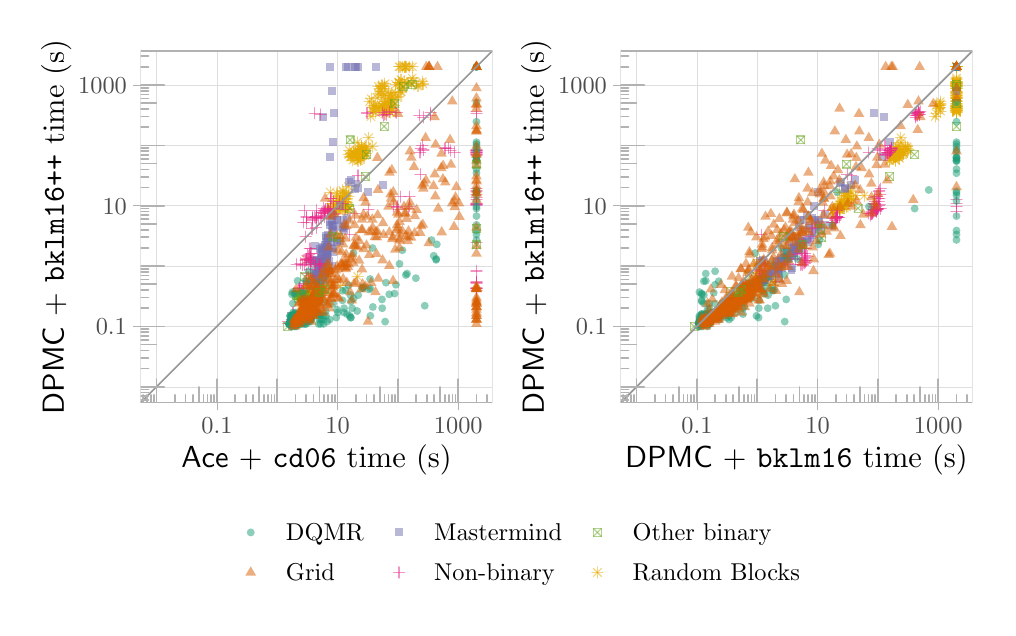
\begin{tikzpicture}[x=1pt,y=1pt]
\definecolor{fillColor}{RGB}{255,255,255}
\path[use as bounding box,fill=fillColor,fill opacity=0.00] (0,0) rectangle (346.90,209.58);
\begin{scope}
\path[clip] (  0.00, 42.80) rectangle (173.45,206.70);
\definecolor{drawColor}{RGB}{255,255,255}
\definecolor{fillColor}{RGB}{255,255,255}

\path[draw=drawColor,line width= 0.6pt,line join=round,line cap=round,fill=fillColor] (  0.00, 42.80) rectangle (173.45,206.70);
\end{scope}
\begin{scope}
\path[clip] ( 40.80, 74.05) rectangle (167.95,201.20);
\definecolor{fillColor}{RGB}{255,255,255}

\path[fill=fillColor] ( 40.80, 74.05) rectangle (167.95,201.20);
\definecolor{drawColor}{gray}{0.87}

\path[draw=drawColor,line width= 0.1pt,line join=round] ( 40.80, 79.83) --
	(167.95, 79.83);

\path[draw=drawColor,line width= 0.1pt,line join=round] ( 40.80,123.44) --
	(167.95,123.44);

\path[draw=drawColor,line width= 0.1pt,line join=round] ( 40.80,167.05) --
	(167.95,167.05);

\path[draw=drawColor,line width= 0.1pt,line join=round] ( 46.58, 74.05) --
	( 46.58,201.20);

\path[draw=drawColor,line width= 0.1pt,line join=round] ( 90.19, 74.05) --
	( 90.19,201.20);

\path[draw=drawColor,line width= 0.1pt,line join=round] (133.80, 74.05) --
	(133.80,201.20);

\path[draw=drawColor,line width= 0.3pt,line join=round] ( 40.80,101.63) --
	(167.95,101.63);

\path[draw=drawColor,line width= 0.3pt,line join=round] ( 40.80,145.24) --
	(167.95,145.24);

\path[draw=drawColor,line width= 0.3pt,line join=round] ( 40.80,188.85) --
	(167.95,188.85);

\path[draw=drawColor,line width= 0.3pt,line join=round] ( 68.39, 74.05) --
	( 68.39,201.20);

\path[draw=drawColor,line width= 0.3pt,line join=round] (111.99, 74.05) --
	(111.99,201.20);

\path[draw=drawColor,line width= 0.3pt,line join=round] (155.60, 74.05) --
	(155.60,201.20);
\definecolor{drawColor}{RGB}{230,171,2}

\path[draw=drawColor,draw opacity=0.50,line width= 0.4pt,line join=round,line cap=round] (101.00,110.29) -- (103.85,113.14);

\path[draw=drawColor,draw opacity=0.50,line width= 0.4pt,line join=round,line cap=round] (101.00,113.14) -- (103.85,110.29);

\path[draw=drawColor,draw opacity=0.50,line width= 0.4pt,line join=round,line cap=round] (100.41,111.72) -- (104.44,111.72);

\path[draw=drawColor,draw opacity=0.50,line width= 0.4pt,line join=round,line cap=round] (102.42,109.70) -- (102.42,113.73);

\path[draw=drawColor,draw opacity=0.50,line width= 0.4pt,line join=round,line cap=round] (102.10,110.29) -- (104.96,113.14);

\path[draw=drawColor,draw opacity=0.50,line width= 0.4pt,line join=round,line cap=round] (102.10,113.14) -- (104.96,110.29);

\path[draw=drawColor,draw opacity=0.50,line width= 0.4pt,line join=round,line cap=round] (101.51,111.72) -- (105.55,111.72);

\path[draw=drawColor,draw opacity=0.50,line width= 0.4pt,line join=round,line cap=round] (103.53,109.70) -- (103.53,113.73);

\path[draw=drawColor,draw opacity=0.50,line width= 0.4pt,line join=round,line cap=round] (100.63,111.80) -- (103.48,114.65);

\path[draw=drawColor,draw opacity=0.50,line width= 0.4pt,line join=round,line cap=round] (100.63,114.65) -- (103.48,111.80);

\path[draw=drawColor,draw opacity=0.50,line width= 0.4pt,line join=round,line cap=round] (100.04,113.22) -- (104.07,113.22);

\path[draw=drawColor,draw opacity=0.50,line width= 0.4pt,line join=round,line cap=round] (102.05,111.20) -- (102.05,115.24);

\path[draw=drawColor,draw opacity=0.50,line width= 0.4pt,line join=round,line cap=round] (102.92,112.34) -- (105.78,115.19);

\path[draw=drawColor,draw opacity=0.50,line width= 0.4pt,line join=round,line cap=round] (102.92,115.19) -- (105.78,112.34);

\path[draw=drawColor,draw opacity=0.50,line width= 0.4pt,line join=round,line cap=round] (102.33,113.76) -- (106.37,113.76);

\path[draw=drawColor,draw opacity=0.50,line width= 0.4pt,line join=round,line cap=round] (104.35,111.75) -- (104.35,115.78);

\path[draw=drawColor,draw opacity=0.50,line width= 0.4pt,line join=round,line cap=round] (102.22,111.51) -- (105.07,114.37);

\path[draw=drawColor,draw opacity=0.50,line width= 0.4pt,line join=round,line cap=round] (102.22,114.37) -- (105.07,111.51);

\path[draw=drawColor,draw opacity=0.50,line width= 0.4pt,line join=round,line cap=round] (101.63,112.94) -- (105.66,112.94);

\path[draw=drawColor,draw opacity=0.50,line width= 0.4pt,line join=round,line cap=round] (103.64,110.92) -- (103.64,114.96);

\path[draw=drawColor,draw opacity=0.50,line width= 0.4pt,line join=round,line cap=round] (101.10,110.29) -- (103.95,113.14);

\path[draw=drawColor,draw opacity=0.50,line width= 0.4pt,line join=round,line cap=round] (101.10,113.14) -- (103.95,110.29);

\path[draw=drawColor,draw opacity=0.50,line width= 0.4pt,line join=round,line cap=round] (100.51,111.72) -- (104.55,111.72);

\path[draw=drawColor,draw opacity=0.50,line width= 0.4pt,line join=round,line cap=round] (102.53,109.70) -- (102.53,113.73);

\path[draw=drawColor,draw opacity=0.50,line width= 0.4pt,line join=round,line cap=round] ( 97.88,110.61) -- (100.74,113.46);

\path[draw=drawColor,draw opacity=0.50,line width= 0.4pt,line join=round,line cap=round] ( 97.88,113.46) -- (100.74,110.61);

\path[draw=drawColor,draw opacity=0.50,line width= 0.4pt,line join=round,line cap=round] ( 97.29,112.04) -- (101.33,112.04);

\path[draw=drawColor,draw opacity=0.50,line width= 0.4pt,line join=round,line cap=round] ( 99.31,110.02) -- ( 99.31,114.05);

\path[draw=drawColor,draw opacity=0.50,line width= 0.4pt,line join=round,line cap=round] (101.50,112.07) -- (104.36,114.92);

\path[draw=drawColor,draw opacity=0.50,line width= 0.4pt,line join=round,line cap=round] (101.50,114.92) -- (104.36,112.07);

\path[draw=drawColor,draw opacity=0.50,line width= 0.4pt,line join=round,line cap=round] (100.91,113.50) -- (104.95,113.50);

\path[draw=drawColor,draw opacity=0.50,line width= 0.4pt,line join=round,line cap=round] (102.93,111.48) -- (102.93,115.51);

\path[draw=drawColor,draw opacity=0.50,line width= 0.4pt,line join=round,line cap=round] (100.65,112.85) -- (103.51,115.70);

\path[draw=drawColor,draw opacity=0.50,line width= 0.4pt,line join=round,line cap=round] (100.65,115.70) -- (103.51,112.85);

\path[draw=drawColor,draw opacity=0.50,line width= 0.4pt,line join=round,line cap=round] (100.06,114.27) -- (104.10,114.27);

\path[draw=drawColor,draw opacity=0.50,line width= 0.4pt,line join=round,line cap=round] (102.08,112.26) -- (102.08,116.29);

\path[draw=drawColor,draw opacity=0.50,line width= 0.4pt,line join=round,line cap=round] ( 99.81,109.96) -- (102.66,112.81);

\path[draw=drawColor,draw opacity=0.50,line width= 0.4pt,line join=round,line cap=round] ( 99.81,112.81) -- (102.66,109.96);

\path[draw=drawColor,draw opacity=0.50,line width= 0.4pt,line join=round,line cap=round] ( 99.22,111.38) -- (103.25,111.38);

\path[draw=drawColor,draw opacity=0.50,line width= 0.4pt,line join=round,line cap=round] (101.23,109.37) -- (101.23,113.40);

\path[draw=drawColor,draw opacity=0.50,line width= 0.4pt,line join=round,line cap=round] ( 98.58,110.92) -- (101.43,113.77);

\path[draw=drawColor,draw opacity=0.50,line width= 0.4pt,line join=round,line cap=round] ( 98.58,113.77) -- (101.43,110.92);

\path[draw=drawColor,draw opacity=0.50,line width= 0.4pt,line join=round,line cap=round] ( 97.99,112.35) -- (102.03,112.35);

\path[draw=drawColor,draw opacity=0.50,line width= 0.4pt,line join=round,line cap=round] (100.01,110.33) -- (100.01,114.36);

\path[draw=drawColor,draw opacity=0.50,line width= 0.4pt,line join=round,line cap=round] (102.31,110.61) -- (105.16,113.46);

\path[draw=drawColor,draw opacity=0.50,line width= 0.4pt,line join=round,line cap=round] (102.31,113.46) -- (105.16,110.61);

\path[draw=drawColor,draw opacity=0.50,line width= 0.4pt,line join=round,line cap=round] (101.72,112.04) -- (105.75,112.04);

\path[draw=drawColor,draw opacity=0.50,line width= 0.4pt,line join=round,line cap=round] (103.73,110.02) -- (103.73,114.05);

\path[draw=drawColor,draw opacity=0.50,line width= 0.4pt,line join=round,line cap=round] (101.00,111.22) -- (103.85,114.07);

\path[draw=drawColor,draw opacity=0.50,line width= 0.4pt,line join=round,line cap=round] (101.00,114.07) -- (103.85,111.22);

\path[draw=drawColor,draw opacity=0.50,line width= 0.4pt,line join=round,line cap=round] (100.41,112.65) -- (104.44,112.65);

\path[draw=drawColor,draw opacity=0.50,line width= 0.4pt,line join=round,line cap=round] (102.42,110.63) -- (102.42,114.67);

\path[draw=drawColor,draw opacity=0.50,line width= 0.4pt,line join=round,line cap=round] (100.32,110.61) -- (103.18,113.46);

\path[draw=drawColor,draw opacity=0.50,line width= 0.4pt,line join=round,line cap=round] (100.32,113.46) -- (103.18,110.61);

\path[draw=drawColor,draw opacity=0.50,line width= 0.4pt,line join=round,line cap=round] ( 99.73,112.04) -- (103.77,112.04);

\path[draw=drawColor,draw opacity=0.50,line width= 0.4pt,line join=round,line cap=round] (101.75,110.02) -- (101.75,114.05);

\path[draw=drawColor,draw opacity=0.50,line width= 0.4pt,line join=round,line cap=round] (102.66,112.07) -- (105.52,114.92);

\path[draw=drawColor,draw opacity=0.50,line width= 0.4pt,line join=round,line cap=round] (102.66,114.92) -- (105.52,112.07);

\path[draw=drawColor,draw opacity=0.50,line width= 0.4pt,line join=round,line cap=round] (102.07,113.50) -- (106.11,113.50);

\path[draw=drawColor,draw opacity=0.50,line width= 0.4pt,line join=round,line cap=round] (104.09,111.48) -- (104.09,115.51);

\path[draw=drawColor,draw opacity=0.50,line width= 0.4pt,line join=round,line cap=round] (102.69,111.22) -- (105.54,114.07);

\path[draw=drawColor,draw opacity=0.50,line width= 0.4pt,line join=round,line cap=round] (102.69,114.07) -- (105.54,111.22);

\path[draw=drawColor,draw opacity=0.50,line width= 0.4pt,line join=round,line cap=round] (102.09,112.65) -- (106.13,112.65);

\path[draw=drawColor,draw opacity=0.50,line width= 0.4pt,line join=round,line cap=round] (104.11,110.63) -- (104.11,114.67);

\path[draw=drawColor,draw opacity=0.50,line width= 0.4pt,line join=round,line cap=round] (102.58,114.86) -- (105.43,117.71);

\path[draw=drawColor,draw opacity=0.50,line width= 0.4pt,line join=round,line cap=round] (102.58,117.71) -- (105.43,114.86);

\path[draw=drawColor,draw opacity=0.50,line width= 0.4pt,line join=round,line cap=round] (101.99,116.29) -- (106.02,116.29);

\path[draw=drawColor,draw opacity=0.50,line width= 0.4pt,line join=round,line cap=round] (104.00,114.27) -- (104.00,118.31);

\path[draw=drawColor,draw opacity=0.50,line width= 0.4pt,line join=round,line cap=round] (103.11,113.57) -- (105.96,116.42);

\path[draw=drawColor,draw opacity=0.50,line width= 0.4pt,line join=round,line cap=round] (103.11,116.42) -- (105.96,113.57);

\path[draw=drawColor,draw opacity=0.50,line width= 0.4pt,line join=round,line cap=round] (102.52,114.99) -- (106.56,114.99);

\path[draw=drawColor,draw opacity=0.50,line width= 0.4pt,line join=round,line cap=round] (104.54,112.98) -- (104.54,117.01);

\path[draw=drawColor,draw opacity=0.50,line width= 0.4pt,line join=round,line cap=round] (100.52,112.60) -- (103.37,115.45);

\path[draw=drawColor,draw opacity=0.50,line width= 0.4pt,line join=round,line cap=round] (100.52,115.45) -- (103.37,112.60);

\path[draw=drawColor,draw opacity=0.50,line width= 0.4pt,line join=round,line cap=round] ( 99.93,114.02) -- (103.96,114.02);

\path[draw=drawColor,draw opacity=0.50,line width= 0.4pt,line join=round,line cap=round] (101.94,112.00) -- (101.94,116.04);

\path[draw=drawColor,draw opacity=0.50,line width= 0.4pt,line join=round,line cap=round] (103.64,113.09) -- (106.49,115.95);

\path[draw=drawColor,draw opacity=0.50,line width= 0.4pt,line join=round,line cap=round] (103.64,115.95) -- (106.49,113.09);

\path[draw=drawColor,draw opacity=0.50,line width= 0.4pt,line join=round,line cap=round] (103.05,114.52) -- (107.08,114.52);

\path[draw=drawColor,draw opacity=0.50,line width= 0.4pt,line join=round,line cap=round] (105.06,112.50) -- (105.06,116.54);

\path[draw=drawColor,draw opacity=0.50,line width= 0.4pt,line join=round,line cap=round] (101.00,114.45) -- (103.85,117.30);

\path[draw=drawColor,draw opacity=0.50,line width= 0.4pt,line join=round,line cap=round] (101.00,117.30) -- (103.85,114.45);

\path[draw=drawColor,draw opacity=0.50,line width= 0.4pt,line join=round,line cap=round] (100.41,115.88) -- (104.44,115.88);

\path[draw=drawColor,draw opacity=0.50,line width= 0.4pt,line join=round,line cap=round] (102.42,113.86) -- (102.42,117.89);

\path[draw=drawColor,draw opacity=0.50,line width= 0.4pt,line join=round,line cap=round] (101.00,112.07) -- (103.85,114.92);

\path[draw=drawColor,draw opacity=0.50,line width= 0.4pt,line join=round,line cap=round] (101.00,114.92) -- (103.85,112.07);

\path[draw=drawColor,draw opacity=0.50,line width= 0.4pt,line join=round,line cap=round] (100.41,113.50) -- (104.44,113.50);

\path[draw=drawColor,draw opacity=0.50,line width= 0.4pt,line join=round,line cap=round] (102.42,111.48) -- (102.42,115.51);

\path[draw=drawColor,draw opacity=0.50,line width= 0.4pt,line join=round,line cap=round] ( 99.20,124.27) -- (102.05,127.13);

\path[draw=drawColor,draw opacity=0.50,line width= 0.4pt,line join=round,line cap=round] ( 99.20,127.13) -- (102.05,124.27);

\path[draw=drawColor,draw opacity=0.50,line width= 0.4pt,line join=round,line cap=round] ( 98.61,125.70) -- (102.64,125.70);

\path[draw=drawColor,draw opacity=0.50,line width= 0.4pt,line join=round,line cap=round] (100.63,123.68) -- (100.63,127.72);

\path[draw=drawColor,draw opacity=0.50,line width= 0.4pt,line join=round,line cap=round] (100.57,112.07) -- (103.43,114.92);

\path[draw=drawColor,draw opacity=0.50,line width= 0.4pt,line join=round,line cap=round] (100.57,114.92) -- (103.43,112.07);

\path[draw=drawColor,draw opacity=0.50,line width= 0.4pt,line join=round,line cap=round] ( 99.98,113.50) -- (104.02,113.50);

\path[draw=drawColor,draw opacity=0.50,line width= 0.4pt,line join=round,line cap=round] (102.00,111.48) -- (102.00,115.51);

\path[draw=drawColor,draw opacity=0.50,line width= 0.4pt,line join=round,line cap=round] (100.18,112.07) -- (103.04,114.92);

\path[draw=drawColor,draw opacity=0.50,line width= 0.4pt,line join=round,line cap=round] (100.18,114.92) -- (103.04,112.07);

\path[draw=drawColor,draw opacity=0.50,line width= 0.4pt,line join=round,line cap=round] ( 99.59,113.50) -- (103.63,113.50);

\path[draw=drawColor,draw opacity=0.50,line width= 0.4pt,line join=round,line cap=round] (101.61,111.48) -- (101.61,115.51);

\path[draw=drawColor,draw opacity=0.50,line width= 0.4pt,line join=round,line cap=round] (102.58,113.57) -- (105.43,116.42);

\path[draw=drawColor,draw opacity=0.50,line width= 0.4pt,line join=round,line cap=round] (102.58,116.42) -- (105.43,113.57);

\path[draw=drawColor,draw opacity=0.50,line width= 0.4pt,line join=round,line cap=round] (101.99,114.99) -- (106.02,114.99);

\path[draw=drawColor,draw opacity=0.50,line width= 0.4pt,line join=round,line cap=round] (104.00,112.98) -- (104.00,117.01);

\path[draw=drawColor,draw opacity=0.50,line width= 0.4pt,line join=round,line cap=round] (103.24,115.63) -- (106.09,118.49);

\path[draw=drawColor,draw opacity=0.50,line width= 0.4pt,line join=round,line cap=round] (103.24,118.49) -- (106.09,115.63);

\path[draw=drawColor,draw opacity=0.50,line width= 0.4pt,line join=round,line cap=round] (102.64,117.06) -- (106.68,117.06);

\path[draw=drawColor,draw opacity=0.50,line width= 0.4pt,line join=round,line cap=round] (104.66,115.04) -- (104.66,119.08);

\path[draw=drawColor,draw opacity=0.50,line width= 0.4pt,line join=round,line cap=round] (102.15,112.85) -- (105.00,115.70);

\path[draw=drawColor,draw opacity=0.50,line width= 0.4pt,line join=round,line cap=round] (102.15,115.70) -- (105.00,112.85);

\path[draw=drawColor,draw opacity=0.50,line width= 0.4pt,line join=round,line cap=round] (101.56,114.27) -- (105.59,114.27);

\path[draw=drawColor,draw opacity=0.50,line width= 0.4pt,line join=round,line cap=round] (103.57,112.26) -- (103.57,116.29);

\path[draw=drawColor,draw opacity=0.50,line width= 0.4pt,line join=round,line cap=round] ( 99.95,111.51) -- (102.81,114.37);

\path[draw=drawColor,draw opacity=0.50,line width= 0.4pt,line join=round,line cap=round] ( 99.95,114.37) -- (102.81,111.51);

\path[draw=drawColor,draw opacity=0.50,line width= 0.4pt,line join=round,line cap=round] ( 99.36,112.94) -- (103.40,112.94);

\path[draw=drawColor,draw opacity=0.50,line width= 0.4pt,line join=round,line cap=round] (101.38,110.92) -- (101.38,114.96);

\path[draw=drawColor,draw opacity=0.50,line width= 0.4pt,line join=round,line cap=round] (101.02,113.33) -- (103.88,116.19);

\path[draw=drawColor,draw opacity=0.50,line width= 0.4pt,line join=round,line cap=round] (101.02,116.19) -- (103.88,113.33);

\path[draw=drawColor,draw opacity=0.50,line width= 0.4pt,line join=round,line cap=round] (100.43,114.76) -- (104.47,114.76);

\path[draw=drawColor,draw opacity=0.50,line width= 0.4pt,line join=round,line cap=round] (102.45,112.74) -- (102.45,116.78);

\path[draw=drawColor,draw opacity=0.50,line width= 0.4pt,line join=round,line cap=round] ( 99.87,111.51) -- (102.72,114.37);

\path[draw=drawColor,draw opacity=0.50,line width= 0.4pt,line join=round,line cap=round] ( 99.87,114.37) -- (102.72,111.51);

\path[draw=drawColor,draw opacity=0.50,line width= 0.4pt,line join=round,line cap=round] ( 99.28,112.94) -- (103.31,112.94);

\path[draw=drawColor,draw opacity=0.50,line width= 0.4pt,line join=round,line cap=round] (101.29,110.92) -- (101.29,114.96);

\path[draw=drawColor,draw opacity=0.50,line width= 0.4pt,line join=round,line cap=round] (101.28,115.06) -- (104.13,117.91);

\path[draw=drawColor,draw opacity=0.50,line width= 0.4pt,line join=round,line cap=round] (101.28,117.91) -- (104.13,115.06);

\path[draw=drawColor,draw opacity=0.50,line width= 0.4pt,line join=round,line cap=round] (100.69,116.49) -- (104.72,116.49);

\path[draw=drawColor,draw opacity=0.50,line width= 0.4pt,line join=round,line cap=round] (102.71,114.47) -- (102.71,118.50);

\path[draw=drawColor,draw opacity=0.50,line width= 0.4pt,line join=round,line cap=round] (103.93,122.38) -- (106.78,125.24);

\path[draw=drawColor,draw opacity=0.50,line width= 0.4pt,line join=round,line cap=round] (103.93,125.24) -- (106.78,122.38);

\path[draw=drawColor,draw opacity=0.50,line width= 0.4pt,line join=round,line cap=round] (103.34,123.81) -- (107.37,123.81);

\path[draw=drawColor,draw opacity=0.50,line width= 0.4pt,line join=round,line cap=round] (105.35,121.79) -- (105.35,125.83);

\path[draw=drawColor,draw opacity=0.50,line width= 0.4pt,line join=round,line cap=round] (100.81,114.86) -- (103.67,117.71);

\path[draw=drawColor,draw opacity=0.50,line width= 0.4pt,line join=round,line cap=round] (100.81,117.71) -- (103.67,114.86);

\path[draw=drawColor,draw opacity=0.50,line width= 0.4pt,line join=round,line cap=round] (100.22,116.29) -- (104.26,116.29);

\path[draw=drawColor,draw opacity=0.50,line width= 0.4pt,line join=round,line cap=round] (102.24,114.27) -- (102.24,118.31);

\path[draw=drawColor,draw opacity=0.50,line width= 0.4pt,line join=round,line cap=round] (100.55,114.02) -- (103.40,116.87);

\path[draw=drawColor,draw opacity=0.50,line width= 0.4pt,line join=round,line cap=round] (100.55,116.87) -- (103.40,114.02);

\path[draw=drawColor,draw opacity=0.50,line width= 0.4pt,line join=round,line cap=round] ( 99.95,115.45) -- (103.99,115.45);

\path[draw=drawColor,draw opacity=0.50,line width= 0.4pt,line join=round,line cap=round] (101.97,113.43) -- (101.97,117.46);

\path[draw=drawColor,draw opacity=0.50,line width= 0.4pt,line join=round,line cap=round] (101.99,114.66) -- (104.84,117.51);

\path[draw=drawColor,draw opacity=0.50,line width= 0.4pt,line join=round,line cap=round] (101.99,117.51) -- (104.84,114.66);

\path[draw=drawColor,draw opacity=0.50,line width= 0.4pt,line join=round,line cap=round] (101.39,116.08) -- (105.43,116.08);

\path[draw=drawColor,draw opacity=0.50,line width= 0.4pt,line join=round,line cap=round] (103.41,114.07) -- (103.41,118.10);

\path[draw=drawColor,draw opacity=0.50,line width= 0.4pt,line join=round,line cap=round] (103.81,116.00) -- (106.67,118.85);

\path[draw=drawColor,draw opacity=0.50,line width= 0.4pt,line join=round,line cap=round] (103.81,118.85) -- (106.67,116.00);

\path[draw=drawColor,draw opacity=0.50,line width= 0.4pt,line join=round,line cap=round] (103.22,117.43) -- (107.26,117.43);

\path[draw=drawColor,draw opacity=0.50,line width= 0.4pt,line join=round,line cap=round] (105.24,115.41) -- (105.24,119.44);

\path[draw=drawColor,draw opacity=0.50,line width= 0.4pt,line join=round,line cap=round] (101.10,113.33) -- (103.95,116.19);

\path[draw=drawColor,draw opacity=0.50,line width= 0.4pt,line join=round,line cap=round] (101.10,116.19) -- (103.95,113.33);

\path[draw=drawColor,draw opacity=0.50,line width= 0.4pt,line join=round,line cap=round] (100.51,114.76) -- (104.55,114.76);

\path[draw=drawColor,draw opacity=0.50,line width= 0.4pt,line join=round,line cap=round] (102.53,112.74) -- (102.53,116.78);

\path[draw=drawColor,draw opacity=0.50,line width= 0.4pt,line join=round,line cap=round] (102.75,119.66) -- (105.60,122.51);

\path[draw=drawColor,draw opacity=0.50,line width= 0.4pt,line join=round,line cap=round] (102.75,122.51) -- (105.60,119.66);

\path[draw=drawColor,draw opacity=0.50,line width= 0.4pt,line join=round,line cap=round] (102.16,121.08) -- (106.19,121.08);

\path[draw=drawColor,draw opacity=0.50,line width= 0.4pt,line join=round,line cap=round] (104.18,119.07) -- (104.18,123.10);

\path[draw=drawColor,draw opacity=0.50,line width= 0.4pt,line join=round,line cap=round] (102.51,116.69) -- (105.36,119.54);

\path[draw=drawColor,draw opacity=0.50,line width= 0.4pt,line join=round,line cap=round] (102.51,119.54) -- (105.36,116.69);

\path[draw=drawColor,draw opacity=0.50,line width= 0.4pt,line join=round,line cap=round] (101.92,118.11) -- (105.95,118.11);

\path[draw=drawColor,draw opacity=0.50,line width= 0.4pt,line join=round,line cap=round] (103.94,116.10) -- (103.94,120.13);

\path[draw=drawColor,draw opacity=0.50,line width= 0.4pt,line join=round,line cap=round] (103.52,115.26) -- (106.37,118.11);

\path[draw=drawColor,draw opacity=0.50,line width= 0.4pt,line join=round,line cap=round] (103.52,118.11) -- (106.37,115.26);

\path[draw=drawColor,draw opacity=0.50,line width= 0.4pt,line join=round,line cap=round] (102.93,116.68) -- (106.96,116.68);

\path[draw=drawColor,draw opacity=0.50,line width= 0.4pt,line join=round,line cap=round] (104.95,114.66) -- (104.95,118.70);

\path[draw=drawColor,draw opacity=0.50,line width= 0.4pt,line join=round,line cap=round] (103.21,123.08) -- (106.07,125.94);

\path[draw=drawColor,draw opacity=0.50,line width= 0.4pt,line join=round,line cap=round] (103.21,125.94) -- (106.07,123.08);

\path[draw=drawColor,draw opacity=0.50,line width= 0.4pt,line join=round,line cap=round] (102.62,124.51) -- (106.66,124.51);

\path[draw=drawColor,draw opacity=0.50,line width= 0.4pt,line join=round,line cap=round] (104.64,122.49) -- (104.64,126.53);

\path[draw=drawColor,draw opacity=0.50,line width= 0.4pt,line join=round,line cap=round] (111.56,114.86) -- (114.41,117.71);

\path[draw=drawColor,draw opacity=0.50,line width= 0.4pt,line join=round,line cap=round] (111.56,117.71) -- (114.41,114.86);

\path[draw=drawColor,draw opacity=0.50,line width= 0.4pt,line join=round,line cap=round] (110.97,116.29) -- (115.00,116.29);

\path[draw=drawColor,draw opacity=0.50,line width= 0.4pt,line join=round,line cap=round] (112.98,114.27) -- (112.98,118.31);

\path[draw=drawColor,draw opacity=0.50,line width= 0.4pt,line join=round,line cap=round] (101.20,114.02) -- (104.06,116.87);

\path[draw=drawColor,draw opacity=0.50,line width= 0.4pt,line join=round,line cap=round] (101.20,116.87) -- (104.06,114.02);

\path[draw=drawColor,draw opacity=0.50,line width= 0.4pt,line join=round,line cap=round] (100.61,115.45) -- (104.65,115.45);

\path[draw=drawColor,draw opacity=0.50,line width= 0.4pt,line join=round,line cap=round] (102.63,113.43) -- (102.63,117.46);

\path[draw=drawColor,draw opacity=0.50,line width= 0.4pt,line join=round,line cap=round] (100.16,113.57) -- (103.01,116.42);

\path[draw=drawColor,draw opacity=0.50,line width= 0.4pt,line join=round,line cap=round] (100.16,116.42) -- (103.01,113.57);

\path[draw=drawColor,draw opacity=0.50,line width= 0.4pt,line join=round,line cap=round] ( 99.56,114.99) -- (103.60,114.99);

\path[draw=drawColor,draw opacity=0.50,line width= 0.4pt,line join=round,line cap=round] (101.58,112.98) -- (101.58,117.01);

\path[draw=drawColor,draw opacity=0.50,line width= 0.4pt,line join=round,line cap=round] (105.60,114.66) -- (108.46,117.51);

\path[draw=drawColor,draw opacity=0.50,line width= 0.4pt,line join=round,line cap=round] (105.60,117.51) -- (108.46,114.66);

\path[draw=drawColor,draw opacity=0.50,line width= 0.4pt,line join=round,line cap=round] (105.01,116.08) -- (109.05,116.08);

\path[draw=drawColor,draw opacity=0.50,line width= 0.4pt,line join=round,line cap=round] (107.03,114.07) -- (107.03,118.10);

\path[draw=drawColor,draw opacity=0.50,line width= 0.4pt,line join=round,line cap=round] (101.20,114.66) -- (104.06,117.51);

\path[draw=drawColor,draw opacity=0.50,line width= 0.4pt,line join=round,line cap=round] (101.20,117.51) -- (104.06,114.66);

\path[draw=drawColor,draw opacity=0.50,line width= 0.4pt,line join=round,line cap=round] (100.61,116.08) -- (104.65,116.08);

\path[draw=drawColor,draw opacity=0.50,line width= 0.4pt,line join=round,line cap=round] (102.63,114.07) -- (102.63,118.10);

\path[draw=drawColor,draw opacity=0.50,line width= 0.4pt,line join=round,line cap=round] (104.38,117.33) -- (107.23,120.18);

\path[draw=drawColor,draw opacity=0.50,line width= 0.4pt,line join=round,line cap=round] (104.38,120.18) -- (107.23,117.33);

\path[draw=drawColor,draw opacity=0.50,line width= 0.4pt,line join=round,line cap=round] (103.78,118.76) -- (107.82,118.76);

\path[draw=drawColor,draw opacity=0.50,line width= 0.4pt,line join=round,line cap=round] (105.80,116.74) -- (105.80,120.77);

\path[draw=drawColor,draw opacity=0.50,line width= 0.4pt,line join=round,line cap=round] (112.41,142.42) -- (115.27,145.27);

\path[draw=drawColor,draw opacity=0.50,line width= 0.4pt,line join=round,line cap=round] (112.41,145.27) -- (115.27,142.42);

\path[draw=drawColor,draw opacity=0.50,line width= 0.4pt,line join=round,line cap=round] (111.82,143.85) -- (115.86,143.85);

\path[draw=drawColor,draw opacity=0.50,line width= 0.4pt,line join=round,line cap=round] (113.84,141.83) -- (113.84,145.86);

\path[draw=drawColor,draw opacity=0.50,line width= 0.4pt,line join=round,line cap=round] (111.35,143.77) -- (114.20,146.62);

\path[draw=drawColor,draw opacity=0.50,line width= 0.4pt,line join=round,line cap=round] (111.35,146.62) -- (114.20,143.77);

\path[draw=drawColor,draw opacity=0.50,line width= 0.4pt,line join=round,line cap=round] (110.76,145.20) -- (114.79,145.20);

\path[draw=drawColor,draw opacity=0.50,line width= 0.4pt,line join=round,line cap=round] (112.78,143.18) -- (112.78,147.21);

\path[draw=drawColor,draw opacity=0.50,line width= 0.4pt,line join=round,line cap=round] (107.58,142.45) -- (110.43,145.31);

\path[draw=drawColor,draw opacity=0.50,line width= 0.4pt,line join=round,line cap=round] (107.58,145.31) -- (110.43,142.45);

\path[draw=drawColor,draw opacity=0.50,line width= 0.4pt,line join=round,line cap=round] (106.98,143.88) -- (111.02,143.88);

\path[draw=drawColor,draw opacity=0.50,line width= 0.4pt,line join=round,line cap=round] (109.00,141.86) -- (109.00,145.90);

\path[draw=drawColor,draw opacity=0.50,line width= 0.4pt,line join=round,line cap=round] (111.02,142.02) -- (113.87,144.87);

\path[draw=drawColor,draw opacity=0.50,line width= 0.4pt,line join=round,line cap=round] (111.02,144.87) -- (113.87,142.02);

\path[draw=drawColor,draw opacity=0.50,line width= 0.4pt,line join=round,line cap=round] (110.43,143.44) -- (114.47,143.44);

\path[draw=drawColor,draw opacity=0.50,line width= 0.4pt,line join=round,line cap=round] (112.45,141.43) -- (112.45,145.46);

\path[draw=drawColor,draw opacity=0.50,line width= 0.4pt,line join=round,line cap=round] (114.13,142.51) -- (116.98,145.36);

\path[draw=drawColor,draw opacity=0.50,line width= 0.4pt,line join=round,line cap=round] (114.13,145.36) -- (116.98,142.51);

\path[draw=drawColor,draw opacity=0.50,line width= 0.4pt,line join=round,line cap=round] (113.54,143.93) -- (117.57,143.93);

\path[draw=drawColor,draw opacity=0.50,line width= 0.4pt,line join=round,line cap=round] (115.55,141.92) -- (115.55,145.95);

\path[draw=drawColor,draw opacity=0.50,line width= 0.4pt,line join=round,line cap=round] (114.29,142.48) -- (117.15,145.33);

\path[draw=drawColor,draw opacity=0.50,line width= 0.4pt,line join=round,line cap=round] (114.29,145.33) -- (117.15,142.48);

\path[draw=drawColor,draw opacity=0.50,line width= 0.4pt,line join=round,line cap=round] (113.70,143.90) -- (117.74,143.90);

\path[draw=drawColor,draw opacity=0.50,line width= 0.4pt,line join=round,line cap=round] (115.72,141.88) -- (115.72,145.92);

\path[draw=drawColor,draw opacity=0.50,line width= 0.4pt,line join=round,line cap=round] (108.14,143.25) -- (111.00,146.10);

\path[draw=drawColor,draw opacity=0.50,line width= 0.4pt,line join=round,line cap=round] (108.14,146.10) -- (111.00,143.25);

\path[draw=drawColor,draw opacity=0.50,line width= 0.4pt,line join=round,line cap=round] (107.55,144.68) -- (111.59,144.68);

\path[draw=drawColor,draw opacity=0.50,line width= 0.4pt,line join=round,line cap=round] (109.57,142.66) -- (109.57,146.69);

\path[draw=drawColor,draw opacity=0.50,line width= 0.4pt,line join=round,line cap=round] (108.96,142.50) -- (111.82,145.35);

\path[draw=drawColor,draw opacity=0.50,line width= 0.4pt,line join=round,line cap=round] (108.96,145.35) -- (111.82,142.50);

\path[draw=drawColor,draw opacity=0.50,line width= 0.4pt,line join=round,line cap=round] (108.37,143.92) -- (112.41,143.92);

\path[draw=drawColor,draw opacity=0.50,line width= 0.4pt,line join=round,line cap=round] (110.39,141.91) -- (110.39,145.94);

\path[draw=drawColor,draw opacity=0.50,line width= 0.4pt,line join=round,line cap=round] (108.95,142.50) -- (111.80,145.35);

\path[draw=drawColor,draw opacity=0.50,line width= 0.4pt,line join=round,line cap=round] (108.95,145.35) -- (111.80,142.50);

\path[draw=drawColor,draw opacity=0.50,line width= 0.4pt,line join=round,line cap=round] (108.36,143.92) -- (112.40,143.92);

\path[draw=drawColor,draw opacity=0.50,line width= 0.4pt,line join=round,line cap=round] (110.38,141.91) -- (110.38,145.94);

\path[draw=drawColor,draw opacity=0.50,line width= 0.4pt,line join=round,line cap=round] (108.51,142.82) -- (111.37,145.67);

\path[draw=drawColor,draw opacity=0.50,line width= 0.4pt,line join=round,line cap=round] (108.51,145.67) -- (111.37,142.82);

\path[draw=drawColor,draw opacity=0.50,line width= 0.4pt,line join=round,line cap=round] (107.92,144.24) -- (111.96,144.24);

\path[draw=drawColor,draw opacity=0.50,line width= 0.4pt,line join=round,line cap=round] (109.94,142.23) -- (109.94,146.26);

\path[draw=drawColor,draw opacity=0.50,line width= 0.4pt,line join=round,line cap=round] (107.03,141.94) -- (109.88,144.79);

\path[draw=drawColor,draw opacity=0.50,line width= 0.4pt,line join=round,line cap=round] (107.03,144.79) -- (109.88,141.94);

\path[draw=drawColor,draw opacity=0.50,line width= 0.4pt,line join=round,line cap=round] (106.44,143.36) -- (110.47,143.36);

\path[draw=drawColor,draw opacity=0.50,line width= 0.4pt,line join=round,line cap=round] (108.45,141.35) -- (108.45,145.38);

\path[draw=drawColor,draw opacity=0.50,line width= 0.4pt,line join=round,line cap=round] (112.97,142.35) -- (115.83,145.21);

\path[draw=drawColor,draw opacity=0.50,line width= 0.4pt,line join=round,line cap=round] (112.97,145.21) -- (115.83,142.35);

\path[draw=drawColor,draw opacity=0.50,line width= 0.4pt,line join=round,line cap=round] (112.38,143.78) -- (116.42,143.78);

\path[draw=drawColor,draw opacity=0.50,line width= 0.4pt,line join=round,line cap=round] (114.40,141.76) -- (114.40,145.80);

\path[draw=drawColor,draw opacity=0.50,line width= 0.4pt,line join=round,line cap=round] (114.53,143.63) -- (117.39,146.49);

\path[draw=drawColor,draw opacity=0.50,line width= 0.4pt,line join=round,line cap=round] (114.53,146.49) -- (117.39,143.63);

\path[draw=drawColor,draw opacity=0.50,line width= 0.4pt,line join=round,line cap=round] (113.94,145.06) -- (117.98,145.06);

\path[draw=drawColor,draw opacity=0.50,line width= 0.4pt,line join=round,line cap=round] (115.96,143.04) -- (115.96,147.08);

\path[draw=drawColor,draw opacity=0.50,line width= 0.4pt,line join=round,line cap=round] (112.89,143.20) -- (115.74,146.05);

\path[draw=drawColor,draw opacity=0.50,line width= 0.4pt,line join=round,line cap=round] (112.89,146.05) -- (115.74,143.20);

\path[draw=drawColor,draw opacity=0.50,line width= 0.4pt,line join=round,line cap=round] (112.30,144.63) -- (116.34,144.63);

\path[draw=drawColor,draw opacity=0.50,line width= 0.4pt,line join=round,line cap=round] (114.32,142.61) -- (114.32,146.64);

\path[draw=drawColor,draw opacity=0.50,line width= 0.4pt,line join=round,line cap=round] (110.41,142.27) -- (113.26,145.12);

\path[draw=drawColor,draw opacity=0.50,line width= 0.4pt,line join=round,line cap=round] (110.41,145.12) -- (113.26,142.27);

\path[draw=drawColor,draw opacity=0.50,line width= 0.4pt,line join=round,line cap=round] (109.81,143.69) -- (113.85,143.69);

\path[draw=drawColor,draw opacity=0.50,line width= 0.4pt,line join=round,line cap=round] (111.83,141.67) -- (111.83,145.71);

\path[draw=drawColor,draw opacity=0.50,line width= 0.4pt,line join=round,line cap=round] (111.53,145.39) -- (114.38,148.24);

\path[draw=drawColor,draw opacity=0.50,line width= 0.4pt,line join=round,line cap=round] (111.53,148.24) -- (114.38,145.39);

\path[draw=drawColor,draw opacity=0.50,line width= 0.4pt,line join=round,line cap=round] (110.94,146.82) -- (114.98,146.82);

\path[draw=drawColor,draw opacity=0.50,line width= 0.4pt,line join=round,line cap=round] (112.96,144.80) -- (112.96,148.84);

\path[draw=drawColor,draw opacity=0.50,line width= 0.4pt,line join=round,line cap=round] (112.81,145.41) -- (115.66,148.26);

\path[draw=drawColor,draw opacity=0.50,line width= 0.4pt,line join=round,line cap=round] (112.81,148.26) -- (115.66,145.41);

\path[draw=drawColor,draw opacity=0.50,line width= 0.4pt,line join=round,line cap=round] (112.22,146.83) -- (116.25,146.83);

\path[draw=drawColor,draw opacity=0.50,line width= 0.4pt,line join=round,line cap=round] (114.24,144.82) -- (114.24,148.85);

\path[draw=drawColor,draw opacity=0.50,line width= 0.4pt,line join=round,line cap=round] (107.86,148.75) -- (110.71,151.60);

\path[draw=drawColor,draw opacity=0.50,line width= 0.4pt,line join=round,line cap=round] (107.86,151.60) -- (110.71,148.75);

\path[draw=drawColor,draw opacity=0.50,line width= 0.4pt,line join=round,line cap=round] (107.27,150.17) -- (111.30,150.17);

\path[draw=drawColor,draw opacity=0.50,line width= 0.4pt,line join=round,line cap=round] (109.28,148.15) -- (109.28,152.19);

\path[draw=drawColor,draw opacity=0.50,line width= 0.4pt,line join=round,line cap=round] (110.21,145.83) -- (113.06,148.68);

\path[draw=drawColor,draw opacity=0.50,line width= 0.4pt,line join=round,line cap=round] (110.21,148.68) -- (113.06,145.83);

\path[draw=drawColor,draw opacity=0.50,line width= 0.4pt,line join=round,line cap=round] (109.62,147.26) -- (113.66,147.26);

\path[draw=drawColor,draw opacity=0.50,line width= 0.4pt,line join=round,line cap=round] (111.64,145.24) -- (111.64,149.27);

\path[draw=drawColor,draw opacity=0.50,line width= 0.4pt,line join=round,line cap=round] (111.40,143.16) -- (114.25,146.01);

\path[draw=drawColor,draw opacity=0.50,line width= 0.4pt,line join=round,line cap=round] (111.40,146.01) -- (114.25,143.16);

\path[draw=drawColor,draw opacity=0.50,line width= 0.4pt,line join=round,line cap=round] (110.81,144.59) -- (114.85,144.59);

\path[draw=drawColor,draw opacity=0.50,line width= 0.4pt,line join=round,line cap=round] (112.83,142.57) -- (112.83,146.60);

\path[draw=drawColor,draw opacity=0.50,line width= 0.4pt,line join=round,line cap=round] (114.21,143.60) -- (117.06,146.45);

\path[draw=drawColor,draw opacity=0.50,line width= 0.4pt,line join=round,line cap=round] (114.21,146.45) -- (117.06,143.60);

\path[draw=drawColor,draw opacity=0.50,line width= 0.4pt,line join=round,line cap=round] (113.62,145.02) -- (117.65,145.02);

\path[draw=drawColor,draw opacity=0.50,line width= 0.4pt,line join=round,line cap=round] (115.64,143.00) -- (115.64,147.04);

\path[draw=drawColor,draw opacity=0.50,line width= 0.4pt,line join=round,line cap=round] (110.26,143.39) -- (113.11,146.24);

\path[draw=drawColor,draw opacity=0.50,line width= 0.4pt,line join=round,line cap=round] (110.26,146.24) -- (113.11,143.39);

\path[draw=drawColor,draw opacity=0.50,line width= 0.4pt,line join=round,line cap=round] (109.67,144.82) -- (113.70,144.82);

\path[draw=drawColor,draw opacity=0.50,line width= 0.4pt,line join=round,line cap=round] (111.69,142.80) -- (111.69,146.83);

\path[draw=drawColor,draw opacity=0.50,line width= 0.4pt,line join=round,line cap=round] (110.18,143.13) -- (113.03,145.98);

\path[draw=drawColor,draw opacity=0.50,line width= 0.4pt,line join=round,line cap=round] (110.18,145.98) -- (113.03,143.13);

\path[draw=drawColor,draw opacity=0.50,line width= 0.4pt,line join=round,line cap=round] (109.59,144.56) -- (113.63,144.56);

\path[draw=drawColor,draw opacity=0.50,line width= 0.4pt,line join=round,line cap=round] (111.61,142.54) -- (111.61,146.57);

\path[draw=drawColor,draw opacity=0.50,line width= 0.4pt,line join=round,line cap=round] (110.25,144.70) -- (113.10,147.55);

\path[draw=drawColor,draw opacity=0.50,line width= 0.4pt,line join=round,line cap=round] (110.25,147.55) -- (113.10,144.70);

\path[draw=drawColor,draw opacity=0.50,line width= 0.4pt,line join=round,line cap=round] (109.66,146.13) -- (113.69,146.13);

\path[draw=drawColor,draw opacity=0.50,line width= 0.4pt,line join=round,line cap=round] (111.68,144.11) -- (111.68,148.15);

\path[draw=drawColor,draw opacity=0.50,line width= 0.4pt,line join=round,line cap=round] (110.77,143.12) -- (113.62,145.97);

\path[draw=drawColor,draw opacity=0.50,line width= 0.4pt,line join=round,line cap=round] (110.77,145.97) -- (113.62,143.12);

\path[draw=drawColor,draw opacity=0.50,line width= 0.4pt,line join=round,line cap=round] (110.17,144.55) -- (114.21,144.55);

\path[draw=drawColor,draw opacity=0.50,line width= 0.4pt,line join=round,line cap=round] (112.19,142.53) -- (112.19,146.56);

\path[draw=drawColor,draw opacity=0.50,line width= 0.4pt,line join=round,line cap=round] (108.07,143.07) -- (110.92,145.92);

\path[draw=drawColor,draw opacity=0.50,line width= 0.4pt,line join=round,line cap=round] (108.07,145.92) -- (110.92,143.07);

\path[draw=drawColor,draw opacity=0.50,line width= 0.4pt,line join=round,line cap=round] (107.48,144.49) -- (111.51,144.49);

\path[draw=drawColor,draw opacity=0.50,line width= 0.4pt,line join=round,line cap=round] (109.50,142.48) -- (109.50,146.51);

\path[draw=drawColor,draw opacity=0.50,line width= 0.4pt,line join=round,line cap=round] (109.00,144.77) -- (111.85,147.62);

\path[draw=drawColor,draw opacity=0.50,line width= 0.4pt,line join=round,line cap=round] (109.00,147.62) -- (111.85,144.77);

\path[draw=drawColor,draw opacity=0.50,line width= 0.4pt,line join=round,line cap=round] (108.40,146.20) -- (112.44,146.20);

\path[draw=drawColor,draw opacity=0.50,line width= 0.4pt,line join=round,line cap=round] (110.42,144.18) -- (110.42,148.21);

\path[draw=drawColor,draw opacity=0.50,line width= 0.4pt,line join=round,line cap=round] (114.59,142.96) -- (117.44,145.82);

\path[draw=drawColor,draw opacity=0.50,line width= 0.4pt,line join=round,line cap=round] (114.59,145.82) -- (117.44,142.96);

\path[draw=drawColor,draw opacity=0.50,line width= 0.4pt,line join=round,line cap=round] (114.00,144.39) -- (118.03,144.39);

\path[draw=drawColor,draw opacity=0.50,line width= 0.4pt,line join=round,line cap=round] (116.02,142.37) -- (116.02,146.41);

\path[draw=drawColor,draw opacity=0.50,line width= 0.4pt,line join=round,line cap=round] (111.25,145.79) -- (114.11,148.64);

\path[draw=drawColor,draw opacity=0.50,line width= 0.4pt,line join=round,line cap=round] (111.25,148.64) -- (114.11,145.79);

\path[draw=drawColor,draw opacity=0.50,line width= 0.4pt,line join=round,line cap=round] (110.66,147.22) -- (114.70,147.22);

\path[draw=drawColor,draw opacity=0.50,line width= 0.4pt,line join=round,line cap=round] (112.68,145.20) -- (112.68,149.24);

\path[draw=drawColor,draw opacity=0.50,line width= 0.4pt,line join=round,line cap=round] (111.23,143.91) -- (114.08,146.76);

\path[draw=drawColor,draw opacity=0.50,line width= 0.4pt,line join=round,line cap=round] (111.23,146.76) -- (114.08,143.91);

\path[draw=drawColor,draw opacity=0.50,line width= 0.4pt,line join=round,line cap=round] (110.64,145.34) -- (114.67,145.34);

\path[draw=drawColor,draw opacity=0.50,line width= 0.4pt,line join=round,line cap=round] (112.65,143.32) -- (112.65,147.35);

\path[draw=drawColor,draw opacity=0.50,line width= 0.4pt,line join=round,line cap=round] (113.75,144.00) -- (116.60,146.86);

\path[draw=drawColor,draw opacity=0.50,line width= 0.4pt,line join=round,line cap=round] (113.75,146.86) -- (116.60,144.00);

\path[draw=drawColor,draw opacity=0.50,line width= 0.4pt,line join=round,line cap=round] (113.16,145.43) -- (117.19,145.43);

\path[draw=drawColor,draw opacity=0.50,line width= 0.4pt,line join=round,line cap=round] (115.17,143.41) -- (115.17,147.45);

\path[draw=drawColor,draw opacity=0.50,line width= 0.4pt,line join=round,line cap=round] (113.58,145.14) -- (116.44,147.99);

\path[draw=drawColor,draw opacity=0.50,line width= 0.4pt,line join=round,line cap=round] (113.58,147.99) -- (116.44,145.14);

\path[draw=drawColor,draw opacity=0.50,line width= 0.4pt,line join=round,line cap=round] (112.99,146.57) -- (117.03,146.57);

\path[draw=drawColor,draw opacity=0.50,line width= 0.4pt,line join=round,line cap=round] (115.01,144.55) -- (115.01,148.58);

\path[draw=drawColor,draw opacity=0.50,line width= 0.4pt,line join=round,line cap=round] (112.97,145.99) -- (115.83,148.84);

\path[draw=drawColor,draw opacity=0.50,line width= 0.4pt,line join=round,line cap=round] (112.97,148.84) -- (115.83,145.99);

\path[draw=drawColor,draw opacity=0.50,line width= 0.4pt,line join=round,line cap=round] (112.38,147.42) -- (116.42,147.42);

\path[draw=drawColor,draw opacity=0.50,line width= 0.4pt,line join=round,line cap=round] (114.40,145.40) -- (114.40,149.43);

\path[draw=drawColor,draw opacity=0.50,line width= 0.4pt,line join=round,line cap=round] (112.37,149.41) -- (115.23,152.26);

\path[draw=drawColor,draw opacity=0.50,line width= 0.4pt,line join=round,line cap=round] (112.37,152.26) -- (115.23,149.41);

\path[draw=drawColor,draw opacity=0.50,line width= 0.4pt,line join=round,line cap=round] (111.78,150.84) -- (115.82,150.84);

\path[draw=drawColor,draw opacity=0.50,line width= 0.4pt,line join=round,line cap=round] (113.80,148.82) -- (113.80,152.85);

\path[draw=drawColor,draw opacity=0.50,line width= 0.4pt,line join=round,line cap=round] (114.40,147.28) -- (117.25,150.13);

\path[draw=drawColor,draw opacity=0.50,line width= 0.4pt,line join=round,line cap=round] (114.40,150.13) -- (117.25,147.28);

\path[draw=drawColor,draw opacity=0.50,line width= 0.4pt,line join=round,line cap=round] (113.80,148.70) -- (117.84,148.70);

\path[draw=drawColor,draw opacity=0.50,line width= 0.4pt,line join=round,line cap=round] (115.82,146.68) -- (115.82,150.72);

\path[draw=drawColor,draw opacity=0.50,line width= 0.4pt,line join=round,line cap=round] (113.93,146.32) -- (116.78,149.18);

\path[draw=drawColor,draw opacity=0.50,line width= 0.4pt,line join=round,line cap=round] (113.93,149.18) -- (116.78,146.32);

\path[draw=drawColor,draw opacity=0.50,line width= 0.4pt,line join=round,line cap=round] (113.34,147.75) -- (117.37,147.75);

\path[draw=drawColor,draw opacity=0.50,line width= 0.4pt,line join=round,line cap=round] (115.36,145.73) -- (115.36,149.77);

\path[draw=drawColor,draw opacity=0.50,line width= 0.4pt,line join=round,line cap=round] (113.23,147.37) -- (116.08,150.23);

\path[draw=drawColor,draw opacity=0.50,line width= 0.4pt,line join=round,line cap=round] (113.23,150.23) -- (116.08,147.37);

\path[draw=drawColor,draw opacity=0.50,line width= 0.4pt,line join=round,line cap=round] (112.64,148.80) -- (116.67,148.80);

\path[draw=drawColor,draw opacity=0.50,line width= 0.4pt,line join=round,line cap=round] (114.65,146.78) -- (114.65,150.82);

\path[draw=drawColor,draw opacity=0.50,line width= 0.4pt,line join=round,line cap=round] (112.39,147.52) -- (115.24,150.37);

\path[draw=drawColor,draw opacity=0.50,line width= 0.4pt,line join=round,line cap=round] (112.39,150.37) -- (115.24,147.52);

\path[draw=drawColor,draw opacity=0.50,line width= 0.4pt,line join=round,line cap=round] (111.80,148.94) -- (115.83,148.94);

\path[draw=drawColor,draw opacity=0.50,line width= 0.4pt,line join=round,line cap=round] (113.82,146.92) -- (113.82,150.96);

\path[draw=drawColor,draw opacity=0.50,line width= 0.4pt,line join=round,line cap=round] (113.84,148.43) -- (116.69,151.28);

\path[draw=drawColor,draw opacity=0.50,line width= 0.4pt,line join=round,line cap=round] (113.84,151.28) -- (116.69,148.43);

\path[draw=drawColor,draw opacity=0.50,line width= 0.4pt,line join=round,line cap=round] (113.24,149.85) -- (117.28,149.85);

\path[draw=drawColor,draw opacity=0.50,line width= 0.4pt,line join=round,line cap=round] (115.26,147.83) -- (115.26,151.87);

\path[draw=drawColor,draw opacity=0.50,line width= 0.4pt,line join=round,line cap=round] (110.19,147.26) -- (113.04,150.12);

\path[draw=drawColor,draw opacity=0.50,line width= 0.4pt,line join=round,line cap=round] (110.19,150.12) -- (113.04,147.26);

\path[draw=drawColor,draw opacity=0.50,line width= 0.4pt,line join=round,line cap=round] (109.60,148.69) -- (113.64,148.69);

\path[draw=drawColor,draw opacity=0.50,line width= 0.4pt,line join=round,line cap=round] (111.62,146.67) -- (111.62,150.71);

\path[draw=drawColor,draw opacity=0.50,line width= 0.4pt,line join=round,line cap=round] (110.35,148.28) -- (113.20,151.13);

\path[draw=drawColor,draw opacity=0.50,line width= 0.4pt,line join=round,line cap=round] (110.35,151.13) -- (113.20,148.28);

\path[draw=drawColor,draw opacity=0.50,line width= 0.4pt,line join=round,line cap=round] (109.76,149.71) -- (113.79,149.71);

\path[draw=drawColor,draw opacity=0.50,line width= 0.4pt,line join=round,line cap=round] (111.77,147.69) -- (111.77,151.72);

\path[draw=drawColor,draw opacity=0.50,line width= 0.4pt,line join=round,line cap=round] (111.57,146.50) -- (114.43,149.35);

\path[draw=drawColor,draw opacity=0.50,line width= 0.4pt,line join=round,line cap=round] (111.57,149.35) -- (114.43,146.50);

\path[draw=drawColor,draw opacity=0.50,line width= 0.4pt,line join=round,line cap=round] (110.98,147.92) -- (115.02,147.92);

\path[draw=drawColor,draw opacity=0.50,line width= 0.4pt,line join=round,line cap=round] (113.00,145.90) -- (113.00,149.94);

\path[draw=drawColor,draw opacity=0.50,line width= 0.4pt,line join=round,line cap=round] (108.67,144.52) -- (111.52,147.37);

\path[draw=drawColor,draw opacity=0.50,line width= 0.4pt,line join=round,line cap=round] (108.67,147.37) -- (111.52,144.52);

\path[draw=drawColor,draw opacity=0.50,line width= 0.4pt,line join=round,line cap=round] (108.07,145.95) -- (112.11,145.95);

\path[draw=drawColor,draw opacity=0.50,line width= 0.4pt,line join=round,line cap=round] (110.09,143.93) -- (110.09,147.96);

\path[draw=drawColor,draw opacity=0.50,line width= 0.4pt,line join=round,line cap=round] (113.71,147.49) -- (116.56,150.34);

\path[draw=drawColor,draw opacity=0.50,line width= 0.4pt,line join=round,line cap=round] (113.71,150.34) -- (116.56,147.49);

\path[draw=drawColor,draw opacity=0.50,line width= 0.4pt,line join=round,line cap=round] (113.12,148.92) -- (117.15,148.92);

\path[draw=drawColor,draw opacity=0.50,line width= 0.4pt,line join=round,line cap=round] (115.13,146.90) -- (115.13,150.93);

\path[draw=drawColor,draw opacity=0.50,line width= 0.4pt,line join=round,line cap=round] (113.18,147.41) -- (116.04,150.26);

\path[draw=drawColor,draw opacity=0.50,line width= 0.4pt,line join=round,line cap=round] (113.18,150.26) -- (116.04,147.41);

\path[draw=drawColor,draw opacity=0.50,line width= 0.4pt,line join=round,line cap=round] (112.59,148.83) -- (116.63,148.83);

\path[draw=drawColor,draw opacity=0.50,line width= 0.4pt,line join=round,line cap=round] (114.61,146.82) -- (114.61,150.85);

\path[draw=drawColor,draw opacity=0.50,line width= 0.4pt,line join=round,line cap=round] (113.09,145.94) -- (115.94,148.80);

\path[draw=drawColor,draw opacity=0.50,line width= 0.4pt,line join=round,line cap=round] (113.09,148.80) -- (115.94,145.94);

\path[draw=drawColor,draw opacity=0.50,line width= 0.4pt,line join=round,line cap=round] (112.50,147.37) -- (116.53,147.37);

\path[draw=drawColor,draw opacity=0.50,line width= 0.4pt,line join=round,line cap=round] (114.52,145.35) -- (114.52,149.39);

\path[draw=drawColor,draw opacity=0.50,line width= 0.4pt,line join=round,line cap=round] (112.58,148.84) -- (115.44,151.69);

\path[draw=drawColor,draw opacity=0.50,line width= 0.4pt,line join=round,line cap=round] (112.58,151.69) -- (115.44,148.84);

\path[draw=drawColor,draw opacity=0.50,line width= 0.4pt,line join=round,line cap=round] (111.99,150.27) -- (116.03,150.27);

\path[draw=drawColor,draw opacity=0.50,line width= 0.4pt,line join=round,line cap=round] (114.01,148.25) -- (114.01,152.29);

\path[draw=drawColor,draw opacity=0.50,line width= 0.4pt,line join=round,line cap=round] (114.44,150.81) -- (117.29,153.67);

\path[draw=drawColor,draw opacity=0.50,line width= 0.4pt,line join=round,line cap=round] (114.44,153.67) -- (117.29,150.81);

\path[draw=drawColor,draw opacity=0.50,line width= 0.4pt,line join=round,line cap=round] (113.85,152.24) -- (117.88,152.24);

\path[draw=drawColor,draw opacity=0.50,line width= 0.4pt,line join=round,line cap=round] (115.87,150.22) -- (115.87,154.26);

\path[draw=drawColor,draw opacity=0.50,line width= 0.4pt,line join=round,line cap=round] (117.79,160.01) -- (120.64,162.86);

\path[draw=drawColor,draw opacity=0.50,line width= 0.4pt,line join=round,line cap=round] (117.79,162.86) -- (120.64,160.01);

\path[draw=drawColor,draw opacity=0.50,line width= 0.4pt,line join=round,line cap=round] (117.20,161.43) -- (121.23,161.43);

\path[draw=drawColor,draw opacity=0.50,line width= 0.4pt,line join=round,line cap=round] (119.22,159.42) -- (119.22,163.45);

\path[draw=drawColor,draw opacity=0.50,line width= 0.4pt,line join=round,line cap=round] (117.78,160.77) -- (120.63,163.62);

\path[draw=drawColor,draw opacity=0.50,line width= 0.4pt,line join=round,line cap=round] (117.78,163.62) -- (120.63,160.77);

\path[draw=drawColor,draw opacity=0.50,line width= 0.4pt,line join=round,line cap=round] (117.19,162.19) -- (121.22,162.19);

\path[draw=drawColor,draw opacity=0.50,line width= 0.4pt,line join=round,line cap=round] (119.20,160.18) -- (119.20,164.21);

\path[draw=drawColor,draw opacity=0.50,line width= 0.4pt,line join=round,line cap=round] (118.96,160.98) -- (121.81,163.83);

\path[draw=drawColor,draw opacity=0.50,line width= 0.4pt,line join=round,line cap=round] (118.96,163.83) -- (121.81,160.98);

\path[draw=drawColor,draw opacity=0.50,line width= 0.4pt,line join=round,line cap=round] (118.37,162.40) -- (122.40,162.40);

\path[draw=drawColor,draw opacity=0.50,line width= 0.4pt,line join=round,line cap=round] (120.39,160.39) -- (120.39,164.42);

\path[draw=drawColor,draw opacity=0.50,line width= 0.4pt,line join=round,line cap=round] (118.81,160.38) -- (121.66,163.23);

\path[draw=drawColor,draw opacity=0.50,line width= 0.4pt,line join=round,line cap=round] (118.81,163.23) -- (121.66,160.38);

\path[draw=drawColor,draw opacity=0.50,line width= 0.4pt,line join=round,line cap=round] (118.22,161.80) -- (122.25,161.80);

\path[draw=drawColor,draw opacity=0.50,line width= 0.4pt,line join=round,line cap=round] (120.23,159.78) -- (120.23,163.82);

\path[draw=drawColor,draw opacity=0.50,line width= 0.4pt,line join=round,line cap=round] (117.92,163.00) -- (120.77,165.85);

\path[draw=drawColor,draw opacity=0.50,line width= 0.4pt,line join=round,line cap=round] (117.92,165.85) -- (120.77,163.00);

\path[draw=drawColor,draw opacity=0.50,line width= 0.4pt,line join=round,line cap=round] (117.33,164.42) -- (121.36,164.42);

\path[draw=drawColor,draw opacity=0.50,line width= 0.4pt,line join=round,line cap=round] (119.34,162.41) -- (119.34,166.44);

\path[draw=drawColor,draw opacity=0.50,line width= 0.4pt,line join=round,line cap=round] (118.79,161.84) -- (121.64,164.69);

\path[draw=drawColor,draw opacity=0.50,line width= 0.4pt,line join=round,line cap=round] (118.79,164.69) -- (121.64,161.84);

\path[draw=drawColor,draw opacity=0.50,line width= 0.4pt,line join=round,line cap=round] (118.20,163.27) -- (122.23,163.27);

\path[draw=drawColor,draw opacity=0.50,line width= 0.4pt,line join=round,line cap=round] (120.21,161.25) -- (120.21,165.29);

\path[draw=drawColor,draw opacity=0.50,line width= 0.4pt,line join=round,line cap=round] (115.58,161.46) -- (118.44,164.31);

\path[draw=drawColor,draw opacity=0.50,line width= 0.4pt,line join=round,line cap=round] (115.58,164.31) -- (118.44,161.46);

\path[draw=drawColor,draw opacity=0.50,line width= 0.4pt,line join=round,line cap=round] (114.99,162.89) -- (119.03,162.89);

\path[draw=drawColor,draw opacity=0.50,line width= 0.4pt,line join=round,line cap=round] (117.01,160.87) -- (117.01,164.90);

\path[draw=drawColor,draw opacity=0.50,line width= 0.4pt,line join=round,line cap=round] (114.55,162.30) -- (117.41,165.15);

\path[draw=drawColor,draw opacity=0.50,line width= 0.4pt,line join=round,line cap=round] (114.55,165.15) -- (117.41,162.30);

\path[draw=drawColor,draw opacity=0.50,line width= 0.4pt,line join=round,line cap=round] (113.96,163.73) -- (118.00,163.73);

\path[draw=drawColor,draw opacity=0.50,line width= 0.4pt,line join=round,line cap=round] (115.98,161.71) -- (115.98,165.75);

\path[draw=drawColor,draw opacity=0.50,line width= 0.4pt,line join=round,line cap=round] (115.63,161.84) -- (118.49,164.69);

\path[draw=drawColor,draw opacity=0.50,line width= 0.4pt,line join=round,line cap=round] (115.63,164.69) -- (118.49,161.84);

\path[draw=drawColor,draw opacity=0.50,line width= 0.4pt,line join=round,line cap=round] (115.04,163.27) -- (119.08,163.27);

\path[draw=drawColor,draw opacity=0.50,line width= 0.4pt,line join=round,line cap=round] (117.06,161.25) -- (117.06,165.29);

\path[draw=drawColor,draw opacity=0.50,line width= 0.4pt,line join=round,line cap=round] (117.56,162.36) -- (120.41,165.22);

\path[draw=drawColor,draw opacity=0.50,line width= 0.4pt,line join=round,line cap=round] (117.56,165.22) -- (120.41,162.36);

\path[draw=drawColor,draw opacity=0.50,line width= 0.4pt,line join=round,line cap=round] (116.97,163.79) -- (121.00,163.79);

\path[draw=drawColor,draw opacity=0.50,line width= 0.4pt,line join=round,line cap=round] (118.98,161.77) -- (118.98,165.81);

\path[draw=drawColor,draw opacity=0.50,line width= 0.4pt,line join=round,line cap=round] (117.76,163.16) -- (120.61,166.01);

\path[draw=drawColor,draw opacity=0.50,line width= 0.4pt,line join=round,line cap=round] (117.76,166.01) -- (120.61,163.16);

\path[draw=drawColor,draw opacity=0.50,line width= 0.4pt,line join=round,line cap=round] (117.16,164.58) -- (121.20,164.58);

\path[draw=drawColor,draw opacity=0.50,line width= 0.4pt,line join=round,line cap=round] (119.18,162.57) -- (119.18,166.60);

\path[draw=drawColor,draw opacity=0.50,line width= 0.4pt,line join=round,line cap=round] (119.93,162.77) -- (122.79,165.62);

\path[draw=drawColor,draw opacity=0.50,line width= 0.4pt,line join=round,line cap=round] (119.93,165.62) -- (122.79,162.77);

\path[draw=drawColor,draw opacity=0.50,line width= 0.4pt,line join=round,line cap=round] (119.34,164.20) -- (123.38,164.20);

\path[draw=drawColor,draw opacity=0.50,line width= 0.4pt,line join=round,line cap=round] (121.36,162.18) -- (121.36,166.21);

\path[draw=drawColor,draw opacity=0.50,line width= 0.4pt,line join=round,line cap=round] (118.24,160.06) -- (121.10,162.91);

\path[draw=drawColor,draw opacity=0.50,line width= 0.4pt,line join=round,line cap=round] (118.24,162.91) -- (121.10,160.06);

\path[draw=drawColor,draw opacity=0.50,line width= 0.4pt,line join=round,line cap=round] (117.65,161.49) -- (121.69,161.49);

\path[draw=drawColor,draw opacity=0.50,line width= 0.4pt,line join=round,line cap=round] (119.67,159.47) -- (119.67,163.50);

\path[draw=drawColor,draw opacity=0.50,line width= 0.4pt,line join=round,line cap=round] (120.12,162.89) -- (122.98,165.74);

\path[draw=drawColor,draw opacity=0.50,line width= 0.4pt,line join=round,line cap=round] (120.12,165.74) -- (122.98,162.89);

\path[draw=drawColor,draw opacity=0.50,line width= 0.4pt,line join=round,line cap=round] (119.53,164.31) -- (123.57,164.31);

\path[draw=drawColor,draw opacity=0.50,line width= 0.4pt,line join=round,line cap=round] (121.55,162.30) -- (121.55,166.33);

\path[draw=drawColor,draw opacity=0.50,line width= 0.4pt,line join=round,line cap=round] (116.09,160.26) -- (118.94,163.12);

\path[draw=drawColor,draw opacity=0.50,line width= 0.4pt,line join=round,line cap=round] (116.09,163.12) -- (118.94,160.26);

\path[draw=drawColor,draw opacity=0.50,line width= 0.4pt,line join=round,line cap=round] (115.50,161.69) -- (119.53,161.69);

\path[draw=drawColor,draw opacity=0.50,line width= 0.4pt,line join=round,line cap=round] (117.51,159.67) -- (117.51,163.71);

\path[draw=drawColor,draw opacity=0.50,line width= 0.4pt,line join=round,line cap=round] (119.29,161.79) -- (122.14,164.64);

\path[draw=drawColor,draw opacity=0.50,line width= 0.4pt,line join=round,line cap=round] (119.29,164.64) -- (122.14,161.79);

\path[draw=drawColor,draw opacity=0.50,line width= 0.4pt,line join=round,line cap=round] (118.70,163.21) -- (122.73,163.21);

\path[draw=drawColor,draw opacity=0.50,line width= 0.4pt,line join=round,line cap=round] (120.71,161.19) -- (120.71,165.23);

\path[draw=drawColor,draw opacity=0.50,line width= 0.4pt,line join=round,line cap=round] (118.16,161.47) -- (121.01,164.32);

\path[draw=drawColor,draw opacity=0.50,line width= 0.4pt,line join=round,line cap=round] (118.16,164.32) -- (121.01,161.47);

\path[draw=drawColor,draw opacity=0.50,line width= 0.4pt,line join=round,line cap=round] (117.57,162.89) -- (121.60,162.89);

\path[draw=drawColor,draw opacity=0.50,line width= 0.4pt,line join=round,line cap=round] (119.59,160.88) -- (119.59,164.91);

\path[draw=drawColor,draw opacity=0.50,line width= 0.4pt,line join=round,line cap=round] (120.42,161.97) -- (123.27,164.82);

\path[draw=drawColor,draw opacity=0.50,line width= 0.4pt,line join=round,line cap=round] (120.42,164.82) -- (123.27,161.97);

\path[draw=drawColor,draw opacity=0.50,line width= 0.4pt,line join=round,line cap=round] (119.83,163.39) -- (123.86,163.39);

\path[draw=drawColor,draw opacity=0.50,line width= 0.4pt,line join=round,line cap=round] (121.85,161.38) -- (121.85,165.41);

\path[draw=drawColor,draw opacity=0.50,line width= 0.4pt,line join=round,line cap=round] (120.78,164.67) -- (123.63,167.52);

\path[draw=drawColor,draw opacity=0.50,line width= 0.4pt,line join=round,line cap=round] (120.78,167.52) -- (123.63,164.67);

\path[draw=drawColor,draw opacity=0.50,line width= 0.4pt,line join=round,line cap=round] (120.19,166.09) -- (124.22,166.09);

\path[draw=drawColor,draw opacity=0.50,line width= 0.4pt,line join=round,line cap=round] (122.21,164.07) -- (122.21,168.11);

\path[draw=drawColor,draw opacity=0.50,line width= 0.4pt,line join=round,line cap=round] (119.88,162.15) -- (122.73,165.01);

\path[draw=drawColor,draw opacity=0.50,line width= 0.4pt,line join=round,line cap=round] (119.88,165.01) -- (122.73,162.15);

\path[draw=drawColor,draw opacity=0.50,line width= 0.4pt,line join=round,line cap=round] (119.29,163.58) -- (123.32,163.58);

\path[draw=drawColor,draw opacity=0.50,line width= 0.4pt,line join=round,line cap=round] (121.31,161.56) -- (121.31,165.60);

\path[draw=drawColor,draw opacity=0.50,line width= 0.4pt,line join=round,line cap=round] (118.41,161.42) -- (121.26,164.28);

\path[draw=drawColor,draw opacity=0.50,line width= 0.4pt,line join=round,line cap=round] (118.41,164.28) -- (121.26,161.42);

\path[draw=drawColor,draw opacity=0.50,line width= 0.4pt,line join=round,line cap=round] (117.82,162.85) -- (121.85,162.85);

\path[draw=drawColor,draw opacity=0.50,line width= 0.4pt,line join=round,line cap=round] (119.83,160.83) -- (119.83,164.87);

\path[draw=drawColor,draw opacity=0.50,line width= 0.4pt,line join=round,line cap=round] (119.83,162.76) -- (122.68,165.61);

\path[draw=drawColor,draw opacity=0.50,line width= 0.4pt,line join=round,line cap=round] (119.83,165.61) -- (122.68,162.76);

\path[draw=drawColor,draw opacity=0.50,line width= 0.4pt,line join=round,line cap=round] (119.24,164.19) -- (123.27,164.19);

\path[draw=drawColor,draw opacity=0.50,line width= 0.4pt,line join=round,line cap=round] (121.26,162.17) -- (121.26,166.20);

\path[draw=drawColor,draw opacity=0.50,line width= 0.4pt,line join=round,line cap=round] (115.95,161.72) -- (118.81,164.57);

\path[draw=drawColor,draw opacity=0.50,line width= 0.4pt,line join=round,line cap=round] (115.95,164.57) -- (118.81,161.72);

\path[draw=drawColor,draw opacity=0.50,line width= 0.4pt,line join=round,line cap=round] (115.36,163.15) -- (119.40,163.15);

\path[draw=drawColor,draw opacity=0.50,line width= 0.4pt,line join=round,line cap=round] (117.38,161.13) -- (117.38,165.16);

\path[draw=drawColor,draw opacity=0.50,line width= 0.4pt,line join=round,line cap=round] (117.18,162.27) -- (120.03,165.12);

\path[draw=drawColor,draw opacity=0.50,line width= 0.4pt,line join=round,line cap=round] (117.18,165.12) -- (120.03,162.27);

\path[draw=drawColor,draw opacity=0.50,line width= 0.4pt,line join=round,line cap=round] (116.59,163.70) -- (120.62,163.70);

\path[draw=drawColor,draw opacity=0.50,line width= 0.4pt,line join=round,line cap=round] (118.61,161.68) -- (118.61,165.71);

\path[draw=drawColor,draw opacity=0.50,line width= 0.4pt,line join=round,line cap=round] (115.06,161.43) -- (117.91,164.28);

\path[draw=drawColor,draw opacity=0.50,line width= 0.4pt,line join=round,line cap=round] (115.06,164.28) -- (117.91,161.43);

\path[draw=drawColor,draw opacity=0.50,line width= 0.4pt,line join=round,line cap=round] (114.47,162.86) -- (118.50,162.86);

\path[draw=drawColor,draw opacity=0.50,line width= 0.4pt,line join=round,line cap=round] (116.49,160.84) -- (116.49,164.87);

\path[draw=drawColor,draw opacity=0.50,line width= 0.4pt,line join=round,line cap=round] (116.46,163.30) -- (119.31,166.15);

\path[draw=drawColor,draw opacity=0.50,line width= 0.4pt,line join=round,line cap=round] (116.46,166.15) -- (119.31,163.30);

\path[draw=drawColor,draw opacity=0.50,line width= 0.4pt,line join=round,line cap=round] (115.86,164.73) -- (119.90,164.73);

\path[draw=drawColor,draw opacity=0.50,line width= 0.4pt,line join=round,line cap=round] (117.88,162.71) -- (117.88,166.74);

\path[draw=drawColor,draw opacity=0.50,line width= 0.4pt,line join=round,line cap=round] (116.40,161.46) -- (119.26,164.31);

\path[draw=drawColor,draw opacity=0.50,line width= 0.4pt,line join=round,line cap=round] (116.40,164.31) -- (119.26,161.46);

\path[draw=drawColor,draw opacity=0.50,line width= 0.4pt,line join=round,line cap=round] (115.81,162.88) -- (119.85,162.88);

\path[draw=drawColor,draw opacity=0.50,line width= 0.4pt,line join=round,line cap=round] (117.83,160.87) -- (117.83,164.90);

\path[draw=drawColor,draw opacity=0.50,line width= 0.4pt,line join=round,line cap=round] (118.17,163.08) -- (121.02,165.93);

\path[draw=drawColor,draw opacity=0.50,line width= 0.4pt,line join=round,line cap=round] (118.17,165.93) -- (121.02,163.08);

\path[draw=drawColor,draw opacity=0.50,line width= 0.4pt,line join=round,line cap=round] (117.58,164.51) -- (121.62,164.51);

\path[draw=drawColor,draw opacity=0.50,line width= 0.4pt,line join=round,line cap=round] (119.60,162.49) -- (119.60,166.53);

\path[draw=drawColor,draw opacity=0.50,line width= 0.4pt,line join=round,line cap=round] (119.36,165.39) -- (122.21,168.24);

\path[draw=drawColor,draw opacity=0.50,line width= 0.4pt,line join=round,line cap=round] (119.36,168.24) -- (122.21,165.39);

\path[draw=drawColor,draw opacity=0.50,line width= 0.4pt,line join=round,line cap=round] (118.77,166.82) -- (122.80,166.82);

\path[draw=drawColor,draw opacity=0.50,line width= 0.4pt,line join=round,line cap=round] (120.78,164.80) -- (120.78,168.83);

\path[draw=drawColor,draw opacity=0.50,line width= 0.4pt,line join=round,line cap=round] (119.35,164.57) -- (122.20,167.42);

\path[draw=drawColor,draw opacity=0.50,line width= 0.4pt,line join=round,line cap=round] (119.35,167.42) -- (122.20,164.57);

\path[draw=drawColor,draw opacity=0.50,line width= 0.4pt,line join=round,line cap=round] (118.76,166.00) -- (122.79,166.00);

\path[draw=drawColor,draw opacity=0.50,line width= 0.4pt,line join=round,line cap=round] (120.77,163.98) -- (120.77,168.02);

\path[draw=drawColor,draw opacity=0.50,line width= 0.4pt,line join=round,line cap=round] (118.24,163.26) -- (121.10,166.12);

\path[draw=drawColor,draw opacity=0.50,line width= 0.4pt,line join=round,line cap=round] (118.24,166.12) -- (121.10,163.26);

\path[draw=drawColor,draw opacity=0.50,line width= 0.4pt,line join=round,line cap=round] (117.65,164.69) -- (121.69,164.69);

\path[draw=drawColor,draw opacity=0.50,line width= 0.4pt,line join=round,line cap=round] (119.67,162.67) -- (119.67,166.71);

\path[draw=drawColor,draw opacity=0.50,line width= 0.4pt,line join=round,line cap=round] (119.10,164.08) -- (121.95,166.94);

\path[draw=drawColor,draw opacity=0.50,line width= 0.4pt,line join=round,line cap=round] (119.10,166.94) -- (121.95,164.08);

\path[draw=drawColor,draw opacity=0.50,line width= 0.4pt,line join=round,line cap=round] (118.51,165.51) -- (122.54,165.51);

\path[draw=drawColor,draw opacity=0.50,line width= 0.4pt,line join=round,line cap=round] (120.53,163.49) -- (120.53,167.53);

\path[draw=drawColor,draw opacity=0.50,line width= 0.4pt,line join=round,line cap=round] (118.09,163.68) -- (120.95,166.54);

\path[draw=drawColor,draw opacity=0.50,line width= 0.4pt,line join=round,line cap=round] (118.09,166.54) -- (120.95,163.68);

\path[draw=drawColor,draw opacity=0.50,line width= 0.4pt,line join=round,line cap=round] (117.50,165.11) -- (121.54,165.11);

\path[draw=drawColor,draw opacity=0.50,line width= 0.4pt,line join=round,line cap=round] (119.52,163.09) -- (119.52,167.13);

\path[draw=drawColor,draw opacity=0.50,line width= 0.4pt,line join=round,line cap=round] (119.22,165.31) -- (122.07,168.16);

\path[draw=drawColor,draw opacity=0.50,line width= 0.4pt,line join=round,line cap=round] (119.22,168.16) -- (122.07,165.31);

\path[draw=drawColor,draw opacity=0.50,line width= 0.4pt,line join=round,line cap=round] (118.63,166.73) -- (122.66,166.73);

\path[draw=drawColor,draw opacity=0.50,line width= 0.4pt,line join=round,line cap=round] (120.65,164.71) -- (120.65,168.75);

\path[draw=drawColor,draw opacity=0.50,line width= 0.4pt,line join=round,line cap=round] (119.39,162.94) -- (122.25,165.79);

\path[draw=drawColor,draw opacity=0.50,line width= 0.4pt,line join=round,line cap=round] (119.39,165.79) -- (122.25,162.94);

\path[draw=drawColor,draw opacity=0.50,line width= 0.4pt,line join=round,line cap=round] (118.80,164.37) -- (122.84,164.37);

\path[draw=drawColor,draw opacity=0.50,line width= 0.4pt,line join=round,line cap=round] (120.82,162.35) -- (120.82,166.38);

\path[draw=drawColor,draw opacity=0.50,line width= 0.4pt,line join=round,line cap=round] (120.22,164.21) -- (123.07,167.07);

\path[draw=drawColor,draw opacity=0.50,line width= 0.4pt,line join=round,line cap=round] (120.22,167.07) -- (123.07,164.21);

\path[draw=drawColor,draw opacity=0.50,line width= 0.4pt,line join=round,line cap=round] (119.63,165.64) -- (123.66,165.64);

\path[draw=drawColor,draw opacity=0.50,line width= 0.4pt,line join=round,line cap=round] (121.65,163.62) -- (121.65,167.66);

\path[draw=drawColor,draw opacity=0.50,line width= 0.4pt,line join=round,line cap=round] (118.16,163.73) -- (121.01,166.58);

\path[draw=drawColor,draw opacity=0.50,line width= 0.4pt,line join=round,line cap=round] (118.16,166.58) -- (121.01,163.73);

\path[draw=drawColor,draw opacity=0.50,line width= 0.4pt,line join=round,line cap=round] (117.57,165.15) -- (121.60,165.15);

\path[draw=drawColor,draw opacity=0.50,line width= 0.4pt,line join=round,line cap=round] (119.59,163.14) -- (119.59,167.17);

\path[draw=drawColor,draw opacity=0.50,line width= 0.4pt,line join=round,line cap=round] (121.76,168.39) -- (124.61,171.24);

\path[draw=drawColor,draw opacity=0.50,line width= 0.4pt,line join=round,line cap=round] (121.76,171.24) -- (124.61,168.39);

\path[draw=drawColor,draw opacity=0.50,line width= 0.4pt,line join=round,line cap=round] (121.17,169.82) -- (125.20,169.82);

\path[draw=drawColor,draw opacity=0.50,line width= 0.4pt,line join=round,line cap=round] (123.19,167.80) -- (123.19,171.83);

\path[draw=drawColor,draw opacity=0.50,line width= 0.4pt,line join=round,line cap=round] (119.67,164.41) -- (122.52,167.27);

\path[draw=drawColor,draw opacity=0.50,line width= 0.4pt,line join=round,line cap=round] (119.67,167.27) -- (122.52,164.41);

\path[draw=drawColor,draw opacity=0.50,line width= 0.4pt,line join=round,line cap=round] (119.08,165.84) -- (123.11,165.84);

\path[draw=drawColor,draw opacity=0.50,line width= 0.4pt,line join=round,line cap=round] (121.09,163.82) -- (121.09,167.86);

\path[draw=drawColor,draw opacity=0.50,line width= 0.4pt,line join=round,line cap=round] (114.79,163.85) -- (117.64,166.70);

\path[draw=drawColor,draw opacity=0.50,line width= 0.4pt,line join=round,line cap=round] (114.79,166.70) -- (117.64,163.85);

\path[draw=drawColor,draw opacity=0.50,line width= 0.4pt,line join=round,line cap=round] (114.19,165.27) -- (118.23,165.27);

\path[draw=drawColor,draw opacity=0.50,line width= 0.4pt,line join=round,line cap=round] (116.21,163.26) -- (116.21,167.29);

\path[draw=drawColor,draw opacity=0.50,line width= 0.4pt,line join=round,line cap=round] (115.41,162.54) -- (118.27,165.39);

\path[draw=drawColor,draw opacity=0.50,line width= 0.4pt,line join=round,line cap=round] (115.41,165.39) -- (118.27,162.54);

\path[draw=drawColor,draw opacity=0.50,line width= 0.4pt,line join=round,line cap=round] (114.82,163.96) -- (118.86,163.96);

\path[draw=drawColor,draw opacity=0.50,line width= 0.4pt,line join=round,line cap=round] (116.84,161.95) -- (116.84,165.98);

\path[draw=drawColor,draw opacity=0.50,line width= 0.4pt,line join=round,line cap=round] (116.33,162.68) -- (119.18,165.53);

\path[draw=drawColor,draw opacity=0.50,line width= 0.4pt,line join=round,line cap=round] (116.33,165.53) -- (119.18,162.68);

\path[draw=drawColor,draw opacity=0.50,line width= 0.4pt,line join=round,line cap=round] (115.74,164.11) -- (119.77,164.11);

\path[draw=drawColor,draw opacity=0.50,line width= 0.4pt,line join=round,line cap=round] (117.75,162.09) -- (117.75,166.12);

\path[draw=drawColor,draw opacity=0.50,line width= 0.4pt,line join=round,line cap=round] (117.13,163.71) -- (119.98,166.56);

\path[draw=drawColor,draw opacity=0.50,line width= 0.4pt,line join=round,line cap=round] (117.13,166.56) -- (119.98,163.71);

\path[draw=drawColor,draw opacity=0.50,line width= 0.4pt,line join=round,line cap=round] (116.54,165.13) -- (120.57,165.13);

\path[draw=drawColor,draw opacity=0.50,line width= 0.4pt,line join=round,line cap=round] (118.55,163.11) -- (118.55,167.15);

\path[draw=drawColor,draw opacity=0.50,line width= 0.4pt,line join=round,line cap=round] (120.86,162.71) -- (123.71,165.56);

\path[draw=drawColor,draw opacity=0.50,line width= 0.4pt,line join=round,line cap=round] (120.86,165.56) -- (123.71,162.71);

\path[draw=drawColor,draw opacity=0.50,line width= 0.4pt,line join=round,line cap=round] (120.27,164.13) -- (124.30,164.13);

\path[draw=drawColor,draw opacity=0.50,line width= 0.4pt,line join=round,line cap=round] (122.29,162.12) -- (122.29,166.15);

\path[draw=drawColor,draw opacity=0.50,line width= 0.4pt,line join=round,line cap=round] (121.16,165.09) -- (124.01,167.95);

\path[draw=drawColor,draw opacity=0.50,line width= 0.4pt,line join=round,line cap=round] (121.16,167.95) -- (124.01,165.09);

\path[draw=drawColor,draw opacity=0.50,line width= 0.4pt,line join=round,line cap=round] (120.57,166.52) -- (124.60,166.52);

\path[draw=drawColor,draw opacity=0.50,line width= 0.4pt,line join=round,line cap=round] (122.58,164.50) -- (122.58,168.54);

\path[draw=drawColor,draw opacity=0.50,line width= 0.4pt,line join=round,line cap=round] (123.17,165.22) -- (126.03,168.08);

\path[draw=drawColor,draw opacity=0.50,line width= 0.4pt,line join=round,line cap=round] (123.17,168.08) -- (126.03,165.22);

\path[draw=drawColor,draw opacity=0.50,line width= 0.4pt,line join=round,line cap=round] (122.58,166.65) -- (126.62,166.65);

\path[draw=drawColor,draw opacity=0.50,line width= 0.4pt,line join=round,line cap=round] (124.60,164.63) -- (124.60,168.67);

\path[draw=drawColor,draw opacity=0.50,line width= 0.4pt,line join=round,line cap=round] (117.64,166.64) -- (120.50,169.49);

\path[draw=drawColor,draw opacity=0.50,line width= 0.4pt,line join=round,line cap=round] (117.64,169.49) -- (120.50,166.64);

\path[draw=drawColor,draw opacity=0.50,line width= 0.4pt,line join=round,line cap=round] (117.05,168.06) -- (121.09,168.06);

\path[draw=drawColor,draw opacity=0.50,line width= 0.4pt,line join=round,line cap=round] (119.07,166.05) -- (119.07,170.08);

\path[draw=drawColor,draw opacity=0.50,line width= 0.4pt,line join=round,line cap=round] (120.01,163.49) -- (122.87,166.34);

\path[draw=drawColor,draw opacity=0.50,line width= 0.4pt,line join=round,line cap=round] (120.01,166.34) -- (122.87,163.49);

\path[draw=drawColor,draw opacity=0.50,line width= 0.4pt,line join=round,line cap=round] (119.42,164.92) -- (123.46,164.92);

\path[draw=drawColor,draw opacity=0.50,line width= 0.4pt,line join=round,line cap=round] (121.44,162.90) -- (121.44,166.94);

\path[draw=drawColor,draw opacity=0.50,line width= 0.4pt,line join=round,line cap=round] (128.99,179.06) -- (131.84,181.91);

\path[draw=drawColor,draw opacity=0.50,line width= 0.4pt,line join=round,line cap=round] (128.99,181.91) -- (131.84,179.06);

\path[draw=drawColor,draw opacity=0.50,line width= 0.4pt,line join=round,line cap=round] (128.40,180.48) -- (132.43,180.48);

\path[draw=drawColor,draw opacity=0.50,line width= 0.4pt,line join=round,line cap=round] (130.41,178.47) -- (130.41,182.50);

\path[draw=drawColor,draw opacity=0.50,line width= 0.4pt,line join=round,line cap=round] (127.95,178.55) -- (130.80,181.40);

\path[draw=drawColor,draw opacity=0.50,line width= 0.4pt,line join=round,line cap=round] (127.95,181.40) -- (130.80,178.55);

\path[draw=drawColor,draw opacity=0.50,line width= 0.4pt,line join=round,line cap=round] (127.36,179.97) -- (131.39,179.97);

\path[draw=drawColor,draw opacity=0.50,line width= 0.4pt,line join=round,line cap=round] (129.37,177.96) -- (129.37,181.99);

\path[draw=drawColor,draw opacity=0.50,line width= 0.4pt,line join=round,line cap=round] (129.14,180.66) -- (131.99,183.51);

\path[draw=drawColor,draw opacity=0.50,line width= 0.4pt,line join=round,line cap=round] (129.14,183.51) -- (131.99,180.66);

\path[draw=drawColor,draw opacity=0.50,line width= 0.4pt,line join=round,line cap=round] (128.55,182.08) -- (132.58,182.08);

\path[draw=drawColor,draw opacity=0.50,line width= 0.4pt,line join=round,line cap=round] (130.57,180.07) -- (130.57,184.10);

\path[draw=drawColor,draw opacity=0.50,line width= 0.4pt,line join=round,line cap=round] (127.72,177.07) -- (130.57,179.93);

\path[draw=drawColor,draw opacity=0.50,line width= 0.4pt,line join=round,line cap=round] (127.72,179.93) -- (130.57,177.07);

\path[draw=drawColor,draw opacity=0.50,line width= 0.4pt,line join=round,line cap=round] (127.13,178.50) -- (131.16,178.50);

\path[draw=drawColor,draw opacity=0.50,line width= 0.4pt,line join=round,line cap=round] (129.14,176.48) -- (129.14,180.52);

\path[draw=drawColor,draw opacity=0.50,line width= 0.4pt,line join=round,line cap=round] (128.04,178.27) -- (130.89,181.13);

\path[draw=drawColor,draw opacity=0.50,line width= 0.4pt,line join=round,line cap=round] (128.04,181.13) -- (130.89,178.27);

\path[draw=drawColor,draw opacity=0.50,line width= 0.4pt,line join=round,line cap=round] (127.45,179.70) -- (131.48,179.70);

\path[draw=drawColor,draw opacity=0.50,line width= 0.4pt,line join=round,line cap=round] (129.47,177.68) -- (129.47,181.72);

\path[draw=drawColor,draw opacity=0.50,line width= 0.4pt,line join=round,line cap=round] (128.04,178.15) -- (130.89,181.00);

\path[draw=drawColor,draw opacity=0.50,line width= 0.4pt,line join=round,line cap=round] (128.04,181.00) -- (130.89,178.15);

\path[draw=drawColor,draw opacity=0.50,line width= 0.4pt,line join=round,line cap=round] (127.45,179.58) -- (131.48,179.58);

\path[draw=drawColor,draw opacity=0.50,line width= 0.4pt,line join=round,line cap=round] (129.47,177.56) -- (129.47,181.59);

\path[draw=drawColor,draw opacity=0.50,line width= 0.4pt,line join=round,line cap=round] (123.43,177.89) -- (126.28,180.75);

\path[draw=drawColor,draw opacity=0.50,line width= 0.4pt,line join=round,line cap=round] (123.43,180.75) -- (126.28,177.89);

\path[draw=drawColor,draw opacity=0.50,line width= 0.4pt,line join=round,line cap=round] (122.84,179.32) -- (126.87,179.32);

\path[draw=drawColor,draw opacity=0.50,line width= 0.4pt,line join=round,line cap=round] (124.86,177.30) -- (124.86,181.34);

\path[draw=drawColor,draw opacity=0.50,line width= 0.4pt,line join=round,line cap=round] (127.50,180.89) -- (130.35,183.75);

\path[draw=drawColor,draw opacity=0.50,line width= 0.4pt,line join=round,line cap=round] (127.50,183.75) -- (130.35,180.89);

\path[draw=drawColor,draw opacity=0.50,line width= 0.4pt,line join=round,line cap=round] (126.91,182.32) -- (130.95,182.32);

\path[draw=drawColor,draw opacity=0.50,line width= 0.4pt,line join=round,line cap=round] (128.93,180.30) -- (128.93,184.34);

\path[draw=drawColor,draw opacity=0.50,line width= 0.4pt,line join=round,line cap=round] (125.31,178.81) -- (128.16,181.66);

\path[draw=drawColor,draw opacity=0.50,line width= 0.4pt,line join=round,line cap=round] (125.31,181.66) -- (128.16,178.81);

\path[draw=drawColor,draw opacity=0.50,line width= 0.4pt,line join=round,line cap=round] (124.71,180.23) -- (128.75,180.23);

\path[draw=drawColor,draw opacity=0.50,line width= 0.4pt,line join=round,line cap=round] (126.73,178.21) -- (126.73,182.25);

\path[draw=drawColor,draw opacity=0.50,line width= 0.4pt,line join=round,line cap=round] (122.60,176.06) -- (125.46,178.91);

\path[draw=drawColor,draw opacity=0.50,line width= 0.4pt,line join=round,line cap=round] (122.60,178.91) -- (125.46,176.06);

\path[draw=drawColor,draw opacity=0.50,line width= 0.4pt,line join=round,line cap=round] (122.01,177.48) -- (126.05,177.48);

\path[draw=drawColor,draw opacity=0.50,line width= 0.4pt,line join=round,line cap=round] (124.03,175.46) -- (124.03,179.50);

\path[draw=drawColor,draw opacity=0.50,line width= 0.4pt,line join=round,line cap=round] (123.54,180.12) -- (126.40,182.98);

\path[draw=drawColor,draw opacity=0.50,line width= 0.4pt,line join=round,line cap=round] (123.54,182.98) -- (126.40,180.12);

\path[draw=drawColor,draw opacity=0.50,line width= 0.4pt,line join=round,line cap=round] (122.95,181.55) -- (126.99,181.55);

\path[draw=drawColor,draw opacity=0.50,line width= 0.4pt,line join=round,line cap=round] (124.97,179.53) -- (124.97,183.57);

\path[draw=drawColor,draw opacity=0.50,line width= 0.4pt,line join=round,line cap=round] (126.98,178.24) -- (129.83,181.09);

\path[draw=drawColor,draw opacity=0.50,line width= 0.4pt,line join=round,line cap=round] (126.98,181.09) -- (129.83,178.24);

\path[draw=drawColor,draw opacity=0.50,line width= 0.4pt,line join=round,line cap=round] (126.39,179.67) -- (130.43,179.67);

\path[draw=drawColor,draw opacity=0.50,line width= 0.4pt,line join=round,line cap=round] (128.41,177.65) -- (128.41,181.68);

\path[draw=drawColor,draw opacity=0.50,line width= 0.4pt,line join=round,line cap=round] (130.35,178.23) -- (133.21,181.08);

\path[draw=drawColor,draw opacity=0.50,line width= 0.4pt,line join=round,line cap=round] (130.35,181.08) -- (133.21,178.23);

\path[draw=drawColor,draw opacity=0.50,line width= 0.4pt,line join=round,line cap=round] (129.76,179.66) -- (133.80,179.66);

\path[draw=drawColor,draw opacity=0.50,line width= 0.4pt,line join=round,line cap=round] (131.78,177.64) -- (131.78,181.67);

\path[draw=drawColor,draw opacity=0.50,line width= 0.4pt,line join=round,line cap=round] (129.48,177.86) -- (132.33,180.71);

\path[draw=drawColor,draw opacity=0.50,line width= 0.4pt,line join=round,line cap=round] (129.48,180.71) -- (132.33,177.86);

\path[draw=drawColor,draw opacity=0.50,line width= 0.4pt,line join=round,line cap=round] (128.89,179.29) -- (132.92,179.29);

\path[draw=drawColor,draw opacity=0.50,line width= 0.4pt,line join=round,line cap=round] (130.90,177.27) -- (130.90,181.30);

\path[draw=drawColor,draw opacity=0.50,line width= 0.4pt,line join=round,line cap=round] (129.73,179.11) -- (132.58,181.96);

\path[draw=drawColor,draw opacity=0.50,line width= 0.4pt,line join=round,line cap=round] (129.73,181.96) -- (132.58,179.11);

\path[draw=drawColor,draw opacity=0.50,line width= 0.4pt,line join=round,line cap=round] (129.13,180.53) -- (133.17,180.53);

\path[draw=drawColor,draw opacity=0.50,line width= 0.4pt,line join=round,line cap=round] (131.15,178.52) -- (131.15,182.55);

\path[draw=drawColor,draw opacity=0.50,line width= 0.4pt,line join=round,line cap=round] (126.65,180.09) -- (129.50,182.94);

\path[draw=drawColor,draw opacity=0.50,line width= 0.4pt,line join=round,line cap=round] (126.65,182.94) -- (129.50,180.09);

\path[draw=drawColor,draw opacity=0.50,line width= 0.4pt,line join=round,line cap=round] (126.06,181.52) -- (130.10,181.52);

\path[draw=drawColor,draw opacity=0.50,line width= 0.4pt,line join=round,line cap=round] (128.08,179.50) -- (128.08,183.53);

\path[draw=drawColor,draw opacity=0.50,line width= 0.4pt,line join=round,line cap=round] (130.96,179.98) -- (133.81,182.83);

\path[draw=drawColor,draw opacity=0.50,line width= 0.4pt,line join=round,line cap=round] (130.96,182.83) -- (133.81,179.98);

\path[draw=drawColor,draw opacity=0.50,line width= 0.4pt,line join=round,line cap=round] (130.37,181.41) -- (134.40,181.41);

\path[draw=drawColor,draw opacity=0.50,line width= 0.4pt,line join=round,line cap=round] (132.39,179.39) -- (132.39,183.43);

\path[draw=drawColor,draw opacity=0.50,line width= 0.4pt,line join=round,line cap=round] (129.69,177.55) -- (132.54,180.40);

\path[draw=drawColor,draw opacity=0.50,line width= 0.4pt,line join=round,line cap=round] (129.69,180.40) -- (132.54,177.55);

\path[draw=drawColor,draw opacity=0.50,line width= 0.4pt,line join=round,line cap=round] (129.09,178.97) -- (133.13,178.97);

\path[draw=drawColor,draw opacity=0.50,line width= 0.4pt,line join=round,line cap=round] (131.11,176.95) -- (131.11,180.99);

\path[draw=drawColor,draw opacity=0.50,line width= 0.4pt,line join=round,line cap=round] (127.88,179.90) -- (130.73,182.75);

\path[draw=drawColor,draw opacity=0.50,line width= 0.4pt,line join=round,line cap=round] (127.88,182.75) -- (130.73,179.90);

\path[draw=drawColor,draw opacity=0.50,line width= 0.4pt,line join=round,line cap=round] (127.29,181.33) -- (131.32,181.33);

\path[draw=drawColor,draw opacity=0.50,line width= 0.4pt,line join=round,line cap=round] (129.31,179.31) -- (129.31,183.34);

\path[draw=drawColor,draw opacity=0.50,line width= 0.4pt,line join=round,line cap=round] (129.93,179.07) -- (132.78,181.93);

\path[draw=drawColor,draw opacity=0.50,line width= 0.4pt,line join=round,line cap=round] (129.93,181.93) -- (132.78,179.07);

\path[draw=drawColor,draw opacity=0.50,line width= 0.4pt,line join=round,line cap=round] (129.34,180.50) -- (133.37,180.50);

\path[draw=drawColor,draw opacity=0.50,line width= 0.4pt,line join=round,line cap=round] (131.35,178.48) -- (131.35,182.52);

\path[draw=drawColor,draw opacity=0.50,line width= 0.4pt,line join=round,line cap=round] (130.49,183.06) -- (133.34,185.91);

\path[draw=drawColor,draw opacity=0.50,line width= 0.4pt,line join=round,line cap=round] (130.49,185.91) -- (133.34,183.06);

\path[draw=drawColor,draw opacity=0.50,line width= 0.4pt,line join=round,line cap=round] (129.90,184.48) -- (133.93,184.48);

\path[draw=drawColor,draw opacity=0.50,line width= 0.4pt,line join=round,line cap=round] (131.91,182.47) -- (131.91,186.50);

\path[draw=drawColor,draw opacity=0.50,line width= 0.4pt,line join=round,line cap=round] (129.51,179.92) -- (132.36,182.77);

\path[draw=drawColor,draw opacity=0.50,line width= 0.4pt,line join=round,line cap=round] (129.51,182.77) -- (132.36,179.92);

\path[draw=drawColor,draw opacity=0.50,line width= 0.4pt,line join=round,line cap=round] (128.92,181.34) -- (132.95,181.34);

\path[draw=drawColor,draw opacity=0.50,line width= 0.4pt,line join=round,line cap=round] (130.93,179.33) -- (130.93,183.36);

\path[draw=drawColor,draw opacity=0.50,line width= 0.4pt,line join=round,line cap=round] (127.22,179.23) -- (130.08,182.09);

\path[draw=drawColor,draw opacity=0.50,line width= 0.4pt,line join=round,line cap=round] (127.22,182.09) -- (130.08,179.23);

\path[draw=drawColor,draw opacity=0.50,line width= 0.4pt,line join=round,line cap=round] (126.63,180.66) -- (130.67,180.66);

\path[draw=drawColor,draw opacity=0.50,line width= 0.4pt,line join=round,line cap=round] (128.65,178.64) -- (128.65,182.68);

\path[draw=drawColor,draw opacity=0.50,line width= 0.4pt,line join=round,line cap=round] (123.40,179.44) -- (126.26,182.29);

\path[draw=drawColor,draw opacity=0.50,line width= 0.4pt,line join=round,line cap=round] (123.40,182.29) -- (126.26,179.44);

\path[draw=drawColor,draw opacity=0.50,line width= 0.4pt,line join=round,line cap=round] (122.81,180.86) -- (126.85,180.86);

\path[draw=drawColor,draw opacity=0.50,line width= 0.4pt,line join=round,line cap=round] (124.83,178.85) -- (124.83,182.88);

\path[draw=drawColor,draw opacity=0.50,line width= 0.4pt,line join=round,line cap=round] (123.95,179.66) -- (126.80,182.51);

\path[draw=drawColor,draw opacity=0.50,line width= 0.4pt,line join=round,line cap=round] (123.95,182.51) -- (126.80,179.66);

\path[draw=drawColor,draw opacity=0.50,line width= 0.4pt,line join=round,line cap=round] (123.36,181.09) -- (127.39,181.09);

\path[draw=drawColor,draw opacity=0.50,line width= 0.4pt,line join=round,line cap=round] (125.38,179.07) -- (125.38,183.10);

\path[draw=drawColor,draw opacity=0.50,line width= 0.4pt,line join=round,line cap=round] (124.30,177.47) -- (127.16,180.32);

\path[draw=drawColor,draw opacity=0.50,line width= 0.4pt,line join=round,line cap=round] (124.30,180.32) -- (127.16,177.47);

\path[draw=drawColor,draw opacity=0.50,line width= 0.4pt,line join=round,line cap=round] (123.71,178.89) -- (127.75,178.89);

\path[draw=drawColor,draw opacity=0.50,line width= 0.4pt,line join=round,line cap=round] (125.73,176.88) -- (125.73,180.91);

\path[draw=drawColor,draw opacity=0.50,line width= 0.4pt,line join=round,line cap=round] (124.40,179.96) -- (127.25,182.81);

\path[draw=drawColor,draw opacity=0.50,line width= 0.4pt,line join=round,line cap=round] (124.40,182.81) -- (127.25,179.96);

\path[draw=drawColor,draw opacity=0.50,line width= 0.4pt,line join=round,line cap=round] (123.81,181.38) -- (127.84,181.38);

\path[draw=drawColor,draw opacity=0.50,line width= 0.4pt,line join=round,line cap=round] (125.82,179.36) -- (125.82,183.40);

\path[draw=drawColor,draw opacity=0.50,line width= 0.4pt,line join=round,line cap=round] (128.53,178.59) -- (131.38,181.44);

\path[draw=drawColor,draw opacity=0.50,line width= 0.4pt,line join=round,line cap=round] (128.53,181.44) -- (131.38,178.59);

\path[draw=drawColor,draw opacity=0.50,line width= 0.4pt,line join=round,line cap=round] (127.94,180.01) -- (131.97,180.01);

\path[draw=drawColor,draw opacity=0.50,line width= 0.4pt,line join=round,line cap=round] (129.96,178.00) -- (129.96,182.03);

\path[draw=drawColor,draw opacity=0.50,line width= 0.4pt,line join=round,line cap=round] (129.49,179.03) -- (132.34,181.88);

\path[draw=drawColor,draw opacity=0.50,line width= 0.4pt,line join=round,line cap=round] (129.49,181.88) -- (132.34,179.03);

\path[draw=drawColor,draw opacity=0.50,line width= 0.4pt,line join=round,line cap=round] (128.89,180.46) -- (132.93,180.46);

\path[draw=drawColor,draw opacity=0.50,line width= 0.4pt,line join=round,line cap=round] (130.91,178.44) -- (130.91,182.47);

\path[draw=drawColor,draw opacity=0.50,line width= 0.4pt,line join=round,line cap=round] (128.57,178.26) -- (131.42,181.12);

\path[draw=drawColor,draw opacity=0.50,line width= 0.4pt,line join=round,line cap=round] (128.57,181.12) -- (131.42,178.26);

\path[draw=drawColor,draw opacity=0.50,line width= 0.4pt,line join=round,line cap=round] (127.97,179.69) -- (132.01,179.69);

\path[draw=drawColor,draw opacity=0.50,line width= 0.4pt,line join=round,line cap=round] (129.99,177.67) -- (129.99,181.71);

\path[draw=drawColor,draw opacity=0.50,line width= 0.4pt,line join=round,line cap=round] (127.38,179.29) -- (130.23,182.15);

\path[draw=drawColor,draw opacity=0.50,line width= 0.4pt,line join=round,line cap=round] (127.38,182.15) -- (130.23,179.29);

\path[draw=drawColor,draw opacity=0.50,line width= 0.4pt,line join=round,line cap=round] (126.79,180.72) -- (130.82,180.72);

\path[draw=drawColor,draw opacity=0.50,line width= 0.4pt,line join=round,line cap=round] (128.80,178.70) -- (128.80,182.74);

\path[draw=drawColor,draw opacity=0.50,line width= 0.4pt,line join=round,line cap=round] (127.37,180.59) -- (130.22,183.44);

\path[draw=drawColor,draw opacity=0.50,line width= 0.4pt,line join=round,line cap=round] (127.37,183.44) -- (130.22,180.59);

\path[draw=drawColor,draw opacity=0.50,line width= 0.4pt,line join=round,line cap=round] (126.78,182.01) -- (130.81,182.01);

\path[draw=drawColor,draw opacity=0.50,line width= 0.4pt,line join=round,line cap=round] (128.80,179.99) -- (128.80,184.03);

\path[draw=drawColor,draw opacity=0.50,line width= 0.4pt,line join=round,line cap=round] (129.92,182.47) -- (132.77,185.32);

\path[draw=drawColor,draw opacity=0.50,line width= 0.4pt,line join=round,line cap=round] (129.92,185.32) -- (132.77,182.47);

\path[draw=drawColor,draw opacity=0.50,line width= 0.4pt,line join=round,line cap=round] (129.33,183.89) -- (133.37,183.89);

\path[draw=drawColor,draw opacity=0.50,line width= 0.4pt,line join=round,line cap=round] (131.35,181.87) -- (131.35,185.91);

\path[draw=drawColor,draw opacity=0.50,line width= 0.4pt,line join=round,line cap=round] (130.49,181.90) -- (133.34,184.76);

\path[draw=drawColor,draw opacity=0.50,line width= 0.4pt,line join=round,line cap=round] (130.49,184.76) -- (133.34,181.90);

\path[draw=drawColor,draw opacity=0.50,line width= 0.4pt,line join=round,line cap=round] (129.90,183.33) -- (133.94,183.33);

\path[draw=drawColor,draw opacity=0.50,line width= 0.4pt,line join=round,line cap=round] (131.92,181.31) -- (131.92,185.35);

\path[draw=drawColor,draw opacity=0.50,line width= 0.4pt,line join=round,line cap=round] (129.50,182.46) -- (132.36,185.31);

\path[draw=drawColor,draw opacity=0.50,line width= 0.4pt,line join=round,line cap=round] (129.50,185.31) -- (132.36,182.46);

\path[draw=drawColor,draw opacity=0.50,line width= 0.4pt,line join=round,line cap=round] (128.91,183.88) -- (132.95,183.88);

\path[draw=drawColor,draw opacity=0.50,line width= 0.4pt,line join=round,line cap=round] (130.93,181.86) -- (130.93,185.90);

\path[draw=drawColor,draw opacity=0.50,line width= 0.4pt,line join=round,line cap=round] (128.97,179.69) -- (131.82,182.54);

\path[draw=drawColor,draw opacity=0.50,line width= 0.4pt,line join=round,line cap=round] (128.97,182.54) -- (131.82,179.69);

\path[draw=drawColor,draw opacity=0.50,line width= 0.4pt,line join=round,line cap=round] (128.38,181.11) -- (132.41,181.11);

\path[draw=drawColor,draw opacity=0.50,line width= 0.4pt,line join=round,line cap=round] (130.40,179.10) -- (130.40,183.13);

\path[draw=drawColor,draw opacity=0.50,line width= 0.4pt,line join=round,line cap=round] (129.67,183.61) -- (132.53,186.47);

\path[draw=drawColor,draw opacity=0.50,line width= 0.4pt,line join=round,line cap=round] (129.67,186.47) -- (132.53,183.61);

\path[draw=drawColor,draw opacity=0.50,line width= 0.4pt,line join=round,line cap=round] (129.08,185.04) -- (133.12,185.04);

\path[draw=drawColor,draw opacity=0.50,line width= 0.4pt,line join=round,line cap=round] (131.10,183.02) -- (131.10,187.06);

\path[draw=drawColor,draw opacity=0.50,line width= 0.4pt,line join=round,line cap=round] (130.46,180.42) -- (133.31,183.27);

\path[draw=drawColor,draw opacity=0.50,line width= 0.4pt,line join=round,line cap=round] (130.46,183.27) -- (133.31,180.42);

\path[draw=drawColor,draw opacity=0.50,line width= 0.4pt,line join=round,line cap=round] (129.87,181.84) -- (133.90,181.84);

\path[draw=drawColor,draw opacity=0.50,line width= 0.4pt,line join=round,line cap=round] (131.88,179.83) -- (131.88,183.86);

\path[draw=drawColor,draw opacity=0.50,line width= 0.4pt,line join=round,line cap=round] (123.22,177.94) -- (126.08,180.79);

\path[draw=drawColor,draw opacity=0.50,line width= 0.4pt,line join=round,line cap=round] (123.22,180.79) -- (126.08,177.94);

\path[draw=drawColor,draw opacity=0.50,line width= 0.4pt,line join=round,line cap=round] (122.63,179.37) -- (126.67,179.37);

\path[draw=drawColor,draw opacity=0.50,line width= 0.4pt,line join=round,line cap=round] (124.65,177.35) -- (124.65,181.39);

\path[draw=drawColor,draw opacity=0.50,line width= 0.4pt,line join=round,line cap=round] (122.12,181.43) -- (124.97,184.28);

\path[draw=drawColor,draw opacity=0.50,line width= 0.4pt,line join=round,line cap=round] (122.12,184.28) -- (124.97,181.43);

\path[draw=drawColor,draw opacity=0.50,line width= 0.4pt,line join=round,line cap=round] (121.53,182.86) -- (125.57,182.86);

\path[draw=drawColor,draw opacity=0.50,line width= 0.4pt,line join=round,line cap=round] (123.55,180.84) -- (123.55,184.88);

\path[draw=drawColor,draw opacity=0.50,line width= 0.4pt,line join=round,line cap=round] (122.73,182.44) -- (125.58,185.29);

\path[draw=drawColor,draw opacity=0.50,line width= 0.4pt,line join=round,line cap=round] (122.73,185.29) -- (125.58,182.44);

\path[draw=drawColor,draw opacity=0.50,line width= 0.4pt,line join=round,line cap=round] (122.14,183.86) -- (126.17,183.86);

\path[draw=drawColor,draw opacity=0.50,line width= 0.4pt,line join=round,line cap=round] (124.15,181.84) -- (124.15,185.88);

\path[draw=drawColor,draw opacity=0.50,line width= 0.4pt,line join=round,line cap=round] (124.53,179.00) -- (127.38,181.85);

\path[draw=drawColor,draw opacity=0.50,line width= 0.4pt,line join=round,line cap=round] (124.53,181.85) -- (127.38,179.00);

\path[draw=drawColor,draw opacity=0.50,line width= 0.4pt,line join=round,line cap=round] (123.94,180.43) -- (127.98,180.43);

\path[draw=drawColor,draw opacity=0.50,line width= 0.4pt,line join=round,line cap=round] (125.96,178.41) -- (125.96,182.45);

\path[draw=drawColor,draw opacity=0.50,line width= 0.4pt,line join=round,line cap=round] (125.57,179.48) -- (128.42,182.33);

\path[draw=drawColor,draw opacity=0.50,line width= 0.4pt,line join=round,line cap=round] (125.57,182.33) -- (128.42,179.48);

\path[draw=drawColor,draw opacity=0.50,line width= 0.4pt,line join=round,line cap=round] (124.98,180.91) -- (129.01,180.91);

\path[draw=drawColor,draw opacity=0.50,line width= 0.4pt,line join=round,line cap=round] (127.00,178.89) -- (127.00,182.92);

\path[draw=drawColor,draw opacity=0.50,line width= 0.4pt,line join=round,line cap=round] (129.07,179.59) -- (131.92,182.45);

\path[draw=drawColor,draw opacity=0.50,line width= 0.4pt,line join=round,line cap=round] (129.07,182.45) -- (131.92,179.59);

\path[draw=drawColor,draw opacity=0.50,line width= 0.4pt,line join=round,line cap=round] (128.48,181.02) -- (132.51,181.02);

\path[draw=drawColor,draw opacity=0.50,line width= 0.4pt,line join=round,line cap=round] (130.50,179.00) -- (130.50,183.04);

\path[draw=drawColor,draw opacity=0.50,line width= 0.4pt,line join=round,line cap=round] (129.22,179.63) -- (132.07,182.48);

\path[draw=drawColor,draw opacity=0.50,line width= 0.4pt,line join=round,line cap=round] (129.22,182.48) -- (132.07,179.63);

\path[draw=drawColor,draw opacity=0.50,line width= 0.4pt,line join=round,line cap=round] (128.63,181.06) -- (132.66,181.06);

\path[draw=drawColor,draw opacity=0.50,line width= 0.4pt,line join=round,line cap=round] (130.64,179.04) -- (130.64,183.07);

\path[draw=drawColor,draw opacity=0.50,line width= 0.4pt,line join=round,line cap=round] (128.48,181.37) -- (131.33,184.22);

\path[draw=drawColor,draw opacity=0.50,line width= 0.4pt,line join=round,line cap=round] (128.48,184.22) -- (131.33,181.37);

\path[draw=drawColor,draw opacity=0.50,line width= 0.4pt,line join=round,line cap=round] (127.89,182.80) -- (131.93,182.80);

\path[draw=drawColor,draw opacity=0.50,line width= 0.4pt,line join=round,line cap=round] (129.91,180.78) -- (129.91,184.81);

\path[draw=drawColor,draw opacity=0.50,line width= 0.4pt,line join=round,line cap=round] (127.72,181.47) -- (130.57,184.32);

\path[draw=drawColor,draw opacity=0.50,line width= 0.4pt,line join=round,line cap=round] (127.72,184.32) -- (130.57,181.47);

\path[draw=drawColor,draw opacity=0.50,line width= 0.4pt,line join=round,line cap=round] (127.12,182.90) -- (131.16,182.90);

\path[draw=drawColor,draw opacity=0.50,line width= 0.4pt,line join=round,line cap=round] (129.14,180.88) -- (129.14,184.92);

\path[draw=drawColor,draw opacity=0.50,line width= 0.4pt,line join=round,line cap=round] (130.17,184.60) -- (133.02,187.46);

\path[draw=drawColor,draw opacity=0.50,line width= 0.4pt,line join=round,line cap=round] (130.17,187.46) -- (133.02,184.60);

\path[draw=drawColor,draw opacity=0.50,line width= 0.4pt,line join=round,line cap=round] (129.58,186.03) -- (133.62,186.03);

\path[draw=drawColor,draw opacity=0.50,line width= 0.4pt,line join=round,line cap=round] (131.60,184.01) -- (131.60,188.05);

\path[draw=drawColor,draw opacity=0.50,line width= 0.4pt,line join=round,line cap=round] (132.87,188.28) -- (135.73,191.13);

\path[draw=drawColor,draw opacity=0.50,line width= 0.4pt,line join=round,line cap=round] (132.87,191.13) -- (135.73,188.28);

\path[draw=drawColor,draw opacity=0.50,line width= 0.4pt,line join=round,line cap=round] (132.28,189.71) -- (136.32,189.71);

\path[draw=drawColor,draw opacity=0.50,line width= 0.4pt,line join=round,line cap=round] (134.30,187.69) -- (134.30,191.72);

\path[draw=drawColor,draw opacity=0.50,line width= 0.4pt,line join=round,line cap=round] (132.72,193.99) -- (135.57,196.84);

\path[draw=drawColor,draw opacity=0.50,line width= 0.4pt,line join=round,line cap=round] (132.72,196.84) -- (135.57,193.99);

\path[draw=drawColor,draw opacity=0.50,line width= 0.4pt,line join=round,line cap=round] (132.12,195.42) -- (136.16,195.42);

\path[draw=drawColor,draw opacity=0.50,line width= 0.4pt,line join=round,line cap=round] (134.14,193.40) -- (134.14,197.43);

\path[draw=drawColor,draw opacity=0.50,line width= 0.4pt,line join=round,line cap=round] (132.65,188.47) -- (135.50,191.32);

\path[draw=drawColor,draw opacity=0.50,line width= 0.4pt,line join=round,line cap=round] (132.65,191.32) -- (135.50,188.47);

\path[draw=drawColor,draw opacity=0.50,line width= 0.4pt,line join=round,line cap=round] (132.06,189.90) -- (136.09,189.90);

\path[draw=drawColor,draw opacity=0.50,line width= 0.4pt,line join=round,line cap=round] (134.08,187.88) -- (134.08,191.91);

\path[draw=drawColor,draw opacity=0.50,line width= 0.4pt,line join=round,line cap=round] (133.41,184.88) -- (136.27,187.74);

\path[draw=drawColor,draw opacity=0.50,line width= 0.4pt,line join=round,line cap=round] (133.41,187.74) -- (136.27,184.88);

\path[draw=drawColor,draw opacity=0.50,line width= 0.4pt,line join=round,line cap=round] (132.82,186.31) -- (136.86,186.31);

\path[draw=drawColor,draw opacity=0.50,line width= 0.4pt,line join=round,line cap=round] (134.84,184.29) -- (134.84,188.33);

\path[draw=drawColor,draw opacity=0.50,line width= 0.4pt,line join=round,line cap=round] (134.06,186.23) -- (136.91,189.08);

\path[draw=drawColor,draw opacity=0.50,line width= 0.4pt,line join=round,line cap=round] (134.06,189.08) -- (136.91,186.23);

\path[draw=drawColor,draw opacity=0.50,line width= 0.4pt,line join=round,line cap=round] (133.47,187.65) -- (137.50,187.65);

\path[draw=drawColor,draw opacity=0.50,line width= 0.4pt,line join=round,line cap=round] (135.49,185.64) -- (135.49,189.67);

\path[draw=drawColor,draw opacity=0.50,line width= 0.4pt,line join=round,line cap=round] (134.00,186.39) -- (136.85,189.25);

\path[draw=drawColor,draw opacity=0.50,line width= 0.4pt,line join=round,line cap=round] (134.00,189.25) -- (136.85,186.39);

\path[draw=drawColor,draw opacity=0.50,line width= 0.4pt,line join=round,line cap=round] (133.41,187.82) -- (137.44,187.82);

\path[draw=drawColor,draw opacity=0.50,line width= 0.4pt,line join=round,line cap=round] (135.43,185.80) -- (135.43,189.84);

\path[draw=drawColor,draw opacity=0.50,line width= 0.4pt,line join=round,line cap=round] (125.37,184.41) -- (128.23,187.26);

\path[draw=drawColor,draw opacity=0.50,line width= 0.4pt,line join=round,line cap=round] (125.37,187.26) -- (128.23,184.41);

\path[draw=drawColor,draw opacity=0.50,line width= 0.4pt,line join=round,line cap=round] (124.78,185.84) -- (128.82,185.84);

\path[draw=drawColor,draw opacity=0.50,line width= 0.4pt,line join=round,line cap=round] (126.80,183.82) -- (126.80,187.86);

\path[draw=drawColor,draw opacity=0.50,line width= 0.4pt,line join=round,line cap=round] (132.26,182.88) -- (135.11,185.73);

\path[draw=drawColor,draw opacity=0.50,line width= 0.4pt,line join=round,line cap=round] (132.26,185.73) -- (135.11,182.88);

\path[draw=drawColor,draw opacity=0.50,line width= 0.4pt,line join=round,line cap=round] (131.67,184.31) -- (135.70,184.31);

\path[draw=drawColor,draw opacity=0.50,line width= 0.4pt,line join=round,line cap=round] (133.68,182.29) -- (133.68,186.32);

\path[draw=drawColor,draw opacity=0.50,line width= 0.4pt,line join=round,line cap=round] (124.88,182.81) -- (127.73,185.66);

\path[draw=drawColor,draw opacity=0.50,line width= 0.4pt,line join=round,line cap=round] (124.88,185.66) -- (127.73,182.81);

\path[draw=drawColor,draw opacity=0.50,line width= 0.4pt,line join=round,line cap=round] (124.29,184.24) -- (128.32,184.24);

\path[draw=drawColor,draw opacity=0.50,line width= 0.4pt,line join=round,line cap=round] (126.31,182.22) -- (126.31,186.25);

\path[draw=drawColor,draw opacity=0.50,line width= 0.4pt,line join=round,line cap=round] (125.36,186.94) -- (128.21,189.79);

\path[draw=drawColor,draw opacity=0.50,line width= 0.4pt,line join=round,line cap=round] (125.36,189.79) -- (128.21,186.94);

\path[draw=drawColor,draw opacity=0.50,line width= 0.4pt,line join=round,line cap=round] (124.77,188.37) -- (128.80,188.37);

\path[draw=drawColor,draw opacity=0.50,line width= 0.4pt,line join=round,line cap=round] (126.78,186.35) -- (126.78,190.38);

\path[draw=drawColor,draw opacity=0.50,line width= 0.4pt,line join=round,line cap=round] (126.01,185.23) -- (128.86,188.08);

\path[draw=drawColor,draw opacity=0.50,line width= 0.4pt,line join=round,line cap=round] (126.01,188.08) -- (128.86,185.23);

\path[draw=drawColor,draw opacity=0.50,line width= 0.4pt,line join=round,line cap=round] (125.42,186.66) -- (129.45,186.66);

\path[draw=drawColor,draw opacity=0.50,line width= 0.4pt,line join=round,line cap=round] (127.43,184.64) -- (127.43,188.67);

\path[draw=drawColor,draw opacity=0.50,line width= 0.4pt,line join=round,line cap=round] (132.48,183.41) -- (135.34,186.27);

\path[draw=drawColor,draw opacity=0.50,line width= 0.4pt,line join=round,line cap=round] (132.48,186.27) -- (135.34,183.41);

\path[draw=drawColor,draw opacity=0.50,line width= 0.4pt,line join=round,line cap=round] (131.89,184.84) -- (135.93,184.84);

\path[draw=drawColor,draw opacity=0.50,line width= 0.4pt,line join=round,line cap=round] (133.91,182.82) -- (133.91,186.86);

\path[draw=drawColor,draw opacity=0.50,line width= 0.4pt,line join=round,line cap=round] (132.56,188.39) -- (135.41,191.24);

\path[draw=drawColor,draw opacity=0.50,line width= 0.4pt,line join=round,line cap=round] (132.56,191.24) -- (135.41,188.39);

\path[draw=drawColor,draw opacity=0.50,line width= 0.4pt,line join=round,line cap=round] (131.97,189.82) -- (136.00,189.82);

\path[draw=drawColor,draw opacity=0.50,line width= 0.4pt,line join=round,line cap=round] (133.99,187.80) -- (133.99,191.83);

\path[draw=drawColor,draw opacity=0.50,line width= 0.4pt,line join=round,line cap=round] (131.49,184.58) -- (134.34,187.43);

\path[draw=drawColor,draw opacity=0.50,line width= 0.4pt,line join=round,line cap=round] (131.49,187.43) -- (134.34,184.58);

\path[draw=drawColor,draw opacity=0.50,line width= 0.4pt,line join=round,line cap=round] (130.90,186.01) -- (134.93,186.01);

\path[draw=drawColor,draw opacity=0.50,line width= 0.4pt,line join=round,line cap=round] (132.92,183.99) -- (132.92,188.02);

\path[draw=drawColor,draw opacity=0.50,line width= 0.4pt,line join=round,line cap=round] (131.53,187.64) -- (134.39,190.49);

\path[draw=drawColor,draw opacity=0.50,line width= 0.4pt,line join=round,line cap=round] (131.53,190.49) -- (134.39,187.64);

\path[draw=drawColor,draw opacity=0.50,line width= 0.4pt,line join=round,line cap=round] (130.94,189.07) -- (134.98,189.07);

\path[draw=drawColor,draw opacity=0.50,line width= 0.4pt,line join=round,line cap=round] (132.96,187.05) -- (132.96,191.08);

\path[draw=drawColor,draw opacity=0.50,line width= 0.4pt,line join=round,line cap=round] (133.05,188.11) -- (135.90,190.96);

\path[draw=drawColor,draw opacity=0.50,line width= 0.4pt,line join=round,line cap=round] (133.05,190.96) -- (135.90,188.11);

\path[draw=drawColor,draw opacity=0.50,line width= 0.4pt,line join=round,line cap=round] (132.46,189.54) -- (136.49,189.54);

\path[draw=drawColor,draw opacity=0.50,line width= 0.4pt,line join=round,line cap=round] (134.47,187.52) -- (134.47,191.55);

\path[draw=drawColor,draw opacity=0.50,line width= 0.4pt,line join=round,line cap=round] (135.96,188.06) -- (138.81,190.91);

\path[draw=drawColor,draw opacity=0.50,line width= 0.4pt,line join=round,line cap=round] (135.96,190.91) -- (138.81,188.06);

\path[draw=drawColor,draw opacity=0.50,line width= 0.4pt,line join=round,line cap=round] (135.37,189.48) -- (139.40,189.48);

\path[draw=drawColor,draw opacity=0.50,line width= 0.4pt,line join=round,line cap=round] (137.39,187.47) -- (137.39,191.50);

\path[draw=drawColor,draw opacity=0.50,line width= 0.4pt,line join=round,line cap=round] (135.11,193.99) -- (137.96,196.84);

\path[draw=drawColor,draw opacity=0.50,line width= 0.4pt,line join=round,line cap=round] (135.11,196.84) -- (137.96,193.99);

\path[draw=drawColor,draw opacity=0.50,line width= 0.4pt,line join=round,line cap=round] (134.52,195.42) -- (138.55,195.42);

\path[draw=drawColor,draw opacity=0.50,line width= 0.4pt,line join=round,line cap=round] (136.53,193.40) -- (136.53,197.43);

\path[draw=drawColor,draw opacity=0.50,line width= 0.4pt,line join=round,line cap=round] (135.61,193.99) -- (138.47,196.84);

\path[draw=drawColor,draw opacity=0.50,line width= 0.4pt,line join=round,line cap=round] (135.61,196.84) -- (138.47,193.99);

\path[draw=drawColor,draw opacity=0.50,line width= 0.4pt,line join=round,line cap=round] (135.02,195.42) -- (139.06,195.42);

\path[draw=drawColor,draw opacity=0.50,line width= 0.4pt,line join=round,line cap=round] (137.04,193.40) -- (137.04,197.43);

\path[draw=drawColor,draw opacity=0.50,line width= 0.4pt,line join=round,line cap=round] (134.90,193.99) -- (137.75,196.84);

\path[draw=drawColor,draw opacity=0.50,line width= 0.4pt,line join=round,line cap=round] (134.90,196.84) -- (137.75,193.99);

\path[draw=drawColor,draw opacity=0.50,line width= 0.4pt,line join=round,line cap=round] (134.31,195.42) -- (138.34,195.42);

\path[draw=drawColor,draw opacity=0.50,line width= 0.4pt,line join=round,line cap=round] (136.33,193.40) -- (136.33,197.43);

\path[draw=drawColor,draw opacity=0.50,line width= 0.4pt,line join=round,line cap=round] (137.59,193.99) -- (140.45,196.84);

\path[draw=drawColor,draw opacity=0.50,line width= 0.4pt,line join=round,line cap=round] (137.59,196.84) -- (140.45,193.99);

\path[draw=drawColor,draw opacity=0.50,line width= 0.4pt,line join=round,line cap=round] (137.00,195.42) -- (141.04,195.42);

\path[draw=drawColor,draw opacity=0.50,line width= 0.4pt,line join=round,line cap=round] (139.02,193.40) -- (139.02,197.43);

\path[draw=drawColor,draw opacity=0.50,line width= 0.4pt,line join=round,line cap=round] (134.84,193.99) -- (137.69,196.84);

\path[draw=drawColor,draw opacity=0.50,line width= 0.4pt,line join=round,line cap=round] (134.84,196.84) -- (137.69,193.99);

\path[draw=drawColor,draw opacity=0.50,line width= 0.4pt,line join=round,line cap=round] (134.25,195.42) -- (138.28,195.42);

\path[draw=drawColor,draw opacity=0.50,line width= 0.4pt,line join=round,line cap=round] (136.26,193.40) -- (136.26,197.43);

\path[draw=drawColor,draw opacity=0.50,line width= 0.4pt,line join=round,line cap=round] (126.32,187.07) -- (129.17,189.92);

\path[draw=drawColor,draw opacity=0.50,line width= 0.4pt,line join=round,line cap=round] (126.32,189.92) -- (129.17,187.07);

\path[draw=drawColor,draw opacity=0.50,line width= 0.4pt,line join=round,line cap=round] (125.73,188.50) -- (129.76,188.50);

\path[draw=drawColor,draw opacity=0.50,line width= 0.4pt,line join=round,line cap=round] (127.75,186.48) -- (127.75,190.52);

\path[draw=drawColor,draw opacity=0.50,line width= 0.4pt,line join=round,line cap=round] (127.16,183.67) -- (130.01,186.52);

\path[draw=drawColor,draw opacity=0.50,line width= 0.4pt,line join=round,line cap=round] (127.16,186.52) -- (130.01,183.67);

\path[draw=drawColor,draw opacity=0.50,line width= 0.4pt,line join=round,line cap=round] (126.56,185.10) -- (130.60,185.10);

\path[draw=drawColor,draw opacity=0.50,line width= 0.4pt,line join=round,line cap=round] (128.58,183.08) -- (128.58,187.11);

\path[draw=drawColor,draw opacity=0.50,line width= 0.4pt,line join=round,line cap=round] (125.70,186.13) -- (128.55,188.98);

\path[draw=drawColor,draw opacity=0.50,line width= 0.4pt,line join=round,line cap=round] (125.70,188.98) -- (128.55,186.13);

\path[draw=drawColor,draw opacity=0.50,line width= 0.4pt,line join=round,line cap=round] (125.11,187.55) -- (129.14,187.55);

\path[draw=drawColor,draw opacity=0.50,line width= 0.4pt,line join=round,line cap=round] (127.12,185.54) -- (127.12,189.57);

\path[draw=drawColor,draw opacity=0.50,line width= 0.4pt,line join=round,line cap=round] (126.29,184.05) -- (129.15,186.90);

\path[draw=drawColor,draw opacity=0.50,line width= 0.4pt,line join=round,line cap=round] (126.29,186.90) -- (129.15,184.05);

\path[draw=drawColor,draw opacity=0.50,line width= 0.4pt,line join=round,line cap=round] (125.70,185.47) -- (129.74,185.47);

\path[draw=drawColor,draw opacity=0.50,line width= 0.4pt,line join=round,line cap=round] (127.72,183.46) -- (127.72,187.49);

\path[draw=drawColor,draw opacity=0.50,line width= 0.4pt,line join=round,line cap=round] (127.50,186.31) -- (130.35,189.16);

\path[draw=drawColor,draw opacity=0.50,line width= 0.4pt,line join=round,line cap=round] (127.50,189.16) -- (130.35,186.31);

\path[draw=drawColor,draw opacity=0.50,line width= 0.4pt,line join=round,line cap=round] (126.91,187.74) -- (130.94,187.74);

\path[draw=drawColor,draw opacity=0.50,line width= 0.4pt,line join=round,line cap=round] (128.93,185.72) -- (128.93,189.75);

\path[draw=drawColor,draw opacity=0.50,line width= 0.4pt,line join=round,line cap=round] (137.16,187.94) -- (140.01,190.79);

\path[draw=drawColor,draw opacity=0.50,line width= 0.4pt,line join=round,line cap=round] (137.16,190.79) -- (140.01,187.94);

\path[draw=drawColor,draw opacity=0.50,line width= 0.4pt,line join=round,line cap=round] (136.57,189.36) -- (140.60,189.36);

\path[draw=drawColor,draw opacity=0.50,line width= 0.4pt,line join=round,line cap=round] (138.58,187.35) -- (138.58,191.38);

\path[draw=drawColor,draw opacity=0.50,line width= 0.4pt,line join=round,line cap=round] (133.95,193.99) -- (136.81,196.84);

\path[draw=drawColor,draw opacity=0.50,line width= 0.4pt,line join=round,line cap=round] (133.95,196.84) -- (136.81,193.99);

\path[draw=drawColor,draw opacity=0.50,line width= 0.4pt,line join=round,line cap=round] (133.36,195.42) -- (137.40,195.42);

\path[draw=drawColor,draw opacity=0.50,line width= 0.4pt,line join=round,line cap=round] (135.38,193.40) -- (135.38,197.43);

\path[draw=drawColor,draw opacity=0.50,line width= 0.4pt,line join=round,line cap=round] (134.60,188.65) -- (137.45,191.50);

\path[draw=drawColor,draw opacity=0.50,line width= 0.4pt,line join=round,line cap=round] (134.60,191.50) -- (137.45,188.65);

\path[draw=drawColor,draw opacity=0.50,line width= 0.4pt,line join=round,line cap=round] (134.01,190.07) -- (138.05,190.07);

\path[draw=drawColor,draw opacity=0.50,line width= 0.4pt,line join=round,line cap=round] (136.03,188.05) -- (136.03,192.09);

\path[draw=drawColor,draw opacity=0.50,line width= 0.4pt,line join=round,line cap=round] (133.13,193.99) -- (135.98,196.84);

\path[draw=drawColor,draw opacity=0.50,line width= 0.4pt,line join=round,line cap=round] (133.13,196.84) -- (135.98,193.99);

\path[draw=drawColor,draw opacity=0.50,line width= 0.4pt,line join=round,line cap=round] (132.54,195.42) -- (136.57,195.42);

\path[draw=drawColor,draw opacity=0.50,line width= 0.4pt,line join=round,line cap=round] (134.55,193.40) -- (134.55,197.43);

\path[draw=drawColor,draw opacity=0.50,line width= 0.4pt,line join=round,line cap=round] (136.04,188.21) -- (138.89,191.06);

\path[draw=drawColor,draw opacity=0.50,line width= 0.4pt,line join=round,line cap=round] (136.04,191.06) -- (138.89,188.21);

\path[draw=drawColor,draw opacity=0.50,line width= 0.4pt,line join=round,line cap=round] (135.45,189.64) -- (139.48,189.64);

\path[draw=drawColor,draw opacity=0.50,line width= 0.4pt,line join=round,line cap=round] (137.47,187.62) -- (137.47,191.65);

\path[draw=drawColor,draw opacity=0.50,line width= 0.4pt,line join=round,line cap=round] (136.67,193.99) -- (139.52,196.84);

\path[draw=drawColor,draw opacity=0.50,line width= 0.4pt,line join=round,line cap=round] (136.67,196.84) -- (139.52,193.99);

\path[draw=drawColor,draw opacity=0.50,line width= 0.4pt,line join=round,line cap=round] (136.08,195.42) -- (140.11,195.42);

\path[draw=drawColor,draw opacity=0.50,line width= 0.4pt,line join=round,line cap=round] (138.09,193.40) -- (138.09,197.43);

\path[draw=drawColor,draw opacity=0.50,line width= 0.4pt,line join=round,line cap=round] (141.41,187.79) -- (144.27,190.64);

\path[draw=drawColor,draw opacity=0.50,line width= 0.4pt,line join=round,line cap=round] (141.41,190.64) -- (144.27,187.79);

\path[draw=drawColor,draw opacity=0.50,line width= 0.4pt,line join=round,line cap=round] (140.82,189.21) -- (144.86,189.21);

\path[draw=drawColor,draw opacity=0.50,line width= 0.4pt,line join=round,line cap=round] (142.84,187.20) -- (142.84,191.23);

\path[draw=drawColor,draw opacity=0.50,line width= 0.4pt,line join=round,line cap=round] (139.91,187.17) -- (142.76,190.03);

\path[draw=drawColor,draw opacity=0.50,line width= 0.4pt,line join=round,line cap=round] (139.91,190.03) -- (142.76,187.17);

\path[draw=drawColor,draw opacity=0.50,line width= 0.4pt,line join=round,line cap=round] (139.32,188.60) -- (143.35,188.60);

\path[draw=drawColor,draw opacity=0.50,line width= 0.4pt,line join=round,line cap=round] (141.33,186.58) -- (141.33,190.62);

\path[draw=drawColor,draw opacity=0.50,line width= 0.4pt,line join=round,line cap=round] (139.42,187.08) -- (142.27,189.93);

\path[draw=drawColor,draw opacity=0.50,line width= 0.4pt,line join=round,line cap=round] (139.42,189.93) -- (142.27,187.08);

\path[draw=drawColor,draw opacity=0.50,line width= 0.4pt,line join=round,line cap=round] (138.83,188.51) -- (142.86,188.51);

\path[draw=drawColor,draw opacity=0.50,line width= 0.4pt,line join=round,line cap=round] (140.85,186.49) -- (140.85,190.53);

\path[draw=drawColor,draw opacity=0.50,line width= 0.4pt,line join=round,line cap=round] (137.96,188.77) -- (140.81,191.62);

\path[draw=drawColor,draw opacity=0.50,line width= 0.4pt,line join=round,line cap=round] (137.96,191.62) -- (140.81,188.77);

\path[draw=drawColor,draw opacity=0.50,line width= 0.4pt,line join=round,line cap=round] (137.37,190.20) -- (141.40,190.20);

\path[draw=drawColor,draw opacity=0.50,line width= 0.4pt,line join=round,line cap=round] (139.38,188.18) -- (139.38,192.21);

\path[draw=drawColor,draw opacity=0.50,line width= 0.4pt,line join=round,line cap=round] (141.16,188.62) -- (144.02,191.47);

\path[draw=drawColor,draw opacity=0.50,line width= 0.4pt,line join=round,line cap=round] (141.16,191.47) -- (144.02,188.62);

\path[draw=drawColor,draw opacity=0.50,line width= 0.4pt,line join=round,line cap=round] (140.57,190.05) -- (144.61,190.05);

\path[draw=drawColor,draw opacity=0.50,line width= 0.4pt,line join=round,line cap=round] (142.59,188.03) -- (142.59,192.07);

\path[draw=drawColor,draw opacity=0.50,line width= 0.4pt,line join=round,line cap=round] (126.77,187.31) -- (129.63,190.17);

\path[draw=drawColor,draw opacity=0.50,line width= 0.4pt,line join=round,line cap=round] (126.77,190.17) -- (129.63,187.31);

\path[draw=drawColor,draw opacity=0.50,line width= 0.4pt,line join=round,line cap=round] (126.18,188.74) -- (130.22,188.74);

\path[draw=drawColor,draw opacity=0.50,line width= 0.4pt,line join=round,line cap=round] (128.20,186.72) -- (128.20,190.76);

\path[draw=drawColor,draw opacity=0.50,line width= 0.4pt,line join=round,line cap=round] (129.04,184.41) -- (131.89,187.26);

\path[draw=drawColor,draw opacity=0.50,line width= 0.4pt,line join=round,line cap=round] (129.04,187.26) -- (131.89,184.41);

\path[draw=drawColor,draw opacity=0.50,line width= 0.4pt,line join=round,line cap=round] (128.45,185.83) -- (132.48,185.83);

\path[draw=drawColor,draw opacity=0.50,line width= 0.4pt,line join=round,line cap=round] (130.46,183.82) -- (130.46,187.85);

\path[draw=drawColor,draw opacity=0.50,line width= 0.4pt,line join=round,line cap=round] (127.66,187.87) -- (130.52,190.72);

\path[draw=drawColor,draw opacity=0.50,line width= 0.4pt,line join=round,line cap=round] (127.66,190.72) -- (130.52,187.87);

\path[draw=drawColor,draw opacity=0.50,line width= 0.4pt,line join=round,line cap=round] (127.07,189.30) -- (131.11,189.30);

\path[draw=drawColor,draw opacity=0.50,line width= 0.4pt,line join=round,line cap=round] (129.09,187.28) -- (129.09,191.31);

\path[draw=drawColor,draw opacity=0.50,line width= 0.4pt,line join=round,line cap=round] (127.73,183.78) -- (130.58,186.64);

\path[draw=drawColor,draw opacity=0.50,line width= 0.4pt,line join=round,line cap=round] (127.73,186.64) -- (130.58,183.78);

\path[draw=drawColor,draw opacity=0.50,line width= 0.4pt,line join=round,line cap=round] (127.14,185.21) -- (131.17,185.21);

\path[draw=drawColor,draw opacity=0.50,line width= 0.4pt,line join=round,line cap=round] (129.15,183.19) -- (129.15,187.23);

\path[draw=drawColor,draw opacity=0.50,line width= 0.4pt,line join=round,line cap=round] (127.42,186.93) -- (130.27,189.79);

\path[draw=drawColor,draw opacity=0.50,line width= 0.4pt,line join=round,line cap=round] (127.42,189.79) -- (130.27,186.93);

\path[draw=drawColor,draw opacity=0.50,line width= 0.4pt,line join=round,line cap=round] (126.83,188.36) -- (130.86,188.36);

\path[draw=drawColor,draw opacity=0.50,line width= 0.4pt,line join=round,line cap=round] (128.84,186.34) -- (128.84,190.38);

\path[draw=drawColor,draw opacity=0.50,line width= 0.4pt,line join=round,line cap=round] (133.61,185.07) -- (136.47,187.92);

\path[draw=drawColor,draw opacity=0.50,line width= 0.4pt,line join=round,line cap=round] (133.61,187.92) -- (136.47,185.07);

\path[draw=drawColor,draw opacity=0.50,line width= 0.4pt,line join=round,line cap=round] (133.02,186.49) -- (137.06,186.49);

\path[draw=drawColor,draw opacity=0.50,line width= 0.4pt,line join=round,line cap=round] (135.04,184.47) -- (135.04,188.51);

\path[draw=drawColor,draw opacity=0.50,line width= 0.4pt,line join=round,line cap=round] (135.08,193.99) -- (137.93,196.84);

\path[draw=drawColor,draw opacity=0.50,line width= 0.4pt,line join=round,line cap=round] (135.08,196.84) -- (137.93,193.99);

\path[draw=drawColor,draw opacity=0.50,line width= 0.4pt,line join=round,line cap=round] (134.49,195.42) -- (138.52,195.42);

\path[draw=drawColor,draw opacity=0.50,line width= 0.4pt,line join=round,line cap=round] (136.50,193.40) -- (136.50,197.43);

\path[draw=drawColor,draw opacity=0.50,line width= 0.4pt,line join=round,line cap=round] (133.44,187.43) -- (136.29,190.29);

\path[draw=drawColor,draw opacity=0.50,line width= 0.4pt,line join=round,line cap=round] (133.44,190.29) -- (136.29,187.43);

\path[draw=drawColor,draw opacity=0.50,line width= 0.4pt,line join=round,line cap=round] (132.84,188.86) -- (136.88,188.86);

\path[draw=drawColor,draw opacity=0.50,line width= 0.4pt,line join=round,line cap=round] (134.86,186.84) -- (134.86,190.88);

\path[draw=drawColor,draw opacity=0.50,line width= 0.4pt,line join=round,line cap=round] (137.52,189.96) -- (140.37,192.81);

\path[draw=drawColor,draw opacity=0.50,line width= 0.4pt,line join=round,line cap=round] (137.52,192.81) -- (140.37,189.96);

\path[draw=drawColor,draw opacity=0.50,line width= 0.4pt,line join=round,line cap=round] (136.93,191.38) -- (140.96,191.38);

\path[draw=drawColor,draw opacity=0.50,line width= 0.4pt,line join=round,line cap=round] (138.95,189.36) -- (138.95,193.40);

\path[draw=drawColor,draw opacity=0.50,line width= 0.4pt,line join=round,line cap=round] (133.46,189.34) -- (136.31,192.19);

\path[draw=drawColor,draw opacity=0.50,line width= 0.4pt,line join=round,line cap=round] (133.46,192.19) -- (136.31,189.34);

\path[draw=drawColor,draw opacity=0.50,line width= 0.4pt,line join=round,line cap=round] (132.87,190.77) -- (136.90,190.77);

\path[draw=drawColor,draw opacity=0.50,line width= 0.4pt,line join=round,line cap=round] (134.88,188.75) -- (134.88,192.79);
\definecolor{fillColor}{RGB}{117,112,179}

\path[fill=fillColor,fill opacity=0.50] (104.12,116.52) --
	(106.97,116.52) --
	(106.97,119.37) --
	(104.12,119.37) --
	cycle;

\path[fill=fillColor,fill opacity=0.50] (105.14,117.78) --
	(108.00,117.78) --
	(108.00,120.64) --
	(105.14,120.64) --
	cycle;

\path[fill=fillColor,fill opacity=0.50] (101.94,124.20) --
	(104.79,124.20) --
	(104.79,127.05) --
	(101.94,127.05) --
	cycle;

\path[fill=fillColor,fill opacity=0.50] (103.26,114.86) --
	(106.11,114.86) --
	(106.11,117.71) --
	(103.26,117.71) --
	cycle;

\path[fill=fillColor,fill opacity=0.50] (103.91,116.35) --
	(106.76,116.35) --
	(106.76,119.20) --
	(103.91,119.20) --
	cycle;

\path[fill=fillColor,fill opacity=0.50] (101.94,121.72) --
	(104.79,121.72) --
	(104.79,124.58) --
	(101.94,124.58) --
	cycle;

\path[fill=fillColor,fill opacity=0.50] (102.51,117.01) --
	(105.36,117.01) --
	(105.36,119.87) --
	(102.51,119.87) --
	cycle;

\path[fill=fillColor,fill opacity=0.50] (101.77,114.66) --
	(104.63,114.66) --
	(104.63,117.51) --
	(101.77,117.51) --
	cycle;

\path[fill=fillColor,fill opacity=0.50] (100.84,114.66) --
	(103.69,114.66) --
	(103.69,117.51) --
	(100.84,117.51) --
	cycle;

\path[fill=fillColor,fill opacity=0.50] (102.69,116.18) --
	(105.54,116.18) --
	(105.54,119.03) --
	(102.69,119.03) --
	cycle;

\path[fill=fillColor,fill opacity=0.50] (103.15,118.22) --
	(106.01,118.22) --
	(106.01,121.07) --
	(103.15,121.07) --
	cycle;

\path[fill=fillColor,fill opacity=0.50] (101.99,116.52) --
	(104.84,116.52) --
	(104.84,119.37) --
	(101.99,119.37) --
	cycle;

\path[fill=fillColor,fill opacity=0.50] (100.73,123.97) --
	(103.59,123.97) --
	(103.59,126.82) --
	(100.73,126.82) --
	cycle;

\path[fill=fillColor,fill opacity=0.50] (105.43,117.01) --
	(108.28,117.01) --
	(108.28,119.87) --
	(105.43,119.87) --
	cycle;

\path[fill=fillColor,fill opacity=0.50] (103.05,116.69) --
	(105.90,116.69) --
	(105.90,119.54) --
	(103.05,119.54) --
	cycle;

\path[fill=fillColor,fill opacity=0.50] (103.44,116.18) --
	(106.29,116.18) --
	(106.29,119.03) --
	(103.44,119.03) --
	cycle;

\path[fill=fillColor,fill opacity=0.50] (111.45,131.13) --
	(114.31,131.13) --
	(114.31,133.99) --
	(111.45,133.99) --
	cycle;

\path[fill=fillColor,fill opacity=0.50] (106.93,126.46) --
	(109.78,126.46) --
	(109.78,129.32) --
	(106.93,129.32) --
	cycle;

\path[fill=fillColor,fill opacity=0.50] (105.62,124.50) --
	(108.47,124.50) --
	(108.47,127.35) --
	(105.62,127.35) --
	cycle;

\path[fill=fillColor,fill opacity=0.50] (106.21,125.46) --
	(109.06,125.46) --
	(109.06,128.32) --
	(106.21,128.32) --
	cycle;

\path[fill=fillColor,fill opacity=0.50] (106.66,125.26) --
	(109.52,125.26) --
	(109.52,128.12) --
	(106.66,128.12) --
	cycle;

\path[fill=fillColor,fill opacity=0.50] (106.89,125.79) --
	(109.74,125.79) --
	(109.74,128.64) --
	(106.89,128.64) --
	cycle;

\path[fill=fillColor,fill opacity=0.50] (105.01,125.85) --
	(107.86,125.85) --
	(107.86,128.70) --
	(105.01,128.70) --
	cycle;

\path[fill=fillColor,fill opacity=0.50] (106.58,124.99) --
	(109.43,124.99) --
	(109.43,127.85) --
	(106.58,127.85) --
	cycle;

\path[fill=fillColor,fill opacity=0.50] (107.22,126.75) --
	(110.07,126.75) --
	(110.07,129.61) --
	(107.22,129.61) --
	cycle;

\path[fill=fillColor,fill opacity=0.50] (106.43,132.76) --
	(109.28,132.76) --
	(109.28,135.61) --
	(106.43,135.61) --
	cycle;

\path[fill=fillColor,fill opacity=0.50] (106.85,128.85) --
	(109.70,128.85) --
	(109.70,131.71) --
	(106.85,131.71) --
	cycle;

\path[fill=fillColor,fill opacity=0.50] (107.16,128.62) --
	(110.02,128.62) --
	(110.02,131.48) --
	(107.16,131.48) --
	cycle;

\path[fill=fillColor,fill opacity=0.50] (108.70,128.43) --
	(111.55,128.43) --
	(111.55,131.29) --
	(108.70,131.29) --
	cycle;

\path[fill=fillColor,fill opacity=0.50] (108.72,132.19) --
	(111.58,132.19) --
	(111.58,135.04) --
	(108.72,135.04) --
	cycle;

\path[fill=fillColor,fill opacity=0.50] (110.22,131.24) --
	(113.07,131.24) --
	(113.07,134.09) --
	(110.22,134.09) --
	cycle;

\path[fill=fillColor,fill opacity=0.50] (109.02,128.34) --
	(111.87,128.34) --
	(111.87,131.19) --
	(109.02,131.19) --
	cycle;

\path[fill=fillColor,fill opacity=0.50] (127.06,151.31) --
	(129.92,151.31) --
	(129.92,154.17) --
	(127.06,154.17) --
	cycle;

\path[fill=fillColor,fill opacity=0.50] (109.00,140.48) --
	(111.85,140.48) --
	(111.85,143.33) --
	(109.00,143.33) --
	cycle;

\path[fill=fillColor,fill opacity=0.50] (109.34,136.61) --
	(112.19,136.61) --
	(112.19,139.46) --
	(109.34,139.46) --
	cycle;

\path[fill=fillColor,fill opacity=0.50] (108.68,136.71) --
	(111.53,136.71) --
	(111.53,139.56) --
	(108.68,139.56) --
	cycle;

\path[fill=fillColor,fill opacity=0.50] (110.41,138.84) --
	(113.26,138.84) --
	(113.26,141.69) --
	(110.41,141.69) --
	cycle;

\path[fill=fillColor,fill opacity=0.50] (107.91,138.00) --
	(110.76,138.00) --
	(110.76,140.85) --
	(107.91,140.85) --
	cycle;

\path[fill=fillColor,fill opacity=0.50] (112.75,135.12) --
	(115.60,135.12) --
	(115.60,137.97) --
	(112.75,137.97) --
	cycle;

\path[fill=fillColor,fill opacity=0.50] (107.18,133.14) --
	(110.03,133.14) --
	(110.03,136.00) --
	(107.18,136.00) --
	cycle;

\path[fill=fillColor,fill opacity=0.50] (107.64,136.83) --
	(110.49,136.83) --
	(110.49,139.68) --
	(107.64,139.68) --
	cycle;

\path[fill=fillColor,fill opacity=0.50] (106.27,132.26) --
	(109.12,132.26) --
	(109.12,135.11) --
	(106.27,135.11) --
	cycle;

\path[fill=fillColor,fill opacity=0.50] (108.60,134.22) --
	(111.45,134.22) --
	(111.45,137.07) --
	(108.60,137.07) --
	cycle;

\path[fill=fillColor,fill opacity=0.50] (117.83,150.18) --
	(120.68,150.18) --
	(120.68,153.04) --
	(117.83,153.04) --
	cycle;

\path[fill=fillColor,fill opacity=0.50] (117.38,151.85) --
	(120.23,151.85) --
	(120.23,154.70) --
	(117.38,154.70) --
	cycle;

\path[fill=fillColor,fill opacity=0.50] (116.78,149.72) --
	(119.64,149.72) --
	(119.64,152.57) --
	(116.78,152.57) --
	cycle;

\path[fill=fillColor,fill opacity=0.50] (115.48,153.14) --
	(118.33,153.14) --
	(118.33,156.00) --
	(115.48,156.00) --
	cycle;

\path[fill=fillColor,fill opacity=0.50] (114.71,152.27) --
	(117.56,152.27) --
	(117.56,155.12) --
	(114.71,155.12) --
	cycle;

\path[fill=fillColor,fill opacity=0.50] (106.04,119.03) --
	(108.89,119.03) --
	(108.89,121.88) --
	(106.04,121.88) --
	cycle;

\path[fill=fillColor,fill opacity=0.50] (103.64,117.17) --
	(106.49,117.17) --
	(106.49,120.03) --
	(103.64,120.03) --
	cycle;

\path[fill=fillColor,fill opacity=0.50] (101.25,117.01) --
	(104.11,117.01) --
	(104.11,119.87) --
	(101.25,119.87) --
	cycle;

\path[fill=fillColor,fill opacity=0.50] (102.73,123.66) --
	(105.58,123.66) --
	(105.58,126.51) --
	(102.73,126.51) --
	cycle;

\path[fill=fillColor,fill opacity=0.50] (104.34,118.08) --
	(107.19,118.08) --
	(107.19,120.93) --
	(104.34,120.93) --
	cycle;

\path[fill=fillColor,fill opacity=0.50] (104.21,117.17) --
	(107.06,117.17) --
	(107.06,120.03) --
	(104.21,120.03) --
	cycle;

\path[fill=fillColor,fill opacity=0.50] (104.15,118.50) --
	(107.01,118.50) --
	(107.01,121.35) --
	(104.15,121.35) --
	cycle;

\path[fill=fillColor,fill opacity=0.50] (105.51,118.50) --
	(108.36,118.50) --
	(108.36,121.35) --
	(105.51,121.35) --
	cycle;

\path[fill=fillColor,fill opacity=0.50] (104.12,116.85) --
	(106.97,116.85) --
	(106.97,119.71) --
	(104.12,119.71) --
	cycle;

\path[fill=fillColor,fill opacity=0.50] (104.57,120.25) --
	(107.43,120.25) --
	(107.43,123.10) --
	(104.57,123.10) --
	cycle;

\path[fill=fillColor,fill opacity=0.50] (102.33,118.63) --
	(105.18,118.63) --
	(105.18,121.49) --
	(102.33,121.49) --
	cycle;

\path[fill=fillColor,fill opacity=0.50] (103.56,118.36) --
	(106.41,118.36) --
	(106.41,121.21) --
	(103.56,121.21) --
	cycle;

\path[fill=fillColor,fill opacity=0.50] (106.22,120.13) --
	(109.08,120.13) --
	(109.08,122.99) --
	(106.22,122.99) --
	cycle;

\path[fill=fillColor,fill opacity=0.50] (105.54,119.66) --
	(108.39,119.66) --
	(108.39,122.51) --
	(105.54,122.51) --
	cycle;

\path[fill=fillColor,fill opacity=0.50] (107.59,120.13) --
	(110.44,120.13) --
	(110.44,122.99) --
	(107.59,122.99) --
	cycle;

\path[fill=fillColor,fill opacity=0.50] (106.06,119.66) --
	(108.91,119.66) --
	(108.91,122.51) --
	(106.06,122.51) --
	cycle;

\path[fill=fillColor,fill opacity=0.50] (121.40,148.80) --
	(124.25,148.80) --
	(124.25,151.66) --
	(121.40,151.66) --
	cycle;

\path[fill=fillColor,fill opacity=0.50] (106.68,127.68) --
	(109.53,127.68) --
	(109.53,130.54) --
	(106.68,130.54) --
	cycle;

\path[fill=fillColor,fill opacity=0.50] (105.34,127.84) --
	(108.20,127.84) --
	(108.20,130.69) --
	(105.34,130.69) --
	cycle;

\path[fill=fillColor,fill opacity=0.50] (106.85,130.61) --
	(109.70,130.61) --
	(109.70,133.47) --
	(106.85,133.47) --
	cycle;

\path[fill=fillColor,fill opacity=0.50] (106.59,128.34) --
	(109.44,128.34) --
	(109.44,131.19) --
	(106.59,131.19) --
	cycle;

\path[fill=fillColor,fill opacity=0.50] (104.75,128.62) --
	(107.60,128.62) --
	(107.60,131.48) --
	(104.75,131.48) --
	cycle;

\path[fill=fillColor,fill opacity=0.50] (106.37,129.69) --
	(109.22,129.69) --
	(109.22,132.54) --
	(106.37,132.54) --
	cycle;

\path[fill=fillColor,fill opacity=0.50] (105.31,129.08) --
	(108.16,129.08) --
	(108.16,131.94) --
	(105.31,131.94) --
	cycle;

\path[fill=fillColor,fill opacity=0.50] (107.24,132.29) --
	(110.10,132.29) --
	(110.10,135.14) --
	(107.24,135.14) --
	cycle;

\path[fill=fillColor,fill opacity=0.50] (104.91,127.63) --
	(107.76,127.63) --
	(107.76,130.48) --
	(104.91,130.48) --
	cycle;

\path[fill=fillColor,fill opacity=0.50] (104.56,126.87) --
	(107.41,126.87) --
	(107.41,129.72) --
	(104.56,129.72) --
	cycle;

\path[fill=fillColor,fill opacity=0.50] (113.96,139.40) --
	(116.81,139.40) --
	(116.81,142.25) --
	(113.96,142.25) --
	cycle;

\path[fill=fillColor,fill opacity=0.50] (112.21,136.02) --
	(115.06,136.02) --
	(115.06,138.87) --
	(112.21,138.87) --
	cycle;

\path[fill=fillColor,fill opacity=0.50] (112.51,135.91) --
	(115.37,135.91) --
	(115.37,138.76) --
	(112.51,138.76) --
	cycle;

\path[fill=fillColor,fill opacity=0.50] (113.13,136.46) --
	(115.98,136.46) --
	(115.98,139.32) --
	(113.13,139.32) --
	cycle;

\path[fill=fillColor,fill opacity=0.50] (112.69,138.56) --
	(115.54,138.56) --
	(115.54,141.41) --
	(112.69,141.41) --
	cycle;

\path[fill=fillColor,fill opacity=0.50] (110.43,130.69) --
	(113.29,130.69) --
	(113.29,133.54) --
	(110.43,133.54) --
	cycle;

\path[fill=fillColor,fill opacity=0.50] (103.52,120.91) --
	(106.37,120.91) --
	(106.37,123.76) --
	(103.52,123.76) --
	cycle;

\path[fill=fillColor,fill opacity=0.50] (106.43,122.20) --
	(109.28,122.20) --
	(109.28,125.05) --
	(106.43,125.05) --
	cycle;

\path[fill=fillColor,fill opacity=0.50] (104.32,120.91) --
	(107.17,120.91) --
	(107.17,123.76) --
	(104.32,123.76) --
	cycle;

\path[fill=fillColor,fill opacity=0.50] (105.76,122.56) --
	(108.62,122.56) --
	(108.62,125.42) --
	(105.76,125.42) --
	cycle;

\path[fill=fillColor,fill opacity=0.50] (103.62,120.58) --
	(106.47,120.58) --
	(106.47,123.44) --
	(103.62,123.44) --
	cycle;

\path[fill=fillColor,fill opacity=0.50] (108.46,122.01) --
	(111.31,122.01) --
	(111.31,124.86) --
	(108.46,124.86) --
	cycle;

\path[fill=fillColor,fill opacity=0.50] (104.61,121.32) --
	(107.46,121.32) --
	(107.46,124.18) --
	(104.61,124.18) --
	cycle;

\path[fill=fillColor,fill opacity=0.50] (104.52,121.32) --
	(107.37,121.32) --
	(107.37,124.18) --
	(104.52,124.18) --
	cycle;

\path[fill=fillColor,fill opacity=0.50] (105.25,123.42) --
	(108.10,123.42) --
	(108.10,126.27) --
	(105.25,126.27) --
	cycle;

\path[fill=fillColor,fill opacity=0.50] (105.18,121.32) --
	(108.03,121.32) --
	(108.03,124.18) --
	(105.18,124.18) --
	cycle;

\path[fill=fillColor,fill opacity=0.50] (106.28,123.97) --
	(109.14,123.97) --
	(109.14,126.82) --
	(106.28,126.82) --
	cycle;

\path[fill=fillColor,fill opacity=0.50] (106.68,127.20) --
	(109.53,127.20) --
	(109.53,130.05) --
	(106.68,130.05) --
	cycle;

\path[fill=fillColor,fill opacity=0.50] (107.32,123.74) --
	(110.18,123.74) --
	(110.18,126.59) --
	(107.32,126.59) --
	cycle;

\path[fill=fillColor,fill opacity=0.50] (105.73,122.20) --
	(108.58,122.20) --
	(108.58,125.05) --
	(105.73,125.05) --
	cycle;

\path[fill=fillColor,fill opacity=0.50] (109.02,127.15) --
	(111.87,127.15) --
	(111.87,130.00) --
	(109.02,130.00) --
	cycle;

\path[fill=fillColor,fill opacity=0.50] (111.52,143.64) --
	(114.38,143.64) --
	(114.38,146.50) --
	(111.52,146.50) --
	cycle;

\path[fill=fillColor,fill opacity=0.50] (104.91,122.65) --
	(107.76,122.65) --
	(107.76,125.51) --
	(104.91,125.51) --
	cycle;

\path[fill=fillColor,fill opacity=0.50] (102.35,123.89) --
	(105.21,123.89) --
	(105.21,126.75) --
	(102.35,126.75) --
	cycle;

\path[fill=fillColor,fill opacity=0.50] (103.85,123.50) --
	(106.70,123.50) --
	(106.70,126.35) --
	(103.85,126.35) --
	cycle;

\path[fill=fillColor,fill opacity=0.50] (106.15,124.78) --
	(109.00,124.78) --
	(109.00,127.64) --
	(106.15,127.64) --
	cycle;

\path[fill=fillColor,fill opacity=0.50] (103.26,124.35) --
	(106.11,124.35) --
	(106.11,127.20) --
	(103.26,127.20) --
	cycle;

\path[fill=fillColor,fill opacity=0.50] (104.66,122.20) --
	(107.52,122.20) --
	(107.52,125.05) --
	(104.66,125.05) --
	cycle;

\path[fill=fillColor,fill opacity=0.50] (104.99,124.99) --
	(107.85,124.99) --
	(107.85,127.85) --
	(104.99,127.85) --
	cycle;

\path[fill=fillColor,fill opacity=0.50] (104.73,123.58) --
	(107.59,123.58) --
	(107.59,126.43) --
	(104.73,126.43) --
	cycle;

\path[fill=fillColor,fill opacity=0.50] (102.24,129.26) --
	(105.09,129.26) --
	(105.09,132.11) --
	(102.24,132.11) --
	cycle;

\path[fill=fillColor,fill opacity=0.50] (104.68,124.99) --
	(107.53,124.99) --
	(107.53,127.85) --
	(104.68,127.85) --
	cycle;

\path[fill=fillColor,fill opacity=0.50] (108.92,135.09) --
	(111.77,135.09) --
	(111.77,137.94) --
	(108.92,137.94) --
	cycle;

\path[fill=fillColor,fill opacity=0.50] (109.00,136.00) --
	(111.85,136.00) --
	(111.85,138.85) --
	(109.00,138.85) --
	cycle;

\path[fill=fillColor,fill opacity=0.50] (110.51,138.67) --
	(113.36,138.67) --
	(113.36,141.53) --
	(110.51,141.53) --
	cycle;

\path[fill=fillColor,fill opacity=0.50] (108.57,138.72) --
	(111.43,138.72) --
	(111.43,141.58) --
	(108.57,141.58) --
	cycle;

\path[fill=fillColor,fill opacity=0.50] (108.74,140.37) --
	(111.59,140.37) --
	(111.59,143.22) --
	(108.74,143.22) --
	cycle;

\path[fill=fillColor,fill opacity=0.50] (124.29,193.99) --
	(127.14,193.99) --
	(127.14,196.84) --
	(124.29,196.84) --
	cycle;

\path[fill=fillColor,fill opacity=0.50] (108.44,185.27) --
	(111.30,185.27) --
	(111.30,188.12) --
	(108.44,188.12) --
	cycle;

\path[fill=fillColor,fill opacity=0.50] (105.16,175.99) --
	(108.01,175.99) --
	(108.01,178.84) --
	(105.16,178.84) --
	cycle;

\path[fill=fillColor,fill opacity=0.50] (107.67,161.54) --
	(110.52,161.54) --
	(110.52,164.40) --
	(107.67,164.40) --
	cycle;

\path[fill=fillColor,fill opacity=0.50] (108.87,166.90) --
	(111.73,166.90) --
	(111.73,169.75) --
	(108.87,169.75) --
	cycle;

\path[fill=fillColor,fill opacity=0.50] (109.11,177.43) --
	(111.96,177.43) --
	(111.96,180.28) --
	(109.11,180.28) --
	cycle;

\path[fill=fillColor,fill opacity=0.50] (104.04,128.29) --
	(106.90,128.29) --
	(106.90,131.14) --
	(104.04,131.14) --
	cycle;

\path[fill=fillColor,fill opacity=0.50] (107.19,130.34) --
	(110.04,130.34) --
	(110.04,133.19) --
	(107.19,133.19) --
	cycle;

\path[fill=fillColor,fill opacity=0.50] (106.07,129.48) --
	(108.93,129.48) --
	(108.93,132.33) --
	(106.07,132.33) --
	cycle;

\path[fill=fillColor,fill opacity=0.50] (108.12,130.76) --
	(110.97,130.76) --
	(110.97,133.62) --
	(108.12,133.62) --
	cycle;

\path[fill=fillColor,fill opacity=0.50] (107.96,193.99) --
	(110.81,193.99) --
	(110.81,196.84) --
	(107.96,196.84) --
	cycle;

\path[fill=fillColor,fill opacity=0.50] (114.34,193.99) --
	(117.19,193.99) --
	(117.19,196.84) --
	(114.34,196.84) --
	cycle;

\path[fill=fillColor,fill opacity=0.50] (113.47,193.99) --
	(116.32,193.99) --
	(116.32,196.84) --
	(113.47,196.84) --
	cycle;

\path[fill=fillColor,fill opacity=0.50] (116.70,193.99) --
	(119.55,193.99) --
	(119.55,196.84) --
	(116.70,196.84) --
	cycle;

\path[fill=fillColor,fill opacity=0.50] (117.07,193.99) --
	(119.92,193.99) --
	(119.92,196.84) --
	(117.07,196.84) --
	cycle;

\path[fill=fillColor,fill opacity=0.50] (117.86,193.99) --
	(120.71,193.99) --
	(120.71,196.84) --
	(117.86,196.84) --
	cycle;
\definecolor{drawColor}{RGB}{231,41,138}

\path[draw=drawColor,draw opacity=0.50,line width= 0.4pt,line join=round,line cap=round] ( 93.84,106.66) -- ( 97.88,106.66);

\path[draw=drawColor,draw opacity=0.50,line width= 0.4pt,line join=round,line cap=round] ( 95.86,104.64) -- ( 95.86,108.68);

\path[draw=drawColor,draw opacity=0.50,line width= 0.4pt,line join=round,line cap=round] ( 93.74,103.36) -- ( 97.77,103.36);

\path[draw=drawColor,draw opacity=0.50,line width= 0.4pt,line join=round,line cap=round] ( 95.76,101.34) -- ( 95.76,105.38);

\path[draw=drawColor,draw opacity=0.50,line width= 0.4pt,line join=round,line cap=round] ( 92.14,102.54) -- ( 96.17,102.54);

\path[draw=drawColor,draw opacity=0.50,line width= 0.4pt,line join=round,line cap=round] ( 94.16,100.52) -- ( 94.16,104.55);

\path[draw=drawColor,draw opacity=0.50,line width= 0.4pt,line join=round,line cap=round] ( 94.20,104.12) -- ( 98.24,104.12);

\path[draw=drawColor,draw opacity=0.50,line width= 0.4pt,line join=round,line cap=round] ( 96.22,102.10) -- ( 96.22,106.13);

\path[draw=drawColor,draw opacity=0.50,line width= 0.4pt,line join=round,line cap=round] ( 93.53,104.12) -- ( 97.56,104.12);

\path[draw=drawColor,draw opacity=0.50,line width= 0.4pt,line join=round,line cap=round] ( 95.54,102.10) -- ( 95.54,106.13);

\path[draw=drawColor,draw opacity=0.50,line width= 0.4pt,line join=round,line cap=round] ( 94.10,104.82) -- ( 98.14,104.82);

\path[draw=drawColor,draw opacity=0.50,line width= 0.4pt,line join=round,line cap=round] ( 96.12,102.80) -- ( 96.12,106.84);

\path[draw=drawColor,draw opacity=0.50,line width= 0.4pt,line join=round,line cap=round] ( 92.14,103.36) -- ( 96.17,103.36);

\path[draw=drawColor,draw opacity=0.50,line width= 0.4pt,line join=round,line cap=round] ( 94.16,101.34) -- ( 94.16,105.38);

\path[draw=drawColor,draw opacity=0.50,line width= 0.4pt,line join=round,line cap=round] ( 94.50,104.12) -- ( 98.53,104.12);

\path[draw=drawColor,draw opacity=0.50,line width= 0.4pt,line join=round,line cap=round] ( 96.51,102.10) -- ( 96.51,106.13);

\path[draw=drawColor,draw opacity=0.50,line width= 0.4pt,line join=round,line cap=round] ( 93.79,104.12) -- ( 97.83,104.12);

\path[draw=drawColor,draw opacity=0.50,line width= 0.4pt,line join=round,line cap=round] ( 95.81,102.10) -- ( 95.81,106.13);

\path[draw=drawColor,draw opacity=0.50,line width= 0.4pt,line join=round,line cap=round] ( 94.78,104.12) -- ( 98.82,104.12);

\path[draw=drawColor,draw opacity=0.50,line width= 0.4pt,line join=round,line cap=round] ( 96.80,102.10) -- ( 96.80,106.13);

\path[draw=drawColor,draw opacity=0.50,line width= 0.4pt,line join=round,line cap=round] ( 93.63,103.36) -- ( 97.67,103.36);

\path[draw=drawColor,draw opacity=0.50,line width= 0.4pt,line join=round,line cap=round] ( 95.65,101.34) -- ( 95.65,105.38);

\path[draw=drawColor,draw opacity=0.50,line width= 0.4pt,line join=round,line cap=round] ( 93.90,103.36) -- ( 97.93,103.36);

\path[draw=drawColor,draw opacity=0.50,line width= 0.4pt,line join=round,line cap=round] ( 95.91,101.34) -- ( 95.91,105.38);

\path[draw=drawColor,draw opacity=0.50,line width= 0.4pt,line join=round,line cap=round] ( 93.84,104.12) -- ( 97.88,104.12);

\path[draw=drawColor,draw opacity=0.50,line width= 0.4pt,line join=round,line cap=round] ( 95.86,102.10) -- ( 95.86,106.13);

\path[draw=drawColor,draw opacity=0.50,line width= 0.4pt,line join=round,line cap=round] ( 92.68,102.54) -- ( 96.72,102.54);

\path[draw=drawColor,draw opacity=0.50,line width= 0.4pt,line join=round,line cap=round] ( 94.70,100.52) -- ( 94.70,104.55);

\path[draw=drawColor,draw opacity=0.50,line width= 0.4pt,line join=round,line cap=round] ( 94.30,104.12) -- ( 98.34,104.12);

\path[draw=drawColor,draw opacity=0.50,line width= 0.4pt,line join=round,line cap=round] ( 96.32,102.10) -- ( 96.32,106.13);

\path[draw=drawColor,draw opacity=0.50,line width= 0.4pt,line join=round,line cap=round] ( 94.05,104.82) -- ( 98.08,104.82);

\path[draw=drawColor,draw opacity=0.50,line width= 0.4pt,line join=round,line cap=round] ( 96.07,102.80) -- ( 96.07,106.84);
\definecolor{drawColor}{RGB}{230,171,2}

\path[draw=drawColor,draw opacity=0.50,line width= 0.4pt,line join=round,line cap=round] (117.79,118.22) -- (120.64,121.07);

\path[draw=drawColor,draw opacity=0.50,line width= 0.4pt,line join=round,line cap=round] (117.79,121.07) -- (120.64,118.22);

\path[draw=drawColor,draw opacity=0.50,line width= 0.4pt,line join=round,line cap=round] (117.20,119.65) -- (121.23,119.65);

\path[draw=drawColor,draw opacity=0.50,line width= 0.4pt,line join=round,line cap=round] (119.21,117.63) -- (119.21,121.66);

\path[draw=drawColor,draw opacity=0.50,line width= 0.4pt,line join=round,line cap=round] (103.24,117.48) -- (106.09,120.34);

\path[draw=drawColor,draw opacity=0.50,line width= 0.4pt,line join=round,line cap=round] (103.24,120.34) -- (106.09,117.48);

\path[draw=drawColor,draw opacity=0.50,line width= 0.4pt,line join=round,line cap=round] (102.64,118.91) -- (106.68,118.91);

\path[draw=drawColor,draw opacity=0.50,line width= 0.4pt,line join=round,line cap=round] (104.66,116.89) -- (104.66,120.93);

\path[draw=drawColor,draw opacity=0.50,line width= 0.4pt,line join=round,line cap=round] (102.53,117.33) -- (105.39,120.18);

\path[draw=drawColor,draw opacity=0.50,line width= 0.4pt,line join=round,line cap=round] (102.53,120.18) -- (105.39,117.33);

\path[draw=drawColor,draw opacity=0.50,line width= 0.4pt,line join=round,line cap=round] (101.94,118.76) -- (105.98,118.76);

\path[draw=drawColor,draw opacity=0.50,line width= 0.4pt,line join=round,line cap=round] (103.96,116.74) -- (103.96,120.77);

\path[draw=drawColor,draw opacity=0.50,line width= 0.4pt,line join=round,line cap=round] (102.42,117.93) -- (105.27,120.78);

\path[draw=drawColor,draw opacity=0.50,line width= 0.4pt,line join=round,line cap=round] (102.42,120.78) -- (105.27,117.93);

\path[draw=drawColor,draw opacity=0.50,line width= 0.4pt,line join=round,line cap=round] (101.83,119.36) -- (105.86,119.36);

\path[draw=drawColor,draw opacity=0.50,line width= 0.4pt,line join=round,line cap=round] (103.85,117.34) -- (103.85,121.38);

\path[draw=drawColor,draw opacity=0.50,line width= 0.4pt,line join=round,line cap=round] (103.03,117.64) -- (105.88,120.49);

\path[draw=drawColor,draw opacity=0.50,line width= 0.4pt,line join=round,line cap=round] (103.03,120.49) -- (105.88,117.64);

\path[draw=drawColor,draw opacity=0.50,line width= 0.4pt,line join=round,line cap=round] (102.44,119.06) -- (106.47,119.06);

\path[draw=drawColor,draw opacity=0.50,line width= 0.4pt,line join=round,line cap=round] (104.45,117.04) -- (104.45,121.08);

\path[draw=drawColor,draw opacity=0.50,line width= 0.4pt,line join=round,line cap=round] (103.11,118.08) -- (105.96,120.93);

\path[draw=drawColor,draw opacity=0.50,line width= 0.4pt,line join=round,line cap=round] (103.11,120.93) -- (105.96,118.08);

\path[draw=drawColor,draw opacity=0.50,line width= 0.4pt,line join=round,line cap=round] (102.52,119.50) -- (106.56,119.50);

\path[draw=drawColor,draw opacity=0.50,line width= 0.4pt,line join=round,line cap=round] (104.54,117.49) -- (104.54,121.52);

\path[draw=drawColor,draw opacity=0.50,line width= 0.4pt,line join=round,line cap=round] (101.33,116.18) -- (104.18,119.03);

\path[draw=drawColor,draw opacity=0.50,line width= 0.4pt,line join=round,line cap=round] (101.33,119.03) -- (104.18,116.18);

\path[draw=drawColor,draw opacity=0.50,line width= 0.4pt,line join=round,line cap=round] (100.74,117.60) -- (104.77,117.60);

\path[draw=drawColor,draw opacity=0.50,line width= 0.4pt,line join=round,line cap=round] (102.76,115.59) -- (102.76,119.62);

\path[draw=drawColor,draw opacity=0.50,line width= 0.4pt,line join=round,line cap=round] (102.01,116.69) -- (104.86,119.54);

\path[draw=drawColor,draw opacity=0.50,line width= 0.4pt,line join=round,line cap=round] (102.01,119.54) -- (104.86,116.69);

\path[draw=drawColor,draw opacity=0.50,line width= 0.4pt,line join=round,line cap=round] (101.42,118.11) -- (105.45,118.11);

\path[draw=drawColor,draw opacity=0.50,line width= 0.4pt,line join=round,line cap=round] (103.44,116.10) -- (103.44,120.13);

\path[draw=drawColor,draw opacity=0.50,line width= 0.4pt,line join=round,line cap=round] (103.54,117.78) -- (106.39,120.64);

\path[draw=drawColor,draw opacity=0.50,line width= 0.4pt,line join=round,line cap=round] (103.54,120.64) -- (106.39,117.78);

\path[draw=drawColor,draw opacity=0.50,line width= 0.4pt,line join=round,line cap=round] (102.95,119.21) -- (106.98,119.21);

\path[draw=drawColor,draw opacity=0.50,line width= 0.4pt,line join=round,line cap=round] (104.97,117.19) -- (104.97,121.23);

\path[draw=drawColor,draw opacity=0.50,line width= 0.4pt,line join=round,line cap=round] (101.94,117.01) -- (104.79,119.87);

\path[draw=drawColor,draw opacity=0.50,line width= 0.4pt,line join=round,line cap=round] (101.94,119.87) -- (104.79,117.01);

\path[draw=drawColor,draw opacity=0.50,line width= 0.4pt,line join=round,line cap=round] (101.35,118.44) -- (105.38,118.44);

\path[draw=drawColor,draw opacity=0.50,line width= 0.4pt,line join=round,line cap=round] (103.37,116.42) -- (103.37,120.46);

\path[draw=drawColor,draw opacity=0.50,line width= 0.4pt,line join=round,line cap=round] (102.01,117.17) -- (104.86,120.03);

\path[draw=drawColor,draw opacity=0.50,line width= 0.4pt,line join=round,line cap=round] (102.01,120.03) -- (104.86,117.17);

\path[draw=drawColor,draw opacity=0.50,line width= 0.4pt,line join=round,line cap=round] (101.42,118.60) -- (105.45,118.60);

\path[draw=drawColor,draw opacity=0.50,line width= 0.4pt,line join=round,line cap=round] (103.44,116.58) -- (103.44,120.62);

\path[draw=drawColor,draw opacity=0.50,line width= 0.4pt,line join=round,line cap=round] (102.53,117.33) -- (105.39,120.18);

\path[draw=drawColor,draw opacity=0.50,line width= 0.4pt,line join=round,line cap=round] (102.53,120.18) -- (105.39,117.33);

\path[draw=drawColor,draw opacity=0.50,line width= 0.4pt,line join=round,line cap=round] (101.94,118.76) -- (105.98,118.76);

\path[draw=drawColor,draw opacity=0.50,line width= 0.4pt,line join=round,line cap=round] (103.96,116.74) -- (103.96,120.77);

\path[draw=drawColor,draw opacity=0.50,line width= 0.4pt,line join=round,line cap=round] (102.17,117.17) -- (105.02,120.03);

\path[draw=drawColor,draw opacity=0.50,line width= 0.4pt,line join=round,line cap=round] (102.17,120.03) -- (105.02,117.17);

\path[draw=drawColor,draw opacity=0.50,line width= 0.4pt,line join=round,line cap=round] (101.58,118.60) -- (105.62,118.60);

\path[draw=drawColor,draw opacity=0.50,line width= 0.4pt,line join=round,line cap=round] (103.60,116.58) -- (103.60,120.62);

\path[draw=drawColor,draw opacity=0.50,line width= 0.4pt,line join=round,line cap=round] (102.06,117.48) -- (104.91,120.34);

\path[draw=drawColor,draw opacity=0.50,line width= 0.4pt,line join=round,line cap=round] (102.06,120.34) -- (104.91,117.48);

\path[draw=drawColor,draw opacity=0.50,line width= 0.4pt,line join=round,line cap=round] (101.46,118.91) -- (105.50,118.91);

\path[draw=drawColor,draw opacity=0.50,line width= 0.4pt,line join=round,line cap=round] (103.48,116.89) -- (103.48,120.93);

\path[draw=drawColor,draw opacity=0.50,line width= 0.4pt,line join=round,line cap=round] (102.29,117.48) -- (105.14,120.34);

\path[draw=drawColor,draw opacity=0.50,line width= 0.4pt,line join=round,line cap=round] (102.29,120.34) -- (105.14,117.48);

\path[draw=drawColor,draw opacity=0.50,line width= 0.4pt,line join=round,line cap=round] (101.69,118.91) -- (105.73,118.91);

\path[draw=drawColor,draw opacity=0.50,line width= 0.4pt,line join=round,line cap=round] (103.71,116.89) -- (103.71,120.93);

\path[draw=drawColor,draw opacity=0.50,line width= 0.4pt,line join=round,line cap=round] (102.79,117.64) -- (105.65,120.49);

\path[draw=drawColor,draw opacity=0.50,line width= 0.4pt,line join=round,line cap=round] (102.79,120.49) -- (105.65,117.64);

\path[draw=drawColor,draw opacity=0.50,line width= 0.4pt,line join=round,line cap=round] (102.20,119.06) -- (106.24,119.06);

\path[draw=drawColor,draw opacity=0.50,line width= 0.4pt,line join=round,line cap=round] (104.22,117.04) -- (104.22,121.08);
\definecolor{drawColor}{RGB}{231,41,138}

\path[draw=drawColor,draw opacity=0.50,line width= 0.4pt,line join=round,line cap=round] (160.15,164.32) -- (164.19,164.32);

\path[draw=drawColor,draw opacity=0.50,line width= 0.4pt,line join=round,line cap=round] (162.17,162.30) -- (162.17,166.34);

\path[draw=drawColor,draw opacity=0.50,line width= 0.4pt,line join=round,line cap=round] (160.15,163.78) -- (164.19,163.78);

\path[draw=drawColor,draw opacity=0.50,line width= 0.4pt,line join=round,line cap=round] (162.17,161.77) -- (162.17,165.80);

\path[draw=drawColor,draw opacity=0.50,line width= 0.4pt,line join=round,line cap=round] (160.15,164.43) -- (164.19,164.43);

\path[draw=drawColor,draw opacity=0.50,line width= 0.4pt,line join=round,line cap=round] (162.17,162.41) -- (162.17,166.45);

\path[draw=drawColor,draw opacity=0.50,line width= 0.4pt,line join=round,line cap=round] (160.15,165.09) -- (164.19,165.09);

\path[draw=drawColor,draw opacity=0.50,line width= 0.4pt,line join=round,line cap=round] (162.17,163.07) -- (162.17,167.10);

\path[draw=drawColor,draw opacity=0.50,line width= 0.4pt,line join=round,line cap=round] (160.15,165.07) -- (164.19,165.07);

\path[draw=drawColor,draw opacity=0.50,line width= 0.4pt,line join=round,line cap=round] (162.17,163.05) -- (162.17,167.09);

\path[draw=drawColor,draw opacity=0.50,line width= 0.4pt,line join=round,line cap=round] (160.15,165.43) -- (164.19,165.43);

\path[draw=drawColor,draw opacity=0.50,line width= 0.4pt,line join=round,line cap=round] (162.17,163.41) -- (162.17,167.45);

\path[draw=drawColor,draw opacity=0.50,line width= 0.4pt,line join=round,line cap=round] (160.15,164.92) -- (164.19,164.92);

\path[draw=drawColor,draw opacity=0.50,line width= 0.4pt,line join=round,line cap=round] (162.17,162.90) -- (162.17,166.94);

\path[draw=drawColor,draw opacity=0.50,line width= 0.4pt,line join=round,line cap=round] (160.15,165.04) -- (164.19,165.04);

\path[draw=drawColor,draw opacity=0.50,line width= 0.4pt,line join=round,line cap=round] (162.17,163.02) -- (162.17,167.06);

\path[draw=drawColor,draw opacity=0.50,line width= 0.4pt,line join=round,line cap=round] (150.76,165.21) -- (154.80,165.21);

\path[draw=drawColor,draw opacity=0.50,line width= 0.4pt,line join=round,line cap=round] (152.78,163.20) -- (152.78,167.23);

\path[draw=drawColor,draw opacity=0.50,line width= 0.4pt,line join=round,line cap=round] (160.15,163.70) -- (164.19,163.70);

\path[draw=drawColor,draw opacity=0.50,line width= 0.4pt,line join=round,line cap=round] (162.17,161.68) -- (162.17,165.72);

\path[draw=drawColor,draw opacity=0.50,line width= 0.4pt,line join=round,line cap=round] (160.15,163.39) -- (164.19,163.39);

\path[draw=drawColor,draw opacity=0.50,line width= 0.4pt,line join=round,line cap=round] (162.17,161.37) -- (162.17,165.41);

\path[draw=drawColor,draw opacity=0.50,line width= 0.4pt,line join=round,line cap=round] (160.15,164.30) -- (164.19,164.30);

\path[draw=drawColor,draw opacity=0.50,line width= 0.4pt,line join=round,line cap=round] (162.17,162.29) -- (162.17,166.32);

\path[draw=drawColor,draw opacity=0.50,line width= 0.4pt,line join=round,line cap=round] (152.27,164.61) -- (156.30,164.61);

\path[draw=drawColor,draw opacity=0.50,line width= 0.4pt,line join=round,line cap=round] (154.29,162.60) -- (154.29,166.63);

\path[draw=drawColor,draw opacity=0.50,line width= 0.4pt,line join=round,line cap=round] (148.60,165.93) -- (152.64,165.93);

\path[draw=drawColor,draw opacity=0.50,line width= 0.4pt,line join=round,line cap=round] (150.62,163.92) -- (150.62,167.95);

\path[draw=drawColor,draw opacity=0.50,line width= 0.4pt,line join=round,line cap=round] (148.94,166.08) -- (152.97,166.08);

\path[draw=drawColor,draw opacity=0.50,line width= 0.4pt,line join=round,line cap=round] (150.95,164.07) -- (150.95,168.10);

\path[draw=drawColor,draw opacity=0.50,line width= 0.4pt,line join=round,line cap=round] (150.10,166.05) -- (154.13,166.05);

\path[draw=drawColor,draw opacity=0.50,line width= 0.4pt,line join=round,line cap=round] (152.12,164.04) -- (152.12,168.07);

\path[draw=drawColor,draw opacity=0.50,line width= 0.4pt,line join=round,line cap=round] ( 96.30,114.27) -- (100.34,114.27);

\path[draw=drawColor,draw opacity=0.50,line width= 0.4pt,line join=round,line cap=round] ( 98.32,112.26) -- ( 98.32,116.29);

\path[draw=drawColor,draw opacity=0.50,line width= 0.4pt,line join=round,line cap=round] (160.15,114.76) -- (164.19,114.76);

\path[draw=drawColor,draw opacity=0.50,line width= 0.4pt,line join=round,line cap=round] (162.17,112.74) -- (162.17,116.78);

\path[draw=drawColor,draw opacity=0.50,line width= 0.4pt,line join=round,line cap=round] (160.15,115.22) -- (164.19,115.22);

\path[draw=drawColor,draw opacity=0.50,line width= 0.4pt,line join=round,line cap=round] (162.17,113.21) -- (162.17,117.24);

\path[draw=drawColor,draw opacity=0.50,line width= 0.4pt,line join=round,line cap=round] (160.15,115.22) -- (164.19,115.22);

\path[draw=drawColor,draw opacity=0.50,line width= 0.4pt,line join=round,line cap=round] (162.17,113.21) -- (162.17,117.24);

\path[draw=drawColor,draw opacity=0.50,line width= 0.4pt,line join=round,line cap=round] (160.15,115.66) -- (164.19,115.66);

\path[draw=drawColor,draw opacity=0.50,line width= 0.4pt,line join=round,line cap=round] (162.17,113.65) -- (162.17,117.68);

\path[draw=drawColor,draw opacity=0.50,line width= 0.4pt,line join=round,line cap=round] (160.15,115.22) -- (164.19,115.22);

\path[draw=drawColor,draw opacity=0.50,line width= 0.4pt,line join=round,line cap=round] (162.17,113.21) -- (162.17,117.24);

\path[draw=drawColor,draw opacity=0.50,line width= 0.4pt,line join=round,line cap=round] ( 96.81,114.99) -- (100.85,114.99);

\path[draw=drawColor,draw opacity=0.50,line width= 0.4pt,line join=round,line cap=round] ( 98.83,112.98) -- ( 98.83,117.01);

\path[draw=drawColor,draw opacity=0.50,line width= 0.4pt,line join=round,line cap=round] ( 95.81,115.22) -- ( 99.84,115.22);

\path[draw=drawColor,draw opacity=0.50,line width= 0.4pt,line join=round,line cap=round] ( 97.83,113.21) -- ( 97.83,117.24);

\path[draw=drawColor,draw opacity=0.50,line width= 0.4pt,line join=round,line cap=round] ( 97.54,116.49) -- (101.58,116.49);

\path[draw=drawColor,draw opacity=0.50,line width= 0.4pt,line join=round,line cap=round] ( 99.56,114.47) -- ( 99.56,118.50);

\path[draw=drawColor,draw opacity=0.50,line width= 0.4pt,line join=round,line cap=round] ( 97.00,114.27) -- (101.03,114.27);

\path[draw=drawColor,draw opacity=0.50,line width= 0.4pt,line join=round,line cap=round] ( 99.02,112.26) -- ( 99.02,116.29);

\path[draw=drawColor,draw opacity=0.50,line width= 0.4pt,line join=round,line cap=round] ( 96.38,115.22) -- (100.42,115.22);

\path[draw=drawColor,draw opacity=0.50,line width= 0.4pt,line join=round,line cap=round] ( 98.40,113.21) -- ( 98.40,117.24);

\path[draw=drawColor,draw opacity=0.50,line width= 0.4pt,line join=round,line cap=round] ( 97.29,114.76) -- (101.33,114.76);

\path[draw=drawColor,draw opacity=0.50,line width= 0.4pt,line join=round,line cap=round] ( 99.31,112.74) -- ( 99.31,116.78);

\path[draw=drawColor,draw opacity=0.50,line width= 0.4pt,line join=round,line cap=round] ( 97.72,115.22) -- (101.75,115.22);

\path[draw=drawColor,draw opacity=0.50,line width= 0.4pt,line join=round,line cap=round] ( 99.74,113.21) -- ( 99.74,117.24);

\path[draw=drawColor,draw opacity=0.50,line width= 0.4pt,line join=round,line cap=round] ( 96.34,115.22) -- (100.38,115.22);

\path[draw=drawColor,draw opacity=0.50,line width= 0.4pt,line join=round,line cap=round] ( 98.36,113.21) -- ( 98.36,117.24);

\path[draw=drawColor,draw opacity=0.50,line width= 0.4pt,line join=round,line cap=round] ( 96.14,115.66) -- (100.18,115.66);

\path[draw=drawColor,draw opacity=0.50,line width= 0.4pt,line join=round,line cap=round] ( 98.16,113.65) -- ( 98.16,117.68);

\path[draw=drawColor,draw opacity=0.50,line width= 0.4pt,line join=round,line cap=round] ( 96.30,114.52) -- (100.34,114.52);

\path[draw=drawColor,draw opacity=0.50,line width= 0.4pt,line join=round,line cap=round] ( 98.32,112.50) -- ( 98.32,116.54);

\path[fill=fillColor,fill opacity=0.50] (105.51,116.85) --
	(108.36,116.85) --
	(108.36,119.71) --
	(105.51,119.71) --
	cycle;

\path[fill=fillColor,fill opacity=0.50] (103.77,118.22) --
	(106.63,118.22) --
	(106.63,121.07) --
	(103.77,121.07) --
	cycle;

\path[fill=fillColor,fill opacity=0.50] (102.40,117.33) --
	(105.25,117.33) --
	(105.25,120.18) --
	(102.40,120.18) --
	cycle;

\path[fill=fillColor,fill opacity=0.50] (102.71,118.36) --
	(105.56,118.36) --
	(105.56,121.21) --
	(102.71,121.21) --
	cycle;

\path[fill=fillColor,fill opacity=0.50] (103.56,118.08) --
	(106.41,118.08) --
	(106.41,120.93) --
	(103.56,120.93) --
	cycle;

\path[fill=fillColor,fill opacity=0.50] (103.64,118.08) --
	(106.49,118.08) --
	(106.49,120.93) --
	(103.64,120.93) --
	cycle;

\path[fill=fillColor,fill opacity=0.50] (103.42,118.50) --
	(106.27,118.50) --
	(106.27,121.35) --
	(103.42,121.35) --
	cycle;

\path[fill=fillColor,fill opacity=0.50] (102.58,119.03) --
	(105.43,119.03) --
	(105.43,121.88) --
	(102.58,121.88) --
	cycle;

\path[fill=fillColor,fill opacity=0.50] (102.82,119.03) --
	(105.67,119.03) --
	(105.67,121.88) --
	(102.82,121.88) --
	cycle;

\path[fill=fillColor,fill opacity=0.50] (102.64,116.85) --
	(105.50,116.85) --
	(105.50,119.71) --
	(102.64,119.71) --
	cycle;

\path[fill=fillColor,fill opacity=0.50] (101.96,118.22) --
	(104.82,118.22) --
	(104.82,121.07) --
	(101.96,121.07) --
	cycle;

\path[fill=fillColor,fill opacity=0.50] (103.42,118.90) --
	(106.27,118.90) --
	(106.27,121.75) --
	(103.42,121.75) --
	cycle;

\path[fill=fillColor,fill opacity=0.50] (103.38,117.17) --
	(106.23,117.17) --
	(106.23,120.03) --
	(103.38,120.03) --
	cycle;

\path[fill=fillColor,fill opacity=0.50] (103.91,119.29) --
	(106.76,119.29) --
	(106.76,122.14) --
	(103.91,122.14) --
	cycle;

\path[fill=fillColor,fill opacity=0.50] (103.26,119.03) --
	(106.11,119.03) --
	(106.11,121.88) --
	(103.26,121.88) --
	cycle;

\path[fill=fillColor,fill opacity=0.50] (103.77,119.16) --
	(106.63,119.16) --
	(106.63,122.01) --
	(103.77,122.01) --
	cycle;

\path[draw=drawColor,draw opacity=0.50,line width= 0.4pt,line join=round,line cap=round] (128.69,179.31) -- (132.73,179.31);

\path[draw=drawColor,draw opacity=0.50,line width= 0.4pt,line join=round,line cap=round] (130.71,177.29) -- (130.71,181.33);

\path[draw=drawColor,draw opacity=0.50,line width= 0.4pt,line join=round,line cap=round] (126.27,178.86) -- (130.30,178.86);

\path[draw=drawColor,draw opacity=0.50,line width= 0.4pt,line join=round,line cap=round] (128.29,176.84) -- (128.29,180.88);

\path[draw=drawColor,draw opacity=0.50,line width= 0.4pt,line join=round,line cap=round] (131.42,178.80) -- (135.45,178.80);

\path[draw=drawColor,draw opacity=0.50,line width= 0.4pt,line join=round,line cap=round] (133.43,176.78) -- (133.43,180.81);

\path[draw=drawColor,draw opacity=0.50,line width= 0.4pt,line join=round,line cap=round] (127.04,178.23) -- (131.07,178.23);

\path[draw=drawColor,draw opacity=0.50,line width= 0.4pt,line join=round,line cap=round] (129.06,176.21) -- (129.06,180.25);

\path[draw=drawColor,draw opacity=0.50,line width= 0.4pt,line join=round,line cap=round] (127.80,178.13) -- (131.84,178.13);

\path[draw=drawColor,draw opacity=0.50,line width= 0.4pt,line join=round,line cap=round] (129.82,176.11) -- (129.82,180.15);

\path[draw=drawColor,draw opacity=0.50,line width= 0.4pt,line join=round,line cap=round] (126.48,177.80) -- (130.51,177.80);

\path[draw=drawColor,draw opacity=0.50,line width= 0.4pt,line join=round,line cap=round] (128.50,175.78) -- (128.50,179.82);

\path[draw=drawColor,draw opacity=0.50,line width= 0.4pt,line join=round,line cap=round] (120.59,178.76) -- (124.63,178.76);

\path[draw=drawColor,draw opacity=0.50,line width= 0.4pt,line join=round,line cap=round] (122.61,176.75) -- (122.61,180.78);

\path[draw=drawColor,draw opacity=0.50,line width= 0.4pt,line join=round,line cap=round] (160.15,179.23) -- (164.19,179.23);

\path[draw=drawColor,draw opacity=0.50,line width= 0.4pt,line join=round,line cap=round] (162.17,177.21) -- (162.17,181.25);

\path[draw=drawColor,draw opacity=0.50,line width= 0.4pt,line join=round,line cap=round] (160.15,178.41) -- (164.19,178.41);

\path[draw=drawColor,draw opacity=0.50,line width= 0.4pt,line join=round,line cap=round] (162.17,176.39) -- (162.17,180.43);

\path[draw=drawColor,draw opacity=0.50,line width= 0.4pt,line join=round,line cap=round] (103.78,178.23) -- (107.82,178.23);

\path[draw=drawColor,draw opacity=0.50,line width= 0.4pt,line join=round,line cap=round] (105.80,176.21) -- (105.80,180.25);

\path[draw=drawColor,draw opacity=0.50,line width= 0.4pt,line join=round,line cap=round] (101.72,178.68) -- (105.75,178.68);

\path[draw=drawColor,draw opacity=0.50,line width= 0.4pt,line join=round,line cap=round] (103.73,176.66) -- (103.73,180.70);

\path[draw=drawColor,draw opacity=0.50,line width= 0.4pt,line join=round,line cap=round] (139.52,177.95) -- (143.56,177.95);

\path[draw=drawColor,draw opacity=0.50,line width= 0.4pt,line join=round,line cap=round] (141.54,175.93) -- (141.54,179.97);

\path[draw=drawColor,draw opacity=0.50,line width= 0.4pt,line join=round,line cap=round] (143.53,177.91) -- (147.57,177.91);

\path[draw=drawColor,draw opacity=0.50,line width= 0.4pt,line join=round,line cap=round] (145.55,175.89) -- (145.55,179.93);

\path[draw=drawColor,draw opacity=0.50,line width= 0.4pt,line join=round,line cap=round] (143.64,178.79) -- (147.68,178.79);

\path[draw=drawColor,draw opacity=0.50,line width= 0.4pt,line join=round,line cap=round] (145.66,176.77) -- (145.66,180.81);

\path[draw=drawColor,draw opacity=0.50,line width= 0.4pt,line join=round,line cap=round] (140.88,177.18) -- (144.92,177.18);

\path[draw=drawColor,draw opacity=0.50,line width= 0.4pt,line join=round,line cap=round] (142.90,175.16) -- (142.90,179.20);

\path[draw=drawColor,draw opacity=0.50,line width= 0.4pt,line join=round,line cap=round] (130.74,178.99) -- (134.78,178.99);

\path[draw=drawColor,draw opacity=0.50,line width= 0.4pt,line join=round,line cap=round] (132.76,176.98) -- (132.76,181.01);

\path[draw=drawColor,draw opacity=0.50,line width= 0.4pt,line join=round,line cap=round] (139.90,156.64) -- (143.93,156.64);

\path[draw=drawColor,draw opacity=0.50,line width= 0.4pt,line join=round,line cap=round] (141.92,154.63) -- (141.92,158.66);

\path[draw=drawColor,draw opacity=0.50,line width= 0.4pt,line join=round,line cap=round] (100.71,136.87) -- (104.75,136.87);

\path[draw=drawColor,draw opacity=0.50,line width= 0.4pt,line join=round,line cap=round] (102.73,134.85) -- (102.73,138.89);

\path[draw=drawColor,draw opacity=0.50,line width= 0.4pt,line join=round,line cap=round] (100.28,128.12) -- (104.31,128.12);

\path[draw=drawColor,draw opacity=0.50,line width= 0.4pt,line join=round,line cap=round] (102.29,126.10) -- (102.29,130.14);

\path[draw=drawColor,draw opacity=0.50,line width= 0.4pt,line join=round,line cap=round] ( 99.68,127.53) -- (103.71,127.53);

\path[draw=drawColor,draw opacity=0.50,line width= 0.4pt,line join=round,line cap=round] (101.69,125.51) -- (101.69,129.54);

\path[draw=drawColor,draw opacity=0.50,line width= 0.4pt,line join=round,line cap=round] ( 98.45,134.00) -- (102.48,134.00);

\path[draw=drawColor,draw opacity=0.50,line width= 0.4pt,line join=round,line cap=round] (100.47,131.98) -- (100.47,136.02);

\path[draw=drawColor,draw opacity=0.50,line width= 0.4pt,line join=round,line cap=round] (100.30,129.66) -- (104.34,129.66);

\path[draw=drawColor,draw opacity=0.50,line width= 0.4pt,line join=round,line cap=round] (102.32,127.65) -- (102.32,131.68);

\path[draw=drawColor,draw opacity=0.50,line width= 0.4pt,line join=round,line cap=round] (102.29,137.29) -- (106.32,137.29);

\path[draw=drawColor,draw opacity=0.50,line width= 0.4pt,line join=round,line cap=round] (104.31,135.28) -- (104.31,139.31);

\path[draw=drawColor,draw opacity=0.50,line width= 0.4pt,line join=round,line cap=round] (160.15,131.81) -- (164.19,131.81);

\path[draw=drawColor,draw opacity=0.50,line width= 0.4pt,line join=round,line cap=round] (162.17,129.79) -- (162.17,133.82);

\path[draw=drawColor,draw opacity=0.50,line width= 0.4pt,line join=round,line cap=round] ( 98.89,125.99) -- (102.92,125.99);

\path[draw=drawColor,draw opacity=0.50,line width= 0.4pt,line join=round,line cap=round] (100.90,123.98) -- (100.90,128.01);

\path[draw=drawColor,draw opacity=0.50,line width= 0.4pt,line join=round,line cap=round] (100.66,128.12) -- (104.70,128.12);

\path[draw=drawColor,draw opacity=0.50,line width= 0.4pt,line join=round,line cap=round] (102.68,126.10) -- (102.68,130.14);

\path[draw=drawColor,draw opacity=0.50,line width= 0.4pt,line join=round,line cap=round] (102.27,143.57) -- (106.30,143.57);

\path[draw=drawColor,draw opacity=0.50,line width= 0.4pt,line join=round,line cap=round] (104.28,141.55) -- (104.28,145.59);

\path[draw=drawColor,draw opacity=0.50,line width= 0.4pt,line join=round,line cap=round] (117.34,156.18) -- (121.37,156.18);

\path[draw=drawColor,draw opacity=0.50,line width= 0.4pt,line join=round,line cap=round] (119.35,154.17) -- (119.35,158.20);

\path[draw=drawColor,draw opacity=0.50,line width= 0.4pt,line join=round,line cap=round] (140.01,166.01) -- (144.05,166.01);

\path[draw=drawColor,draw opacity=0.50,line width= 0.4pt,line join=round,line cap=round] (142.03,163.99) -- (142.03,168.03);

\path[draw=drawColor,draw opacity=0.50,line width= 0.4pt,line join=round,line cap=round] (140.98,165.37) -- (145.01,165.37);

\path[draw=drawColor,draw opacity=0.50,line width= 0.4pt,line join=round,line cap=round] (143.00,163.35) -- (143.00,167.39);

\path[draw=drawColor,draw opacity=0.50,line width= 0.4pt,line join=round,line cap=round] (140.56,167.15) -- (144.59,167.15);

\path[draw=drawColor,draw opacity=0.50,line width= 0.4pt,line join=round,line cap=round] (142.57,165.14) -- (142.57,169.17);

\path[draw=drawColor,draw opacity=0.50,line width= 0.4pt,line join=round,line cap=round] (139.73,164.49) -- (143.77,164.49);

\path[draw=drawColor,draw opacity=0.50,line width= 0.4pt,line join=round,line cap=round] (141.75,162.47) -- (141.75,166.51);

\path[draw=drawColor,draw opacity=0.50,line width= 0.4pt,line join=round,line cap=round] (131.58,145.06) -- (135.61,145.06);

\path[draw=drawColor,draw opacity=0.50,line width= 0.4pt,line join=round,line cap=round] (133.59,143.04) -- (133.59,147.08);

\path[draw=drawColor,draw opacity=0.50,line width= 0.4pt,line join=round,line cap=round] (112.94,144.03) -- (116.98,144.03);

\path[draw=drawColor,draw opacity=0.50,line width= 0.4pt,line join=round,line cap=round] (114.96,142.01) -- (114.96,146.05);

\path[draw=drawColor,draw opacity=0.50,line width= 0.4pt,line join=round,line cap=round] (106.79,143.81) -- (110.82,143.81);

\path[draw=drawColor,draw opacity=0.50,line width= 0.4pt,line join=round,line cap=round] (108.80,141.80) -- (108.80,145.83);

\path[draw=drawColor,draw opacity=0.50,line width= 0.4pt,line join=round,line cap=round] (107.07,143.00) -- (111.11,143.00);

\path[draw=drawColor,draw opacity=0.50,line width= 0.4pt,line join=round,line cap=round] (109.09,140.98) -- (109.09,145.02);

\path[draw=drawColor,draw opacity=0.50,line width= 0.4pt,line join=round,line cap=round] (105.37,142.47) -- (109.41,142.47);

\path[draw=drawColor,draw opacity=0.50,line width= 0.4pt,line join=round,line cap=round] (107.39,140.45) -- (107.39,144.49);

\path[draw=drawColor,draw opacity=0.50,line width= 0.4pt,line join=round,line cap=round] (106.50,143.18) -- (110.54,143.18);

\path[draw=drawColor,draw opacity=0.50,line width= 0.4pt,line join=round,line cap=round] (108.52,141.16) -- (108.52,145.19);

\path[draw=drawColor,draw opacity=0.50,line width= 0.4pt,line join=round,line cap=round] (104.30,142.68) -- (108.33,142.68);

\path[draw=drawColor,draw opacity=0.50,line width= 0.4pt,line join=round,line cap=round] (106.32,140.66) -- (106.32,144.70);

\path[draw=drawColor,draw opacity=0.50,line width= 0.4pt,line join=round,line cap=round] (104.84,142.44) -- (108.87,142.44);

\path[draw=drawColor,draw opacity=0.50,line width= 0.4pt,line join=round,line cap=round] (106.85,140.42) -- (106.85,144.46);

\path[draw=drawColor,draw opacity=0.50,line width= 0.4pt,line join=round,line cap=round] (106.28,143.47) -- (110.32,143.47);

\path[draw=drawColor,draw opacity=0.50,line width= 0.4pt,line join=round,line cap=round] (108.30,141.45) -- (108.30,145.48);

\path[draw=drawColor,draw opacity=0.50,line width= 0.4pt,line join=round,line cap=round] (104.60,142.93) -- (108.64,142.93);

\path[draw=drawColor,draw opacity=0.50,line width= 0.4pt,line join=round,line cap=round] (106.62,140.91) -- (106.62,144.94);

\path[draw=drawColor,draw opacity=0.50,line width= 0.4pt,line join=round,line cap=round] (105.19,143.40) -- (109.22,143.40);

\path[draw=drawColor,draw opacity=0.50,line width= 0.4pt,line join=round,line cap=round] (107.20,141.38) -- (107.20,145.42);

\path[draw=drawColor,draw opacity=0.50,line width= 0.4pt,line join=round,line cap=round] (160.15,145.79) -- (164.19,145.79);

\path[draw=drawColor,draw opacity=0.50,line width= 0.4pt,line join=round,line cap=round] (162.17,143.78) -- (162.17,147.81);

\path[draw=drawColor,draw opacity=0.50,line width= 0.4pt,line join=round,line cap=round] (160.15,147.49) -- (164.19,147.49);

\path[draw=drawColor,draw opacity=0.50,line width= 0.4pt,line join=round,line cap=round] (162.17,145.47) -- (162.17,149.51);

\path[draw=drawColor,draw opacity=0.50,line width= 0.4pt,line join=round,line cap=round] (160.15,145.95) -- (164.19,145.95);

\path[draw=drawColor,draw opacity=0.50,line width= 0.4pt,line join=round,line cap=round] (162.17,143.93) -- (162.17,147.96);

\path[draw=drawColor,draw opacity=0.50,line width= 0.4pt,line join=round,line cap=round] (160.15,145.92) -- (164.19,145.92);

\path[draw=drawColor,draw opacity=0.50,line width= 0.4pt,line join=round,line cap=round] (162.17,143.90) -- (162.17,147.94);

\path[draw=drawColor,draw opacity=0.50,line width= 0.4pt,line join=round,line cap=round] (160.15,145.65) -- (164.19,145.65);

\path[draw=drawColor,draw opacity=0.50,line width= 0.4pt,line join=round,line cap=round] (162.17,143.63) -- (162.17,147.67);

\path[draw=drawColor,draw opacity=0.50,line width= 0.4pt,line join=round,line cap=round] (132.06,143.77) -- (136.10,143.77);

\path[draw=drawColor,draw opacity=0.50,line width= 0.4pt,line join=round,line cap=round] (134.08,141.75) -- (134.08,145.79);

\path[draw=drawColor,draw opacity=0.50,line width= 0.4pt,line join=round,line cap=round] (106.21,144.17) -- (110.25,144.17);

\path[draw=drawColor,draw opacity=0.50,line width= 0.4pt,line join=round,line cap=round] (108.23,142.15) -- (108.23,146.19);

\path[draw=drawColor,draw opacity=0.50,line width= 0.4pt,line join=round,line cap=round] (107.33,144.11) -- (111.36,144.11);

\path[draw=drawColor,draw opacity=0.50,line width= 0.4pt,line join=round,line cap=round] (109.35,142.09) -- (109.35,146.12);

\path[draw=drawColor,draw opacity=0.50,line width= 0.4pt,line join=round,line cap=round] (108.64,144.29) -- (112.67,144.29);

\path[draw=drawColor,draw opacity=0.50,line width= 0.4pt,line join=round,line cap=round] (110.65,142.27) -- (110.65,146.30);

\path[draw=drawColor,draw opacity=0.50,line width= 0.4pt,line join=round,line cap=round] (107.43,143.92) -- (111.46,143.92);

\path[draw=drawColor,draw opacity=0.50,line width= 0.4pt,line join=round,line cap=round] (109.45,141.91) -- (109.45,145.94);

\path[draw=drawColor,draw opacity=0.50,line width= 0.4pt,line join=round,line cap=round] (108.84,142.24) -- (112.88,142.24);

\path[draw=drawColor,draw opacity=0.50,line width= 0.4pt,line join=round,line cap=round] (110.86,140.22) -- (110.86,144.25);

\path[draw=drawColor,draw opacity=0.50,line width= 0.4pt,line join=round,line cap=round] (116.08,142.33) -- (120.11,142.33);

\path[draw=drawColor,draw opacity=0.50,line width= 0.4pt,line join=round,line cap=round] (118.09,140.31) -- (118.09,144.34);

\path[draw=drawColor,draw opacity=0.50,line width= 0.4pt,line join=round,line cap=round] (106.80,143.37) -- (110.84,143.37);

\path[draw=drawColor,draw opacity=0.50,line width= 0.4pt,line join=round,line cap=round] (108.82,141.36) -- (108.82,145.39);

\path[draw=drawColor,draw opacity=0.50,line width= 0.4pt,line join=round,line cap=round] (105.20,143.07) -- (109.24,143.07);

\path[draw=drawColor,draw opacity=0.50,line width= 0.4pt,line join=round,line cap=round] (107.22,141.05) -- (107.22,145.09);

\path[draw=drawColor,draw opacity=0.50,line width= 0.4pt,line join=round,line cap=round] (103.88,141.70) -- (107.91,141.70);

\path[draw=drawColor,draw opacity=0.50,line width= 0.4pt,line join=round,line cap=round] (105.89,139.68) -- (105.89,143.72);

\path[draw=drawColor,draw opacity=0.50,line width= 0.4pt,line join=round,line cap=round] (105.47,143.49) -- (109.50,143.49);

\path[draw=drawColor,draw opacity=0.50,line width= 0.4pt,line join=round,line cap=round] (107.48,141.47) -- (107.48,145.51);

\path[draw=drawColor,draw opacity=0.50,line width= 0.4pt,line join=round,line cap=round] (135.97,145.10) -- (140.00,145.10);

\path[draw=drawColor,draw opacity=0.50,line width= 0.4pt,line join=round,line cap=round] (137.99,143.08) -- (137.99,147.12);

\path[draw=drawColor,draw opacity=0.50,line width= 0.4pt,line join=round,line cap=round] (130.08,144.97) -- (134.12,144.97);

\path[draw=drawColor,draw opacity=0.50,line width= 0.4pt,line join=round,line cap=round] (132.10,142.96) -- (132.10,146.99);

\path[draw=drawColor,draw opacity=0.50,line width= 0.4pt,line join=round,line cap=round] (131.46,144.52) -- (135.49,144.52);

\path[draw=drawColor,draw opacity=0.50,line width= 0.4pt,line join=round,line cap=round] (133.47,142.51) -- (133.47,146.54);

\path[draw=drawColor,draw opacity=0.50,line width= 0.4pt,line join=round,line cap=round] (121.17,143.79) -- (125.20,143.79);

\path[draw=drawColor,draw opacity=0.50,line width= 0.4pt,line join=round,line cap=round] (123.19,141.77) -- (123.19,145.81);

\path[draw=drawColor,draw opacity=0.50,line width= 0.4pt,line join=round,line cap=round] (135.43,144.14) -- (139.46,144.14);

\path[draw=drawColor,draw opacity=0.50,line width= 0.4pt,line join=round,line cap=round] (137.45,142.12) -- (137.45,146.16);

\path[draw=drawColor,draw opacity=0.50,line width= 0.4pt,line join=round,line cap=round] (132.82,148.45) -- (136.85,148.45);

\path[draw=drawColor,draw opacity=0.50,line width= 0.4pt,line join=round,line cap=round] (134.84,146.43) -- (134.84,150.47);

\path[draw=drawColor,draw opacity=0.50,line width= 0.4pt,line join=round,line cap=round] (107.55,147.89) -- (111.59,147.89);

\path[draw=drawColor,draw opacity=0.50,line width= 0.4pt,line join=round,line cap=round] (109.57,145.87) -- (109.57,149.90);

\path[draw=drawColor,draw opacity=0.50,line width= 0.4pt,line join=round,line cap=round] (110.77,146.71) -- (114.80,146.71);

\path[draw=drawColor,draw opacity=0.50,line width= 0.4pt,line join=round,line cap=round] (112.78,144.69) -- (112.78,148.72);

\path[draw=drawColor,draw opacity=0.50,line width= 0.4pt,line join=round,line cap=round] (108.36,146.87) -- (112.40,146.87);

\path[draw=drawColor,draw opacity=0.50,line width= 0.4pt,line join=round,line cap=round] (110.38,144.85) -- (110.38,148.88);

\path[draw=drawColor,draw opacity=0.50,line width= 0.4pt,line join=round,line cap=round] (111.79,146.15) -- (115.83,146.15);

\path[draw=drawColor,draw opacity=0.50,line width= 0.4pt,line join=round,line cap=round] (113.81,144.13) -- (113.81,148.16);

\path[draw=drawColor,draw opacity=0.50,line width= 0.4pt,line join=round,line cap=round] (107.60,147.98) -- (111.64,147.98);

\path[draw=drawColor,draw opacity=0.50,line width= 0.4pt,line join=round,line cap=round] (109.62,145.96) -- (109.62,150.00);

\path[draw=drawColor,draw opacity=0.50,line width= 0.4pt,line join=round,line cap=round] (135.94,148.46) -- (139.97,148.46);

\path[draw=drawColor,draw opacity=0.50,line width= 0.4pt,line join=round,line cap=round] (137.95,146.45) -- (137.95,150.48);

\path[draw=drawColor,draw opacity=0.50,line width= 0.4pt,line join=round,line cap=round] (160.15,145.79) -- (164.19,145.79);

\path[draw=drawColor,draw opacity=0.50,line width= 0.4pt,line join=round,line cap=round] (162.17,143.77) -- (162.17,147.80);

\path[draw=drawColor,draw opacity=0.50,line width= 0.4pt,line join=round,line cap=round] (105.03,144.37) -- (109.06,144.37);

\path[draw=drawColor,draw opacity=0.50,line width= 0.4pt,line join=round,line cap=round] (107.05,142.35) -- (107.05,146.39);

\path[draw=drawColor,draw opacity=0.50,line width= 0.4pt,line join=round,line cap=round] (105.69,144.02) -- (109.73,144.02);

\path[draw=drawColor,draw opacity=0.50,line width= 0.4pt,line join=round,line cap=round] (107.71,142.00) -- (107.71,146.04);

\path[draw=drawColor,draw opacity=0.50,line width= 0.4pt,line join=round,line cap=round] (160.15,145.17) -- (164.19,145.17);

\path[draw=drawColor,draw opacity=0.50,line width= 0.4pt,line join=round,line cap=round] (162.17,143.15) -- (162.17,147.18);

\path[draw=drawColor,draw opacity=0.50,line width= 0.4pt,line join=round,line cap=round] (160.15,151.42) -- (164.19,151.42);

\path[draw=drawColor,draw opacity=0.50,line width= 0.4pt,line join=round,line cap=round] (162.17,149.40) -- (162.17,153.43);

\path[draw=drawColor,draw opacity=0.50,line width= 0.4pt,line join=round,line cap=round] (160.15,149.38) -- (164.19,149.38);

\path[draw=drawColor,draw opacity=0.50,line width= 0.4pt,line join=round,line cap=round] (162.17,147.36) -- (162.17,151.40);

\path[draw=drawColor,draw opacity=0.50,line width= 0.4pt,line join=round,line cap=round] (160.15,148.22) -- (164.19,148.22);

\path[draw=drawColor,draw opacity=0.50,line width= 0.4pt,line join=round,line cap=round] (162.17,146.20) -- (162.17,150.23);

\path[draw=drawColor,draw opacity=0.50,line width= 0.4pt,line join=round,line cap=round] (160.15,150.27) -- (164.19,150.27);

\path[draw=drawColor,draw opacity=0.50,line width= 0.4pt,line join=round,line cap=round] (162.17,148.26) -- (162.17,152.29);

\path[draw=drawColor,draw opacity=0.50,line width= 0.4pt,line join=round,line cap=round] (160.15,150.82) -- (164.19,150.82);

\path[draw=drawColor,draw opacity=0.50,line width= 0.4pt,line join=round,line cap=round] (162.17,148.81) -- (162.17,152.84);

\path[draw=drawColor,draw opacity=0.50,line width= 0.4pt,line join=round,line cap=round] (105.36,141.18) -- (109.39,141.18);

\path[draw=drawColor,draw opacity=0.50,line width= 0.4pt,line join=round,line cap=round] (107.38,139.16) -- (107.38,143.20);

\path[draw=drawColor,draw opacity=0.50,line width= 0.4pt,line join=round,line cap=round] ( 98.76,140.90) -- (102.80,140.90);

\path[draw=drawColor,draw opacity=0.50,line width= 0.4pt,line join=round,line cap=round] (100.78,138.88) -- (100.78,142.91);

\path[draw=drawColor,draw opacity=0.50,line width= 0.4pt,line join=round,line cap=round] (101.01,141.12) -- (105.05,141.12);

\path[draw=drawColor,draw opacity=0.50,line width= 0.4pt,line join=round,line cap=round] (103.03,139.10) -- (103.03,143.14);

\path[draw=drawColor,draw opacity=0.50,line width= 0.4pt,line join=round,line cap=round] ( 98.76,141.19) -- (102.80,141.19);

\path[draw=drawColor,draw opacity=0.50,line width= 0.4pt,line join=round,line cap=round] (100.78,139.17) -- (100.78,143.21);

\path[draw=drawColor,draw opacity=0.50,line width= 0.4pt,line join=round,line cap=round] ( 98.83,139.10) -- (102.86,139.10);

\path[draw=drawColor,draw opacity=0.50,line width= 0.4pt,line join=round,line cap=round] (100.84,137.09) -- (100.84,141.12);

\path[draw=drawColor,draw opacity=0.50,line width= 0.4pt,line join=round,line cap=round] ( 97.58,139.23) -- (101.61,139.23);

\path[draw=drawColor,draw opacity=0.50,line width= 0.4pt,line join=round,line cap=round] ( 99.60,137.21) -- ( 99.60,141.25);

\path[draw=drawColor,draw opacity=0.50,line width= 0.4pt,line join=round,line cap=round] (103.12,140.73) -- (107.16,140.73);

\path[draw=drawColor,draw opacity=0.50,line width= 0.4pt,line join=round,line cap=round] (105.14,138.71) -- (105.14,142.75);

\path[draw=drawColor,draw opacity=0.50,line width= 0.4pt,line join=round,line cap=round] (102.29,141.15) -- (106.32,141.15);

\path[draw=drawColor,draw opacity=0.50,line width= 0.4pt,line join=round,line cap=round] (104.31,139.13) -- (104.31,143.17);

\path[draw=drawColor,draw opacity=0.50,line width= 0.4pt,line join=round,line cap=round] ( 97.92,143.44) -- (101.96,143.44);

\path[draw=drawColor,draw opacity=0.50,line width= 0.4pt,line join=round,line cap=round] ( 99.94,141.43) -- ( 99.94,145.46);

\path[draw=drawColor,draw opacity=0.50,line width= 0.4pt,line join=round,line cap=round] (102.20,141.22) -- (106.24,141.22);

\path[draw=drawColor,draw opacity=0.50,line width= 0.4pt,line join=round,line cap=round] (104.22,139.20) -- (104.22,143.24);

\path[draw=drawColor,draw opacity=0.50,line width= 0.4pt,line join=round,line cap=round] (104.14,140.58) -- (108.18,140.58);

\path[draw=drawColor,draw opacity=0.50,line width= 0.4pt,line join=round,line cap=round] (106.16,138.56) -- (106.16,142.59);

\path[draw=drawColor,draw opacity=0.50,line width= 0.4pt,line join=round,line cap=round] (101.72,141.12) -- (105.75,141.12);

\path[draw=drawColor,draw opacity=0.50,line width= 0.4pt,line join=round,line cap=round] (103.73,139.10) -- (103.73,143.14);

\path[draw=drawColor,draw opacity=0.50,line width= 0.4pt,line join=round,line cap=round] (100.89,140.76) -- (104.92,140.76);

\path[draw=drawColor,draw opacity=0.50,line width= 0.4pt,line join=round,line cap=round] (102.91,138.74) -- (102.91,142.78);

\path[draw=drawColor,draw opacity=0.50,line width= 0.4pt,line join=round,line cap=round] (102.20,140.97) -- (106.24,140.97);

\path[draw=drawColor,draw opacity=0.50,line width= 0.4pt,line join=round,line cap=round] (104.22,138.95) -- (104.22,142.99);

\path[draw=drawColor,draw opacity=0.50,line width= 0.4pt,line join=round,line cap=round] (100.84,140.07) -- (104.87,140.07);

\path[draw=drawColor,draw opacity=0.50,line width= 0.4pt,line join=round,line cap=round] (102.86,138.05) -- (102.86,142.09);

\path[draw=drawColor,draw opacity=0.50,line width= 0.4pt,line join=round,line cap=round] (101.85,140.87) -- (105.89,140.87);

\path[draw=drawColor,draw opacity=0.50,line width= 0.4pt,line join=round,line cap=round] (103.87,138.85) -- (103.87,142.88);

\path[draw=drawColor,draw opacity=0.50,line width= 0.4pt,line join=round,line cap=round] (114.40,134.72) -- (118.43,134.72);

\path[draw=drawColor,draw opacity=0.50,line width= 0.4pt,line join=round,line cap=round] (116.42,132.70) -- (116.42,136.73);

\path[draw=drawColor,draw opacity=0.50,line width= 0.4pt,line join=round,line cap=round] (160.15,121.67) -- (164.19,121.67);

\path[draw=drawColor,draw opacity=0.50,line width= 0.4pt,line join=round,line cap=round] (162.17,119.66) -- (162.17,123.69);

\path[draw=drawColor,draw opacity=0.50,line width= 0.4pt,line join=round,line cap=round] ( 98.86,120.71) -- (102.89,120.71);

\path[draw=drawColor,draw opacity=0.50,line width= 0.4pt,line join=round,line cap=round] (100.87,118.70) -- (100.87,122.73);

\path[draw=drawColor,draw opacity=0.50,line width= 0.4pt,line join=round,line cap=round] (160.15,117.25) -- (164.19,117.25);

\path[draw=drawColor,draw opacity=0.50,line width= 0.4pt,line join=round,line cap=round] (162.17,115.23) -- (162.17,119.26);

\path[draw=drawColor,draw opacity=0.50,line width= 0.4pt,line join=round,line cap=round] (160.15,117.43) -- (164.19,117.43);

\path[draw=drawColor,draw opacity=0.50,line width= 0.4pt,line join=round,line cap=round] (162.17,115.41) -- (162.17,119.44);

\path[draw=drawColor,draw opacity=0.50,line width= 0.4pt,line join=round,line cap=round] (100.12,122.33) -- (104.15,122.33);

\path[draw=drawColor,draw opacity=0.50,line width= 0.4pt,line join=round,line cap=round] (102.13,120.32) -- (102.13,124.35);

\path[draw=drawColor,draw opacity=0.50,line width= 0.4pt,line join=round,line cap=round] (160.15,117.60) -- (164.19,117.60);

\path[draw=drawColor,draw opacity=0.50,line width= 0.4pt,line join=round,line cap=round] (162.17,115.59) -- (162.17,119.62);

\path[draw=drawColor,draw opacity=0.50,line width= 0.4pt,line join=round,line cap=round] ( 99.33,117.95) -- (103.37,117.95);

\path[draw=drawColor,draw opacity=0.50,line width= 0.4pt,line join=round,line cap=round] (101.35,115.93) -- (101.35,119.96);

\path[draw=drawColor,draw opacity=0.50,line width= 0.4pt,line join=round,line cap=round] (160.15,117.78) -- (164.19,117.78);

\path[draw=drawColor,draw opacity=0.50,line width= 0.4pt,line join=round,line cap=round] (162.17,115.76) -- (162.17,119.79);

\path[draw=drawColor,draw opacity=0.50,line width= 0.4pt,line join=round,line cap=round] (100.06,120.06) -- (104.10,120.06);

\path[draw=drawColor,draw opacity=0.50,line width= 0.4pt,line join=round,line cap=round] (102.08,118.04) -- (102.08,122.08);

\path[draw=drawColor,draw opacity=0.50,line width= 0.4pt,line join=round,line cap=round] ( 98.61,117.06) -- (102.64,117.06);

\path[draw=drawColor,draw opacity=0.50,line width= 0.4pt,line join=round,line cap=round] (100.63,115.04) -- (100.63,119.08);

\path[draw=drawColor,draw opacity=0.50,line width= 0.4pt,line join=round,line cap=round] (101.94,123.99) -- (105.98,123.99);

\path[draw=drawColor,draw opacity=0.50,line width= 0.4pt,line join=round,line cap=round] (103.96,121.97) -- (103.96,126.01);

\path[draw=drawColor,draw opacity=0.50,line width= 0.4pt,line join=round,line cap=round] (103.60,123.44) -- (107.64,123.44);

\path[draw=drawColor,draw opacity=0.50,line width= 0.4pt,line join=round,line cap=round] (105.62,121.42) -- (105.62,125.46);

\path[draw=drawColor,draw opacity=0.50,line width= 0.4pt,line join=round,line cap=round] (103.26,124.17) -- (107.30,124.17);

\path[draw=drawColor,draw opacity=0.50,line width= 0.4pt,line join=round,line cap=round] (105.28,122.15) -- (105.28,126.18);

\path[draw=drawColor,draw opacity=0.50,line width= 0.4pt,line join=round,line cap=round] (101.49,117.60) -- (105.52,117.60);

\path[draw=drawColor,draw opacity=0.50,line width= 0.4pt,line join=round,line cap=round] (103.51,115.59) -- (103.51,119.62);

\path[draw=drawColor,draw opacity=0.50,line width= 0.4pt,line join=round,line cap=round] (104.04,124.43) -- (108.07,124.43);

\path[draw=drawColor,draw opacity=0.50,line width= 0.4pt,line join=round,line cap=round] (106.05,122.41) -- (106.05,126.44);
\definecolor{drawColor}{RGB}{102,166,30}

\path[draw=drawColor,draw opacity=0.50,line width= 0.4pt,line join=round,line cap=round] (100.46,107.23) rectangle (103.32,110.09);

\path[draw=drawColor,draw opacity=0.50,line width= 0.4pt,line join=round,line cap=round] (100.46,107.23) -- (103.32,110.09);

\path[draw=drawColor,draw opacity=0.50,line width= 0.4pt,line join=round,line cap=round] (100.46,110.09) -- (103.32,107.23);

\path[draw=drawColor,draw opacity=0.50,line width= 0.4pt,line join=round,line cap=round] ( 99.72,108.88) rectangle (102.57,111.74);

\path[draw=drawColor,draw opacity=0.50,line width= 0.4pt,line join=round,line cap=round] ( 99.72,108.88) -- (102.57,111.74);

\path[draw=drawColor,draw opacity=0.50,line width= 0.4pt,line join=round,line cap=round] ( 99.72,111.74) -- (102.57,108.88);

\path[draw=drawColor,draw opacity=0.50,line width= 0.4pt,line join=round,line cap=round] ( 99.87,108.09) rectangle (102.72,110.95);

\path[draw=drawColor,draw opacity=0.50,line width= 0.4pt,line join=round,line cap=round] ( 99.87,108.09) -- (102.72,110.95);

\path[draw=drawColor,draw opacity=0.50,line width= 0.4pt,line join=round,line cap=round] ( 99.87,110.95) -- (102.72,108.09);

\path[draw=drawColor,draw opacity=0.50,line width= 0.4pt,line join=round,line cap=round] ( 99.98,112.85) rectangle (102.84,115.70);

\path[draw=drawColor,draw opacity=0.50,line width= 0.4pt,line join=round,line cap=round] ( 99.98,112.85) -- (102.84,115.70);

\path[draw=drawColor,draw opacity=0.50,line width= 0.4pt,line join=round,line cap=round] ( 99.98,115.70) -- (102.84,112.85);

\path[draw=drawColor,draw opacity=0.50,line width= 0.4pt,line join=round,line cap=round] (100.10,107.67) rectangle (102.95,110.53);

\path[draw=drawColor,draw opacity=0.50,line width= 0.4pt,line join=round,line cap=round] (100.10,107.67) -- (102.95,110.53);

\path[draw=drawColor,draw opacity=0.50,line width= 0.4pt,line join=round,line cap=round] (100.10,110.53) -- (102.95,107.67);

\path[draw=drawColor,draw opacity=0.50,line width= 0.4pt,line join=round,line cap=round] (100.16,107.67) rectangle (103.01,110.53);

\path[draw=drawColor,draw opacity=0.50,line width= 0.4pt,line join=round,line cap=round] (100.16,107.67) -- (103.01,110.53);

\path[draw=drawColor,draw opacity=0.50,line width= 0.4pt,line join=round,line cap=round] (100.16,110.53) -- (103.01,107.67);

\path[draw=drawColor,draw opacity=0.50,line width= 0.4pt,line join=round,line cap=round] ( 99.04,107.23) rectangle (101.89,110.09);

\path[draw=drawColor,draw opacity=0.50,line width= 0.4pt,line join=round,line cap=round] ( 99.04,107.23) -- (101.89,110.09);

\path[draw=drawColor,draw opacity=0.50,line width= 0.4pt,line join=round,line cap=round] ( 99.04,110.09) -- (101.89,107.23);

\path[draw=drawColor,draw opacity=0.50,line width= 0.4pt,line join=round,line cap=round] ( 99.20,106.77) rectangle (102.05,109.62);

\path[draw=drawColor,draw opacity=0.50,line width= 0.4pt,line join=round,line cap=round] ( 99.20,106.77) -- (102.05,109.62);

\path[draw=drawColor,draw opacity=0.50,line width= 0.4pt,line join=round,line cap=round] ( 99.20,109.62) -- (102.05,106.77);

\path[draw=drawColor,draw opacity=0.50,line width= 0.4pt,line join=round,line cap=round] ( 98.75,107.67) rectangle (101.60,110.53);

\path[draw=drawColor,draw opacity=0.50,line width= 0.4pt,line join=round,line cap=round] ( 98.75,107.67) -- (101.60,110.53);

\path[draw=drawColor,draw opacity=0.50,line width= 0.4pt,line join=round,line cap=round] ( 98.75,110.53) -- (101.60,107.67);

\path[draw=drawColor,draw opacity=0.50,line width= 0.4pt,line join=round,line cap=round] ( 98.45,108.09) rectangle (101.30,110.95);

\path[draw=drawColor,draw opacity=0.50,line width= 0.4pt,line join=round,line cap=round] ( 98.45,108.09) -- (101.30,110.95);

\path[draw=drawColor,draw opacity=0.50,line width= 0.4pt,line join=round,line cap=round] ( 98.45,110.95) -- (101.30,108.09);

\path[draw=drawColor,draw opacity=0.50,line width= 0.4pt,line join=round,line cap=round] ( 98.65,108.50) rectangle (101.50,111.35);

\path[draw=drawColor,draw opacity=0.50,line width= 0.4pt,line join=round,line cap=round] ( 98.65,108.50) -- (101.50,111.35);

\path[draw=drawColor,draw opacity=0.50,line width= 0.4pt,line join=round,line cap=round] ( 98.65,111.35) -- (101.50,108.50);

\path[draw=drawColor,draw opacity=0.50,line width= 0.4pt,line join=round,line cap=round] ( 99.92,108.50) rectangle (102.78,111.35);

\path[draw=drawColor,draw opacity=0.50,line width= 0.4pt,line join=round,line cap=round] ( 99.92,108.50) -- (102.78,111.35);

\path[draw=drawColor,draw opacity=0.50,line width= 0.4pt,line join=round,line cap=round] ( 99.92,111.35) -- (102.78,108.50);

\path[draw=drawColor,draw opacity=0.50,line width= 0.4pt,line join=round,line cap=round] ( 99.42,110.29) rectangle (102.27,113.14);

\path[draw=drawColor,draw opacity=0.50,line width= 0.4pt,line join=round,line cap=round] ( 99.42,110.29) -- (102.27,113.14);

\path[draw=drawColor,draw opacity=0.50,line width= 0.4pt,line join=round,line cap=round] ( 99.42,113.14) -- (102.27,110.29);

\path[draw=drawColor,draw opacity=0.50,line width= 0.4pt,line join=round,line cap=round] ( 99.81,109.25) rectangle (102.66,112.11);

\path[draw=drawColor,draw opacity=0.50,line width= 0.4pt,line join=round,line cap=round] ( 99.81,109.25) -- (102.66,112.11);

\path[draw=drawColor,draw opacity=0.50,line width= 0.4pt,line join=round,line cap=round] ( 99.81,112.11) -- (102.66,109.25);

\path[draw=drawColor,draw opacity=0.50,line width= 0.4pt,line join=round,line cap=round] ( 99.72,108.09) rectangle (102.57,110.95);

\path[draw=drawColor,draw opacity=0.50,line width= 0.4pt,line join=round,line cap=round] ( 99.72,108.09) -- (102.57,110.95);

\path[draw=drawColor,draw opacity=0.50,line width= 0.4pt,line join=round,line cap=round] ( 99.72,110.95) -- (102.57,108.09);

\path[draw=drawColor,draw opacity=0.50,line width= 0.4pt,line join=round,line cap=round] ( 98.78,109.25) rectangle (101.63,112.11);

\path[draw=drawColor,draw opacity=0.50,line width= 0.4pt,line join=round,line cap=round] ( 98.78,109.25) -- (101.63,112.11);

\path[draw=drawColor,draw opacity=0.50,line width= 0.4pt,line join=round,line cap=round] ( 98.78,112.11) -- (101.63,109.25);

\path[draw=drawColor,draw opacity=0.50,line width= 0.4pt,line join=round,line cap=round] ( 98.78,111.80) rectangle (101.63,114.65);

\path[draw=drawColor,draw opacity=0.50,line width= 0.4pt,line join=round,line cap=round] ( 98.78,111.80) -- (101.63,114.65);

\path[draw=drawColor,draw opacity=0.50,line width= 0.4pt,line join=round,line cap=round] ( 98.78,114.65) -- (101.63,111.80);

\path[draw=drawColor,draw opacity=0.50,line width= 0.4pt,line join=round,line cap=round] ( 96.48,111.80) rectangle ( 99.34,114.65);

\path[draw=drawColor,draw opacity=0.50,line width= 0.4pt,line join=round,line cap=round] ( 96.48,111.80) -- ( 99.34,114.65);

\path[draw=drawColor,draw opacity=0.50,line width= 0.4pt,line join=round,line cap=round] ( 96.48,114.65) -- ( 99.34,111.80);

\path[draw=drawColor,draw opacity=0.50,line width= 0.4pt,line join=round,line cap=round] ( 96.14,112.34) rectangle ( 99.00,115.19);

\path[draw=drawColor,draw opacity=0.50,line width= 0.4pt,line join=round,line cap=round] ( 96.14,112.34) -- ( 99.00,115.19);

\path[draw=drawColor,draw opacity=0.50,line width= 0.4pt,line join=round,line cap=round] ( 96.14,115.19) -- ( 99.00,112.34);

\path[draw=drawColor,draw opacity=0.50,line width= 0.4pt,line join=round,line cap=round] ( 97.33,111.80) rectangle (100.18,114.65);

\path[draw=drawColor,draw opacity=0.50,line width= 0.4pt,line join=round,line cap=round] ( 97.33,111.80) -- (100.18,114.65);

\path[draw=drawColor,draw opacity=0.50,line width= 0.4pt,line join=round,line cap=round] ( 97.33,114.65) -- (100.18,111.80);

\path[draw=drawColor,draw opacity=0.50,line width= 0.4pt,line join=round,line cap=round] ( 96.10,111.51) rectangle ( 98.95,114.37);

\path[draw=drawColor,draw opacity=0.50,line width= 0.4pt,line join=round,line cap=round] ( 96.10,111.51) -- ( 98.95,114.37);

\path[draw=drawColor,draw opacity=0.50,line width= 0.4pt,line join=round,line cap=round] ( 96.10,114.37) -- ( 98.95,111.51);

\path[draw=drawColor,draw opacity=0.50,line width= 0.4pt,line join=round,line cap=round] ( 95.65,111.51) rectangle ( 98.51,114.37);

\path[draw=drawColor,draw opacity=0.50,line width= 0.4pt,line join=round,line cap=round] ( 95.65,111.51) -- ( 98.51,114.37);

\path[draw=drawColor,draw opacity=0.50,line width= 0.4pt,line join=round,line cap=round] ( 95.65,114.37) -- ( 98.51,111.51);

\path[draw=drawColor,draw opacity=0.50,line width= 0.4pt,line join=round,line cap=round] ( 96.69,111.22) rectangle ( 99.55,114.07);

\path[draw=drawColor,draw opacity=0.50,line width= 0.4pt,line join=round,line cap=round] ( 96.69,111.22) -- ( 99.55,114.07);

\path[draw=drawColor,draw opacity=0.50,line width= 0.4pt,line join=round,line cap=round] ( 96.69,114.07) -- ( 99.55,111.22);

\path[draw=drawColor,draw opacity=0.50,line width= 0.4pt,line join=round,line cap=round] ( 98.03,111.22) rectangle (100.88,114.07);

\path[draw=drawColor,draw opacity=0.50,line width= 0.4pt,line join=round,line cap=round] ( 98.03,111.22) -- (100.88,114.07);

\path[draw=drawColor,draw opacity=0.50,line width= 0.4pt,line join=round,line cap=round] ( 98.03,114.07) -- (100.88,111.22);

\path[draw=drawColor,draw opacity=0.50,line width= 0.4pt,line join=round,line cap=round] ( 96.48,110.29) rectangle ( 99.34,113.14);

\path[draw=drawColor,draw opacity=0.50,line width= 0.4pt,line join=round,line cap=round] ( 96.48,110.29) -- ( 99.34,113.14);

\path[draw=drawColor,draw opacity=0.50,line width= 0.4pt,line join=round,line cap=round] ( 96.48,113.14) -- ( 99.34,110.29);

\path[draw=drawColor,draw opacity=0.50,line width= 0.4pt,line join=round,line cap=round] ( 97.74,109.25) rectangle (100.59,112.11);

\path[draw=drawColor,draw opacity=0.50,line width= 0.4pt,line join=round,line cap=round] ( 97.74,109.25) -- (100.59,112.11);

\path[draw=drawColor,draw opacity=0.50,line width= 0.4pt,line join=round,line cap=round] ( 97.74,112.11) -- (100.59,109.25);

\path[draw=drawColor,draw opacity=0.50,line width= 0.4pt,line join=round,line cap=round] ( 97.48,111.22) rectangle (100.33,114.07);

\path[draw=drawColor,draw opacity=0.50,line width= 0.4pt,line join=round,line cap=round] ( 97.48,111.22) -- (100.33,114.07);

\path[draw=drawColor,draw opacity=0.50,line width= 0.4pt,line join=round,line cap=round] ( 97.48,114.07) -- (100.33,111.22);

\path[draw=drawColor,draw opacity=0.50,line width= 0.4pt,line join=round,line cap=round] ( 98.51,111.80) rectangle (101.37,114.65);

\path[draw=drawColor,draw opacity=0.50,line width= 0.4pt,line join=round,line cap=round] ( 98.51,111.80) -- (101.37,114.65);

\path[draw=drawColor,draw opacity=0.50,line width= 0.4pt,line join=round,line cap=round] ( 98.51,114.65) -- (101.37,111.80);

\path[draw=drawColor,draw opacity=0.50,line width= 0.4pt,line join=round,line cap=round] ( 97.13,111.22) rectangle ( 99.99,114.07);

\path[draw=drawColor,draw opacity=0.50,line width= 0.4pt,line join=round,line cap=round] ( 97.13,111.22) -- ( 99.99,114.07);

\path[draw=drawColor,draw opacity=0.50,line width= 0.4pt,line join=round,line cap=round] ( 97.13,114.07) -- ( 99.99,111.22);

\path[draw=drawColor,draw opacity=0.50,line width= 0.4pt,line join=round,line cap=round] ( 98.71,118.22) rectangle (101.57,121.07);

\path[draw=drawColor,draw opacity=0.50,line width= 0.4pt,line join=round,line cap=round] ( 98.71,118.22) -- (101.57,121.07);

\path[draw=drawColor,draw opacity=0.50,line width= 0.4pt,line join=round,line cap=round] ( 98.71,121.07) -- (101.57,118.22);

\path[draw=drawColor,draw opacity=0.50,line width= 0.4pt,line join=round,line cap=round] ( 97.67,110.61) rectangle (100.52,113.46);

\path[draw=drawColor,draw opacity=0.50,line width= 0.4pt,line join=round,line cap=round] ( 97.67,110.61) -- (100.52,113.46);

\path[draw=drawColor,draw opacity=0.50,line width= 0.4pt,line join=round,line cap=round] ( 97.67,113.46) -- (100.52,110.61);

\path[draw=drawColor,draw opacity=0.50,line width= 0.4pt,line join=round,line cap=round] ( 98.41,111.51) rectangle (101.26,114.37);

\path[draw=drawColor,draw opacity=0.50,line width= 0.4pt,line join=round,line cap=round] ( 98.41,111.51) -- (101.26,114.37);

\path[draw=drawColor,draw opacity=0.50,line width= 0.4pt,line join=round,line cap=round] ( 98.41,114.37) -- (101.26,111.51);
\definecolor{drawColor}{RGB}{231,41,138}

\path[draw=drawColor,draw opacity=0.50,line width= 0.4pt,line join=round,line cap=round] ( 99.51,124.60) -- (103.54,124.60);

\path[draw=drawColor,draw opacity=0.50,line width= 0.4pt,line join=round,line cap=round] (101.52,122.58) -- (101.52,126.61);

\path[draw=drawColor,draw opacity=0.50,line width= 0.4pt,line join=round,line cap=round] (100.38,125.24) -- (104.42,125.24);

\path[draw=drawColor,draw opacity=0.50,line width= 0.4pt,line join=round,line cap=round] (102.40,123.23) -- (102.40,127.26);

\path[draw=drawColor,draw opacity=0.50,line width= 0.4pt,line join=round,line cap=round] (100.14,126.56) -- (104.18,126.56);

\path[draw=drawColor,draw opacity=0.50,line width= 0.4pt,line join=round,line cap=round] (102.16,124.54) -- (102.16,128.57);

\path[draw=drawColor,draw opacity=0.50,line width= 0.4pt,line join=round,line cap=round] (100.04,125.32) -- (104.07,125.32);

\path[draw=drawColor,draw opacity=0.50,line width= 0.4pt,line join=round,line cap=round] (102.05,123.30) -- (102.05,127.34);

\path[draw=drawColor,draw opacity=0.50,line width= 0.4pt,line join=round,line cap=round] (100.22,126.07) -- (104.26,126.07);

\path[draw=drawColor,draw opacity=0.50,line width= 0.4pt,line join=round,line cap=round] (102.24,124.05) -- (102.24,128.08);

\path[draw=drawColor,draw opacity=0.50,line width= 0.4pt,line join=round,line cap=round] (100.06,124.84) -- (104.10,124.84);

\path[draw=drawColor,draw opacity=0.50,line width= 0.4pt,line join=round,line cap=round] (102.08,122.83) -- (102.08,126.86);

\path[draw=drawColor,draw opacity=0.50,line width= 0.4pt,line join=round,line cap=round] ( 95.20,124.08) -- ( 99.23,124.08);

\path[draw=drawColor,draw opacity=0.50,line width= 0.4pt,line join=round,line cap=round] ( 97.22,122.06) -- ( 97.22,126.10);

\path[draw=drawColor,draw opacity=0.50,line width= 0.4pt,line join=round,line cap=round] ( 98.02,123.90) -- (102.06,123.90);

\path[draw=drawColor,draw opacity=0.50,line width= 0.4pt,line join=round,line cap=round] (100.04,121.88) -- (100.04,125.92);

\path[draw=drawColor,draw opacity=0.50,line width= 0.4pt,line join=round,line cap=round] ( 98.35,125.40) -- (102.39,125.40);

\path[draw=drawColor,draw opacity=0.50,line width= 0.4pt,line join=round,line cap=round] (100.37,123.38) -- (100.37,127.42);

\path[draw=drawColor,draw opacity=0.50,line width= 0.4pt,line join=round,line cap=round] ( 97.15,123.81) -- (101.18,123.81);

\path[draw=drawColor,draw opacity=0.50,line width= 0.4pt,line join=round,line cap=round] ( 99.17,121.79) -- ( 99.17,125.83);

\path[draw=drawColor,draw opacity=0.50,line width= 0.4pt,line join=round,line cap=round] ( 96.54,124.43) -- (100.58,124.43);

\path[draw=drawColor,draw opacity=0.50,line width= 0.4pt,line join=round,line cap=round] ( 98.56,122.41) -- ( 98.56,126.44);

\path[draw=drawColor,draw opacity=0.50,line width= 0.4pt,line join=round,line cap=round] ( 99.45,127.02) -- (103.48,127.02);

\path[draw=drawColor,draw opacity=0.50,line width= 0.4pt,line join=round,line cap=round] (101.47,125.00) -- (101.47,129.04);

\path[draw=drawColor,draw opacity=0.50,line width= 0.4pt,line join=round,line cap=round] ( 98.67,125.85) -- (102.71,125.85);

\path[draw=drawColor,draw opacity=0.50,line width= 0.4pt,line join=round,line cap=round] (100.69,123.83) -- (100.69,127.87);

\path[draw=drawColor,draw opacity=0.50,line width= 0.4pt,line join=round,line cap=round] ( 99.93,129.81) -- (103.96,129.81);

\path[draw=drawColor,draw opacity=0.50,line width= 0.4pt,line join=round,line cap=round] (101.94,127.79) -- (101.94,131.83);

\path[draw=drawColor,draw opacity=0.50,line width= 0.4pt,line join=round,line cap=round] ( 99.10,127.40) -- (103.13,127.40);

\path[draw=drawColor,draw opacity=0.50,line width= 0.4pt,line join=round,line cap=round] (101.12,125.39) -- (101.12,129.42);

\path[draw=drawColor,draw opacity=0.50,line width= 0.4pt,line join=round,line cap=round] (100.01,125.40) -- (104.04,125.40);

\path[draw=drawColor,draw opacity=0.50,line width= 0.4pt,line join=round,line cap=round] (102.03,123.38) -- (102.03,127.42);
\definecolor{drawColor}{RGB}{102,166,30}

\path[draw=drawColor,draw opacity=0.50,line width= 0.4pt,line join=round,line cap=round] ( 92.60,100.21) rectangle ( 95.46,103.06);

\path[draw=drawColor,draw opacity=0.50,line width= 0.4pt,line join=round,line cap=round] ( 92.60,100.21) -- ( 95.46,103.06);

\path[draw=drawColor,draw opacity=0.50,line width= 0.4pt,line join=round,line cap=round] ( 92.60,103.06) -- ( 95.46,100.21);

\path[draw=drawColor,draw opacity=0.50,line width= 0.4pt,line join=round,line cap=round] ( 99.63,104.05) rectangle (102.48,106.90);

\path[draw=drawColor,draw opacity=0.50,line width= 0.4pt,line join=round,line cap=round] ( 99.63,104.05) -- (102.48,106.90);

\path[draw=drawColor,draw opacity=0.50,line width= 0.4pt,line join=round,line cap=round] ( 99.63,106.90) -- (102.48,104.05);

\path[draw=drawColor,draw opacity=0.50,line width= 0.4pt,line join=round,line cap=round] (105.81,116.69) rectangle (108.66,119.54);

\path[draw=drawColor,draw opacity=0.50,line width= 0.4pt,line join=round,line cap=round] (105.81,116.69) -- (108.66,119.54);

\path[draw=drawColor,draw opacity=0.50,line width= 0.4pt,line join=round,line cap=round] (105.81,119.54) -- (108.66,116.69);

\path[draw=drawColor,draw opacity=0.50,line width= 0.4pt,line join=round,line cap=round] (110.94,132.19) rectangle (113.79,135.04);

\path[draw=drawColor,draw opacity=0.50,line width= 0.4pt,line join=round,line cap=round] (110.94,132.19) -- (113.79,135.04);

\path[draw=drawColor,draw opacity=0.50,line width= 0.4pt,line join=round,line cap=round] (110.94,135.04) -- (113.79,132.19);

\path[draw=drawColor,draw opacity=0.50,line width= 0.4pt,line join=round,line cap=round] (115.00,142.94) rectangle (117.85,145.80);

\path[draw=drawColor,draw opacity=0.50,line width= 0.4pt,line join=round,line cap=round] (115.00,142.94) -- (117.85,145.80);

\path[draw=drawColor,draw opacity=0.50,line width= 0.4pt,line join=round,line cap=round] (115.00,145.80) -- (117.85,142.94);

\path[draw=drawColor,draw opacity=0.50,line width= 0.4pt,line join=round,line cap=round] (120.52,154.40) rectangle (123.37,157.25);

\path[draw=drawColor,draw opacity=0.50,line width= 0.4pt,line join=round,line cap=round] (120.52,154.40) -- (123.37,157.25);

\path[draw=drawColor,draw opacity=0.50,line width= 0.4pt,line join=round,line cap=round] (120.52,157.25) -- (123.37,154.40);

\path[draw=drawColor,draw opacity=0.50,line width= 0.4pt,line join=round,line cap=round] (120.98,162.30) rectangle (123.84,165.15);

\path[draw=drawColor,draw opacity=0.50,line width= 0.4pt,line join=round,line cap=round] (120.98,162.30) -- (123.84,165.15);

\path[draw=drawColor,draw opacity=0.50,line width= 0.4pt,line join=round,line cap=round] (120.98,165.15) -- (123.84,162.30);

\path[draw=drawColor,draw opacity=0.50,line width= 0.4pt,line join=round,line cap=round] (127.39,172.46) rectangle (130.24,175.32);

\path[draw=drawColor,draw opacity=0.50,line width= 0.4pt,line join=round,line cap=round] (127.39,172.46) -- (130.24,175.32);

\path[draw=drawColor,draw opacity=0.50,line width= 0.4pt,line join=round,line cap=round] (127.39,175.32) -- (130.24,172.46);

\path[draw=drawColor,draw opacity=0.50,line width= 0.4pt,line join=round,line cap=round] (131.28,180.71) rectangle (134.13,183.56);

\path[draw=drawColor,draw opacity=0.50,line width= 0.4pt,line join=round,line cap=round] (131.28,180.71) -- (134.13,183.56);

\path[draw=drawColor,draw opacity=0.50,line width= 0.4pt,line join=round,line cap=round] (131.28,183.56) -- (134.13,180.71);

\path[draw=drawColor,draw opacity=0.50,line width= 0.4pt,line join=round,line cap=round] (134.20,186.86) rectangle (137.05,189.71);

\path[draw=drawColor,draw opacity=0.50,line width= 0.4pt,line join=round,line cap=round] (134.20,186.86) -- (137.05,189.71);

\path[draw=drawColor,draw opacity=0.50,line width= 0.4pt,line join=round,line cap=round] (134.20,189.71) -- (137.05,186.86);

\path[draw=drawColor,draw opacity=0.50,line width= 0.4pt,line join=round,line cap=round] (137.53,187.72) rectangle (140.39,190.57);

\path[draw=drawColor,draw opacity=0.50,line width= 0.4pt,line join=round,line cap=round] (137.53,187.72) -- (140.39,190.57);

\path[draw=drawColor,draw opacity=0.50,line width= 0.4pt,line join=round,line cap=round] (137.53,190.57) -- (140.39,187.72);
\definecolor{fillColor}{RGB}{27,158,119}

\path[fill=fillColor,fill opacity=0.50] (162.17,161.65) circle (  1.43);

\path[fill=fillColor,fill opacity=0.50] (162.17,146.95) circle (  1.43);

\path[fill=fillColor,fill opacity=0.50] (162.17,149.01) circle (  1.43);

\path[fill=fillColor,fill opacity=0.50] (162.17,165.50) circle (  1.43);

\path[fill=fillColor,fill opacity=0.50] (162.17,167.51) circle (  1.43);

\path[fill=fillColor,fill opacity=0.50] (162.17,161.28) circle (  1.43);

\path[fill=fillColor,fill opacity=0.50] (162.17,164.76) circle (  1.43);

\path[fill=fillColor,fill opacity=0.50] (162.17,150.50) circle (  1.43);

\path[fill=fillColor,fill opacity=0.50] (162.17,149.93) circle (  1.43);

\path[fill=fillColor,fill opacity=0.50] (162.17,156.99) circle (  1.43);

\path[fill=fillColor,fill opacity=0.50] (162.17,161.74) circle (  1.43);

\path[fill=fillColor,fill opacity=0.50] (162.17,175.59) circle (  1.43);

\path[fill=fillColor,fill opacity=0.50] (162.17,162.86) circle (  1.43);

\path[fill=fillColor,fill opacity=0.50] (162.17,166.60) circle (  1.43);

\path[fill=fillColor,fill opacity=0.50] (162.17,162.55) circle (  1.43);

\path[fill=fillColor,fill opacity=0.50] (162.17,168.21) circle (  1.43);

\path[fill=fillColor,fill opacity=0.50] (162.17,195.42) circle (  1.43);

\path[fill=fillColor,fill opacity=0.50] (162.17,195.42) circle (  1.43);

\path[fill=fillColor,fill opacity=0.50] (162.17,195.42) circle (  1.43);

\path[fill=fillColor,fill opacity=0.50] (162.17,182.52) circle (  1.43);

\path[fill=fillColor,fill opacity=0.50] (162.17,158.46) circle (  1.43);

\path[fill=fillColor,fill opacity=0.50] (162.17,134.86) circle (  1.43);

\path[fill=fillColor,fill opacity=0.50] (162.17,150.14) circle (  1.43);

\path[fill=fillColor,fill opacity=0.50] (162.17,132.88) circle (  1.43);

\path[fill=fillColor,fill opacity=0.50] (162.17,150.95) circle (  1.43);

\path[fill=fillColor,fill opacity=0.50] (162.17,144.21) circle (  1.43);

\path[fill=fillColor,fill opacity=0.50] (162.17,162.55) circle (  1.43);

\path[fill=fillColor,fill opacity=0.50] (162.17,136.28) circle (  1.43);

\path[fill=fillColor,fill opacity=0.50] (162.17,144.91) circle (  1.43);

\path[fill=fillColor,fill opacity=0.50] (162.17,141.49) circle (  1.43);

\path[fill=fillColor,fill opacity=0.50] (103.29,106.08) circle (  1.43);

\path[fill=fillColor,fill opacity=0.50] ( 95.16,102.54) circle (  1.43);

\path[fill=fillColor,fill opacity=0.50] ( 94.46,102.54) circle (  1.43);

\path[fill=fillColor,fill opacity=0.50] ( 96.17,102.54) circle (  1.43);

\path[fill=fillColor,fill opacity=0.50] ( 96.27,102.54) circle (  1.43);

\path[fill=fillColor,fill opacity=0.50] ( 95.33,103.36) circle (  1.43);

\path[fill=fillColor,fill opacity=0.50] ( 96.02,106.08) circle (  1.43);

\path[fill=fillColor,fill opacity=0.50] ( 94.93,103.36) circle (  1.43);

\path[fill=fillColor,fill opacity=0.50] ( 96.12,102.54) circle (  1.43);

\path[fill=fillColor,fill opacity=0.50] ( 95.81,102.54) circle (  1.43);

\path[fill=fillColor,fill opacity=0.50] ( 97.22,104.12) circle (  1.43);

\path[fill=fillColor,fill opacity=0.50] ( 97.22,104.12) circle (  1.43);

\path[fill=fillColor,fill opacity=0.50] ( 99.42,104.82) circle (  1.43);

\path[fill=fillColor,fill opacity=0.50] ( 98.32,102.54) circle (  1.43);

\path[fill=fillColor,fill opacity=0.50] ( 95.86,103.36) circle (  1.43);

\path[fill=fillColor,fill opacity=0.50] ( 95.65,102.54) circle (  1.43);

\path[fill=fillColor,fill opacity=0.50] ( 99.91,104.82) circle (  1.43);

\path[fill=fillColor,fill opacity=0.50] ( 96.61,102.54) circle (  1.43);

\path[fill=fillColor,fill opacity=0.50] ( 95.60,102.54) circle (  1.43);

\path[fill=fillColor,fill opacity=0.50] ( 98.75,104.82) circle (  1.43);

\path[fill=fillColor,fill opacity=0.50] ( 99.09,102.54) circle (  1.43);

\path[fill=fillColor,fill opacity=0.50] ( 97.95,104.12) circle (  1.43);

\path[fill=fillColor,fill opacity=0.50] ( 96.51,102.54) circle (  1.43);

\path[fill=fillColor,fill opacity=0.50] ( 95.76,104.82) circle (  1.43);

\path[fill=fillColor,fill opacity=0.50] (101.29,104.12) circle (  1.43);

\path[fill=fillColor,fill opacity=0.50] ( 99.87,102.54) circle (  1.43);

\path[fill=fillColor,fill opacity=0.50] ( 99.13,105.47) circle (  1.43);

\path[fill=fillColor,fill opacity=0.50] ( 97.22,103.36) circle (  1.43);

\path[fill=fillColor,fill opacity=0.50] (116.69,104.82) circle (  1.43);

\path[fill=fillColor,fill opacity=0.50] ( 96.61,102.54) circle (  1.43);

\path[fill=fillColor,fill opacity=0.50] ( 96.22,103.36) circle (  1.43);

\path[fill=fillColor,fill opacity=0.50] ( 96.27,103.36) circle (  1.43);

\path[fill=fillColor,fill opacity=0.50] ( 96.27,102.54) circle (  1.43);

\path[fill=fillColor,fill opacity=0.50] (108.23,103.36) circle (  1.43);

\path[fill=fillColor,fill opacity=0.50] ( 97.08,104.82) circle (  1.43);

\path[fill=fillColor,fill opacity=0.50] ( 96.94,105.47) circle (  1.43);

\path[fill=fillColor,fill opacity=0.50] (101.50,106.66) circle (  1.43);

\path[fill=fillColor,fill opacity=0.50] (103.37,105.47) circle (  1.43);

\path[fill=fillColor,fill opacity=0.50] ( 95.05,102.54) circle (  1.43);

\path[fill=fillColor,fill opacity=0.50] ( 94.99,102.54) circle (  1.43);

\path[fill=fillColor,fill opacity=0.50] (116.81,104.82) circle (  1.43);

\path[fill=fillColor,fill opacity=0.50] (100.66,102.54) circle (  1.43);

\path[fill=fillColor,fill opacity=0.50] ( 98.32,104.82) circle (  1.43);

\path[fill=fillColor,fill opacity=0.50] ( 95.16,102.54) circle (  1.43);

\path[fill=fillColor,fill opacity=0.50] (102.55,106.08) circle (  1.43);

\path[fill=fillColor,fill opacity=0.50] ( 99.27,113.76) circle (  1.43);

\path[fill=fillColor,fill opacity=0.50] ( 97.31,102.54) circle (  1.43);

\path[fill=fillColor,fill opacity=0.50] ( 97.39,104.82) circle (  1.43);

\path[fill=fillColor,fill opacity=0.50] (119.06,107.20) circle (  1.43);

\path[fill=fillColor,fill opacity=0.50] (102.00,104.12) circle (  1.43);

\path[fill=fillColor,fill opacity=0.50] ( 96.51,101.63) circle (  1.43);

\path[fill=fillColor,fill opacity=0.50] ( 95.70,102.54) circle (  1.43);

\path[fill=fillColor,fill opacity=0.50] (110.39,109.92) circle (  1.43);

\path[fill=fillColor,fill opacity=0.50] ( 96.99,102.54) circle (  1.43);

\path[fill=fillColor,fill opacity=0.50] (106.89,102.54) circle (  1.43);

\path[fill=fillColor,fill opacity=0.50] ( 98.94,104.82) circle (  1.43);

\path[fill=fillColor,fill opacity=0.50] ( 98.48,104.12) circle (  1.43);

\path[fill=fillColor,fill opacity=0.50] ( 97.03,103.36) circle (  1.43);

\path[fill=fillColor,fill opacity=0.50] ( 98.71,102.54) circle (  1.43);

\path[fill=fillColor,fill opacity=0.50] ( 96.47,102.54) circle (  1.43);

\path[fill=fillColor,fill opacity=0.50] (102.19,103.36) circle (  1.43);

\path[fill=fillColor,fill opacity=0.50] ( 99.84,110.68) circle (  1.43);

\path[fill=fillColor,fill opacity=0.50] ( 96.22,103.36) circle (  1.43);

\path[fill=fillColor,fill opacity=0.50] ( 95.81,102.54) circle (  1.43);

\path[fill=fillColor,fill opacity=0.50] (101.94,105.47) circle (  1.43);

\path[fill=fillColor,fill opacity=0.50] ( 99.60,111.04) circle (  1.43);

\path[fill=fillColor,fill opacity=0.50] ( 95.70,101.63) circle (  1.43);

\path[fill=fillColor,fill opacity=0.50] ( 95.05,102.54) circle (  1.43);

\path[fill=fillColor,fill opacity=0.50] (100.84,103.36) circle (  1.43);

\path[fill=fillColor,fill opacity=0.50] ( 98.87,105.47) circle (  1.43);

\path[fill=fillColor,fill opacity=0.50] ( 95.49,113.22) circle (  1.43);

\path[fill=fillColor,fill opacity=0.50] ( 96.32,103.36) circle (  1.43);

\path[fill=fillColor,fill opacity=0.50] ( 97.91,102.54) circle (  1.43);

\path[fill=fillColor,fill opacity=0.50] ( 97.39,104.82) circle (  1.43);

\path[fill=fillColor,fill opacity=0.50] ( 95.54,102.54) circle (  1.43);

\path[fill=fillColor,fill opacity=0.50] ( 95.86,103.36) circle (  1.43);

\path[fill=fillColor,fill opacity=0.50] (116.61,112.94) circle (  1.43);

\path[fill=fillColor,fill opacity=0.50] ( 98.79,105.47) circle (  1.43);

\path[fill=fillColor,fill opacity=0.50] ( 97.83,104.82) circle (  1.43);

\path[fill=fillColor,fill opacity=0.50] ( 97.48,104.82) circle (  1.43);

\path[fill=fillColor,fill opacity=0.50] ( 99.24,105.47) circle (  1.43);

\path[fill=fillColor,fill opacity=0.50] ( 95.27,102.54) circle (  1.43);

\path[fill=fillColor,fill opacity=0.50] ( 94.93,103.36) circle (  1.43);

\path[fill=fillColor,fill opacity=0.50] ( 95.96,103.36) circle (  1.43);

\path[fill=fillColor,fill opacity=0.50] ( 97.22,102.54) circle (  1.43);

\path[fill=fillColor,fill opacity=0.50] ( 97.13,104.82) circle (  1.43);

\path[fill=fillColor,fill opacity=0.50] ( 94.82,102.54) circle (  1.43);

\path[fill=fillColor,fill opacity=0.50] ( 95.27,103.36) circle (  1.43);

\path[fill=fillColor,fill opacity=0.50] (111.72,107.71) circle (  1.43);

\path[fill=fillColor,fill opacity=0.50] ( 97.83,102.54) circle (  1.43);

\path[fill=fillColor,fill opacity=0.50] ( 95.54,102.54) circle (  1.43);

\path[fill=fillColor,fill opacity=0.50] ( 96.37,103.36) circle (  1.43);

\path[fill=fillColor,fill opacity=0.50] ( 95.54,102.54) circle (  1.43);

\path[fill=fillColor,fill opacity=0.50] ( 94.70,102.54) circle (  1.43);

\path[fill=fillColor,fill opacity=0.50] ( 95.54,102.54) circle (  1.43);

\path[fill=fillColor,fill opacity=0.50] (105.80,102.54) circle (  1.43);

\path[fill=fillColor,fill opacity=0.50] (106.75,104.12) circle (  1.43);

\path[fill=fillColor,fill opacity=0.50] (101.92,108.20) circle (  1.43);

\path[fill=fillColor,fill opacity=0.50] ( 97.03,102.54) circle (  1.43);

\path[fill=fillColor,fill opacity=0.50] ( 96.85,105.47) circle (  1.43);

\path[fill=fillColor,fill opacity=0.50] (111.50,104.82) circle (  1.43);

\path[fill=fillColor,fill opacity=0.50] ( 96.37,113.50) circle (  1.43);

\path[fill=fillColor,fill opacity=0.50] ( 97.39,104.82) circle (  1.43);

\path[fill=fillColor,fill opacity=0.50] ( 96.85,104.12) circle (  1.43);

\path[fill=fillColor,fill opacity=0.50] ( 96.47,104.12) circle (  1.43);

\path[fill=fillColor,fill opacity=0.50] ( 96.22,102.54) circle (  1.43);

\path[fill=fillColor,fill opacity=0.50] ( 97.03,104.82) circle (  1.43);

\path[fill=fillColor,fill opacity=0.50] ( 94.46,102.54) circle (  1.43);

\path[fill=fillColor,fill opacity=0.50] (106.89,105.47) circle (  1.43);

\path[fill=fillColor,fill opacity=0.50] ( 95.65,114.02) circle (  1.43);

\path[fill=fillColor,fill opacity=0.50] ( 94.76,102.54) circle (  1.43);

\path[fill=fillColor,fill opacity=0.50] ( 95.60,104.12) circle (  1.43);

\path[fill=fillColor,fill opacity=0.50] (100.96,104.12) circle (  1.43);

\path[fill=fillColor,fill opacity=0.50] ( 99.05,104.82) circle (  1.43);

\path[fill=fillColor,fill opacity=0.50] ( 95.60,102.54) circle (  1.43);

\path[fill=fillColor,fill opacity=0.50] ( 95.21,101.63) circle (  1.43);

\path[fill=fillColor,fill opacity=0.50] (100.47,117.95) circle (  1.43);

\path[fill=fillColor,fill opacity=0.50] ( 96.56,104.82) circle (  1.43);

\path[fill=fillColor,fill opacity=0.50] ( 95.27,103.36) circle (  1.43);

\path[fill=fillColor,fill opacity=0.50] ( 97.13,103.36) circle (  1.43);

\path[fill=fillColor,fill opacity=0.50] (119.46,112.94) circle (  1.43);

\path[fill=fillColor,fill opacity=0.50] (104.62,109.92) circle (  1.43);

\path[fill=fillColor,fill opacity=0.50] ( 99.49,104.82) circle (  1.43);

\path[fill=fillColor,fill opacity=0.50] ( 98.44,105.47) circle (  1.43);

\path[fill=fillColor,fill opacity=0.50] (116.80,110.68) circle (  1.43);

\path[fill=fillColor,fill opacity=0.50] ( 97.99,104.82) circle (  1.43);

\path[fill=fillColor,fill opacity=0.50] (102.32,104.12) circle (  1.43);

\path[fill=fillColor,fill opacity=0.50] ( 97.39,105.47) circle (  1.43);

\path[fill=fillColor,fill opacity=0.50] (107.78,105.47) circle (  1.43);

\path[fill=fillColor,fill opacity=0.50] (100.07,104.12) circle (  1.43);

\path[fill=fillColor,fill opacity=0.50] ( 95.96,104.82) circle (  1.43);

\path[fill=fillColor,fill opacity=0.50] ( 97.99,105.47) circle (  1.43);

\path[fill=fillColor,fill opacity=0.50] (132.58,113.50) circle (  1.43);

\path[fill=fillColor,fill opacity=0.50] (102.45,106.66) circle (  1.43);

\path[fill=fillColor,fill opacity=0.50] ( 97.17,103.36) circle (  1.43);

\path[fill=fillColor,fill opacity=0.50] ( 96.07,103.36) circle (  1.43);

\path[fill=fillColor,fill opacity=0.50] (101.44,109.52) circle (  1.43);

\path[fill=fillColor,fill opacity=0.50] ( 95.27,105.47) circle (  1.43);

\path[fill=fillColor,fill opacity=0.50] (100.53,104.82) circle (  1.43);

\path[fill=fillColor,fill opacity=0.50] ( 94.87,102.54) circle (  1.43);

\path[fill=fillColor,fill opacity=0.50] ( 99.63,104.12) circle (  1.43);

\path[fill=fillColor,fill opacity=0.50] ( 98.12,105.47) circle (  1.43);

\path[fill=fillColor,fill opacity=0.50] ( 96.94,104.82) circle (  1.43);

\path[fill=fillColor,fill opacity=0.50] ( 95.70,103.36) circle (  1.43);

\path[fill=fillColor,fill opacity=0.50] (128.04,111.38) circle (  1.43);

\path[fill=fillColor,fill opacity=0.50] ( 95.76,102.54) circle (  1.43);

\path[fill=fillColor,fill opacity=0.50] ( 94.76,102.54) circle (  1.43);

\path[fill=fillColor,fill opacity=0.50] ( 97.44,105.47) circle (  1.43);

\path[fill=fillColor,fill opacity=0.50] (100.17,104.12) circle (  1.43);

\path[fill=fillColor,fill opacity=0.50] ( 99.42,103.36) circle (  1.43);

\path[fill=fillColor,fill opacity=0.50] ( 96.66,102.54) circle (  1.43);

\path[fill=fillColor,fill opacity=0.50] ( 98.04,105.47) circle (  1.43);

\path[fill=fillColor,fill opacity=0.50] ( 98.56,105.47) circle (  1.43);

\path[fill=fillColor,fill opacity=0.50] ( 96.80,103.36) circle (  1.43);

\path[fill=fillColor,fill opacity=0.50] ( 95.81,102.54) circle (  1.43);

\path[fill=fillColor,fill opacity=0.50] ( 95.44,103.36) circle (  1.43);

\path[fill=fillColor,fill opacity=0.50] ( 99.31,104.82) circle (  1.43);

\path[fill=fillColor,fill opacity=0.50] ( 96.07,104.82) circle (  1.43);

\path[fill=fillColor,fill opacity=0.50] ( 95.27,103.36) circle (  1.43);

\path[fill=fillColor,fill opacity=0.50] ( 95.27,102.54) circle (  1.43);

\path[fill=fillColor,fill opacity=0.50] (133.07,116.68) circle (  1.43);

\path[fill=fillColor,fill opacity=0.50] (105.12,102.54) circle (  1.43);

\path[fill=fillColor,fill opacity=0.50] ( 97.87,104.82) circle (  1.43);

\path[fill=fillColor,fill opacity=0.50] ( 94.93,102.54) circle (  1.43);

\path[fill=fillColor,fill opacity=0.50] (115.42,106.08) circle (  1.43);

\path[fill=fillColor,fill opacity=0.50] (100.14,103.36) circle (  1.43);

\path[fill=fillColor,fill opacity=0.50] ( 98.75,104.82) circle (  1.43);

\path[fill=fillColor,fill opacity=0.50] ( 97.17,104.12) circle (  1.43);

\path[fill=fillColor,fill opacity=0.50] (123.75,115.45) circle (  1.43);

\path[fill=fillColor,fill opacity=0.50] ( 98.04,105.47) circle (  1.43);

\path[fill=fillColor,fill opacity=0.50] ( 95.38,103.36) circle (  1.43);

\path[fill=fillColor,fill opacity=0.50] ( 95.81,103.36) circle (  1.43);

\path[fill=fillColor,fill opacity=0.50] ( 98.64,105.47) circle (  1.43);

\path[fill=fillColor,fill opacity=0.50] ( 96.32,103.36) circle (  1.43);

\path[fill=fillColor,fill opacity=0.50] ( 96.66,103.36) circle (  1.43);

\path[fill=fillColor,fill opacity=0.50] ( 99.35,104.82) circle (  1.43);

\path[fill=fillColor,fill opacity=0.50] (129.46,117.43) circle (  1.43);

\path[fill=fillColor,fill opacity=0.50] (116.36,105.47) circle (  1.43);

\path[fill=fillColor,fill opacity=0.50] (101.29,106.08) circle (  1.43);

\path[fill=fillColor,fill opacity=0.50] (101.64,105.47) circle (  1.43);

\path[fill=fillColor,fill opacity=0.50] (136.64,120.19) circle (  1.43);

\path[fill=fillColor,fill opacity=0.50] (135.42,129.16) circle (  1.43);

\path[fill=fillColor,fill opacity=0.50] (107.22,110.31) circle (  1.43);

\path[fill=fillColor,fill opacity=0.50] ( 98.28,105.47) circle (  1.43);

\path[fill=fillColor,fill opacity=0.50] (145.93,132.84) circle (  1.43);

\path[fill=fillColor,fill opacity=0.50] (116.02,116.49) circle (  1.43);

\path[fill=fillColor,fill opacity=0.50] (101.97,108.66) circle (  1.43);

\path[fill=fillColor,fill opacity=0.50] (103.57,106.08) circle (  1.43);

\path[fill=fillColor,fill opacity=0.50] (121.09,115.45) circle (  1.43);

\path[fill=fillColor,fill opacity=0.50] (123.74,118.76) circle (  1.43);

\path[fill=fillColor,fill opacity=0.50] (100.53,104.82) circle (  1.43);

\path[fill=fillColor,fill opacity=0.50] ( 94.93,102.54) circle (  1.43);

\path[fill=fillColor,fill opacity=0.50] (112.10,106.66) circle (  1.43);

\path[fill=fillColor,fill opacity=0.50] ( 95.21,102.54) circle (  1.43);

\path[fill=fillColor,fill opacity=0.50] ( 95.33,103.36) circle (  1.43);

\path[fill=fillColor,fill opacity=0.50] ( 94.58,102.54) circle (  1.43);

\path[fill=fillColor,fill opacity=0.50] (105.37,112.94) circle (  1.43);

\path[fill=fillColor,fill opacity=0.50] ( 97.48,104.82) circle (  1.43);

\path[fill=fillColor,fill opacity=0.50] (109.12,104.12) circle (  1.43);

\path[fill=fillColor,fill opacity=0.50] ( 95.49,103.36) circle (  1.43);

\path[fill=fillColor,fill opacity=0.50] ( 97.08,101.63) circle (  1.43);

\path[fill=fillColor,fill opacity=0.50] ( 98.20,105.47) circle (  1.43);

\path[fill=fillColor,fill opacity=0.50] ( 95.05,102.54) circle (  1.43);

\path[fill=fillColor,fill opacity=0.50] ( 96.94,105.47) circle (  1.43);

\path[fill=fillColor,fill opacity=0.50] (100.31,107.71) circle (  1.43);

\path[fill=fillColor,fill opacity=0.50] ( 98.83,104.82) circle (  1.43);

\path[fill=fillColor,fill opacity=0.50] ( 97.57,104.82) circle (  1.43);

\path[fill=fillColor,fill opacity=0.50] ( 97.61,105.47) circle (  1.43);

\path[fill=fillColor,fill opacity=0.50] (101.12,109.92) circle (  1.43);

\path[fill=fillColor,fill opacity=0.50] ( 98.56,103.36) circle (  1.43);

\path[fill=fillColor,fill opacity=0.50] ( 95.27,102.54) circle (  1.43);

\path[fill=fillColor,fill opacity=0.50] ( 94.87,102.54) circle (  1.43);

\path[fill=fillColor,fill opacity=0.50] (117.76,111.72) circle (  1.43);

\path[fill=fillColor,fill opacity=0.50] ( 98.79,104.12) circle (  1.43);

\path[fill=fillColor,fill opacity=0.50] ( 95.33,102.54) circle (  1.43);

\path[fill=fillColor,fill opacity=0.50] ( 94.70,102.54) circle (  1.43);

\path[fill=fillColor,fill opacity=0.50] ( 97.31,103.36) circle (  1.43);

\path[fill=fillColor,fill opacity=0.50] ( 96.75,104.82) circle (  1.43);

\path[fill=fillColor,fill opacity=0.50] ( 96.85,105.47) circle (  1.43);

\path[fill=fillColor,fill opacity=0.50] ( 96.07,105.47) circle (  1.43);

\path[fill=fillColor,fill opacity=0.50] (101.52,121.56) circle (  1.43);

\path[fill=fillColor,fill opacity=0.50] ( 95.49,104.82) circle (  1.43);

\path[fill=fillColor,fill opacity=0.50] ( 98.56,104.82) circle (  1.43);

\path[fill=fillColor,fill opacity=0.50] ( 97.53,105.47) circle (  1.43);

\path[fill=fillColor,fill opacity=0.50] (101.61,103.36) circle (  1.43);

\path[fill=fillColor,fill opacity=0.50] ( 97.66,105.47) circle (  1.43);

\path[fill=fillColor,fill opacity=0.50] ( 97.08,103.36) circle (  1.43);

\path[fill=fillColor,fill opacity=0.50] ( 97.08,102.54) circle (  1.43);

\path[fill=fillColor,fill opacity=0.50] ( 96.94,103.36) circle (  1.43);

\path[fill=fillColor,fill opacity=0.50] ( 96.12,102.54) circle (  1.43);

\path[fill=fillColor,fill opacity=0.50] ( 95.91,106.66) circle (  1.43);

\path[fill=fillColor,fill opacity=0.50] ( 95.65,103.36) circle (  1.43);

\path[fill=fillColor,fill opacity=0.50] (113.78,111.04) circle (  1.43);

\path[fill=fillColor,fill opacity=0.50] ( 97.57,103.36) circle (  1.43);

\path[fill=fillColor,fill opacity=0.50] ( 97.08,105.47) circle (  1.43);

\path[fill=fillColor,fill opacity=0.50] ( 95.33,102.54) circle (  1.43);

\path[fill=fillColor,fill opacity=0.50] ( 99.63,103.36) circle (  1.43);

\path[fill=fillColor,fill opacity=0.50] ( 98.60,105.47) circle (  1.43);

\path[fill=fillColor,fill opacity=0.50] ( 95.10,103.36) circle (  1.43);

\path[fill=fillColor,fill opacity=0.50] ( 96.47,104.82) circle (  1.43);

\path[fill=fillColor,fill opacity=0.50] (100.31,102.54) circle (  1.43);

\path[fill=fillColor,fill opacity=0.50] ( 98.16,105.47) circle (  1.43);

\path[fill=fillColor,fill opacity=0.50] ( 97.44,105.47) circle (  1.43);

\path[fill=fillColor,fill opacity=0.50] ( 94.82,102.54) circle (  1.43);

\path[fill=fillColor,fill opacity=0.50] (128.11,108.20) circle (  1.43);

\path[fill=fillColor,fill opacity=0.50] ( 99.38,104.82) circle (  1.43);

\path[fill=fillColor,fill opacity=0.50] ( 99.17,104.82) circle (  1.43);

\path[fill=fillColor,fill opacity=0.50] ( 97.44,105.47) circle (  1.43);

\path[fill=fillColor,fill opacity=0.50] (137.08,120.71) circle (  1.43);

\path[fill=fillColor,fill opacity=0.50] ( 99.87,106.08) circle (  1.43);

\path[fill=fillColor,fill opacity=0.50] ( 95.86,104.82) circle (  1.43);

\path[fill=fillColor,fill opacity=0.50] ( 96.51,104.82) circle (  1.43);

\path[fill=fillColor,fill opacity=0.50] (100.47,104.82) circle (  1.43);

\path[fill=fillColor,fill opacity=0.50] ( 95.38,103.36) circle (  1.43);

\path[fill=fillColor,fill opacity=0.50] ( 94.82,105.47) circle (  1.43);

\path[fill=fillColor,fill opacity=0.50] (101.92,104.12) circle (  1.43);

\path[fill=fillColor,fill opacity=0.50] (140.27,119.06) circle (  1.43);

\path[fill=fillColor,fill opacity=0.50] (117.24,108.20) circle (  1.43);

\path[fill=fillColor,fill opacity=0.50] (107.69,107.20) circle (  1.43);

\path[fill=fillColor,fill opacity=0.50] ( 95.54,103.36) circle (  1.43);

\path[fill=fillColor,fill opacity=0.50] (123.84,105.47) circle (  1.43);

\path[fill=fillColor,fill opacity=0.50] ( 98.56,104.82) circle (  1.43);

\path[fill=fillColor,fill opacity=0.50] ( 95.49,102.54) circle (  1.43);

\path[fill=fillColor,fill opacity=0.50] ( 95.81,102.54) circle (  1.43);

\path[fill=fillColor,fill opacity=0.50] (114.34,108.20) circle (  1.43);

\path[fill=fillColor,fill opacity=0.50] ( 98.12,103.36) circle (  1.43);

\path[fill=fillColor,fill opacity=0.50] ( 96.99,103.36) circle (  1.43);

\path[fill=fillColor,fill opacity=0.50] ( 95.49,102.54) circle (  1.43);

\path[fill=fillColor,fill opacity=0.50] (130.64,113.22) circle (  1.43);

\path[fill=fillColor,fill opacity=0.50] (104.95,106.66) circle (  1.43);

\path[fill=fillColor,fill opacity=0.50] ( 96.71,103.36) circle (  1.43);

\path[fill=fillColor,fill opacity=0.50] ( 96.22,104.82) circle (  1.43);

\path[fill=fillColor,fill opacity=0.50] (102.40,104.82) circle (  1.43);

\path[fill=fillColor,fill opacity=0.50] ( 94.70,103.36) circle (  1.43);

\path[fill=fillColor,fill opacity=0.50] ( 95.60,103.36) circle (  1.43);

\path[fill=fillColor,fill opacity=0.50] ( 97.08,104.82) circle (  1.43);

\path[fill=fillColor,fill opacity=0.50] ( 99.97,105.47) circle (  1.43);

\path[fill=fillColor,fill opacity=0.50] ( 97.22,106.08) circle (  1.43);

\path[fill=fillColor,fill opacity=0.50] ( 95.38,102.54) circle (  1.43);

\path[fill=fillColor,fill opacity=0.50] ( 95.10,104.82) circle (  1.43);

\path[fill=fillColor,fill opacity=0.50] (105.06,106.08) circle (  1.43);

\path[fill=fillColor,fill opacity=0.50] ( 98.71,106.08) circle (  1.43);

\path[fill=fillColor,fill opacity=0.50] ( 98.98,104.82) circle (  1.43);

\path[fill=fillColor,fill opacity=0.50] ( 98.08,106.08) circle (  1.43);

\path[fill=fillColor,fill opacity=0.50] (120.87,115.45) circle (  1.43);

\path[fill=fillColor,fill opacity=0.50] (147.84,131.28) circle (  1.43);

\path[fill=fillColor,fill opacity=0.50] (114.82,114.76) circle (  1.43);

\path[fill=fillColor,fill opacity=0.50] ( 97.48,103.36) circle (  1.43);

\path[fill=fillColor,fill opacity=0.50] (121.34,115.88) circle (  1.43);

\path[fill=fillColor,fill opacity=0.50] (105.77,112.94) circle (  1.43);

\path[fill=fillColor,fill opacity=0.50] (101.03,109.52) circle (  1.43);

\path[fill=fillColor,fill opacity=0.50] ( 96.80,104.12) circle (  1.43);

\path[fill=fillColor,fill opacity=0.50] (162.17,138.31) circle (  1.43);

\path[fill=fillColor,fill opacity=0.50] (113.75,114.52) circle (  1.43);

\path[fill=fillColor,fill opacity=0.50] (105.87,114.52) circle (  1.43);

\path[fill=fillColor,fill opacity=0.50] ( 97.39,104.82) circle (  1.43);

\path[fill=fillColor,fill opacity=0.50] (147.65,125.99) circle (  1.43);

\path[fill=fillColor,fill opacity=0.50] (123.35,114.99) circle (  1.43);

\path[fill=fillColor,fill opacity=0.50] ( 94.87,105.47) circle (  1.43);

\path[fill=fillColor,fill opacity=0.50] ( 96.66,105.47) circle (  1.43);

\path[fill=fillColor,fill opacity=0.50] (147.57,125.70) circle (  1.43);

\path[fill=fillColor,fill opacity=0.50] (117.72,128.12) circle (  1.43);

\path[fill=fillColor,fill opacity=0.50] (100.93,117.95) circle (  1.43);

\path[fill=fillColor,fill opacity=0.50] ( 97.99,106.08) circle (  1.43);

\path[fill=fillColor,fill opacity=0.50] (129.17,103.36) circle (  1.43);

\path[fill=fillColor,fill opacity=0.50] (100.31,104.12) circle (  1.43);

\path[fill=fillColor,fill opacity=0.50] ( 95.38,105.47) circle (  1.43);

\path[fill=fillColor,fill opacity=0.50] ( 95.21,103.36) circle (  1.43);

\path[fill=fillColor,fill opacity=0.50] (124.60,129.95) circle (  1.43);

\path[fill=fillColor,fill opacity=0.50] (104.33,117.43) circle (  1.43);

\path[fill=fillColor,fill opacity=0.50] ( 96.85,106.66) circle (  1.43);

\path[fill=fillColor,fill opacity=0.50] ( 97.26,105.47) circle (  1.43);

\path[fill=fillColor,fill opacity=0.50] (146.73,127.15) circle (  1.43);

\path[fill=fillColor,fill opacity=0.50] (134.36,124.25) circle (  1.43);

\path[fill=fillColor,fill opacity=0.50] ( 99.31,106.66) circle (  1.43);

\path[fill=fillColor,fill opacity=0.50] ( 97.91,105.47) circle (  1.43);

\path[fill=fillColor,fill opacity=0.50] ( 98.64,104.82) circle (  1.43);

\path[fill=fillColor,fill opacity=0.50] ( 96.07,103.36) circle (  1.43);

\path[fill=fillColor,fill opacity=0.50] ( 96.85,105.47) circle (  1.43);

\path[fill=fillColor,fill opacity=0.50] ( 94.87,102.54) circle (  1.43);

\path[fill=fillColor,fill opacity=0.50] (105.45,106.08) circle (  1.43);

\path[fill=fillColor,fill opacity=0.50] ( 95.60,102.54) circle (  1.43);

\path[fill=fillColor,fill opacity=0.50] ( 97.61,105.47) circle (  1.43);

\path[fill=fillColor,fill opacity=0.50] ( 96.47,104.82) circle (  1.43);

\path[fill=fillColor,fill opacity=0.50] (105.49,104.12) circle (  1.43);

\path[fill=fillColor,fill opacity=0.50] ( 97.13,102.54) circle (  1.43);

\path[fill=fillColor,fill opacity=0.50] ( 97.61,102.54) circle (  1.43);

\path[fill=fillColor,fill opacity=0.50] ( 96.27,103.36) circle (  1.43);

\path[fill=fillColor,fill opacity=0.50] (105.39,105.47) circle (  1.43);

\path[fill=fillColor,fill opacity=0.50] ( 97.95,104.12) circle (  1.43);

\path[fill=fillColor,fill opacity=0.50] ( 95.44,102.54) circle (  1.43);

\path[fill=fillColor,fill opacity=0.50] ( 96.56,104.82) circle (  1.43);

\path[fill=fillColor,fill opacity=0.50] ( 95.86,103.36) circle (  1.43);

\path[fill=fillColor,fill opacity=0.50] ( 96.47,103.36) circle (  1.43);

\path[fill=fillColor,fill opacity=0.50] ( 95.76,104.12) circle (  1.43);

\path[fill=fillColor,fill opacity=0.50] ( 96.47,104.82) circle (  1.43);

\path[fill=fillColor,fill opacity=0.50] (124.73,108.66) circle (  1.43);

\path[fill=fillColor,fill opacity=0.50] ( 97.53,118.11) circle (  1.43);

\path[fill=fillColor,fill opacity=0.50] ( 97.66,105.47) circle (  1.43);

\path[fill=fillColor,fill opacity=0.50] ( 95.81,109.92) circle (  1.43);

\path[fill=fillColor,fill opacity=0.50] (102.53,104.12) circle (  1.43);

\path[fill=fillColor,fill opacity=0.50] ( 97.95,102.54) circle (  1.43);

\path[fill=fillColor,fill opacity=0.50] ( 94.40,102.54) circle (  1.43);

\path[fill=fillColor,fill opacity=0.50] ( 95.65,105.47) circle (  1.43);

\path[fill=fillColor,fill opacity=0.50] (143.48,109.10) circle (  1.43);

\path[fill=fillColor,fill opacity=0.50] ( 97.61,103.36) circle (  1.43);

\path[fill=fillColor,fill opacity=0.50] ( 95.38,103.36) circle (  1.43);

\path[fill=fillColor,fill opacity=0.50] ( 95.60,103.36) circle (  1.43);

\path[fill=fillColor,fill opacity=0.50] (114.24,106.66) circle (  1.43);

\path[fill=fillColor,fill opacity=0.50] ( 98.98,103.36) circle (  1.43);

\path[fill=fillColor,fill opacity=0.50] ( 97.35,104.82) circle (  1.43);

\path[fill=fillColor,fill opacity=0.50] ( 96.32,102.54) circle (  1.43);

\path[fill=fillColor,fill opacity=0.50] (106.05,104.12) circle (  1.43);

\path[fill=fillColor,fill opacity=0.50] ( 99.05,105.47) circle (  1.43);

\path[fill=fillColor,fill opacity=0.50] ( 95.38,102.54) circle (  1.43);

\path[fill=fillColor,fill opacity=0.50] ( 95.76,102.54) circle (  1.43);

\path[fill=fillColor,fill opacity=0.50] ( 96.56,106.08) circle (  1.43);

\path[fill=fillColor,fill opacity=0.50] ( 97.44,104.82) circle (  1.43);

\path[fill=fillColor,fill opacity=0.50] ( 95.96,104.82) circle (  1.43);

\path[fill=fillColor,fill opacity=0.50] ( 94.99,104.12) circle (  1.43);
\definecolor{fillColor}{RGB}{217,95,2}

\path[fill=fillColor,fill opacity=0.50] ( 98.16,104.75) --
	(100.08,101.43) --
	( 96.24,101.43) --
	cycle;

\path[fill=fillColor,fill opacity=0.50] (101.12,107.69) --
	(103.04,104.36) --
	( 99.19,104.36) --
	cycle;

\path[fill=fillColor,fill opacity=0.50] ( 97.26,104.75) --
	( 99.18,101.43) --
	( 95.34,101.43) --
	cycle;

\path[fill=fillColor,fill opacity=0.50] (100.96,106.34) --
	(102.89,103.01) --
	( 99.04,103.01) --
	cycle;

\path[fill=fillColor,fill opacity=0.50] ( 98.71,106.34) --
	(100.64,103.01) --
	( 96.79,103.01) --
	cycle;

\path[fill=fillColor,fill opacity=0.50] ( 96.12,103.85) --
	( 98.04,100.52) --
	( 94.20,100.52) --
	cycle;

\path[fill=fillColor,fill opacity=0.50] ( 96.80,103.85) --
	( 98.72,100.52) --
	( 94.88,100.52) --
	cycle;

\path[fill=fillColor,fill opacity=0.50] ( 99.38,107.04) --
	(101.30,103.71) --
	( 97.46,103.71) --
	cycle;

\path[fill=fillColor,fill opacity=0.50] ( 97.78,105.58) --
	( 99.71,102.25) --
	( 95.86,102.25) --
	cycle;

\path[fill=fillColor,fill opacity=0.50] ( 99.74,107.69) --
	(101.66,104.36) --
	( 97.81,104.36) --
	cycle;

\path[fill=fillColor,fill opacity=0.50] (103.10,108.88) --
	(105.02,105.55) --
	(101.18,105.55) --
	cycle;

\path[fill=fillColor,fill opacity=0.50] (102.50,105.58) --
	(104.42,102.25) --
	(100.58,102.25) --
	cycle;

\path[fill=fillColor,fill opacity=0.50] (101.47,108.30) --
	(103.39,104.97) --
	( 99.55,104.97) --
	cycle;

\path[fill=fillColor,fill opacity=0.50] (105.89,108.88) --
	(107.81,105.55) --
	(103.97,105.55) --
	cycle;

\path[fill=fillColor,fill opacity=0.50] (103.87,109.93) --
	(105.79,106.60) --
	(101.95,106.60) --
	cycle;

\path[fill=fillColor,fill opacity=0.50] (101.41,106.34) --
	(103.33,103.01) --
	( 99.49,103.01) --
	cycle;

\path[fill=fillColor,fill opacity=0.50] (101.32,107.04) --
	(103.24,103.71) --
	( 99.40,103.71) --
	cycle;

\path[fill=fillColor,fill opacity=0.50] (104.60,109.93) --
	(106.52,106.60) --
	(102.68,106.60) --
	cycle;

\path[fill=fillColor,fill opacity=0.50] (103.32,118.90) --
	(105.24,115.57) --
	(101.40,115.57) --
	cycle;

\path[fill=fillColor,fill opacity=0.50] (103.03,108.30) --
	(104.95,104.97) --
	(101.11,104.97) --
	cycle;

\path[fill=fillColor,fill opacity=0.50] (108.95,110.42) --
	(110.87,107.09) --
	(107.03,107.09) --
	cycle;

\path[fill=fillColor,fill opacity=0.50] (110.94,115.44) --
	(112.87,112.11) --
	(109.02,112.11) --
	cycle;

\path[fill=fillColor,fill opacity=0.50] (109.54,120.50) --
	(111.47,117.17) --
	(107.62,117.17) --
	cycle;

\path[fill=fillColor,fill opacity=0.50] (108.58,126.81) --
	(110.50,123.49) --
	(106.66,123.49) --
	cycle;

\path[fill=fillColor,fill opacity=0.50] (103.41,107.69) --
	(105.33,104.36) --
	(101.49,104.36) --
	cycle;

\path[fill=fillColor,fill opacity=0.50] (112.16,114.26) --
	(114.09,110.93) --
	(110.24,110.93) --
	cycle;

\path[fill=fillColor,fill opacity=0.50] (117.14,113.26) --
	(119.06,109.93) --
	(115.22,109.93) --
	cycle;

\path[fill=fillColor,fill opacity=0.50] (110.50,115.44) --
	(112.42,112.11) --
	(108.58,112.11) --
	cycle;

\path[fill=fillColor,fill opacity=0.50] (104.39,109.93) --
	(106.31,106.60) --
	(102.47,106.60) --
	cycle;

\path[fill=fillColor,fill opacity=0.50] (109.62,113.93) --
	(111.54,110.61) --
	(107.70,110.61) --
	cycle;

\path[fill=fillColor,fill opacity=0.50] (122.04,118.30) --
	(123.97,114.97) --
	(120.12,114.97) --
	cycle;

\path[fill=fillColor,fill opacity=0.50] (110.15,118.30) --
	(112.07,114.97) --
	(108.23,114.97) --
	cycle;

\path[fill=fillColor,fill opacity=0.50] (106.92,116.74) --
	(108.84,113.41) --
	(105.00,113.41) --
	cycle;

\path[fill=fillColor,fill opacity=0.50] (114.70,126.21) --
	(116.62,122.88) --
	(112.77,122.88) --
	cycle;

\path[fill=fillColor,fill opacity=0.50] (106.90,108.88) --
	(108.82,105.55) --
	(104.98,105.55) --
	cycle;

\path[fill=fillColor,fill opacity=0.50] (120.51,117.21) --
	(122.43,113.89) --
	(118.59,113.89) --
	cycle;

\path[fill=fillColor,fill opacity=0.50] (111.15,118.90) --
	(113.08,115.57) --
	(109.23,115.57) --
	cycle;

\path[fill=fillColor,fill opacity=0.50] (113.42,130.74) --
	(115.35,127.41) --
	(111.50,127.41) --
	cycle;

\path[fill=fillColor,fill opacity=0.50] (118.07,133.46) --
	(119.99,130.13) --
	(116.15,130.13) --
	cycle;

\path[fill=fillColor,fill opacity=0.50] (112.52,120.50) --
	(114.44,117.17) --
	(110.60,117.17) --
	cycle;

\path[fill=fillColor,fill opacity=0.50] (126.73,121.13) --
	(128.65,117.80) --
	(124.81,117.80) --
	cycle;

\path[fill=fillColor,fill opacity=0.50] (126.16,136.09) --
	(128.08,132.76) --
	(124.23,132.76) --
	cycle;

\path[fill=fillColor,fill opacity=0.50] (137.40,136.15) --
	(139.32,132.83) --
	(135.48,132.83) --
	cycle;

\path[fill=fillColor,fill opacity=0.50] (114.96,127.99) --
	(116.88,124.67) --
	(113.03,124.67) --
	cycle;

\path[fill=fillColor,fill opacity=0.50] (121.40,150.26) --
	(123.33,146.93) --
	(119.48,146.93) --
	cycle;

\path[fill=fillColor,fill opacity=0.50] (125.50,136.22) --
	(127.42,132.89) --
	(123.58,132.89) --
	cycle;

\path[fill=fillColor,fill opacity=0.50] (113.95,125.27) --
	(115.87,121.94) --
	(112.03,121.94) --
	cycle;

\path[fill=fillColor,fill opacity=0.50] (110.56,115.71) --
	(112.48,112.39) --
	(108.63,112.39) --
	cycle;

\path[fill=fillColor,fill opacity=0.50] (115.06,126.39) --
	(116.98,123.06) --
	(113.14,123.06) --
	cycle;

\path[fill=fillColor,fill opacity=0.50] (119.78,127.62) --
	(121.70,124.29) --
	(117.86,124.29) --
	cycle;

\path[fill=fillColor,fill opacity=0.50] (137.61,138.22) --
	(139.54,134.90) --
	(135.69,134.90) --
	cycle;

\path[fill=fillColor,fill opacity=0.50] (134.51,135.44) --
	(136.44,132.11) --
	(132.59,132.11) --
	cycle;

\path[fill=fillColor,fill opacity=0.50] (130.69,125.75) --
	(132.62,122.42) --
	(128.77,122.42) --
	cycle;

\path[fill=fillColor,fill opacity=0.50] (124.52,142.50) --
	(126.44,139.17) --
	(122.60,139.17) --
	cycle;

\path[fill=fillColor,fill opacity=0.50] (132.03,120.33) --
	(133.95,117.01) --
	(130.11,117.01) --
	cycle;

\path[fill=fillColor,fill opacity=0.50] (136.69,136.58) --
	(138.61,133.25) --
	(134.77,133.25) --
	cycle;

\path[fill=fillColor,fill opacity=0.50] (117.28,129.87) --
	(119.20,126.54) --
	(115.36,126.54) --
	cycle;

\path[fill=fillColor,fill opacity=0.50] (130.69,137.87) --
	(132.61,134.54) --
	(128.77,134.54) --
	cycle;

\path[fill=fillColor,fill opacity=0.50] (125.87,138.10) --
	(127.79,134.77) --
	(123.95,134.77) --
	cycle;

\path[fill=fillColor,fill opacity=0.50] (115.21,140.13) --
	(117.13,136.80) --
	(113.29,136.80) --
	cycle;

\path[fill=fillColor,fill opacity=0.50] (150.05,157.05) --
	(151.97,153.73) --
	(148.13,153.73) --
	cycle;

\path[fill=fillColor,fill opacity=0.50] (142.16,140.15) --
	(144.08,136.82) --
	(140.23,136.82) --
	cycle;

\path[fill=fillColor,fill opacity=0.50] (134.27,134.89) --
	(136.19,131.56) --
	(132.35,131.56) --
	cycle;

\path[fill=fillColor,fill opacity=0.50] (118.42,132.86) --
	(120.34,129.53) --
	(116.49,129.53) --
	cycle;

\path[fill=fillColor,fill opacity=0.50] (142.81,140.63) --
	(144.73,137.30) --
	(140.89,137.30) --
	cycle;

\path[fill=fillColor,fill opacity=0.50] (133.87,139.29) --
	(135.80,135.96) --
	(131.95,135.96) --
	cycle;

\path[fill=fillColor,fill opacity=0.50] (134.34,137.36) --
	(136.26,134.03) --
	(132.42,134.03) --
	cycle;

\path[fill=fillColor,fill opacity=0.50] (135.39,138.27) --
	(137.31,134.95) --
	(133.47,134.95) --
	cycle;

\path[fill=fillColor,fill opacity=0.50] (134.41,132.22) --
	(136.33,128.89) --
	(132.49,128.89) --
	cycle;

\path[fill=fillColor,fill opacity=0.50] (136.90,142.76) --
	(138.82,139.44) --
	(134.98,139.44) --
	cycle;

\path[fill=fillColor,fill opacity=0.50] (139.84,137.55) --
	(141.76,134.22) --
	(137.92,134.22) --
	cycle;

\path[fill=fillColor,fill opacity=0.50] (156.01,143.48) --
	(157.94,140.16) --
	(154.09,140.16) --
	cycle;

\path[fill=fillColor,fill opacity=0.50] (148.36,146.47) --
	(150.28,143.15) --
	(146.44,143.15) --
	cycle;

\path[fill=fillColor,fill opacity=0.50] (141.82,137.71) --
	(143.74,134.38) --
	(139.90,134.38) --
	cycle;

\path[fill=fillColor,fill opacity=0.50] (150.90,155.87) --
	(152.82,152.55) --
	(148.98,152.55) --
	cycle;

\path[fill=fillColor,fill opacity=0.50] (155.84,148.33) --
	(157.76,145.00) --
	(153.92,145.00) --
	cycle;

\path[fill=fillColor,fill opacity=0.50] (139.90,143.70) --
	(141.82,140.37) --
	(137.98,140.37) --
	cycle;

\path[fill=fillColor,fill opacity=0.50] (131.35,150.09) --
	(133.27,146.76) --
	(129.43,146.76) --
	cycle;

\path[fill=fillColor,fill opacity=0.50] (144.96,133.99) --
	(146.88,130.66) --
	(143.04,130.66) --
	cycle;

\path[fill=fillColor,fill opacity=0.50] (126.48,144.08) --
	(128.40,140.76) --
	(124.56,140.76) --
	cycle;

\path[fill=fillColor,fill opacity=0.50] (162.17,154.53) --
	(164.09,151.20) --
	(160.25,151.20) --
	cycle;

\path[fill=fillColor,fill opacity=0.50] (147.31,150.88) --
	(149.23,147.55) --
	(145.39,147.55) --
	cycle;

\path[fill=fillColor,fill opacity=0.50] (162.17,156.66) --
	(164.09,153.33) --
	(160.25,153.33) --
	cycle;

\path[fill=fillColor,fill opacity=0.50] (154.33,147.02) --
	(156.25,143.69) --
	(152.41,143.69) --
	cycle;

\path[fill=fillColor,fill opacity=0.50] (150.13,161.92) --
	(152.05,158.59) --
	(148.21,158.59) --
	cycle;

\path[fill=fillColor,fill opacity=0.50] (162.17,168.89) --
	(164.09,165.57) --
	(160.25,165.57) --
	cycle;

\path[fill=fillColor,fill opacity=0.50] (135.96,147.12) --
	(137.88,143.80) --
	(134.04,143.80) --
	cycle;

\path[fill=fillColor,fill opacity=0.50] (162.17,156.24) --
	(164.09,152.91) --
	(160.25,152.91) --
	cycle;

\path[fill=fillColor,fill opacity=0.50] (153.38,148.30) --
	(155.30,144.98) --
	(151.46,144.98) --
	cycle;

\path[fill=fillColor,fill opacity=0.50] (154.08,139.86) --
	(156.00,136.53) --
	(152.16,136.53) --
	cycle;

\path[fill=fillColor,fill opacity=0.50] ( 98.08,105.58) --
	(100.00,102.25) --
	( 96.16,102.25) --
	cycle;

\path[fill=fillColor,fill opacity=0.50] ( 96.22,104.75) --
	( 98.14,101.43) --
	( 94.30,101.43) --
	cycle;

\path[fill=fillColor,fill opacity=0.50] ( 99.05,107.69) --
	(100.98,104.36) --
	( 97.13,104.36) --
	cycle;

\path[fill=fillColor,fill opacity=0.50] (162.17,104.75) --
	(164.09,101.43) --
	(160.25,101.43) --
	cycle;

\path[fill=fillColor,fill opacity=0.50] ( 99.31,109.93) --
	(101.23,106.60) --
	( 97.39,106.60) --
	cycle;

\path[fill=fillColor,fill opacity=0.50] ( 96.27,104.75) --
	( 98.19,101.43) --
	( 94.35,101.43) --
	cycle;

\path[fill=fillColor,fill opacity=0.50] ( 98.44,107.69) --
	(100.36,104.36) --
	( 96.52,104.36) --
	cycle;

\path[fill=fillColor,fill opacity=0.50] ( 98.24,107.04) --
	(100.16,103.71) --
	( 96.32,103.71) --
	cycle;

\path[fill=fillColor,fill opacity=0.50] ( 96.56,105.58) --
	( 98.48,102.25) --
	( 94.64,102.25) --
	cycle;

\path[fill=fillColor,fill opacity=0.50] ( 99.17,105.58) --
	(101.09,102.25) --
	( 97.24,102.25) --
	cycle;

\path[fill=fillColor,fill opacity=0.50] (100.04,108.30) --
	(101.96,104.97) --
	( 98.12,104.97) --
	cycle;

\path[fill=fillColor,fill opacity=0.50] ( 96.51,106.34) --
	( 98.44,103.01) --
	( 94.59,103.01) --
	cycle;

\path[fill=fillColor,fill opacity=0.50] ( 99.84,108.30) --
	(101.76,104.97) --
	( 97.92,104.97) --
	cycle;

\path[fill=fillColor,fill opacity=0.50] ( 98.79,110.42) --
	(100.71,107.09) --
	( 96.87,107.09) --
	cycle;

\path[fill=fillColor,fill opacity=0.50] ( 98.36,108.30) --
	(100.28,104.97) --
	( 96.44,104.97) --
	cycle;

\path[fill=fillColor,fill opacity=0.50] ( 97.53,105.58) --
	( 99.45,102.25) --
	( 95.61,102.25) --
	cycle;

\path[fill=fillColor,fill opacity=0.50] ( 98.28,107.69) --
	(100.20,104.36) --
	( 96.36,104.36) --
	cycle;

\path[fill=fillColor,fill opacity=0.50] ( 96.75,106.34) --
	( 98.68,103.01) --
	( 94.83,103.01) --
	cycle;

\path[fill=fillColor,fill opacity=0.50] ( 99.60,107.69) --
	(101.52,104.36) --
	( 97.67,104.36) --
	cycle;

\path[fill=fillColor,fill opacity=0.50] ( 98.83,108.30) --
	(100.75,104.97) --
	( 96.91,104.97) --
	cycle;

\path[fill=fillColor,fill opacity=0.50] ( 97.48,107.04) --
	( 99.40,103.71) --
	( 95.56,103.71) --
	cycle;

\path[fill=fillColor,fill opacity=0.50] ( 98.75,108.30) --
	(100.67,104.97) --
	( 96.83,104.97) --
	cycle;

\path[fill=fillColor,fill opacity=0.50] ( 99.02,107.04) --
	(100.94,103.71) --
	( 97.10,103.71) --
	cycle;

\path[fill=fillColor,fill opacity=0.50] (103.17,109.42) --
	(105.10,106.09) --
	(101.25,106.09) --
	cycle;

\path[fill=fillColor,fill opacity=0.50] (102.88,109.93) --
	(104.80,106.60) --
	(100.96,106.60) --
	cycle;

\path[fill=fillColor,fill opacity=0.50] (100.66,110.42) --
	(102.58,107.09) --
	( 98.74,107.09) --
	cycle;

\path[fill=fillColor,fill opacity=0.50] (100.07,112.53) --
	(102.00,109.20) --
	( 98.15,109.20) --
	cycle;

\path[fill=fillColor,fill opacity=0.50] (100.78,118.90) --
	(102.70,115.57) --
	( 98.86,115.57) --
	cycle;

\path[fill=fillColor,fill opacity=0.50] (102.81,111.32) --
	(104.73,107.99) --
	(100.89,107.99) --
	cycle;

\path[fill=fillColor,fill opacity=0.50] (103.17,114.57) --
	(105.10,111.24) --
	(101.25,111.24) --
	cycle;

\path[fill=fillColor,fill opacity=0.50] (101.86,110.88) --
	(103.78,107.55) --
	( 99.94,107.55) --
	cycle;

\path[fill=fillColor,fill opacity=0.50] (101.12,108.30) --
	(103.04,104.97) --
	( 99.19,104.97) --
	cycle;

\path[fill=fillColor,fill opacity=0.50] (103.76,108.88) --
	(105.68,105.55) --
	(101.84,105.55) --
	cycle;

\path[fill=fillColor,fill opacity=0.50] (101.92,107.04) --
	(103.84,103.71) --
	(100.00,103.71) --
	cycle;

\path[fill=fillColor,fill opacity=0.50] (103.00,107.69) --
	(104.93,104.36) --
	(101.08,104.36) --
	cycle;

\path[fill=fillColor,fill opacity=0.50] (162.17,110.88) --
	(164.09,107.55) --
	(160.25,107.55) --
	cycle;

\path[fill=fillColor,fill opacity=0.50] (102.16,108.88) --
	(104.08,105.55) --
	(100.24,105.55) --
	cycle;

\path[fill=fillColor,fill opacity=0.50] (101.94,112.53) --
	(103.87,109.20) --
	(100.02,109.20) --
	cycle;

\path[fill=fillColor,fill opacity=0.50] (105.96,110.42) --
	(107.89,107.09) --
	(104.04,107.09) --
	cycle;

\path[fill=fillColor,fill opacity=0.50] (101.81,110.42) --
	(103.73,107.09) --
	( 99.89,107.09) --
	cycle;

\path[fill=fillColor,fill opacity=0.50] (101.64,109.42) --
	(103.56,106.09) --
	( 99.72,106.09) --
	cycle;

\path[fill=fillColor,fill opacity=0.50] (103.73,109.93) --
	(105.66,106.60) --
	(101.81,106.60) --
	cycle;

\path[fill=fillColor,fill opacity=0.50] (105.93,111.32) --
	(107.85,107.99) --
	(104.01,107.99) --
	cycle;

\path[fill=fillColor,fill opacity=0.50] (104.43,115.98) --
	(106.35,112.65) --
	(102.51,112.65) --
	cycle;

\path[fill=fillColor,fill opacity=0.50] (108.52,111.74) --
	(110.44,108.41) --
	(106.60,108.41) --
	cycle;

\path[fill=fillColor,fill opacity=0.50] (103.00,108.88) --
	(104.93,105.55) --
	(101.08,105.55) --
	cycle;

\path[fill=fillColor,fill opacity=0.50] (105.10,112.14) --
	(107.02,108.81) --
	(103.18,108.81) --
	cycle;

\path[fill=fillColor,fill opacity=0.50] (102.03,111.74) --
	(103.95,108.41) --
	(100.10,108.41) --
	cycle;

\path[fill=fillColor,fill opacity=0.50] (104.20,115.44) --
	(106.12,112.11) --
	(102.28,112.11) --
	cycle;

\path[fill=fillColor,fill opacity=0.50] (108.13,111.74) --
	(110.05,108.41) --
	(106.21,108.41) --
	cycle;

\path[fill=fillColor,fill opacity=0.50] (103.67,111.74) --
	(105.59,108.41) --
	(101.75,108.41) --
	cycle;

\path[fill=fillColor,fill opacity=0.50] (103.98,112.53) --
	(105.90,109.20) --
	(102.06,109.20) --
	cycle;

\path[fill=fillColor,fill opacity=0.50] (104.20,114.26) --
	(106.12,110.93) --
	(102.28,110.93) --
	cycle;

\path[fill=fillColor,fill opacity=0.50] (112.53,113.93) --
	(114.45,110.61) --
	(110.61,110.61) --
	cycle;

\path[fill=fillColor,fill opacity=0.50] (101.61,109.93) --
	(103.53,106.60) --
	( 99.69,106.60) --
	cycle;

\path[fill=fillColor,fill opacity=0.50] (101.47,109.42) --
	(103.39,106.09) --
	( 99.55,106.09) --
	cycle;

\path[fill=fillColor,fill opacity=0.50] (105.24,112.53) --
	(107.16,109.20) --
	(103.32,109.20) --
	cycle;

\path[fill=fillColor,fill opacity=0.50] (107.16,113.26) --
	(109.08,109.93) --
	(105.24,109.93) --
	cycle;

\path[fill=fillColor,fill opacity=0.50] (109.14,112.53) --
	(111.06,109.20) --
	(107.22,109.20) --
	cycle;

\path[fill=fillColor,fill opacity=0.50] (107.38,116.98) --
	(109.30,113.65) --
	(105.45,113.65) --
	cycle;

\path[fill=fillColor,fill opacity=0.50] (110.07,117.88) --
	(111.99,114.55) --
	(108.15,114.55) --
	cycle;

\path[fill=fillColor,fill opacity=0.50] (106.89,114.26) --
	(108.81,110.93) --
	(104.96,110.93) --
	cycle;

\path[fill=fillColor,fill opacity=0.50] (109.22,118.51) --
	(111.14,115.18) --
	(107.30,115.18) --
	cycle;

\path[fill=fillColor,fill opacity=0.50] (116.50,116.24) --
	(118.42,112.91) --
	(114.58,112.91) --
	cycle;

\path[fill=fillColor,fill opacity=0.50] (103.20,112.53) --
	(105.12,109.20) --
	(101.28,109.20) --
	cycle;

\path[fill=fillColor,fill opacity=0.50] (104.20,112.53) --
	(106.12,109.20) --
	(102.28,109.20) --
	cycle;

\path[fill=fillColor,fill opacity=0.50] (107.06,124.55) --
	(108.98,121.22) --
	(105.14,121.22) --
	cycle;

\path[fill=fillColor,fill opacity=0.50] (104.56,113.93) --
	(106.48,110.61) --
	(102.64,110.61) --
	cycle;

\path[fill=fillColor,fill opacity=0.50] (111.34,120.66) --
	(113.26,117.33) --
	(109.42,117.33) --
	cycle;

\path[fill=fillColor,fill opacity=0.50] (105.60,113.26) --
	(107.52,109.93) --
	(103.68,109.93) --
	cycle;

\path[fill=fillColor,fill opacity=0.50] (115.09,129.81) --
	(117.01,126.48) --
	(113.16,126.48) --
	cycle;

\path[fill=fillColor,fill opacity=0.50] (112.22,124.55) --
	(114.14,121.22) --
	(110.30,121.22) --
	cycle;

\path[fill=fillColor,fill opacity=0.50] (124.11,119.64) --
	(126.03,116.32) --
	(122.19,116.32) --
	cycle;

\path[fill=fillColor,fill opacity=0.50] (107.47,123.18) --
	(109.39,119.85) --
	(105.55,119.85) --
	cycle;

\path[fill=fillColor,fill opacity=0.50] (106.80,118.30) --
	(108.73,114.97) --
	(104.88,114.97) --
	cycle;

\path[fill=fillColor,fill opacity=0.50] (105.18,113.93) --
	(107.10,110.61) --
	(103.26,110.61) --
	cycle;

\path[fill=fillColor,fill opacity=0.50] (110.57,118.51) --
	(112.49,115.18) --
	(108.65,115.18) --
	cycle;

\path[fill=fillColor,fill opacity=0.50] (113.47,126.47) --
	(115.39,123.14) --
	(111.55,123.14) --
	cycle;

\path[fill=fillColor,fill opacity=0.50] (115.70,125.37) --
	(117.62,122.04) --
	(113.78,122.04) --
	cycle;

\path[fill=fillColor,fill opacity=0.50] (109.46,113.93) --
	(111.38,110.61) --
	(107.54,110.61) --
	cycle;

\path[fill=fillColor,fill opacity=0.50] (126.36,138.12) --
	(128.28,134.79) --
	(124.44,134.79) --
	cycle;

\path[fill=fillColor,fill opacity=0.50] (111.82,136.55) --
	(113.74,133.22) --
	(109.90,133.22) --
	cycle;

\path[fill=fillColor,fill opacity=0.50] (123.29,137.89) --
	(125.21,134.56) --
	(121.37,134.56) --
	cycle;

\path[fill=fillColor,fill opacity=0.50] (109.91,115.16) --
	(111.83,111.83) --
	(107.98,111.83) --
	cycle;

\path[fill=fillColor,fill opacity=0.50] (125.68,116.24) --
	(127.60,112.91) --
	(123.76,112.91) --
	cycle;

\path[fill=fillColor,fill opacity=0.50] (111.83,121.72) --
	(113.75,118.39) --
	(109.91,118.39) --
	cycle;

\path[fill=fillColor,fill opacity=0.50] (109.65,124.01) --
	(111.58,120.68) --
	(107.73,120.68) --
	cycle;

\path[fill=fillColor,fill opacity=0.50] (118.71,119.82) --
	(120.63,116.49) --
	(116.79,116.49) --
	cycle;

\path[fill=fillColor,fill opacity=0.50] (113.99,120.98) --
	(115.91,117.65) --
	(112.06,117.65) --
	cycle;

\path[fill=fillColor,fill opacity=0.50] (113.11,126.30) --
	(115.03,122.97) --
	(111.19,122.97) --
	cycle;

\path[fill=fillColor,fill opacity=0.50] (116.02,126.30) --
	(117.94,122.97) --
	(114.10,122.97) --
	cycle;

\path[fill=fillColor,fill opacity=0.50] (117.92,119.28) --
	(119.84,115.95) --
	(116.00,115.95) --
	cycle;

\path[fill=fillColor,fill opacity=0.50] (114.38,140.63) --
	(116.30,137.30) --
	(112.46,137.30) --
	cycle;

\path[fill=fillColor,fill opacity=0.50] (117.67,126.73) --
	(119.59,123.40) --
	(115.74,123.40) --
	cycle;

\path[fill=fillColor,fill opacity=0.50] (109.32,124.45) --
	(111.24,121.12) --
	(107.40,121.12) --
	cycle;

\path[fill=fillColor,fill opacity=0.50] (120.84,124.45) --
	(122.77,121.12) --
	(118.92,121.12) --
	cycle;

\path[fill=fillColor,fill opacity=0.50] (122.66,143.58) --
	(124.58,140.26) --
	(120.74,140.26) --
	cycle;

\path[fill=fillColor,fill opacity=0.50] (120.94,138.74) --
	(122.86,135.41) --
	(119.02,135.41) --
	cycle;

\path[fill=fillColor,fill opacity=0.50] (121.43,131.83) --
	(123.35,128.51) --
	(119.51,128.51) --
	cycle;

\path[fill=fillColor,fill opacity=0.50] (162.17,139.53) --
	(164.09,136.21) --
	(160.25,136.21) --
	cycle;

\path[fill=fillColor,fill opacity=0.50] (131.94,136.09) --
	(133.86,132.76) --
	(130.02,132.76) --
	cycle;

\path[fill=fillColor,fill opacity=0.50] (118.64,135.96) --
	(120.57,132.64) --
	(116.72,132.64) --
	cycle;

\path[fill=fillColor,fill opacity=0.50] (133.48,144.99) --
	(135.40,141.66) --
	(131.56,141.66) --
	cycle;

\path[fill=fillColor,fill opacity=0.50] (120.78,142.46) --
	(122.71,139.14) --
	(118.86,139.14) --
	cycle;

\path[fill=fillColor,fill opacity=0.50] (132.11,152.39) --
	(134.03,149.06) --
	(130.19,149.06) --
	cycle;

\path[fill=fillColor,fill opacity=0.50] (131.74,135.41) --
	(133.66,132.08) --
	(129.82,132.08) --
	cycle;

\path[fill=fillColor,fill opacity=0.50] (140.55,145.97) --
	(142.47,142.64) --
	(138.63,142.64) --
	cycle;

\path[fill=fillColor,fill opacity=0.50] (128.60,136.93) --
	(130.52,133.61) --
	(126.68,133.61) --
	cycle;

\path[fill=fillColor,fill opacity=0.50] (122.43,133.12) --
	(124.35,129.79) --
	(120.51,129.79) --
	cycle;

\path[fill=fillColor,fill opacity=0.50] (117.80,132.95) --
	(119.72,129.62) --
	(115.88,129.62) --
	cycle;

\path[fill=fillColor,fill opacity=0.50] (114.75,135.61) --
	(116.67,132.28) --
	(112.82,132.28) --
	cycle;

\path[fill=fillColor,fill opacity=0.50] (120.62,138.71) --
	(122.54,135.38) --
	(118.70,135.38) --
	cycle;

\path[fill=fillColor,fill opacity=0.50] (123.43,129.68) --
	(125.35,126.36) --
	(121.51,126.36) --
	cycle;

\path[fill=fillColor,fill opacity=0.50] (132.29,148.81) --
	(134.21,145.48) --
	(130.36,145.48) --
	cycle;

\path[fill=fillColor,fill opacity=0.50] (149.62,137.89) --
	(151.54,134.56) --
	(147.70,134.56) --
	cycle;

\path[fill=fillColor,fill opacity=0.50] (136.25,144.75) --
	(138.17,141.42) --
	(134.32,141.42) --
	cycle;

\path[fill=fillColor,fill opacity=0.50] (119.78,134.78) --
	(121.70,131.45) --
	(117.86,131.45) --
	cycle;

\path[fill=fillColor,fill opacity=0.50] (142.58,154.74) --
	(144.50,151.41) --
	(140.66,151.41) --
	cycle;

\path[fill=fillColor,fill opacity=0.50] (134.34,141.68) --
	(136.26,138.35) --
	(132.42,138.35) --
	cycle;

\path[fill=fillColor,fill opacity=0.50] (117.29,128.77) --
	(119.21,125.45) --
	(115.37,125.45) --
	cycle;

\path[fill=fillColor,fill opacity=0.50] (162.17,153.13) --
	(164.09,149.80) --
	(160.25,149.80) --
	cycle;

\path[fill=fillColor,fill opacity=0.50] (149.53,166.28) --
	(151.46,162.95) --
	(147.61,162.95) --
	cycle;

\path[fill=fillColor,fill opacity=0.50] (162.17,130.17) --
	(164.09,126.84) --
	(160.25,126.84) --
	cycle;

\path[fill=fillColor,fill opacity=0.50] (133.95,144.24) --
	(135.87,140.92) --
	(132.03,140.92) --
	cycle;

\path[fill=fillColor,fill opacity=0.50] (124.64,139.60) --
	(126.56,136.27) --
	(122.72,136.27) --
	cycle;

\path[fill=fillColor,fill opacity=0.50] (162.17,163.82) --
	(164.09,160.49) --
	(160.25,160.49) --
	cycle;

\path[fill=fillColor,fill opacity=0.50] (126.37,164.80) --
	(128.29,161.47) --
	(124.44,161.47) --
	cycle;

\path[fill=fillColor,fill opacity=0.50] (137.30,134.67) --
	(139.22,131.34) --
	(135.38,131.34) --
	cycle;

\path[fill=fillColor,fill opacity=0.50] (116.27,142.07) --
	(118.19,138.74) --
	(114.35,138.74) --
	cycle;

\path[fill=fillColor,fill opacity=0.50] (132.81,131.58) --
	(134.73,128.26) --
	(130.89,128.26) --
	cycle;

\path[fill=fillColor,fill opacity=0.50] (138.57,135.93) --
	(140.49,132.60) --
	(136.65,132.60) --
	cycle;

\path[fill=fillColor,fill opacity=0.50] (162.17,162.11) --
	(164.09,158.79) --
	(160.25,158.79) --
	cycle;

\path[fill=fillColor,fill opacity=0.50] (128.40,141.20) --
	(130.32,137.87) --
	(126.48,137.87) --
	cycle;

\path[fill=fillColor,fill opacity=0.50] (154.19,149.14) --
	(156.11,145.81) --
	(152.27,145.81) --
	cycle;

\path[fill=fillColor,fill opacity=0.50] (118.10,140.47) --
	(120.02,137.14) --
	(116.18,137.14) --
	cycle;

\path[fill=fillColor,fill opacity=0.50] (162.17,166.11) --
	(164.09,162.78) --
	(160.25,162.78) --
	cycle;

\path[fill=fillColor,fill opacity=0.50] (162.17,174.34) --
	(164.09,171.01) --
	(160.25,171.01) --
	cycle;

\path[fill=fillColor,fill opacity=0.50] (146.67,154.57) --
	(148.59,151.24) --
	(144.75,151.24) --
	cycle;

\path[fill=fillColor,fill opacity=0.50] (162.17,174.36) --
	(164.09,171.04) --
	(160.25,171.04) --
	cycle;

\path[fill=fillColor,fill opacity=0.50] (122.09,148.64) --
	(124.01,145.31) --
	(120.17,145.31) --
	cycle;

\path[fill=fillColor,fill opacity=0.50] (130.37,147.12) --
	(132.30,143.80) --
	(128.45,143.80) --
	cycle;

\path[fill=fillColor,fill opacity=0.50] (131.60,160.39) --
	(133.52,157.06) --
	(129.68,157.06) --
	cycle;

\path[fill=fillColor,fill opacity=0.50] (138.64,164.83) --
	(140.56,161.50) --
	(136.72,161.50) --
	cycle;

\path[fill=fillColor,fill opacity=0.50] (152.95,162.30) --
	(154.88,158.97) --
	(151.03,158.97) --
	cycle;

\path[fill=fillColor,fill opacity=0.50] (138.01,146.97) --
	(139.93,143.64) --
	(136.09,143.64) --
	cycle;

\path[fill=fillColor,fill opacity=0.50] (149.41,161.10) --
	(151.33,157.77) --
	(147.49,157.77) --
	cycle;

\path[fill=fillColor,fill opacity=0.50] (152.63,171.25) --
	(154.55,167.92) --
	(150.71,167.92) --
	cycle;

\path[fill=fillColor,fill opacity=0.50] (133.19,138.78) --
	(135.11,135.46) --
	(131.26,135.46) --
	cycle;

\path[fill=fillColor,fill opacity=0.50] (154.58,150.49) --
	(156.50,147.16) --
	(152.66,147.16) --
	cycle;

\path[fill=fillColor,fill opacity=0.50] (162.17,158.09) --
	(164.09,154.76) --
	(160.25,154.76) --
	cycle;

\path[fill=fillColor,fill opacity=0.50] ( 97.35,107.04) --
	( 99.27,103.71) --
	( 95.43,103.71) --
	cycle;

\path[fill=fillColor,fill opacity=0.50] ( 96.75,106.34) --
	( 98.68,103.01) --
	( 94.83,103.01) --
	cycle;

\path[fill=fillColor,fill opacity=0.50] (162.17,106.34) --
	(164.09,103.01) --
	(160.25,103.01) --
	cycle;

\path[fill=fillColor,fill opacity=0.50] ( 97.95,112.14) --
	( 99.87,108.81) --
	( 96.03,108.81) --
	cycle;

\path[fill=fillColor,fill opacity=0.50] ( 96.94,106.34) --
	( 98.86,103.01) --
	( 95.02,103.01) --
	cycle;

\path[fill=fillColor,fill opacity=0.50] ( 96.17,106.34) --
	( 98.09,103.01) --
	( 94.25,103.01) --
	cycle;

\path[fill=fillColor,fill opacity=0.50] (162.17,106.34) --
	(164.09,103.01) --
	(160.25,103.01) --
	cycle;

\path[fill=fillColor,fill opacity=0.50] (122.97,105.58) --
	(124.89,102.25) --
	(121.05,102.25) --
	cycle;

\path[fill=fillColor,fill opacity=0.50] (162.17,106.34) --
	(164.09,103.01) --
	(160.25,103.01) --
	cycle;

\path[fill=fillColor,fill opacity=0.50] ( 96.71,106.34) --
	( 98.63,103.01) --
	( 94.79,103.01) --
	cycle;

\path[fill=fillColor,fill opacity=0.50] ( 97.78,107.69) --
	( 99.71,104.36) --
	( 95.86,104.36) --
	cycle;

\path[fill=fillColor,fill opacity=0.50] ( 97.35,107.04) --
	( 99.27,103.71) --
	( 95.43,103.71) --
	cycle;

\path[fill=fillColor,fill opacity=0.50] ( 97.31,107.04) --
	( 99.23,103.71) --
	( 95.38,103.71) --
	cycle;

\path[fill=fillColor,fill opacity=0.50] ( 99.09,113.60) --
	(101.01,110.27) --
	( 97.17,110.27) --
	cycle;

\path[fill=fillColor,fill opacity=0.50] ( 96.99,117.21) --
	( 98.91,113.89) --
	( 95.07,113.89) --
	cycle;

\path[fill=fillColor,fill opacity=0.50] ( 98.24,107.04) --
	(100.16,103.71) --
	( 96.32,103.71) --
	cycle;

\path[fill=fillColor,fill opacity=0.50] ( 98.40,107.04) --
	(100.32,103.71) --
	( 96.48,103.71) --
	cycle;

\path[fill=fillColor,fill opacity=0.50] ( 97.26,107.04) --
	( 99.18,103.71) --
	( 95.34,103.71) --
	cycle;

\path[fill=fillColor,fill opacity=0.50] ( 99.09,107.69) --
	(101.01,104.36) --
	( 97.17,104.36) --
	cycle;

\path[fill=fillColor,fill opacity=0.50] (162.17,107.69) --
	(164.09,104.36) --
	(160.25,104.36) --
	cycle;

\path[fill=fillColor,fill opacity=0.50] ( 98.94,108.88) --
	(100.86,105.55) --
	( 97.02,105.55) --
	cycle;

\path[fill=fillColor,fill opacity=0.50] ( 98.32,112.53) --
	(100.24,109.20) --
	( 96.40,109.20) --
	cycle;

\path[fill=fillColor,fill opacity=0.50] ( 98.64,108.30) --
	(100.56,104.97) --
	( 96.72,104.97) --
	cycle;

\path[fill=fillColor,fill opacity=0.50] ( 98.36,108.88) --
	(100.28,105.55) --
	( 96.44,105.55) --
	cycle;

\path[fill=fillColor,fill opacity=0.50] (162.17,107.69) --
	(164.09,104.36) --
	(160.25,104.36) --
	cycle;

\path[fill=fillColor,fill opacity=0.50] ( 99.13,110.42) --
	(101.05,107.09) --
	( 97.21,107.09) --
	cycle;

\path[fill=fillColor,fill opacity=0.50] ( 98.83,108.30) --
	(100.75,104.97) --
	( 96.91,104.97) --
	cycle;

\path[fill=fillColor,fill opacity=0.50] ( 98.68,108.88) --
	(100.60,105.55) --
	( 96.75,105.55) --
	cycle;

\path[fill=fillColor,fill opacity=0.50] ( 99.67,108.88) --
	(101.59,105.55) --
	( 97.74,105.55) --
	cycle;

\path[fill=fillColor,fill opacity=0.50] ( 98.98,107.69) --
	(100.90,104.36) --
	( 97.06,104.36) --
	cycle;

\path[fill=fillColor,fill opacity=0.50] ( 99.87,108.30) --
	(101.79,104.97) --
	( 97.95,104.97) --
	cycle;

\path[fill=fillColor,fill opacity=0.50] (100.21,111.32) --
	(102.13,107.99) --
	( 98.29,107.99) --
	cycle;

\path[fill=fillColor,fill opacity=0.50] ( 99.97,109.42) --
	(101.90,106.09) --
	( 98.05,106.09) --
	cycle;

\path[fill=fillColor,fill opacity=0.50] (100.56,109.42) --
	(102.48,106.09) --
	( 98.64,106.09) --
	cycle;

\path[fill=fillColor,fill opacity=0.50] ( 99.09,108.88) --
	(101.01,105.55) --
	( 97.17,105.55) --
	cycle;

\path[fill=fillColor,fill opacity=0.50] ( 99.45,108.88) --
	(101.38,105.55) --
	( 97.53,105.55) --
	cycle;

\path[fill=fillColor,fill opacity=0.50] ( 99.53,109.93) --
	(101.45,106.60) --
	( 97.60,106.60) --
	cycle;

\path[fill=fillColor,fill opacity=0.50] (100.24,111.32) --
	(102.16,107.99) --
	( 98.32,107.99) --
	cycle;

\path[fill=fillColor,fill opacity=0.50] ( 99.56,111.32) --
	(101.48,107.99) --
	( 97.64,107.99) --
	cycle;

\path[fill=fillColor,fill opacity=0.50] (162.17,108.30) --
	(164.09,104.97) --
	(160.25,104.97) --
	cycle;

\path[fill=fillColor,fill opacity=0.50] (102.37,111.74) --
	(104.29,108.41) --
	(100.45,108.41) --
	cycle;

\path[fill=fillColor,fill opacity=0.50] (101.12,109.42) --
	(103.04,106.09) --
	( 99.19,106.09) --
	cycle;

\path[fill=fillColor,fill opacity=0.50] ( 99.87,109.93) --
	(101.79,106.60) --
	( 97.95,106.60) --
	cycle;

\path[fill=fillColor,fill opacity=0.50] (100.07,113.60) --
	(102.00,110.27) --
	( 98.15,110.27) --
	cycle;

\path[fill=fillColor,fill opacity=0.50] (100.93,108.88) --
	(102.86,105.55) --
	( 99.01,105.55) --
	cycle;

\path[fill=fillColor,fill opacity=0.50] ( 99.97,109.93) --
	(101.90,106.60) --
	( 98.05,106.60) --
	cycle;

\path[fill=fillColor,fill opacity=0.50] ( 99.20,108.88) --
	(101.12,105.55) --
	( 97.28,105.55) --
	cycle;

\path[fill=fillColor,fill opacity=0.50] (100.43,118.51) --
	(102.36,115.18) --
	( 98.51,115.18) --
	cycle;

\path[fill=fillColor,fill opacity=0.50] (162.17,108.88) --
	(164.09,105.55) --
	(160.25,105.55) --
	cycle;

\path[fill=fillColor,fill opacity=0.50] (101.15,108.88) --
	(103.07,105.55) --
	( 99.22,105.55) --
	cycle;

\path[fill=fillColor,fill opacity=0.50] (102.32,116.98) --
	(104.24,113.65) --
	(100.40,113.65) --
	cycle;

\path[fill=fillColor,fill opacity=0.50] (100.63,109.93) --
	(102.55,106.60) --
	( 98.70,106.60) --
	cycle;

\path[fill=fillColor,fill opacity=0.50] (162.17,109.93) --
	(164.09,106.60) --
	(160.25,106.60) --
	cycle;

\path[fill=fillColor,fill opacity=0.50] (101.00,113.26) --
	(102.92,109.93) --
	( 99.07,109.93) --
	cycle;

\path[fill=fillColor,fill opacity=0.50] (101.06,113.26) --
	(102.98,109.93) --
	( 99.13,109.93) --
	cycle;

\path[fill=fillColor,fill opacity=0.50] ( 99.56,109.93) --
	(101.48,106.60) --
	( 97.64,106.60) --
	cycle;

\path[fill=fillColor,fill opacity=0.50] (100.78,110.42) --
	(102.70,107.09) --
	( 98.86,107.09) --
	cycle;

\path[fill=fillColor,fill opacity=0.50] (162.17,110.88) --
	(164.09,107.55) --
	(160.25,107.55) --
	cycle;

\path[fill=fillColor,fill opacity=0.50] (100.47,109.93) --
	(102.39,106.60) --
	( 98.55,106.60) --
	cycle;

\path[fill=fillColor,fill opacity=0.50] (101.35,110.88) --
	(103.27,107.55) --
	( 99.43,107.55) --
	cycle;

\path[fill=fillColor,fill opacity=0.50] (102.66,110.88) --
	(104.58,107.55) --
	(100.73,107.55) --
	cycle;

\path[fill=fillColor,fill opacity=0.50] (101.92,111.32) --
	(103.84,107.99) --
	(100.00,107.99) --
	cycle;

\path[fill=fillColor,fill opacity=0.50] (101.78,110.42) --
	(103.70,107.09) --
	( 99.86,107.09) --
	cycle;

\path[fill=fillColor,fill opacity=0.50] (101.35,121.86) --
	(103.27,118.54) --
	( 99.43,118.54) --
	cycle;

\path[fill=fillColor,fill opacity=0.50] ( 99.24,112.53) --
	(101.16,109.20) --
	( 97.32,109.20) --
	cycle;

\path[fill=fillColor,fill opacity=0.50] (100.87,111.32) --
	(102.79,107.99) --
	( 98.95,107.99) --
	cycle;

\path[fill=fillColor,fill opacity=0.50] (101.64,110.88) --
	(103.56,107.55) --
	( 99.72,107.55) --
	cycle;

\path[fill=fillColor,fill opacity=0.50] (101.64,111.32) --
	(103.56,107.99) --
	( 99.72,107.99) --
	cycle;

\path[fill=fillColor,fill opacity=0.50] (100.56,110.88) --
	(102.48,107.55) --
	( 98.64,107.55) --
	cycle;

\path[fill=fillColor,fill opacity=0.50] (101.55,110.88) --
	(103.47,107.55) --
	( 99.63,107.55) --
	cycle;

\path[fill=fillColor,fill opacity=0.50] (103.27,112.14) --
	(105.19,108.81) --
	(101.35,108.81) --
	cycle;

\path[fill=fillColor,fill opacity=0.50] (102.76,112.14) --
	(104.68,108.81) --
	(100.84,108.81) --
	cycle;

\path[fill=fillColor,fill opacity=0.50] (101.35,112.53) --
	(103.27,109.20) --
	( 99.43,109.20) --
	cycle;

\path[fill=fillColor,fill opacity=0.50] (162.17,110.88) --
	(164.09,107.55) --
	(160.25,107.55) --
	cycle;

\path[fill=fillColor,fill opacity=0.50] (102.21,111.32) --
	(104.14,107.99) --
	(100.29,107.99) --
	cycle;

\path[fill=fillColor,fill opacity=0.50] (162.17,112.14) --
	(164.09,108.81) --
	(160.25,108.81) --
	cycle;

\path[fill=fillColor,fill opacity=0.50] (100.96,111.74) --
	(102.89,108.41) --
	( 99.04,108.41) --
	cycle;

\path[fill=fillColor,fill opacity=0.50] (102.08,111.74) --
	(104.00,108.41) --
	(100.16,108.41) --
	cycle;

\path[fill=fillColor,fill opacity=0.50] (101.75,112.53) --
	(103.67,109.20) --
	( 99.83,109.20) --
	cycle;

\path[fill=fillColor,fill opacity=0.50] (162.17,112.90) --
	(164.09,109.57) --
	(160.25,109.57) --
	cycle;

\path[fill=fillColor,fill opacity=0.50] (102.11,112.14) --
	(104.03,108.81) --
	(100.19,108.81) --
	cycle;

\path[fill=fillColor,fill opacity=0.50] (102.55,118.30) --
	(104.48,114.97) --
	(100.63,114.97) --
	cycle;

\path[fill=fillColor,fill opacity=0.50] (102.66,121.28) --
	(104.58,117.95) --
	(100.73,117.95) --
	cycle;

\path[fill=fillColor,fill opacity=0.50] (103.10,112.14) --
	(105.02,108.81) --
	(101.18,108.81) --
	cycle;

\path[fill=fillColor,fill opacity=0.50] (102.71,112.90) --
	(104.63,109.57) --
	(100.79,109.57) --
	cycle;

\path[fill=fillColor,fill opacity=0.50] (103.29,113.26) --
	(105.22,109.93) --
	(101.37,109.93) --
	cycle;

\path[fill=fillColor,fill opacity=0.50] (102.29,112.14) --
	(104.22,108.81) --
	(100.37,108.81) --
	cycle;

\path[fill=fillColor,fill opacity=0.50] (103.55,112.14) --
	(105.47,108.81) --
	(101.63,108.81) --
	cycle;

\path[fill=fillColor,fill opacity=0.50] (103.03,112.90) --
	(104.95,109.57) --
	(101.11,109.57) --
	cycle;

\path[fill=fillColor,fill opacity=0.50] (102.68,112.90) --
	(104.60,109.57) --
	(100.76,109.57) --
	cycle;

\path[fill=fillColor,fill opacity=0.50] (103.00,113.60) --
	(104.93,110.27) --
	(101.08,110.27) --
	cycle;

\path[fill=fillColor,fill opacity=0.50] (105.30,113.93) --
	(107.22,110.61) --
	(103.38,110.61) --
	cycle;

\path[fill=fillColor,fill opacity=0.50] (103.82,113.60) --
	(105.75,110.27) --
	(101.90,110.27) --
	cycle;

\path[fill=fillColor,fill opacity=0.50] (102.71,113.26) --
	(104.63,109.93) --
	(100.79,109.93) --
	cycle;

\path[fill=fillColor,fill opacity=0.50] (162.17,112.53) --
	(164.09,109.20) --
	(160.25,109.20) --
	cycle;

\path[fill=fillColor,fill opacity=0.50] (103.39,119.99) --
	(105.31,116.67) --
	(101.47,116.67) --
	cycle;

\path[fill=fillColor,fill opacity=0.50] (162.17,112.53) --
	(164.09,109.20) --
	(160.25,109.20) --
	cycle;

\path[fill=fillColor,fill opacity=0.50] (103.15,113.60) --
	(105.07,110.27) --
	(101.23,110.27) --
	cycle;

\path[fill=fillColor,fill opacity=0.50] (162.17,112.14) --
	(164.09,108.81) --
	(160.25,108.81) --
	cycle;

\path[fill=fillColor,fill opacity=0.50] (104.50,112.90) --
	(106.42,109.57) --
	(102.57,109.57) --
	cycle;

\path[fill=fillColor,fill opacity=0.50] (103.94,114.26) --
	(105.86,110.93) --
	(102.02,110.93) --
	cycle;

\path[fill=fillColor,fill opacity=0.50] (104.33,113.60) --
	(106.25,110.27) --
	(102.41,110.27) --
	cycle;

\path[fill=fillColor,fill opacity=0.50] (103.00,114.26) --
	(104.93,110.93) --
	(101.08,110.93) --
	cycle;

\path[fill=fillColor,fill opacity=0.50] (103.94,114.57) --
	(105.86,111.24) --
	(102.02,111.24) --
	cycle;

\path[fill=fillColor,fill opacity=0.50] (104.18,113.26) --
	(106.10,109.93) --
	(102.26,109.93) --
	cycle;

\path[fill=fillColor,fill opacity=0.50] (105.82,114.87) --
	(107.74,111.54) --
	(103.90,111.54) --
	cycle;

\path[fill=fillColor,fill opacity=0.50] (103.03,112.90) --
	(104.95,109.57) --
	(101.11,109.57) --
	cycle;

\path[fill=fillColor,fill opacity=0.50] (103.39,115.71) --
	(105.31,112.39) --
	(101.47,112.39) --
	cycle;

\path[fill=fillColor,fill opacity=0.50] (162.17,113.60) --
	(164.09,110.27) --
	(160.25,110.27) --
	cycle;

\path[fill=fillColor,fill opacity=0.50] (105.30,113.60) --
	(107.22,110.27) --
	(103.38,110.27) --
	cycle;

\path[fill=fillColor,fill opacity=0.50] (103.57,115.16) --
	(105.50,111.83) --
	(101.65,111.83) --
	cycle;

\path[fill=fillColor,fill opacity=0.50] (104.16,115.44) --
	(106.08,112.11) --
	(102.23,112.11) --
	cycle;

\path[fill=fillColor,fill opacity=0.50] (109.65,122.80) --
	(111.58,119.48) --
	(107.73,119.48) --
	cycle;

\path[fill=fillColor,fill opacity=0.50] (104.45,113.93) --
	(106.38,110.61) --
	(102.53,110.61) --
	cycle;

\path[fill=fillColor,fill opacity=0.50] (102.48,114.26) --
	(104.40,110.93) --
	(100.56,110.93) --
	cycle;

\path[fill=fillColor,fill opacity=0.50] (103.62,115.16) --
	(105.54,111.83) --
	(101.70,111.83) --
	cycle;

\path[fill=fillColor,fill opacity=0.50] (103.78,116.49) --
	(105.70,113.17) --
	(101.86,113.17) --
	cycle;

\path[fill=fillColor,fill opacity=0.50] (104.87,114.57) --
	(106.79,111.24) --
	(102.94,111.24) --
	cycle;

\path[fill=fillColor,fill opacity=0.50] (103.67,114.26) --
	(105.59,110.93) --
	(101.75,110.93) --
	cycle;

\path[fill=fillColor,fill opacity=0.50] (162.17,118.30) --
	(164.09,114.97) --
	(160.25,114.97) --
	cycle;

\path[fill=fillColor,fill opacity=0.50] (162.17,114.26) --
	(164.09,110.93) --
	(160.25,110.93) --
	cycle;

\path[fill=fillColor,fill opacity=0.50] (103.64,115.16) --
	(105.56,111.83) --
	(101.72,111.83) --
	cycle;

\path[fill=fillColor,fill opacity=0.50] (104.50,115.44) --
	(106.42,112.11) --
	(102.57,112.11) --
	cycle;

\path[fill=fillColor,fill opacity=0.50] (105.58,115.71) --
	(107.50,112.39) --
	(103.66,112.39) --
	cycle;

\path[fill=fillColor,fill opacity=0.50] (104.62,117.88) --
	(106.54,114.55) --
	(102.70,114.55) --
	cycle;

\path[fill=fillColor,fill opacity=0.50] (104.35,115.98) --
	(106.27,112.65) --
	(102.43,112.65) --
	cycle;

\path[fill=fillColor,fill opacity=0.50] (162.17,117.21) --
	(164.09,113.89) --
	(160.25,113.89) --
	cycle;

\path[fill=fillColor,fill opacity=0.50] (104.58,114.26) --
	(106.50,110.93) --
	(102.66,110.93) --
	cycle;

\path[fill=fillColor,fill opacity=0.50] (104.82,115.98) --
	(106.75,112.65) --
	(102.90,112.65) --
	cycle;

\path[fill=fillColor,fill opacity=0.50] (105.26,115.44) --
	(107.18,112.11) --
	(103.34,112.11) --
	cycle;

\path[fill=fillColor,fill opacity=0.50] (109.08,115.98) --
	(111.00,112.65) --
	(107.16,112.65) --
	cycle;

\path[fill=fillColor,fill opacity=0.50] (104.66,117.21) --
	(106.58,113.89) --
	(102.74,113.89) --
	cycle;

\path[fill=fillColor,fill opacity=0.50] (105.10,115.44) --
	(107.02,112.11) --
	(103.18,112.11) --
	cycle;

\path[fill=fillColor,fill opacity=0.50] (104.97,118.30) --
	(106.89,114.97) --
	(103.04,114.97) --
	cycle;

\path[fill=fillColor,fill opacity=0.50] (106.44,117.21) --
	(108.36,113.89) --
	(104.51,113.89) --
	cycle;

\path[fill=fillColor,fill opacity=0.50] (105.96,121.28) --
	(107.89,117.95) --
	(104.04,117.95) --
	cycle;

\path[fill=fillColor,fill opacity=0.50] (106.57,115.98) --
	(108.49,112.65) --
	(104.65,112.65) --
	cycle;

\path[fill=fillColor,fill opacity=0.50] (108.78,132.41) --
	(110.70,129.08) --
	(106.86,129.08) --
	cycle;

\path[fill=fillColor,fill opacity=0.50] (109.47,119.64) --
	(111.39,116.32) --
	(107.55,116.32) --
	cycle;

\path[fill=fillColor,fill opacity=0.50] (109.41,143.51) --
	(111.33,140.18) --
	(107.49,140.18) --
	cycle;

\path[fill=fillColor,fill opacity=0.50] (162.17,117.44) --
	(164.09,114.11) --
	(160.25,114.11) --
	cycle;

\path[fill=fillColor,fill opacity=0.50] (108.45,125.37) --
	(110.37,122.04) --
	(106.53,122.04) --
	cycle;

\path[fill=fillColor,fill opacity=0.50] (162.17,117.44) --
	(164.09,114.11) --
	(160.25,114.11) --
	cycle;

\path[fill=fillColor,fill opacity=0.50] (115.34,119.64) --
	(117.26,116.32) --
	(113.42,116.32) --
	cycle;

\path[fill=fillColor,fill opacity=0.50] (108.72,120.98) --
	(110.65,117.65) --
	(106.80,117.65) --
	cycle;

\path[fill=fillColor,fill opacity=0.50] (121.02,119.09) --
	(122.94,115.76) --
	(119.10,115.76) --
	cycle;

\path[fill=fillColor,fill opacity=0.50] (114.95,124.55) --
	(116.87,121.22) --
	(113.03,121.22) --
	cycle;

\path[fill=fillColor,fill opacity=0.50] (162.17,117.44) --
	(164.09,114.11) --
	(160.25,114.11) --
	cycle;

\path[fill=fillColor,fill opacity=0.50] (111.29,124.12) --
	(113.21,120.79) --
	(109.37,120.79) --
	cycle;

\path[fill=fillColor,fill opacity=0.50] (162.17,117.88) --
	(164.09,114.55) --
	(160.25,114.55) --
	cycle;

\path[fill=fillColor,fill opacity=0.50] (112.11,131.33) --
	(114.03,128.00) --
	(110.19,128.00) --
	cycle;

\path[fill=fillColor,fill opacity=0.50] (116.64,128.14) --
	(118.56,124.81) --
	(114.72,124.81) --
	cycle;

\path[fill=fillColor,fill opacity=0.50] (108.82,123.89) --
	(110.74,120.56) --
	(106.90,120.56) --
	cycle;

\path[fill=fillColor,fill opacity=0.50] (109.42,137.08) --
	(111.34,133.75) --
	(107.50,133.75) --
	cycle;

\path[fill=fillColor,fill opacity=0.50] (106.05,122.41) --
	(107.98,119.09) --
	(104.13,119.09) --
	cycle;

\path[fill=fillColor,fill opacity=0.50] (107.48,150.03) --
	(109.40,146.70) --
	(105.56,146.70) --
	cycle;

\path[fill=fillColor,fill opacity=0.50] (111.78,125.46) --
	(113.71,122.14) --
	(109.86,122.14) --
	cycle;

\path[fill=fillColor,fill opacity=0.50] (109.35,122.80) --
	(111.27,119.48) --
	(107.42,119.48) --
	cycle;

\path[fill=fillColor,fill opacity=0.50] (138.06,148.70) --
	(139.98,145.37) --
	(136.14,145.37) --
	cycle;

\path[fill=fillColor,fill opacity=0.50] (110.72,144.53) --
	(112.64,141.20) --
	(108.80,141.20) --
	cycle;

\path[fill=fillColor,fill opacity=0.50] (126.59,153.21) --
	(128.51,149.88) --
	(124.67,149.88) --
	cycle;

\path[fill=fillColor,fill opacity=0.50] (128.25,127.77) --
	(130.17,124.44) --
	(126.33,124.44) --
	cycle;

\path[fill=fillColor,fill opacity=0.50] (113.06,136.52) --
	(114.98,133.19) --
	(111.14,133.19) --
	cycle;

\path[fill=fillColor,fill opacity=0.50] (113.71,126.30) --
	(115.63,122.97) --
	(111.78,122.97) --
	cycle;

\path[fill=fillColor,fill opacity=0.50] (114.87,125.07) --
	(116.79,121.74) --
	(112.95,121.74) --
	cycle;

\path[fill=fillColor,fill opacity=0.50] (113.95,133.54) --
	(115.87,130.22) --
	(112.03,130.22) --
	cycle;

\path[fill=fillColor,fill opacity=0.50] (121.32,144.26) --
	(123.24,140.93) --
	(119.40,140.93) --
	cycle;

\path[fill=fillColor,fill opacity=0.50] (130.74,159.42) --
	(132.66,156.10) --
	(128.82,156.10) --
	cycle;

\path[fill=fillColor,fill opacity=0.50] (162.17,133.04) --
	(164.09,129.71) --
	(160.25,129.71) --
	cycle;

\path[fill=fillColor,fill opacity=0.50] (126.02,130.05) --
	(127.94,126.72) --
	(124.10,126.72) --
	cycle;

\path[fill=fillColor,fill opacity=0.50] (143.92,156.65) --
	(145.84,153.32) --
	(142.00,153.32) --
	cycle;

\path[fill=fillColor,fill opacity=0.50] (138.14,167.16) --
	(140.07,163.83) --
	(136.22,163.83) --
	cycle;

\path[fill=fillColor,fill opacity=0.50] (124.19,138.15) --
	(126.11,134.82) --
	(122.27,134.82) --
	cycle;

\path[fill=fillColor,fill opacity=0.50] (139.60,161.50) --
	(141.52,158.17) --
	(137.68,158.17) --
	cycle;

\path[fill=fillColor,fill opacity=0.50] (118.41,143.93) --
	(120.33,140.61) --
	(116.48,140.61) --
	cycle;

\path[fill=fillColor,fill opacity=0.50] (131.16,151.61) --
	(133.08,148.28) --
	(129.24,148.28) --
	cycle;

\path[fill=fillColor,fill opacity=0.50] (153.43,185.17) --
	(155.35,181.85) --
	(151.51,181.85) --
	cycle;

\path[fill=fillColor,fill opacity=0.50] (162.17,152.05) --
	(164.09,148.72) --
	(160.25,148.72) --
	cycle;

\path[fill=fillColor,fill opacity=0.50] (142.98,153.64) --
	(144.90,150.32) --
	(141.05,150.32) --
	cycle;

\path[fill=fillColor,fill opacity=0.50] (119.26,132.41) --
	(121.18,129.08) --
	(117.34,129.08) --
	cycle;

\path[fill=fillColor,fill opacity=0.50] (143.78,171.97) --
	(145.70,168.64) --
	(141.85,168.64) --
	cycle;

\path[fill=fillColor,fill opacity=0.50] (162.17,183.94) --
	(164.09,180.61) --
	(160.25,180.61) --
	cycle;

\path[fill=fillColor,fill opacity=0.50] (133.46,140.43) --
	(135.38,137.10) --
	(131.54,137.10) --
	cycle;

\path[fill=fillColor,fill opacity=0.50] (136.57,144.60) --
	(138.49,141.27) --
	(134.65,141.27) --
	cycle;

\path[fill=fillColor,fill opacity=0.50] (144.93,197.63) --
	(146.85,194.31) --
	(143.01,194.31) --
	cycle;

\path[fill=fillColor,fill opacity=0.50] (147.10,158.81) --
	(149.02,155.48) --
	(145.18,155.48) --
	cycle;

\path[fill=fillColor,fill opacity=0.50] (143.26,155.48) --
	(145.18,152.15) --
	(141.34,152.15) --
	cycle;

\path[fill=fillColor,fill opacity=0.50] (154.93,154.25) --
	(156.85,150.92) --
	(153.01,150.92) --
	cycle;

\path[fill=fillColor,fill opacity=0.50] (162.17,197.63) --
	(164.09,194.31) --
	(160.25,194.31) --
	cycle;

\path[fill=fillColor,fill opacity=0.50] (162.17,174.85) --
	(164.09,171.52) --
	(160.25,171.52) --
	cycle;

\path[fill=fillColor,fill opacity=0.50] (133.83,180.68) --
	(135.75,177.35) --
	(131.90,177.35) --
	cycle;

\path[fill=fillColor,fill opacity=0.50] (162.17,149.57) --
	(164.09,146.24) --
	(160.25,146.24) --
	cycle;

\path[fill=fillColor,fill opacity=0.50] (162.17,151.83) --
	(164.09,148.51) --
	(160.25,148.51) --
	cycle;

\path[fill=fillColor,fill opacity=0.50] (147.04,179.52) --
	(148.96,176.19) --
	(145.12,176.19) --
	cycle;

\path[fill=fillColor,fill opacity=0.50] (147.41,169.53) --
	(149.33,166.21) --
	(145.49,166.21) --
	cycle;

\path[fill=fillColor,fill opacity=0.50] (162.17,197.63) --
	(164.09,194.31) --
	(160.25,194.31) --
	cycle;

\path[fill=fillColor,fill opacity=0.50] (162.17,184.29) --
	(164.09,180.97) --
	(160.25,180.97) --
	cycle;

\path[fill=fillColor,fill opacity=0.50] (162.17,197.63) --
	(164.09,194.31) --
	(160.25,194.31) --
	cycle;

\path[fill=fillColor,fill opacity=0.50] (162.17,176.26) --
	(164.09,172.93) --
	(160.25,172.93) --
	cycle;

\path[fill=fillColor,fill opacity=0.50] (144.01,197.63) --
	(145.93,194.31) --
	(142.09,194.31) --
	cycle;

\path[fill=fillColor,fill opacity=0.50] (162.17,197.63) --
	(164.09,194.31) --
	(160.25,194.31) --
	cycle;

\path[fill=fillColor,fill opacity=0.50] (162.17,189.98) --
	(164.09,186.65) --
	(160.25,186.65) --
	cycle;

\path[fill=fillColor,fill opacity=0.50] (162.17,197.63) --
	(164.09,194.31) --
	(160.25,194.31) --
	cycle;

\path[fill=fillColor,fill opacity=0.50] (162.17,182.59) --
	(164.09,179.26) --
	(160.25,179.26) --
	cycle;

\path[fill=fillColor,fill opacity=0.50] (145.09,197.63) --
	(147.02,194.31) --
	(143.17,194.31) --
	cycle;

\path[fill=fillColor,fill opacity=0.50] (162.17,186.31) --
	(164.09,182.98) --
	(160.25,182.98) --
	cycle;

\path[fill=fillColor,fill opacity=0.50] (148.08,197.63) --
	(150.00,194.31) --
	(146.16,194.31) --
	cycle;

\path[fill=fillColor,fill opacity=0.50] (162.17,165.93) --
	(164.09,162.60) --
	(160.25,162.60) --
	cycle;

\path[fill=fillColor,fill opacity=0.50] (145.09,197.63) --
	(147.01,194.31) --
	(143.17,194.31) --
	cycle;

\path[fill=fillColor,fill opacity=0.50] (162.17,197.63) --
	(164.09,194.31) --
	(160.25,194.31) --
	cycle;

\path[draw=drawColor,draw opacity=0.50,line width= 0.4pt,line join=round,line cap=round] (103.85,112.60) rectangle (106.70,115.45);

\path[draw=drawColor,draw opacity=0.50,line width= 0.4pt,line join=round,line cap=round] (103.85,112.60) -- (106.70,115.45);

\path[draw=drawColor,draw opacity=0.50,line width= 0.4pt,line join=round,line cap=round] (103.85,115.45) -- (106.70,112.60);

\path[draw=drawColor,draw opacity=0.50,line width= 0.4pt,line join=round,line cap=round] (105.78,113.57) rectangle (108.63,116.42);

\path[draw=drawColor,draw opacity=0.50,line width= 0.4pt,line join=round,line cap=round] (105.78,113.57) -- (108.63,116.42);

\path[draw=drawColor,draw opacity=0.50,line width= 0.4pt,line join=round,line cap=round] (105.78,116.42) -- (108.63,113.57);

\path[draw=drawColor,draw opacity=0.50,line width= 0.4pt,line join=round,line cap=round] (160.74,158.86) rectangle (163.60,161.72);

\path[draw=drawColor,draw opacity=0.50,line width= 0.4pt,line join=round,line cap=round] (160.74,158.86) -- (163.60,161.72);

\path[draw=drawColor,draw opacity=0.50,line width= 0.4pt,line join=round,line cap=round] (160.74,161.72) -- (163.60,158.86);

\path[draw=drawColor,draw opacity=0.50,line width= 0.4pt,line join=round,line cap=round] (108.84,132.85) rectangle (111.69,135.70);

\path[draw=drawColor,draw opacity=0.50,line width= 0.4pt,line join=round,line cap=round] (108.84,132.85) -- (111.69,135.70);

\path[draw=drawColor,draw opacity=0.50,line width= 0.4pt,line join=round,line cap=round] (108.84,135.70) -- (111.69,132.85);

\path[draw=drawColor,draw opacity=0.50,line width= 0.4pt,line join=round,line cap=round] (115.07,167.58) rectangle (117.92,170.44);

\path[draw=drawColor,draw opacity=0.50,line width= 0.4pt,line join=round,line cap=round] (115.07,167.58) -- (117.92,170.44);

\path[draw=drawColor,draw opacity=0.50,line width= 0.4pt,line join=round,line cap=round] (115.07,170.44) -- (117.92,167.58);

\path[draw=drawColor,draw opacity=0.50,line width= 0.4pt,line join=round,line cap=round] (160.74,129.65) rectangle (163.60,132.50);

\path[draw=drawColor,draw opacity=0.50,line width= 0.4pt,line join=round,line cap=round] (160.74,129.65) -- (163.60,132.50);

\path[draw=drawColor,draw opacity=0.50,line width= 0.4pt,line join=round,line cap=round] (160.74,132.50) -- (163.60,129.65);

\path[draw=drawColor,draw opacity=0.50,line width= 0.4pt,line join=round,line cap=round] (160.74,135.62) rectangle (163.60,138.48);

\path[draw=drawColor,draw opacity=0.50,line width= 0.4pt,line join=round,line cap=round] (160.74,135.62) -- (163.60,138.48);

\path[draw=drawColor,draw opacity=0.50,line width= 0.4pt,line join=round,line cap=round] (160.74,138.48) -- (163.60,135.62);
\definecolor{drawColor}{RGB}{152,152,152}

\path[draw=drawColor,line width= 0.6pt,line join=round] ( 40.80, 74.05) -- (167.95,201.20);
\definecolor{drawColor}{gray}{0.70}

\path[draw=drawColor,line width= 0.6pt,line join=round,line cap=round] ( 41.74, 74.05) -- ( 41.74, 76.89);

\path[draw=drawColor,line width= 0.6pt,line join=round,line cap=round] ( 43.20, 74.05) -- ( 43.20, 76.89);

\path[draw=drawColor,line width= 0.6pt,line join=round,line cap=round] ( 44.47, 74.05) -- ( 44.47, 76.89);

\path[draw=drawColor,line width= 0.6pt,line join=round,line cap=round] ( 45.58, 74.05) -- ( 45.58, 76.89);

\path[draw=drawColor,line width= 0.6pt,line join=round,line cap=round] ( 46.58, 74.05) -- ( 46.58, 82.58);

\path[draw=drawColor,line width= 0.6pt,line join=round,line cap=round] ( 53.14, 74.05) -- ( 53.14, 76.89);

\path[draw=drawColor,line width= 0.6pt,line join=round,line cap=round] ( 56.98, 74.05) -- ( 56.98, 76.89);

\path[draw=drawColor,line width= 0.6pt,line join=round,line cap=round] ( 59.71, 74.05) -- ( 59.71, 76.89);

\path[draw=drawColor,line width= 0.6pt,line join=round,line cap=round] ( 61.82, 74.05) -- ( 61.82, 79.74);

\path[draw=drawColor,line width= 0.6pt,line join=round,line cap=round] ( 63.55, 74.05) -- ( 63.55, 76.89);

\path[draw=drawColor,line width= 0.6pt,line join=round,line cap=round] ( 65.01, 74.05) -- ( 65.01, 76.89);

\path[draw=drawColor,line width= 0.6pt,line join=round,line cap=round] ( 66.27, 74.05) -- ( 66.27, 76.89);

\path[draw=drawColor,line width= 0.6pt,line join=round,line cap=round] ( 67.39, 74.05) -- ( 67.39, 76.89);

\path[draw=drawColor,line width= 0.6pt,line join=round,line cap=round] ( 68.39, 74.05) -- ( 68.39, 82.58);

\path[draw=drawColor,line width= 0.6pt,line join=round,line cap=round] ( 74.95, 74.05) -- ( 74.95, 76.89);

\path[draw=drawColor,line width= 0.6pt,line join=round,line cap=round] ( 78.79, 74.05) -- ( 78.79, 76.89);

\path[draw=drawColor,line width= 0.6pt,line join=round,line cap=round] ( 81.51, 74.05) -- ( 81.51, 76.89);

\path[draw=drawColor,line width= 0.6pt,line join=round,line cap=round] ( 83.63, 74.05) -- ( 83.63, 79.74);

\path[draw=drawColor,line width= 0.6pt,line join=round,line cap=round] ( 85.35, 74.05) -- ( 85.35, 76.89);

\path[draw=drawColor,line width= 0.6pt,line join=round,line cap=round] ( 86.81, 74.05) -- ( 86.81, 76.89);

\path[draw=drawColor,line width= 0.6pt,line join=round,line cap=round] ( 88.08, 74.05) -- ( 88.08, 76.89);

\path[draw=drawColor,line width= 0.6pt,line join=round,line cap=round] ( 89.19, 74.05) -- ( 89.19, 76.89);

\path[draw=drawColor,line width= 0.6pt,line join=round,line cap=round] ( 90.19, 74.05) -- ( 90.19, 82.58);

\path[draw=drawColor,line width= 0.6pt,line join=round,line cap=round] ( 96.75, 74.05) -- ( 96.75, 76.89);

\path[draw=drawColor,line width= 0.6pt,line join=round,line cap=round] (100.59, 74.05) -- (100.59, 76.89);

\path[draw=drawColor,line width= 0.6pt,line join=round,line cap=round] (103.32, 74.05) -- (103.32, 76.89);

\path[draw=drawColor,line width= 0.6pt,line join=round,line cap=round] (105.43, 74.05) -- (105.43, 79.74);

\path[draw=drawColor,line width= 0.6pt,line join=round,line cap=round] (107.16, 74.05) -- (107.16, 76.89);

\path[draw=drawColor,line width= 0.6pt,line join=round,line cap=round] (108.62, 74.05) -- (108.62, 76.89);

\path[draw=drawColor,line width= 0.6pt,line join=round,line cap=round] (109.88, 74.05) -- (109.88, 76.89);

\path[draw=drawColor,line width= 0.6pt,line join=round,line cap=round] (111.00, 74.05) -- (111.00, 76.89);

\path[draw=drawColor,line width= 0.6pt,line join=round,line cap=round] (111.99, 74.05) -- (111.99, 82.58);

\path[draw=drawColor,line width= 0.6pt,line join=round,line cap=round] (118.56, 74.05) -- (118.56, 76.89);

\path[draw=drawColor,line width= 0.6pt,line join=round,line cap=round] (122.40, 74.05) -- (122.40, 76.89);

\path[draw=drawColor,line width= 0.6pt,line join=round,line cap=round] (125.12, 74.05) -- (125.12, 76.89);

\path[draw=drawColor,line width= 0.6pt,line join=round,line cap=round] (127.24, 74.05) -- (127.24, 79.74);

\path[draw=drawColor,line width= 0.6pt,line join=round,line cap=round] (128.96, 74.05) -- (128.96, 76.89);

\path[draw=drawColor,line width= 0.6pt,line join=round,line cap=round] (130.42, 74.05) -- (130.42, 76.89);

\path[draw=drawColor,line width= 0.6pt,line join=round,line cap=round] (131.69, 74.05) -- (131.69, 76.89);

\path[draw=drawColor,line width= 0.6pt,line join=round,line cap=round] (132.80, 74.05) -- (132.80, 76.89);

\path[draw=drawColor,line width= 0.6pt,line join=round,line cap=round] (133.80, 74.05) -- (133.80, 82.58);

\path[draw=drawColor,line width= 0.6pt,line join=round,line cap=round] (140.36, 74.05) -- (140.36, 76.89);

\path[draw=drawColor,line width= 0.6pt,line join=round,line cap=round] (144.20, 74.05) -- (144.20, 76.89);

\path[draw=drawColor,line width= 0.6pt,line join=round,line cap=round] (146.93, 74.05) -- (146.93, 76.89);

\path[draw=drawColor,line width= 0.6pt,line join=round,line cap=round] (149.04, 74.05) -- (149.04, 79.74);

\path[draw=drawColor,line width= 0.6pt,line join=round,line cap=round] (150.77, 74.05) -- (150.77, 76.89);

\path[draw=drawColor,line width= 0.6pt,line join=round,line cap=round] (152.23, 74.05) -- (152.23, 76.89);

\path[draw=drawColor,line width= 0.6pt,line join=round,line cap=round] (153.49, 74.05) -- (153.49, 76.89);

\path[draw=drawColor,line width= 0.6pt,line join=round,line cap=round] (154.61, 74.05) -- (154.61, 76.89);

\path[draw=drawColor,line width= 0.6pt,line join=round,line cap=round] (155.60, 74.05) -- (155.60, 82.58);

\path[draw=drawColor,line width= 0.6pt,line join=round,line cap=round] (162.17, 74.05) -- (162.17, 76.89);

\path[draw=drawColor,line width= 0.6pt,line join=round,line cap=round] (166.01, 74.05) -- (166.01, 76.89);

\path[draw=drawColor,line width= 0.6pt,line join=round,line cap=round] ( 40.80, 74.99) -- ( 43.65, 74.99);

\path[draw=drawColor,line width= 0.6pt,line join=round,line cap=round] ( 40.80, 76.45) -- ( 43.65, 76.45);

\path[draw=drawColor,line width= 0.6pt,line join=round,line cap=round] ( 40.80, 77.71) -- ( 43.65, 77.71);

\path[draw=drawColor,line width= 0.6pt,line join=round,line cap=round] ( 40.80, 78.83) -- ( 43.65, 78.83);

\path[draw=drawColor,line width= 0.6pt,line join=round,line cap=round] ( 40.80, 79.83) -- ( 49.34, 79.83);

\path[draw=drawColor,line width= 0.6pt,line join=round,line cap=round] ( 40.80, 86.39) -- ( 43.65, 86.39);

\path[draw=drawColor,line width= 0.6pt,line join=round,line cap=round] ( 40.80, 90.23) -- ( 43.65, 90.23);

\path[draw=drawColor,line width= 0.6pt,line join=round,line cap=round] ( 40.80, 92.96) -- ( 43.65, 92.96);

\path[draw=drawColor,line width= 0.6pt,line join=round,line cap=round] ( 40.80, 95.07) -- ( 46.49, 95.07);

\path[draw=drawColor,line width= 0.6pt,line join=round,line cap=round] ( 40.80, 96.80) -- ( 43.65, 96.80);

\path[draw=drawColor,line width= 0.6pt,line join=round,line cap=round] ( 40.80, 98.26) -- ( 43.65, 98.26);

\path[draw=drawColor,line width= 0.6pt,line join=round,line cap=round] ( 40.80, 99.52) -- ( 43.65, 99.52);

\path[draw=drawColor,line width= 0.6pt,line join=round,line cap=round] ( 40.80,100.64) -- ( 43.65,100.64);

\path[draw=drawColor,line width= 0.6pt,line join=round,line cap=round] ( 40.80,101.63) -- ( 49.34,101.63);

\path[draw=drawColor,line width= 0.6pt,line join=round,line cap=round] ( 40.80,108.20) -- ( 43.65,108.20);

\path[draw=drawColor,line width= 0.6pt,line join=round,line cap=round] ( 40.80,112.04) -- ( 43.65,112.04);

\path[draw=drawColor,line width= 0.6pt,line join=round,line cap=round] ( 40.80,114.76) -- ( 43.65,114.76);

\path[draw=drawColor,line width= 0.6pt,line join=round,line cap=round] ( 40.80,116.87) -- ( 46.49,116.87);

\path[draw=drawColor,line width= 0.6pt,line join=round,line cap=round] ( 40.80,118.60) -- ( 43.65,118.60);

\path[draw=drawColor,line width= 0.6pt,line join=round,line cap=round] ( 40.80,120.06) -- ( 43.65,120.06);

\path[draw=drawColor,line width= 0.6pt,line join=round,line cap=round] ( 40.80,121.32) -- ( 43.65,121.32);

\path[draw=drawColor,line width= 0.6pt,line join=round,line cap=round] ( 40.80,122.44) -- ( 43.65,122.44);

\path[draw=drawColor,line width= 0.6pt,line join=round,line cap=round] ( 40.80,123.44) -- ( 49.34,123.44);

\path[draw=drawColor,line width= 0.6pt,line join=round,line cap=round] ( 40.80,130.00) -- ( 43.65,130.00);

\path[draw=drawColor,line width= 0.6pt,line join=round,line cap=round] ( 40.80,133.84) -- ( 43.65,133.84);

\path[draw=drawColor,line width= 0.6pt,line join=round,line cap=round] ( 40.80,136.57) -- ( 43.65,136.57);

\path[draw=drawColor,line width= 0.6pt,line join=round,line cap=round] ( 40.80,138.68) -- ( 46.49,138.68);

\path[draw=drawColor,line width= 0.6pt,line join=round,line cap=round] ( 40.80,140.41) -- ( 43.65,140.41);

\path[draw=drawColor,line width= 0.6pt,line join=round,line cap=round] ( 40.80,141.86) -- ( 43.65,141.86);

\path[draw=drawColor,line width= 0.6pt,line join=round,line cap=round] ( 40.80,143.13) -- ( 43.65,143.13);

\path[draw=drawColor,line width= 0.6pt,line join=round,line cap=round] ( 40.80,144.24) -- ( 43.65,144.24);

\path[draw=drawColor,line width= 0.6pt,line join=round,line cap=round] ( 40.80,145.24) -- ( 49.34,145.24);

\path[draw=drawColor,line width= 0.6pt,line join=round,line cap=round] ( 40.80,151.81) -- ( 43.65,151.81);

\path[draw=drawColor,line width= 0.6pt,line join=round,line cap=round] ( 40.80,155.65) -- ( 43.65,155.65);

\path[draw=drawColor,line width= 0.6pt,line join=round,line cap=round] ( 40.80,158.37) -- ( 43.65,158.37);

\path[draw=drawColor,line width= 0.6pt,line join=round,line cap=round] ( 40.80,160.48) -- ( 46.49,160.48);

\path[draw=drawColor,line width= 0.6pt,line join=round,line cap=round] ( 40.80,162.21) -- ( 43.65,162.21);

\path[draw=drawColor,line width= 0.6pt,line join=round,line cap=round] ( 40.80,163.67) -- ( 43.65,163.67);

\path[draw=drawColor,line width= 0.6pt,line join=round,line cap=round] ( 40.80,164.93) -- ( 43.65,164.93);

\path[draw=drawColor,line width= 0.6pt,line join=round,line cap=round] ( 40.80,166.05) -- ( 43.65,166.05);

\path[draw=drawColor,line width= 0.6pt,line join=round,line cap=round] ( 40.80,167.05) -- ( 49.34,167.05);

\path[draw=drawColor,line width= 0.6pt,line join=round,line cap=round] ( 40.80,173.61) -- ( 43.65,173.61);

\path[draw=drawColor,line width= 0.6pt,line join=round,line cap=round] ( 40.80,177.45) -- ( 43.65,177.45);

\path[draw=drawColor,line width= 0.6pt,line join=round,line cap=round] ( 40.80,180.18) -- ( 43.65,180.18);

\path[draw=drawColor,line width= 0.6pt,line join=round,line cap=round] ( 40.80,182.29) -- ( 46.49,182.29);

\path[draw=drawColor,line width= 0.6pt,line join=round,line cap=round] ( 40.80,184.01) -- ( 43.65,184.01);

\path[draw=drawColor,line width= 0.6pt,line join=round,line cap=round] ( 40.80,185.47) -- ( 43.65,185.47);

\path[draw=drawColor,line width= 0.6pt,line join=round,line cap=round] ( 40.80,186.74) -- ( 43.65,186.74);

\path[draw=drawColor,line width= 0.6pt,line join=round,line cap=round] ( 40.80,187.85) -- ( 43.65,187.85);

\path[draw=drawColor,line width= 0.6pt,line join=round,line cap=round] ( 40.80,188.85) -- ( 49.34,188.85);

\path[draw=drawColor,line width= 0.6pt,line join=round,line cap=round] ( 40.80,195.42) -- ( 43.65,195.42);

\path[draw=drawColor,line width= 0.6pt,line join=round,line cap=round] ( 40.80,199.26) -- ( 43.65,199.26);

\path[draw=drawColor,line width= 0.6pt,line join=round,line cap=round] ( 40.80, 74.05) rectangle (167.95,201.20);
\end{scope}
\begin{scope}
\path[clip] (  0.00,  0.00) rectangle (346.90,209.58);
\definecolor{drawColor}{gray}{0.30}

\node[text=drawColor,anchor=base east,inner sep=0pt, outer sep=0pt, scale=  0.88] at ( 35.85, 98.60) {0.1};

\node[text=drawColor,anchor=base east,inner sep=0pt, outer sep=0pt, scale=  0.88] at ( 35.85,142.21) {10};

\node[text=drawColor,anchor=base east,inner sep=0pt, outer sep=0pt, scale=  0.88] at ( 35.85,185.82) {1000};
\end{scope}
\begin{scope}
\path[clip] (  0.00,  0.00) rectangle (346.90,209.58);
\definecolor{drawColor}{gray}{0.70}

\path[draw=drawColor,line width= 0.3pt,line join=round] ( 38.05,101.63) --
	( 40.80,101.63);

\path[draw=drawColor,line width= 0.3pt,line join=round] ( 38.05,145.24) --
	( 40.80,145.24);

\path[draw=drawColor,line width= 0.3pt,line join=round] ( 38.05,188.85) --
	( 40.80,188.85);
\end{scope}
\begin{scope}
\path[clip] (  0.00,  0.00) rectangle (346.90,209.58);
\definecolor{drawColor}{gray}{0.70}

\path[draw=drawColor,line width= 0.3pt,line join=round] ( 68.39, 71.30) --
	( 68.39, 74.05);

\path[draw=drawColor,line width= 0.3pt,line join=round] (111.99, 71.30) --
	(111.99, 74.05);

\path[draw=drawColor,line width= 0.3pt,line join=round] (155.60, 71.30) --
	(155.60, 74.05);
\end{scope}
\begin{scope}
\path[clip] (  0.00,  0.00) rectangle (346.90,209.58);
\definecolor{drawColor}{gray}{0.30}

\node[text=drawColor,anchor=base,inner sep=0pt, outer sep=0pt, scale=  0.88] at ( 68.39, 63.04) {0.1};

\node[text=drawColor,anchor=base,inner sep=0pt, outer sep=0pt, scale=  0.88] at (111.99, 63.04) {10};

\node[text=drawColor,anchor=base,inner sep=0pt, outer sep=0pt, scale=  0.88] at (155.60, 63.04) {1000};
\end{scope}
\begin{scope}
\path[clip] (  0.00,  0.00) rectangle (346.90,209.58);
\definecolor{drawColor}{RGB}{0,0,0}

\node[text=drawColor,anchor=base,inner sep=0pt, outer sep=0pt, scale=  1.10] at (104.37, 50.72) {\textsf{Ace} + \texttt{cd06} time (s)};
\end{scope}
\begin{scope}
\path[clip] (  0.00,  0.00) rectangle (346.90,209.58);
\definecolor{drawColor}{RGB}{0,0,0}

\node[text=drawColor,rotate= 90.00,anchor=base,inner sep=0pt, outer sep=0pt, scale=  1.10] at ( 13.08,137.62) {\textsf{DPMC} + \texttt{bklm16++} time (s)};
\end{scope}
\begin{scope}
\path[clip] (173.45, 42.80) rectangle (346.90,206.70);
\definecolor{drawColor}{RGB}{255,255,255}
\definecolor{fillColor}{RGB}{255,255,255}

\path[draw=drawColor,line width= 0.6pt,line join=round,line cap=round,fill=fillColor] (173.45, 42.80) rectangle (346.90,206.70);
\end{scope}
\begin{scope}
\path[clip] (214.25, 74.05) rectangle (341.40,201.20);
\definecolor{fillColor}{RGB}{255,255,255}

\path[fill=fillColor] (214.25, 74.05) rectangle (341.40,201.20);
\definecolor{drawColor}{gray}{0.87}

\path[draw=drawColor,line width= 0.1pt,line join=round] (214.25, 79.83) --
	(341.40, 79.83);

\path[draw=drawColor,line width= 0.1pt,line join=round] (214.25,123.44) --
	(341.40,123.44);

\path[draw=drawColor,line width= 0.1pt,line join=round] (214.25,167.05) --
	(341.40,167.05);

\path[draw=drawColor,line width= 0.1pt,line join=round] (220.03, 74.05) --
	(220.03,201.20);

\path[draw=drawColor,line width= 0.1pt,line join=round] (263.64, 74.05) --
	(263.64,201.20);

\path[draw=drawColor,line width= 0.1pt,line join=round] (307.25, 74.05) --
	(307.25,201.20);

\path[draw=drawColor,line width= 0.3pt,line join=round] (214.25,101.63) --
	(341.40,101.63);

\path[draw=drawColor,line width= 0.3pt,line join=round] (214.25,145.24) --
	(341.40,145.24);

\path[draw=drawColor,line width= 0.3pt,line join=round] (214.25,188.85) --
	(341.40,188.85);

\path[draw=drawColor,line width= 0.3pt,line join=round] (241.83, 74.05) --
	(241.83,201.20);

\path[draw=drawColor,line width= 0.3pt,line join=round] (285.44, 74.05) --
	(285.44,201.20);

\path[draw=drawColor,line width= 0.3pt,line join=round] (329.05, 74.05) --
	(329.05,201.20);
\definecolor{drawColor}{RGB}{230,171,2}

\path[draw=drawColor,draw opacity=0.50,line width= 0.4pt,line join=round,line cap=round] (257.05,110.29) -- (259.91,113.14);

\path[draw=drawColor,draw opacity=0.50,line width= 0.4pt,line join=round,line cap=round] (257.05,113.14) -- (259.91,110.29);

\path[draw=drawColor,draw opacity=0.50,line width= 0.4pt,line join=round,line cap=round] (256.46,111.72) -- (260.50,111.72);

\path[draw=drawColor,draw opacity=0.50,line width= 0.4pt,line join=round,line cap=round] (258.48,109.70) -- (258.48,113.73);

\path[draw=drawColor,draw opacity=0.50,line width= 0.4pt,line join=round,line cap=round] (254.86,110.29) -- (257.71,113.14);

\path[draw=drawColor,draw opacity=0.50,line width= 0.4pt,line join=round,line cap=round] (254.86,113.14) -- (257.71,110.29);

\path[draw=drawColor,draw opacity=0.50,line width= 0.4pt,line join=round,line cap=round] (254.27,111.72) -- (258.30,111.72);

\path[draw=drawColor,draw opacity=0.50,line width= 0.4pt,line join=round,line cap=round] (256.28,109.70) -- (256.28,113.73);

\path[draw=drawColor,draw opacity=0.50,line width= 0.4pt,line join=round,line cap=round] (254.86,111.80) -- (257.71,114.65);

\path[draw=drawColor,draw opacity=0.50,line width= 0.4pt,line join=round,line cap=round] (254.86,114.65) -- (257.71,111.80);

\path[draw=drawColor,draw opacity=0.50,line width= 0.4pt,line join=round,line cap=round] (254.27,113.22) -- (258.30,113.22);

\path[draw=drawColor,draw opacity=0.50,line width= 0.4pt,line join=round,line cap=round] (256.28,111.20) -- (256.28,115.24);

\path[draw=drawColor,draw opacity=0.50,line width= 0.4pt,line join=round,line cap=round] (263.45,112.34) -- (266.31,115.19);

\path[draw=drawColor,draw opacity=0.50,line width= 0.4pt,line join=round,line cap=round] (263.45,115.19) -- (266.31,112.34);

\path[draw=drawColor,draw opacity=0.50,line width= 0.4pt,line join=round,line cap=round] (262.86,113.76) -- (266.90,113.76);

\path[draw=drawColor,draw opacity=0.50,line width= 0.4pt,line join=round,line cap=round] (264.88,111.75) -- (264.88,115.78);

\path[draw=drawColor,draw opacity=0.50,line width= 0.4pt,line join=round,line cap=round] (256.72,111.51) -- (259.57,114.37);

\path[draw=drawColor,draw opacity=0.50,line width= 0.4pt,line join=round,line cap=round] (256.72,114.37) -- (259.57,111.51);

\path[draw=drawColor,draw opacity=0.50,line width= 0.4pt,line join=round,line cap=round] (256.13,112.94) -- (260.16,112.94);

\path[draw=drawColor,draw opacity=0.50,line width= 0.4pt,line join=round,line cap=round] (258.15,110.92) -- (258.15,114.96);

\path[draw=drawColor,draw opacity=0.50,line width= 0.4pt,line join=round,line cap=round] (255.06,110.29) -- (257.91,113.14);

\path[draw=drawColor,draw opacity=0.50,line width= 0.4pt,line join=round,line cap=round] (255.06,113.14) -- (257.91,110.29);

\path[draw=drawColor,draw opacity=0.50,line width= 0.4pt,line join=round,line cap=round] (254.47,111.72) -- (258.51,111.72);

\path[draw=drawColor,draw opacity=0.50,line width= 0.4pt,line join=round,line cap=round] (256.49,109.70) -- (256.49,113.73);

\path[draw=drawColor,draw opacity=0.50,line width= 0.4pt,line join=round,line cap=round] (255.26,110.61) -- (258.11,113.46);

\path[draw=drawColor,draw opacity=0.50,line width= 0.4pt,line join=round,line cap=round] (255.26,113.46) -- (258.11,110.61);

\path[draw=drawColor,draw opacity=0.50,line width= 0.4pt,line join=round,line cap=round] (254.67,112.04) -- (258.71,112.04);

\path[draw=drawColor,draw opacity=0.50,line width= 0.4pt,line join=round,line cap=round] (256.69,110.02) -- (256.69,114.05);

\path[draw=drawColor,draw opacity=0.50,line width= 0.4pt,line join=round,line cap=round] (255.83,112.07) -- (258.69,114.92);

\path[draw=drawColor,draw opacity=0.50,line width= 0.4pt,line join=round,line cap=round] (255.83,114.92) -- (258.69,112.07);

\path[draw=drawColor,draw opacity=0.50,line width= 0.4pt,line join=round,line cap=round] (255.24,113.50) -- (259.28,113.50);

\path[draw=drawColor,draw opacity=0.50,line width= 0.4pt,line join=round,line cap=round] (257.26,111.48) -- (257.26,115.51);

\path[draw=drawColor,draw opacity=0.50,line width= 0.4pt,line join=round,line cap=round] (256.38,112.85) -- (259.23,115.70);

\path[draw=drawColor,draw opacity=0.50,line width= 0.4pt,line join=round,line cap=round] (256.38,115.70) -- (259.23,112.85);

\path[draw=drawColor,draw opacity=0.50,line width= 0.4pt,line join=round,line cap=round] (255.79,114.27) -- (259.82,114.27);

\path[draw=drawColor,draw opacity=0.50,line width= 0.4pt,line join=round,line cap=round] (257.80,112.26) -- (257.80,116.29);

\path[draw=drawColor,draw opacity=0.50,line width= 0.4pt,line join=round,line cap=round] (256.02,109.96) -- (258.87,112.81);

\path[draw=drawColor,draw opacity=0.50,line width= 0.4pt,line join=round,line cap=round] (256.02,112.81) -- (258.87,109.96);

\path[draw=drawColor,draw opacity=0.50,line width= 0.4pt,line join=round,line cap=round] (255.43,111.38) -- (259.46,111.38);

\path[draw=drawColor,draw opacity=0.50,line width= 0.4pt,line join=round,line cap=round] (257.45,109.37) -- (257.45,113.40);

\path[draw=drawColor,draw opacity=0.50,line width= 0.4pt,line join=round,line cap=round] (256.55,110.92) -- (259.40,113.77);

\path[draw=drawColor,draw opacity=0.50,line width= 0.4pt,line join=round,line cap=round] (256.55,113.77) -- (259.40,110.92);

\path[draw=drawColor,draw opacity=0.50,line width= 0.4pt,line join=round,line cap=round] (255.96,112.35) -- (259.99,112.35);

\path[draw=drawColor,draw opacity=0.50,line width= 0.4pt,line join=round,line cap=round] (257.98,110.33) -- (257.98,114.36);

\path[draw=drawColor,draw opacity=0.50,line width= 0.4pt,line join=round,line cap=round] (255.46,110.61) -- (258.31,113.46);

\path[draw=drawColor,draw opacity=0.50,line width= 0.4pt,line join=round,line cap=round] (255.46,113.46) -- (258.31,110.61);

\path[draw=drawColor,draw opacity=0.50,line width= 0.4pt,line join=round,line cap=round] (254.87,112.04) -- (258.90,112.04);

\path[draw=drawColor,draw opacity=0.50,line width= 0.4pt,line join=round,line cap=round] (256.88,110.02) -- (256.88,114.05);

\path[draw=drawColor,draw opacity=0.50,line width= 0.4pt,line join=round,line cap=round] (256.02,111.22) -- (258.87,114.07);

\path[draw=drawColor,draw opacity=0.50,line width= 0.4pt,line join=round,line cap=round] (256.02,114.07) -- (258.87,111.22);

\path[draw=drawColor,draw opacity=0.50,line width= 0.4pt,line join=round,line cap=round] (255.43,112.65) -- (259.46,112.65);

\path[draw=drawColor,draw opacity=0.50,line width= 0.4pt,line join=round,line cap=round] (257.45,110.63) -- (257.45,114.67);

\path[draw=drawColor,draw opacity=0.50,line width= 0.4pt,line join=round,line cap=round] (254.65,110.61) -- (257.50,113.46);

\path[draw=drawColor,draw opacity=0.50,line width= 0.4pt,line join=round,line cap=round] (254.65,113.46) -- (257.50,110.61);

\path[draw=drawColor,draw opacity=0.50,line width= 0.4pt,line join=round,line cap=round] (254.06,112.04) -- (258.09,112.04);

\path[draw=drawColor,draw opacity=0.50,line width= 0.4pt,line join=round,line cap=round] (256.08,110.02) -- (256.08,114.05);

\path[draw=drawColor,draw opacity=0.50,line width= 0.4pt,line join=round,line cap=round] (257.21,112.07) -- (260.07,114.92);

\path[draw=drawColor,draw opacity=0.50,line width= 0.4pt,line join=round,line cap=round] (257.21,114.92) -- (260.07,112.07);

\path[draw=drawColor,draw opacity=0.50,line width= 0.4pt,line join=round,line cap=round] (256.62,113.50) -- (260.66,113.50);

\path[draw=drawColor,draw opacity=0.50,line width= 0.4pt,line join=round,line cap=round] (258.64,111.48) -- (258.64,115.51);

\path[draw=drawColor,draw opacity=0.50,line width= 0.4pt,line join=round,line cap=round] (257.68,111.22) -- (260.54,114.07);

\path[draw=drawColor,draw opacity=0.50,line width= 0.4pt,line join=round,line cap=round] (257.68,114.07) -- (260.54,111.22);

\path[draw=drawColor,draw opacity=0.50,line width= 0.4pt,line join=round,line cap=round] (257.09,112.65) -- (261.13,112.65);

\path[draw=drawColor,draw opacity=0.50,line width= 0.4pt,line join=round,line cap=round] (259.11,110.63) -- (259.11,114.67);

\path[draw=drawColor,draw opacity=0.50,line width= 0.4pt,line join=round,line cap=round] (259.23,114.86) -- (262.08,117.71);

\path[draw=drawColor,draw opacity=0.50,line width= 0.4pt,line join=round,line cap=round] (259.23,117.71) -- (262.08,114.86);

\path[draw=drawColor,draw opacity=0.50,line width= 0.4pt,line join=round,line cap=round] (258.64,116.29) -- (262.68,116.29);

\path[draw=drawColor,draw opacity=0.50,line width= 0.4pt,line join=round,line cap=round] (260.66,114.27) -- (260.66,118.31);

\path[draw=drawColor,draw opacity=0.50,line width= 0.4pt,line join=round,line cap=round] (258.83,113.57) -- (261.69,116.42);

\path[draw=drawColor,draw opacity=0.50,line width= 0.4pt,line join=round,line cap=round] (258.83,116.42) -- (261.69,113.57);

\path[draw=drawColor,draw opacity=0.50,line width= 0.4pt,line join=round,line cap=round] (258.24,114.99) -- (262.28,114.99);

\path[draw=drawColor,draw opacity=0.50,line width= 0.4pt,line join=round,line cap=round] (260.26,112.98) -- (260.26,117.01);

\path[draw=drawColor,draw opacity=0.50,line width= 0.4pt,line join=round,line cap=round] (258.70,112.60) -- (261.55,115.45);

\path[draw=drawColor,draw opacity=0.50,line width= 0.4pt,line join=round,line cap=round] (258.70,115.45) -- (261.55,112.60);

\path[draw=drawColor,draw opacity=0.50,line width= 0.4pt,line join=round,line cap=round] (258.11,114.02) -- (262.14,114.02);

\path[draw=drawColor,draw opacity=0.50,line width= 0.4pt,line join=round,line cap=round] (260.12,112.00) -- (260.12,116.04);

\path[draw=drawColor,draw opacity=0.50,line width= 0.4pt,line join=round,line cap=round] (257.84,113.09) -- (260.69,115.95);

\path[draw=drawColor,draw opacity=0.50,line width= 0.4pt,line join=round,line cap=round] (257.84,115.95) -- (260.69,113.09);

\path[draw=drawColor,draw opacity=0.50,line width= 0.4pt,line join=round,line cap=round] (257.25,114.52) -- (261.28,114.52);

\path[draw=drawColor,draw opacity=0.50,line width= 0.4pt,line join=round,line cap=round] (259.26,112.50) -- (259.26,116.54);

\path[draw=drawColor,draw opacity=0.50,line width= 0.4pt,line join=round,line cap=round] (260.33,114.45) -- (263.19,117.30);

\path[draw=drawColor,draw opacity=0.50,line width= 0.4pt,line join=round,line cap=round] (260.33,117.30) -- (263.19,114.45);

\path[draw=drawColor,draw opacity=0.50,line width= 0.4pt,line join=round,line cap=round] (259.74,115.88) -- (263.78,115.88);

\path[draw=drawColor,draw opacity=0.50,line width= 0.4pt,line join=round,line cap=round] (261.76,113.86) -- (261.76,117.89);

\path[draw=drawColor,draw opacity=0.50,line width= 0.4pt,line join=round,line cap=round] (257.37,112.07) -- (260.23,114.92);

\path[draw=drawColor,draw opacity=0.50,line width= 0.4pt,line join=round,line cap=round] (257.37,114.92) -- (260.23,112.07);

\path[draw=drawColor,draw opacity=0.50,line width= 0.4pt,line join=round,line cap=round] (256.78,113.50) -- (260.82,113.50);

\path[draw=drawColor,draw opacity=0.50,line width= 0.4pt,line join=round,line cap=round] (258.80,111.48) -- (258.80,115.51);

\path[draw=drawColor,draw opacity=0.50,line width= 0.4pt,line join=round,line cap=round] (263.03,124.27) -- (265.88,127.13);

\path[draw=drawColor,draw opacity=0.50,line width= 0.4pt,line join=round,line cap=round] (263.03,127.13) -- (265.88,124.27);

\path[draw=drawColor,draw opacity=0.50,line width= 0.4pt,line join=round,line cap=round] (262.44,125.70) -- (266.47,125.70);

\path[draw=drawColor,draw opacity=0.50,line width= 0.4pt,line join=round,line cap=round] (264.45,123.68) -- (264.45,127.72);

\path[draw=drawColor,draw opacity=0.50,line width= 0.4pt,line join=round,line cap=round] (257.53,112.07) -- (260.38,114.92);

\path[draw=drawColor,draw opacity=0.50,line width= 0.4pt,line join=round,line cap=round] (257.53,114.92) -- (260.38,112.07);

\path[draw=drawColor,draw opacity=0.50,line width= 0.4pt,line join=round,line cap=round] (256.94,113.50) -- (260.97,113.50);

\path[draw=drawColor,draw opacity=0.50,line width= 0.4pt,line join=round,line cap=round] (258.96,111.48) -- (258.96,115.51);

\path[draw=drawColor,draw opacity=0.50,line width= 0.4pt,line join=round,line cap=round] (257.99,112.07) -- (260.84,114.92);

\path[draw=drawColor,draw opacity=0.50,line width= 0.4pt,line join=round,line cap=round] (257.99,114.92) -- (260.84,112.07);

\path[draw=drawColor,draw opacity=0.50,line width= 0.4pt,line join=round,line cap=round] (257.39,113.50) -- (261.43,113.50);

\path[draw=drawColor,draw opacity=0.50,line width= 0.4pt,line join=round,line cap=round] (259.41,111.48) -- (259.41,115.51);

\path[draw=drawColor,draw opacity=0.50,line width= 0.4pt,line join=round,line cap=round] (257.37,113.57) -- (260.23,116.42);

\path[draw=drawColor,draw opacity=0.50,line width= 0.4pt,line join=round,line cap=round] (257.37,116.42) -- (260.23,113.57);

\path[draw=drawColor,draw opacity=0.50,line width= 0.4pt,line join=round,line cap=round] (256.78,114.99) -- (260.82,114.99);

\path[draw=drawColor,draw opacity=0.50,line width= 0.4pt,line join=round,line cap=round] (258.80,112.98) -- (258.80,117.01);

\path[draw=drawColor,draw opacity=0.50,line width= 0.4pt,line join=round,line cap=round] (261.32,115.63) -- (264.17,118.49);

\path[draw=drawColor,draw opacity=0.50,line width= 0.4pt,line join=round,line cap=round] (261.32,118.49) -- (264.17,115.63);

\path[draw=drawColor,draw opacity=0.50,line width= 0.4pt,line join=round,line cap=round] (260.73,117.06) -- (264.76,117.06);

\path[draw=drawColor,draw opacity=0.50,line width= 0.4pt,line join=round,line cap=round] (262.74,115.04) -- (262.74,119.08);

\path[draw=drawColor,draw opacity=0.50,line width= 0.4pt,line join=round,line cap=round] (259.23,112.85) -- (262.08,115.70);

\path[draw=drawColor,draw opacity=0.50,line width= 0.4pt,line join=round,line cap=round] (259.23,115.70) -- (262.08,112.85);

\path[draw=drawColor,draw opacity=0.50,line width= 0.4pt,line join=round,line cap=round] (258.64,114.27) -- (262.68,114.27);

\path[draw=drawColor,draw opacity=0.50,line width= 0.4pt,line join=round,line cap=round] (260.66,112.26) -- (260.66,116.29);

\path[draw=drawColor,draw opacity=0.50,line width= 0.4pt,line join=round,line cap=round] (257.37,111.51) -- (260.23,114.37);

\path[draw=drawColor,draw opacity=0.50,line width= 0.4pt,line join=round,line cap=round] (257.37,114.37) -- (260.23,111.51);

\path[draw=drawColor,draw opacity=0.50,line width= 0.4pt,line join=round,line cap=round] (256.78,112.94) -- (260.82,112.94);

\path[draw=drawColor,draw opacity=0.50,line width= 0.4pt,line join=round,line cap=round] (258.80,110.92) -- (258.80,114.96);

\path[draw=drawColor,draw opacity=0.50,line width= 0.4pt,line join=round,line cap=round] (259.86,113.33) -- (262.71,116.19);

\path[draw=drawColor,draw opacity=0.50,line width= 0.4pt,line join=round,line cap=round] (259.86,116.19) -- (262.71,113.33);

\path[draw=drawColor,draw opacity=0.50,line width= 0.4pt,line join=round,line cap=round] (259.27,114.76) -- (263.30,114.76);

\path[draw=drawColor,draw opacity=0.50,line width= 0.4pt,line join=round,line cap=round] (261.29,112.74) -- (261.29,116.78);

\path[draw=drawColor,draw opacity=0.50,line width= 0.4pt,line join=round,line cap=round] (258.56,111.51) -- (261.41,114.37);

\path[draw=drawColor,draw opacity=0.50,line width= 0.4pt,line join=round,line cap=round] (258.56,114.37) -- (261.41,111.51);

\path[draw=drawColor,draw opacity=0.50,line width= 0.4pt,line join=round,line cap=round] (257.97,112.94) -- (262.00,112.94);

\path[draw=drawColor,draw opacity=0.50,line width= 0.4pt,line join=round,line cap=round] (259.99,110.92) -- (259.99,114.96);

\path[draw=drawColor,draw opacity=0.50,line width= 0.4pt,line join=round,line cap=round] (261.00,115.06) -- (263.85,117.91);

\path[draw=drawColor,draw opacity=0.50,line width= 0.4pt,line join=round,line cap=round] (261.00,117.91) -- (263.85,115.06);

\path[draw=drawColor,draw opacity=0.50,line width= 0.4pt,line join=round,line cap=round] (260.41,116.49) -- (264.45,116.49);

\path[draw=drawColor,draw opacity=0.50,line width= 0.4pt,line join=round,line cap=round] (262.43,114.47) -- (262.43,118.50);

\path[draw=drawColor,draw opacity=0.50,line width= 0.4pt,line join=round,line cap=round] (261.92,122.38) -- (264.78,125.24);

\path[draw=drawColor,draw opacity=0.50,line width= 0.4pt,line join=round,line cap=round] (261.92,125.24) -- (264.78,122.38);

\path[draw=drawColor,draw opacity=0.50,line width= 0.4pt,line join=round,line cap=round] (261.33,123.81) -- (265.37,123.81);

\path[draw=drawColor,draw opacity=0.50,line width= 0.4pt,line join=round,line cap=round] (263.35,121.79) -- (263.35,125.83);

\path[draw=drawColor,draw opacity=0.50,line width= 0.4pt,line join=round,line cap=round] (261.00,114.86) -- (263.85,117.71);

\path[draw=drawColor,draw opacity=0.50,line width= 0.4pt,line join=round,line cap=round] (261.00,117.71) -- (263.85,114.86);

\path[draw=drawColor,draw opacity=0.50,line width= 0.4pt,line join=round,line cap=round] (260.41,116.29) -- (264.45,116.29);

\path[draw=drawColor,draw opacity=0.50,line width= 0.4pt,line join=round,line cap=round] (262.43,114.27) -- (262.43,118.31);

\path[draw=drawColor,draw opacity=0.50,line width= 0.4pt,line join=round,line cap=round] (259.74,114.02) -- (262.59,116.87);

\path[draw=drawColor,draw opacity=0.50,line width= 0.4pt,line join=round,line cap=round] (259.74,116.87) -- (262.59,114.02);

\path[draw=drawColor,draw opacity=0.50,line width= 0.4pt,line join=round,line cap=round] (259.15,115.45) -- (263.18,115.45);

\path[draw=drawColor,draw opacity=0.50,line width= 0.4pt,line join=round,line cap=round] (261.16,113.43) -- (261.16,117.46);

\path[draw=drawColor,draw opacity=0.50,line width= 0.4pt,line join=round,line cap=round] (260.89,114.66) -- (263.75,117.51);

\path[draw=drawColor,draw opacity=0.50,line width= 0.4pt,line join=round,line cap=round] (260.89,117.51) -- (263.75,114.66);

\path[draw=drawColor,draw opacity=0.50,line width= 0.4pt,line join=round,line cap=round] (260.30,116.08) -- (264.34,116.08);

\path[draw=drawColor,draw opacity=0.50,line width= 0.4pt,line join=round,line cap=round] (262.32,114.07) -- (262.32,118.10);

\path[draw=drawColor,draw opacity=0.50,line width= 0.4pt,line join=round,line cap=round] (268.39,116.00) -- (271.24,118.85);

\path[draw=drawColor,draw opacity=0.50,line width= 0.4pt,line join=round,line cap=round] (268.39,118.85) -- (271.24,116.00);

\path[draw=drawColor,draw opacity=0.50,line width= 0.4pt,line join=round,line cap=round] (267.80,117.43) -- (271.83,117.43);

\path[draw=drawColor,draw opacity=0.50,line width= 0.4pt,line join=round,line cap=round] (269.82,115.41) -- (269.82,119.44);

\path[draw=drawColor,draw opacity=0.50,line width= 0.4pt,line join=round,line cap=round] (260.10,113.33) -- (262.95,116.19);

\path[draw=drawColor,draw opacity=0.50,line width= 0.4pt,line join=round,line cap=round] (260.10,116.19) -- (262.95,113.33);

\path[draw=drawColor,draw opacity=0.50,line width= 0.4pt,line join=round,line cap=round] (259.51,114.76) -- (263.54,114.76);

\path[draw=drawColor,draw opacity=0.50,line width= 0.4pt,line join=round,line cap=round] (261.52,112.74) -- (261.52,116.78);

\path[draw=drawColor,draw opacity=0.50,line width= 0.4pt,line join=round,line cap=round] (262.58,119.66) -- (265.44,122.51);

\path[draw=drawColor,draw opacity=0.50,line width= 0.4pt,line join=round,line cap=round] (262.58,122.51) -- (265.44,119.66);

\path[draw=drawColor,draw opacity=0.50,line width= 0.4pt,line join=round,line cap=round] (261.99,121.08) -- (266.03,121.08);

\path[draw=drawColor,draw opacity=0.50,line width= 0.4pt,line join=round,line cap=round] (264.01,119.07) -- (264.01,123.10);

\path[draw=drawColor,draw opacity=0.50,line width= 0.4pt,line join=round,line cap=round] (262.58,116.69) -- (265.44,119.54);

\path[draw=drawColor,draw opacity=0.50,line width= 0.4pt,line join=round,line cap=round] (262.58,119.54) -- (265.44,116.69);

\path[draw=drawColor,draw opacity=0.50,line width= 0.4pt,line join=round,line cap=round] (261.99,118.11) -- (266.03,118.11);

\path[draw=drawColor,draw opacity=0.50,line width= 0.4pt,line join=round,line cap=round] (264.01,116.10) -- (264.01,120.13);

\path[draw=drawColor,draw opacity=0.50,line width= 0.4pt,line join=round,line cap=round] (261.32,115.26) -- (264.17,118.11);

\path[draw=drawColor,draw opacity=0.50,line width= 0.4pt,line join=round,line cap=round] (261.32,118.11) -- (264.17,115.26);

\path[draw=drawColor,draw opacity=0.50,line width= 0.4pt,line join=round,line cap=round] (260.73,116.68) -- (264.76,116.68);

\path[draw=drawColor,draw opacity=0.50,line width= 0.4pt,line join=round,line cap=round] (262.74,114.66) -- (262.74,118.70);

\path[draw=drawColor,draw opacity=0.50,line width= 0.4pt,line join=round,line cap=round] (262.02,123.08) -- (264.87,125.94);

\path[draw=drawColor,draw opacity=0.50,line width= 0.4pt,line join=round,line cap=round] (262.02,125.94) -- (264.87,123.08);

\path[draw=drawColor,draw opacity=0.50,line width= 0.4pt,line join=round,line cap=round] (261.43,124.51) -- (265.46,124.51);

\path[draw=drawColor,draw opacity=0.50,line width= 0.4pt,line join=round,line cap=round] (263.45,122.49) -- (263.45,126.53);

\path[draw=drawColor,draw opacity=0.50,line width= 0.4pt,line join=round,line cap=round] (266.95,114.86) -- (269.81,117.71);

\path[draw=drawColor,draw opacity=0.50,line width= 0.4pt,line join=round,line cap=round] (266.95,117.71) -- (269.81,114.86);

\path[draw=drawColor,draw opacity=0.50,line width= 0.4pt,line join=round,line cap=round] (266.36,116.29) -- (270.40,116.29);

\path[draw=drawColor,draw opacity=0.50,line width= 0.4pt,line join=round,line cap=round] (268.38,114.27) -- (268.38,118.31);

\path[draw=drawColor,draw opacity=0.50,line width= 0.4pt,line join=round,line cap=round] (259.49,114.02) -- (262.34,116.87);

\path[draw=drawColor,draw opacity=0.50,line width= 0.4pt,line join=round,line cap=round] (259.49,116.87) -- (262.34,114.02);

\path[draw=drawColor,draw opacity=0.50,line width= 0.4pt,line join=round,line cap=round] (258.90,115.45) -- (262.93,115.45);

\path[draw=drawColor,draw opacity=0.50,line width= 0.4pt,line join=round,line cap=round] (260.91,113.43) -- (260.91,117.46);

\path[draw=drawColor,draw opacity=0.50,line width= 0.4pt,line join=round,line cap=round] (260.45,113.57) -- (263.30,116.42);

\path[draw=drawColor,draw opacity=0.50,line width= 0.4pt,line join=round,line cap=round] (260.45,116.42) -- (263.30,113.57);

\path[draw=drawColor,draw opacity=0.50,line width= 0.4pt,line join=round,line cap=round] (259.86,114.99) -- (263.89,114.99);

\path[draw=drawColor,draw opacity=0.50,line width= 0.4pt,line join=round,line cap=round] (261.87,112.98) -- (261.87,117.01);

\path[draw=drawColor,draw opacity=0.50,line width= 0.4pt,line join=round,line cap=round] (260.67,114.66) -- (263.53,117.51);

\path[draw=drawColor,draw opacity=0.50,line width= 0.4pt,line join=round,line cap=round] (260.67,117.51) -- (263.53,114.66);

\path[draw=drawColor,draw opacity=0.50,line width= 0.4pt,line join=round,line cap=round] (260.08,116.08) -- (264.12,116.08);

\path[draw=drawColor,draw opacity=0.50,line width= 0.4pt,line join=round,line cap=round] (262.10,114.07) -- (262.10,118.10);

\path[draw=drawColor,draw opacity=0.50,line width= 0.4pt,line join=round,line cap=round] (260.33,114.66) -- (263.19,117.51);

\path[draw=drawColor,draw opacity=0.50,line width= 0.4pt,line join=round,line cap=round] (260.33,117.51) -- (263.19,114.66);

\path[draw=drawColor,draw opacity=0.50,line width= 0.4pt,line join=round,line cap=round] (259.74,116.08) -- (263.78,116.08);

\path[draw=drawColor,draw opacity=0.50,line width= 0.4pt,line join=round,line cap=round] (261.76,114.07) -- (261.76,118.10);

\path[draw=drawColor,draw opacity=0.50,line width= 0.4pt,line join=round,line cap=round] (263.94,117.33) -- (266.79,120.18);

\path[draw=drawColor,draw opacity=0.50,line width= 0.4pt,line join=round,line cap=round] (263.94,120.18) -- (266.79,117.33);

\path[draw=drawColor,draw opacity=0.50,line width= 0.4pt,line join=round,line cap=round] (263.35,118.76) -- (267.38,118.76);

\path[draw=drawColor,draw opacity=0.50,line width= 0.4pt,line join=round,line cap=round] (265.36,116.74) -- (265.36,120.77);

\path[draw=drawColor,draw opacity=0.50,line width= 0.4pt,line join=round,line cap=round] (291.85,142.42) -- (294.70,145.27);

\path[draw=drawColor,draw opacity=0.50,line width= 0.4pt,line join=round,line cap=round] (291.85,145.27) -- (294.70,142.42);

\path[draw=drawColor,draw opacity=0.50,line width= 0.4pt,line join=round,line cap=round] (291.25,143.85) -- (295.29,143.85);

\path[draw=drawColor,draw opacity=0.50,line width= 0.4pt,line join=round,line cap=round] (293.27,141.83) -- (293.27,145.86);

\path[draw=drawColor,draw opacity=0.50,line width= 0.4pt,line join=round,line cap=round] (292.06,143.77) -- (294.91,146.62);

\path[draw=drawColor,draw opacity=0.50,line width= 0.4pt,line join=round,line cap=round] (292.06,146.62) -- (294.91,143.77);

\path[draw=drawColor,draw opacity=0.50,line width= 0.4pt,line join=round,line cap=round] (291.47,145.20) -- (295.50,145.20);

\path[draw=drawColor,draw opacity=0.50,line width= 0.4pt,line join=round,line cap=round] (293.49,143.18) -- (293.49,147.21);

\path[draw=drawColor,draw opacity=0.50,line width= 0.4pt,line join=round,line cap=round] (289.76,142.45) -- (292.61,145.31);

\path[draw=drawColor,draw opacity=0.50,line width= 0.4pt,line join=round,line cap=round] (289.76,145.31) -- (292.61,142.45);

\path[draw=drawColor,draw opacity=0.50,line width= 0.4pt,line join=round,line cap=round] (289.17,143.88) -- (293.20,143.88);

\path[draw=drawColor,draw opacity=0.50,line width= 0.4pt,line join=round,line cap=round] (291.19,141.86) -- (291.19,145.90);

\path[draw=drawColor,draw opacity=0.50,line width= 0.4pt,line join=round,line cap=round] (289.87,142.02) -- (292.73,144.87);

\path[draw=drawColor,draw opacity=0.50,line width= 0.4pt,line join=round,line cap=round] (289.87,144.87) -- (292.73,142.02);

\path[draw=drawColor,draw opacity=0.50,line width= 0.4pt,line join=round,line cap=round] (289.28,143.44) -- (293.32,143.44);

\path[draw=drawColor,draw opacity=0.50,line width= 0.4pt,line join=round,line cap=round] (291.30,141.43) -- (291.30,145.46);

\path[draw=drawColor,draw opacity=0.50,line width= 0.4pt,line join=round,line cap=round] (291.76,142.51) -- (294.62,145.36);

\path[draw=drawColor,draw opacity=0.50,line width= 0.4pt,line join=round,line cap=round] (291.76,145.36) -- (294.62,142.51);

\path[draw=drawColor,draw opacity=0.50,line width= 0.4pt,line join=round,line cap=round] (291.17,143.93) -- (295.21,143.93);

\path[draw=drawColor,draw opacity=0.50,line width= 0.4pt,line join=round,line cap=round] (293.19,141.92) -- (293.19,145.95);

\path[draw=drawColor,draw opacity=0.50,line width= 0.4pt,line join=round,line cap=round] (291.79,142.48) -- (294.65,145.33);

\path[draw=drawColor,draw opacity=0.50,line width= 0.4pt,line join=round,line cap=round] (291.79,145.33) -- (294.65,142.48);

\path[draw=drawColor,draw opacity=0.50,line width= 0.4pt,line join=round,line cap=round] (291.20,143.90) -- (295.24,143.90);

\path[draw=drawColor,draw opacity=0.50,line width= 0.4pt,line join=round,line cap=round] (293.22,141.88) -- (293.22,145.92);

\path[draw=drawColor,draw opacity=0.50,line width= 0.4pt,line join=round,line cap=round] (291.22,143.25) -- (294.07,146.10);

\path[draw=drawColor,draw opacity=0.50,line width= 0.4pt,line join=round,line cap=round] (291.22,146.10) -- (294.07,143.25);

\path[draw=drawColor,draw opacity=0.50,line width= 0.4pt,line join=round,line cap=round] (290.63,144.68) -- (294.67,144.68);

\path[draw=drawColor,draw opacity=0.50,line width= 0.4pt,line join=round,line cap=round] (292.65,142.66) -- (292.65,146.69);

\path[draw=drawColor,draw opacity=0.50,line width= 0.4pt,line join=round,line cap=round] (291.33,142.50) -- (294.18,145.35);

\path[draw=drawColor,draw opacity=0.50,line width= 0.4pt,line join=round,line cap=round] (291.33,145.35) -- (294.18,142.50);

\path[draw=drawColor,draw opacity=0.50,line width= 0.4pt,line join=round,line cap=round] (290.74,143.92) -- (294.77,143.92);

\path[draw=drawColor,draw opacity=0.50,line width= 0.4pt,line join=round,line cap=round] (292.75,141.91) -- (292.75,145.94);

\path[draw=drawColor,draw opacity=0.50,line width= 0.4pt,line join=round,line cap=round] (290.92,142.50) -- (293.77,145.35);

\path[draw=drawColor,draw opacity=0.50,line width= 0.4pt,line join=round,line cap=round] (290.92,145.35) -- (293.77,142.50);

\path[draw=drawColor,draw opacity=0.50,line width= 0.4pt,line join=round,line cap=round] (290.33,143.92) -- (294.36,143.92);

\path[draw=drawColor,draw opacity=0.50,line width= 0.4pt,line join=round,line cap=round] (292.35,141.91) -- (292.35,145.94);

\path[draw=drawColor,draw opacity=0.50,line width= 0.4pt,line join=round,line cap=round] (290.13,142.82) -- (292.98,145.67);

\path[draw=drawColor,draw opacity=0.50,line width= 0.4pt,line join=round,line cap=round] (290.13,145.67) -- (292.98,142.82);

\path[draw=drawColor,draw opacity=0.50,line width= 0.4pt,line join=round,line cap=round] (289.54,144.24) -- (293.57,144.24);

\path[draw=drawColor,draw opacity=0.50,line width= 0.4pt,line join=round,line cap=round] (291.56,142.23) -- (291.56,146.26);

\path[draw=drawColor,draw opacity=0.50,line width= 0.4pt,line join=round,line cap=round] (289.56,141.94) -- (292.41,144.79);

\path[draw=drawColor,draw opacity=0.50,line width= 0.4pt,line join=round,line cap=round] (289.56,144.79) -- (292.41,141.94);

\path[draw=drawColor,draw opacity=0.50,line width= 0.4pt,line join=round,line cap=round] (288.97,143.36) -- (293.01,143.36);

\path[draw=drawColor,draw opacity=0.50,line width= 0.4pt,line join=round,line cap=round] (290.99,141.35) -- (290.99,145.38);

\path[draw=drawColor,draw opacity=0.50,line width= 0.4pt,line join=round,line cap=round] (292.35,142.35) -- (295.21,145.21);

\path[draw=drawColor,draw opacity=0.50,line width= 0.4pt,line join=round,line cap=round] (292.35,145.21) -- (295.21,142.35);

\path[draw=drawColor,draw opacity=0.50,line width= 0.4pt,line join=round,line cap=round] (291.76,143.78) -- (295.80,143.78);

\path[draw=drawColor,draw opacity=0.50,line width= 0.4pt,line join=round,line cap=round] (293.78,141.76) -- (293.78,145.80);

\path[draw=drawColor,draw opacity=0.50,line width= 0.4pt,line join=round,line cap=round] (293.04,143.63) -- (295.89,146.49);

\path[draw=drawColor,draw opacity=0.50,line width= 0.4pt,line join=round,line cap=round] (293.04,146.49) -- (295.89,143.63);

\path[draw=drawColor,draw opacity=0.50,line width= 0.4pt,line join=round,line cap=round] (292.45,145.06) -- (296.48,145.06);

\path[draw=drawColor,draw opacity=0.50,line width= 0.4pt,line join=round,line cap=round] (294.47,143.04) -- (294.47,147.08);

\path[draw=drawColor,draw opacity=0.50,line width= 0.4pt,line join=round,line cap=round] (292.11,143.20) -- (294.96,146.05);

\path[draw=drawColor,draw opacity=0.50,line width= 0.4pt,line join=round,line cap=round] (292.11,146.05) -- (294.96,143.20);

\path[draw=drawColor,draw opacity=0.50,line width= 0.4pt,line join=round,line cap=round] (291.52,144.63) -- (295.56,144.63);

\path[draw=drawColor,draw opacity=0.50,line width= 0.4pt,line join=round,line cap=round] (293.54,142.61) -- (293.54,146.64);

\path[draw=drawColor,draw opacity=0.50,line width= 0.4pt,line join=round,line cap=round] (289.58,142.27) -- (292.43,145.12);

\path[draw=drawColor,draw opacity=0.50,line width= 0.4pt,line join=round,line cap=round] (289.58,145.12) -- (292.43,142.27);

\path[draw=drawColor,draw opacity=0.50,line width= 0.4pt,line join=round,line cap=round] (288.99,143.69) -- (293.02,143.69);

\path[draw=drawColor,draw opacity=0.50,line width= 0.4pt,line join=round,line cap=round] (291.00,141.67) -- (291.00,145.71);

\path[draw=drawColor,draw opacity=0.50,line width= 0.4pt,line join=round,line cap=round] (292.42,145.39) -- (295.27,148.24);

\path[draw=drawColor,draw opacity=0.50,line width= 0.4pt,line join=round,line cap=round] (292.42,148.24) -- (295.27,145.39);

\path[draw=drawColor,draw opacity=0.50,line width= 0.4pt,line join=round,line cap=round] (291.83,146.82) -- (295.86,146.82);

\path[draw=drawColor,draw opacity=0.50,line width= 0.4pt,line join=round,line cap=round] (293.84,144.80) -- (293.84,148.84);

\path[draw=drawColor,draw opacity=0.50,line width= 0.4pt,line join=round,line cap=round] (292.71,145.41) -- (295.56,148.26);

\path[draw=drawColor,draw opacity=0.50,line width= 0.4pt,line join=round,line cap=round] (292.71,148.26) -- (295.56,145.41);

\path[draw=drawColor,draw opacity=0.50,line width= 0.4pt,line join=round,line cap=round] (292.12,146.83) -- (296.15,146.83);

\path[draw=drawColor,draw opacity=0.50,line width= 0.4pt,line join=round,line cap=round] (294.14,144.82) -- (294.14,148.85);

\path[draw=drawColor,draw opacity=0.50,line width= 0.4pt,line join=round,line cap=round] (291.78,148.75) -- (294.63,151.60);

\path[draw=drawColor,draw opacity=0.50,line width= 0.4pt,line join=round,line cap=round] (291.78,151.60) -- (294.63,148.75);

\path[draw=drawColor,draw opacity=0.50,line width= 0.4pt,line join=round,line cap=round] (291.18,150.17) -- (295.22,150.17);

\path[draw=drawColor,draw opacity=0.50,line width= 0.4pt,line join=round,line cap=round] (293.20,148.15) -- (293.20,152.19);

\path[draw=drawColor,draw opacity=0.50,line width= 0.4pt,line join=round,line cap=round] (295.04,145.83) -- (297.90,148.68);

\path[draw=drawColor,draw opacity=0.50,line width= 0.4pt,line join=round,line cap=round] (295.04,148.68) -- (297.90,145.83);

\path[draw=drawColor,draw opacity=0.50,line width= 0.4pt,line join=round,line cap=round] (294.45,147.26) -- (298.49,147.26);

\path[draw=drawColor,draw opacity=0.50,line width= 0.4pt,line join=round,line cap=round] (296.47,145.24) -- (296.47,149.27);

\path[draw=drawColor,draw opacity=0.50,line width= 0.4pt,line join=round,line cap=round] (291.80,143.16) -- (294.66,146.01);

\path[draw=drawColor,draw opacity=0.50,line width= 0.4pt,line join=round,line cap=round] (291.80,146.01) -- (294.66,143.16);

\path[draw=drawColor,draw opacity=0.50,line width= 0.4pt,line join=round,line cap=round] (291.21,144.59) -- (295.25,144.59);

\path[draw=drawColor,draw opacity=0.50,line width= 0.4pt,line join=round,line cap=round] (293.23,142.57) -- (293.23,146.60);

\path[draw=drawColor,draw opacity=0.50,line width= 0.4pt,line join=round,line cap=round] (293.72,143.60) -- (296.58,146.45);

\path[draw=drawColor,draw opacity=0.50,line width= 0.4pt,line join=round,line cap=round] (293.72,146.45) -- (296.58,143.60);

\path[draw=drawColor,draw opacity=0.50,line width= 0.4pt,line join=round,line cap=round] (293.13,145.02) -- (297.17,145.02);

\path[draw=drawColor,draw opacity=0.50,line width= 0.4pt,line join=round,line cap=round] (295.15,143.00) -- (295.15,147.04);

\path[draw=drawColor,draw opacity=0.50,line width= 0.4pt,line join=round,line cap=round] (294.48,143.39) -- (297.34,146.24);

\path[draw=drawColor,draw opacity=0.50,line width= 0.4pt,line join=round,line cap=round] (294.48,146.24) -- (297.34,143.39);

\path[draw=drawColor,draw opacity=0.50,line width= 0.4pt,line join=round,line cap=round] (293.89,144.82) -- (297.93,144.82);

\path[draw=drawColor,draw opacity=0.50,line width= 0.4pt,line join=round,line cap=round] (295.91,142.80) -- (295.91,146.83);

\path[draw=drawColor,draw opacity=0.50,line width= 0.4pt,line join=round,line cap=round] (291.49,143.13) -- (294.34,145.98);

\path[draw=drawColor,draw opacity=0.50,line width= 0.4pt,line join=round,line cap=round] (291.49,145.98) -- (294.34,143.13);

\path[draw=drawColor,draw opacity=0.50,line width= 0.4pt,line join=round,line cap=round] (290.90,144.56) -- (294.93,144.56);

\path[draw=drawColor,draw opacity=0.50,line width= 0.4pt,line join=round,line cap=round] (292.91,142.54) -- (292.91,146.57);

\path[draw=drawColor,draw opacity=0.50,line width= 0.4pt,line join=round,line cap=round] (293.34,144.70) -- (296.19,147.55);

\path[draw=drawColor,draw opacity=0.50,line width= 0.4pt,line join=round,line cap=round] (293.34,147.55) -- (296.19,144.70);

\path[draw=drawColor,draw opacity=0.50,line width= 0.4pt,line join=round,line cap=round] (292.75,146.13) -- (296.79,146.13);

\path[draw=drawColor,draw opacity=0.50,line width= 0.4pt,line join=round,line cap=round] (294.77,144.11) -- (294.77,148.15);

\path[draw=drawColor,draw opacity=0.50,line width= 0.4pt,line join=round,line cap=round] (291.64,143.12) -- (294.49,145.97);

\path[draw=drawColor,draw opacity=0.50,line width= 0.4pt,line join=round,line cap=round] (291.64,145.97) -- (294.49,143.12);

\path[draw=drawColor,draw opacity=0.50,line width= 0.4pt,line join=round,line cap=round] (291.05,144.55) -- (295.08,144.55);

\path[draw=drawColor,draw opacity=0.50,line width= 0.4pt,line join=round,line cap=round] (293.06,142.53) -- (293.06,146.56);

\path[draw=drawColor,draw opacity=0.50,line width= 0.4pt,line join=round,line cap=round] (292.00,143.07) -- (294.86,145.92);

\path[draw=drawColor,draw opacity=0.50,line width= 0.4pt,line join=round,line cap=round] (292.00,145.92) -- (294.86,143.07);

\path[draw=drawColor,draw opacity=0.50,line width= 0.4pt,line join=round,line cap=round] (291.41,144.49) -- (295.45,144.49);

\path[draw=drawColor,draw opacity=0.50,line width= 0.4pt,line join=round,line cap=round] (293.43,142.48) -- (293.43,146.51);

\path[draw=drawColor,draw opacity=0.50,line width= 0.4pt,line join=round,line cap=round] (292.51,144.77) -- (295.37,147.62);

\path[draw=drawColor,draw opacity=0.50,line width= 0.4pt,line join=round,line cap=round] (292.51,147.62) -- (295.37,144.77);

\path[draw=drawColor,draw opacity=0.50,line width= 0.4pt,line join=round,line cap=round] (291.92,146.20) -- (295.96,146.20);

\path[draw=drawColor,draw opacity=0.50,line width= 0.4pt,line join=round,line cap=round] (293.94,144.18) -- (293.94,148.21);

\path[draw=drawColor,draw opacity=0.50,line width= 0.4pt,line join=round,line cap=round] (293.61,142.96) -- (296.47,145.82);

\path[draw=drawColor,draw opacity=0.50,line width= 0.4pt,line join=round,line cap=round] (293.61,145.82) -- (296.47,142.96);

\path[draw=drawColor,draw opacity=0.50,line width= 0.4pt,line join=round,line cap=round] (293.02,144.39) -- (297.06,144.39);

\path[draw=drawColor,draw opacity=0.50,line width= 0.4pt,line join=round,line cap=round] (295.04,142.37) -- (295.04,146.41);

\path[draw=drawColor,draw opacity=0.50,line width= 0.4pt,line join=round,line cap=round] (292.61,145.79) -- (295.47,148.64);

\path[draw=drawColor,draw opacity=0.50,line width= 0.4pt,line join=round,line cap=round] (292.61,148.64) -- (295.47,145.79);

\path[draw=drawColor,draw opacity=0.50,line width= 0.4pt,line join=round,line cap=round] (292.02,147.22) -- (296.06,147.22);

\path[draw=drawColor,draw opacity=0.50,line width= 0.4pt,line join=round,line cap=round] (294.04,145.20) -- (294.04,149.24);

\path[draw=drawColor,draw opacity=0.50,line width= 0.4pt,line join=round,line cap=round] (292.53,143.91) -- (295.38,146.76);

\path[draw=drawColor,draw opacity=0.50,line width= 0.4pt,line join=round,line cap=round] (292.53,146.76) -- (295.38,143.91);

\path[draw=drawColor,draw opacity=0.50,line width= 0.4pt,line join=round,line cap=round] (291.93,145.34) -- (295.97,145.34);

\path[draw=drawColor,draw opacity=0.50,line width= 0.4pt,line join=round,line cap=round] (293.95,143.32) -- (293.95,147.35);

\path[draw=drawColor,draw opacity=0.50,line width= 0.4pt,line join=round,line cap=round] (293.46,144.00) -- (296.32,146.86);

\path[draw=drawColor,draw opacity=0.50,line width= 0.4pt,line join=round,line cap=round] (293.46,146.86) -- (296.32,144.00);

\path[draw=drawColor,draw opacity=0.50,line width= 0.4pt,line join=round,line cap=round] (292.87,145.43) -- (296.91,145.43);

\path[draw=drawColor,draw opacity=0.50,line width= 0.4pt,line join=round,line cap=round] (294.89,143.41) -- (294.89,147.45);

\path[draw=drawColor,draw opacity=0.50,line width= 0.4pt,line join=round,line cap=round] (294.19,145.14) -- (297.04,147.99);

\path[draw=drawColor,draw opacity=0.50,line width= 0.4pt,line join=round,line cap=round] (294.19,147.99) -- (297.04,145.14);

\path[draw=drawColor,draw opacity=0.50,line width= 0.4pt,line join=round,line cap=round] (293.60,146.57) -- (297.63,146.57);

\path[draw=drawColor,draw opacity=0.50,line width= 0.4pt,line join=round,line cap=round] (295.61,144.55) -- (295.61,148.58);

\path[draw=drawColor,draw opacity=0.50,line width= 0.4pt,line join=round,line cap=round] (294.97,145.99) -- (297.82,148.84);

\path[draw=drawColor,draw opacity=0.50,line width= 0.4pt,line join=round,line cap=round] (294.97,148.84) -- (297.82,145.99);

\path[draw=drawColor,draw opacity=0.50,line width= 0.4pt,line join=round,line cap=round] (294.38,147.42) -- (298.41,147.42);

\path[draw=drawColor,draw opacity=0.50,line width= 0.4pt,line join=round,line cap=round] (296.40,145.40) -- (296.40,149.43);

\path[draw=drawColor,draw opacity=0.50,line width= 0.4pt,line join=round,line cap=round] (295.18,149.41) -- (298.04,152.26);

\path[draw=drawColor,draw opacity=0.50,line width= 0.4pt,line join=round,line cap=round] (295.18,152.26) -- (298.04,149.41);

\path[draw=drawColor,draw opacity=0.50,line width= 0.4pt,line join=round,line cap=round] (294.59,150.84) -- (298.63,150.84);

\path[draw=drawColor,draw opacity=0.50,line width= 0.4pt,line join=round,line cap=round] (296.61,148.82) -- (296.61,152.85);

\path[draw=drawColor,draw opacity=0.50,line width= 0.4pt,line join=round,line cap=round] (294.99,147.28) -- (297.84,150.13);

\path[draw=drawColor,draw opacity=0.50,line width= 0.4pt,line join=round,line cap=round] (294.99,150.13) -- (297.84,147.28);

\path[draw=drawColor,draw opacity=0.50,line width= 0.4pt,line join=round,line cap=round] (294.40,148.70) -- (298.43,148.70);

\path[draw=drawColor,draw opacity=0.50,line width= 0.4pt,line join=round,line cap=round] (296.42,146.68) -- (296.42,150.72);

\path[draw=drawColor,draw opacity=0.50,line width= 0.4pt,line join=round,line cap=round] (296.15,146.32) -- (299.00,149.18);

\path[draw=drawColor,draw opacity=0.50,line width= 0.4pt,line join=round,line cap=round] (296.15,149.18) -- (299.00,146.32);

\path[draw=drawColor,draw opacity=0.50,line width= 0.4pt,line join=round,line cap=round] (295.56,147.75) -- (299.59,147.75);

\path[draw=drawColor,draw opacity=0.50,line width= 0.4pt,line join=round,line cap=round] (297.57,145.73) -- (297.57,149.77);

\path[draw=drawColor,draw opacity=0.50,line width= 0.4pt,line join=round,line cap=round] (294.47,147.37) -- (297.32,150.23);

\path[draw=drawColor,draw opacity=0.50,line width= 0.4pt,line join=round,line cap=round] (294.47,150.23) -- (297.32,147.37);

\path[draw=drawColor,draw opacity=0.50,line width= 0.4pt,line join=round,line cap=round] (293.88,148.80) -- (297.91,148.80);

\path[draw=drawColor,draw opacity=0.50,line width= 0.4pt,line join=round,line cap=round] (295.89,146.78) -- (295.89,150.82);

\path[draw=drawColor,draw opacity=0.50,line width= 0.4pt,line join=round,line cap=round] (293.54,147.52) -- (296.39,150.37);

\path[draw=drawColor,draw opacity=0.50,line width= 0.4pt,line join=round,line cap=round] (293.54,150.37) -- (296.39,147.52);

\path[draw=drawColor,draw opacity=0.50,line width= 0.4pt,line join=round,line cap=round] (292.95,148.94) -- (296.98,148.94);

\path[draw=drawColor,draw opacity=0.50,line width= 0.4pt,line join=round,line cap=round] (294.96,146.92) -- (294.96,150.96);

\path[draw=drawColor,draw opacity=0.50,line width= 0.4pt,line join=round,line cap=round] (294.94,148.43) -- (297.79,151.28);

\path[draw=drawColor,draw opacity=0.50,line width= 0.4pt,line join=round,line cap=round] (294.94,151.28) -- (297.79,148.43);

\path[draw=drawColor,draw opacity=0.50,line width= 0.4pt,line join=round,line cap=round] (294.34,149.85) -- (298.38,149.85);

\path[draw=drawColor,draw opacity=0.50,line width= 0.4pt,line join=round,line cap=round] (296.36,147.83) -- (296.36,151.87);

\path[draw=drawColor,draw opacity=0.50,line width= 0.4pt,line join=round,line cap=round] (294.81,147.26) -- (297.67,150.12);

\path[draw=drawColor,draw opacity=0.50,line width= 0.4pt,line join=round,line cap=round] (294.81,150.12) -- (297.67,147.26);

\path[draw=drawColor,draw opacity=0.50,line width= 0.4pt,line join=round,line cap=round] (294.22,148.69) -- (298.26,148.69);

\path[draw=drawColor,draw opacity=0.50,line width= 0.4pt,line join=round,line cap=round] (296.24,146.67) -- (296.24,150.71);

\path[draw=drawColor,draw opacity=0.50,line width= 0.4pt,line join=round,line cap=round] (294.65,148.28) -- (297.50,151.13);

\path[draw=drawColor,draw opacity=0.50,line width= 0.4pt,line join=round,line cap=round] (294.65,151.13) -- (297.50,148.28);

\path[draw=drawColor,draw opacity=0.50,line width= 0.4pt,line join=round,line cap=round] (294.06,149.71) -- (298.09,149.71);

\path[draw=drawColor,draw opacity=0.50,line width= 0.4pt,line join=round,line cap=round] (296.08,147.69) -- (296.08,151.72);

\path[draw=drawColor,draw opacity=0.50,line width= 0.4pt,line join=round,line cap=round] (294.91,146.50) -- (297.77,149.35);

\path[draw=drawColor,draw opacity=0.50,line width= 0.4pt,line join=round,line cap=round] (294.91,149.35) -- (297.77,146.50);

\path[draw=drawColor,draw opacity=0.50,line width= 0.4pt,line join=round,line cap=round] (294.32,147.92) -- (298.36,147.92);

\path[draw=drawColor,draw opacity=0.50,line width= 0.4pt,line join=round,line cap=round] (296.34,145.90) -- (296.34,149.94);

\path[draw=drawColor,draw opacity=0.50,line width= 0.4pt,line join=round,line cap=round] (293.68,144.52) -- (296.54,147.37);

\path[draw=drawColor,draw opacity=0.50,line width= 0.4pt,line join=round,line cap=round] (293.68,147.37) -- (296.54,144.52);

\path[draw=drawColor,draw opacity=0.50,line width= 0.4pt,line join=round,line cap=round] (293.09,145.95) -- (297.13,145.95);

\path[draw=drawColor,draw opacity=0.50,line width= 0.4pt,line join=round,line cap=round] (295.11,143.93) -- (295.11,147.96);

\path[draw=drawColor,draw opacity=0.50,line width= 0.4pt,line join=round,line cap=round] (297.73,147.49) -- (300.58,150.34);

\path[draw=drawColor,draw opacity=0.50,line width= 0.4pt,line join=round,line cap=round] (297.73,150.34) -- (300.58,147.49);

\path[draw=drawColor,draw opacity=0.50,line width= 0.4pt,line join=round,line cap=round] (297.14,148.92) -- (301.18,148.92);

\path[draw=drawColor,draw opacity=0.50,line width= 0.4pt,line join=round,line cap=round] (299.16,146.90) -- (299.16,150.93);

\path[draw=drawColor,draw opacity=0.50,line width= 0.4pt,line join=round,line cap=round] (300.81,147.41) -- (303.66,150.26);

\path[draw=drawColor,draw opacity=0.50,line width= 0.4pt,line join=round,line cap=round] (300.81,150.26) -- (303.66,147.41);

\path[draw=drawColor,draw opacity=0.50,line width= 0.4pt,line join=round,line cap=round] (300.21,148.83) -- (304.25,148.83);

\path[draw=drawColor,draw opacity=0.50,line width= 0.4pt,line join=round,line cap=round] (302.23,146.82) -- (302.23,150.85);

\path[draw=drawColor,draw opacity=0.50,line width= 0.4pt,line join=round,line cap=round] (296.92,145.94) -- (299.77,148.80);

\path[draw=drawColor,draw opacity=0.50,line width= 0.4pt,line join=round,line cap=round] (296.92,148.80) -- (299.77,145.94);

\path[draw=drawColor,draw opacity=0.50,line width= 0.4pt,line join=round,line cap=round] (296.33,147.37) -- (300.36,147.37);

\path[draw=drawColor,draw opacity=0.50,line width= 0.4pt,line join=round,line cap=round] (298.35,145.35) -- (298.35,149.39);

\path[draw=drawColor,draw opacity=0.50,line width= 0.4pt,line join=round,line cap=round] (295.80,148.84) -- (298.66,151.69);

\path[draw=drawColor,draw opacity=0.50,line width= 0.4pt,line join=round,line cap=round] (295.80,151.69) -- (298.66,148.84);

\path[draw=drawColor,draw opacity=0.50,line width= 0.4pt,line join=round,line cap=round] (295.21,150.27) -- (299.25,150.27);

\path[draw=drawColor,draw opacity=0.50,line width= 0.4pt,line join=round,line cap=round] (297.23,148.25) -- (297.23,152.29);

\path[draw=drawColor,draw opacity=0.50,line width= 0.4pt,line join=round,line cap=round] (295.96,150.81) -- (298.81,153.67);

\path[draw=drawColor,draw opacity=0.50,line width= 0.4pt,line join=round,line cap=round] (295.96,153.67) -- (298.81,150.81);

\path[draw=drawColor,draw opacity=0.50,line width= 0.4pt,line join=round,line cap=round] (295.36,152.24) -- (299.40,152.24);

\path[draw=drawColor,draw opacity=0.50,line width= 0.4pt,line join=round,line cap=round] (297.38,150.22) -- (297.38,154.26);

\path[draw=drawColor,draw opacity=0.50,line width= 0.4pt,line join=round,line cap=round] (310.09,160.01) -- (312.94,162.86);

\path[draw=drawColor,draw opacity=0.50,line width= 0.4pt,line join=round,line cap=round] (310.09,162.86) -- (312.94,160.01);

\path[draw=drawColor,draw opacity=0.50,line width= 0.4pt,line join=round,line cap=round] (309.50,161.43) -- (313.54,161.43);

\path[draw=drawColor,draw opacity=0.50,line width= 0.4pt,line join=round,line cap=round] (311.52,159.42) -- (311.52,163.45);

\path[draw=drawColor,draw opacity=0.50,line width= 0.4pt,line join=round,line cap=round] (310.33,160.77) -- (313.19,163.62);

\path[draw=drawColor,draw opacity=0.50,line width= 0.4pt,line join=round,line cap=round] (310.33,163.62) -- (313.19,160.77);

\path[draw=drawColor,draw opacity=0.50,line width= 0.4pt,line join=round,line cap=round] (309.74,162.19) -- (313.78,162.19);

\path[draw=drawColor,draw opacity=0.50,line width= 0.4pt,line join=round,line cap=round] (311.76,160.18) -- (311.76,164.21);

\path[draw=drawColor,draw opacity=0.50,line width= 0.4pt,line join=round,line cap=round] (313.58,160.98) -- (316.44,163.83);

\path[draw=drawColor,draw opacity=0.50,line width= 0.4pt,line join=round,line cap=round] (313.58,163.83) -- (316.44,160.98);

\path[draw=drawColor,draw opacity=0.50,line width= 0.4pt,line join=round,line cap=round] (312.99,162.40) -- (317.03,162.40);

\path[draw=drawColor,draw opacity=0.50,line width= 0.4pt,line join=round,line cap=round] (315.01,160.39) -- (315.01,164.42);

\path[draw=drawColor,draw opacity=0.50,line width= 0.4pt,line join=round,line cap=round] (312.15,160.38) -- (315.00,163.23);

\path[draw=drawColor,draw opacity=0.50,line width= 0.4pt,line join=round,line cap=round] (312.15,163.23) -- (315.00,160.38);

\path[draw=drawColor,draw opacity=0.50,line width= 0.4pt,line join=round,line cap=round] (311.56,161.80) -- (315.59,161.80);

\path[draw=drawColor,draw opacity=0.50,line width= 0.4pt,line join=round,line cap=round] (313.57,159.78) -- (313.57,163.82);

\path[draw=drawColor,draw opacity=0.50,line width= 0.4pt,line join=round,line cap=round] (310.36,163.00) -- (313.21,165.85);

\path[draw=drawColor,draw opacity=0.50,line width= 0.4pt,line join=round,line cap=round] (310.36,165.85) -- (313.21,163.00);

\path[draw=drawColor,draw opacity=0.50,line width= 0.4pt,line join=round,line cap=round] (309.77,164.42) -- (313.80,164.42);

\path[draw=drawColor,draw opacity=0.50,line width= 0.4pt,line join=round,line cap=round] (311.78,162.41) -- (311.78,166.44);

\path[draw=drawColor,draw opacity=0.50,line width= 0.4pt,line join=round,line cap=round] (312.47,161.84) -- (315.32,164.69);

\path[draw=drawColor,draw opacity=0.50,line width= 0.4pt,line join=round,line cap=round] (312.47,164.69) -- (315.32,161.84);

\path[draw=drawColor,draw opacity=0.50,line width= 0.4pt,line join=round,line cap=round] (311.88,163.27) -- (315.91,163.27);

\path[draw=drawColor,draw opacity=0.50,line width= 0.4pt,line join=round,line cap=round] (313.90,161.25) -- (313.90,165.29);

\path[draw=drawColor,draw opacity=0.50,line width= 0.4pt,line join=round,line cap=round] (311.46,161.46) -- (314.31,164.31);

\path[draw=drawColor,draw opacity=0.50,line width= 0.4pt,line join=round,line cap=round] (311.46,164.31) -- (314.31,161.46);

\path[draw=drawColor,draw opacity=0.50,line width= 0.4pt,line join=round,line cap=round] (310.87,162.89) -- (314.91,162.89);

\path[draw=drawColor,draw opacity=0.50,line width= 0.4pt,line join=round,line cap=round] (312.89,160.87) -- (312.89,164.90);

\path[draw=drawColor,draw opacity=0.50,line width= 0.4pt,line join=round,line cap=round] (311.00,162.30) -- (313.85,165.15);

\path[draw=drawColor,draw opacity=0.50,line width= 0.4pt,line join=round,line cap=round] (311.00,165.15) -- (313.85,162.30);

\path[draw=drawColor,draw opacity=0.50,line width= 0.4pt,line join=round,line cap=round] (310.40,163.73) -- (314.44,163.73);

\path[draw=drawColor,draw opacity=0.50,line width= 0.4pt,line join=round,line cap=round] (312.42,161.71) -- (312.42,165.75);

\path[draw=drawColor,draw opacity=0.50,line width= 0.4pt,line join=round,line cap=round] (312.31,161.84) -- (315.16,164.69);

\path[draw=drawColor,draw opacity=0.50,line width= 0.4pt,line join=round,line cap=round] (312.31,164.69) -- (315.16,161.84);

\path[draw=drawColor,draw opacity=0.50,line width= 0.4pt,line join=round,line cap=round] (311.72,163.27) -- (315.75,163.27);

\path[draw=drawColor,draw opacity=0.50,line width= 0.4pt,line join=round,line cap=round] (313.74,161.25) -- (313.74,165.29);

\path[draw=drawColor,draw opacity=0.50,line width= 0.4pt,line join=round,line cap=round] (312.98,162.36) -- (315.84,165.22);

\path[draw=drawColor,draw opacity=0.50,line width= 0.4pt,line join=round,line cap=round] (312.98,165.22) -- (315.84,162.36);

\path[draw=drawColor,draw opacity=0.50,line width= 0.4pt,line join=round,line cap=round] (312.39,163.79) -- (316.43,163.79);

\path[draw=drawColor,draw opacity=0.50,line width= 0.4pt,line join=round,line cap=round] (314.41,161.77) -- (314.41,165.81);

\path[draw=drawColor,draw opacity=0.50,line width= 0.4pt,line join=round,line cap=round] (310.68,163.16) -- (313.54,166.01);

\path[draw=drawColor,draw opacity=0.50,line width= 0.4pt,line join=round,line cap=round] (310.68,166.01) -- (313.54,163.16);

\path[draw=drawColor,draw opacity=0.50,line width= 0.4pt,line join=round,line cap=round] (310.09,164.58) -- (314.13,164.58);

\path[draw=drawColor,draw opacity=0.50,line width= 0.4pt,line join=round,line cap=round] (312.11,162.57) -- (312.11,166.60);

\path[draw=drawColor,draw opacity=0.50,line width= 0.4pt,line join=round,line cap=round] (312.67,162.77) -- (315.53,165.62);

\path[draw=drawColor,draw opacity=0.50,line width= 0.4pt,line join=round,line cap=round] (312.67,165.62) -- (315.53,162.77);

\path[draw=drawColor,draw opacity=0.50,line width= 0.4pt,line join=round,line cap=round] (312.08,164.20) -- (316.12,164.20);

\path[draw=drawColor,draw opacity=0.50,line width= 0.4pt,line join=round,line cap=round] (314.10,162.18) -- (314.10,166.21);

\path[draw=drawColor,draw opacity=0.50,line width= 0.4pt,line join=round,line cap=round] (312.23,160.06) -- (315.08,162.91);

\path[draw=drawColor,draw opacity=0.50,line width= 0.4pt,line join=round,line cap=round] (312.23,162.91) -- (315.08,160.06);

\path[draw=drawColor,draw opacity=0.50,line width= 0.4pt,line join=round,line cap=round] (311.64,161.49) -- (315.67,161.49);

\path[draw=drawColor,draw opacity=0.50,line width= 0.4pt,line join=round,line cap=round] (313.65,159.47) -- (313.65,163.50);

\path[draw=drawColor,draw opacity=0.50,line width= 0.4pt,line join=round,line cap=round] (309.77,162.89) -- (312.62,165.74);

\path[draw=drawColor,draw opacity=0.50,line width= 0.4pt,line join=round,line cap=round] (309.77,165.74) -- (312.62,162.89);

\path[draw=drawColor,draw opacity=0.50,line width= 0.4pt,line join=round,line cap=round] (309.18,164.31) -- (313.21,164.31);

\path[draw=drawColor,draw opacity=0.50,line width= 0.4pt,line join=round,line cap=round] (311.20,162.30) -- (311.20,166.33);

\path[draw=drawColor,draw opacity=0.50,line width= 0.4pt,line join=round,line cap=round] (309.93,160.26) -- (312.78,163.12);

\path[draw=drawColor,draw opacity=0.50,line width= 0.4pt,line join=round,line cap=round] (309.93,163.12) -- (312.78,160.26);

\path[draw=drawColor,draw opacity=0.50,line width= 0.4pt,line join=round,line cap=round] (309.34,161.69) -- (313.37,161.69);

\path[draw=drawColor,draw opacity=0.50,line width= 0.4pt,line join=round,line cap=round] (311.36,159.67) -- (311.36,163.71);

\path[draw=drawColor,draw opacity=0.50,line width= 0.4pt,line join=round,line cap=round] (312.77,161.79) -- (315.63,164.64);

\path[draw=drawColor,draw opacity=0.50,line width= 0.4pt,line join=round,line cap=round] (312.77,164.64) -- (315.63,161.79);

\path[draw=drawColor,draw opacity=0.50,line width= 0.4pt,line join=round,line cap=round] (312.18,163.21) -- (316.22,163.21);

\path[draw=drawColor,draw opacity=0.50,line width= 0.4pt,line join=round,line cap=round] (314.20,161.19) -- (314.20,165.23);

\path[draw=drawColor,draw opacity=0.50,line width= 0.4pt,line join=round,line cap=round] (311.61,161.47) -- (314.46,164.32);

\path[draw=drawColor,draw opacity=0.50,line width= 0.4pt,line join=round,line cap=round] (311.61,164.32) -- (314.46,161.47);

\path[draw=drawColor,draw opacity=0.50,line width= 0.4pt,line join=round,line cap=round] (311.02,162.89) -- (315.06,162.89);

\path[draw=drawColor,draw opacity=0.50,line width= 0.4pt,line join=round,line cap=round] (313.04,160.88) -- (313.04,164.91);

\path[draw=drawColor,draw opacity=0.50,line width= 0.4pt,line join=round,line cap=round] (313.57,161.97) -- (316.43,164.82);

\path[draw=drawColor,draw opacity=0.50,line width= 0.4pt,line join=round,line cap=round] (313.57,164.82) -- (316.43,161.97);

\path[draw=drawColor,draw opacity=0.50,line width= 0.4pt,line join=round,line cap=round] (312.98,163.39) -- (317.02,163.39);

\path[draw=drawColor,draw opacity=0.50,line width= 0.4pt,line join=round,line cap=round] (315.00,161.38) -- (315.00,165.41);

\path[draw=drawColor,draw opacity=0.50,line width= 0.4pt,line join=round,line cap=round] (312.23,164.67) -- (315.09,167.52);

\path[draw=drawColor,draw opacity=0.50,line width= 0.4pt,line join=round,line cap=round] (312.23,167.52) -- (315.09,164.67);

\path[draw=drawColor,draw opacity=0.50,line width= 0.4pt,line join=round,line cap=round] (311.64,166.09) -- (315.68,166.09);

\path[draw=drawColor,draw opacity=0.50,line width= 0.4pt,line join=round,line cap=round] (313.66,164.07) -- (313.66,168.11);

\path[draw=drawColor,draw opacity=0.50,line width= 0.4pt,line join=round,line cap=round] (314.82,162.15) -- (317.67,165.01);

\path[draw=drawColor,draw opacity=0.50,line width= 0.4pt,line join=round,line cap=round] (314.82,165.01) -- (317.67,162.15);

\path[draw=drawColor,draw opacity=0.50,line width= 0.4pt,line join=round,line cap=round] (314.23,163.58) -- (318.26,163.58);

\path[draw=drawColor,draw opacity=0.50,line width= 0.4pt,line join=round,line cap=round] (316.24,161.56) -- (316.24,165.60);

\path[draw=drawColor,draw opacity=0.50,line width= 0.4pt,line join=round,line cap=round] (311.96,161.42) -- (314.81,164.28);

\path[draw=drawColor,draw opacity=0.50,line width= 0.4pt,line join=round,line cap=round] (311.96,164.28) -- (314.81,161.42);

\path[draw=drawColor,draw opacity=0.50,line width= 0.4pt,line join=round,line cap=round] (311.37,162.85) -- (315.40,162.85);

\path[draw=drawColor,draw opacity=0.50,line width= 0.4pt,line join=round,line cap=round] (313.39,160.83) -- (313.39,164.87);

\path[draw=drawColor,draw opacity=0.50,line width= 0.4pt,line join=round,line cap=round] (311.37,162.76) -- (314.22,165.61);

\path[draw=drawColor,draw opacity=0.50,line width= 0.4pt,line join=round,line cap=round] (311.37,165.61) -- (314.22,162.76);

\path[draw=drawColor,draw opacity=0.50,line width= 0.4pt,line join=round,line cap=round] (310.78,164.19) -- (314.81,164.19);

\path[draw=drawColor,draw opacity=0.50,line width= 0.4pt,line join=round,line cap=round] (312.79,162.17) -- (312.79,166.20);

\path[draw=drawColor,draw opacity=0.50,line width= 0.4pt,line join=round,line cap=round] (311.61,161.72) -- (314.46,164.57);

\path[draw=drawColor,draw opacity=0.50,line width= 0.4pt,line join=round,line cap=round] (311.61,164.57) -- (314.46,161.72);

\path[draw=drawColor,draw opacity=0.50,line width= 0.4pt,line join=round,line cap=round] (311.02,163.15) -- (315.05,163.15);

\path[draw=drawColor,draw opacity=0.50,line width= 0.4pt,line join=round,line cap=round] (313.04,161.13) -- (313.04,165.16);

\path[draw=drawColor,draw opacity=0.50,line width= 0.4pt,line join=round,line cap=round] (312.91,162.27) -- (315.77,165.12);

\path[draw=drawColor,draw opacity=0.50,line width= 0.4pt,line join=round,line cap=round] (312.91,165.12) -- (315.77,162.27);

\path[draw=drawColor,draw opacity=0.50,line width= 0.4pt,line join=round,line cap=round] (312.32,163.70) -- (316.36,163.70);

\path[draw=drawColor,draw opacity=0.50,line width= 0.4pt,line join=round,line cap=round] (314.34,161.68) -- (314.34,165.71);

\path[draw=drawColor,draw opacity=0.50,line width= 0.4pt,line join=round,line cap=round] (313.15,161.43) -- (316.00,164.28);

\path[draw=drawColor,draw opacity=0.50,line width= 0.4pt,line join=round,line cap=round] (313.15,164.28) -- (316.00,161.43);

\path[draw=drawColor,draw opacity=0.50,line width= 0.4pt,line join=round,line cap=round] (312.56,162.86) -- (316.59,162.86);

\path[draw=drawColor,draw opacity=0.50,line width= 0.4pt,line join=round,line cap=round] (314.58,160.84) -- (314.58,164.87);

\path[draw=drawColor,draw opacity=0.50,line width= 0.4pt,line join=round,line cap=round] (313.38,163.30) -- (316.23,166.15);

\path[draw=drawColor,draw opacity=0.50,line width= 0.4pt,line join=round,line cap=round] (313.38,166.15) -- (316.23,163.30);

\path[draw=drawColor,draw opacity=0.50,line width= 0.4pt,line join=round,line cap=round] (312.78,164.73) -- (316.82,164.73);

\path[draw=drawColor,draw opacity=0.50,line width= 0.4pt,line join=round,line cap=round] (314.80,162.71) -- (314.80,166.74);

\path[draw=drawColor,draw opacity=0.50,line width= 0.4pt,line join=round,line cap=round] (310.83,161.46) -- (313.69,164.31);

\path[draw=drawColor,draw opacity=0.50,line width= 0.4pt,line join=round,line cap=round] (310.83,164.31) -- (313.69,161.46);

\path[draw=drawColor,draw opacity=0.50,line width= 0.4pt,line join=round,line cap=round] (310.24,162.88) -- (314.28,162.88);

\path[draw=drawColor,draw opacity=0.50,line width= 0.4pt,line join=round,line cap=round] (312.26,160.87) -- (312.26,164.90);

\path[draw=drawColor,draw opacity=0.50,line width= 0.4pt,line join=round,line cap=round] (311.56,163.08) -- (314.42,165.93);

\path[draw=drawColor,draw opacity=0.50,line width= 0.4pt,line join=round,line cap=round] (311.56,165.93) -- (314.42,163.08);

\path[draw=drawColor,draw opacity=0.50,line width= 0.4pt,line join=round,line cap=round] (310.97,164.51) -- (315.01,164.51);

\path[draw=drawColor,draw opacity=0.50,line width= 0.4pt,line join=round,line cap=round] (312.99,162.49) -- (312.99,166.53);

\path[draw=drawColor,draw opacity=0.50,line width= 0.4pt,line join=round,line cap=round] (315.64,165.39) -- (318.50,168.24);

\path[draw=drawColor,draw opacity=0.50,line width= 0.4pt,line join=round,line cap=round] (315.64,168.24) -- (318.50,165.39);

\path[draw=drawColor,draw opacity=0.50,line width= 0.4pt,line join=round,line cap=round] (315.05,166.82) -- (319.09,166.82);

\path[draw=drawColor,draw opacity=0.50,line width= 0.4pt,line join=round,line cap=round] (317.07,164.80) -- (317.07,168.83);

\path[draw=drawColor,draw opacity=0.50,line width= 0.4pt,line join=round,line cap=round] (315.79,164.57) -- (318.64,167.42);

\path[draw=drawColor,draw opacity=0.50,line width= 0.4pt,line join=round,line cap=round] (315.79,167.42) -- (318.64,164.57);

\path[draw=drawColor,draw opacity=0.50,line width= 0.4pt,line join=round,line cap=round] (315.20,166.00) -- (319.24,166.00);

\path[draw=drawColor,draw opacity=0.50,line width= 0.4pt,line join=round,line cap=round] (317.22,163.98) -- (317.22,168.02);

\path[draw=drawColor,draw opacity=0.50,line width= 0.4pt,line join=round,line cap=round] (312.10,163.26) -- (314.95,166.12);

\path[draw=drawColor,draw opacity=0.50,line width= 0.4pt,line join=round,line cap=round] (312.10,166.12) -- (314.95,163.26);

\path[draw=drawColor,draw opacity=0.50,line width= 0.4pt,line join=round,line cap=round] (311.51,164.69) -- (315.54,164.69);

\path[draw=drawColor,draw opacity=0.50,line width= 0.4pt,line join=round,line cap=round] (313.53,162.67) -- (313.53,166.71);

\path[draw=drawColor,draw opacity=0.50,line width= 0.4pt,line join=round,line cap=round] (312.31,164.08) -- (315.16,166.94);

\path[draw=drawColor,draw opacity=0.50,line width= 0.4pt,line join=round,line cap=round] (312.31,166.94) -- (315.16,164.08);

\path[draw=drawColor,draw opacity=0.50,line width= 0.4pt,line join=round,line cap=round] (311.72,165.51) -- (315.76,165.51);

\path[draw=drawColor,draw opacity=0.50,line width= 0.4pt,line join=round,line cap=round] (313.74,163.49) -- (313.74,167.53);

\path[draw=drawColor,draw opacity=0.50,line width= 0.4pt,line join=round,line cap=round] (312.86,163.68) -- (315.71,166.54);

\path[draw=drawColor,draw opacity=0.50,line width= 0.4pt,line join=round,line cap=round] (312.86,166.54) -- (315.71,163.68);

\path[draw=drawColor,draw opacity=0.50,line width= 0.4pt,line join=round,line cap=round] (312.27,165.11) -- (316.31,165.11);

\path[draw=drawColor,draw opacity=0.50,line width= 0.4pt,line join=round,line cap=round] (314.29,163.09) -- (314.29,167.13);

\path[draw=drawColor,draw opacity=0.50,line width= 0.4pt,line join=round,line cap=round] (312.51,165.31) -- (315.36,168.16);

\path[draw=drawColor,draw opacity=0.50,line width= 0.4pt,line join=round,line cap=round] (312.51,168.16) -- (315.36,165.31);

\path[draw=drawColor,draw opacity=0.50,line width= 0.4pt,line join=round,line cap=round] (311.92,166.73) -- (315.95,166.73);

\path[draw=drawColor,draw opacity=0.50,line width= 0.4pt,line join=round,line cap=round] (313.93,164.71) -- (313.93,168.75);

\path[draw=drawColor,draw opacity=0.50,line width= 0.4pt,line join=round,line cap=round] (315.12,162.94) -- (317.97,165.79);

\path[draw=drawColor,draw opacity=0.50,line width= 0.4pt,line join=round,line cap=round] (315.12,165.79) -- (317.97,162.94);

\path[draw=drawColor,draw opacity=0.50,line width= 0.4pt,line join=round,line cap=round] (314.52,164.37) -- (318.56,164.37);

\path[draw=drawColor,draw opacity=0.50,line width= 0.4pt,line join=round,line cap=round] (316.54,162.35) -- (316.54,166.38);

\path[draw=drawColor,draw opacity=0.50,line width= 0.4pt,line join=round,line cap=round] (316.84,164.21) -- (319.70,167.07);

\path[draw=drawColor,draw opacity=0.50,line width= 0.4pt,line join=round,line cap=round] (316.84,167.07) -- (319.70,164.21);

\path[draw=drawColor,draw opacity=0.50,line width= 0.4pt,line join=round,line cap=round] (316.25,165.64) -- (320.29,165.64);

\path[draw=drawColor,draw opacity=0.50,line width= 0.4pt,line join=round,line cap=round] (318.27,163.62) -- (318.27,167.66);

\path[draw=drawColor,draw opacity=0.50,line width= 0.4pt,line join=round,line cap=round] (316.53,163.73) -- (319.38,166.58);

\path[draw=drawColor,draw opacity=0.50,line width= 0.4pt,line join=round,line cap=round] (316.53,166.58) -- (319.38,163.73);

\path[draw=drawColor,draw opacity=0.50,line width= 0.4pt,line join=round,line cap=round] (315.94,165.15) -- (319.97,165.15);

\path[draw=drawColor,draw opacity=0.50,line width= 0.4pt,line join=round,line cap=round] (317.96,163.14) -- (317.96,167.17);

\path[draw=drawColor,draw opacity=0.50,line width= 0.4pt,line join=round,line cap=round] (314.10,168.39) -- (316.95,171.24);

\path[draw=drawColor,draw opacity=0.50,line width= 0.4pt,line join=round,line cap=round] (314.10,171.24) -- (316.95,168.39);

\path[draw=drawColor,draw opacity=0.50,line width= 0.4pt,line join=round,line cap=round] (313.51,169.82) -- (317.54,169.82);

\path[draw=drawColor,draw opacity=0.50,line width= 0.4pt,line join=round,line cap=round] (315.53,167.80) -- (315.53,171.83);

\path[draw=drawColor,draw opacity=0.50,line width= 0.4pt,line join=round,line cap=round] (316.39,164.41) -- (319.25,167.27);

\path[draw=drawColor,draw opacity=0.50,line width= 0.4pt,line join=round,line cap=round] (316.39,167.27) -- (319.25,164.41);

\path[draw=drawColor,draw opacity=0.50,line width= 0.4pt,line join=round,line cap=round] (315.80,165.84) -- (319.84,165.84);

\path[draw=drawColor,draw opacity=0.50,line width= 0.4pt,line join=round,line cap=round] (317.82,163.82) -- (317.82,167.86);

\path[draw=drawColor,draw opacity=0.50,line width= 0.4pt,line join=round,line cap=round] (314.63,163.85) -- (317.48,166.70);

\path[draw=drawColor,draw opacity=0.50,line width= 0.4pt,line join=round,line cap=round] (314.63,166.70) -- (317.48,163.85);

\path[draw=drawColor,draw opacity=0.50,line width= 0.4pt,line join=round,line cap=round] (314.04,165.27) -- (318.08,165.27);

\path[draw=drawColor,draw opacity=0.50,line width= 0.4pt,line join=round,line cap=round] (316.06,163.26) -- (316.06,167.29);

\path[draw=drawColor,draw opacity=0.50,line width= 0.4pt,line join=round,line cap=round] (313.28,162.54) -- (316.14,165.39);

\path[draw=drawColor,draw opacity=0.50,line width= 0.4pt,line join=round,line cap=round] (313.28,165.39) -- (316.14,162.54);

\path[draw=drawColor,draw opacity=0.50,line width= 0.4pt,line join=round,line cap=round] (312.69,163.96) -- (316.73,163.96);

\path[draw=drawColor,draw opacity=0.50,line width= 0.4pt,line join=round,line cap=round] (314.71,161.95) -- (314.71,165.98);

\path[draw=drawColor,draw opacity=0.50,line width= 0.4pt,line join=round,line cap=round] (314.99,162.68) -- (317.84,165.53);

\path[draw=drawColor,draw opacity=0.50,line width= 0.4pt,line join=round,line cap=round] (314.99,165.53) -- (317.84,162.68);

\path[draw=drawColor,draw opacity=0.50,line width= 0.4pt,line join=round,line cap=round] (314.39,164.11) -- (318.43,164.11);

\path[draw=drawColor,draw opacity=0.50,line width= 0.4pt,line join=round,line cap=round] (316.41,162.09) -- (316.41,166.12);

\path[draw=drawColor,draw opacity=0.50,line width= 0.4pt,line join=round,line cap=round] (313.77,163.71) -- (316.63,166.56);

\path[draw=drawColor,draw opacity=0.50,line width= 0.4pt,line join=round,line cap=round] (313.77,166.56) -- (316.63,163.71);

\path[draw=drawColor,draw opacity=0.50,line width= 0.4pt,line join=round,line cap=round] (313.18,165.13) -- (317.22,165.13);

\path[draw=drawColor,draw opacity=0.50,line width= 0.4pt,line join=round,line cap=round] (315.20,163.11) -- (315.20,167.15);

\path[draw=drawColor,draw opacity=0.50,line width= 0.4pt,line join=round,line cap=round] (315.04,162.71) -- (317.89,165.56);

\path[draw=drawColor,draw opacity=0.50,line width= 0.4pt,line join=round,line cap=round] (315.04,165.56) -- (317.89,162.71);

\path[draw=drawColor,draw opacity=0.50,line width= 0.4pt,line join=round,line cap=round] (314.45,164.13) -- (318.48,164.13);

\path[draw=drawColor,draw opacity=0.50,line width= 0.4pt,line join=round,line cap=round] (316.46,162.12) -- (316.46,166.15);

\path[draw=drawColor,draw opacity=0.50,line width= 0.4pt,line join=round,line cap=round] (316.36,165.09) -- (319.22,167.95);

\path[draw=drawColor,draw opacity=0.50,line width= 0.4pt,line join=round,line cap=round] (316.36,167.95) -- (319.22,165.09);

\path[draw=drawColor,draw opacity=0.50,line width= 0.4pt,line join=round,line cap=round] (315.77,166.52) -- (319.81,166.52);

\path[draw=drawColor,draw opacity=0.50,line width= 0.4pt,line join=round,line cap=round] (317.79,164.50) -- (317.79,168.54);

\path[draw=drawColor,draw opacity=0.50,line width= 0.4pt,line join=round,line cap=round] (313.06,165.22) -- (315.92,168.08);

\path[draw=drawColor,draw opacity=0.50,line width= 0.4pt,line join=round,line cap=round] (313.06,168.08) -- (315.92,165.22);

\path[draw=drawColor,draw opacity=0.50,line width= 0.4pt,line join=round,line cap=round] (312.47,166.65) -- (316.51,166.65);

\path[draw=drawColor,draw opacity=0.50,line width= 0.4pt,line join=round,line cap=round] (314.49,164.63) -- (314.49,168.67);

\path[draw=drawColor,draw opacity=0.50,line width= 0.4pt,line join=round,line cap=round] (314.22,166.64) -- (317.07,169.49);

\path[draw=drawColor,draw opacity=0.50,line width= 0.4pt,line join=round,line cap=round] (314.22,169.49) -- (317.07,166.64);

\path[draw=drawColor,draw opacity=0.50,line width= 0.4pt,line join=round,line cap=round] (313.63,168.06) -- (317.66,168.06);

\path[draw=drawColor,draw opacity=0.50,line width= 0.4pt,line join=round,line cap=round] (315.65,166.05) -- (315.65,170.08);

\path[draw=drawColor,draw opacity=0.50,line width= 0.4pt,line join=round,line cap=round] (313.88,163.49) -- (316.74,166.34);

\path[draw=drawColor,draw opacity=0.50,line width= 0.4pt,line join=round,line cap=round] (313.88,166.34) -- (316.74,163.49);

\path[draw=drawColor,draw opacity=0.50,line width= 0.4pt,line join=round,line cap=round] (313.29,164.92) -- (317.33,164.92);

\path[draw=drawColor,draw opacity=0.50,line width= 0.4pt,line join=round,line cap=round] (315.31,162.90) -- (315.31,166.94);

\path[draw=drawColor,draw opacity=0.50,line width= 0.4pt,line join=round,line cap=round] (334.19,179.06) -- (337.04,181.91);

\path[draw=drawColor,draw opacity=0.50,line width= 0.4pt,line join=round,line cap=round] (334.19,181.91) -- (337.04,179.06);

\path[draw=drawColor,draw opacity=0.50,line width= 0.4pt,line join=round,line cap=round] (333.60,180.48) -- (337.63,180.48);

\path[draw=drawColor,draw opacity=0.50,line width= 0.4pt,line join=round,line cap=round] (335.62,178.47) -- (335.62,182.50);

\path[draw=drawColor,draw opacity=0.50,line width= 0.4pt,line join=round,line cap=round] (334.19,178.55) -- (337.04,181.40);

\path[draw=drawColor,draw opacity=0.50,line width= 0.4pt,line join=round,line cap=round] (334.19,181.40) -- (337.04,178.55);

\path[draw=drawColor,draw opacity=0.50,line width= 0.4pt,line join=round,line cap=round] (333.60,179.97) -- (337.63,179.97);

\path[draw=drawColor,draw opacity=0.50,line width= 0.4pt,line join=round,line cap=round] (335.62,177.96) -- (335.62,181.99);

\path[draw=drawColor,draw opacity=0.50,line width= 0.4pt,line join=round,line cap=round] (334.19,180.66) -- (337.04,183.51);

\path[draw=drawColor,draw opacity=0.50,line width= 0.4pt,line join=round,line cap=round] (334.19,183.51) -- (337.04,180.66);

\path[draw=drawColor,draw opacity=0.50,line width= 0.4pt,line join=round,line cap=round] (333.60,182.08) -- (337.63,182.08);

\path[draw=drawColor,draw opacity=0.50,line width= 0.4pt,line join=round,line cap=round] (335.62,180.07) -- (335.62,184.10);

\path[draw=drawColor,draw opacity=0.50,line width= 0.4pt,line join=round,line cap=round] (327.07,177.07) -- (329.93,179.93);

\path[draw=drawColor,draw opacity=0.50,line width= 0.4pt,line join=round,line cap=round] (327.07,179.93) -- (329.93,177.07);

\path[draw=drawColor,draw opacity=0.50,line width= 0.4pt,line join=round,line cap=round] (326.48,178.50) -- (330.52,178.50);

\path[draw=drawColor,draw opacity=0.50,line width= 0.4pt,line join=round,line cap=round] (328.50,176.48) -- (328.50,180.52);

\path[draw=drawColor,draw opacity=0.50,line width= 0.4pt,line join=round,line cap=round] (334.19,178.27) -- (337.04,181.13);

\path[draw=drawColor,draw opacity=0.50,line width= 0.4pt,line join=round,line cap=round] (334.19,181.13) -- (337.04,178.27);

\path[draw=drawColor,draw opacity=0.50,line width= 0.4pt,line join=round,line cap=round] (333.60,179.70) -- (337.63,179.70);

\path[draw=drawColor,draw opacity=0.50,line width= 0.4pt,line join=round,line cap=round] (335.62,177.68) -- (335.62,181.72);

\path[draw=drawColor,draw opacity=0.50,line width= 0.4pt,line join=round,line cap=round] (334.19,178.15) -- (337.04,181.00);

\path[draw=drawColor,draw opacity=0.50,line width= 0.4pt,line join=round,line cap=round] (334.19,181.00) -- (337.04,178.15);

\path[draw=drawColor,draw opacity=0.50,line width= 0.4pt,line join=round,line cap=round] (333.60,179.58) -- (337.63,179.58);

\path[draw=drawColor,draw opacity=0.50,line width= 0.4pt,line join=round,line cap=round] (335.62,177.56) -- (335.62,181.59);

\path[draw=drawColor,draw opacity=0.50,line width= 0.4pt,line join=round,line cap=round] (334.19,177.89) -- (337.04,180.75);

\path[draw=drawColor,draw opacity=0.50,line width= 0.4pt,line join=round,line cap=round] (334.19,180.75) -- (337.04,177.89);

\path[draw=drawColor,draw opacity=0.50,line width= 0.4pt,line join=round,line cap=round] (333.60,179.32) -- (337.63,179.32);

\path[draw=drawColor,draw opacity=0.50,line width= 0.4pt,line join=round,line cap=round] (335.62,177.30) -- (335.62,181.34);

\path[draw=drawColor,draw opacity=0.50,line width= 0.4pt,line join=round,line cap=round] (334.19,180.89) -- (337.04,183.75);

\path[draw=drawColor,draw opacity=0.50,line width= 0.4pt,line join=round,line cap=round] (334.19,183.75) -- (337.04,180.89);

\path[draw=drawColor,draw opacity=0.50,line width= 0.4pt,line join=round,line cap=round] (333.60,182.32) -- (337.63,182.32);

\path[draw=drawColor,draw opacity=0.50,line width= 0.4pt,line join=round,line cap=round] (335.62,180.30) -- (335.62,184.34);

\path[draw=drawColor,draw opacity=0.50,line width= 0.4pt,line join=round,line cap=round] (327.81,178.81) -- (330.66,181.66);

\path[draw=drawColor,draw opacity=0.50,line width= 0.4pt,line join=round,line cap=round] (327.81,181.66) -- (330.66,178.81);

\path[draw=drawColor,draw opacity=0.50,line width= 0.4pt,line join=round,line cap=round] (327.22,180.23) -- (331.25,180.23);

\path[draw=drawColor,draw opacity=0.50,line width= 0.4pt,line join=round,line cap=round] (329.24,178.21) -- (329.24,182.25);

\path[draw=drawColor,draw opacity=0.50,line width= 0.4pt,line join=round,line cap=round] (326.47,176.06) -- (329.33,178.91);

\path[draw=drawColor,draw opacity=0.50,line width= 0.4pt,line join=round,line cap=round] (326.47,178.91) -- (329.33,176.06);

\path[draw=drawColor,draw opacity=0.50,line width= 0.4pt,line join=round,line cap=round] (325.88,177.48) -- (329.92,177.48);

\path[draw=drawColor,draw opacity=0.50,line width= 0.4pt,line join=round,line cap=round] (327.90,175.46) -- (327.90,179.50);

\path[draw=drawColor,draw opacity=0.50,line width= 0.4pt,line join=round,line cap=round] (328.13,180.12) -- (330.99,182.98);

\path[draw=drawColor,draw opacity=0.50,line width= 0.4pt,line join=round,line cap=round] (328.13,182.98) -- (330.99,180.12);

\path[draw=drawColor,draw opacity=0.50,line width= 0.4pt,line join=round,line cap=round] (327.54,181.55) -- (331.58,181.55);

\path[draw=drawColor,draw opacity=0.50,line width= 0.4pt,line join=round,line cap=round] (329.56,179.53) -- (329.56,183.57);

\path[draw=drawColor,draw opacity=0.50,line width= 0.4pt,line join=round,line cap=round] (334.19,178.24) -- (337.04,181.09);

\path[draw=drawColor,draw opacity=0.50,line width= 0.4pt,line join=round,line cap=round] (334.19,181.09) -- (337.04,178.24);

\path[draw=drawColor,draw opacity=0.50,line width= 0.4pt,line join=round,line cap=round] (333.60,179.67) -- (337.63,179.67);

\path[draw=drawColor,draw opacity=0.50,line width= 0.4pt,line join=round,line cap=round] (335.62,177.65) -- (335.62,181.68);

\path[draw=drawColor,draw opacity=0.50,line width= 0.4pt,line join=round,line cap=round] (334.19,178.23) -- (337.04,181.08);

\path[draw=drawColor,draw opacity=0.50,line width= 0.4pt,line join=round,line cap=round] (334.19,181.08) -- (337.04,178.23);

\path[draw=drawColor,draw opacity=0.50,line width= 0.4pt,line join=round,line cap=round] (333.60,179.66) -- (337.63,179.66);

\path[draw=drawColor,draw opacity=0.50,line width= 0.4pt,line join=round,line cap=round] (335.62,177.64) -- (335.62,181.67);

\path[draw=drawColor,draw opacity=0.50,line width= 0.4pt,line join=round,line cap=round] (334.19,177.86) -- (337.04,180.71);

\path[draw=drawColor,draw opacity=0.50,line width= 0.4pt,line join=round,line cap=round] (334.19,180.71) -- (337.04,177.86);

\path[draw=drawColor,draw opacity=0.50,line width= 0.4pt,line join=round,line cap=round] (333.60,179.29) -- (337.63,179.29);

\path[draw=drawColor,draw opacity=0.50,line width= 0.4pt,line join=round,line cap=round] (335.62,177.27) -- (335.62,181.30);

\path[draw=drawColor,draw opacity=0.50,line width= 0.4pt,line join=round,line cap=round] (334.19,179.11) -- (337.04,181.96);

\path[draw=drawColor,draw opacity=0.50,line width= 0.4pt,line join=round,line cap=round] (334.19,181.96) -- (337.04,179.11);

\path[draw=drawColor,draw opacity=0.50,line width= 0.4pt,line join=round,line cap=round] (333.60,180.53) -- (337.63,180.53);

\path[draw=drawColor,draw opacity=0.50,line width= 0.4pt,line join=round,line cap=round] (335.62,178.52) -- (335.62,182.55);

\path[draw=drawColor,draw opacity=0.50,line width= 0.4pt,line join=round,line cap=round] (326.78,180.09) -- (329.63,182.94);

\path[draw=drawColor,draw opacity=0.50,line width= 0.4pt,line join=round,line cap=round] (326.78,182.94) -- (329.63,180.09);

\path[draw=drawColor,draw opacity=0.50,line width= 0.4pt,line join=round,line cap=round] (326.19,181.52) -- (330.23,181.52);

\path[draw=drawColor,draw opacity=0.50,line width= 0.4pt,line join=round,line cap=round] (328.21,179.50) -- (328.21,183.53);

\path[draw=drawColor,draw opacity=0.50,line width= 0.4pt,line join=round,line cap=round] (334.19,179.98) -- (337.04,182.83);

\path[draw=drawColor,draw opacity=0.50,line width= 0.4pt,line join=round,line cap=round] (334.19,182.83) -- (337.04,179.98);

\path[draw=drawColor,draw opacity=0.50,line width= 0.4pt,line join=round,line cap=round] (333.60,181.41) -- (337.63,181.41);

\path[draw=drawColor,draw opacity=0.50,line width= 0.4pt,line join=round,line cap=round] (335.62,179.39) -- (335.62,183.43);

\path[draw=drawColor,draw opacity=0.50,line width= 0.4pt,line join=round,line cap=round] (334.19,177.55) -- (337.04,180.40);

\path[draw=drawColor,draw opacity=0.50,line width= 0.4pt,line join=round,line cap=round] (334.19,180.40) -- (337.04,177.55);

\path[draw=drawColor,draw opacity=0.50,line width= 0.4pt,line join=round,line cap=round] (333.60,178.97) -- (337.63,178.97);

\path[draw=drawColor,draw opacity=0.50,line width= 0.4pt,line join=round,line cap=round] (335.62,176.95) -- (335.62,180.99);

\path[draw=drawColor,draw opacity=0.50,line width= 0.4pt,line join=round,line cap=round] (334.19,179.90) -- (337.04,182.75);

\path[draw=drawColor,draw opacity=0.50,line width= 0.4pt,line join=round,line cap=round] (334.19,182.75) -- (337.04,179.90);

\path[draw=drawColor,draw opacity=0.50,line width= 0.4pt,line join=round,line cap=round] (333.60,181.33) -- (337.63,181.33);

\path[draw=drawColor,draw opacity=0.50,line width= 0.4pt,line join=round,line cap=round] (335.62,179.31) -- (335.62,183.34);

\path[draw=drawColor,draw opacity=0.50,line width= 0.4pt,line join=round,line cap=round] (334.19,179.07) -- (337.04,181.93);

\path[draw=drawColor,draw opacity=0.50,line width= 0.4pt,line join=round,line cap=round] (334.19,181.93) -- (337.04,179.07);

\path[draw=drawColor,draw opacity=0.50,line width= 0.4pt,line join=round,line cap=round] (333.60,180.50) -- (337.63,180.50);

\path[draw=drawColor,draw opacity=0.50,line width= 0.4pt,line join=round,line cap=round] (335.62,178.48) -- (335.62,182.52);

\path[draw=drawColor,draw opacity=0.50,line width= 0.4pt,line join=round,line cap=round] (334.19,183.06) -- (337.04,185.91);

\path[draw=drawColor,draw opacity=0.50,line width= 0.4pt,line join=round,line cap=round] (334.19,185.91) -- (337.04,183.06);

\path[draw=drawColor,draw opacity=0.50,line width= 0.4pt,line join=round,line cap=round] (333.60,184.48) -- (337.63,184.48);

\path[draw=drawColor,draw opacity=0.50,line width= 0.4pt,line join=round,line cap=round] (335.62,182.47) -- (335.62,186.50);

\path[draw=drawColor,draw opacity=0.50,line width= 0.4pt,line join=round,line cap=round] (334.19,179.92) -- (337.04,182.77);

\path[draw=drawColor,draw opacity=0.50,line width= 0.4pt,line join=round,line cap=round] (334.19,182.77) -- (337.04,179.92);

\path[draw=drawColor,draw opacity=0.50,line width= 0.4pt,line join=round,line cap=round] (333.60,181.34) -- (337.63,181.34);

\path[draw=drawColor,draw opacity=0.50,line width= 0.4pt,line join=round,line cap=round] (335.62,179.33) -- (335.62,183.36);

\path[draw=drawColor,draw opacity=0.50,line width= 0.4pt,line join=round,line cap=round] (334.19,179.23) -- (337.04,182.09);

\path[draw=drawColor,draw opacity=0.50,line width= 0.4pt,line join=round,line cap=round] (334.19,182.09) -- (337.04,179.23);

\path[draw=drawColor,draw opacity=0.50,line width= 0.4pt,line join=round,line cap=round] (333.60,180.66) -- (337.63,180.66);

\path[draw=drawColor,draw opacity=0.50,line width= 0.4pt,line join=round,line cap=round] (335.62,178.64) -- (335.62,182.68);

\path[draw=drawColor,draw opacity=0.50,line width= 0.4pt,line join=round,line cap=round] (334.19,179.44) -- (337.04,182.29);

\path[draw=drawColor,draw opacity=0.50,line width= 0.4pt,line join=round,line cap=round] (334.19,182.29) -- (337.04,179.44);

\path[draw=drawColor,draw opacity=0.50,line width= 0.4pt,line join=round,line cap=round] (333.60,180.86) -- (337.63,180.86);

\path[draw=drawColor,draw opacity=0.50,line width= 0.4pt,line join=round,line cap=round] (335.62,178.85) -- (335.62,182.88);

\path[draw=drawColor,draw opacity=0.50,line width= 0.4pt,line join=round,line cap=round] (334.19,179.66) -- (337.04,182.51);

\path[draw=drawColor,draw opacity=0.50,line width= 0.4pt,line join=round,line cap=round] (334.19,182.51) -- (337.04,179.66);

\path[draw=drawColor,draw opacity=0.50,line width= 0.4pt,line join=round,line cap=round] (333.60,181.09) -- (337.63,181.09);

\path[draw=drawColor,draw opacity=0.50,line width= 0.4pt,line join=round,line cap=round] (335.62,179.07) -- (335.62,183.10);

\path[draw=drawColor,draw opacity=0.50,line width= 0.4pt,line join=round,line cap=round] (334.19,177.47) -- (337.04,180.32);

\path[draw=drawColor,draw opacity=0.50,line width= 0.4pt,line join=round,line cap=round] (334.19,180.32) -- (337.04,177.47);

\path[draw=drawColor,draw opacity=0.50,line width= 0.4pt,line join=round,line cap=round] (333.60,178.89) -- (337.63,178.89);

\path[draw=drawColor,draw opacity=0.50,line width= 0.4pt,line join=round,line cap=round] (335.62,176.88) -- (335.62,180.91);

\path[draw=drawColor,draw opacity=0.50,line width= 0.4pt,line join=round,line cap=round] (327.93,179.96) -- (330.79,182.81);

\path[draw=drawColor,draw opacity=0.50,line width= 0.4pt,line join=round,line cap=round] (327.93,182.81) -- (330.79,179.96);

\path[draw=drawColor,draw opacity=0.50,line width= 0.4pt,line join=round,line cap=round] (327.34,181.38) -- (331.38,181.38);

\path[draw=drawColor,draw opacity=0.50,line width= 0.4pt,line join=round,line cap=round] (329.36,179.36) -- (329.36,183.40);

\path[draw=drawColor,draw opacity=0.50,line width= 0.4pt,line join=round,line cap=round] (334.19,178.59) -- (337.04,181.44);

\path[draw=drawColor,draw opacity=0.50,line width= 0.4pt,line join=round,line cap=round] (334.19,181.44) -- (337.04,178.59);

\path[draw=drawColor,draw opacity=0.50,line width= 0.4pt,line join=round,line cap=round] (333.60,180.01) -- (337.63,180.01);

\path[draw=drawColor,draw opacity=0.50,line width= 0.4pt,line join=round,line cap=round] (335.62,178.00) -- (335.62,182.03);

\path[draw=drawColor,draw opacity=0.50,line width= 0.4pt,line join=round,line cap=round] (334.19,179.03) -- (337.04,181.88);

\path[draw=drawColor,draw opacity=0.50,line width= 0.4pt,line join=round,line cap=round] (334.19,181.88) -- (337.04,179.03);

\path[draw=drawColor,draw opacity=0.50,line width= 0.4pt,line join=round,line cap=round] (333.60,180.46) -- (337.63,180.46);

\path[draw=drawColor,draw opacity=0.50,line width= 0.4pt,line join=round,line cap=round] (335.62,178.44) -- (335.62,182.47);

\path[draw=drawColor,draw opacity=0.50,line width= 0.4pt,line join=round,line cap=round] (334.19,178.26) -- (337.04,181.12);

\path[draw=drawColor,draw opacity=0.50,line width= 0.4pt,line join=round,line cap=round] (334.19,181.12) -- (337.04,178.26);

\path[draw=drawColor,draw opacity=0.50,line width= 0.4pt,line join=round,line cap=round] (333.60,179.69) -- (337.63,179.69);

\path[draw=drawColor,draw opacity=0.50,line width= 0.4pt,line join=round,line cap=round] (335.62,177.67) -- (335.62,181.71);

\path[draw=drawColor,draw opacity=0.50,line width= 0.4pt,line join=round,line cap=round] (328.26,179.29) -- (331.12,182.15);

\path[draw=drawColor,draw opacity=0.50,line width= 0.4pt,line join=round,line cap=round] (328.26,182.15) -- (331.12,179.29);

\path[draw=drawColor,draw opacity=0.50,line width= 0.4pt,line join=round,line cap=round] (327.67,180.72) -- (331.71,180.72);

\path[draw=drawColor,draw opacity=0.50,line width= 0.4pt,line join=round,line cap=round] (329.69,178.70) -- (329.69,182.74);

\path[draw=drawColor,draw opacity=0.50,line width= 0.4pt,line join=round,line cap=round] (328.41,180.59) -- (331.26,183.44);

\path[draw=drawColor,draw opacity=0.50,line width= 0.4pt,line join=round,line cap=round] (328.41,183.44) -- (331.26,180.59);

\path[draw=drawColor,draw opacity=0.50,line width= 0.4pt,line join=round,line cap=round] (327.82,182.01) -- (331.85,182.01);

\path[draw=drawColor,draw opacity=0.50,line width= 0.4pt,line join=round,line cap=round] (329.84,179.99) -- (329.84,184.03);

\path[draw=drawColor,draw opacity=0.50,line width= 0.4pt,line join=round,line cap=round] (334.19,182.47) -- (337.04,185.32);

\path[draw=drawColor,draw opacity=0.50,line width= 0.4pt,line join=round,line cap=round] (334.19,185.32) -- (337.04,182.47);

\path[draw=drawColor,draw opacity=0.50,line width= 0.4pt,line join=round,line cap=round] (333.60,183.89) -- (337.63,183.89);

\path[draw=drawColor,draw opacity=0.50,line width= 0.4pt,line join=round,line cap=round] (335.62,181.87) -- (335.62,185.91);

\path[draw=drawColor,draw opacity=0.50,line width= 0.4pt,line join=round,line cap=round] (334.19,181.90) -- (337.04,184.76);

\path[draw=drawColor,draw opacity=0.50,line width= 0.4pt,line join=round,line cap=round] (334.19,184.76) -- (337.04,181.90);

\path[draw=drawColor,draw opacity=0.50,line width= 0.4pt,line join=round,line cap=round] (333.60,183.33) -- (337.63,183.33);

\path[draw=drawColor,draw opacity=0.50,line width= 0.4pt,line join=round,line cap=round] (335.62,181.31) -- (335.62,185.35);

\path[draw=drawColor,draw opacity=0.50,line width= 0.4pt,line join=round,line cap=round] (334.19,182.46) -- (337.04,185.31);

\path[draw=drawColor,draw opacity=0.50,line width= 0.4pt,line join=round,line cap=round] (334.19,185.31) -- (337.04,182.46);

\path[draw=drawColor,draw opacity=0.50,line width= 0.4pt,line join=round,line cap=round] (333.60,183.88) -- (337.63,183.88);

\path[draw=drawColor,draw opacity=0.50,line width= 0.4pt,line join=round,line cap=round] (335.62,181.86) -- (335.62,185.90);

\path[draw=drawColor,draw opacity=0.50,line width= 0.4pt,line join=round,line cap=round] (334.19,179.69) -- (337.04,182.54);

\path[draw=drawColor,draw opacity=0.50,line width= 0.4pt,line join=round,line cap=round] (334.19,182.54) -- (337.04,179.69);

\path[draw=drawColor,draw opacity=0.50,line width= 0.4pt,line join=round,line cap=round] (333.60,181.11) -- (337.63,181.11);

\path[draw=drawColor,draw opacity=0.50,line width= 0.4pt,line join=round,line cap=round] (335.62,179.10) -- (335.62,183.13);

\path[draw=drawColor,draw opacity=0.50,line width= 0.4pt,line join=round,line cap=round] (334.19,183.61) -- (337.04,186.47);

\path[draw=drawColor,draw opacity=0.50,line width= 0.4pt,line join=round,line cap=round] (334.19,186.47) -- (337.04,183.61);

\path[draw=drawColor,draw opacity=0.50,line width= 0.4pt,line join=round,line cap=round] (333.60,185.04) -- (337.63,185.04);

\path[draw=drawColor,draw opacity=0.50,line width= 0.4pt,line join=round,line cap=round] (335.62,183.02) -- (335.62,187.06);

\path[draw=drawColor,draw opacity=0.50,line width= 0.4pt,line join=round,line cap=round] (334.19,180.42) -- (337.04,183.27);

\path[draw=drawColor,draw opacity=0.50,line width= 0.4pt,line join=round,line cap=round] (334.19,183.27) -- (337.04,180.42);

\path[draw=drawColor,draw opacity=0.50,line width= 0.4pt,line join=round,line cap=round] (333.60,181.84) -- (337.63,181.84);

\path[draw=drawColor,draw opacity=0.50,line width= 0.4pt,line join=round,line cap=round] (335.62,179.83) -- (335.62,183.86);

\path[draw=drawColor,draw opacity=0.50,line width= 0.4pt,line join=round,line cap=round] (328.46,177.94) -- (331.31,180.79);

\path[draw=drawColor,draw opacity=0.50,line width= 0.4pt,line join=round,line cap=round] (328.46,180.79) -- (331.31,177.94);

\path[draw=drawColor,draw opacity=0.50,line width= 0.4pt,line join=round,line cap=round] (327.87,179.37) -- (331.90,179.37);

\path[draw=drawColor,draw opacity=0.50,line width= 0.4pt,line join=round,line cap=round] (329.89,177.35) -- (329.89,181.39);

\path[draw=drawColor,draw opacity=0.50,line width= 0.4pt,line join=round,line cap=round] (328.33,181.43) -- (331.19,184.28);

\path[draw=drawColor,draw opacity=0.50,line width= 0.4pt,line join=round,line cap=round] (328.33,184.28) -- (331.19,181.43);

\path[draw=drawColor,draw opacity=0.50,line width= 0.4pt,line join=round,line cap=round] (327.74,182.86) -- (331.78,182.86);

\path[draw=drawColor,draw opacity=0.50,line width= 0.4pt,line join=round,line cap=round] (329.76,180.84) -- (329.76,184.88);

\path[draw=drawColor,draw opacity=0.50,line width= 0.4pt,line join=round,line cap=round] (334.19,182.44) -- (337.04,185.29);

\path[draw=drawColor,draw opacity=0.50,line width= 0.4pt,line join=round,line cap=round] (334.19,185.29) -- (337.04,182.44);

\path[draw=drawColor,draw opacity=0.50,line width= 0.4pt,line join=round,line cap=round] (333.60,183.86) -- (337.63,183.86);

\path[draw=drawColor,draw opacity=0.50,line width= 0.4pt,line join=round,line cap=round] (335.62,181.84) -- (335.62,185.88);

\path[draw=drawColor,draw opacity=0.50,line width= 0.4pt,line join=round,line cap=round] (334.19,179.00) -- (337.04,181.85);

\path[draw=drawColor,draw opacity=0.50,line width= 0.4pt,line join=round,line cap=round] (334.19,181.85) -- (337.04,179.00);

\path[draw=drawColor,draw opacity=0.50,line width= 0.4pt,line join=round,line cap=round] (333.60,180.43) -- (337.63,180.43);

\path[draw=drawColor,draw opacity=0.50,line width= 0.4pt,line join=round,line cap=round] (335.62,178.41) -- (335.62,182.45);

\path[draw=drawColor,draw opacity=0.50,line width= 0.4pt,line join=round,line cap=round] (334.19,179.48) -- (337.04,182.33);

\path[draw=drawColor,draw opacity=0.50,line width= 0.4pt,line join=round,line cap=round] (334.19,182.33) -- (337.04,179.48);

\path[draw=drawColor,draw opacity=0.50,line width= 0.4pt,line join=round,line cap=round] (333.60,180.91) -- (337.63,180.91);

\path[draw=drawColor,draw opacity=0.50,line width= 0.4pt,line join=round,line cap=round] (335.62,178.89) -- (335.62,182.92);

\path[draw=drawColor,draw opacity=0.50,line width= 0.4pt,line join=round,line cap=round] (334.19,179.59) -- (337.04,182.45);

\path[draw=drawColor,draw opacity=0.50,line width= 0.4pt,line join=round,line cap=round] (334.19,182.45) -- (337.04,179.59);

\path[draw=drawColor,draw opacity=0.50,line width= 0.4pt,line join=round,line cap=round] (333.60,181.02) -- (337.63,181.02);

\path[draw=drawColor,draw opacity=0.50,line width= 0.4pt,line join=round,line cap=round] (335.62,179.00) -- (335.62,183.04);

\path[draw=drawColor,draw opacity=0.50,line width= 0.4pt,line join=round,line cap=round] (334.19,179.63) -- (337.04,182.48);

\path[draw=drawColor,draw opacity=0.50,line width= 0.4pt,line join=round,line cap=round] (334.19,182.48) -- (337.04,179.63);

\path[draw=drawColor,draw opacity=0.50,line width= 0.4pt,line join=round,line cap=round] (333.60,181.06) -- (337.63,181.06);

\path[draw=drawColor,draw opacity=0.50,line width= 0.4pt,line join=round,line cap=round] (335.62,179.04) -- (335.62,183.07);

\path[draw=drawColor,draw opacity=0.50,line width= 0.4pt,line join=round,line cap=round] (334.19,181.37) -- (337.04,184.22);

\path[draw=drawColor,draw opacity=0.50,line width= 0.4pt,line join=round,line cap=round] (334.19,184.22) -- (337.04,181.37);

\path[draw=drawColor,draw opacity=0.50,line width= 0.4pt,line join=round,line cap=round] (333.60,182.80) -- (337.63,182.80);

\path[draw=drawColor,draw opacity=0.50,line width= 0.4pt,line join=round,line cap=round] (335.62,180.78) -- (335.62,184.81);

\path[draw=drawColor,draw opacity=0.50,line width= 0.4pt,line join=round,line cap=round] (334.19,181.47) -- (337.04,184.32);

\path[draw=drawColor,draw opacity=0.50,line width= 0.4pt,line join=round,line cap=round] (334.19,184.32) -- (337.04,181.47);

\path[draw=drawColor,draw opacity=0.50,line width= 0.4pt,line join=round,line cap=round] (333.60,182.90) -- (337.63,182.90);

\path[draw=drawColor,draw opacity=0.50,line width= 0.4pt,line join=round,line cap=round] (335.62,180.88) -- (335.62,184.92);

\path[draw=drawColor,draw opacity=0.50,line width= 0.4pt,line join=round,line cap=round] (334.19,184.60) -- (337.04,187.46);

\path[draw=drawColor,draw opacity=0.50,line width= 0.4pt,line join=round,line cap=round] (334.19,187.46) -- (337.04,184.60);

\path[draw=drawColor,draw opacity=0.50,line width= 0.4pt,line join=round,line cap=round] (333.60,186.03) -- (337.63,186.03);

\path[draw=drawColor,draw opacity=0.50,line width= 0.4pt,line join=round,line cap=round] (335.62,184.01) -- (335.62,188.05);

\path[draw=drawColor,draw opacity=0.50,line width= 0.4pt,line join=round,line cap=round] (334.19,188.28) -- (337.04,191.13);

\path[draw=drawColor,draw opacity=0.50,line width= 0.4pt,line join=round,line cap=round] (334.19,191.13) -- (337.04,188.28);

\path[draw=drawColor,draw opacity=0.50,line width= 0.4pt,line join=round,line cap=round] (333.60,189.71) -- (337.63,189.71);

\path[draw=drawColor,draw opacity=0.50,line width= 0.4pt,line join=round,line cap=round] (335.62,187.69) -- (335.62,191.72);

\path[draw=drawColor,draw opacity=0.50,line width= 0.4pt,line join=round,line cap=round] (334.19,193.99) -- (337.04,196.84);

\path[draw=drawColor,draw opacity=0.50,line width= 0.4pt,line join=round,line cap=round] (334.19,196.84) -- (337.04,193.99);

\path[draw=drawColor,draw opacity=0.50,line width= 0.4pt,line join=round,line cap=round] (333.60,195.42) -- (337.63,195.42);

\path[draw=drawColor,draw opacity=0.50,line width= 0.4pt,line join=round,line cap=round] (335.62,193.40) -- (335.62,197.43);

\path[draw=drawColor,draw opacity=0.50,line width= 0.4pt,line join=round,line cap=round] (334.19,188.47) -- (337.04,191.32);

\path[draw=drawColor,draw opacity=0.50,line width= 0.4pt,line join=round,line cap=round] (334.19,191.32) -- (337.04,188.47);

\path[draw=drawColor,draw opacity=0.50,line width= 0.4pt,line join=round,line cap=round] (333.60,189.90) -- (337.63,189.90);

\path[draw=drawColor,draw opacity=0.50,line width= 0.4pt,line join=round,line cap=round] (335.62,187.88) -- (335.62,191.91);

\path[draw=drawColor,draw opacity=0.50,line width= 0.4pt,line join=round,line cap=round] (334.19,184.88) -- (337.04,187.74);

\path[draw=drawColor,draw opacity=0.50,line width= 0.4pt,line join=round,line cap=round] (334.19,187.74) -- (337.04,184.88);

\path[draw=drawColor,draw opacity=0.50,line width= 0.4pt,line join=round,line cap=round] (333.60,186.31) -- (337.63,186.31);

\path[draw=drawColor,draw opacity=0.50,line width= 0.4pt,line join=round,line cap=round] (335.62,184.29) -- (335.62,188.33);

\path[draw=drawColor,draw opacity=0.50,line width= 0.4pt,line join=round,line cap=round] (334.19,186.23) -- (337.04,189.08);

\path[draw=drawColor,draw opacity=0.50,line width= 0.4pt,line join=round,line cap=round] (334.19,189.08) -- (337.04,186.23);

\path[draw=drawColor,draw opacity=0.50,line width= 0.4pt,line join=round,line cap=round] (333.60,187.65) -- (337.63,187.65);

\path[draw=drawColor,draw opacity=0.50,line width= 0.4pt,line join=round,line cap=round] (335.62,185.64) -- (335.62,189.67);

\path[draw=drawColor,draw opacity=0.50,line width= 0.4pt,line join=round,line cap=round] (334.19,186.39) -- (337.04,189.25);

\path[draw=drawColor,draw opacity=0.50,line width= 0.4pt,line join=round,line cap=round] (334.19,189.25) -- (337.04,186.39);

\path[draw=drawColor,draw opacity=0.50,line width= 0.4pt,line join=round,line cap=round] (333.60,187.82) -- (337.63,187.82);

\path[draw=drawColor,draw opacity=0.50,line width= 0.4pt,line join=round,line cap=round] (335.62,185.80) -- (335.62,189.84);

\path[draw=drawColor,draw opacity=0.50,line width= 0.4pt,line join=round,line cap=round] (334.19,184.41) -- (337.04,187.26);

\path[draw=drawColor,draw opacity=0.50,line width= 0.4pt,line join=round,line cap=round] (334.19,187.26) -- (337.04,184.41);

\path[draw=drawColor,draw opacity=0.50,line width= 0.4pt,line join=round,line cap=round] (333.60,185.84) -- (337.63,185.84);

\path[draw=drawColor,draw opacity=0.50,line width= 0.4pt,line join=round,line cap=round] (335.62,183.82) -- (335.62,187.86);

\path[draw=drawColor,draw opacity=0.50,line width= 0.4pt,line join=round,line cap=round] (334.19,182.88) -- (337.04,185.73);

\path[draw=drawColor,draw opacity=0.50,line width= 0.4pt,line join=round,line cap=round] (334.19,185.73) -- (337.04,182.88);

\path[draw=drawColor,draw opacity=0.50,line width= 0.4pt,line join=round,line cap=round] (333.60,184.31) -- (337.63,184.31);

\path[draw=drawColor,draw opacity=0.50,line width= 0.4pt,line join=round,line cap=round] (335.62,182.29) -- (335.62,186.32);

\path[draw=drawColor,draw opacity=0.50,line width= 0.4pt,line join=round,line cap=round] (334.19,182.81) -- (337.04,185.66);

\path[draw=drawColor,draw opacity=0.50,line width= 0.4pt,line join=round,line cap=round] (334.19,185.66) -- (337.04,182.81);

\path[draw=drawColor,draw opacity=0.50,line width= 0.4pt,line join=round,line cap=round] (333.60,184.24) -- (337.63,184.24);

\path[draw=drawColor,draw opacity=0.50,line width= 0.4pt,line join=round,line cap=round] (335.62,182.22) -- (335.62,186.25);

\path[draw=drawColor,draw opacity=0.50,line width= 0.4pt,line join=round,line cap=round] (334.19,186.94) -- (337.04,189.79);

\path[draw=drawColor,draw opacity=0.50,line width= 0.4pt,line join=round,line cap=round] (334.19,189.79) -- (337.04,186.94);

\path[draw=drawColor,draw opacity=0.50,line width= 0.4pt,line join=round,line cap=round] (333.60,188.37) -- (337.63,188.37);

\path[draw=drawColor,draw opacity=0.50,line width= 0.4pt,line join=round,line cap=round] (335.62,186.35) -- (335.62,190.38);

\path[draw=drawColor,draw opacity=0.50,line width= 0.4pt,line join=round,line cap=round] (334.19,185.23) -- (337.04,188.08);

\path[draw=drawColor,draw opacity=0.50,line width= 0.4pt,line join=round,line cap=round] (334.19,188.08) -- (337.04,185.23);

\path[draw=drawColor,draw opacity=0.50,line width= 0.4pt,line join=round,line cap=round] (333.60,186.66) -- (337.63,186.66);

\path[draw=drawColor,draw opacity=0.50,line width= 0.4pt,line join=round,line cap=round] (335.62,184.64) -- (335.62,188.67);

\path[draw=drawColor,draw opacity=0.50,line width= 0.4pt,line join=round,line cap=round] (334.19,183.41) -- (337.04,186.27);

\path[draw=drawColor,draw opacity=0.50,line width= 0.4pt,line join=round,line cap=round] (334.19,186.27) -- (337.04,183.41);

\path[draw=drawColor,draw opacity=0.50,line width= 0.4pt,line join=round,line cap=round] (333.60,184.84) -- (337.63,184.84);

\path[draw=drawColor,draw opacity=0.50,line width= 0.4pt,line join=round,line cap=round] (335.62,182.82) -- (335.62,186.86);

\path[draw=drawColor,draw opacity=0.50,line width= 0.4pt,line join=round,line cap=round] (334.19,188.39) -- (337.04,191.24);

\path[draw=drawColor,draw opacity=0.50,line width= 0.4pt,line join=round,line cap=round] (334.19,191.24) -- (337.04,188.39);

\path[draw=drawColor,draw opacity=0.50,line width= 0.4pt,line join=round,line cap=round] (333.60,189.82) -- (337.63,189.82);

\path[draw=drawColor,draw opacity=0.50,line width= 0.4pt,line join=round,line cap=round] (335.62,187.80) -- (335.62,191.83);

\path[draw=drawColor,draw opacity=0.50,line width= 0.4pt,line join=round,line cap=round] (334.19,184.58) -- (337.04,187.43);

\path[draw=drawColor,draw opacity=0.50,line width= 0.4pt,line join=round,line cap=round] (334.19,187.43) -- (337.04,184.58);

\path[draw=drawColor,draw opacity=0.50,line width= 0.4pt,line join=round,line cap=round] (333.60,186.01) -- (337.63,186.01);

\path[draw=drawColor,draw opacity=0.50,line width= 0.4pt,line join=round,line cap=round] (335.62,183.99) -- (335.62,188.02);

\path[draw=drawColor,draw opacity=0.50,line width= 0.4pt,line join=round,line cap=round] (334.19,187.64) -- (337.04,190.49);

\path[draw=drawColor,draw opacity=0.50,line width= 0.4pt,line join=round,line cap=round] (334.19,190.49) -- (337.04,187.64);

\path[draw=drawColor,draw opacity=0.50,line width= 0.4pt,line join=round,line cap=round] (333.60,189.07) -- (337.63,189.07);

\path[draw=drawColor,draw opacity=0.50,line width= 0.4pt,line join=round,line cap=round] (335.62,187.05) -- (335.62,191.08);

\path[draw=drawColor,draw opacity=0.50,line width= 0.4pt,line join=round,line cap=round] (334.19,188.11) -- (337.04,190.96);

\path[draw=drawColor,draw opacity=0.50,line width= 0.4pt,line join=round,line cap=round] (334.19,190.96) -- (337.04,188.11);

\path[draw=drawColor,draw opacity=0.50,line width= 0.4pt,line join=round,line cap=round] (333.60,189.54) -- (337.63,189.54);

\path[draw=drawColor,draw opacity=0.50,line width= 0.4pt,line join=round,line cap=round] (335.62,187.52) -- (335.62,191.55);

\path[draw=drawColor,draw opacity=0.50,line width= 0.4pt,line join=round,line cap=round] (334.19,188.06) -- (337.04,190.91);

\path[draw=drawColor,draw opacity=0.50,line width= 0.4pt,line join=round,line cap=round] (334.19,190.91) -- (337.04,188.06);

\path[draw=drawColor,draw opacity=0.50,line width= 0.4pt,line join=round,line cap=round] (333.60,189.48) -- (337.63,189.48);

\path[draw=drawColor,draw opacity=0.50,line width= 0.4pt,line join=round,line cap=round] (335.62,187.47) -- (335.62,191.50);

\path[draw=drawColor,draw opacity=0.50,line width= 0.4pt,line join=round,line cap=round] (334.19,193.99) -- (337.04,196.84);

\path[draw=drawColor,draw opacity=0.50,line width= 0.4pt,line join=round,line cap=round] (334.19,196.84) -- (337.04,193.99);

\path[draw=drawColor,draw opacity=0.50,line width= 0.4pt,line join=round,line cap=round] (333.60,195.42) -- (337.63,195.42);

\path[draw=drawColor,draw opacity=0.50,line width= 0.4pt,line join=round,line cap=round] (335.62,193.40) -- (335.62,197.43);

\path[draw=drawColor,draw opacity=0.50,line width= 0.4pt,line join=round,line cap=round] (334.19,193.99) -- (337.04,196.84);

\path[draw=drawColor,draw opacity=0.50,line width= 0.4pt,line join=round,line cap=round] (334.19,196.84) -- (337.04,193.99);

\path[draw=drawColor,draw opacity=0.50,line width= 0.4pt,line join=round,line cap=round] (333.60,195.42) -- (337.63,195.42);

\path[draw=drawColor,draw opacity=0.50,line width= 0.4pt,line join=round,line cap=round] (335.62,193.40) -- (335.62,197.43);

\path[draw=drawColor,draw opacity=0.50,line width= 0.4pt,line join=round,line cap=round] (334.19,193.99) -- (337.04,196.84);

\path[draw=drawColor,draw opacity=0.50,line width= 0.4pt,line join=round,line cap=round] (334.19,196.84) -- (337.04,193.99);

\path[draw=drawColor,draw opacity=0.50,line width= 0.4pt,line join=round,line cap=round] (333.60,195.42) -- (337.63,195.42);

\path[draw=drawColor,draw opacity=0.50,line width= 0.4pt,line join=round,line cap=round] (335.62,193.40) -- (335.62,197.43);

\path[draw=drawColor,draw opacity=0.50,line width= 0.4pt,line join=round,line cap=round] (334.19,193.99) -- (337.04,196.84);

\path[draw=drawColor,draw opacity=0.50,line width= 0.4pt,line join=round,line cap=round] (334.19,196.84) -- (337.04,193.99);

\path[draw=drawColor,draw opacity=0.50,line width= 0.4pt,line join=round,line cap=round] (333.60,195.42) -- (337.63,195.42);

\path[draw=drawColor,draw opacity=0.50,line width= 0.4pt,line join=round,line cap=round] (335.62,193.40) -- (335.62,197.43);

\path[draw=drawColor,draw opacity=0.50,line width= 0.4pt,line join=round,line cap=round] (334.19,193.99) -- (337.04,196.84);

\path[draw=drawColor,draw opacity=0.50,line width= 0.4pt,line join=round,line cap=round] (334.19,196.84) -- (337.04,193.99);

\path[draw=drawColor,draw opacity=0.50,line width= 0.4pt,line join=round,line cap=round] (333.60,195.42) -- (337.63,195.42);

\path[draw=drawColor,draw opacity=0.50,line width= 0.4pt,line join=round,line cap=round] (335.62,193.40) -- (335.62,197.43);

\path[draw=drawColor,draw opacity=0.50,line width= 0.4pt,line join=round,line cap=round] (334.19,187.07) -- (337.04,189.92);

\path[draw=drawColor,draw opacity=0.50,line width= 0.4pt,line join=round,line cap=round] (334.19,189.92) -- (337.04,187.07);

\path[draw=drawColor,draw opacity=0.50,line width= 0.4pt,line join=round,line cap=round] (333.60,188.50) -- (337.63,188.50);

\path[draw=drawColor,draw opacity=0.50,line width= 0.4pt,line join=round,line cap=round] (335.62,186.48) -- (335.62,190.52);

\path[draw=drawColor,draw opacity=0.50,line width= 0.4pt,line join=round,line cap=round] (334.19,183.67) -- (337.04,186.52);

\path[draw=drawColor,draw opacity=0.50,line width= 0.4pt,line join=round,line cap=round] (334.19,186.52) -- (337.04,183.67);

\path[draw=drawColor,draw opacity=0.50,line width= 0.4pt,line join=round,line cap=round] (333.60,185.10) -- (337.63,185.10);

\path[draw=drawColor,draw opacity=0.50,line width= 0.4pt,line join=round,line cap=round] (335.62,183.08) -- (335.62,187.11);

\path[draw=drawColor,draw opacity=0.50,line width= 0.4pt,line join=round,line cap=round] (334.19,186.13) -- (337.04,188.98);

\path[draw=drawColor,draw opacity=0.50,line width= 0.4pt,line join=round,line cap=round] (334.19,188.98) -- (337.04,186.13);

\path[draw=drawColor,draw opacity=0.50,line width= 0.4pt,line join=round,line cap=round] (333.60,187.55) -- (337.63,187.55);

\path[draw=drawColor,draw opacity=0.50,line width= 0.4pt,line join=round,line cap=round] (335.62,185.54) -- (335.62,189.57);

\path[draw=drawColor,draw opacity=0.50,line width= 0.4pt,line join=round,line cap=round] (334.19,184.05) -- (337.04,186.90);

\path[draw=drawColor,draw opacity=0.50,line width= 0.4pt,line join=round,line cap=round] (334.19,186.90) -- (337.04,184.05);

\path[draw=drawColor,draw opacity=0.50,line width= 0.4pt,line join=round,line cap=round] (333.60,185.47) -- (337.63,185.47);

\path[draw=drawColor,draw opacity=0.50,line width= 0.4pt,line join=round,line cap=round] (335.62,183.46) -- (335.62,187.49);

\path[draw=drawColor,draw opacity=0.50,line width= 0.4pt,line join=round,line cap=round] (334.19,186.31) -- (337.04,189.16);

\path[draw=drawColor,draw opacity=0.50,line width= 0.4pt,line join=round,line cap=round] (334.19,189.16) -- (337.04,186.31);

\path[draw=drawColor,draw opacity=0.50,line width= 0.4pt,line join=round,line cap=round] (333.60,187.74) -- (337.63,187.74);

\path[draw=drawColor,draw opacity=0.50,line width= 0.4pt,line join=round,line cap=round] (335.62,185.72) -- (335.62,189.75);

\path[draw=drawColor,draw opacity=0.50,line width= 0.4pt,line join=round,line cap=round] (334.19,187.94) -- (337.04,190.79);

\path[draw=drawColor,draw opacity=0.50,line width= 0.4pt,line join=round,line cap=round] (334.19,190.79) -- (337.04,187.94);

\path[draw=drawColor,draw opacity=0.50,line width= 0.4pt,line join=round,line cap=round] (333.60,189.36) -- (337.63,189.36);

\path[draw=drawColor,draw opacity=0.50,line width= 0.4pt,line join=round,line cap=round] (335.62,187.35) -- (335.62,191.38);

\path[draw=drawColor,draw opacity=0.50,line width= 0.4pt,line join=round,line cap=round] (334.19,193.99) -- (337.04,196.84);

\path[draw=drawColor,draw opacity=0.50,line width= 0.4pt,line join=round,line cap=round] (334.19,196.84) -- (337.04,193.99);

\path[draw=drawColor,draw opacity=0.50,line width= 0.4pt,line join=round,line cap=round] (333.60,195.42) -- (337.63,195.42);

\path[draw=drawColor,draw opacity=0.50,line width= 0.4pt,line join=round,line cap=round] (335.62,193.40) -- (335.62,197.43);

\path[draw=drawColor,draw opacity=0.50,line width= 0.4pt,line join=round,line cap=round] (334.19,188.65) -- (337.04,191.50);

\path[draw=drawColor,draw opacity=0.50,line width= 0.4pt,line join=round,line cap=round] (334.19,191.50) -- (337.04,188.65);

\path[draw=drawColor,draw opacity=0.50,line width= 0.4pt,line join=round,line cap=round] (333.60,190.07) -- (337.63,190.07);

\path[draw=drawColor,draw opacity=0.50,line width= 0.4pt,line join=round,line cap=round] (335.62,188.05) -- (335.62,192.09);

\path[draw=drawColor,draw opacity=0.50,line width= 0.4pt,line join=round,line cap=round] (334.19,193.99) -- (337.04,196.84);

\path[draw=drawColor,draw opacity=0.50,line width= 0.4pt,line join=round,line cap=round] (334.19,196.84) -- (337.04,193.99);

\path[draw=drawColor,draw opacity=0.50,line width= 0.4pt,line join=round,line cap=round] (333.60,195.42) -- (337.63,195.42);

\path[draw=drawColor,draw opacity=0.50,line width= 0.4pt,line join=round,line cap=round] (335.62,193.40) -- (335.62,197.43);

\path[draw=drawColor,draw opacity=0.50,line width= 0.4pt,line join=round,line cap=round] (334.19,188.21) -- (337.04,191.06);

\path[draw=drawColor,draw opacity=0.50,line width= 0.4pt,line join=round,line cap=round] (334.19,191.06) -- (337.04,188.21);

\path[draw=drawColor,draw opacity=0.50,line width= 0.4pt,line join=round,line cap=round] (333.60,189.64) -- (337.63,189.64);

\path[draw=drawColor,draw opacity=0.50,line width= 0.4pt,line join=round,line cap=round] (335.62,187.62) -- (335.62,191.65);

\path[draw=drawColor,draw opacity=0.50,line width= 0.4pt,line join=round,line cap=round] (334.19,193.99) -- (337.04,196.84);

\path[draw=drawColor,draw opacity=0.50,line width= 0.4pt,line join=round,line cap=round] (334.19,196.84) -- (337.04,193.99);

\path[draw=drawColor,draw opacity=0.50,line width= 0.4pt,line join=round,line cap=round] (333.60,195.42) -- (337.63,195.42);

\path[draw=drawColor,draw opacity=0.50,line width= 0.4pt,line join=round,line cap=round] (335.62,193.40) -- (335.62,197.43);

\path[draw=drawColor,draw opacity=0.50,line width= 0.4pt,line join=round,line cap=round] (334.19,187.79) -- (337.04,190.64);

\path[draw=drawColor,draw opacity=0.50,line width= 0.4pt,line join=round,line cap=round] (334.19,190.64) -- (337.04,187.79);

\path[draw=drawColor,draw opacity=0.50,line width= 0.4pt,line join=round,line cap=round] (333.60,189.21) -- (337.63,189.21);

\path[draw=drawColor,draw opacity=0.50,line width= 0.4pt,line join=round,line cap=round] (335.62,187.20) -- (335.62,191.23);

\path[draw=drawColor,draw opacity=0.50,line width= 0.4pt,line join=round,line cap=round] (334.19,187.17) -- (337.04,190.03);

\path[draw=drawColor,draw opacity=0.50,line width= 0.4pt,line join=round,line cap=round] (334.19,190.03) -- (337.04,187.17);

\path[draw=drawColor,draw opacity=0.50,line width= 0.4pt,line join=round,line cap=round] (333.60,188.60) -- (337.63,188.60);

\path[draw=drawColor,draw opacity=0.50,line width= 0.4pt,line join=round,line cap=round] (335.62,186.58) -- (335.62,190.62);

\path[draw=drawColor,draw opacity=0.50,line width= 0.4pt,line join=round,line cap=round] (334.19,187.08) -- (337.04,189.93);

\path[draw=drawColor,draw opacity=0.50,line width= 0.4pt,line join=round,line cap=round] (334.19,189.93) -- (337.04,187.08);

\path[draw=drawColor,draw opacity=0.50,line width= 0.4pt,line join=round,line cap=round] (333.60,188.51) -- (337.63,188.51);

\path[draw=drawColor,draw opacity=0.50,line width= 0.4pt,line join=round,line cap=round] (335.62,186.49) -- (335.62,190.53);

\path[draw=drawColor,draw opacity=0.50,line width= 0.4pt,line join=round,line cap=round] (334.19,188.77) -- (337.04,191.62);

\path[draw=drawColor,draw opacity=0.50,line width= 0.4pt,line join=round,line cap=round] (334.19,191.62) -- (337.04,188.77);

\path[draw=drawColor,draw opacity=0.50,line width= 0.4pt,line join=round,line cap=round] (333.60,190.20) -- (337.63,190.20);

\path[draw=drawColor,draw opacity=0.50,line width= 0.4pt,line join=round,line cap=round] (335.62,188.18) -- (335.62,192.21);

\path[draw=drawColor,draw opacity=0.50,line width= 0.4pt,line join=round,line cap=round] (334.19,188.62) -- (337.04,191.47);

\path[draw=drawColor,draw opacity=0.50,line width= 0.4pt,line join=round,line cap=round] (334.19,191.47) -- (337.04,188.62);

\path[draw=drawColor,draw opacity=0.50,line width= 0.4pt,line join=round,line cap=round] (333.60,190.05) -- (337.63,190.05);

\path[draw=drawColor,draw opacity=0.50,line width= 0.4pt,line join=round,line cap=round] (335.62,188.03) -- (335.62,192.07);

\path[draw=drawColor,draw opacity=0.50,line width= 0.4pt,line join=round,line cap=round] (334.19,187.31) -- (337.04,190.17);

\path[draw=drawColor,draw opacity=0.50,line width= 0.4pt,line join=round,line cap=round] (334.19,190.17) -- (337.04,187.31);

\path[draw=drawColor,draw opacity=0.50,line width= 0.4pt,line join=round,line cap=round] (333.60,188.74) -- (337.63,188.74);

\path[draw=drawColor,draw opacity=0.50,line width= 0.4pt,line join=round,line cap=round] (335.62,186.72) -- (335.62,190.76);

\path[draw=drawColor,draw opacity=0.50,line width= 0.4pt,line join=round,line cap=round] (334.19,184.41) -- (337.04,187.26);

\path[draw=drawColor,draw opacity=0.50,line width= 0.4pt,line join=round,line cap=round] (334.19,187.26) -- (337.04,184.41);

\path[draw=drawColor,draw opacity=0.50,line width= 0.4pt,line join=round,line cap=round] (333.60,185.83) -- (337.63,185.83);

\path[draw=drawColor,draw opacity=0.50,line width= 0.4pt,line join=round,line cap=round] (335.62,183.82) -- (335.62,187.85);

\path[draw=drawColor,draw opacity=0.50,line width= 0.4pt,line join=round,line cap=round] (334.19,187.87) -- (337.04,190.72);

\path[draw=drawColor,draw opacity=0.50,line width= 0.4pt,line join=round,line cap=round] (334.19,190.72) -- (337.04,187.87);

\path[draw=drawColor,draw opacity=0.50,line width= 0.4pt,line join=round,line cap=round] (333.60,189.30) -- (337.63,189.30);

\path[draw=drawColor,draw opacity=0.50,line width= 0.4pt,line join=round,line cap=round] (335.62,187.28) -- (335.62,191.31);

\path[draw=drawColor,draw opacity=0.50,line width= 0.4pt,line join=round,line cap=round] (334.19,183.78) -- (337.04,186.64);

\path[draw=drawColor,draw opacity=0.50,line width= 0.4pt,line join=round,line cap=round] (334.19,186.64) -- (337.04,183.78);

\path[draw=drawColor,draw opacity=0.50,line width= 0.4pt,line join=round,line cap=round] (333.60,185.21) -- (337.63,185.21);

\path[draw=drawColor,draw opacity=0.50,line width= 0.4pt,line join=round,line cap=round] (335.62,183.19) -- (335.62,187.23);

\path[draw=drawColor,draw opacity=0.50,line width= 0.4pt,line join=round,line cap=round] (334.19,186.93) -- (337.04,189.79);

\path[draw=drawColor,draw opacity=0.50,line width= 0.4pt,line join=round,line cap=round] (334.19,189.79) -- (337.04,186.93);

\path[draw=drawColor,draw opacity=0.50,line width= 0.4pt,line join=round,line cap=round] (333.60,188.36) -- (337.63,188.36);

\path[draw=drawColor,draw opacity=0.50,line width= 0.4pt,line join=round,line cap=round] (335.62,186.34) -- (335.62,190.38);

\path[draw=drawColor,draw opacity=0.50,line width= 0.4pt,line join=round,line cap=round] (334.19,185.07) -- (337.04,187.92);

\path[draw=drawColor,draw opacity=0.50,line width= 0.4pt,line join=round,line cap=round] (334.19,187.92) -- (337.04,185.07);

\path[draw=drawColor,draw opacity=0.50,line width= 0.4pt,line join=round,line cap=round] (333.60,186.49) -- (337.63,186.49);

\path[draw=drawColor,draw opacity=0.50,line width= 0.4pt,line join=round,line cap=round] (335.62,184.47) -- (335.62,188.51);

\path[draw=drawColor,draw opacity=0.50,line width= 0.4pt,line join=round,line cap=round] (334.19,193.99) -- (337.04,196.84);

\path[draw=drawColor,draw opacity=0.50,line width= 0.4pt,line join=round,line cap=round] (334.19,196.84) -- (337.04,193.99);

\path[draw=drawColor,draw opacity=0.50,line width= 0.4pt,line join=round,line cap=round] (333.60,195.42) -- (337.63,195.42);

\path[draw=drawColor,draw opacity=0.50,line width= 0.4pt,line join=round,line cap=round] (335.62,193.40) -- (335.62,197.43);

\path[draw=drawColor,draw opacity=0.50,line width= 0.4pt,line join=round,line cap=round] (334.19,187.43) -- (337.04,190.29);

\path[draw=drawColor,draw opacity=0.50,line width= 0.4pt,line join=round,line cap=round] (334.19,190.29) -- (337.04,187.43);

\path[draw=drawColor,draw opacity=0.50,line width= 0.4pt,line join=round,line cap=round] (333.60,188.86) -- (337.63,188.86);

\path[draw=drawColor,draw opacity=0.50,line width= 0.4pt,line join=round,line cap=round] (335.62,186.84) -- (335.62,190.88);

\path[draw=drawColor,draw opacity=0.50,line width= 0.4pt,line join=round,line cap=round] (334.19,189.96) -- (337.04,192.81);

\path[draw=drawColor,draw opacity=0.50,line width= 0.4pt,line join=round,line cap=round] (334.19,192.81) -- (337.04,189.96);

\path[draw=drawColor,draw opacity=0.50,line width= 0.4pt,line join=round,line cap=round] (333.60,191.38) -- (337.63,191.38);

\path[draw=drawColor,draw opacity=0.50,line width= 0.4pt,line join=round,line cap=round] (335.62,189.36) -- (335.62,193.40);

\path[draw=drawColor,draw opacity=0.50,line width= 0.4pt,line join=round,line cap=round] (334.19,189.34) -- (337.04,192.19);

\path[draw=drawColor,draw opacity=0.50,line width= 0.4pt,line join=round,line cap=round] (334.19,192.19) -- (337.04,189.34);

\path[draw=drawColor,draw opacity=0.50,line width= 0.4pt,line join=round,line cap=round] (333.60,190.77) -- (337.63,190.77);

\path[draw=drawColor,draw opacity=0.50,line width= 0.4pt,line join=round,line cap=round] (335.62,188.75) -- (335.62,192.79);
\definecolor{fillColor}{RGB}{117,112,179}

\path[fill=fillColor,fill opacity=0.50] (262.40,116.52) --
	(265.25,116.52) --
	(265.25,119.37) --
	(262.40,119.37) --
	cycle;

\path[fill=fillColor,fill opacity=0.50] (264.09,117.78) --
	(266.95,117.78) --
	(266.95,120.64) --
	(264.09,120.64) --
	cycle;

\path[fill=fillColor,fill opacity=0.50] (264.09,124.20) --
	(266.95,124.20) --
	(266.95,127.05) --
	(264.09,127.05) --
	cycle;

\path[fill=fillColor,fill opacity=0.50] (261.63,114.86) --
	(264.48,114.86) --
	(264.48,117.71) --
	(261.63,117.71) --
	cycle;

\path[fill=fillColor,fill opacity=0.50] (263.53,116.35) --
	(266.39,116.35) --
	(266.39,119.20) --
	(263.53,119.20) --
	cycle;

\path[fill=fillColor,fill opacity=0.50] (263.20,121.72) --
	(266.05,121.72) --
	(266.05,124.58) --
	(263.20,124.58) --
	cycle;

\path[fill=fillColor,fill opacity=0.50] (264.62,117.01) --
	(267.48,117.01) --
	(267.48,119.87) --
	(264.62,119.87) --
	cycle;

\path[fill=fillColor,fill opacity=0.50] (262.67,114.66) --
	(265.53,114.66) --
	(265.53,117.51) --
	(262.67,117.51) --
	cycle;

\path[fill=fillColor,fill opacity=0.50] (262.40,114.66) --
	(265.25,114.66) --
	(265.25,117.51) --
	(262.40,117.51) --
	cycle;

\path[fill=fillColor,fill opacity=0.50] (264.47,116.18) --
	(267.33,116.18) --
	(267.33,119.03) --
	(264.47,119.03) --
	cycle;

\path[fill=fillColor,fill opacity=0.50] (264.70,118.22) --
	(267.55,118.22) --
	(267.55,121.07) --
	(264.70,121.07) --
	cycle;

\path[fill=fillColor,fill opacity=0.50] (263.45,116.52) --
	(266.31,116.52) --
	(266.31,119.37) --
	(263.45,119.37) --
	cycle;

\path[fill=fillColor,fill opacity=0.50] (263.11,123.97) --
	(265.97,123.97) --
	(265.97,126.82) --
	(263.11,126.82) --
	cycle;

\path[fill=fillColor,fill opacity=0.50] (263.37,117.01) --
	(266.22,117.01) --
	(266.22,119.87) --
	(263.37,119.87) --
	cycle;

\path[fill=fillColor,fill opacity=0.50] (264.32,116.69) --
	(267.18,116.69) --
	(267.18,119.54) --
	(264.32,119.54) --
	cycle;

\path[fill=fillColor,fill opacity=0.50] (263.45,116.18) --
	(266.31,116.18) --
	(266.31,119.03) --
	(263.45,119.03) --
	cycle;

\path[fill=fillColor,fill opacity=0.50] (277.03,131.13) --
	(279.88,131.13) --
	(279.88,133.99) --
	(277.03,133.99) --
	cycle;

\path[fill=fillColor,fill opacity=0.50] (274.85,126.46) --
	(277.71,126.46) --
	(277.71,129.32) --
	(274.85,129.32) --
	cycle;

\path[fill=fillColor,fill opacity=0.50] (273.37,124.50) --
	(276.23,124.50) --
	(276.23,127.35) --
	(273.37,127.35) --
	cycle;

\path[fill=fillColor,fill opacity=0.50] (273.20,125.46) --
	(276.05,125.46) --
	(276.05,128.32) --
	(273.20,128.32) --
	cycle;

\path[fill=fillColor,fill opacity=0.50] (273.11,125.26) --
	(275.96,125.26) --
	(275.96,128.12) --
	(273.11,128.12) --
	cycle;

\path[fill=fillColor,fill opacity=0.50] (274.42,125.79) --
	(277.27,125.79) --
	(277.27,128.64) --
	(274.42,128.64) --
	cycle;

\path[fill=fillColor,fill opacity=0.50] (274.21,125.85) --
	(277.06,125.85) --
	(277.06,128.70) --
	(274.21,128.70) --
	cycle;

\path[fill=fillColor,fill opacity=0.50] (273.66,124.99) --
	(276.51,124.99) --
	(276.51,127.85) --
	(273.66,127.85) --
	cycle;

\path[fill=fillColor,fill opacity=0.50] (275.27,126.75) --
	(278.12,126.75) --
	(278.12,129.61) --
	(275.27,129.61) --
	cycle;

\path[fill=fillColor,fill opacity=0.50] (274.88,132.76) --
	(277.73,132.76) --
	(277.73,135.61) --
	(274.88,135.61) --
	cycle;

\path[fill=fillColor,fill opacity=0.50] (275.41,128.85) --
	(278.26,128.85) --
	(278.26,131.71) --
	(275.41,131.71) --
	cycle;

\path[fill=fillColor,fill opacity=0.50] (275.64,128.62) --
	(278.50,128.62) --
	(278.50,131.48) --
	(275.64,131.48) --
	cycle;

\path[fill=fillColor,fill opacity=0.50] (274.63,128.43) --
	(277.48,128.43) --
	(277.48,131.29) --
	(274.63,131.29) --
	cycle;

\path[fill=fillColor,fill opacity=0.50] (278.41,132.19) --
	(281.26,132.19) --
	(281.26,135.04) --
	(278.41,135.04) --
	cycle;

\path[fill=fillColor,fill opacity=0.50] (279.82,131.24) --
	(282.67,131.24) --
	(282.67,134.09) --
	(279.82,134.09) --
	cycle;

\path[fill=fillColor,fill opacity=0.50] (275.43,128.34) --
	(278.29,128.34) --
	(278.29,131.19) --
	(275.43,131.19) --
	cycle;

\path[fill=fillColor,fill opacity=0.50] (295.95,151.31) --
	(298.80,151.31) --
	(298.80,154.17) --
	(295.95,154.17) --
	cycle;

\path[fill=fillColor,fill opacity=0.50] (286.57,140.48) --
	(289.42,140.48) --
	(289.42,143.33) --
	(286.57,143.33) --
	cycle;

\path[fill=fillColor,fill opacity=0.50] (289.40,136.61) --
	(292.25,136.61) --
	(292.25,139.46) --
	(289.40,139.46) --
	cycle;

\path[fill=fillColor,fill opacity=0.50] (286.79,136.71) --
	(289.64,136.71) --
	(289.64,139.56) --
	(286.79,139.56) --
	cycle;

\path[fill=fillColor,fill opacity=0.50] (284.03,138.84) --
	(286.88,138.84) --
	(286.88,141.69) --
	(284.03,141.69) --
	cycle;

\path[fill=fillColor,fill opacity=0.50] (284.65,138.00) --
	(287.50,138.00) --
	(287.50,140.85) --
	(284.65,140.85) --
	cycle;

\path[fill=fillColor,fill opacity=0.50] (285.17,135.12) --
	(288.03,135.12) --
	(288.03,137.97) --
	(285.17,137.97) --
	cycle;

\path[fill=fillColor,fill opacity=0.50] (282.02,133.14) --
	(284.87,133.14) --
	(284.87,136.00) --
	(282.02,136.00) --
	cycle;

\path[fill=fillColor,fill opacity=0.50] (284.11,136.83) --
	(286.96,136.83) --
	(286.96,139.68) --
	(284.11,139.68) --
	cycle;

\path[fill=fillColor,fill opacity=0.50] (281.34,132.26) --
	(284.20,132.26) --
	(284.20,135.11) --
	(281.34,135.11) --
	cycle;

\path[fill=fillColor,fill opacity=0.50] (283.13,134.22) --
	(285.99,134.22) --
	(285.99,137.07) --
	(283.13,137.07) --
	cycle;

\path[fill=fillColor,fill opacity=0.50] (293.88,150.18) --
	(296.73,150.18) --
	(296.73,153.04) --
	(293.88,153.04) --
	cycle;

\path[fill=fillColor,fill opacity=0.50] (291.95,151.85) --
	(294.80,151.85) --
	(294.80,154.70) --
	(291.95,154.70) --
	cycle;

\path[fill=fillColor,fill opacity=0.50] (293.78,149.72) --
	(296.64,149.72) --
	(296.64,152.57) --
	(293.78,152.57) --
	cycle;

\path[fill=fillColor,fill opacity=0.50] (297.43,153.14) --
	(300.28,153.14) --
	(300.28,156.00) --
	(297.43,156.00) --
	cycle;

\path[fill=fillColor,fill opacity=0.50] (292.47,152.27) --
	(295.33,152.27) --
	(295.33,155.12) --
	(292.47,155.12) --
	cycle;

\path[fill=fillColor,fill opacity=0.50] (270.14,119.03) --
	(272.99,119.03) --
	(272.99,121.88) --
	(270.14,121.88) --
	cycle;

\path[fill=fillColor,fill opacity=0.50] (264.32,117.17) --
	(267.18,117.17) --
	(267.18,120.03) --
	(264.32,120.03) --
	cycle;

\path[fill=fillColor,fill opacity=0.50] (264.62,117.01) --
	(267.48,117.01) --
	(267.48,119.87) --
	(264.62,119.87) --
	cycle;

\path[fill=fillColor,fill opacity=0.50] (264.55,123.66) --
	(267.40,123.66) --
	(267.40,126.51) --
	(264.55,126.51) --
	cycle;

\path[fill=fillColor,fill opacity=0.50] (265.47,118.08) --
	(268.32,118.08) --
	(268.32,120.93) --
	(265.47,120.93) --
	cycle;

\path[fill=fillColor,fill opacity=0.50] (270.10,117.17) --
	(272.95,117.17) --
	(272.95,120.03) --
	(270.10,120.03) --
	cycle;

\path[fill=fillColor,fill opacity=0.50] (266.72,118.50) --
	(269.57,118.50) --
	(269.57,121.35) --
	(266.72,121.35) --
	cycle;

\path[fill=fillColor,fill opacity=0.50] (265.33,118.50) --
	(268.18,118.50) --
	(268.18,121.35) --
	(265.33,121.35) --
	cycle;

\path[fill=fillColor,fill opacity=0.50] (265.12,116.85) --
	(267.98,116.85) --
	(267.98,119.71) --
	(265.12,119.71) --
	cycle;

\path[fill=fillColor,fill opacity=0.50] (267.18,120.25) --
	(270.03,120.25) --
	(270.03,123.10) --
	(267.18,123.10) --
	cycle;

\path[fill=fillColor,fill opacity=0.50] (265.66,118.63) --
	(268.52,118.63) --
	(268.52,121.49) --
	(265.66,121.49) --
	cycle;

\path[fill=fillColor,fill opacity=0.50] (265.92,118.36) --
	(268.78,118.36) --
	(268.78,121.21) --
	(265.92,121.21) --
	cycle;

\path[fill=fillColor,fill opacity=0.50] (269.59,120.13) --
	(272.44,120.13) --
	(272.44,122.99) --
	(269.59,122.99) --
	cycle;

\path[fill=fillColor,fill opacity=0.50] (267.12,119.66) --
	(269.98,119.66) --
	(269.98,122.51) --
	(267.12,122.51) --
	cycle;

\path[fill=fillColor,fill opacity=0.50] (269.68,120.13) --
	(272.53,120.13) --
	(272.53,122.99) --
	(269.68,122.99) --
	cycle;

\path[fill=fillColor,fill opacity=0.50] (267.51,119.66) --
	(270.36,119.66) --
	(270.36,122.51) --
	(267.51,122.51) --
	cycle;

\path[fill=fillColor,fill opacity=0.50] (284.31,148.80) --
	(287.16,148.80) --
	(287.16,151.66) --
	(284.31,151.66) --
	cycle;

\path[fill=fillColor,fill opacity=0.50] (277.28,127.68) --
	(280.13,127.68) --
	(280.13,130.54) --
	(277.28,130.54) --
	cycle;

\path[fill=fillColor,fill opacity=0.50] (276.89,127.84) --
	(279.74,127.84) --
	(279.74,130.69) --
	(276.89,130.69) --
	cycle;

\path[fill=fillColor,fill opacity=0.50] (278.35,130.61) --
	(281.21,130.61) --
	(281.21,133.47) --
	(278.35,133.47) --
	cycle;

\path[fill=fillColor,fill opacity=0.50] (276.70,128.34) --
	(279.56,128.34) --
	(279.56,131.19) --
	(276.70,131.19) --
	cycle;

\path[fill=fillColor,fill opacity=0.50] (276.79,128.62) --
	(279.64,128.62) --
	(279.64,131.48) --
	(276.79,131.48) --
	cycle;

\path[fill=fillColor,fill opacity=0.50] (277.71,129.69) --
	(280.57,129.69) --
	(280.57,132.54) --
	(277.71,132.54) --
	cycle;

\path[fill=fillColor,fill opacity=0.50] (277.40,129.08) --
	(280.25,129.08) --
	(280.25,131.94) --
	(277.40,131.94) --
	cycle;

\path[fill=fillColor,fill opacity=0.50] (276.28,132.29) --
	(279.14,132.29) --
	(279.14,135.14) --
	(276.28,135.14) --
	cycle;

\path[fill=fillColor,fill opacity=0.50] (276.13,127.63) --
	(278.99,127.63) --
	(278.99,130.48) --
	(276.13,130.48) --
	cycle;

\path[fill=fillColor,fill opacity=0.50] (275.43,126.87) --
	(278.29,126.87) --
	(278.29,129.72) --
	(275.43,129.72) --
	cycle;

\path[fill=fillColor,fill opacity=0.50] (282.17,139.40) --
	(285.02,139.40) --
	(285.02,142.25) --
	(282.17,142.25) --
	cycle;

\path[fill=fillColor,fill opacity=0.50] (283.62,136.02) --
	(286.47,136.02) --
	(286.47,138.87) --
	(283.62,138.87) --
	cycle;

\path[fill=fillColor,fill opacity=0.50] (280.87,135.91) --
	(283.72,135.91) --
	(283.72,138.76) --
	(280.87,138.76) --
	cycle;

\path[fill=fillColor,fill opacity=0.50] (281.07,136.46) --
	(283.93,136.46) --
	(283.93,139.32) --
	(281.07,139.32) --
	cycle;

\path[fill=fillColor,fill opacity=0.50] (283.15,138.56) --
	(286.01,138.56) --
	(286.01,141.41) --
	(283.15,141.41) --
	cycle;

\path[fill=fillColor,fill opacity=0.50] (273.66,130.69) --
	(276.51,130.69) --
	(276.51,133.54) --
	(273.66,133.54) --
	cycle;

\path[fill=fillColor,fill opacity=0.50] (269.76,120.91) --
	(272.62,120.91) --
	(272.62,123.76) --
	(269.76,123.76) --
	cycle;

\path[fill=fillColor,fill opacity=0.50] (270.14,122.20) --
	(272.99,122.20) --
	(272.99,125.05) --
	(270.14,125.05) --
	cycle;

\path[fill=fillColor,fill opacity=0.50] (268.68,120.91) --
	(271.53,120.91) --
	(271.53,123.76) --
	(268.68,123.76) --
	cycle;

\path[fill=fillColor,fill opacity=0.50] (269.24,122.56) --
	(272.09,122.56) --
	(272.09,125.42) --
	(269.24,125.42) --
	cycle;

\path[fill=fillColor,fill opacity=0.50] (274.60,120.58) --
	(277.45,120.58) --
	(277.45,123.44) --
	(274.60,123.44) --
	cycle;

\path[fill=fillColor,fill opacity=0.50] (268.58,122.01) --
	(271.44,122.01) --
	(271.44,124.86) --
	(268.58,124.86) --
	cycle;

\path[fill=fillColor,fill opacity=0.50] (269.97,121.32) --
	(272.83,121.32) --
	(272.83,124.18) --
	(269.97,124.18) --
	cycle;

\path[fill=fillColor,fill opacity=0.50] (274.80,121.32) --
	(277.66,121.32) --
	(277.66,124.18) --
	(274.80,124.18) --
	cycle;

\path[fill=fillColor,fill opacity=0.50] (269.46,123.42) --
	(272.31,123.42) --
	(272.31,126.27) --
	(269.46,126.27) --
	cycle;

\path[fill=fillColor,fill opacity=0.50] (271.00,121.32) --
	(273.85,121.32) --
	(273.85,124.18) --
	(271.00,124.18) --
	cycle;

\path[fill=fillColor,fill opacity=0.50] (271.26,123.97) --
	(274.11,123.97) --
	(274.11,126.82) --
	(271.26,126.82) --
	cycle;

\path[fill=fillColor,fill opacity=0.50] (271.79,127.20) --
	(274.64,127.20) --
	(274.64,130.05) --
	(271.79,130.05) --
	cycle;

\path[fill=fillColor,fill opacity=0.50] (268.96,123.74) --
	(271.82,123.74) --
	(271.82,126.59) --
	(268.96,126.59) --
	cycle;

\path[fill=fillColor,fill opacity=0.50] (270.30,122.20) --
	(273.16,122.20) --
	(273.16,125.05) --
	(270.30,125.05) --
	cycle;

\path[fill=fillColor,fill opacity=0.50] (272.80,127.15) --
	(275.66,127.15) --
	(275.66,130.00) --
	(272.80,130.00) --
	cycle;

\path[fill=fillColor,fill opacity=0.50] (282.79,143.64) --
	(285.65,143.64) --
	(285.65,146.50) --
	(282.79,146.50) --
	cycle;

\path[fill=fillColor,fill opacity=0.50] (271.15,122.65) --
	(274.00,122.65) --
	(274.00,125.51) --
	(271.15,125.51) --
	cycle;

\path[fill=fillColor,fill opacity=0.50] (269.93,123.89) --
	(272.79,123.89) --
	(272.79,126.75) --
	(269.93,126.75) --
	cycle;

\path[fill=fillColor,fill opacity=0.50] (270.74,123.50) --
	(273.59,123.50) --
	(273.59,126.35) --
	(270.74,126.35) --
	cycle;

\path[fill=fillColor,fill opacity=0.50] (273.02,124.78) --
	(275.87,124.78) --
	(275.87,127.64) --
	(273.02,127.64) --
	cycle;

\path[fill=fillColor,fill opacity=0.50] (270.81,124.35) --
	(273.67,124.35) --
	(273.67,127.20) --
	(270.81,127.20) --
	cycle;

\path[fill=fillColor,fill opacity=0.50] (269.81,122.20) --
	(272.66,122.20) --
	(272.66,125.05) --
	(269.81,125.05) --
	cycle;

\path[fill=fillColor,fill opacity=0.50] (272.71,124.99) --
	(275.56,124.99) --
	(275.56,127.85) --
	(272.71,127.85) --
	cycle;

\path[fill=fillColor,fill opacity=0.50] (272.03,123.58) --
	(274.88,123.58) --
	(274.88,126.43) --
	(272.03,126.43) --
	cycle;

\path[fill=fillColor,fill opacity=0.50] (276.22,129.26) --
	(279.07,129.26) --
	(279.07,132.11) --
	(276.22,132.11) --
	cycle;

\path[fill=fillColor,fill opacity=0.50] (270.74,124.99) --
	(273.59,124.99) --
	(273.59,127.85) --
	(270.74,127.85) --
	cycle;

\path[fill=fillColor,fill opacity=0.50] (278.73,135.09) --
	(281.58,135.09) --
	(281.58,137.94) --
	(278.73,137.94) --
	cycle;

\path[fill=fillColor,fill opacity=0.50] (277.11,136.00) --
	(279.96,136.00) --
	(279.96,138.85) --
	(277.11,138.85) --
	cycle;

\path[fill=fillColor,fill opacity=0.50] (278.91,138.67) --
	(281.76,138.67) --
	(281.76,141.53) --
	(278.91,141.53) --
	cycle;

\path[fill=fillColor,fill opacity=0.50] (277.70,138.72) --
	(280.55,138.72) --
	(280.55,141.58) --
	(277.70,141.58) --
	cycle;

\path[fill=fillColor,fill opacity=0.50] (280.10,140.37) --
	(282.95,140.37) --
	(282.95,143.22) --
	(280.10,143.22) --
	cycle;

\path[fill=fillColor,fill opacity=0.50] (334.19,193.99) --
	(337.04,193.99) --
	(337.04,196.84) --
	(334.19,196.84) --
	cycle;

\path[fill=fillColor,fill opacity=0.50] (334.19,185.27) --
	(337.04,185.27) --
	(337.04,188.12) --
	(334.19,188.12) --
	cycle;

\path[fill=fillColor,fill opacity=0.50] (308.03,175.99) --
	(310.89,175.99) --
	(310.89,178.84) --
	(308.03,178.84) --
	cycle;

\path[fill=fillColor,fill opacity=0.50] (307.18,161.54) --
	(310.03,161.54) --
	(310.03,164.40) --
	(307.18,164.40) --
	cycle;

\path[fill=fillColor,fill opacity=0.50] (310.03,166.90) --
	(312.88,166.90) --
	(312.88,169.75) --
	(310.03,169.75) --
	cycle;

\path[fill=fillColor,fill opacity=0.50] (304.33,177.43) --
	(307.18,177.43) --
	(307.18,180.28) --
	(304.33,180.28) --
	cycle;

\path[fill=fillColor,fill opacity=0.50] (278.13,128.29) --
	(280.98,128.29) --
	(280.98,131.14) --
	(278.13,131.14) --
	cycle;

\path[fill=fillColor,fill opacity=0.50] (278.30,130.34) --
	(281.16,130.34) --
	(281.16,133.19) --
	(278.30,133.19) --
	cycle;

\path[fill=fillColor,fill opacity=0.50] (277.45,129.48) --
	(280.31,129.48) --
	(280.31,132.33) --
	(277.45,132.33) --
	cycle;

\path[fill=fillColor,fill opacity=0.50] (280.67,130.76) --
	(283.52,130.76) --
	(283.52,133.62) --
	(280.67,133.62) --
	cycle;

\path[fill=fillColor,fill opacity=0.50] (334.19,193.99) --
	(337.04,193.99) --
	(337.04,196.84) --
	(334.19,196.84) --
	cycle;

\path[fill=fillColor,fill opacity=0.50] (334.19,193.99) --
	(337.04,193.99) --
	(337.04,196.84) --
	(334.19,196.84) --
	cycle;

\path[fill=fillColor,fill opacity=0.50] (334.19,193.99) --
	(337.04,193.99) --
	(337.04,196.84) --
	(334.19,196.84) --
	cycle;

\path[fill=fillColor,fill opacity=0.50] (334.19,193.99) --
	(337.04,193.99) --
	(337.04,196.84) --
	(334.19,196.84) --
	cycle;

\path[fill=fillColor,fill opacity=0.50] (334.19,193.99) --
	(337.04,193.99) --
	(337.04,196.84) --
	(334.19,196.84) --
	cycle;

\path[fill=fillColor,fill opacity=0.50] (334.19,193.99) --
	(337.04,193.99) --
	(337.04,196.84) --
	(334.19,196.84) --
	cycle;
\definecolor{drawColor}{RGB}{231,41,138}

\path[draw=drawColor,draw opacity=0.50,line width= 0.4pt,line join=round,line cap=round] (243.66,106.66) -- (247.69,106.66);

\path[draw=drawColor,draw opacity=0.50,line width= 0.4pt,line join=round,line cap=round] (245.67,104.64) -- (245.67,108.68);

\path[draw=drawColor,draw opacity=0.50,line width= 0.4pt,line join=round,line cap=round] (242.30,103.36) -- (246.34,103.36);

\path[draw=drawColor,draw opacity=0.50,line width= 0.4pt,line join=round,line cap=round] (244.32,101.34) -- (244.32,105.38);

\path[draw=drawColor,draw opacity=0.50,line width= 0.4pt,line join=round,line cap=round] (240.72,102.54) -- (244.75,102.54);

\path[draw=drawColor,draw opacity=0.50,line width= 0.4pt,line join=round,line cap=round] (242.74,100.52) -- (242.74,104.55);

\path[draw=drawColor,draw opacity=0.50,line width= 0.4pt,line join=round,line cap=round] (242.30,104.12) -- (246.34,104.12);

\path[draw=drawColor,draw opacity=0.50,line width= 0.4pt,line join=round,line cap=round] (244.32,102.10) -- (244.32,106.13);

\path[draw=drawColor,draw opacity=0.50,line width= 0.4pt,line join=round,line cap=round] (243.00,104.12) -- (247.04,104.12);

\path[draw=drawColor,draw opacity=0.50,line width= 0.4pt,line join=round,line cap=round] (245.02,102.10) -- (245.02,106.13);

\path[draw=drawColor,draw opacity=0.50,line width= 0.4pt,line join=round,line cap=round] (243.00,104.82) -- (247.04,104.82);

\path[draw=drawColor,draw opacity=0.50,line width= 0.4pt,line join=round,line cap=round] (245.02,102.80) -- (245.02,106.84);

\path[draw=drawColor,draw opacity=0.50,line width= 0.4pt,line join=round,line cap=round] (241.54,103.36) -- (245.58,103.36);

\path[draw=drawColor,draw opacity=0.50,line width= 0.4pt,line join=round,line cap=round] (243.56,101.34) -- (243.56,105.38);

\path[draw=drawColor,draw opacity=0.50,line width= 0.4pt,line join=round,line cap=round] (242.30,104.12) -- (246.34,104.12);

\path[draw=drawColor,draw opacity=0.50,line width= 0.4pt,line join=round,line cap=round] (244.32,102.10) -- (244.32,106.13);

\path[draw=drawColor,draw opacity=0.50,line width= 0.4pt,line join=round,line cap=round] (243.66,104.12) -- (247.69,104.12);

\path[draw=drawColor,draw opacity=0.50,line width= 0.4pt,line join=round,line cap=round] (245.67,102.10) -- (245.67,106.13);

\path[draw=drawColor,draw opacity=0.50,line width= 0.4pt,line join=round,line cap=round] (243.66,104.12) -- (247.69,104.12);

\path[draw=drawColor,draw opacity=0.50,line width= 0.4pt,line join=round,line cap=round] (245.67,102.10) -- (245.67,106.13);

\path[draw=drawColor,draw opacity=0.50,line width= 0.4pt,line join=round,line cap=round] (242.30,103.36) -- (246.34,103.36);

\path[draw=drawColor,draw opacity=0.50,line width= 0.4pt,line join=round,line cap=round] (244.32,101.34) -- (244.32,105.38);

\path[draw=drawColor,draw opacity=0.50,line width= 0.4pt,line join=round,line cap=round] (242.30,103.36) -- (246.34,103.36);

\path[draw=drawColor,draw opacity=0.50,line width= 0.4pt,line join=round,line cap=round] (244.32,101.34) -- (244.32,105.38);

\path[draw=drawColor,draw opacity=0.50,line width= 0.4pt,line join=round,line cap=round] (243.00,104.12) -- (247.04,104.12);

\path[draw=drawColor,draw opacity=0.50,line width= 0.4pt,line join=round,line cap=round] (245.02,102.10) -- (245.02,106.13);

\path[draw=drawColor,draw opacity=0.50,line width= 0.4pt,line join=round,line cap=round] (242.30,102.54) -- (246.34,102.54);

\path[draw=drawColor,draw opacity=0.50,line width= 0.4pt,line join=round,line cap=round] (244.32,100.52) -- (244.32,104.55);

\path[draw=drawColor,draw opacity=0.50,line width= 0.4pt,line join=round,line cap=round] (243.00,104.12) -- (247.04,104.12);

\path[draw=drawColor,draw opacity=0.50,line width= 0.4pt,line join=round,line cap=round] (245.02,102.10) -- (245.02,106.13);

\path[draw=drawColor,draw opacity=0.50,line width= 0.4pt,line join=round,line cap=round] (243.66,104.82) -- (247.69,104.82);

\path[draw=drawColor,draw opacity=0.50,line width= 0.4pt,line join=round,line cap=round] (245.67,102.80) -- (245.67,106.84);
\definecolor{drawColor}{RGB}{230,171,2}

\path[draw=drawColor,draw opacity=0.50,line width= 0.4pt,line join=round,line cap=round] (263.11,118.22) -- (265.97,121.07);

\path[draw=drawColor,draw opacity=0.50,line width= 0.4pt,line join=round,line cap=round] (263.11,121.07) -- (265.97,118.22);

\path[draw=drawColor,draw opacity=0.50,line width= 0.4pt,line join=round,line cap=round] (262.52,119.65) -- (266.56,119.65);

\path[draw=drawColor,draw opacity=0.50,line width= 0.4pt,line join=round,line cap=round] (264.54,117.63) -- (264.54,121.66);

\path[draw=drawColor,draw opacity=0.50,line width= 0.4pt,line join=round,line cap=round] (263.03,117.48) -- (265.88,120.34);

\path[draw=drawColor,draw opacity=0.50,line width= 0.4pt,line join=round,line cap=round] (263.03,120.34) -- (265.88,117.48);

\path[draw=drawColor,draw opacity=0.50,line width= 0.4pt,line join=round,line cap=round] (262.44,118.91) -- (266.47,118.91);

\path[draw=drawColor,draw opacity=0.50,line width= 0.4pt,line join=round,line cap=round] (264.45,116.89) -- (264.45,120.93);

\path[draw=drawColor,draw opacity=0.50,line width= 0.4pt,line join=round,line cap=round] (263.94,117.33) -- (266.79,120.18);

\path[draw=drawColor,draw opacity=0.50,line width= 0.4pt,line join=round,line cap=round] (263.94,120.18) -- (266.79,117.33);

\path[draw=drawColor,draw opacity=0.50,line width= 0.4pt,line join=round,line cap=round] (263.35,118.76) -- (267.38,118.76);

\path[draw=drawColor,draw opacity=0.50,line width= 0.4pt,line join=round,line cap=round] (265.36,116.74) -- (265.36,120.77);

\path[draw=drawColor,draw opacity=0.50,line width= 0.4pt,line join=round,line cap=round] (263.94,117.93) -- (266.79,120.78);

\path[draw=drawColor,draw opacity=0.50,line width= 0.4pt,line join=round,line cap=round] (263.94,120.78) -- (266.79,117.93);

\path[draw=drawColor,draw opacity=0.50,line width= 0.4pt,line join=round,line cap=round] (263.35,119.36) -- (267.38,119.36);

\path[draw=drawColor,draw opacity=0.50,line width= 0.4pt,line join=round,line cap=round] (265.36,117.34) -- (265.36,121.38);

\path[draw=drawColor,draw opacity=0.50,line width= 0.4pt,line join=round,line cap=round] (263.94,117.64) -- (266.79,120.49);

\path[draw=drawColor,draw opacity=0.50,line width= 0.4pt,line join=round,line cap=round] (263.94,120.49) -- (266.79,117.64);

\path[draw=drawColor,draw opacity=0.50,line width= 0.4pt,line join=round,line cap=round] (263.35,119.06) -- (267.38,119.06);

\path[draw=drawColor,draw opacity=0.50,line width= 0.4pt,line join=round,line cap=round] (265.36,117.04) -- (265.36,121.08);

\path[draw=drawColor,draw opacity=0.50,line width= 0.4pt,line join=round,line cap=round] (264.02,118.08) -- (266.87,120.93);

\path[draw=drawColor,draw opacity=0.50,line width= 0.4pt,line join=round,line cap=round] (264.02,120.93) -- (266.87,118.08);

\path[draw=drawColor,draw opacity=0.50,line width= 0.4pt,line join=round,line cap=round] (263.43,119.50) -- (267.46,119.50);

\path[draw=drawColor,draw opacity=0.50,line width= 0.4pt,line join=round,line cap=round] (265.44,117.49) -- (265.44,121.52);

\path[draw=drawColor,draw opacity=0.50,line width= 0.4pt,line join=round,line cap=round] (261.63,116.18) -- (264.48,119.03);

\path[draw=drawColor,draw opacity=0.50,line width= 0.4pt,line join=round,line cap=round] (261.63,119.03) -- (264.48,116.18);

\path[draw=drawColor,draw opacity=0.50,line width= 0.4pt,line join=round,line cap=round] (261.03,117.60) -- (265.07,117.60);

\path[draw=drawColor,draw opacity=0.50,line width= 0.4pt,line join=round,line cap=round] (263.05,115.59) -- (263.05,119.62);

\path[draw=drawColor,draw opacity=0.50,line width= 0.4pt,line join=round,line cap=round] (263.20,116.69) -- (266.05,119.54);

\path[draw=drawColor,draw opacity=0.50,line width= 0.4pt,line join=round,line cap=round] (263.20,119.54) -- (266.05,116.69);

\path[draw=drawColor,draw opacity=0.50,line width= 0.4pt,line join=round,line cap=round] (262.61,118.11) -- (266.64,118.11);

\path[draw=drawColor,draw opacity=0.50,line width= 0.4pt,line join=round,line cap=round] (264.63,116.10) -- (264.63,120.13);

\path[draw=drawColor,draw opacity=0.50,line width= 0.4pt,line join=round,line cap=round] (263.11,117.78) -- (265.97,120.64);

\path[draw=drawColor,draw opacity=0.50,line width= 0.4pt,line join=round,line cap=round] (263.11,120.64) -- (265.97,117.78);

\path[draw=drawColor,draw opacity=0.50,line width= 0.4pt,line join=round,line cap=round] (262.52,119.21) -- (266.56,119.21);

\path[draw=drawColor,draw opacity=0.50,line width= 0.4pt,line join=round,line cap=round] (264.54,117.19) -- (264.54,121.23);

\path[draw=drawColor,draw opacity=0.50,line width= 0.4pt,line join=round,line cap=round] (263.20,117.01) -- (266.05,119.87);

\path[draw=drawColor,draw opacity=0.50,line width= 0.4pt,line join=round,line cap=round] (263.20,119.87) -- (266.05,117.01);

\path[draw=drawColor,draw opacity=0.50,line width= 0.4pt,line join=round,line cap=round] (262.61,118.44) -- (266.64,118.44);

\path[draw=drawColor,draw opacity=0.50,line width= 0.4pt,line join=round,line cap=round] (264.63,116.42) -- (264.63,120.46);

\path[draw=drawColor,draw opacity=0.50,line width= 0.4pt,line join=round,line cap=round] (263.11,117.17) -- (265.97,120.03);

\path[draw=drawColor,draw opacity=0.50,line width= 0.4pt,line join=round,line cap=round] (263.11,120.03) -- (265.97,117.17);

\path[draw=drawColor,draw opacity=0.50,line width= 0.4pt,line join=round,line cap=round] (262.52,118.60) -- (266.56,118.60);

\path[draw=drawColor,draw opacity=0.50,line width= 0.4pt,line join=round,line cap=round] (264.54,116.58) -- (264.54,120.62);

\path[draw=drawColor,draw opacity=0.50,line width= 0.4pt,line join=round,line cap=round] (264.25,117.33) -- (267.10,120.18);

\path[draw=drawColor,draw opacity=0.50,line width= 0.4pt,line join=round,line cap=round] (264.25,120.18) -- (267.10,117.33);

\path[draw=drawColor,draw opacity=0.50,line width= 0.4pt,line join=round,line cap=round] (263.66,118.76) -- (267.69,118.76);

\path[draw=drawColor,draw opacity=0.50,line width= 0.4pt,line join=round,line cap=round] (265.68,116.74) -- (265.68,120.77);

\path[draw=drawColor,draw opacity=0.50,line width= 0.4pt,line join=round,line cap=round] (263.03,117.17) -- (265.88,120.03);

\path[draw=drawColor,draw opacity=0.50,line width= 0.4pt,line join=round,line cap=round] (263.03,120.03) -- (265.88,117.17);

\path[draw=drawColor,draw opacity=0.50,line width= 0.4pt,line join=round,line cap=round] (262.44,118.60) -- (266.47,118.60);

\path[draw=drawColor,draw opacity=0.50,line width= 0.4pt,line join=round,line cap=round] (264.45,116.58) -- (264.45,120.62);

\path[draw=drawColor,draw opacity=0.50,line width= 0.4pt,line join=round,line cap=round] (264.25,117.48) -- (267.10,120.34);

\path[draw=drawColor,draw opacity=0.50,line width= 0.4pt,line join=round,line cap=round] (264.25,120.34) -- (267.10,117.48);

\path[draw=drawColor,draw opacity=0.50,line width= 0.4pt,line join=round,line cap=round] (263.66,118.91) -- (267.69,118.91);

\path[draw=drawColor,draw opacity=0.50,line width= 0.4pt,line join=round,line cap=round] (265.68,116.89) -- (265.68,120.93);

\path[draw=drawColor,draw opacity=0.50,line width= 0.4pt,line join=round,line cap=round] (263.11,117.48) -- (265.97,120.34);

\path[draw=drawColor,draw opacity=0.50,line width= 0.4pt,line join=round,line cap=round] (263.11,120.34) -- (265.97,117.48);

\path[draw=drawColor,draw opacity=0.50,line width= 0.4pt,line join=round,line cap=round] (262.52,118.91) -- (266.56,118.91);

\path[draw=drawColor,draw opacity=0.50,line width= 0.4pt,line join=round,line cap=round] (264.54,116.89) -- (264.54,120.93);

\path[draw=drawColor,draw opacity=0.50,line width= 0.4pt,line join=round,line cap=round] (263.53,117.64) -- (266.39,120.49);

\path[draw=drawColor,draw opacity=0.50,line width= 0.4pt,line join=round,line cap=round] (263.53,120.49) -- (266.39,117.64);

\path[draw=drawColor,draw opacity=0.50,line width= 0.4pt,line join=round,line cap=round] (262.94,119.06) -- (266.98,119.06);

\path[draw=drawColor,draw opacity=0.50,line width= 0.4pt,line join=round,line cap=round] (264.96,117.04) -- (264.96,121.08);
\definecolor{drawColor}{RGB}{231,41,138}

\path[draw=drawColor,draw opacity=0.50,line width= 0.4pt,line join=round,line cap=round] (308.56,164.32) -- (312.60,164.32);

\path[draw=drawColor,draw opacity=0.50,line width= 0.4pt,line join=round,line cap=round] (310.58,162.30) -- (310.58,166.34);

\path[draw=drawColor,draw opacity=0.50,line width= 0.4pt,line join=round,line cap=round] (308.10,163.78) -- (312.14,163.78);

\path[draw=drawColor,draw opacity=0.50,line width= 0.4pt,line join=round,line cap=round] (310.12,161.77) -- (310.12,165.80);

\path[draw=drawColor,draw opacity=0.50,line width= 0.4pt,line join=round,line cap=round] (309.39,164.43) -- (313.42,164.43);

\path[draw=drawColor,draw opacity=0.50,line width= 0.4pt,line join=round,line cap=round] (311.40,162.41) -- (311.40,166.45);

\path[draw=drawColor,draw opacity=0.50,line width= 0.4pt,line join=round,line cap=round] (309.87,165.09) -- (313.90,165.09);

\path[draw=drawColor,draw opacity=0.50,line width= 0.4pt,line join=round,line cap=round] (311.89,163.07) -- (311.89,167.10);

\path[draw=drawColor,draw opacity=0.50,line width= 0.4pt,line join=round,line cap=round] (309.63,165.07) -- (313.67,165.07);

\path[draw=drawColor,draw opacity=0.50,line width= 0.4pt,line join=round,line cap=round] (311.65,163.05) -- (311.65,167.09);

\path[draw=drawColor,draw opacity=0.50,line width= 0.4pt,line join=round,line cap=round] (310.20,165.43) -- (314.24,165.43);

\path[draw=drawColor,draw opacity=0.50,line width= 0.4pt,line join=round,line cap=round] (312.22,163.41) -- (312.22,167.45);

\path[draw=drawColor,draw opacity=0.50,line width= 0.4pt,line join=round,line cap=round] (309.60,164.92) -- (313.63,164.92);

\path[draw=drawColor,draw opacity=0.50,line width= 0.4pt,line join=round,line cap=round] (311.61,162.90) -- (311.61,166.94);

\path[draw=drawColor,draw opacity=0.50,line width= 0.4pt,line join=round,line cap=round] (309.59,165.04) -- (313.63,165.04);

\path[draw=drawColor,draw opacity=0.50,line width= 0.4pt,line join=round,line cap=round] (311.61,163.02) -- (311.61,167.06);

\path[draw=drawColor,draw opacity=0.50,line width= 0.4pt,line join=round,line cap=round] (309.44,165.21) -- (313.47,165.21);

\path[draw=drawColor,draw opacity=0.50,line width= 0.4pt,line join=round,line cap=round] (311.45,163.20) -- (311.45,167.23);

\path[draw=drawColor,draw opacity=0.50,line width= 0.4pt,line join=round,line cap=round] (308.54,163.70) -- (312.58,163.70);

\path[draw=drawColor,draw opacity=0.50,line width= 0.4pt,line join=round,line cap=round] (310.56,161.68) -- (310.56,165.72);

\path[draw=drawColor,draw opacity=0.50,line width= 0.4pt,line join=round,line cap=round] (308.31,163.39) -- (312.34,163.39);

\path[draw=drawColor,draw opacity=0.50,line width= 0.4pt,line join=round,line cap=round] (310.33,161.37) -- (310.33,165.41);

\path[draw=drawColor,draw opacity=0.50,line width= 0.4pt,line join=round,line cap=round] (308.89,164.30) -- (312.93,164.30);

\path[draw=drawColor,draw opacity=0.50,line width= 0.4pt,line join=round,line cap=round] (310.91,162.29) -- (310.91,166.32);

\path[draw=drawColor,draw opacity=0.50,line width= 0.4pt,line join=round,line cap=round] (308.55,164.61) -- (312.59,164.61);

\path[draw=drawColor,draw opacity=0.50,line width= 0.4pt,line join=round,line cap=round] (310.57,162.60) -- (310.57,166.63);

\path[draw=drawColor,draw opacity=0.50,line width= 0.4pt,line join=round,line cap=round] (309.97,165.93) -- (314.01,165.93);

\path[draw=drawColor,draw opacity=0.50,line width= 0.4pt,line join=round,line cap=round] (311.99,163.92) -- (311.99,167.95);

\path[draw=drawColor,draw opacity=0.50,line width= 0.4pt,line join=round,line cap=round] (310.16,166.08) -- (314.19,166.08);

\path[draw=drawColor,draw opacity=0.50,line width= 0.4pt,line join=round,line cap=round] (312.18,164.07) -- (312.18,168.10);

\path[draw=drawColor,draw opacity=0.50,line width= 0.4pt,line join=round,line cap=round] (310.03,166.05) -- (314.07,166.05);

\path[draw=drawColor,draw opacity=0.50,line width= 0.4pt,line join=round,line cap=round] (312.05,164.04) -- (312.05,168.07);

\path[draw=drawColor,draw opacity=0.50,line width= 0.4pt,line join=round,line cap=round] (255.96,114.27) -- (259.99,114.27);

\path[draw=drawColor,draw opacity=0.50,line width= 0.4pt,line join=round,line cap=round] (257.98,112.26) -- (257.98,116.29);

\path[draw=drawColor,draw opacity=0.50,line width= 0.4pt,line join=round,line cap=round] (256.94,114.76) -- (260.97,114.76);

\path[draw=drawColor,draw opacity=0.50,line width= 0.4pt,line join=round,line cap=round] (258.96,112.74) -- (258.96,116.78);

\path[draw=drawColor,draw opacity=0.50,line width= 0.4pt,line join=round,line cap=round] (257.69,115.22) -- (261.72,115.22);

\path[draw=drawColor,draw opacity=0.50,line width= 0.4pt,line join=round,line cap=round] (259.70,113.21) -- (259.70,117.24);

\path[draw=drawColor,draw opacity=0.50,line width= 0.4pt,line join=round,line cap=round] (257.39,115.22) -- (261.43,115.22);

\path[draw=drawColor,draw opacity=0.50,line width= 0.4pt,line join=round,line cap=round] (259.41,113.21) -- (259.41,117.24);

\path[draw=drawColor,draw opacity=0.50,line width= 0.4pt,line join=round,line cap=round] (257.54,115.66) -- (261.58,115.66);

\path[draw=drawColor,draw opacity=0.50,line width= 0.4pt,line join=round,line cap=round] (259.56,113.65) -- (259.56,117.68);

\path[draw=drawColor,draw opacity=0.50,line width= 0.4pt,line join=round,line cap=round] (257.39,115.22) -- (261.43,115.22);

\path[draw=drawColor,draw opacity=0.50,line width= 0.4pt,line join=round,line cap=round] (259.41,113.21) -- (259.41,117.24);

\path[draw=drawColor,draw opacity=0.50,line width= 0.4pt,line join=round,line cap=round] (257.25,114.99) -- (261.28,114.99);

\path[draw=drawColor,draw opacity=0.50,line width= 0.4pt,line join=round,line cap=round] (259.26,112.98) -- (259.26,117.01);

\path[draw=drawColor,draw opacity=0.50,line width= 0.4pt,line join=round,line cap=round] (257.39,115.22) -- (261.43,115.22);

\path[draw=drawColor,draw opacity=0.50,line width= 0.4pt,line join=round,line cap=round] (259.41,113.21) -- (259.41,117.24);

\path[draw=drawColor,draw opacity=0.50,line width= 0.4pt,line join=round,line cap=round] (257.54,116.49) -- (261.58,116.49);

\path[draw=drawColor,draw opacity=0.50,line width= 0.4pt,line join=round,line cap=round] (259.56,114.47) -- (259.56,118.50);

\path[draw=drawColor,draw opacity=0.50,line width= 0.4pt,line join=round,line cap=round] (255.96,114.27) -- (259.99,114.27);

\path[draw=drawColor,draw opacity=0.50,line width= 0.4pt,line join=round,line cap=round] (257.98,112.26) -- (257.98,116.29);

\path[draw=drawColor,draw opacity=0.50,line width= 0.4pt,line join=round,line cap=round] (256.78,115.22) -- (260.82,115.22);

\path[draw=drawColor,draw opacity=0.50,line width= 0.4pt,line join=round,line cap=round] (258.80,113.21) -- (258.80,117.24);

\path[draw=drawColor,draw opacity=0.50,line width= 0.4pt,line join=round,line cap=round] (257.09,114.76) -- (261.13,114.76);

\path[draw=drawColor,draw opacity=0.50,line width= 0.4pt,line join=round,line cap=round] (259.11,112.74) -- (259.11,116.78);

\path[draw=drawColor,draw opacity=0.50,line width= 0.4pt,line join=round,line cap=round] (256.94,115.22) -- (260.97,115.22);

\path[draw=drawColor,draw opacity=0.50,line width= 0.4pt,line join=round,line cap=round] (258.96,113.21) -- (258.96,117.24);

\path[draw=drawColor,draw opacity=0.50,line width= 0.4pt,line join=round,line cap=round] (257.69,115.22) -- (261.72,115.22);

\path[draw=drawColor,draw opacity=0.50,line width= 0.4pt,line join=round,line cap=round] (259.70,113.21) -- (259.70,117.24);

\path[draw=drawColor,draw opacity=0.50,line width= 0.4pt,line join=round,line cap=round] (257.39,115.66) -- (261.43,115.66);

\path[draw=drawColor,draw opacity=0.50,line width= 0.4pt,line join=round,line cap=round] (259.41,113.65) -- (259.41,117.68);

\path[draw=drawColor,draw opacity=0.50,line width= 0.4pt,line join=round,line cap=round] (255.96,114.52) -- (259.99,114.52);

\path[draw=drawColor,draw opacity=0.50,line width= 0.4pt,line join=round,line cap=round] (257.98,112.50) -- (257.98,116.54);

\path[fill=fillColor,fill opacity=0.50] (264.62,116.85) --
	(267.48,116.85) --
	(267.48,119.71) --
	(264.62,119.71) --
	cycle;

\path[fill=fillColor,fill opacity=0.50] (265.92,118.22) --
	(268.78,118.22) --
	(268.78,121.07) --
	(265.92,121.07) --
	cycle;

\path[fill=fillColor,fill opacity=0.50] (264.25,117.33) --
	(267.10,117.33) --
	(267.10,120.18) --
	(264.25,120.18) --
	cycle;

\path[fill=fillColor,fill opacity=0.50] (265.19,118.36) --
	(268.05,118.36) --
	(268.05,121.21) --
	(265.19,121.21) --
	cycle;

\path[fill=fillColor,fill opacity=0.50] (264.32,118.08) --
	(267.18,118.08) --
	(267.18,120.93) --
	(264.32,120.93) --
	cycle;

\path[fill=fillColor,fill opacity=0.50] (265.60,118.08) --
	(268.45,118.08) --
	(268.45,120.93) --
	(265.60,120.93) --
	cycle;

\path[fill=fillColor,fill opacity=0.50] (265.60,118.50) --
	(268.45,118.50) --
	(268.45,121.35) --
	(265.60,121.35) --
	cycle;

\path[fill=fillColor,fill opacity=0.50] (265.12,119.03) --
	(267.98,119.03) --
	(267.98,121.88) --
	(265.12,121.88) --
	cycle;

\path[fill=fillColor,fill opacity=0.50] (265.12,119.03) --
	(267.98,119.03) --
	(267.98,121.88) --
	(265.12,121.88) --
	cycle;

\path[fill=fillColor,fill opacity=0.50] (264.70,116.85) --
	(267.55,116.85) --
	(267.55,119.71) --
	(264.70,119.71) --
	cycle;

\path[fill=fillColor,fill opacity=0.50] (266.54,118.22) --
	(269.40,118.22) --
	(269.40,121.07) --
	(266.54,121.07) --
	cycle;

\path[fill=fillColor,fill opacity=0.50] (265.47,118.90) --
	(268.32,118.90) --
	(268.32,121.75) --
	(265.47,121.75) --
	cycle;

\path[fill=fillColor,fill opacity=0.50] (264.55,117.17) --
	(267.40,117.17) --
	(267.40,120.03) --
	(264.55,120.03) --
	cycle;

\path[fill=fillColor,fill opacity=0.50] (266.24,119.29) --
	(269.09,119.29) --
	(269.09,122.14) --
	(266.24,122.14) --
	cycle;

\path[fill=fillColor,fill opacity=0.50] (265.26,119.03) --
	(268.11,119.03) --
	(268.11,121.88) --
	(265.26,121.88) --
	cycle;

\path[fill=fillColor,fill opacity=0.50] (265.80,119.16) --
	(268.65,119.16) --
	(268.65,122.01) --
	(265.80,122.01) --
	cycle;

\path[draw=drawColor,draw opacity=0.50,line width= 0.4pt,line join=round,line cap=round] (320.51,179.31) -- (324.55,179.31);

\path[draw=drawColor,draw opacity=0.50,line width= 0.4pt,line join=round,line cap=round] (322.53,177.29) -- (322.53,181.33);

\path[draw=drawColor,draw opacity=0.50,line width= 0.4pt,line join=round,line cap=round] (320.19,178.86) -- (324.22,178.86);

\path[draw=drawColor,draw opacity=0.50,line width= 0.4pt,line join=round,line cap=round] (322.21,176.84) -- (322.21,180.88);

\path[draw=drawColor,draw opacity=0.50,line width= 0.4pt,line join=round,line cap=round] (319.81,178.80) -- (323.84,178.80);

\path[draw=drawColor,draw opacity=0.50,line width= 0.4pt,line join=round,line cap=round] (321.83,176.78) -- (321.83,180.81);

\path[draw=drawColor,draw opacity=0.50,line width= 0.4pt,line join=round,line cap=round] (320.16,178.23) -- (324.20,178.23);

\path[draw=drawColor,draw opacity=0.50,line width= 0.4pt,line join=round,line cap=round] (322.18,176.21) -- (322.18,180.25);

\path[draw=drawColor,draw opacity=0.50,line width= 0.4pt,line join=round,line cap=round] (320.37,178.13) -- (324.40,178.13);

\path[draw=drawColor,draw opacity=0.50,line width= 0.4pt,line join=round,line cap=round] (322.39,176.11) -- (322.39,180.15);

\path[draw=drawColor,draw opacity=0.50,line width= 0.4pt,line join=round,line cap=round] (319.49,177.80) -- (323.52,177.80);

\path[draw=drawColor,draw opacity=0.50,line width= 0.4pt,line join=round,line cap=round] (321.50,175.78) -- (321.50,179.82);

\path[draw=drawColor,draw opacity=0.50,line width= 0.4pt,line join=round,line cap=round] (319.74,178.76) -- (323.78,178.76);

\path[draw=drawColor,draw opacity=0.50,line width= 0.4pt,line join=round,line cap=round] (321.76,176.75) -- (321.76,180.78);

\path[draw=drawColor,draw opacity=0.50,line width= 0.4pt,line join=round,line cap=round] (319.76,179.23) -- (323.80,179.23);

\path[draw=drawColor,draw opacity=0.50,line width= 0.4pt,line join=round,line cap=round] (321.78,177.21) -- (321.78,181.25);

\path[draw=drawColor,draw opacity=0.50,line width= 0.4pt,line join=round,line cap=round] (318.60,178.41) -- (322.64,178.41);

\path[draw=drawColor,draw opacity=0.50,line width= 0.4pt,line join=round,line cap=round] (320.62,176.39) -- (320.62,180.43);

\path[draw=drawColor,draw opacity=0.50,line width= 0.4pt,line join=round,line cap=round] (319.54,178.23) -- (323.57,178.23);

\path[draw=drawColor,draw opacity=0.50,line width= 0.4pt,line join=round,line cap=round] (321.56,176.21) -- (321.56,180.25);

\path[draw=drawColor,draw opacity=0.50,line width= 0.4pt,line join=round,line cap=round] (318.93,178.68) -- (322.97,178.68);

\path[draw=drawColor,draw opacity=0.50,line width= 0.4pt,line join=round,line cap=round] (320.95,176.66) -- (320.95,180.70);

\path[draw=drawColor,draw opacity=0.50,line width= 0.4pt,line join=round,line cap=round] (318.90,177.95) -- (322.93,177.95);

\path[draw=drawColor,draw opacity=0.50,line width= 0.4pt,line join=round,line cap=round] (320.91,175.93) -- (320.91,179.97);

\path[draw=drawColor,draw opacity=0.50,line width= 0.4pt,line join=round,line cap=round] (319.25,177.91) -- (323.28,177.91);

\path[draw=drawColor,draw opacity=0.50,line width= 0.4pt,line join=round,line cap=round] (321.26,175.89) -- (321.26,179.93);

\path[draw=drawColor,draw opacity=0.50,line width= 0.4pt,line join=round,line cap=round] (319.20,178.79) -- (323.24,178.79);

\path[draw=drawColor,draw opacity=0.50,line width= 0.4pt,line join=round,line cap=round] (321.22,176.77) -- (321.22,180.81);

\path[draw=drawColor,draw opacity=0.50,line width= 0.4pt,line join=round,line cap=round] (318.93,177.18) -- (322.96,177.18);

\path[draw=drawColor,draw opacity=0.50,line width= 0.4pt,line join=round,line cap=round] (320.95,175.16) -- (320.95,179.20);

\path[draw=drawColor,draw opacity=0.50,line width= 0.4pt,line join=round,line cap=round] (319.79,178.99) -- (323.83,178.99);

\path[draw=drawColor,draw opacity=0.50,line width= 0.4pt,line join=round,line cap=round] (321.81,176.98) -- (321.81,181.01);

\path[draw=drawColor,draw opacity=0.50,line width= 0.4pt,line join=round,line cap=round] (294.07,156.64) -- (298.10,156.64);

\path[draw=drawColor,draw opacity=0.50,line width= 0.4pt,line join=round,line cap=round] (296.08,154.63) -- (296.08,158.66);

\path[draw=drawColor,draw opacity=0.50,line width= 0.4pt,line join=round,line cap=round] (281.38,136.87) -- (285.42,136.87);

\path[draw=drawColor,draw opacity=0.50,line width= 0.4pt,line join=round,line cap=round] (283.40,134.85) -- (283.40,138.89);

\path[draw=drawColor,draw opacity=0.50,line width= 0.4pt,line join=round,line cap=round] (277.75,128.12) -- (281.78,128.12);

\path[draw=drawColor,draw opacity=0.50,line width= 0.4pt,line join=round,line cap=round] (279.76,126.10) -- (279.76,130.14);

\path[draw=drawColor,draw opacity=0.50,line width= 0.4pt,line join=round,line cap=round] (276.09,127.53) -- (280.13,127.53);

\path[draw=drawColor,draw opacity=0.50,line width= 0.4pt,line join=round,line cap=round] (278.11,125.51) -- (278.11,129.54);

\path[draw=drawColor,draw opacity=0.50,line width= 0.4pt,line join=round,line cap=round] (280.96,134.00) -- (285.00,134.00);

\path[draw=drawColor,draw opacity=0.50,line width= 0.4pt,line join=round,line cap=round] (282.98,131.98) -- (282.98,136.02);

\path[draw=drawColor,draw opacity=0.50,line width= 0.4pt,line join=round,line cap=round] (278.60,129.66) -- (282.64,129.66);

\path[draw=drawColor,draw opacity=0.50,line width= 0.4pt,line join=round,line cap=round] (280.62,127.65) -- (280.62,131.68);

\path[draw=drawColor,draw opacity=0.50,line width= 0.4pt,line join=round,line cap=round] (282.81,137.29) -- (286.84,137.29);

\path[draw=drawColor,draw opacity=0.50,line width= 0.4pt,line join=round,line cap=round] (284.83,135.28) -- (284.83,139.31);

\path[draw=drawColor,draw opacity=0.50,line width= 0.4pt,line join=round,line cap=round] (278.27,131.81) -- (282.30,131.81);

\path[draw=drawColor,draw opacity=0.50,line width= 0.4pt,line join=round,line cap=round] (280.28,129.79) -- (280.28,133.82);

\path[draw=drawColor,draw opacity=0.50,line width= 0.4pt,line join=round,line cap=round] (275.48,125.99) -- (279.51,125.99);

\path[draw=drawColor,draw opacity=0.50,line width= 0.4pt,line join=round,line cap=round] (277.49,123.98) -- (277.49,128.01);

\path[draw=drawColor,draw opacity=0.50,line width= 0.4pt,line join=round,line cap=round] (278.87,128.12) -- (282.90,128.12);

\path[draw=drawColor,draw opacity=0.50,line width= 0.4pt,line join=round,line cap=round] (280.89,126.10) -- (280.89,130.14);

\path[draw=drawColor,draw opacity=0.50,line width= 0.4pt,line join=round,line cap=round] (285.87,143.57) -- (289.90,143.57);

\path[draw=drawColor,draw opacity=0.50,line width= 0.4pt,line join=round,line cap=round] (287.88,141.55) -- (287.88,145.59);

\path[draw=drawColor,draw opacity=0.50,line width= 0.4pt,line join=round,line cap=round] (295.57,156.18) -- (299.61,156.18);

\path[draw=drawColor,draw opacity=0.50,line width= 0.4pt,line join=round,line cap=round] (297.59,154.17) -- (297.59,158.20);

\path[draw=drawColor,draw opacity=0.50,line width= 0.4pt,line join=round,line cap=round] (305.14,166.01) -- (309.17,166.01);

\path[draw=drawColor,draw opacity=0.50,line width= 0.4pt,line join=round,line cap=round] (307.16,163.99) -- (307.16,168.03);

\path[draw=drawColor,draw opacity=0.50,line width= 0.4pt,line join=round,line cap=round] (305.96,165.37) -- (310.00,165.37);

\path[draw=drawColor,draw opacity=0.50,line width= 0.4pt,line join=round,line cap=round] (307.98,163.35) -- (307.98,167.39);

\path[draw=drawColor,draw opacity=0.50,line width= 0.4pt,line join=round,line cap=round] (307.78,167.15) -- (311.81,167.15);

\path[draw=drawColor,draw opacity=0.50,line width= 0.4pt,line join=round,line cap=round] (309.79,165.14) -- (309.79,169.17);

\path[draw=drawColor,draw opacity=0.50,line width= 0.4pt,line join=round,line cap=round] (301.95,164.49) -- (305.98,164.49);

\path[draw=drawColor,draw opacity=0.50,line width= 0.4pt,line join=round,line cap=round] (303.96,162.47) -- (303.96,166.51);

\path[draw=drawColor,draw opacity=0.50,line width= 0.4pt,line join=round,line cap=round] (303.74,145.06) -- (307.78,145.06);

\path[draw=drawColor,draw opacity=0.50,line width= 0.4pt,line join=round,line cap=round] (305.76,143.04) -- (305.76,147.08);

\path[draw=drawColor,draw opacity=0.50,line width= 0.4pt,line join=round,line cap=round] (305.11,144.03) -- (309.14,144.03);

\path[draw=drawColor,draw opacity=0.50,line width= 0.4pt,line join=round,line cap=round] (307.12,142.01) -- (307.12,146.05);

\path[draw=drawColor,draw opacity=0.50,line width= 0.4pt,line join=round,line cap=round] (304.27,143.81) -- (308.30,143.81);

\path[draw=drawColor,draw opacity=0.50,line width= 0.4pt,line join=round,line cap=round] (306.28,141.80) -- (306.28,145.83);

\path[draw=drawColor,draw opacity=0.50,line width= 0.4pt,line join=round,line cap=round] (333.60,143.00) -- (337.63,143.00);

\path[draw=drawColor,draw opacity=0.50,line width= 0.4pt,line join=round,line cap=round] (335.62,140.98) -- (335.62,145.02);

\path[draw=drawColor,draw opacity=0.50,line width= 0.4pt,line join=round,line cap=round] (301.82,142.47) -- (305.86,142.47);

\path[draw=drawColor,draw opacity=0.50,line width= 0.4pt,line join=round,line cap=round] (303.84,140.45) -- (303.84,144.49);

\path[draw=drawColor,draw opacity=0.50,line width= 0.4pt,line join=round,line cap=round] (302.97,143.18) -- (307.01,143.18);

\path[draw=drawColor,draw opacity=0.50,line width= 0.4pt,line join=round,line cap=round] (304.99,141.16) -- (304.99,145.19);

\path[draw=drawColor,draw opacity=0.50,line width= 0.4pt,line join=round,line cap=round] (303.18,142.68) -- (307.21,142.68);

\path[draw=drawColor,draw opacity=0.50,line width= 0.4pt,line join=round,line cap=round] (305.19,140.66) -- (305.19,144.70);

\path[draw=drawColor,draw opacity=0.50,line width= 0.4pt,line join=round,line cap=round] (302.51,142.44) -- (306.55,142.44);

\path[draw=drawColor,draw opacity=0.50,line width= 0.4pt,line join=round,line cap=round] (304.53,140.42) -- (304.53,144.46);

\path[draw=drawColor,draw opacity=0.50,line width= 0.4pt,line join=round,line cap=round] (304.00,143.47) -- (308.04,143.47);

\path[draw=drawColor,draw opacity=0.50,line width= 0.4pt,line join=round,line cap=round] (306.02,141.45) -- (306.02,145.48);

\path[draw=drawColor,draw opacity=0.50,line width= 0.4pt,line join=round,line cap=round] (303.45,142.93) -- (307.48,142.93);

\path[draw=drawColor,draw opacity=0.50,line width= 0.4pt,line join=round,line cap=round] (305.46,140.91) -- (305.46,144.94);

\path[draw=drawColor,draw opacity=0.50,line width= 0.4pt,line join=round,line cap=round] (303.59,143.40) -- (307.63,143.40);

\path[draw=drawColor,draw opacity=0.50,line width= 0.4pt,line join=round,line cap=round] (305.61,141.38) -- (305.61,145.42);

\path[draw=drawColor,draw opacity=0.50,line width= 0.4pt,line join=round,line cap=round] (304.06,145.79) -- (308.09,145.79);

\path[draw=drawColor,draw opacity=0.50,line width= 0.4pt,line join=round,line cap=round] (306.08,143.78) -- (306.08,147.81);

\path[draw=drawColor,draw opacity=0.50,line width= 0.4pt,line join=round,line cap=round] (333.60,147.49) -- (337.63,147.49);

\path[draw=drawColor,draw opacity=0.50,line width= 0.4pt,line join=round,line cap=round] (335.62,145.47) -- (335.62,149.51);

\path[draw=drawColor,draw opacity=0.50,line width= 0.4pt,line join=round,line cap=round] (303.88,145.95) -- (307.91,145.95);

\path[draw=drawColor,draw opacity=0.50,line width= 0.4pt,line join=round,line cap=round] (305.90,143.93) -- (305.90,147.96);

\path[draw=drawColor,draw opacity=0.50,line width= 0.4pt,line join=round,line cap=round] (303.83,145.92) -- (307.86,145.92);

\path[draw=drawColor,draw opacity=0.50,line width= 0.4pt,line join=round,line cap=round] (305.84,143.90) -- (305.84,147.94);

\path[draw=drawColor,draw opacity=0.50,line width= 0.4pt,line join=round,line cap=round] (303.97,145.65) -- (308.00,145.65);

\path[draw=drawColor,draw opacity=0.50,line width= 0.4pt,line join=round,line cap=round] (305.98,143.63) -- (305.98,147.67);

\path[draw=drawColor,draw opacity=0.50,line width= 0.4pt,line join=round,line cap=round] (303.66,143.77) -- (307.69,143.77);

\path[draw=drawColor,draw opacity=0.50,line width= 0.4pt,line join=round,line cap=round] (305.67,141.75) -- (305.67,145.79);

\path[draw=drawColor,draw opacity=0.50,line width= 0.4pt,line join=round,line cap=round] (304.72,144.17) -- (308.76,144.17);

\path[draw=drawColor,draw opacity=0.50,line width= 0.4pt,line join=round,line cap=round] (306.74,142.15) -- (306.74,146.19);

\path[draw=drawColor,draw opacity=0.50,line width= 0.4pt,line join=round,line cap=round] (306.27,144.11) -- (310.30,144.11);

\path[draw=drawColor,draw opacity=0.50,line width= 0.4pt,line join=round,line cap=round] (308.28,142.09) -- (308.28,146.12);

\path[draw=drawColor,draw opacity=0.50,line width= 0.4pt,line join=round,line cap=round] (304.93,144.29) -- (308.96,144.29);

\path[draw=drawColor,draw opacity=0.50,line width= 0.4pt,line join=round,line cap=round] (306.95,142.27) -- (306.95,146.30);

\path[draw=drawColor,draw opacity=0.50,line width= 0.4pt,line join=round,line cap=round] (305.07,143.92) -- (309.10,143.92);

\path[draw=drawColor,draw opacity=0.50,line width= 0.4pt,line join=round,line cap=round] (307.08,141.91) -- (307.08,145.94);

\path[draw=drawColor,draw opacity=0.50,line width= 0.4pt,line join=round,line cap=round] (302.77,142.24) -- (306.80,142.24);

\path[draw=drawColor,draw opacity=0.50,line width= 0.4pt,line join=round,line cap=round] (304.79,140.22) -- (304.79,144.25);

\path[draw=drawColor,draw opacity=0.50,line width= 0.4pt,line join=round,line cap=round] (303.08,142.33) -- (307.11,142.33);

\path[draw=drawColor,draw opacity=0.50,line width= 0.4pt,line join=round,line cap=round] (305.10,140.31) -- (305.10,144.34);

\path[draw=drawColor,draw opacity=0.50,line width= 0.4pt,line join=round,line cap=round] (304.52,143.37) -- (308.56,143.37);

\path[draw=drawColor,draw opacity=0.50,line width= 0.4pt,line join=round,line cap=round] (306.54,141.36) -- (306.54,145.39);

\path[draw=drawColor,draw opacity=0.50,line width= 0.4pt,line join=round,line cap=round] (304.60,143.07) -- (308.64,143.07);

\path[draw=drawColor,draw opacity=0.50,line width= 0.4pt,line join=round,line cap=round] (306.62,141.05) -- (306.62,145.09);

\path[draw=drawColor,draw opacity=0.50,line width= 0.4pt,line join=round,line cap=round] (302.62,141.70) -- (306.66,141.70);

\path[draw=drawColor,draw opacity=0.50,line width= 0.4pt,line join=round,line cap=round] (304.64,139.68) -- (304.64,143.72);

\path[draw=drawColor,draw opacity=0.50,line width= 0.4pt,line join=round,line cap=round] (304.56,143.49) -- (308.59,143.49);

\path[draw=drawColor,draw opacity=0.50,line width= 0.4pt,line join=round,line cap=round] (306.57,141.47) -- (306.57,145.51);

\path[draw=drawColor,draw opacity=0.50,line width= 0.4pt,line join=round,line cap=round] (304.61,145.10) -- (308.65,145.10);

\path[draw=drawColor,draw opacity=0.50,line width= 0.4pt,line join=round,line cap=round] (306.63,143.08) -- (306.63,147.12);

\path[draw=drawColor,draw opacity=0.50,line width= 0.4pt,line join=round,line cap=round] (333.60,144.97) -- (337.63,144.97);

\path[draw=drawColor,draw opacity=0.50,line width= 0.4pt,line join=round,line cap=round] (335.62,142.96) -- (335.62,146.99);

\path[draw=drawColor,draw opacity=0.50,line width= 0.4pt,line join=round,line cap=round] (304.15,144.52) -- (308.18,144.52);

\path[draw=drawColor,draw opacity=0.50,line width= 0.4pt,line join=round,line cap=round] (306.17,142.51) -- (306.17,146.54);

\path[draw=drawColor,draw opacity=0.50,line width= 0.4pt,line join=round,line cap=round] (303.64,143.79) -- (307.68,143.79);

\path[draw=drawColor,draw opacity=0.50,line width= 0.4pt,line join=round,line cap=round] (305.66,141.77) -- (305.66,145.81);

\path[draw=drawColor,draw opacity=0.50,line width= 0.4pt,line join=round,line cap=round] (304.84,144.14) -- (308.88,144.14);

\path[draw=drawColor,draw opacity=0.50,line width= 0.4pt,line join=round,line cap=round] (306.86,142.12) -- (306.86,146.16);

\path[draw=drawColor,draw opacity=0.50,line width= 0.4pt,line join=round,line cap=round] (304.93,148.45) -- (308.97,148.45);

\path[draw=drawColor,draw opacity=0.50,line width= 0.4pt,line join=round,line cap=round] (306.95,146.43) -- (306.95,150.47);

\path[draw=drawColor,draw opacity=0.50,line width= 0.4pt,line join=round,line cap=round] (305.68,147.89) -- (309.71,147.89);

\path[draw=drawColor,draw opacity=0.50,line width= 0.4pt,line join=round,line cap=round] (307.69,145.87) -- (307.69,149.90);

\path[draw=drawColor,draw opacity=0.50,line width= 0.4pt,line join=round,line cap=round] (304.05,146.71) -- (308.09,146.71);

\path[draw=drawColor,draw opacity=0.50,line width= 0.4pt,line join=round,line cap=round] (306.07,144.69) -- (306.07,148.72);

\path[draw=drawColor,draw opacity=0.50,line width= 0.4pt,line join=round,line cap=round] (305.50,146.87) -- (309.53,146.87);

\path[draw=drawColor,draw opacity=0.50,line width= 0.4pt,line join=round,line cap=round] (307.51,144.85) -- (307.51,148.88);

\path[draw=drawColor,draw opacity=0.50,line width= 0.4pt,line join=round,line cap=round] (333.60,146.15) -- (337.63,146.15);

\path[draw=drawColor,draw opacity=0.50,line width= 0.4pt,line join=round,line cap=round] (335.62,144.13) -- (335.62,148.16);

\path[draw=drawColor,draw opacity=0.50,line width= 0.4pt,line join=round,line cap=round] (305.37,147.98) -- (309.40,147.98);

\path[draw=drawColor,draw opacity=0.50,line width= 0.4pt,line join=round,line cap=round] (307.39,145.96) -- (307.39,150.00);

\path[draw=drawColor,draw opacity=0.50,line width= 0.4pt,line join=round,line cap=round] (304.55,148.46) -- (308.58,148.46);

\path[draw=drawColor,draw opacity=0.50,line width= 0.4pt,line join=round,line cap=round] (306.56,146.45) -- (306.56,150.48);

\path[draw=drawColor,draw opacity=0.50,line width= 0.4pt,line join=round,line cap=round] (305.86,145.79) -- (309.90,145.79);

\path[draw=drawColor,draw opacity=0.50,line width= 0.4pt,line join=round,line cap=round] (307.88,143.77) -- (307.88,147.80);

\path[draw=drawColor,draw opacity=0.50,line width= 0.4pt,line join=round,line cap=round] (305.32,144.37) -- (309.36,144.37);

\path[draw=drawColor,draw opacity=0.50,line width= 0.4pt,line join=round,line cap=round] (307.34,142.35) -- (307.34,146.39);

\path[draw=drawColor,draw opacity=0.50,line width= 0.4pt,line join=round,line cap=round] (304.95,144.02) -- (308.99,144.02);

\path[draw=drawColor,draw opacity=0.50,line width= 0.4pt,line join=round,line cap=round] (306.97,142.00) -- (306.97,146.04);

\path[draw=drawColor,draw opacity=0.50,line width= 0.4pt,line join=round,line cap=round] (305.54,145.17) -- (309.57,145.17);

\path[draw=drawColor,draw opacity=0.50,line width= 0.4pt,line join=round,line cap=round] (307.56,143.15) -- (307.56,147.18);

\path[draw=drawColor,draw opacity=0.50,line width= 0.4pt,line join=round,line cap=round] (306.19,151.42) -- (310.23,151.42);

\path[draw=drawColor,draw opacity=0.50,line width= 0.4pt,line join=round,line cap=round] (308.21,149.40) -- (308.21,153.43);

\path[draw=drawColor,draw opacity=0.50,line width= 0.4pt,line join=round,line cap=round] (306.10,149.38) -- (310.14,149.38);

\path[draw=drawColor,draw opacity=0.50,line width= 0.4pt,line join=round,line cap=round] (308.12,147.36) -- (308.12,151.40);

\path[draw=drawColor,draw opacity=0.50,line width= 0.4pt,line join=round,line cap=round] (303.85,148.22) -- (307.88,148.22);

\path[draw=drawColor,draw opacity=0.50,line width= 0.4pt,line join=round,line cap=round] (305.87,146.20) -- (305.87,150.23);

\path[draw=drawColor,draw opacity=0.50,line width= 0.4pt,line join=round,line cap=round] (305.53,150.27) -- (309.57,150.27);

\path[draw=drawColor,draw opacity=0.50,line width= 0.4pt,line join=round,line cap=round] (307.55,148.26) -- (307.55,152.29);

\path[draw=drawColor,draw opacity=0.50,line width= 0.4pt,line join=round,line cap=round] (305.74,150.82) -- (309.77,150.82);

\path[draw=drawColor,draw opacity=0.50,line width= 0.4pt,line join=round,line cap=round] (307.75,148.81) -- (307.75,152.84);

\path[draw=drawColor,draw opacity=0.50,line width= 0.4pt,line join=round,line cap=round] (290.56,141.18) -- (294.59,141.18);

\path[draw=drawColor,draw opacity=0.50,line width= 0.4pt,line join=round,line cap=round] (292.58,139.16) -- (292.58,143.20);

\path[draw=drawColor,draw opacity=0.50,line width= 0.4pt,line join=round,line cap=round] (289.78,140.90) -- (293.82,140.90);

\path[draw=drawColor,draw opacity=0.50,line width= 0.4pt,line join=round,line cap=round] (291.80,138.88) -- (291.80,142.91);

\path[draw=drawColor,draw opacity=0.50,line width= 0.4pt,line join=round,line cap=round] (291.25,141.12) -- (295.29,141.12);

\path[draw=drawColor,draw opacity=0.50,line width= 0.4pt,line join=round,line cap=round] (293.27,139.10) -- (293.27,143.14);

\path[draw=drawColor,draw opacity=0.50,line width= 0.4pt,line join=round,line cap=round] (290.42,141.19) -- (294.45,141.19);

\path[draw=drawColor,draw opacity=0.50,line width= 0.4pt,line join=round,line cap=round] (292.43,139.17) -- (292.43,143.21);

\path[draw=drawColor,draw opacity=0.50,line width= 0.4pt,line join=round,line cap=round] (288.52,139.10) -- (292.56,139.10);

\path[draw=drawColor,draw opacity=0.50,line width= 0.4pt,line join=round,line cap=round] (290.54,137.09) -- (290.54,141.12);

\path[draw=drawColor,draw opacity=0.50,line width= 0.4pt,line join=round,line cap=round] (288.77,139.23) -- (292.81,139.23);

\path[draw=drawColor,draw opacity=0.50,line width= 0.4pt,line join=round,line cap=round] (290.79,137.21) -- (290.79,141.25);

\path[draw=drawColor,draw opacity=0.50,line width= 0.4pt,line join=round,line cap=round] (290.00,140.73) -- (294.03,140.73);

\path[draw=drawColor,draw opacity=0.50,line width= 0.4pt,line join=round,line cap=round] (292.02,138.71) -- (292.02,142.75);

\path[draw=drawColor,draw opacity=0.50,line width= 0.4pt,line join=round,line cap=round] (290.22,141.15) -- (294.25,141.15);

\path[draw=drawColor,draw opacity=0.50,line width= 0.4pt,line join=round,line cap=round] (292.24,139.13) -- (292.24,143.17);

\path[draw=drawColor,draw opacity=0.50,line width= 0.4pt,line join=round,line cap=round] (290.52,143.44) -- (294.56,143.44);

\path[draw=drawColor,draw opacity=0.50,line width= 0.4pt,line join=round,line cap=round] (292.54,141.43) -- (292.54,145.46);

\path[draw=drawColor,draw opacity=0.50,line width= 0.4pt,line join=round,line cap=round] (290.41,141.22) -- (294.45,141.22);

\path[draw=drawColor,draw opacity=0.50,line width= 0.4pt,line join=round,line cap=round] (292.43,139.20) -- (292.43,143.24);

\path[draw=drawColor,draw opacity=0.50,line width= 0.4pt,line join=round,line cap=round] (290.09,140.58) -- (294.12,140.58);

\path[draw=drawColor,draw opacity=0.50,line width= 0.4pt,line join=round,line cap=round] (292.11,138.56) -- (292.11,142.59);

\path[draw=drawColor,draw opacity=0.50,line width= 0.4pt,line join=round,line cap=round] (290.51,141.12) -- (294.54,141.12);

\path[draw=drawColor,draw opacity=0.50,line width= 0.4pt,line join=round,line cap=round] (292.53,139.10) -- (292.53,143.14);

\path[draw=drawColor,draw opacity=0.50,line width= 0.4pt,line join=round,line cap=round] (289.56,140.76) -- (293.60,140.76);

\path[draw=drawColor,draw opacity=0.50,line width= 0.4pt,line join=round,line cap=round] (291.58,138.74) -- (291.58,142.78);

\path[draw=drawColor,draw opacity=0.50,line width= 0.4pt,line join=round,line cap=round] (290.58,140.97) -- (294.61,140.97);

\path[draw=drawColor,draw opacity=0.50,line width= 0.4pt,line join=round,line cap=round] (292.59,138.95) -- (292.59,142.99);

\path[draw=drawColor,draw opacity=0.50,line width= 0.4pt,line join=round,line cap=round] (289.84,140.07) -- (293.88,140.07);

\path[draw=drawColor,draw opacity=0.50,line width= 0.4pt,line join=round,line cap=round] (291.86,138.05) -- (291.86,142.09);

\path[draw=drawColor,draw opacity=0.50,line width= 0.4pt,line join=round,line cap=round] (290.20,140.87) -- (294.23,140.87);

\path[draw=drawColor,draw opacity=0.50,line width= 0.4pt,line join=round,line cap=round] (292.21,138.85) -- (292.21,142.88);

\path[draw=drawColor,draw opacity=0.50,line width= 0.4pt,line join=round,line cap=round] (263.27,134.72) -- (267.30,134.72);

\path[draw=drawColor,draw opacity=0.50,line width= 0.4pt,line join=round,line cap=round] (265.29,132.70) -- (265.29,136.73);

\path[draw=drawColor,draw opacity=0.50,line width= 0.4pt,line join=round,line cap=round] (262.69,121.67) -- (266.73,121.67);

\path[draw=drawColor,draw opacity=0.50,line width= 0.4pt,line join=round,line cap=round] (264.71,119.66) -- (264.71,123.69);

\path[draw=drawColor,draw opacity=0.50,line width= 0.4pt,line join=round,line cap=round] (262.44,120.71) -- (266.47,120.71);

\path[draw=drawColor,draw opacity=0.50,line width= 0.4pt,line join=round,line cap=round] (264.45,118.70) -- (264.45,122.73);

\path[draw=drawColor,draw opacity=0.50,line width= 0.4pt,line join=round,line cap=round] (261.71,117.25) -- (265.75,117.25);

\path[draw=drawColor,draw opacity=0.50,line width= 0.4pt,line join=round,line cap=round] (263.73,115.23) -- (263.73,119.26);

\path[draw=drawColor,draw opacity=0.50,line width= 0.4pt,line join=round,line cap=round] (261.43,117.43) -- (265.46,117.43);

\path[draw=drawColor,draw opacity=0.50,line width= 0.4pt,line join=round,line cap=round] (263.45,115.41) -- (263.45,119.44);

\path[draw=drawColor,draw opacity=0.50,line width= 0.4pt,line join=round,line cap=round] (262.52,122.33) -- (266.56,122.33);

\path[draw=drawColor,draw opacity=0.50,line width= 0.4pt,line join=round,line cap=round] (264.54,120.32) -- (264.54,124.35);

\path[draw=drawColor,draw opacity=0.50,line width= 0.4pt,line join=round,line cap=round] (262.61,117.60) -- (266.64,117.60);

\path[draw=drawColor,draw opacity=0.50,line width= 0.4pt,line join=round,line cap=round] (264.63,115.59) -- (264.63,119.62);

\path[draw=drawColor,draw opacity=0.50,line width= 0.4pt,line join=round,line cap=round] (263.50,117.95) -- (267.54,117.95);

\path[draw=drawColor,draw opacity=0.50,line width= 0.4pt,line join=round,line cap=round] (265.52,115.93) -- (265.52,119.96);

\path[draw=drawColor,draw opacity=0.50,line width= 0.4pt,line join=round,line cap=round] (268.23,117.78) -- (272.27,117.78);

\path[draw=drawColor,draw opacity=0.50,line width= 0.4pt,line join=round,line cap=round] (270.25,115.76) -- (270.25,119.79);

\path[draw=drawColor,draw opacity=0.50,line width= 0.4pt,line join=round,line cap=round] (263.19,120.06) -- (267.22,120.06);

\path[draw=drawColor,draw opacity=0.50,line width= 0.4pt,line join=round,line cap=round] (265.21,118.04) -- (265.21,122.08);

\path[draw=drawColor,draw opacity=0.50,line width= 0.4pt,line join=round,line cap=round] (262.78,117.06) -- (266.81,117.06);

\path[draw=drawColor,draw opacity=0.50,line width= 0.4pt,line join=round,line cap=round] (264.80,115.04) -- (264.80,119.08);

\path[draw=drawColor,draw opacity=0.50,line width= 0.4pt,line join=round,line cap=round] (264.10,123.99) -- (268.14,123.99);

\path[draw=drawColor,draw opacity=0.50,line width= 0.4pt,line join=round,line cap=round] (266.12,121.97) -- (266.12,126.01);

\path[draw=drawColor,draw opacity=0.50,line width= 0.4pt,line join=round,line cap=round] (264.46,123.44) -- (268.50,123.44);

\path[draw=drawColor,draw opacity=0.50,line width= 0.4pt,line join=round,line cap=round] (266.48,121.42) -- (266.48,125.46);

\path[draw=drawColor,draw opacity=0.50,line width= 0.4pt,line join=round,line cap=round] (272.69,124.17) -- (276.73,124.17);

\path[draw=drawColor,draw opacity=0.50,line width= 0.4pt,line join=round,line cap=round] (274.71,122.15) -- (274.71,126.18);

\path[draw=drawColor,draw opacity=0.50,line width= 0.4pt,line join=round,line cap=round] (262.17,117.60) -- (266.21,117.60);

\path[draw=drawColor,draw opacity=0.50,line width= 0.4pt,line join=round,line cap=round] (264.19,115.59) -- (264.19,119.62);

\path[draw=drawColor,draw opacity=0.50,line width= 0.4pt,line join=round,line cap=round] (264.32,124.43) -- (268.36,124.43);

\path[draw=drawColor,draw opacity=0.50,line width= 0.4pt,line join=round,line cap=round] (266.34,122.41) -- (266.34,126.44);
\definecolor{drawColor}{RGB}{102,166,30}

\path[draw=drawColor,draw opacity=0.50,line width= 0.4pt,line join=round,line cap=round] (252.54,107.23) rectangle (255.39,110.09);

\path[draw=drawColor,draw opacity=0.50,line width= 0.4pt,line join=round,line cap=round] (252.54,107.23) -- (255.39,110.09);

\path[draw=drawColor,draw opacity=0.50,line width= 0.4pt,line join=round,line cap=round] (252.54,110.09) -- (255.39,107.23);

\path[draw=drawColor,draw opacity=0.50,line width= 0.4pt,line join=round,line cap=round] (253.53,108.88) rectangle (256.39,111.74);

\path[draw=drawColor,draw opacity=0.50,line width= 0.4pt,line join=round,line cap=round] (253.53,108.88) -- (256.39,111.74);

\path[draw=drawColor,draw opacity=0.50,line width= 0.4pt,line join=round,line cap=round] (253.53,111.74) -- (256.39,108.88);

\path[draw=drawColor,draw opacity=0.50,line width= 0.4pt,line join=round,line cap=round] (253.29,108.09) rectangle (256.15,110.95);

\path[draw=drawColor,draw opacity=0.50,line width= 0.4pt,line join=round,line cap=round] (253.29,108.09) -- (256.15,110.95);

\path[draw=drawColor,draw opacity=0.50,line width= 0.4pt,line join=round,line cap=round] (253.29,110.95) -- (256.15,108.09);

\path[draw=drawColor,draw opacity=0.50,line width= 0.4pt,line join=round,line cap=round] (252.54,112.85) rectangle (255.39,115.70);

\path[draw=drawColor,draw opacity=0.50,line width= 0.4pt,line join=round,line cap=round] (252.54,112.85) -- (255.39,115.70);

\path[draw=drawColor,draw opacity=0.50,line width= 0.4pt,line join=round,line cap=round] (252.54,115.70) -- (255.39,112.85);

\path[draw=drawColor,draw opacity=0.50,line width= 0.4pt,line join=round,line cap=round] (254.00,107.67) rectangle (256.85,110.53);

\path[draw=drawColor,draw opacity=0.50,line width= 0.4pt,line join=round,line cap=round] (254.00,107.67) -- (256.85,110.53);

\path[draw=drawColor,draw opacity=0.50,line width= 0.4pt,line join=round,line cap=round] (254.00,110.53) -- (256.85,107.67);

\path[draw=drawColor,draw opacity=0.50,line width= 0.4pt,line join=round,line cap=round] (254.00,107.67) rectangle (256.85,110.53);

\path[draw=drawColor,draw opacity=0.50,line width= 0.4pt,line join=round,line cap=round] (254.00,107.67) -- (256.85,110.53);

\path[draw=drawColor,draw opacity=0.50,line width= 0.4pt,line join=round,line cap=round] (254.00,110.53) -- (256.85,107.67);

\path[draw=drawColor,draw opacity=0.50,line width= 0.4pt,line join=round,line cap=round] (252.80,107.23) rectangle (255.65,110.09);

\path[draw=drawColor,draw opacity=0.50,line width= 0.4pt,line join=round,line cap=round] (252.80,107.23) -- (255.65,110.09);

\path[draw=drawColor,draw opacity=0.50,line width= 0.4pt,line join=round,line cap=round] (252.80,110.09) -- (255.65,107.23);

\path[draw=drawColor,draw opacity=0.50,line width= 0.4pt,line join=round,line cap=round] (251.42,106.77) rectangle (254.27,109.62);

\path[draw=drawColor,draw opacity=0.50,line width= 0.4pt,line join=round,line cap=round] (251.42,106.77) -- (254.27,109.62);

\path[draw=drawColor,draw opacity=0.50,line width= 0.4pt,line join=round,line cap=round] (251.42,109.62) -- (254.27,106.77);

\path[draw=drawColor,draw opacity=0.50,line width= 0.4pt,line join=round,line cap=round] (253.29,107.67) rectangle (256.15,110.53);

\path[draw=drawColor,draw opacity=0.50,line width= 0.4pt,line join=round,line cap=round] (253.29,107.67) -- (256.15,110.53);

\path[draw=drawColor,draw opacity=0.50,line width= 0.4pt,line join=round,line cap=round] (253.29,110.53) -- (256.15,107.67);

\path[draw=drawColor,draw opacity=0.50,line width= 0.4pt,line join=round,line cap=round] (253.77,108.09) rectangle (256.62,110.95);

\path[draw=drawColor,draw opacity=0.50,line width= 0.4pt,line join=round,line cap=round] (253.77,108.09) -- (256.62,110.95);

\path[draw=drawColor,draw opacity=0.50,line width= 0.4pt,line join=round,line cap=round] (253.77,110.95) -- (256.62,108.09);

\path[draw=drawColor,draw opacity=0.50,line width= 0.4pt,line join=round,line cap=round] (253.53,108.50) rectangle (256.39,111.35);

\path[draw=drawColor,draw opacity=0.50,line width= 0.4pt,line join=round,line cap=round] (253.53,108.50) -- (256.39,111.35);

\path[draw=drawColor,draw opacity=0.50,line width= 0.4pt,line join=round,line cap=round] (253.53,111.35) -- (256.39,108.50);

\path[draw=drawColor,draw opacity=0.50,line width= 0.4pt,line join=round,line cap=round] (253.29,108.50) rectangle (256.15,111.35);

\path[draw=drawColor,draw opacity=0.50,line width= 0.4pt,line join=round,line cap=round] (253.29,108.50) -- (256.15,111.35);

\path[draw=drawColor,draw opacity=0.50,line width= 0.4pt,line join=round,line cap=round] (253.29,111.35) -- (256.15,108.50);

\path[draw=drawColor,draw opacity=0.50,line width= 0.4pt,line join=round,line cap=round] (253.05,110.29) rectangle (255.90,113.14);

\path[draw=drawColor,draw opacity=0.50,line width= 0.4pt,line join=round,line cap=round] (253.05,110.29) -- (255.90,113.14);

\path[draw=drawColor,draw opacity=0.50,line width= 0.4pt,line join=round,line cap=round] (253.05,113.14) -- (255.90,110.29);

\path[draw=drawColor,draw opacity=0.50,line width= 0.4pt,line join=round,line cap=round] (254.00,109.25) rectangle (256.85,112.11);

\path[draw=drawColor,draw opacity=0.50,line width= 0.4pt,line join=round,line cap=round] (254.00,109.25) -- (256.85,112.11);

\path[draw=drawColor,draw opacity=0.50,line width= 0.4pt,line join=round,line cap=round] (254.00,112.11) -- (256.85,109.25);

\path[draw=drawColor,draw opacity=0.50,line width= 0.4pt,line join=round,line cap=round] (253.05,108.09) rectangle (255.90,110.95);

\path[draw=drawColor,draw opacity=0.50,line width= 0.4pt,line join=round,line cap=round] (253.05,108.09) -- (255.90,110.95);

\path[draw=drawColor,draw opacity=0.50,line width= 0.4pt,line join=round,line cap=round] (253.05,110.95) -- (255.90,108.09);

\path[draw=drawColor,draw opacity=0.50,line width= 0.4pt,line join=round,line cap=round] (252.54,109.25) rectangle (255.39,112.11);

\path[draw=drawColor,draw opacity=0.50,line width= 0.4pt,line join=round,line cap=round] (252.54,109.25) -- (255.39,112.11);

\path[draw=drawColor,draw opacity=0.50,line width= 0.4pt,line join=round,line cap=round] (252.54,112.11) -- (255.39,109.25);

\path[draw=drawColor,draw opacity=0.50,line width= 0.4pt,line join=round,line cap=round] (257.84,111.80) rectangle (260.69,114.65);

\path[draw=drawColor,draw opacity=0.50,line width= 0.4pt,line join=round,line cap=round] (257.84,111.80) -- (260.69,114.65);

\path[draw=drawColor,draw opacity=0.50,line width= 0.4pt,line join=round,line cap=round] (257.84,114.65) -- (260.69,111.80);

\path[draw=drawColor,draw opacity=0.50,line width= 0.4pt,line join=round,line cap=round] (257.84,111.80) rectangle (260.69,114.65);

\path[draw=drawColor,draw opacity=0.50,line width= 0.4pt,line join=round,line cap=round] (257.84,111.80) -- (260.69,114.65);

\path[draw=drawColor,draw opacity=0.50,line width= 0.4pt,line join=round,line cap=round] (257.84,114.65) -- (260.69,111.80);

\path[draw=drawColor,draw opacity=0.50,line width= 0.4pt,line join=round,line cap=round] (258.42,112.34) rectangle (261.27,115.19);

\path[draw=drawColor,draw opacity=0.50,line width= 0.4pt,line join=round,line cap=round] (258.42,112.34) -- (261.27,115.19);

\path[draw=drawColor,draw opacity=0.50,line width= 0.4pt,line join=round,line cap=round] (258.42,115.19) -- (261.27,112.34);

\path[draw=drawColor,draw opacity=0.50,line width= 0.4pt,line join=round,line cap=round] (258.70,111.80) rectangle (261.55,114.65);

\path[draw=drawColor,draw opacity=0.50,line width= 0.4pt,line join=round,line cap=round] (258.70,111.80) -- (261.55,114.65);

\path[draw=drawColor,draw opacity=0.50,line width= 0.4pt,line join=round,line cap=round] (258.70,114.65) -- (261.55,111.80);

\path[draw=drawColor,draw opacity=0.50,line width= 0.4pt,line join=round,line cap=round] (257.84,111.51) rectangle (260.69,114.37);

\path[draw=drawColor,draw opacity=0.50,line width= 0.4pt,line join=round,line cap=round] (257.84,111.51) -- (260.69,114.37);

\path[draw=drawColor,draw opacity=0.50,line width= 0.4pt,line join=round,line cap=round] (257.84,114.37) -- (260.69,111.51);

\path[draw=drawColor,draw opacity=0.50,line width= 0.4pt,line join=round,line cap=round] (258.28,111.51) rectangle (261.13,114.37);

\path[draw=drawColor,draw opacity=0.50,line width= 0.4pt,line join=round,line cap=round] (258.28,111.51) -- (261.13,114.37);

\path[draw=drawColor,draw opacity=0.50,line width= 0.4pt,line join=round,line cap=round] (258.28,114.37) -- (261.13,111.51);

\path[draw=drawColor,draw opacity=0.50,line width= 0.4pt,line join=round,line cap=round] (258.42,111.22) rectangle (261.27,114.07);

\path[draw=drawColor,draw opacity=0.50,line width= 0.4pt,line join=round,line cap=round] (258.42,111.22) -- (261.27,114.07);

\path[draw=drawColor,draw opacity=0.50,line width= 0.4pt,line join=round,line cap=round] (258.42,114.07) -- (261.27,111.22);

\path[draw=drawColor,draw opacity=0.50,line width= 0.4pt,line join=round,line cap=round] (257.84,111.22) rectangle (260.69,114.07);

\path[draw=drawColor,draw opacity=0.50,line width= 0.4pt,line join=round,line cap=round] (257.84,111.22) -- (260.69,114.07);

\path[draw=drawColor,draw opacity=0.50,line width= 0.4pt,line join=round,line cap=round] (257.84,114.07) -- (260.69,111.22);

\path[draw=drawColor,draw opacity=0.50,line width= 0.4pt,line join=round,line cap=round] (257.05,110.29) rectangle (259.91,113.14);

\path[draw=drawColor,draw opacity=0.50,line width= 0.4pt,line join=round,line cap=round] (257.05,110.29) -- (259.91,113.14);

\path[draw=drawColor,draw opacity=0.50,line width= 0.4pt,line join=round,line cap=round] (257.05,113.14) -- (259.91,110.29);

\path[draw=drawColor,draw opacity=0.50,line width= 0.4pt,line join=round,line cap=round] (256.20,109.25) rectangle (259.05,112.11);

\path[draw=drawColor,draw opacity=0.50,line width= 0.4pt,line join=round,line cap=round] (256.20,109.25) -- (259.05,112.11);

\path[draw=drawColor,draw opacity=0.50,line width= 0.4pt,line join=round,line cap=round] (256.20,112.11) -- (259.05,109.25);

\path[draw=drawColor,draw opacity=0.50,line width= 0.4pt,line join=round,line cap=round] (258.56,111.22) rectangle (261.41,114.07);

\path[draw=drawColor,draw opacity=0.50,line width= 0.4pt,line join=round,line cap=round] (258.56,111.22) -- (261.41,114.07);

\path[draw=drawColor,draw opacity=0.50,line width= 0.4pt,line join=round,line cap=round] (258.56,114.07) -- (261.41,111.22);

\path[draw=drawColor,draw opacity=0.50,line width= 0.4pt,line join=round,line cap=round] (258.28,111.80) rectangle (261.13,114.65);

\path[draw=drawColor,draw opacity=0.50,line width= 0.4pt,line join=round,line cap=round] (258.28,111.80) -- (261.13,114.65);

\path[draw=drawColor,draw opacity=0.50,line width= 0.4pt,line join=round,line cap=round] (258.28,114.65) -- (261.13,111.80);

\path[draw=drawColor,draw opacity=0.50,line width= 0.4pt,line join=round,line cap=round] (257.37,111.22) rectangle (260.23,114.07);

\path[draw=drawColor,draw opacity=0.50,line width= 0.4pt,line join=round,line cap=round] (257.37,111.22) -- (260.23,114.07);

\path[draw=drawColor,draw opacity=0.50,line width= 0.4pt,line join=round,line cap=round] (257.37,114.07) -- (260.23,111.22);

\path[draw=drawColor,draw opacity=0.50,line width= 0.4pt,line join=round,line cap=round] (259.49,118.22) rectangle (262.34,121.07);

\path[draw=drawColor,draw opacity=0.50,line width= 0.4pt,line join=round,line cap=round] (259.49,118.22) -- (262.34,121.07);

\path[draw=drawColor,draw opacity=0.50,line width= 0.4pt,line join=round,line cap=round] (259.49,121.07) -- (262.34,118.22);

\path[draw=drawColor,draw opacity=0.50,line width= 0.4pt,line join=round,line cap=round] (256.20,110.61) rectangle (259.05,113.46);

\path[draw=drawColor,draw opacity=0.50,line width= 0.4pt,line join=round,line cap=round] (256.20,110.61) -- (259.05,113.46);

\path[draw=drawColor,draw opacity=0.50,line width= 0.4pt,line join=round,line cap=round] (256.20,113.46) -- (259.05,110.61);

\path[draw=drawColor,draw opacity=0.50,line width= 0.4pt,line join=round,line cap=round] (257.53,111.51) rectangle (260.38,114.37);

\path[draw=drawColor,draw opacity=0.50,line width= 0.4pt,line join=round,line cap=round] (257.53,111.51) -- (260.38,114.37);

\path[draw=drawColor,draw opacity=0.50,line width= 0.4pt,line join=round,line cap=round] (257.53,114.37) -- (260.38,111.51);
\definecolor{drawColor}{RGB}{231,41,138}

\path[draw=drawColor,draw opacity=0.50,line width= 0.4pt,line join=round,line cap=round] (278.35,124.60) -- (282.38,124.60);

\path[draw=drawColor,draw opacity=0.50,line width= 0.4pt,line join=round,line cap=round] (280.37,122.58) -- (280.37,126.61);

\path[draw=drawColor,draw opacity=0.50,line width= 0.4pt,line join=round,line cap=round] (278.60,125.24) -- (282.64,125.24);

\path[draw=drawColor,draw opacity=0.50,line width= 0.4pt,line join=round,line cap=round] (280.62,123.23) -- (280.62,127.26);

\path[draw=drawColor,draw opacity=0.50,line width= 0.4pt,line join=round,line cap=round] (278.99,126.56) -- (283.02,126.56);

\path[draw=drawColor,draw opacity=0.50,line width= 0.4pt,line join=round,line cap=round] (281.01,124.54) -- (281.01,128.57);

\path[draw=drawColor,draw opacity=0.50,line width= 0.4pt,line join=round,line cap=round] (279.03,125.32) -- (283.07,125.32);

\path[draw=drawColor,draw opacity=0.50,line width= 0.4pt,line join=round,line cap=round] (281.05,123.30) -- (281.05,127.34);

\path[draw=drawColor,draw opacity=0.50,line width= 0.4pt,line join=round,line cap=round] (278.59,126.07) -- (282.62,126.07);

\path[draw=drawColor,draw opacity=0.50,line width= 0.4pt,line join=round,line cap=round] (280.61,124.05) -- (280.61,128.08);

\path[draw=drawColor,draw opacity=0.50,line width= 0.4pt,line join=round,line cap=round] (279.11,124.84) -- (283.15,124.84);

\path[draw=drawColor,draw opacity=0.50,line width= 0.4pt,line join=round,line cap=round] (281.13,122.83) -- (281.13,126.86);

\path[draw=drawColor,draw opacity=0.50,line width= 0.4pt,line join=round,line cap=round] (277.73,124.08) -- (281.76,124.08);

\path[draw=drawColor,draw opacity=0.50,line width= 0.4pt,line join=round,line cap=round] (279.75,122.06) -- (279.75,126.10);

\path[draw=drawColor,draw opacity=0.50,line width= 0.4pt,line join=round,line cap=round] (277.29,123.90) -- (281.32,123.90);

\path[draw=drawColor,draw opacity=0.50,line width= 0.4pt,line join=round,line cap=round] (279.30,121.88) -- (279.30,125.92);

\path[draw=drawColor,draw opacity=0.50,line width= 0.4pt,line join=round,line cap=round] (278.82,125.40) -- (282.86,125.40);

\path[draw=drawColor,draw opacity=0.50,line width= 0.4pt,line join=round,line cap=round] (280.84,123.38) -- (280.84,127.42);

\path[draw=drawColor,draw opacity=0.50,line width= 0.4pt,line join=round,line cap=round] (278.12,123.81) -- (282.15,123.81);

\path[draw=drawColor,draw opacity=0.50,line width= 0.4pt,line join=round,line cap=round] (280.14,121.79) -- (280.14,125.83);

\path[draw=drawColor,draw opacity=0.50,line width= 0.4pt,line join=round,line cap=round] (278.74,124.43) -- (282.78,124.43);

\path[draw=drawColor,draw opacity=0.50,line width= 0.4pt,line join=round,line cap=round] (280.76,122.41) -- (280.76,126.44);

\path[draw=drawColor,draw opacity=0.50,line width= 0.4pt,line join=round,line cap=round] (279.76,127.02) -- (283.79,127.02);

\path[draw=drawColor,draw opacity=0.50,line width= 0.4pt,line join=round,line cap=round] (281.78,125.00) -- (281.78,129.04);

\path[draw=drawColor,draw opacity=0.50,line width= 0.4pt,line join=round,line cap=round] (278.07,125.85) -- (282.10,125.85);

\path[draw=drawColor,draw opacity=0.50,line width= 0.4pt,line join=round,line cap=round] (280.09,123.83) -- (280.09,127.87);

\path[draw=drawColor,draw opacity=0.50,line width= 0.4pt,line join=round,line cap=round] (279.29,129.81) -- (283.32,129.81);

\path[draw=drawColor,draw opacity=0.50,line width= 0.4pt,line join=round,line cap=round] (281.31,127.79) -- (281.31,131.83);

\path[draw=drawColor,draw opacity=0.50,line width= 0.4pt,line join=round,line cap=round] (279.02,127.40) -- (283.06,127.40);

\path[draw=drawColor,draw opacity=0.50,line width= 0.4pt,line join=round,line cap=round] (281.04,125.39) -- (281.04,129.42);

\path[draw=drawColor,draw opacity=0.50,line width= 0.4pt,line join=round,line cap=round] (279.46,125.40) -- (283.50,125.40);

\path[draw=drawColor,draw opacity=0.50,line width= 0.4pt,line join=round,line cap=round] (281.48,123.38) -- (281.48,127.42);
\definecolor{drawColor}{RGB}{102,166,30}

\path[draw=drawColor,draw opacity=0.50,line width= 0.4pt,line join=round,line cap=round] (239.41,100.21) rectangle (242.26,103.06);

\path[draw=drawColor,draw opacity=0.50,line width= 0.4pt,line join=round,line cap=round] (239.41,100.21) -- (242.26,103.06);

\path[draw=drawColor,draw opacity=0.50,line width= 0.4pt,line join=round,line cap=round] (239.41,103.06) -- (242.26,100.21);

\path[draw=drawColor,draw opacity=0.50,line width= 0.4pt,line join=round,line cap=round] (247.87,104.05) rectangle (250.73,106.90);

\path[draw=drawColor,draw opacity=0.50,line width= 0.4pt,line join=round,line cap=round] (247.87,104.05) -- (250.73,106.90);

\path[draw=drawColor,draw opacity=0.50,line width= 0.4pt,line join=round,line cap=round] (247.87,106.90) -- (250.73,104.05);

\path[draw=drawColor,draw opacity=0.50,line width= 0.4pt,line join=round,line cap=round] (267.29,116.69) rectangle (270.15,119.54);

\path[draw=drawColor,draw opacity=0.50,line width= 0.4pt,line join=round,line cap=round] (267.29,116.69) -- (270.15,119.54);

\path[draw=drawColor,draw opacity=0.50,line width= 0.4pt,line join=round,line cap=round] (267.29,119.54) -- (270.15,116.69);

\path[draw=drawColor,draw opacity=0.50,line width= 0.4pt,line join=round,line cap=round] (285.49,132.19) rectangle (288.35,135.04);

\path[draw=drawColor,draw opacity=0.50,line width= 0.4pt,line join=round,line cap=round] (285.49,132.19) -- (288.35,135.04);

\path[draw=drawColor,draw opacity=0.50,line width= 0.4pt,line join=round,line cap=round] (285.49,135.04) -- (288.35,132.19);

\path[draw=drawColor,draw opacity=0.50,line width= 0.4pt,line join=round,line cap=round] (298.63,142.94) rectangle (301.49,145.80);

\path[draw=drawColor,draw opacity=0.50,line width= 0.4pt,line join=round,line cap=round] (298.63,142.94) -- (301.49,145.80);

\path[draw=drawColor,draw opacity=0.50,line width= 0.4pt,line join=round,line cap=round] (298.63,145.80) -- (301.49,142.94);

\path[draw=drawColor,draw opacity=0.50,line width= 0.4pt,line join=round,line cap=round] (310.03,154.40) rectangle (312.88,157.25);

\path[draw=drawColor,draw opacity=0.50,line width= 0.4pt,line join=round,line cap=round] (310.03,154.40) -- (312.88,157.25);

\path[draw=drawColor,draw opacity=0.50,line width= 0.4pt,line join=round,line cap=round] (310.03,157.25) -- (312.88,154.40);

\path[draw=drawColor,draw opacity=0.50,line width= 0.4pt,line join=round,line cap=round] (318.98,162.30) rectangle (321.83,165.15);

\path[draw=drawColor,draw opacity=0.50,line width= 0.4pt,line join=round,line cap=round] (318.98,162.30) -- (321.83,165.15);

\path[draw=drawColor,draw opacity=0.50,line width= 0.4pt,line join=round,line cap=round] (318.98,165.15) -- (321.83,162.30);

\path[draw=drawColor,draw opacity=0.50,line width= 0.4pt,line join=round,line cap=round] (334.19,172.46) rectangle (337.04,175.32);

\path[draw=drawColor,draw opacity=0.50,line width= 0.4pt,line join=round,line cap=round] (334.19,172.46) -- (337.04,175.32);

\path[draw=drawColor,draw opacity=0.50,line width= 0.4pt,line join=round,line cap=round] (334.19,175.32) -- (337.04,172.46);

\path[draw=drawColor,draw opacity=0.50,line width= 0.4pt,line join=round,line cap=round] (334.19,180.71) rectangle (337.04,183.56);

\path[draw=drawColor,draw opacity=0.50,line width= 0.4pt,line join=round,line cap=round] (334.19,180.71) -- (337.04,183.56);

\path[draw=drawColor,draw opacity=0.50,line width= 0.4pt,line join=round,line cap=round] (334.19,183.56) -- (337.04,180.71);

\path[draw=drawColor,draw opacity=0.50,line width= 0.4pt,line join=round,line cap=round] (334.19,186.86) rectangle (337.04,189.71);

\path[draw=drawColor,draw opacity=0.50,line width= 0.4pt,line join=round,line cap=round] (334.19,186.86) -- (337.04,189.71);

\path[draw=drawColor,draw opacity=0.50,line width= 0.4pt,line join=round,line cap=round] (334.19,189.71) -- (337.04,186.86);

\path[draw=drawColor,draw opacity=0.50,line width= 0.4pt,line join=round,line cap=round] (334.19,187.72) rectangle (337.04,190.57);

\path[draw=drawColor,draw opacity=0.50,line width= 0.4pt,line join=round,line cap=round] (334.19,187.72) -- (337.04,190.57);

\path[draw=drawColor,draw opacity=0.50,line width= 0.4pt,line join=round,line cap=round] (334.19,190.57) -- (337.04,187.72);
\definecolor{fillColor}{RGB}{27,158,119}

\path[fill=fillColor,fill opacity=0.50] (335.62,161.65) circle (  1.43);

\path[fill=fillColor,fill opacity=0.50] (335.62,146.95) circle (  1.43);

\path[fill=fillColor,fill opacity=0.50] (335.62,149.01) circle (  1.43);

\path[fill=fillColor,fill opacity=0.50] (335.62,165.50) circle (  1.43);

\path[fill=fillColor,fill opacity=0.50] (335.62,167.51) circle (  1.43);

\path[fill=fillColor,fill opacity=0.50] (335.62,161.28) circle (  1.43);

\path[fill=fillColor,fill opacity=0.50] (335.62,164.76) circle (  1.43);

\path[fill=fillColor,fill opacity=0.50] (335.62,150.50) circle (  1.43);

\path[fill=fillColor,fill opacity=0.50] (335.62,149.93) circle (  1.43);

\path[fill=fillColor,fill opacity=0.50] (335.62,156.99) circle (  1.43);

\path[fill=fillColor,fill opacity=0.50] (335.62,161.74) circle (  1.43);

\path[fill=fillColor,fill opacity=0.50] (335.62,175.59) circle (  1.43);

\path[fill=fillColor,fill opacity=0.50] (335.62,162.86) circle (  1.43);

\path[fill=fillColor,fill opacity=0.50] (335.62,166.60) circle (  1.43);

\path[fill=fillColor,fill opacity=0.50] (335.62,162.55) circle (  1.43);

\path[fill=fillColor,fill opacity=0.50] (335.62,168.21) circle (  1.43);

\path[fill=fillColor,fill opacity=0.50] (335.62,195.42) circle (  1.43);

\path[fill=fillColor,fill opacity=0.50] (335.62,195.42) circle (  1.43);

\path[fill=fillColor,fill opacity=0.50] (335.62,195.42) circle (  1.43);

\path[fill=fillColor,fill opacity=0.50] (335.62,182.52) circle (  1.43);

\path[fill=fillColor,fill opacity=0.50] (335.62,158.46) circle (  1.43);

\path[fill=fillColor,fill opacity=0.50] (335.62,134.86) circle (  1.43);

\path[fill=fillColor,fill opacity=0.50] (292.50,150.14) circle (  1.43);

\path[fill=fillColor,fill opacity=0.50] (335.62,132.88) circle (  1.43);

\path[fill=fillColor,fill opacity=0.50] (325.61,150.95) circle (  1.43);

\path[fill=fillColor,fill opacity=0.50] (320.51,144.21) circle (  1.43);

\path[fill=fillColor,fill opacity=0.50] (335.62,162.55) circle (  1.43);

\path[fill=fillColor,fill opacity=0.50] (335.62,136.28) circle (  1.43);

\path[fill=fillColor,fill opacity=0.50] (304.00,144.91) circle (  1.43);

\path[fill=fillColor,fill opacity=0.50] (335.62,141.49) circle (  1.43);

\path[fill=fillColor,fill opacity=0.50] (245.02,106.08) circle (  1.43);

\path[fill=fillColor,fill opacity=0.50] (242.74,102.54) circle (  1.43);

\path[fill=fillColor,fill opacity=0.50] (242.74,102.54) circle (  1.43);

\path[fill=fillColor,fill opacity=0.50] (242.74,102.54) circle (  1.43);

\path[fill=fillColor,fill opacity=0.50] (243.56,102.54) circle (  1.43);

\path[fill=fillColor,fill opacity=0.50] (243.56,103.36) circle (  1.43);

\path[fill=fillColor,fill opacity=0.50] (245.67,106.08) circle (  1.43);

\path[fill=fillColor,fill opacity=0.50] (243.56,103.36) circle (  1.43);

\path[fill=fillColor,fill opacity=0.50] (242.74,102.54) circle (  1.43);

\path[fill=fillColor,fill opacity=0.50] (242.74,102.54) circle (  1.43);

\path[fill=fillColor,fill opacity=0.50] (245.67,104.12) circle (  1.43);

\path[fill=fillColor,fill opacity=0.50] (245.02,104.12) circle (  1.43);

\path[fill=fillColor,fill opacity=0.50] (245.67,104.82) circle (  1.43);

\path[fill=fillColor,fill opacity=0.50] (245.02,102.54) circle (  1.43);

\path[fill=fillColor,fill opacity=0.50] (242.74,103.36) circle (  1.43);

\path[fill=fillColor,fill opacity=0.50] (242.74,102.54) circle (  1.43);

\path[fill=fillColor,fill opacity=0.50] (243.56,104.82) circle (  1.43);

\path[fill=fillColor,fill opacity=0.50] (243.56,102.54) circle (  1.43);

\path[fill=fillColor,fill opacity=0.50] (243.56,102.54) circle (  1.43);

\path[fill=fillColor,fill opacity=0.50] (245.67,104.82) circle (  1.43);

\path[fill=fillColor,fill opacity=0.50] (244.32,102.54) circle (  1.43);

\path[fill=fillColor,fill opacity=0.50] (245.02,104.12) circle (  1.43);

\path[fill=fillColor,fill opacity=0.50] (243.56,102.54) circle (  1.43);

\path[fill=fillColor,fill opacity=0.50] (242.74,104.82) circle (  1.43);

\path[fill=fillColor,fill opacity=0.50] (245.67,104.12) circle (  1.43);

\path[fill=fillColor,fill opacity=0.50] (243.56,102.54) circle (  1.43);

\path[fill=fillColor,fill opacity=0.50] (245.67,105.47) circle (  1.43);

\path[fill=fillColor,fill opacity=0.50] (244.32,103.36) circle (  1.43);

\path[fill=fillColor,fill opacity=0.50] (264.10,104.82) circle (  1.43);

\path[fill=fillColor,fill opacity=0.50] (243.56,102.54) circle (  1.43);

\path[fill=fillColor,fill opacity=0.50] (242.74,103.36) circle (  1.43);

\path[fill=fillColor,fill opacity=0.50] (242.74,103.36) circle (  1.43);

\path[fill=fillColor,fill opacity=0.50] (244.32,102.54) circle (  1.43);

\path[fill=fillColor,fill opacity=0.50] (242.74,103.36) circle (  1.43);

\path[fill=fillColor,fill opacity=0.50] (245.02,104.82) circle (  1.43);

\path[fill=fillColor,fill opacity=0.50] (242.74,105.47) circle (  1.43);

\path[fill=fillColor,fill opacity=0.50] (250.12,106.66) circle (  1.43);

\path[fill=fillColor,fill opacity=0.50] (245.02,105.47) circle (  1.43);

\path[fill=fillColor,fill opacity=0.50] (242.74,102.54) circle (  1.43);

\path[fill=fillColor,fill opacity=0.50] (242.74,102.54) circle (  1.43);

\path[fill=fillColor,fill opacity=0.50] (254.22,104.82) circle (  1.43);

\path[fill=fillColor,fill opacity=0.50] (245.02,102.54) circle (  1.43);

\path[fill=fillColor,fill opacity=0.50] (245.67,104.82) circle (  1.43);

\path[fill=fillColor,fill opacity=0.50] (243.56,102.54) circle (  1.43);

\path[fill=fillColor,fill opacity=0.50] (248.86,106.08) circle (  1.43);

\path[fill=fillColor,fill opacity=0.50] (247.91,113.76) circle (  1.43);

\path[fill=fillColor,fill opacity=0.50] (244.32,102.54) circle (  1.43);

\path[fill=fillColor,fill opacity=0.50] (245.02,104.82) circle (  1.43);

\path[fill=fillColor,fill opacity=0.50] (251.58,107.20) circle (  1.43);

\path[fill=fillColor,fill opacity=0.50] (245.67,104.12) circle (  1.43);

\path[fill=fillColor,fill opacity=0.50] (242.74,101.63) circle (  1.43);

\path[fill=fillColor,fill opacity=0.50] (243.56,102.54) circle (  1.43);

\path[fill=fillColor,fill opacity=0.50] (253.42,109.92) circle (  1.43);

\path[fill=fillColor,fill opacity=0.50] (243.56,102.54) circle (  1.43);

\path[fill=fillColor,fill opacity=0.50] (242.74,102.54) circle (  1.43);

\path[fill=fillColor,fill opacity=0.50] (246.28,104.82) circle (  1.43);

\path[fill=fillColor,fill opacity=0.50] (244.32,104.12) circle (  1.43);

\path[fill=fillColor,fill opacity=0.50] (243.56,103.36) circle (  1.43);

\path[fill=fillColor,fill opacity=0.50] (246.28,102.54) circle (  1.43);

\path[fill=fillColor,fill opacity=0.50] (242.74,102.54) circle (  1.43);

\path[fill=fillColor,fill opacity=0.50] (245.02,103.36) circle (  1.43);

\path[fill=fillColor,fill opacity=0.50] (243.56,110.68) circle (  1.43);

\path[fill=fillColor,fill opacity=0.50] (243.56,103.36) circle (  1.43);

\path[fill=fillColor,fill opacity=0.50] (243.56,102.54) circle (  1.43);

\path[fill=fillColor,fill opacity=0.50] (245.02,105.47) circle (  1.43);

\path[fill=fillColor,fill opacity=0.50] (243.56,111.04) circle (  1.43);

\path[fill=fillColor,fill opacity=0.50] (243.56,101.63) circle (  1.43);

\path[fill=fillColor,fill opacity=0.50] (242.74,102.54) circle (  1.43);

\path[fill=fillColor,fill opacity=0.50] (245.67,103.36) circle (  1.43);

\path[fill=fillColor,fill opacity=0.50] (244.32,105.47) circle (  1.43);

\path[fill=fillColor,fill opacity=0.50] (243.56,113.22) circle (  1.43);

\path[fill=fillColor,fill opacity=0.50] (244.32,103.36) circle (  1.43);

\path[fill=fillColor,fill opacity=0.50] (243.56,102.54) circle (  1.43);

\path[fill=fillColor,fill opacity=0.50] (245.02,104.82) circle (  1.43);

\path[fill=fillColor,fill opacity=0.50] (242.74,102.54) circle (  1.43);

\path[fill=fillColor,fill opacity=0.50] (244.32,103.36) circle (  1.43);

\path[fill=fillColor,fill opacity=0.50] (261.99,112.94) circle (  1.43);

\path[fill=fillColor,fill opacity=0.50] (245.67,105.47) circle (  1.43);

\path[fill=fillColor,fill opacity=0.50] (245.02,104.82) circle (  1.43);

\path[fill=fillColor,fill opacity=0.50] (245.67,104.82) circle (  1.43);

\path[fill=fillColor,fill opacity=0.50] (245.67,105.47) circle (  1.43);

\path[fill=fillColor,fill opacity=0.50] (243.56,102.54) circle (  1.43);

\path[fill=fillColor,fill opacity=0.50] (242.74,103.36) circle (  1.43);

\path[fill=fillColor,fill opacity=0.50] (242.74,103.36) circle (  1.43);

\path[fill=fillColor,fill opacity=0.50] (243.56,102.54) circle (  1.43);

\path[fill=fillColor,fill opacity=0.50] (245.67,104.82) circle (  1.43);

\path[fill=fillColor,fill opacity=0.50] (242.74,102.54) circle (  1.43);

\path[fill=fillColor,fill opacity=0.50] (242.74,103.36) circle (  1.43);

\path[fill=fillColor,fill opacity=0.50] (250.51,107.71) circle (  1.43);

\path[fill=fillColor,fill opacity=0.50] (243.56,102.54) circle (  1.43);

\path[fill=fillColor,fill opacity=0.50] (243.56,102.54) circle (  1.43);

\path[fill=fillColor,fill opacity=0.50] (245.67,103.36) circle (  1.43);

\path[fill=fillColor,fill opacity=0.50] (242.74,102.54) circle (  1.43);

\path[fill=fillColor,fill opacity=0.50] (242.74,102.54) circle (  1.43);

\path[fill=fillColor,fill opacity=0.50] (242.74,102.54) circle (  1.43);

\path[fill=fillColor,fill opacity=0.50] (242.74,102.54) circle (  1.43);

\path[fill=fillColor,fill opacity=0.50] (247.40,104.12) circle (  1.43);

\path[fill=fillColor,fill opacity=0.50] (246.28,108.20) circle (  1.43);

\path[fill=fillColor,fill opacity=0.50] (243.56,102.54) circle (  1.43);

\path[fill=fillColor,fill opacity=0.50] (244.32,105.47) circle (  1.43);

\path[fill=fillColor,fill opacity=0.50] (252.55,104.82) circle (  1.43);

\path[fill=fillColor,fill opacity=0.50] (243.56,113.50) circle (  1.43);

\path[fill=fillColor,fill opacity=0.50] (245.67,104.82) circle (  1.43);

\path[fill=fillColor,fill opacity=0.50] (244.32,104.12) circle (  1.43);

\path[fill=fillColor,fill opacity=0.50] (244.32,104.12) circle (  1.43);

\path[fill=fillColor,fill opacity=0.50] (243.56,102.54) circle (  1.43);

\path[fill=fillColor,fill opacity=0.50] (244.32,104.82) circle (  1.43);

\path[fill=fillColor,fill opacity=0.50] (242.74,102.54) circle (  1.43);

\path[fill=fillColor,fill opacity=0.50] (245.67,105.47) circle (  1.43);

\path[fill=fillColor,fill opacity=0.50] (242.74,114.02) circle (  1.43);

\path[fill=fillColor,fill opacity=0.50] (242.74,102.54) circle (  1.43);

\path[fill=fillColor,fill opacity=0.50] (243.56,104.12) circle (  1.43);

\path[fill=fillColor,fill opacity=0.50] (245.67,104.12) circle (  1.43);

\path[fill=fillColor,fill opacity=0.50] (243.56,104.82) circle (  1.43);

\path[fill=fillColor,fill opacity=0.50] (242.74,102.54) circle (  1.43);

\path[fill=fillColor,fill opacity=0.50] (242.74,101.63) circle (  1.43);

\path[fill=fillColor,fill opacity=0.50] (244.32,117.95) circle (  1.43);

\path[fill=fillColor,fill opacity=0.50] (243.56,104.82) circle (  1.43);

\path[fill=fillColor,fill opacity=0.50] (242.74,103.36) circle (  1.43);

\path[fill=fillColor,fill opacity=0.50] (243.56,103.36) circle (  1.43);

\path[fill=fillColor,fill opacity=0.50] (267.54,112.94) circle (  1.43);

\path[fill=fillColor,fill opacity=0.50] (248.40,109.92) circle (  1.43);

\path[fill=fillColor,fill opacity=0.50] (247.40,104.82) circle (  1.43);

\path[fill=fillColor,fill opacity=0.50] (246.28,105.47) circle (  1.43);

\path[fill=fillColor,fill opacity=0.50] (253.14,110.68) circle (  1.43);

\path[fill=fillColor,fill opacity=0.50] (246.28,104.82) circle (  1.43);

\path[fill=fillColor,fill opacity=0.50] (245.02,104.12) circle (  1.43);

\path[fill=fillColor,fill opacity=0.50] (246.86,105.47) circle (  1.43);

\path[fill=fillColor,fill opacity=0.50] (250.51,105.47) circle (  1.43);

\path[fill=fillColor,fill opacity=0.50] (246.28,104.12) circle (  1.43);

\path[fill=fillColor,fill opacity=0.50] (245.67,104.82) circle (  1.43);

\path[fill=fillColor,fill opacity=0.50] (246.86,105.47) circle (  1.43);

\path[fill=fillColor,fill opacity=0.50] (266.12,113.50) circle (  1.43);

\path[fill=fillColor,fill opacity=0.50] (251.24,106.66) circle (  1.43);

\path[fill=fillColor,fill opacity=0.50] (245.02,103.36) circle (  1.43);

\path[fill=fillColor,fill opacity=0.50] (244.32,103.36) circle (  1.43);

\path[fill=fillColor,fill opacity=0.50] (251.58,109.52) circle (  1.43);

\path[fill=fillColor,fill opacity=0.50] (243.56,105.47) circle (  1.43);

\path[fill=fillColor,fill opacity=0.50] (245.02,104.82) circle (  1.43);

\path[fill=fillColor,fill opacity=0.50] (244.32,102.54) circle (  1.43);

\path[fill=fillColor,fill opacity=0.50] (246.28,104.12) circle (  1.43);

\path[fill=fillColor,fill opacity=0.50] (246.28,105.47) circle (  1.43);

\path[fill=fillColor,fill opacity=0.50] (245.67,104.82) circle (  1.43);

\path[fill=fillColor,fill opacity=0.50] (244.32,103.36) circle (  1.43);

\path[fill=fillColor,fill opacity=0.50] (274.10,111.38) circle (  1.43);

\path[fill=fillColor,fill opacity=0.50] (242.74,102.54) circle (  1.43);

\path[fill=fillColor,fill opacity=0.50] (243.56,102.54) circle (  1.43);

\path[fill=fillColor,fill opacity=0.50] (245.67,105.47) circle (  1.43);

\path[fill=fillColor,fill opacity=0.50] (245.02,104.12) circle (  1.43);

\path[fill=fillColor,fill opacity=0.50] (246.86,103.36) circle (  1.43);

\path[fill=fillColor,fill opacity=0.50] (243.56,102.54) circle (  1.43);

\path[fill=fillColor,fill opacity=0.50] (245.02,105.47) circle (  1.43);

\path[fill=fillColor,fill opacity=0.50] (245.67,105.47) circle (  1.43);

\path[fill=fillColor,fill opacity=0.50] (244.32,103.36) circle (  1.43);

\path[fill=fillColor,fill opacity=0.50] (242.74,102.54) circle (  1.43);

\path[fill=fillColor,fill opacity=0.50] (243.56,103.36) circle (  1.43);

\path[fill=fillColor,fill opacity=0.50] (249.72,104.82) circle (  1.43);

\path[fill=fillColor,fill opacity=0.50] (245.67,104.82) circle (  1.43);

\path[fill=fillColor,fill opacity=0.50] (243.56,103.36) circle (  1.43);

\path[fill=fillColor,fill opacity=0.50] (243.56,102.54) circle (  1.43);

\path[fill=fillColor,fill opacity=0.50] (248.40,116.68) circle (  1.43);

\path[fill=fillColor,fill opacity=0.50] (243.56,102.54) circle (  1.43);

\path[fill=fillColor,fill opacity=0.50] (245.02,104.82) circle (  1.43);

\path[fill=fillColor,fill opacity=0.50] (242.74,102.54) circle (  1.43);

\path[fill=fillColor,fill opacity=0.50] (258.48,106.08) circle (  1.43);

\path[fill=fillColor,fill opacity=0.50] (245.67,103.36) circle (  1.43);

\path[fill=fillColor,fill opacity=0.50] (246.28,104.82) circle (  1.43);

\path[fill=fillColor,fill opacity=0.50] (245.67,104.12) circle (  1.43);

\path[fill=fillColor,fill opacity=0.50] (266.82,115.45) circle (  1.43);

\path[fill=fillColor,fill opacity=0.50] (245.67,105.47) circle (  1.43);

\path[fill=fillColor,fill opacity=0.50] (243.56,103.36) circle (  1.43);

\path[fill=fillColor,fill opacity=0.50] (243.56,103.36) circle (  1.43);

\path[fill=fillColor,fill opacity=0.50] (244.32,105.47) circle (  1.43);

\path[fill=fillColor,fill opacity=0.50] (244.32,103.36) circle (  1.43);

\path[fill=fillColor,fill opacity=0.50] (243.56,103.36) circle (  1.43);

\path[fill=fillColor,fill opacity=0.50] (245.02,104.82) circle (  1.43);

\path[fill=fillColor,fill opacity=0.50] (261.04,117.43) circle (  1.43);

\path[fill=fillColor,fill opacity=0.50] (247.91,105.47) circle (  1.43);

\path[fill=fillColor,fill opacity=0.50] (246.28,106.08) circle (  1.43);

\path[fill=fillColor,fill opacity=0.50] (251.58,105.47) circle (  1.43);

\path[fill=fillColor,fill opacity=0.50] (273.52,120.19) circle (  1.43);

\path[fill=fillColor,fill opacity=0.50] (274.29,129.16) circle (  1.43);

\path[fill=fillColor,fill opacity=0.50] (251.24,110.31) circle (  1.43);

\path[fill=fillColor,fill opacity=0.50] (247.40,105.47) circle (  1.43);

\path[fill=fillColor,fill opacity=0.50] (286.06,132.84) circle (  1.43);

\path[fill=fillColor,fill opacity=0.50] (262.21,116.49) circle (  1.43);

\path[fill=fillColor,fill opacity=0.50] (250.88,108.66) circle (  1.43);

\path[fill=fillColor,fill opacity=0.50] (245.02,106.08) circle (  1.43);

\path[fill=fillColor,fill opacity=0.50] (261.41,115.45) circle (  1.43);

\path[fill=fillColor,fill opacity=0.50] (264.63,118.76) circle (  1.43);

\path[fill=fillColor,fill opacity=0.50] (246.86,104.82) circle (  1.43);

\path[fill=fillColor,fill opacity=0.50] (242.74,102.54) circle (  1.43);

\path[fill=fillColor,fill opacity=0.50] (256.08,106.66) circle (  1.43);

\path[fill=fillColor,fill opacity=0.50] (243.56,102.54) circle (  1.43);

\path[fill=fillColor,fill opacity=0.50] (244.32,103.36) circle (  1.43);

\path[fill=fillColor,fill opacity=0.50] (243.56,102.54) circle (  1.43);

\path[fill=fillColor,fill opacity=0.50] (244.32,112.94) circle (  1.43);

\path[fill=fillColor,fill opacity=0.50] (246.28,104.82) circle (  1.43);

\path[fill=fillColor,fill opacity=0.50] (242.74,104.12) circle (  1.43);

\path[fill=fillColor,fill opacity=0.50] (243.56,103.36) circle (  1.43);

\path[fill=fillColor,fill opacity=0.50] (245.67,101.63) circle (  1.43);

\path[fill=fillColor,fill opacity=0.50] (245.67,105.47) circle (  1.43);

\path[fill=fillColor,fill opacity=0.50] (243.56,102.54) circle (  1.43);

\path[fill=fillColor,fill opacity=0.50] (245.67,105.47) circle (  1.43);

\path[fill=fillColor,fill opacity=0.50] (245.67,107.71) circle (  1.43);

\path[fill=fillColor,fill opacity=0.50] (246.28,104.82) circle (  1.43);

\path[fill=fillColor,fill opacity=0.50] (246.86,104.82) circle (  1.43);

\path[fill=fillColor,fill opacity=0.50] (246.28,105.47) circle (  1.43);

\path[fill=fillColor,fill opacity=0.50] (246.28,109.92) circle (  1.43);

\path[fill=fillColor,fill opacity=0.50] (246.86,103.36) circle (  1.43);

\path[fill=fillColor,fill opacity=0.50] (243.56,102.54) circle (  1.43);

\path[fill=fillColor,fill opacity=0.50] (243.56,102.54) circle (  1.43);

\path[fill=fillColor,fill opacity=0.50] (261.64,111.72) circle (  1.43);

\path[fill=fillColor,fill opacity=0.50] (245.02,104.12) circle (  1.43);

\path[fill=fillColor,fill opacity=0.50] (243.56,102.54) circle (  1.43);

\path[fill=fillColor,fill opacity=0.50] (243.56,102.54) circle (  1.43);

\path[fill=fillColor,fill opacity=0.50] (244.32,103.36) circle (  1.43);

\path[fill=fillColor,fill opacity=0.50] (244.32,104.82) circle (  1.43);

\path[fill=fillColor,fill opacity=0.50] (246.28,105.47) circle (  1.43);

\path[fill=fillColor,fill opacity=0.50] (246.86,105.47) circle (  1.43);

\path[fill=fillColor,fill opacity=0.50] (248.40,121.56) circle (  1.43);

\path[fill=fillColor,fill opacity=0.50] (245.67,104.82) circle (  1.43);

\path[fill=fillColor,fill opacity=0.50] (246.86,104.82) circle (  1.43);

\path[fill=fillColor,fill opacity=0.50] (246.86,105.47) circle (  1.43);

\path[fill=fillColor,fill opacity=0.50] (244.32,103.36) circle (  1.43);

\path[fill=fillColor,fill opacity=0.50] (246.28,105.47) circle (  1.43);

\path[fill=fillColor,fill opacity=0.50] (246.86,103.36) circle (  1.43);

\path[fill=fillColor,fill opacity=0.50] (244.32,102.54) circle (  1.43);

\path[fill=fillColor,fill opacity=0.50] (245.02,103.36) circle (  1.43);

\path[fill=fillColor,fill opacity=0.50] (243.56,102.54) circle (  1.43);

\path[fill=fillColor,fill opacity=0.50] (246.86,106.66) circle (  1.43);

\path[fill=fillColor,fill opacity=0.50] (244.32,103.36) circle (  1.43);

\path[fill=fillColor,fill opacity=0.50] (264.28,111.04) circle (  1.43);

\path[fill=fillColor,fill opacity=0.50] (245.02,103.36) circle (  1.43);

\path[fill=fillColor,fill opacity=0.50] (246.28,105.47) circle (  1.43);

\path[fill=fillColor,fill opacity=0.50] (242.74,102.54) circle (  1.43);

\path[fill=fillColor,fill opacity=0.50] (245.02,103.36) circle (  1.43);

\path[fill=fillColor,fill opacity=0.50] (243.56,105.47) circle (  1.43);

\path[fill=fillColor,fill opacity=0.50] (244.32,103.36) circle (  1.43);

\path[fill=fillColor,fill opacity=0.50] (245.67,104.82) circle (  1.43);

\path[fill=fillColor,fill opacity=0.50] (245.67,102.54) circle (  1.43);

\path[fill=fillColor,fill opacity=0.50] (244.32,105.47) circle (  1.43);

\path[fill=fillColor,fill opacity=0.50] (246.28,105.47) circle (  1.43);

\path[fill=fillColor,fill opacity=0.50] (243.56,102.54) circle (  1.43);

\path[fill=fillColor,fill opacity=0.50] (267.41,108.20) circle (  1.43);

\path[fill=fillColor,fill opacity=0.50] (247.40,104.82) circle (  1.43);

\path[fill=fillColor,fill opacity=0.50] (246.28,104.82) circle (  1.43);

\path[fill=fillColor,fill opacity=0.50] (246.28,105.47) circle (  1.43);

\path[fill=fillColor,fill opacity=0.50] (245.02,120.71) circle (  1.43);

\path[fill=fillColor,fill opacity=0.50] (243.56,106.08) circle (  1.43);

\path[fill=fillColor,fill opacity=0.50] (246.28,104.82) circle (  1.43);

\path[fill=fillColor,fill opacity=0.50] (245.67,104.82) circle (  1.43);

\path[fill=fillColor,fill opacity=0.50] (247.40,104.82) circle (  1.43);

\path[fill=fillColor,fill opacity=0.50] (245.02,103.36) circle (  1.43);

\path[fill=fillColor,fill opacity=0.50] (246.86,105.47) circle (  1.43);

\path[fill=fillColor,fill opacity=0.50] (245.67,104.12) circle (  1.43);

\path[fill=fillColor,fill opacity=0.50] (266.89,119.06) circle (  1.43);

\path[fill=fillColor,fill opacity=0.50] (264.19,108.20) circle (  1.43);

\path[fill=fillColor,fill opacity=0.50] (249.30,107.20) circle (  1.43);

\path[fill=fillColor,fill opacity=0.50] (243.56,103.36) circle (  1.43);

\path[fill=fillColor,fill opacity=0.50] (263.35,105.47) circle (  1.43);

\path[fill=fillColor,fill opacity=0.50] (246.28,104.82) circle (  1.43);

\path[fill=fillColor,fill opacity=0.50] (244.32,102.54) circle (  1.43);

\path[fill=fillColor,fill opacity=0.50] (244.32,102.54) circle (  1.43);

\path[fill=fillColor,fill opacity=0.50] (258.31,108.20) circle (  1.43);

\path[fill=fillColor,fill opacity=0.50] (246.28,103.36) circle (  1.43);

\path[fill=fillColor,fill opacity=0.50] (246.86,103.36) circle (  1.43);

\path[fill=fillColor,fill opacity=0.50] (244.32,102.54) circle (  1.43);

\path[fill=fillColor,fill opacity=0.50] (254.72,113.22) circle (  1.43);

\path[fill=fillColor,fill opacity=0.50] (247.91,106.66) circle (  1.43);

\path[fill=fillColor,fill opacity=0.50] (244.32,103.36) circle (  1.43);

\path[fill=fillColor,fill opacity=0.50] (247.91,104.82) circle (  1.43);

\path[fill=fillColor,fill opacity=0.50] (249.72,104.82) circle (  1.43);

\path[fill=fillColor,fill opacity=0.50] (244.32,103.36) circle (  1.43);

\path[fill=fillColor,fill opacity=0.50] (243.56,103.36) circle (  1.43);

\path[fill=fillColor,fill opacity=0.50] (245.67,104.82) circle (  1.43);

\path[fill=fillColor,fill opacity=0.50] (246.86,105.47) circle (  1.43);

\path[fill=fillColor,fill opacity=0.50] (246.86,106.08) circle (  1.43);

\path[fill=fillColor,fill opacity=0.50] (244.32,102.54) circle (  1.43);

\path[fill=fillColor,fill opacity=0.50] (246.28,104.82) circle (  1.43);

\path[fill=fillColor,fill opacity=0.50] (249.30,106.08) circle (  1.43);

\path[fill=fillColor,fill opacity=0.50] (245.02,106.08) circle (  1.43);

\path[fill=fillColor,fill opacity=0.50] (245.02,104.82) circle (  1.43);

\path[fill=fillColor,fill opacity=0.50] (247.40,106.08) circle (  1.43);

\path[fill=fillColor,fill opacity=0.50] (259.26,115.45) circle (  1.43);

\path[fill=fillColor,fill opacity=0.50] (285.69,131.28) circle (  1.43);

\path[fill=fillColor,fill opacity=0.50] (269.77,114.76) circle (  1.43);

\path[fill=fillColor,fill opacity=0.50] (246.28,103.36) circle (  1.43);

\path[fill=fillColor,fill opacity=0.50] (259.41,115.88) circle (  1.43);

\path[fill=fillColor,fill opacity=0.50] (257.63,112.94) circle (  1.43);

\path[fill=fillColor,fill opacity=0.50] (250.88,109.52) circle (  1.43);

\path[fill=fillColor,fill opacity=0.50] (243.56,104.12) circle (  1.43);

\path[fill=fillColor,fill opacity=0.50] (290.74,138.31) circle (  1.43);

\path[fill=fillColor,fill opacity=0.50] (269.31,114.52) circle (  1.43);

\path[fill=fillColor,fill opacity=0.50] (265.44,114.52) circle (  1.43);

\path[fill=fillColor,fill opacity=0.50] (245.02,104.82) circle (  1.43);

\path[fill=fillColor,fill opacity=0.50] (278.13,125.99) circle (  1.43);

\path[fill=fillColor,fill opacity=0.50] (269.05,114.99) circle (  1.43);

\path[fill=fillColor,fill opacity=0.50] (245.67,105.47) circle (  1.43);

\path[fill=fillColor,fill opacity=0.50] (246.86,105.47) circle (  1.43);

\path[fill=fillColor,fill opacity=0.50] (274.68,125.70) circle (  1.43);

\path[fill=fillColor,fill opacity=0.50] (262.85,128.12) circle (  1.43);

\path[fill=fillColor,fill opacity=0.50] (249.72,117.95) circle (  1.43);

\path[fill=fillColor,fill opacity=0.50] (244.32,106.08) circle (  1.43);

\path[fill=fillColor,fill opacity=0.50] (273.56,103.36) circle (  1.43);

\path[fill=fillColor,fill opacity=0.50] (250.12,104.12) circle (  1.43);

\path[fill=fillColor,fill opacity=0.50] (243.56,105.47) circle (  1.43);

\path[fill=fillColor,fill opacity=0.50] (244.32,103.36) circle (  1.43);

\path[fill=fillColor,fill opacity=0.50] (272.35,129.95) circle (  1.43);

\path[fill=fillColor,fill opacity=0.50] (265.36,117.43) circle (  1.43);

\path[fill=fillColor,fill opacity=0.50] (250.88,106.66) circle (  1.43);

\path[fill=fillColor,fill opacity=0.50] (246.28,105.47) circle (  1.43);

\path[fill=fillColor,fill opacity=0.50] (273.35,127.15) circle (  1.43);

\path[fill=fillColor,fill opacity=0.50] (268.44,124.25) circle (  1.43);

\path[fill=fillColor,fill opacity=0.50] (249.72,106.66) circle (  1.43);

\path[fill=fillColor,fill opacity=0.50] (248.86,105.47) circle (  1.43);

\path[fill=fillColor,fill opacity=0.50] (244.32,104.82) circle (  1.43);

\path[fill=fillColor,fill opacity=0.50] (243.56,103.36) circle (  1.43);

\path[fill=fillColor,fill opacity=0.50] (245.02,105.47) circle (  1.43);

\path[fill=fillColor,fill opacity=0.50] (244.32,102.54) circle (  1.43);

\path[fill=fillColor,fill opacity=0.50] (247.91,106.08) circle (  1.43);

\path[fill=fillColor,fill opacity=0.50] (244.32,102.54) circle (  1.43);

\path[fill=fillColor,fill opacity=0.50] (245.67,105.47) circle (  1.43);

\path[fill=fillColor,fill opacity=0.50] (246.28,104.82) circle (  1.43);

\path[fill=fillColor,fill opacity=0.50] (253.42,104.12) circle (  1.43);

\path[fill=fillColor,fill opacity=0.50] (244.32,102.54) circle (  1.43);

\path[fill=fillColor,fill opacity=0.50] (246.28,102.54) circle (  1.43);

\path[fill=fillColor,fill opacity=0.50] (243.56,103.36) circle (  1.43);

\path[fill=fillColor,fill opacity=0.50] (253.42,105.47) circle (  1.43);

\path[fill=fillColor,fill opacity=0.50] (246.28,104.12) circle (  1.43);

\path[fill=fillColor,fill opacity=0.50] (243.56,102.54) circle (  1.43);

\path[fill=fillColor,fill opacity=0.50] (246.28,104.82) circle (  1.43);

\path[fill=fillColor,fill opacity=0.50] (245.02,103.36) circle (  1.43);

\path[fill=fillColor,fill opacity=0.50] (245.02,103.36) circle (  1.43);

\path[fill=fillColor,fill opacity=0.50] (243.56,104.12) circle (  1.43);

\path[fill=fillColor,fill opacity=0.50] (245.02,104.82) circle (  1.43);

\path[fill=fillColor,fill opacity=0.50] (258.96,108.66) circle (  1.43);

\path[fill=fillColor,fill opacity=0.50] (245.02,118.11) circle (  1.43);

\path[fill=fillColor,fill opacity=0.50] (246.28,105.47) circle (  1.43);

\path[fill=fillColor,fill opacity=0.50] (244.32,109.92) circle (  1.43);

\path[fill=fillColor,fill opacity=0.50] (247.40,104.12) circle (  1.43);

\path[fill=fillColor,fill opacity=0.50] (246.28,102.54) circle (  1.43);

\path[fill=fillColor,fill opacity=0.50] (243.56,102.54) circle (  1.43);

\path[fill=fillColor,fill opacity=0.50] (246.28,105.47) circle (  1.43);

\path[fill=fillColor,fill opacity=0.50] (270.20,109.10) circle (  1.43);

\path[fill=fillColor,fill opacity=0.50] (245.02,103.36) circle (  1.43);

\path[fill=fillColor,fill opacity=0.50] (244.32,103.36) circle (  1.43);

\path[fill=fillColor,fill opacity=0.50] (243.56,103.36) circle (  1.43);

\path[fill=fillColor,fill opacity=0.50] (252.24,106.66) circle (  1.43);

\path[fill=fillColor,fill opacity=0.50] (244.32,103.36) circle (  1.43);

\path[fill=fillColor,fill opacity=0.50] (246.28,104.82) circle (  1.43);

\path[fill=fillColor,fill opacity=0.50] (243.56,102.54) circle (  1.43);

\path[fill=fillColor,fill opacity=0.50] (247.40,104.12) circle (  1.43);

\path[fill=fillColor,fill opacity=0.50] (246.28,105.47) circle (  1.43);

\path[fill=fillColor,fill opacity=0.50] (243.56,102.54) circle (  1.43);

\path[fill=fillColor,fill opacity=0.50] (243.56,102.54) circle (  1.43);

\path[fill=fillColor,fill opacity=0.50] (243.56,106.08) circle (  1.43);

\path[fill=fillColor,fill opacity=0.50] (243.56,104.82) circle (  1.43);

\path[fill=fillColor,fill opacity=0.50] (244.32,104.82) circle (  1.43);

\path[fill=fillColor,fill opacity=0.50] (243.56,104.12) circle (  1.43);
\definecolor{fillColor}{RGB}{217,95,2}

\path[fill=fillColor,fill opacity=0.50] (245.67,104.75) --
	(247.59,101.43) --
	(243.75,101.43) --
	cycle;

\path[fill=fillColor,fill opacity=0.50] (247.91,107.69) --
	(249.83,104.36) --
	(245.99,104.36) --
	cycle;

\path[fill=fillColor,fill opacity=0.50] (246.28,104.75) --
	(248.21,101.43) --
	(244.36,101.43) --
	cycle;

\path[fill=fillColor,fill opacity=0.50] (248.86,106.34) --
	(250.78,103.01) --
	(246.94,103.01) --
	cycle;

\path[fill=fillColor,fill opacity=0.50] (247.40,106.34) --
	(249.32,103.01) --
	(245.48,103.01) --
	cycle;

\path[fill=fillColor,fill opacity=0.50] (244.32,103.85) --
	(246.24,100.52) --
	(242.40,100.52) --
	cycle;

\path[fill=fillColor,fill opacity=0.50] (245.02,103.85) --
	(246.94,100.52) --
	(243.10,100.52) --
	cycle;

\path[fill=fillColor,fill opacity=0.50] (247.91,107.04) --
	(249.83,103.71) --
	(245.99,103.71) --
	cycle;

\path[fill=fillColor,fill opacity=0.50] (245.67,105.58) --
	(247.59,102.25) --
	(243.75,102.25) --
	cycle;

\path[fill=fillColor,fill opacity=0.50] (248.40,107.69) --
	(250.32,104.36) --
	(246.48,104.36) --
	cycle;

\path[fill=fillColor,fill opacity=0.50] (250.12,108.88) --
	(252.04,105.55) --
	(248.20,105.55) --
	cycle;

\path[fill=fillColor,fill opacity=0.50] (248.40,105.58) --
	(250.32,102.25) --
	(246.48,102.25) --
	cycle;

\path[fill=fillColor,fill opacity=0.50] (250.51,108.30) --
	(252.43,104.97) --
	(248.59,104.97) --
	cycle;

\path[fill=fillColor,fill opacity=0.50] (253.70,108.88) --
	(255.62,105.55) --
	(251.78,105.55) --
	cycle;

\path[fill=fillColor,fill opacity=0.50] (251.92,109.93) --
	(253.84,106.60) --
	(249.99,106.60) --
	cycle;

\path[fill=fillColor,fill opacity=0.50] (249.30,106.34) --
	(251.22,103.01) --
	(247.38,103.01) --
	cycle;

\path[fill=fillColor,fill opacity=0.50] (248.40,107.04) --
	(250.32,103.71) --
	(246.48,103.71) --
	cycle;

\path[fill=fillColor,fill opacity=0.50] (250.88,109.93) --
	(252.80,106.60) --
	(248.96,106.60) --
	cycle;

\path[fill=fillColor,fill opacity=0.50] (260.53,118.90) --
	(262.45,115.57) --
	(258.61,115.57) --
	cycle;

\path[fill=fillColor,fill opacity=0.50] (249.72,108.30) --
	(251.64,104.97) --
	(247.80,104.97) --
	cycle;

\path[fill=fillColor,fill opacity=0.50] (255.86,110.42) --
	(257.78,107.09) --
	(253.94,107.09) --
	cycle;

\path[fill=fillColor,fill opacity=0.50] (266.05,115.44) --
	(267.97,112.11) --
	(264.13,112.11) --
	cycle;

\path[fill=fillColor,fill opacity=0.50] (261.64,120.50) --
	(263.56,117.17) --
	(259.72,117.17) --
	cycle;

\path[fill=fillColor,fill opacity=0.50] (265.83,126.81) --
	(267.75,123.49) --
	(263.91,123.49) --
	cycle;

\path[fill=fillColor,fill opacity=0.50] (251.58,107.69) --
	(253.50,104.36) --
	(249.66,104.36) --
	cycle;

\path[fill=fillColor,fill opacity=0.50] (258.80,114.26) --
	(260.72,110.93) --
	(256.88,110.93) --
	cycle;

\path[fill=fillColor,fill opacity=0.50] (264.10,113.26) --
	(266.02,109.93) --
	(262.18,109.93) --
	cycle;

\path[fill=fillColor,fill opacity=0.50] (263.25,115.44) --
	(265.17,112.11) --
	(261.33,112.11) --
	cycle;

\path[fill=fillColor,fill opacity=0.50] (255.19,109.93) --
	(257.12,106.60) --
	(253.27,106.60) --
	cycle;

\path[fill=fillColor,fill opacity=0.50] (257.63,113.93) --
	(259.55,110.61) --
	(255.70,110.61) --
	cycle;

\path[fill=fillColor,fill opacity=0.50] (258.80,118.30) --
	(260.72,114.97) --
	(256.88,114.97) --
	cycle;

\path[fill=fillColor,fill opacity=0.50] (257.80,118.30) --
	(259.72,114.97) --
	(255.88,114.97) --
	cycle;

\path[fill=fillColor,fill opacity=0.50] (270.39,116.74) --
	(272.31,113.41) --
	(268.47,113.41) --
	cycle;

\path[fill=fillColor,fill opacity=0.50] (263.92,126.21) --
	(265.84,122.88) --
	(262.00,122.88) --
	cycle;

\path[fill=fillColor,fill opacity=0.50] (253.14,108.88) --
	(255.06,105.55) --
	(251.22,105.55) --
	cycle;

\path[fill=fillColor,fill opacity=0.50] (264.71,117.21) --
	(266.63,113.89) --
	(262.79,113.89) --
	cycle;

\path[fill=fillColor,fill opacity=0.50] (259.99,118.90) --
	(261.91,115.57) --
	(258.06,115.57) --
	cycle;

\path[fill=fillColor,fill opacity=0.50] (260.79,130.74) --
	(262.71,127.41) --
	(258.87,127.41) --
	cycle;

\path[fill=fillColor,fill opacity=0.50] (265.36,133.46) --
	(267.29,130.13) --
	(263.44,130.13) --
	cycle;

\path[fill=fillColor,fill opacity=0.50] (264.01,120.50) --
	(265.93,117.17) --
	(262.09,117.17) --
	cycle;

\path[fill=fillColor,fill opacity=0.50] (265.44,121.13) --
	(267.36,117.80) --
	(263.52,117.80) --
	cycle;

\path[fill=fillColor,fill opacity=0.50] (266.48,136.09) --
	(268.40,132.76) --
	(264.56,132.76) --
	cycle;

\path[fill=fillColor,fill opacity=0.50] (278.41,136.15) --
	(280.33,132.83) --
	(276.49,132.83) --
	cycle;

\path[fill=fillColor,fill opacity=0.50] (265.98,127.99) --
	(267.90,124.67) --
	(264.05,124.67) --
	cycle;

\path[fill=fillColor,fill opacity=0.50] (278.69,150.26) --
	(280.61,146.93) --
	(276.77,146.93) --
	cycle;

\path[fill=fillColor,fill opacity=0.50] (273.98,136.22) --
	(275.90,132.89) --
	(272.06,132.89) --
	cycle;

\path[fill=fillColor,fill opacity=0.50] (272.69,125.27) --
	(274.61,121.94) --
	(270.77,121.94) --
	cycle;

\path[fill=fillColor,fill opacity=0.50] (259.85,115.71) --
	(261.77,112.39) --
	(257.92,112.39) --
	cycle;

\path[fill=fillColor,fill opacity=0.50] (262.32,126.39) --
	(264.24,123.06) --
	(260.40,123.06) --
	cycle;

\path[fill=fillColor,fill opacity=0.50] (268.88,127.62) --
	(270.80,124.29) --
	(266.96,124.29) --
	cycle;

\path[fill=fillColor,fill opacity=0.50] (267.60,138.22) --
	(269.52,134.90) --
	(265.68,134.90) --
	cycle;

\path[fill=fillColor,fill opacity=0.50] (271.65,135.44) --
	(273.57,132.11) --
	(269.73,132.11) --
	cycle;

\path[fill=fillColor,fill opacity=0.50] (267.60,125.75) --
	(269.52,122.42) --
	(265.68,122.42) --
	cycle;

\path[fill=fillColor,fill opacity=0.50] (276.53,142.50) --
	(278.45,139.17) --
	(274.60,139.17) --
	cycle;

\path[fill=fillColor,fill opacity=0.50] (274.29,120.33) --
	(276.21,117.01) --
	(272.37,117.01) --
	cycle;

\path[fill=fillColor,fill opacity=0.50] (268.77,136.58) --
	(270.70,133.25) --
	(266.85,133.25) --
	cycle;

\path[fill=fillColor,fill opacity=0.50] (272.20,129.87) --
	(274.12,126.54) --
	(270.28,126.54) --
	cycle;

\path[fill=fillColor,fill opacity=0.50] (276.10,137.87) --
	(278.03,134.54) --
	(274.18,134.54) --
	cycle;

\path[fill=fillColor,fill opacity=0.50] (275.23,138.10) --
	(277.15,134.77) --
	(273.31,134.77) --
	cycle;

\path[fill=fillColor,fill opacity=0.50] (290.90,140.13) --
	(292.82,136.80) --
	(288.98,136.80) --
	cycle;

\path[fill=fillColor,fill opacity=0.50] (277.23,157.05) --
	(279.15,153.73) --
	(275.31,153.73) --
	cycle;

\path[fill=fillColor,fill opacity=0.50] (279.29,140.15) --
	(281.21,136.82) --
	(277.37,136.82) --
	cycle;

\path[fill=fillColor,fill opacity=0.50] (275.28,134.89) --
	(277.20,131.56) --
	(273.36,131.56) --
	cycle;

\path[fill=fillColor,fill opacity=0.50] (280.05,132.86) --
	(281.97,129.53) --
	(278.13,129.53) --
	cycle;

\path[fill=fillColor,fill opacity=0.50] (285.54,140.63) --
	(287.46,137.30) --
	(283.62,137.30) --
	cycle;

\path[fill=fillColor,fill opacity=0.50] (291.58,139.29) --
	(293.50,135.96) --
	(289.65,135.96) --
	cycle;

\path[fill=fillColor,fill opacity=0.50] (272.16,137.36) --
	(274.08,134.03) --
	(270.24,134.03) --
	cycle;

\path[fill=fillColor,fill opacity=0.50] (279.83,138.27) --
	(281.75,134.95) --
	(277.91,134.95) --
	cycle;

\path[fill=fillColor,fill opacity=0.50] (268.99,132.22) --
	(270.91,128.89) --
	(267.07,128.89) --
	cycle;

\path[fill=fillColor,fill opacity=0.50] (271.61,142.76) --
	(273.53,139.44) --
	(269.69,139.44) --
	cycle;

\path[fill=fillColor,fill opacity=0.50] (279.21,137.55) --
	(281.14,134.22) --
	(277.29,134.22) --
	cycle;

\path[fill=fillColor,fill opacity=0.50] (282.09,143.48) --
	(284.01,140.16) --
	(280.17,140.16) --
	cycle;

\path[fill=fillColor,fill opacity=0.50] (279.94,146.47) --
	(281.86,143.15) --
	(278.01,143.15) --
	cycle;

\path[fill=fillColor,fill opacity=0.50] (280.07,137.71) --
	(281.99,134.38) --
	(278.15,134.38) --
	cycle;

\path[fill=fillColor,fill opacity=0.50] (287.62,155.87) --
	(289.55,152.55) --
	(285.70,152.55) --
	cycle;

\path[fill=fillColor,fill opacity=0.50] (305.99,148.33) --
	(307.91,145.00) --
	(304.07,145.00) --
	cycle;

\path[fill=fillColor,fill opacity=0.50] (276.67,143.70) --
	(278.59,140.37) --
	(274.75,140.37) --
	cycle;

\path[fill=fillColor,fill opacity=0.50] (287.68,150.09) --
	(289.61,146.76) --
	(285.76,146.76) --
	cycle;

\path[fill=fillColor,fill opacity=0.50] (277.82,133.99) --
	(279.74,130.66) --
	(275.90,130.66) --
	cycle;

\path[fill=fillColor,fill opacity=0.50] (287.57,144.08) --
	(289.49,140.76) --
	(285.65,140.76) --
	cycle;

\path[fill=fillColor,fill opacity=0.50] (289.89,154.53) --
	(291.82,151.20) --
	(287.97,151.20) --
	cycle;

\path[fill=fillColor,fill opacity=0.50] (290.09,150.88) --
	(292.01,147.55) --
	(288.17,147.55) --
	cycle;

\path[fill=fillColor,fill opacity=0.50] (310.60,156.66) --
	(312.52,153.33) --
	(308.68,153.33) --
	cycle;

\path[fill=fillColor,fill opacity=0.50] (293.57,147.02) --
	(295.50,143.69) --
	(291.65,143.69) --
	cycle;

\path[fill=fillColor,fill opacity=0.50] (290.32,161.92) --
	(292.24,158.59) --
	(288.39,158.59) --
	cycle;

\path[fill=fillColor,fill opacity=0.50] (299.63,168.89) --
	(301.55,165.57) --
	(297.71,165.57) --
	cycle;

\path[fill=fillColor,fill opacity=0.50] (297.86,147.12) --
	(299.78,143.80) --
	(295.94,143.80) --
	cycle;

\path[fill=fillColor,fill opacity=0.50] (290.03,156.24) --
	(291.96,152.91) --
	(288.11,152.91) --
	cycle;

\path[fill=fillColor,fill opacity=0.50] (296.36,148.30) --
	(298.28,144.98) --
	(294.44,144.98) --
	cycle;

\path[fill=fillColor,fill opacity=0.50] (312.29,139.86) --
	(314.21,136.53) --
	(310.37,136.53) --
	cycle;

\path[fill=fillColor,fill opacity=0.50] (245.67,105.58) --
	(247.59,102.25) --
	(243.75,102.25) --
	cycle;

\path[fill=fillColor,fill opacity=0.50] (244.32,104.75) --
	(246.24,101.43) --
	(242.40,101.43) --
	cycle;

\path[fill=fillColor,fill opacity=0.50] (246.86,107.69) --
	(248.78,104.36) --
	(244.94,104.36) --
	cycle;

\path[fill=fillColor,fill opacity=0.50] (245.02,104.75) --
	(246.94,101.43) --
	(243.10,101.43) --
	cycle;

\path[fill=fillColor,fill opacity=0.50] (246.28,109.93) --
	(248.21,106.60) --
	(244.36,106.60) --
	cycle;

\path[fill=fillColor,fill opacity=0.50] (244.32,104.75) --
	(246.24,101.43) --
	(242.40,101.43) --
	cycle;

\path[fill=fillColor,fill opacity=0.50] (246.86,107.69) --
	(248.78,104.36) --
	(244.94,104.36) --
	cycle;

\path[fill=fillColor,fill opacity=0.50] (243.56,107.04) --
	(245.48,103.71) --
	(241.64,103.71) --
	cycle;

\path[fill=fillColor,fill opacity=0.50] (243.56,105.58) --
	(245.48,102.25) --
	(241.64,102.25) --
	cycle;

\path[fill=fillColor,fill opacity=0.50] (246.28,105.58) --
	(248.21,102.25) --
	(244.36,102.25) --
	cycle;

\path[fill=fillColor,fill opacity=0.50] (247.91,108.30) --
	(249.83,104.97) --
	(245.99,104.97) --
	cycle;

\path[fill=fillColor,fill opacity=0.50] (245.02,106.34) --
	(246.94,103.01) --
	(243.10,103.01) --
	cycle;

\path[fill=fillColor,fill opacity=0.50] (248.86,108.30) --
	(250.78,104.97) --
	(246.94,104.97) --
	cycle;

\path[fill=fillColor,fill opacity=0.50] (249.72,110.42) --
	(251.64,107.09) --
	(247.80,107.09) --
	cycle;

\path[fill=fillColor,fill opacity=0.50] (248.40,108.30) --
	(250.32,104.97) --
	(246.48,104.97) --
	cycle;

\path[fill=fillColor,fill opacity=0.50] (246.28,105.58) --
	(248.21,102.25) --
	(244.36,102.25) --
	cycle;

\path[fill=fillColor,fill opacity=0.50] (248.86,107.69) --
	(250.78,104.36) --
	(246.94,104.36) --
	cycle;

\path[fill=fillColor,fill opacity=0.50] (246.28,106.34) --
	(248.21,103.01) --
	(244.36,103.01) --
	cycle;

\path[fill=fillColor,fill opacity=0.50] (248.86,107.69) --
	(250.78,104.36) --
	(246.94,104.36) --
	cycle;

\path[fill=fillColor,fill opacity=0.50] (247.91,108.30) --
	(249.83,104.97) --
	(245.99,104.97) --
	cycle;

\path[fill=fillColor,fill opacity=0.50] (247.40,107.04) --
	(249.32,103.71) --
	(245.48,103.71) --
	cycle;

\path[fill=fillColor,fill opacity=0.50] (249.30,108.30) --
	(251.22,104.97) --
	(247.38,104.97) --
	cycle;

\path[fill=fillColor,fill opacity=0.50] (248.86,107.04) --
	(250.78,103.71) --
	(246.94,103.71) --
	cycle;

\path[fill=fillColor,fill opacity=0.50] (251.24,109.42) --
	(253.16,106.09) --
	(249.32,106.09) --
	cycle;

\path[fill=fillColor,fill opacity=0.50] (251.58,109.93) --
	(253.50,106.60) --
	(249.66,106.60) --
	cycle;

\path[fill=fillColor,fill opacity=0.50] (250.88,110.42) --
	(252.80,107.09) --
	(248.96,107.09) --
	cycle;

\path[fill=fillColor,fill opacity=0.50] (250.88,112.53) --
	(252.80,109.20) --
	(248.96,109.20) --
	cycle;

\path[fill=fillColor,fill opacity=0.50] (250.51,118.90) --
	(252.43,115.57) --
	(248.59,115.57) --
	cycle;

\path[fill=fillColor,fill opacity=0.50] (252.85,111.32) --
	(254.77,107.99) --
	(250.93,107.99) --
	cycle;

\path[fill=fillColor,fill opacity=0.50] (252.55,114.57) --
	(254.47,111.24) --
	(250.63,111.24) --
	cycle;

\path[fill=fillColor,fill opacity=0.50] (250.51,110.88) --
	(252.43,107.55) --
	(248.59,107.55) --
	cycle;

\path[fill=fillColor,fill opacity=0.50] (253.96,108.30) --
	(255.88,104.97) --
	(252.04,104.97) --
	cycle;

\path[fill=fillColor,fill opacity=0.50] (251.92,108.88) --
	(253.84,105.55) --
	(249.99,105.55) --
	cycle;

\path[fill=fillColor,fill opacity=0.50] (249.72,107.04) --
	(251.64,103.71) --
	(247.80,103.71) --
	cycle;

\path[fill=fillColor,fill opacity=0.50] (249.72,107.69) --
	(251.64,104.36) --
	(247.80,104.36) --
	cycle;

\path[fill=fillColor,fill opacity=0.50] (251.92,110.88) --
	(253.84,107.55) --
	(249.99,107.55) --
	cycle;

\path[fill=fillColor,fill opacity=0.50] (249.72,108.88) --
	(251.64,105.55) --
	(247.80,105.55) --
	cycle;

\path[fill=fillColor,fill opacity=0.50] (251.92,112.53) --
	(253.84,109.20) --
	(249.99,109.20) --
	cycle;

\path[fill=fillColor,fill opacity=0.50] (253.70,110.42) --
	(255.62,107.09) --
	(251.78,107.09) --
	cycle;

\path[fill=fillColor,fill opacity=0.50] (254.22,110.42) --
	(256.14,107.09) --
	(252.30,107.09) --
	cycle;

\path[fill=fillColor,fill opacity=0.50] (252.24,109.42) --
	(254.16,106.09) --
	(250.32,106.09) --
	cycle;

\path[fill=fillColor,fill opacity=0.50] (253.96,109.93) --
	(255.88,106.60) --
	(252.04,106.60) --
	cycle;

\path[fill=fillColor,fill opacity=0.50] (255.42,111.32) --
	(257.34,107.99) --
	(253.50,107.99) --
	cycle;

\path[fill=fillColor,fill opacity=0.50] (254.22,115.98) --
	(256.14,112.65) --
	(252.30,112.65) --
	cycle;

\path[fill=fillColor,fill opacity=0.50] (256.08,111.74) --
	(258.00,108.41) --
	(254.15,108.41) --
	cycle;

\path[fill=fillColor,fill opacity=0.50] (257.80,108.88) --
	(259.72,105.55) --
	(255.88,105.55) --
	cycle;

\path[fill=fillColor,fill opacity=0.50] (253.96,112.14) --
	(255.88,108.81) --
	(252.04,108.81) --
	cycle;

\path[fill=fillColor,fill opacity=0.50] (256.49,111.74) --
	(258.41,108.41) --
	(254.57,108.41) --
	cycle;

\path[fill=fillColor,fill opacity=0.50] (254.72,115.44) --
	(256.64,112.11) --
	(252.80,112.11) --
	cycle;

\path[fill=fillColor,fill opacity=0.50] (253.96,111.74) --
	(255.88,108.41) --
	(252.04,108.41) --
	cycle;

\path[fill=fillColor,fill opacity=0.50] (255.42,111.74) --
	(257.34,108.41) --
	(253.50,108.41) --
	cycle;

\path[fill=fillColor,fill opacity=0.50] (254.72,112.53) --
	(256.64,109.20) --
	(252.80,109.20) --
	cycle;

\path[fill=fillColor,fill opacity=0.50] (254.72,114.26) --
	(256.64,110.93) --
	(252.80,110.93) --
	cycle;

\path[fill=fillColor,fill opacity=0.50] (258.48,113.93) --
	(260.40,110.61) --
	(256.56,110.61) --
	cycle;

\path[fill=fillColor,fill opacity=0.50] (255.19,109.93) --
	(257.12,106.60) --
	(253.27,106.60) --
	cycle;

\path[fill=fillColor,fill opacity=0.50] (253.70,109.42) --
	(255.62,106.09) --
	(251.78,106.09) --
	cycle;

\path[fill=fillColor,fill opacity=0.50] (253.42,112.53) --
	(255.34,109.20) --
	(251.50,109.20) --
	cycle;

\path[fill=fillColor,fill opacity=0.50] (256.88,113.26) --
	(258.80,109.93) --
	(254.96,109.93) --
	cycle;

\path[fill=fillColor,fill opacity=0.50] (255.19,112.53) --
	(257.12,109.20) --
	(253.27,109.20) --
	cycle;

\path[fill=fillColor,fill opacity=0.50] (257.07,116.98) --
	(259.00,113.65) --
	(255.15,113.65) --
	cycle;

\path[fill=fillColor,fill opacity=0.50] (257.98,117.88) --
	(259.90,114.55) --
	(256.06,114.55) --
	cycle;

\path[fill=fillColor,fill opacity=0.50] (258.15,114.26) --
	(260.07,110.93) --
	(256.23,110.93) --
	cycle;

\path[fill=fillColor,fill opacity=0.50] (261.29,118.51) --
	(263.21,115.18) --
	(259.36,115.18) --
	cycle;

\path[fill=fillColor,fill opacity=0.50] (265.60,116.24) --
	(267.52,112.91) --
	(263.68,112.91) --
	cycle;

\path[fill=fillColor,fill opacity=0.50] (255.86,112.53) --
	(257.78,109.20) --
	(253.94,109.20) --
	cycle;

\path[fill=fillColor,fill opacity=0.50] (256.69,112.53) --
	(258.61,109.20) --
	(254.77,109.20) --
	cycle;

\path[fill=fillColor,fill opacity=0.50] (257.63,124.55) --
	(259.55,121.22) --
	(255.70,121.22) --
	cycle;

\path[fill=fillColor,fill opacity=0.50] (257.45,113.93) --
	(259.37,110.61) --
	(255.52,110.61) --
	cycle;

\path[fill=fillColor,fill opacity=0.50] (261.64,120.66) --
	(263.56,117.33) --
	(259.72,117.33) --
	cycle;

\path[fill=fillColor,fill opacity=0.50] (264.54,113.26) --
	(266.46,109.93) --
	(262.62,109.93) --
	cycle;

\path[fill=fillColor,fill opacity=0.50] (260.91,129.81) --
	(262.84,126.48) --
	(258.99,126.48) --
	cycle;

\path[fill=fillColor,fill opacity=0.50] (257.80,124.55) --
	(259.72,121.22) --
	(255.88,121.22) --
	cycle;

\path[fill=fillColor,fill opacity=0.50] (269.57,119.64) --
	(271.49,116.32) --
	(267.64,116.32) --
	cycle;

\path[fill=fillColor,fill opacity=0.50] (260.12,123.18) --
	(262.05,119.85) --
	(258.20,119.85) --
	cycle;

\path[fill=fillColor,fill opacity=0.50] (258.31,118.30) --
	(260.24,114.97) --
	(256.39,114.97) --
	cycle;

\path[fill=fillColor,fill opacity=0.50] (259.70,113.93) --
	(261.62,110.61) --
	(257.78,110.61) --
	cycle;

\path[fill=fillColor,fill opacity=0.50] (258.80,118.51) --
	(260.72,115.18) --
	(256.88,115.18) --
	cycle;

\path[fill=fillColor,fill opacity=0.50] (259.56,126.47) --
	(261.48,123.14) --
	(257.64,123.14) --
	cycle;

\path[fill=fillColor,fill opacity=0.50] (268.09,125.37) --
	(270.01,122.04) --
	(266.17,122.04) --
	cycle;

\path[fill=fillColor,fill opacity=0.50] (258.48,113.93) --
	(260.40,110.61) --
	(256.56,110.61) --
	cycle;

\path[fill=fillColor,fill opacity=0.50] (275.50,138.12) --
	(277.42,134.79) --
	(273.58,134.79) --
	cycle;

\path[fill=fillColor,fill opacity=0.50] (293.69,136.55) --
	(295.62,133.22) --
	(291.77,133.22) --
	cycle;

\path[fill=fillColor,fill opacity=0.50] (261.29,137.89) --
	(263.21,134.56) --
	(259.36,134.56) --
	cycle;

\path[fill=fillColor,fill opacity=0.50] (259.11,115.16) --
	(261.03,111.83) --
	(257.19,111.83) --
	cycle;

\path[fill=fillColor,fill opacity=0.50] (278.86,116.24) --
	(280.78,112.91) --
	(276.94,112.91) --
	cycle;

\path[fill=fillColor,fill opacity=0.50] (263.45,121.72) --
	(265.37,118.39) --
	(261.53,118.39) --
	cycle;

\path[fill=fillColor,fill opacity=0.50] (260.39,124.01) --
	(262.32,120.68) --
	(258.47,120.68) --
	cycle;

\path[fill=fillColor,fill opacity=0.50] (263.35,119.82) --
	(265.27,116.49) --
	(261.43,116.49) --
	cycle;

\path[fill=fillColor,fill opacity=0.50] (271.48,120.98) --
	(273.41,117.65) --
	(269.56,117.65) --
	cycle;

\path[fill=fillColor,fill opacity=0.50] (265.52,126.30) --
	(267.44,122.97) --
	(263.60,122.97) --
	cycle;

\path[fill=fillColor,fill opacity=0.50] (271.40,126.30) --
	(273.32,122.97) --
	(269.48,122.97) --
	cycle;

\path[fill=fillColor,fill opacity=0.50] (272.54,119.28) --
	(274.46,115.95) --
	(270.62,115.95) --
	cycle;

\path[fill=fillColor,fill opacity=0.50] (269.57,140.63) --
	(271.49,137.30) --
	(267.64,137.30) --
	cycle;

\path[fill=fillColor,fill opacity=0.50] (279.71,126.73) --
	(281.63,123.40) --
	(277.79,123.40) --
	cycle;

\path[fill=fillColor,fill opacity=0.50] (267.03,124.45) --
	(268.95,121.12) --
	(265.10,121.12) --
	cycle;

\path[fill=fillColor,fill opacity=0.50] (260.53,124.45) --
	(262.45,121.12) --
	(258.61,121.12) --
	cycle;

\path[fill=fillColor,fill opacity=0.50] (282.12,143.58) --
	(284.04,140.26) --
	(280.20,140.26) --
	cycle;

\path[fill=fillColor,fill opacity=0.50] (270.84,138.74) --
	(272.76,135.41) --
	(268.92,135.41) --
	cycle;

\path[fill=fillColor,fill opacity=0.50] (265.29,131.83) --
	(267.21,128.51) --
	(263.36,128.51) --
	cycle;

\path[fill=fillColor,fill opacity=0.50] (260.39,139.53) --
	(262.32,136.21) --
	(258.47,136.21) --
	cycle;

\path[fill=fillColor,fill opacity=0.50] (263.35,136.09) --
	(265.27,132.76) --
	(261.43,132.76) --
	cycle;

\path[fill=fillColor,fill opacity=0.50] (274.71,135.96) --
	(276.63,132.64) --
	(272.79,132.64) --
	cycle;

\path[fill=fillColor,fill opacity=0.50] (274.32,144.99) --
	(276.24,141.66) --
	(272.40,141.66) --
	cycle;

\path[fill=fillColor,fill opacity=0.50] (282.78,142.46) --
	(284.70,139.14) --
	(280.86,139.14) --
	cycle;

\path[fill=fillColor,fill opacity=0.50] (287.72,152.39) --
	(289.64,149.06) --
	(285.80,149.06) --
	cycle;

\path[fill=fillColor,fill opacity=0.50] (265.90,135.41) --
	(267.82,132.08) --
	(263.98,132.08) --
	cycle;

\path[fill=fillColor,fill opacity=0.50] (280.25,145.97) --
	(282.17,142.64) --
	(278.33,142.64) --
	cycle;

\path[fill=fillColor,fill opacity=0.50] (278.29,136.93) --
	(280.21,133.61) --
	(276.37,133.61) --
	cycle;

\path[fill=fillColor,fill opacity=0.50] (280.46,133.12) --
	(282.38,129.79) --
	(278.54,129.79) --
	cycle;

\path[fill=fillColor,fill opacity=0.50] (274.38,132.95) --
	(276.30,129.62) --
	(272.46,129.62) --
	cycle;

\path[fill=fillColor,fill opacity=0.50] (276.21,135.61) --
	(278.13,132.28) --
	(274.28,132.28) --
	cycle;

\path[fill=fillColor,fill opacity=0.50] (273.25,138.71) --
	(275.17,135.38) --
	(271.33,135.38) --
	cycle;

\path[fill=fillColor,fill opacity=0.50] (289.48,129.68) --
	(291.40,126.36) --
	(287.55,126.36) --
	cycle;

\path[fill=fillColor,fill opacity=0.50] (278.61,148.81) --
	(280.53,145.48) --
	(276.69,145.48) --
	cycle;

\path[fill=fillColor,fill opacity=0.50] (282.37,137.89) --
	(284.29,134.56) --
	(280.45,134.56) --
	cycle;

\path[fill=fillColor,fill opacity=0.50] (274.41,144.75) --
	(276.33,141.42) --
	(272.49,141.42) --
	cycle;

\path[fill=fillColor,fill opacity=0.50] (270.71,134.78) --
	(272.63,131.45) --
	(268.79,131.45) --
	cycle;

\path[fill=fillColor,fill opacity=0.50] (299.08,154.74) --
	(301.00,151.41) --
	(297.15,151.41) --
	cycle;

\path[fill=fillColor,fill opacity=0.50] (282.89,141.68) --
	(284.82,138.35) --
	(280.97,138.35) --
	cycle;

\path[fill=fillColor,fill opacity=0.50] (269.51,128.77) --
	(271.44,125.45) --
	(267.59,125.45) --
	cycle;

\path[fill=fillColor,fill opacity=0.50] (300.80,153.13) --
	(302.72,149.80) --
	(298.88,149.80) --
	cycle;

\path[fill=fillColor,fill opacity=0.50] (286.98,166.28) --
	(288.90,162.95) --
	(285.06,162.95) --
	cycle;

\path[fill=fillColor,fill opacity=0.50] (289.90,130.17) --
	(291.82,126.84) --
	(287.98,126.84) --
	cycle;

\path[fill=fillColor,fill opacity=0.50] (301.98,144.24) --
	(303.91,140.92) --
	(300.06,140.92) --
	cycle;

\path[fill=fillColor,fill opacity=0.50] (273.82,139.60) --
	(275.74,136.27) --
	(271.90,136.27) --
	cycle;

\path[fill=fillColor,fill opacity=0.50] (288.24,163.82) --
	(290.16,160.49) --
	(286.31,160.49) --
	cycle;

\path[fill=fillColor,fill opacity=0.50] (299.43,164.80) --
	(301.35,161.47) --
	(297.51,161.47) --
	cycle;

\path[fill=fillColor,fill opacity=0.50] (285.03,134.67) --
	(286.95,131.34) --
	(283.11,131.34) --
	cycle;

\path[fill=fillColor,fill opacity=0.50] (278.51,142.07) --
	(280.43,138.74) --
	(276.59,138.74) --
	cycle;

\path[fill=fillColor,fill opacity=0.50] (278.55,131.58) --
	(280.47,128.26) --
	(276.63,128.26) --
	cycle;

\path[fill=fillColor,fill opacity=0.50] (276.86,135.93) --
	(278.78,132.60) --
	(274.94,132.60) --
	cycle;

\path[fill=fillColor,fill opacity=0.50] (306.74,162.11) --
	(308.66,158.79) --
	(304.82,158.79) --
	cycle;

\path[fill=fillColor,fill opacity=0.50] (277.16,141.20) --
	(279.08,137.87) --
	(275.24,137.87) --
	cycle;

\path[fill=fillColor,fill opacity=0.50] (299.53,149.14) --
	(301.45,145.81) --
	(297.61,145.81) --
	cycle;

\path[fill=fillColor,fill opacity=0.50] (300.91,140.47) --
	(302.84,137.14) --
	(298.99,137.14) --
	cycle;

\path[fill=fillColor,fill opacity=0.50] (297.55,166.11) --
	(299.47,162.78) --
	(295.63,162.78) --
	cycle;

\path[fill=fillColor,fill opacity=0.50] (300.51,174.34) --
	(302.43,171.01) --
	(298.59,171.01) --
	cycle;

\path[fill=fillColor,fill opacity=0.50] (287.85,154.57) --
	(289.78,151.24) --
	(285.93,151.24) --
	cycle;

\path[fill=fillColor,fill opacity=0.50] (291.67,174.36) --
	(293.59,171.04) --
	(289.75,171.04) --
	cycle;

\path[fill=fillColor,fill opacity=0.50] (287.25,148.64) --
	(289.17,145.31) --
	(285.33,145.31) --
	cycle;

\path[fill=fillColor,fill opacity=0.50] (306.48,147.12) --
	(308.40,143.80) --
	(304.56,143.80) --
	cycle;

\path[fill=fillColor,fill opacity=0.50] (292.76,160.39) --
	(294.68,157.06) --
	(290.84,157.06) --
	cycle;

\path[fill=fillColor,fill opacity=0.50] (307.00,164.83) --
	(308.93,161.50) --
	(305.08,161.50) --
	cycle;

\path[fill=fillColor,fill opacity=0.50] (309.64,162.30) --
	(311.56,158.97) --
	(307.72,158.97) --
	cycle;

\path[fill=fillColor,fill opacity=0.50] (290.76,146.97) --
	(292.69,143.64) --
	(288.84,143.64) --
	cycle;

\path[fill=fillColor,fill opacity=0.50] (301.33,161.10) --
	(303.25,157.77) --
	(299.41,157.77) --
	cycle;

\path[fill=fillColor,fill opacity=0.50] (295.64,171.25) --
	(297.56,167.92) --
	(293.72,167.92) --
	cycle;

\path[fill=fillColor,fill opacity=0.50] (281.16,138.78) --
	(283.08,135.46) --
	(279.24,135.46) --
	cycle;

\path[fill=fillColor,fill opacity=0.50] (304.91,150.49) --
	(306.83,147.16) --
	(302.99,147.16) --
	cycle;

\path[fill=fillColor,fill opacity=0.50] (291.23,158.09) --
	(293.15,154.76) --
	(289.31,154.76) --
	cycle;

\path[fill=fillColor,fill opacity=0.50] (246.28,107.04) --
	(248.21,103.71) --
	(244.36,103.71) --
	cycle;

\path[fill=fillColor,fill opacity=0.50] (245.02,106.34) --
	(246.94,103.01) --
	(243.10,103.01) --
	cycle;

\path[fill=fillColor,fill opacity=0.50] (243.56,106.34) --
	(245.48,103.01) --
	(241.64,103.01) --
	cycle;

\path[fill=fillColor,fill opacity=0.50] (245.67,112.14) --
	(247.59,108.81) --
	(243.75,108.81) --
	cycle;

\path[fill=fillColor,fill opacity=0.50] (244.32,106.34) --
	(246.24,103.01) --
	(242.40,103.01) --
	cycle;

\path[fill=fillColor,fill opacity=0.50] (245.02,106.34) --
	(246.94,103.01) --
	(243.10,103.01) --
	cycle;

\path[fill=fillColor,fill opacity=0.50] (245.02,106.34) --
	(246.94,103.01) --
	(243.10,103.01) --
	cycle;

\path[fill=fillColor,fill opacity=0.50] (245.02,105.58) --
	(246.94,102.25) --
	(243.10,102.25) --
	cycle;

\path[fill=fillColor,fill opacity=0.50] (245.67,106.34) --
	(247.59,103.01) --
	(243.75,103.01) --
	cycle;

\path[fill=fillColor,fill opacity=0.50] (249.72,106.34) --
	(251.64,103.01) --
	(247.80,103.01) --
	cycle;

\path[fill=fillColor,fill opacity=0.50] (246.86,107.69) --
	(248.78,104.36) --
	(244.94,104.36) --
	cycle;

\path[fill=fillColor,fill opacity=0.50] (247.40,107.04) --
	(249.32,103.71) --
	(245.48,103.71) --
	cycle;

\path[fill=fillColor,fill opacity=0.50] (246.28,107.04) --
	(248.21,103.71) --
	(244.36,103.71) --
	cycle;

\path[fill=fillColor,fill opacity=0.50] (247.40,113.60) --
	(249.32,110.27) --
	(245.48,110.27) --
	cycle;

\path[fill=fillColor,fill opacity=0.50] (246.86,117.21) --
	(248.78,113.89) --
	(244.94,113.89) --
	cycle;

\path[fill=fillColor,fill opacity=0.50] (245.02,107.04) --
	(246.94,103.71) --
	(243.10,103.71) --
	cycle;

\path[fill=fillColor,fill opacity=0.50] (246.86,107.04) --
	(248.78,103.71) --
	(244.94,103.71) --
	cycle;

\path[fill=fillColor,fill opacity=0.50] (247.91,107.04) --
	(249.83,103.71) --
	(245.99,103.71) --
	cycle;

\path[fill=fillColor,fill opacity=0.50] (247.40,107.69) --
	(249.32,104.36) --
	(245.48,104.36) --
	cycle;

\path[fill=fillColor,fill opacity=0.50] (247.40,107.69) --
	(249.32,104.36) --
	(245.48,104.36) --
	cycle;

\path[fill=fillColor,fill opacity=0.50] (249.72,108.88) --
	(251.64,105.55) --
	(247.80,105.55) --
	cycle;

\path[fill=fillColor,fill opacity=0.50] (252.24,112.53) --
	(254.16,109.20) --
	(250.32,109.20) --
	cycle;

\path[fill=fillColor,fill opacity=0.50] (254.72,108.30) --
	(256.64,104.97) --
	(252.80,104.97) --
	cycle;

\path[fill=fillColor,fill opacity=0.50] (248.40,108.88) --
	(250.32,105.55) --
	(246.48,105.55) --
	cycle;

\path[fill=fillColor,fill opacity=0.50] (247.91,107.69) --
	(249.83,104.36) --
	(245.99,104.36) --
	cycle;

\path[fill=fillColor,fill opacity=0.50] (249.72,110.42) --
	(251.64,107.09) --
	(247.80,107.09) --
	cycle;

\path[fill=fillColor,fill opacity=0.50] (248.86,108.30) --
	(250.78,104.97) --
	(246.94,104.97) --
	cycle;

\path[fill=fillColor,fill opacity=0.50] (250.51,108.88) --
	(252.43,105.55) --
	(248.59,105.55) --
	cycle;

\path[fill=fillColor,fill opacity=0.50] (248.40,108.88) --
	(250.32,105.55) --
	(246.48,105.55) --
	cycle;

\path[fill=fillColor,fill opacity=0.50] (248.40,107.69) --
	(250.32,104.36) --
	(246.48,104.36) --
	cycle;

\path[fill=fillColor,fill opacity=0.50] (250.51,108.30) --
	(252.43,104.97) --
	(248.59,104.97) --
	cycle;

\path[fill=fillColor,fill opacity=0.50] (251.58,111.32) --
	(253.50,107.99) --
	(249.66,107.99) --
	cycle;

\path[fill=fillColor,fill opacity=0.50] (250.88,109.42) --
	(252.80,106.09) --
	(248.96,106.09) --
	cycle;

\path[fill=fillColor,fill opacity=0.50] (251.58,109.42) --
	(253.50,106.09) --
	(249.66,106.09) --
	cycle;

\path[fill=fillColor,fill opacity=0.50] (249.72,108.88) --
	(251.64,105.55) --
	(247.80,105.55) --
	cycle;

\path[fill=fillColor,fill opacity=0.50] (249.72,108.88) --
	(251.64,105.55) --
	(247.80,105.55) --
	cycle;

\path[fill=fillColor,fill opacity=0.50] (250.51,109.93) --
	(252.43,106.60) --
	(248.59,106.60) --
	cycle;

\path[fill=fillColor,fill opacity=0.50] (254.72,111.32) --
	(256.64,107.99) --
	(252.80,107.99) --
	cycle;

\path[fill=fillColor,fill opacity=0.50] (250.12,111.32) --
	(252.04,107.99) --
	(248.20,107.99) --
	cycle;

\path[fill=fillColor,fill opacity=0.50] (248.40,108.30) --
	(250.32,104.97) --
	(246.48,104.97) --
	cycle;

\path[fill=fillColor,fill opacity=0.50] (253.14,111.74) --
	(255.06,108.41) --
	(251.22,108.41) --
	cycle;

\path[fill=fillColor,fill opacity=0.50] (250.88,109.42) --
	(252.80,106.09) --
	(248.96,106.09) --
	cycle;

\path[fill=fillColor,fill opacity=0.50] (250.12,109.93) --
	(252.04,106.60) --
	(248.20,106.60) --
	cycle;

\path[fill=fillColor,fill opacity=0.50] (253.96,113.60) --
	(255.88,110.27) --
	(252.04,110.27) --
	cycle;

\path[fill=fillColor,fill opacity=0.50] (250.88,108.88) --
	(252.80,105.55) --
	(248.96,105.55) --
	cycle;

\path[fill=fillColor,fill opacity=0.50] (251.92,109.93) --
	(253.84,106.60) --
	(249.99,106.60) --
	cycle;

\path[fill=fillColor,fill opacity=0.50] (250.88,108.88) --
	(252.80,105.55) --
	(248.96,105.55) --
	cycle;

\path[fill=fillColor,fill opacity=0.50] (255.86,118.51) --
	(257.78,115.18) --
	(253.94,115.18) --
	cycle;

\path[fill=fillColor,fill opacity=0.50] (251.24,108.88) --
	(253.16,105.55) --
	(249.32,105.55) --
	cycle;

\path[fill=fillColor,fill opacity=0.50] (251.92,108.88) --
	(253.84,105.55) --
	(249.99,105.55) --
	cycle;

\path[fill=fillColor,fill opacity=0.50] (251.92,116.98) --
	(253.84,113.65) --
	(249.99,113.65) --
	cycle;

\path[fill=fillColor,fill opacity=0.50] (251.58,109.93) --
	(253.50,106.60) --
	(249.66,106.60) --
	cycle;

\path[fill=fillColor,fill opacity=0.50] (252.55,109.93) --
	(254.47,106.60) --
	(250.63,106.60) --
	cycle;

\path[fill=fillColor,fill opacity=0.50] (252.85,113.26) --
	(254.77,109.93) --
	(250.93,109.93) --
	cycle;

\path[fill=fillColor,fill opacity=0.50] (252.24,113.26) --
	(254.16,109.93) --
	(250.32,109.93) --
	cycle;

\path[fill=fillColor,fill opacity=0.50] (252.24,109.93) --
	(254.16,106.60) --
	(250.32,106.60) --
	cycle;

\path[fill=fillColor,fill opacity=0.50] (252.55,110.42) --
	(254.47,107.09) --
	(250.63,107.09) --
	cycle;

\path[fill=fillColor,fill opacity=0.50] (256.49,110.88) --
	(258.41,107.55) --
	(254.57,107.55) --
	cycle;

\path[fill=fillColor,fill opacity=0.50] (252.85,109.93) --
	(254.77,106.60) --
	(250.93,106.60) --
	cycle;

\path[fill=fillColor,fill opacity=0.50] (253.14,110.88) --
	(255.06,107.55) --
	(251.22,107.55) --
	cycle;

\path[fill=fillColor,fill opacity=0.50] (255.65,110.88) --
	(257.57,107.55) --
	(253.72,107.55) --
	cycle;

\path[fill=fillColor,fill opacity=0.50] (253.42,111.32) --
	(255.34,107.99) --
	(251.50,107.99) --
	cycle;

\path[fill=fillColor,fill opacity=0.50] (252.85,110.42) --
	(254.77,107.09) --
	(250.93,107.09) --
	cycle;

\path[fill=fillColor,fill opacity=0.50] (254.48,121.86) --
	(256.40,118.54) --
	(252.55,118.54) --
	cycle;

\path[fill=fillColor,fill opacity=0.50] (252.85,112.53) --
	(254.77,109.20) --
	(250.93,109.20) --
	cycle;

\path[fill=fillColor,fill opacity=0.50] (253.42,111.32) --
	(255.34,107.99) --
	(251.50,107.99) --
	cycle;

\path[fill=fillColor,fill opacity=0.50] (253.70,110.88) --
	(255.62,107.55) --
	(251.78,107.55) --
	cycle;

\path[fill=fillColor,fill opacity=0.50] (252.55,111.32) --
	(254.47,107.99) --
	(250.63,107.99) --
	cycle;

\path[fill=fillColor,fill opacity=0.50] (252.55,110.88) --
	(254.47,107.55) --
	(250.63,107.55) --
	cycle;

\path[fill=fillColor,fill opacity=0.50] (259.11,110.88) --
	(261.03,107.55) --
	(257.19,107.55) --
	cycle;

\path[fill=fillColor,fill opacity=0.50] (255.19,112.14) --
	(257.12,108.81) --
	(253.27,108.81) --
	cycle;

\path[fill=fillColor,fill opacity=0.50] (255.42,112.14) --
	(257.34,108.81) --
	(253.50,108.81) --
	cycle;

\path[fill=fillColor,fill opacity=0.50] (255.42,112.53) --
	(257.34,109.20) --
	(253.50,109.20) --
	cycle;

\path[fill=fillColor,fill opacity=0.50] (253.96,110.88) --
	(255.88,107.55) --
	(252.04,107.55) --
	cycle;

\path[fill=fillColor,fill opacity=0.50] (253.14,111.32) --
	(255.06,107.99) --
	(251.22,107.99) --
	cycle;

\path[fill=fillColor,fill opacity=0.50] (256.08,112.14) --
	(258.00,108.81) --
	(254.15,108.81) --
	cycle;

\path[fill=fillColor,fill opacity=0.50] (254.72,111.74) --
	(256.64,108.41) --
	(252.80,108.41) --
	cycle;

\path[fill=fillColor,fill opacity=0.50] (254.72,111.74) --
	(256.64,108.41) --
	(252.80,108.41) --
	cycle;

\path[fill=fillColor,fill opacity=0.50] (253.96,112.53) --
	(255.88,109.20) --
	(252.04,109.20) --
	cycle;

\path[fill=fillColor,fill opacity=0.50] (254.96,112.90) --
	(256.88,109.57) --
	(253.04,109.57) --
	cycle;

\path[fill=fillColor,fill opacity=0.50] (255.42,112.14) --
	(257.34,108.81) --
	(253.50,108.81) --
	cycle;

\path[fill=fillColor,fill opacity=0.50] (256.08,118.30) --
	(258.00,114.97) --
	(254.15,114.97) --
	cycle;

\path[fill=fillColor,fill opacity=0.50] (256.88,121.28) --
	(258.80,117.95) --
	(254.96,117.95) --
	cycle;

\path[fill=fillColor,fill opacity=0.50] (260.79,112.14) --
	(262.71,108.81) --
	(258.87,108.81) --
	cycle;

\path[fill=fillColor,fill opacity=0.50] (255.19,112.90) --
	(257.12,109.57) --
	(253.27,109.57) --
	cycle;

\path[fill=fillColor,fill opacity=0.50] (256.49,113.26) --
	(258.41,109.93) --
	(254.57,109.93) --
	cycle;

\path[fill=fillColor,fill opacity=0.50] (255.19,112.14) --
	(257.12,108.81) --
	(253.27,108.81) --
	cycle;

\path[fill=fillColor,fill opacity=0.50] (255.86,112.14) --
	(257.78,108.81) --
	(253.94,108.81) --
	cycle;

\path[fill=fillColor,fill opacity=0.50] (255.86,112.90) --
	(257.78,109.57) --
	(253.94,109.57) --
	cycle;

\path[fill=fillColor,fill opacity=0.50] (256.88,112.90) --
	(258.80,109.57) --
	(254.96,109.57) --
	cycle;

\path[fill=fillColor,fill opacity=0.50] (257.45,113.60) --
	(259.37,110.27) --
	(255.52,110.27) --
	cycle;

\path[fill=fillColor,fill opacity=0.50] (257.63,113.93) --
	(259.55,110.61) --
	(255.70,110.61) --
	cycle;

\path[fill=fillColor,fill opacity=0.50] (258.48,113.60) --
	(260.40,110.27) --
	(256.56,110.27) --
	cycle;

\path[fill=fillColor,fill opacity=0.50] (258.31,113.26) --
	(260.24,109.93) --
	(256.39,109.93) --
	cycle;

\path[fill=fillColor,fill opacity=0.50] (256.49,112.53) --
	(258.41,109.20) --
	(254.57,109.20) --
	cycle;

\path[fill=fillColor,fill opacity=0.50] (258.64,119.99) --
	(260.56,116.67) --
	(256.72,116.67) --
	cycle;

\path[fill=fillColor,fill opacity=0.50] (256.28,112.53) --
	(258.21,109.20) --
	(254.36,109.20) --
	cycle;

\path[fill=fillColor,fill opacity=0.50] (258.48,113.60) --
	(260.40,110.27) --
	(256.56,110.27) --
	cycle;

\path[fill=fillColor,fill opacity=0.50] (256.49,112.14) --
	(258.41,108.81) --
	(254.57,108.81) --
	cycle;

\path[fill=fillColor,fill opacity=0.50] (258.15,112.90) --
	(260.07,109.57) --
	(256.23,109.57) --
	cycle;

\path[fill=fillColor,fill opacity=0.50] (256.88,114.26) --
	(258.80,110.93) --
	(254.96,110.93) --
	cycle;

\path[fill=fillColor,fill opacity=0.50] (259.85,113.60) --
	(261.77,110.27) --
	(257.92,110.27) --
	cycle;

\path[fill=fillColor,fill opacity=0.50] (258.48,114.26) --
	(260.40,110.93) --
	(256.56,110.93) --
	cycle;

\path[fill=fillColor,fill opacity=0.50] (258.96,114.57) --
	(260.88,111.24) --
	(257.04,111.24) --
	cycle;

\path[fill=fillColor,fill opacity=0.50] (258.15,113.26) --
	(260.07,109.93) --
	(256.23,109.93) --
	cycle;

\path[fill=fillColor,fill opacity=0.50] (261.41,114.87) --
	(263.33,111.54) --
	(259.48,111.54) --
	cycle;

\path[fill=fillColor,fill opacity=0.50] (258.48,112.90) --
	(260.40,109.57) --
	(256.56,109.57) --
	cycle;

\path[fill=fillColor,fill opacity=0.50] (259.11,115.71) --
	(261.03,112.39) --
	(257.19,112.39) --
	cycle;

\path[fill=fillColor,fill opacity=0.50] (259.99,113.60) --
	(261.91,110.27) --
	(258.06,110.27) --
	cycle;

\path[fill=fillColor,fill opacity=0.50] (258.80,113.60) --
	(260.72,110.27) --
	(256.88,110.27) --
	cycle;

\path[fill=fillColor,fill opacity=0.50] (259.56,115.16) --
	(261.48,111.83) --
	(257.64,111.83) --
	cycle;

\path[fill=fillColor,fill opacity=0.50] (259.70,115.44) --
	(261.62,112.11) --
	(257.78,112.11) --
	cycle;

\path[fill=fillColor,fill opacity=0.50] (265.98,122.80) --
	(267.90,119.48) --
	(264.05,119.48) --
	cycle;

\path[fill=fillColor,fill opacity=0.50] (258.96,113.93) --
	(260.88,110.61) --
	(257.04,110.61) --
	cycle;

\path[fill=fillColor,fill opacity=0.50] (259.11,114.26) --
	(261.03,110.93) --
	(257.19,110.93) --
	cycle;

\path[fill=fillColor,fill opacity=0.50] (259.70,115.16) --
	(261.62,111.83) --
	(257.78,111.83) --
	cycle;

\path[fill=fillColor,fill opacity=0.50] (258.80,116.49) --
	(260.72,113.17) --
	(256.88,113.17) --
	cycle;

\path[fill=fillColor,fill opacity=0.50] (260.39,114.57) --
	(262.32,111.24) --
	(258.47,111.24) --
	cycle;

\path[fill=fillColor,fill opacity=0.50] (260.79,114.26) --
	(262.71,110.93) --
	(258.87,110.93) --
	cycle;

\path[fill=fillColor,fill opacity=0.50] (258.64,118.30) --
	(260.56,114.97) --
	(256.72,114.97) --
	cycle;

\path[fill=fillColor,fill opacity=0.50] (261.29,114.26) --
	(263.21,110.93) --
	(259.36,110.93) --
	cycle;

\path[fill=fillColor,fill opacity=0.50] (260.53,115.16) --
	(262.45,111.83) --
	(258.61,111.83) --
	cycle;

\path[fill=fillColor,fill opacity=0.50] (259.99,115.44) --
	(261.91,112.11) --
	(258.06,112.11) --
	cycle;

\path[fill=fillColor,fill opacity=0.50] (261.16,115.71) --
	(263.08,112.39) --
	(259.24,112.39) --
	cycle;

\path[fill=fillColor,fill opacity=0.50] (260.91,117.88) --
	(262.84,114.55) --
	(258.99,114.55) --
	cycle;

\path[fill=fillColor,fill opacity=0.50] (260.66,115.98) --
	(262.58,112.65) --
	(258.74,112.65) --
	cycle;

\path[fill=fillColor,fill opacity=0.50] (260.91,117.21) --
	(262.84,113.89) --
	(258.99,113.89) --
	cycle;

\path[fill=fillColor,fill opacity=0.50] (260.79,114.26) --
	(262.71,110.93) --
	(258.87,110.93) --
	cycle;

\path[fill=fillColor,fill opacity=0.50] (260.66,115.98) --
	(262.58,112.65) --
	(258.74,112.65) --
	cycle;

\path[fill=fillColor,fill opacity=0.50] (260.79,115.44) --
	(262.71,112.11) --
	(258.87,112.11) --
	cycle;

\path[fill=fillColor,fill opacity=0.50] (261.99,115.98) --
	(263.91,112.65) --
	(260.07,112.65) --
	cycle;

\path[fill=fillColor,fill opacity=0.50] (263.83,117.21) --
	(265.75,113.89) --
	(261.90,113.89) --
	cycle;

\path[fill=fillColor,fill opacity=0.50] (260.39,115.44) --
	(262.32,112.11) --
	(258.47,112.11) --
	cycle;

\path[fill=fillColor,fill opacity=0.50] (263.35,118.30) --
	(265.27,114.97) --
	(261.43,114.97) --
	cycle;

\path[fill=fillColor,fill opacity=0.50] (262.32,117.21) --
	(264.24,113.89) --
	(260.40,113.89) --
	cycle;

\path[fill=fillColor,fill opacity=0.50] (263.05,121.28) --
	(264.97,117.95) --
	(261.13,117.95) --
	cycle;

\path[fill=fillColor,fill opacity=0.50] (262.10,115.98) --
	(264.02,112.65) --
	(260.18,112.65) --
	cycle;

\path[fill=fillColor,fill opacity=0.50] (265.44,132.41) --
	(267.36,129.08) --
	(263.52,129.08) --
	cycle;

\path[fill=fillColor,fill opacity=0.50] (263.15,119.64) --
	(265.07,116.32) --
	(261.23,116.32) --
	cycle;

\path[fill=fillColor,fill opacity=0.50] (266.62,143.51) --
	(268.54,140.18) --
	(264.70,140.18) --
	cycle;

\path[fill=fillColor,fill opacity=0.50] (263.45,117.44) --
	(265.37,114.11) --
	(261.53,114.11) --
	cycle;

\path[fill=fillColor,fill opacity=0.50] (274.89,125.37) --
	(276.81,122.04) --
	(272.97,122.04) --
	cycle;

\path[fill=fillColor,fill opacity=0.50] (264.54,117.44) --
	(266.46,114.11) --
	(262.62,114.11) --
	cycle;

\path[fill=fillColor,fill opacity=0.50] (263.45,119.64) --
	(265.37,116.32) --
	(261.53,116.32) --
	cycle;

\path[fill=fillColor,fill opacity=0.50] (266.12,120.98) --
	(268.04,117.65) --
	(264.20,117.65) --
	cycle;

\path[fill=fillColor,fill opacity=0.50] (264.28,119.09) --
	(266.20,115.76) --
	(262.36,115.76) --
	cycle;

\path[fill=fillColor,fill opacity=0.50] (264.45,124.55) --
	(266.38,121.22) --
	(262.53,121.22) --
	cycle;

\path[fill=fillColor,fill opacity=0.50] (268.09,117.44) --
	(270.01,114.11) --
	(266.17,114.11) --
	cycle;

\path[fill=fillColor,fill opacity=0.50] (264.88,124.12) --
	(266.80,120.79) --
	(262.96,120.79) --
	cycle;

\path[fill=fillColor,fill opacity=0.50] (263.05,117.88) --
	(264.97,114.55) --
	(261.13,114.55) --
	cycle;

\path[fill=fillColor,fill opacity=0.50] (269.05,131.33) --
	(270.97,128.00) --
	(267.12,128.00) --
	cycle;

\path[fill=fillColor,fill opacity=0.50] (284.04,128.14) --
	(285.96,124.81) --
	(282.12,124.81) --
	cycle;

\path[fill=fillColor,fill opacity=0.50] (283.94,123.89) --
	(285.86,120.56) --
	(282.02,120.56) --
	cycle;

\path[fill=fillColor,fill opacity=0.50] (286.70,137.08) --
	(288.62,133.75) --
	(284.78,133.75) --
	cycle;

\path[fill=fillColor,fill opacity=0.50] (266.89,122.41) --
	(268.81,119.09) --
	(264.97,119.09) --
	cycle;

\path[fill=fillColor,fill opacity=0.50] (287.65,150.03) --
	(289.58,146.70) --
	(285.73,146.70) --
	cycle;

\path[fill=fillColor,fill opacity=0.50] (269.36,125.46) --
	(271.28,122.14) --
	(267.44,122.14) --
	cycle;

\path[fill=fillColor,fill opacity=0.50] (270.44,122.80) --
	(272.36,119.48) --
	(268.51,119.48) --
	cycle;

\path[fill=fillColor,fill opacity=0.50] (281.83,148.70) --
	(283.75,145.37) --
	(279.91,145.37) --
	cycle;

\path[fill=fillColor,fill opacity=0.50] (268.55,144.53) --
	(270.47,141.20) --
	(266.63,141.20) --
	cycle;

\path[fill=fillColor,fill opacity=0.50] (286.18,153.21) --
	(288.10,149.88) --
	(284.26,149.88) --
	cycle;

\path[fill=fillColor,fill opacity=0.50] (274.83,127.77) --
	(276.75,124.44) --
	(272.91,124.44) --
	cycle;

\path[fill=fillColor,fill opacity=0.50] (275.28,136.52) --
	(277.20,133.19) --
	(273.36,133.19) --
	cycle;

\path[fill=fillColor,fill opacity=0.50] (273.42,126.30) --
	(275.34,122.97) --
	(271.50,122.97) --
	cycle;

\path[fill=fillColor,fill opacity=0.50] (271.65,125.07) --
	(273.57,121.74) --
	(269.73,121.74) --
	cycle;

\path[fill=fillColor,fill opacity=0.50] (271.19,133.54) --
	(273.11,130.22) --
	(269.27,130.22) --
	cycle;

\path[fill=fillColor,fill opacity=0.50] (276.93,144.26) --
	(278.85,140.93) --
	(275.01,140.93) --
	cycle;

\path[fill=fillColor,fill opacity=0.50] (282.12,159.42) --
	(284.04,156.10) --
	(280.20,156.10) --
	cycle;

\path[fill=fillColor,fill opacity=0.50] (273.29,133.04) --
	(275.21,129.71) --
	(271.36,129.71) --
	cycle;

\path[fill=fillColor,fill opacity=0.50] (275.17,130.05) --
	(277.09,126.72) --
	(273.25,126.72) --
	cycle;

\path[fill=fillColor,fill opacity=0.50] (293.28,156.65) --
	(295.20,153.32) --
	(291.36,153.32) --
	cycle;

\path[fill=fillColor,fill opacity=0.50] (335.62,167.16) --
	(337.54,163.83) --
	(333.70,163.83) --
	cycle;

\path[fill=fillColor,fill opacity=0.50] (288.69,138.15) --
	(290.61,134.82) --
	(286.77,134.82) --
	cycle;

\path[fill=fillColor,fill opacity=0.50] (299.32,161.50) --
	(301.24,158.17) --
	(297.40,158.17) --
	cycle;

\path[fill=fillColor,fill opacity=0.50] (290.44,143.93) --
	(292.36,140.61) --
	(288.52,140.61) --
	cycle;

\path[fill=fillColor,fill opacity=0.50] (286.26,151.61) --
	(288.18,148.28) --
	(284.34,148.28) --
	cycle;

\path[fill=fillColor,fill opacity=0.50] (321.89,185.17) --
	(323.81,181.85) --
	(319.97,181.85) --
	cycle;

\path[fill=fillColor,fill opacity=0.50] (283.53,152.05) --
	(285.45,148.72) --
	(281.61,148.72) --
	cycle;

\path[fill=fillColor,fill opacity=0.50] (281.80,153.64) --
	(283.73,150.32) --
	(279.88,150.32) --
	cycle;

\path[fill=fillColor,fill opacity=0.50] (283.59,132.41) --
	(285.51,129.08) --
	(281.67,129.08) --
	cycle;

\path[fill=fillColor,fill opacity=0.50] (303.94,171.97) --
	(305.86,168.64) --
	(302.02,168.64) --
	cycle;

\path[fill=fillColor,fill opacity=0.50] (318.03,183.94) --
	(319.95,180.61) --
	(316.11,180.61) --
	cycle;

\path[fill=fillColor,fill opacity=0.50] (287.17,140.43) --
	(289.09,137.10) --
	(285.25,137.10) --
	cycle;

\path[fill=fillColor,fill opacity=0.50] (305.01,144.60) --
	(306.93,141.27) --
	(303.09,141.27) --
	cycle;

\path[fill=fillColor,fill opacity=0.50] (335.62,197.63) --
	(337.54,194.31) --
	(333.70,194.31) --
	cycle;

\path[fill=fillColor,fill opacity=0.50] (304.05,158.81) --
	(305.97,155.48) --
	(302.13,155.48) --
	cycle;

\path[fill=fillColor,fill opacity=0.50] (304.86,155.48) --
	(306.78,152.15) --
	(302.94,152.15) --
	cycle;

\path[fill=fillColor,fill opacity=0.50] (335.62,154.25) --
	(337.54,150.92) --
	(333.70,150.92) --
	cycle;

\path[fill=fillColor,fill opacity=0.50] (312.57,197.63) --
	(314.49,194.31) --
	(310.64,194.31) --
	cycle;

\path[fill=fillColor,fill opacity=0.50] (321.61,174.85) --
	(323.53,171.52) --
	(319.69,171.52) --
	cycle;

\path[fill=fillColor,fill opacity=0.50] (300.37,180.68) --
	(302.30,177.35) --
	(298.45,177.35) --
	cycle;

\path[fill=fillColor,fill opacity=0.50] (320.01,149.57) --
	(321.93,146.24) --
	(318.09,146.24) --
	cycle;

\path[fill=fillColor,fill opacity=0.50] (307.23,151.83) --
	(309.15,148.51) --
	(305.31,148.51) --
	cycle;

\path[fill=fillColor,fill opacity=0.50] (322.57,179.52) --
	(324.49,176.19) --
	(320.65,176.19) --
	cycle;

\path[fill=fillColor,fill opacity=0.50] (307.74,169.53) --
	(309.66,166.21) --
	(305.82,166.21) --
	cycle;

\path[fill=fillColor,fill opacity=0.50] (335.62,197.63) --
	(337.54,194.31) --
	(333.70,194.31) --
	cycle;

\path[fill=fillColor,fill opacity=0.50] (327.25,184.29) --
	(329.17,180.97) --
	(325.33,180.97) --
	cycle;

\path[fill=fillColor,fill opacity=0.50] (335.62,197.63) --
	(337.54,194.31) --
	(333.70,194.31) --
	cycle;

\path[fill=fillColor,fill opacity=0.50] (315.41,176.26) --
	(317.33,172.93) --
	(313.49,172.93) --
	cycle;

\path[fill=fillColor,fill opacity=0.50] (322.32,197.63) --
	(324.24,194.31) --
	(320.40,194.31) --
	cycle;

\path[fill=fillColor,fill opacity=0.50] (335.62,197.63) --
	(337.54,194.31) --
	(333.70,194.31) --
	cycle;

\path[fill=fillColor,fill opacity=0.50] (335.62,189.98) --
	(337.54,186.65) --
	(333.70,186.65) --
	cycle;

\path[fill=fillColor,fill opacity=0.50] (335.62,197.63) --
	(337.54,194.31) --
	(333.70,194.31) --
	cycle;

\path[fill=fillColor,fill opacity=0.50] (293.38,182.59) --
	(295.31,179.26) --
	(291.46,179.26) --
	cycle;

\path[fill=fillColor,fill opacity=0.50] (312.06,197.63) --
	(313.99,194.31) --
	(310.14,194.31) --
	cycle;

\path[fill=fillColor,fill opacity=0.50] (335.62,186.31) --
	(337.54,182.98) --
	(333.70,182.98) --
	cycle;

\path[fill=fillColor,fill opacity=0.50] (335.62,197.63) --
	(337.54,194.31) --
	(333.70,194.31) --
	cycle;

\path[fill=fillColor,fill opacity=0.50] (296.10,165.93) --
	(298.03,162.60) --
	(294.18,162.60) --
	cycle;

\path[fill=fillColor,fill opacity=0.50] (310.03,197.63) --
	(311.95,194.31) --
	(308.11,194.31) --
	cycle;

\path[fill=fillColor,fill opacity=0.50] (335.62,197.63) --
	(337.54,194.31) --
	(333.70,194.31) --
	cycle;

\path[draw=drawColor,draw opacity=0.50,line width= 0.4pt,line join=round,line cap=round] (255.26,112.60) rectangle (258.11,115.45);

\path[draw=drawColor,draw opacity=0.50,line width= 0.4pt,line join=round,line cap=round] (255.26,112.60) -- (258.11,115.45);

\path[draw=drawColor,draw opacity=0.50,line width= 0.4pt,line join=round,line cap=round] (255.26,115.45) -- (258.11,112.60);

\path[draw=drawColor,draw opacity=0.50,line width= 0.4pt,line join=round,line cap=round] (256.55,113.57) rectangle (259.40,116.42);

\path[draw=drawColor,draw opacity=0.50,line width= 0.4pt,line join=round,line cap=round] (256.55,113.57) -- (259.40,116.42);

\path[draw=drawColor,draw opacity=0.50,line width= 0.4pt,line join=round,line cap=round] (256.55,116.42) -- (259.40,113.57);

\path[draw=drawColor,draw opacity=0.50,line width= 0.4pt,line join=round,line cap=round] (294.44,158.86) rectangle (297.30,161.72);

\path[draw=drawColor,draw opacity=0.50,line width= 0.4pt,line join=round,line cap=round] (294.44,158.86) -- (297.30,161.72);

\path[draw=drawColor,draw opacity=0.50,line width= 0.4pt,line join=round,line cap=round] (294.44,161.72) -- (297.30,158.86);

\path[draw=drawColor,draw opacity=0.50,line width= 0.4pt,line join=round,line cap=round] (271.51,132.85) rectangle (274.36,135.70);

\path[draw=drawColor,draw opacity=0.50,line width= 0.4pt,line join=round,line cap=round] (271.51,132.85) -- (274.36,135.70);

\path[draw=drawColor,draw opacity=0.50,line width= 0.4pt,line join=round,line cap=round] (271.51,135.70) -- (274.36,132.85);

\path[draw=drawColor,draw opacity=0.50,line width= 0.4pt,line join=round,line cap=round] (277.95,167.58) rectangle (280.80,170.44);

\path[draw=drawColor,draw opacity=0.50,line width= 0.4pt,line join=round,line cap=round] (277.95,167.58) -- (280.80,170.44);

\path[draw=drawColor,draw opacity=0.50,line width= 0.4pt,line join=round,line cap=round] (277.95,170.44) -- (280.80,167.58);

\path[draw=drawColor,draw opacity=0.50,line width= 0.4pt,line join=round,line cap=round] (278.54,129.65) rectangle (281.40,132.50);

\path[draw=drawColor,draw opacity=0.50,line width= 0.4pt,line join=round,line cap=round] (278.54,129.65) -- (281.40,132.50);

\path[draw=drawColor,draw opacity=0.50,line width= 0.4pt,line join=round,line cap=round] (278.54,132.50) -- (281.40,129.65);

\path[draw=drawColor,draw opacity=0.50,line width= 0.4pt,line join=round,line cap=round] (284.95,135.62) rectangle (287.81,138.48);

\path[draw=drawColor,draw opacity=0.50,line width= 0.4pt,line join=round,line cap=round] (284.95,135.62) -- (287.81,138.48);

\path[draw=drawColor,draw opacity=0.50,line width= 0.4pt,line join=round,line cap=round] (284.95,138.48) -- (287.81,135.62);
\definecolor{drawColor}{RGB}{152,152,152}

\path[draw=drawColor,line width= 0.6pt,line join=round] (214.25, 74.05) -- (341.40,201.20);
\definecolor{drawColor}{gray}{0.70}

\path[draw=drawColor,line width= 0.6pt,line join=round,line cap=round] (215.19, 74.05) -- (215.19, 76.89);

\path[draw=drawColor,line width= 0.6pt,line join=round,line cap=round] (216.65, 74.05) -- (216.65, 76.89);

\path[draw=drawColor,line width= 0.6pt,line join=round,line cap=round] (217.92, 74.05) -- (217.92, 76.89);

\path[draw=drawColor,line width= 0.6pt,line join=round,line cap=round] (219.03, 74.05) -- (219.03, 76.89);

\path[draw=drawColor,line width= 0.6pt,line join=round,line cap=round] (220.03, 74.05) -- (220.03, 82.58);

\path[draw=drawColor,line width= 0.6pt,line join=round,line cap=round] (226.59, 74.05) -- (226.59, 76.89);

\path[draw=drawColor,line width= 0.6pt,line join=round,line cap=round] (230.43, 74.05) -- (230.43, 76.89);

\path[draw=drawColor,line width= 0.6pt,line join=round,line cap=round] (233.16, 74.05) -- (233.16, 76.89);

\path[draw=drawColor,line width= 0.6pt,line join=round,line cap=round] (235.27, 74.05) -- (235.27, 79.74);

\path[draw=drawColor,line width= 0.6pt,line join=round,line cap=round] (237.00, 74.05) -- (237.00, 76.89);

\path[draw=drawColor,line width= 0.6pt,line join=round,line cap=round] (238.46, 74.05) -- (238.46, 76.89);

\path[draw=drawColor,line width= 0.6pt,line join=round,line cap=round] (239.72, 74.05) -- (239.72, 76.89);

\path[draw=drawColor,line width= 0.6pt,line join=round,line cap=round] (240.84, 74.05) -- (240.84, 76.89);

\path[draw=drawColor,line width= 0.6pt,line join=round,line cap=round] (241.83, 74.05) -- (241.83, 82.58);

\path[draw=drawColor,line width= 0.6pt,line join=round,line cap=round] (248.40, 74.05) -- (248.40, 76.89);

\path[draw=drawColor,line width= 0.6pt,line join=round,line cap=round] (252.24, 74.05) -- (252.24, 76.89);

\path[draw=drawColor,line width= 0.6pt,line join=round,line cap=round] (254.96, 74.05) -- (254.96, 76.89);

\path[draw=drawColor,line width= 0.6pt,line join=round,line cap=round] (257.07, 74.05) -- (257.07, 79.74);

\path[draw=drawColor,line width= 0.6pt,line join=round,line cap=round] (258.80, 74.05) -- (258.80, 76.89);

\path[draw=drawColor,line width= 0.6pt,line join=round,line cap=round] (260.26, 74.05) -- (260.26, 76.89);

\path[draw=drawColor,line width= 0.6pt,line join=round,line cap=round] (261.52, 74.05) -- (261.52, 76.89);

\path[draw=drawColor,line width= 0.6pt,line join=round,line cap=round] (262.64, 74.05) -- (262.64, 76.89);

\path[draw=drawColor,line width= 0.6pt,line join=round,line cap=round] (263.64, 74.05) -- (263.64, 82.58);

\path[draw=drawColor,line width= 0.6pt,line join=round,line cap=round] (270.20, 74.05) -- (270.20, 76.89);

\path[draw=drawColor,line width= 0.6pt,line join=round,line cap=round] (274.04, 74.05) -- (274.04, 76.89);

\path[draw=drawColor,line width= 0.6pt,line join=round,line cap=round] (276.77, 74.05) -- (276.77, 76.89);

\path[draw=drawColor,line width= 0.6pt,line join=round,line cap=round] (278.88, 74.05) -- (278.88, 79.74);

\path[draw=drawColor,line width= 0.6pt,line join=round,line cap=round] (280.61, 74.05) -- (280.61, 76.89);

\path[draw=drawColor,line width= 0.6pt,line join=round,line cap=round] (282.07, 74.05) -- (282.07, 76.89);

\path[draw=drawColor,line width= 0.6pt,line join=round,line cap=round] (283.33, 74.05) -- (283.33, 76.89);

\path[draw=drawColor,line width= 0.6pt,line join=round,line cap=round] (284.45, 74.05) -- (284.45, 76.89);

\path[draw=drawColor,line width= 0.6pt,line join=round,line cap=round] (285.44, 74.05) -- (285.44, 82.58);

\path[draw=drawColor,line width= 0.6pt,line join=round,line cap=round] (292.01, 74.05) -- (292.01, 76.89);

\path[draw=drawColor,line width= 0.6pt,line join=round,line cap=round] (295.85, 74.05) -- (295.85, 76.89);

\path[draw=drawColor,line width= 0.6pt,line join=round,line cap=round] (298.57, 74.05) -- (298.57, 76.89);

\path[draw=drawColor,line width= 0.6pt,line join=round,line cap=round] (300.68, 74.05) -- (300.68, 79.74);

\path[draw=drawColor,line width= 0.6pt,line join=round,line cap=round] (302.41, 74.05) -- (302.41, 76.89);

\path[draw=drawColor,line width= 0.6pt,line join=round,line cap=round] (303.87, 74.05) -- (303.87, 76.89);

\path[draw=drawColor,line width= 0.6pt,line join=round,line cap=round] (305.13, 74.05) -- (305.13, 76.89);

\path[draw=drawColor,line width= 0.6pt,line join=round,line cap=round] (306.25, 74.05) -- (306.25, 76.89);

\path[draw=drawColor,line width= 0.6pt,line join=round,line cap=round] (307.25, 74.05) -- (307.25, 82.58);

\path[draw=drawColor,line width= 0.6pt,line join=round,line cap=round] (313.81, 74.05) -- (313.81, 76.89);

\path[draw=drawColor,line width= 0.6pt,line join=round,line cap=round] (317.65, 74.05) -- (317.65, 76.89);

\path[draw=drawColor,line width= 0.6pt,line join=round,line cap=round] (320.38, 74.05) -- (320.38, 76.89);

\path[draw=drawColor,line width= 0.6pt,line join=round,line cap=round] (322.49, 74.05) -- (322.49, 79.74);

\path[draw=drawColor,line width= 0.6pt,line join=round,line cap=round] (324.22, 74.05) -- (324.22, 76.89);

\path[draw=drawColor,line width= 0.6pt,line join=round,line cap=round] (325.68, 74.05) -- (325.68, 76.89);

\path[draw=drawColor,line width= 0.6pt,line join=round,line cap=round] (326.94, 74.05) -- (326.94, 76.89);

\path[draw=drawColor,line width= 0.6pt,line join=round,line cap=round] (328.05, 74.05) -- (328.05, 76.89);

\path[draw=drawColor,line width= 0.6pt,line join=round,line cap=round] (329.05, 74.05) -- (329.05, 82.58);

\path[draw=drawColor,line width= 0.6pt,line join=round,line cap=round] (335.62, 74.05) -- (335.62, 76.89);

\path[draw=drawColor,line width= 0.6pt,line join=round,line cap=round] (339.46, 74.05) -- (339.46, 76.89);

\path[draw=drawColor,line width= 0.6pt,line join=round,line cap=round] (214.25, 74.99) -- (217.09, 74.99);

\path[draw=drawColor,line width= 0.6pt,line join=round,line cap=round] (214.25, 76.45) -- (217.09, 76.45);

\path[draw=drawColor,line width= 0.6pt,line join=round,line cap=round] (214.25, 77.71) -- (217.09, 77.71);

\path[draw=drawColor,line width= 0.6pt,line join=round,line cap=round] (214.25, 78.83) -- (217.09, 78.83);

\path[draw=drawColor,line width= 0.6pt,line join=round,line cap=round] (214.25, 79.83) -- (222.78, 79.83);

\path[draw=drawColor,line width= 0.6pt,line join=round,line cap=round] (214.25, 86.39) -- (217.09, 86.39);

\path[draw=drawColor,line width= 0.6pt,line join=round,line cap=round] (214.25, 90.23) -- (217.09, 90.23);

\path[draw=drawColor,line width= 0.6pt,line join=round,line cap=round] (214.25, 92.96) -- (217.09, 92.96);

\path[draw=drawColor,line width= 0.6pt,line join=round,line cap=round] (214.25, 95.07) -- (219.94, 95.07);

\path[draw=drawColor,line width= 0.6pt,line join=round,line cap=round] (214.25, 96.80) -- (217.09, 96.80);

\path[draw=drawColor,line width= 0.6pt,line join=round,line cap=round] (214.25, 98.26) -- (217.09, 98.26);

\path[draw=drawColor,line width= 0.6pt,line join=round,line cap=round] (214.25, 99.52) -- (217.09, 99.52);

\path[draw=drawColor,line width= 0.6pt,line join=round,line cap=round] (214.25,100.64) -- (217.09,100.64);

\path[draw=drawColor,line width= 0.6pt,line join=round,line cap=round] (214.25,101.63) -- (222.78,101.63);

\path[draw=drawColor,line width= 0.6pt,line join=round,line cap=round] (214.25,108.20) -- (217.09,108.20);

\path[draw=drawColor,line width= 0.6pt,line join=round,line cap=round] (214.25,112.04) -- (217.09,112.04);

\path[draw=drawColor,line width= 0.6pt,line join=round,line cap=round] (214.25,114.76) -- (217.09,114.76);

\path[draw=drawColor,line width= 0.6pt,line join=round,line cap=round] (214.25,116.87) -- (219.94,116.87);

\path[draw=drawColor,line width= 0.6pt,line join=round,line cap=round] (214.25,118.60) -- (217.09,118.60);

\path[draw=drawColor,line width= 0.6pt,line join=round,line cap=round] (214.25,120.06) -- (217.09,120.06);

\path[draw=drawColor,line width= 0.6pt,line join=round,line cap=round] (214.25,121.32) -- (217.09,121.32);

\path[draw=drawColor,line width= 0.6pt,line join=round,line cap=round] (214.25,122.44) -- (217.09,122.44);

\path[draw=drawColor,line width= 0.6pt,line join=round,line cap=round] (214.25,123.44) -- (222.78,123.44);

\path[draw=drawColor,line width= 0.6pt,line join=round,line cap=round] (214.25,130.00) -- (217.09,130.00);

\path[draw=drawColor,line width= 0.6pt,line join=round,line cap=round] (214.25,133.84) -- (217.09,133.84);

\path[draw=drawColor,line width= 0.6pt,line join=round,line cap=round] (214.25,136.57) -- (217.09,136.57);

\path[draw=drawColor,line width= 0.6pt,line join=round,line cap=round] (214.25,138.68) -- (219.94,138.68);

\path[draw=drawColor,line width= 0.6pt,line join=round,line cap=round] (214.25,140.41) -- (217.09,140.41);

\path[draw=drawColor,line width= 0.6pt,line join=round,line cap=round] (214.25,141.86) -- (217.09,141.86);

\path[draw=drawColor,line width= 0.6pt,line join=round,line cap=round] (214.25,143.13) -- (217.09,143.13);

\path[draw=drawColor,line width= 0.6pt,line join=round,line cap=round] (214.25,144.24) -- (217.09,144.24);

\path[draw=drawColor,line width= 0.6pt,line join=round,line cap=round] (214.25,145.24) -- (222.78,145.24);

\path[draw=drawColor,line width= 0.6pt,line join=round,line cap=round] (214.25,151.81) -- (217.09,151.81);

\path[draw=drawColor,line width= 0.6pt,line join=round,line cap=round] (214.25,155.65) -- (217.09,155.65);

\path[draw=drawColor,line width= 0.6pt,line join=round,line cap=round] (214.25,158.37) -- (217.09,158.37);

\path[draw=drawColor,line width= 0.6pt,line join=round,line cap=round] (214.25,160.48) -- (219.94,160.48);

\path[draw=drawColor,line width= 0.6pt,line join=round,line cap=round] (214.25,162.21) -- (217.09,162.21);

\path[draw=drawColor,line width= 0.6pt,line join=round,line cap=round] (214.25,163.67) -- (217.09,163.67);

\path[draw=drawColor,line width= 0.6pt,line join=round,line cap=round] (214.25,164.93) -- (217.09,164.93);

\path[draw=drawColor,line width= 0.6pt,line join=round,line cap=round] (214.25,166.05) -- (217.09,166.05);

\path[draw=drawColor,line width= 0.6pt,line join=round,line cap=round] (214.25,167.05) -- (222.78,167.05);

\path[draw=drawColor,line width= 0.6pt,line join=round,line cap=round] (214.25,173.61) -- (217.09,173.61);

\path[draw=drawColor,line width= 0.6pt,line join=round,line cap=round] (214.25,177.45) -- (217.09,177.45);

\path[draw=drawColor,line width= 0.6pt,line join=round,line cap=round] (214.25,180.18) -- (217.09,180.18);

\path[draw=drawColor,line width= 0.6pt,line join=round,line cap=round] (214.25,182.29) -- (219.94,182.29);

\path[draw=drawColor,line width= 0.6pt,line join=round,line cap=round] (214.25,184.01) -- (217.09,184.01);

\path[draw=drawColor,line width= 0.6pt,line join=round,line cap=round] (214.25,185.47) -- (217.09,185.47);

\path[draw=drawColor,line width= 0.6pt,line join=round,line cap=round] (214.25,186.74) -- (217.09,186.74);

\path[draw=drawColor,line width= 0.6pt,line join=round,line cap=round] (214.25,187.85) -- (217.09,187.85);

\path[draw=drawColor,line width= 0.6pt,line join=round,line cap=round] (214.25,188.85) -- (222.78,188.85);

\path[draw=drawColor,line width= 0.6pt,line join=round,line cap=round] (214.25,195.42) -- (217.09,195.42);

\path[draw=drawColor,line width= 0.6pt,line join=round,line cap=round] (214.25,199.26) -- (217.09,199.26);

\path[draw=drawColor,line width= 0.6pt,line join=round,line cap=round] (214.25, 74.05) rectangle (341.40,201.20);
\end{scope}
\begin{scope}
\path[clip] (  0.00,  0.00) rectangle (346.90,209.58);
\definecolor{drawColor}{gray}{0.30}

\node[text=drawColor,anchor=base east,inner sep=0pt, outer sep=0pt, scale=  0.88] at (209.30, 98.60) {0.1};

\node[text=drawColor,anchor=base east,inner sep=0pt, outer sep=0pt, scale=  0.88] at (209.30,142.21) {10};

\node[text=drawColor,anchor=base east,inner sep=0pt, outer sep=0pt, scale=  0.88] at (209.30,185.82) {1000};
\end{scope}
\begin{scope}
\path[clip] (  0.00,  0.00) rectangle (346.90,209.58);
\definecolor{drawColor}{gray}{0.70}

\path[draw=drawColor,line width= 0.3pt,line join=round] (211.50,101.63) --
	(214.25,101.63);

\path[draw=drawColor,line width= 0.3pt,line join=round] (211.50,145.24) --
	(214.25,145.24);

\path[draw=drawColor,line width= 0.3pt,line join=round] (211.50,188.85) --
	(214.25,188.85);
\end{scope}
\begin{scope}
\path[clip] (  0.00,  0.00) rectangle (346.90,209.58);
\definecolor{drawColor}{gray}{0.70}

\path[draw=drawColor,line width= 0.3pt,line join=round] (241.83, 71.30) --
	(241.83, 74.05);

\path[draw=drawColor,line width= 0.3pt,line join=round] (285.44, 71.30) --
	(285.44, 74.05);

\path[draw=drawColor,line width= 0.3pt,line join=round] (329.05, 71.30) --
	(329.05, 74.05);
\end{scope}
\begin{scope}
\path[clip] (  0.00,  0.00) rectangle (346.90,209.58);
\definecolor{drawColor}{gray}{0.30}

\node[text=drawColor,anchor=base,inner sep=0pt, outer sep=0pt, scale=  0.88] at (241.83, 63.04) {0.1};

\node[text=drawColor,anchor=base,inner sep=0pt, outer sep=0pt, scale=  0.88] at (285.44, 63.04) {10};

\node[text=drawColor,anchor=base,inner sep=0pt, outer sep=0pt, scale=  0.88] at (329.05, 63.04) {1000};
\end{scope}
\begin{scope}
\path[clip] (  0.00,  0.00) rectangle (346.90,209.58);
\definecolor{drawColor}{RGB}{0,0,0}

\node[text=drawColor,anchor=base,inner sep=0pt, outer sep=0pt, scale=  1.10] at (277.82, 50.72) {\textsf{DPMC} + \texttt{bklm16} time (s)};
\end{scope}
\begin{scope}
\path[clip] (  0.00,  0.00) rectangle (346.90,209.58);
\definecolor{drawColor}{RGB}{0,0,0}

\node[text=drawColor,rotate= 90.00,anchor=base,inner sep=0pt, outer sep=0pt, scale=  1.10] at (186.52,137.62) {\textsf{DPMC} + \texttt{bklm16++} time (s)};
\end{scope}
\begin{scope}
\path[clip] (  0.00,  0.00) rectangle (346.90,209.58);
\definecolor{fillColor}{RGB}{255,255,255}

\path[fill=fillColor] ( 62.38,  0.00) rectangle (284.52, 39.91);
\end{scope}
\begin{scope}
\path[clip] (  0.00,  0.00) rectangle (346.90,209.58);
\definecolor{fillColor}{RGB}{255,255,255}

\path[fill=fillColor] ( 73.38, 19.95) rectangle ( 87.83, 34.41);
\end{scope}
\begin{scope}
\path[clip] (  0.00,  0.00) rectangle (346.90,209.58);
\definecolor{fillColor}{RGB}{27,158,119}

\path[fill=fillColor,fill opacity=0.50] ( 80.60, 27.18) circle (  1.43);
\end{scope}
\begin{scope}
\path[clip] (  0.00,  0.00) rectangle (346.90,209.58);
\definecolor{fillColor}{RGB}{255,255,255}

\path[fill=fillColor] ( 73.38,  5.50) rectangle ( 87.83, 19.95);
\end{scope}
\begin{scope}
\path[clip] (  0.00,  0.00) rectangle (346.90,209.58);
\definecolor{fillColor}{RGB}{217,95,2}

\path[fill=fillColor,fill opacity=0.50] ( 80.60, 14.95) --
	( 82.53, 11.62) --
	( 78.68, 11.62) --
	cycle;
\end{scope}
\begin{scope}
\path[clip] (  0.00,  0.00) rectangle (346.90,209.58);
\definecolor{fillColor}{RGB}{255,255,255}

\path[fill=fillColor] (126.94, 19.95) rectangle (141.39, 34.41);
\end{scope}
\begin{scope}
\path[clip] (  0.00,  0.00) rectangle (346.90,209.58);
\definecolor{fillColor}{RGB}{117,112,179}

\path[fill=fillColor,fill opacity=0.50] (132.74, 25.75) --
	(135.59, 25.75) --
	(135.59, 28.61) --
	(132.74, 28.61) --
	cycle;
\end{scope}
\begin{scope}
\path[clip] (  0.00,  0.00) rectangle (346.90,209.58);
\definecolor{fillColor}{RGB}{255,255,255}

\path[fill=fillColor] (126.94,  5.50) rectangle (141.39, 19.95);
\end{scope}
\begin{scope}
\path[clip] (  0.00,  0.00) rectangle (346.90,209.58);
\definecolor{drawColor}{RGB}{231,41,138}

\path[draw=drawColor,draw opacity=0.50,line width= 0.4pt,line join=round,line cap=round] (132.15, 12.73) -- (136.18, 12.73);

\path[draw=drawColor,draw opacity=0.50,line width= 0.4pt,line join=round,line cap=round] (134.16, 10.71) -- (134.16, 14.74);
\end{scope}
\begin{scope}
\path[clip] (  0.00,  0.00) rectangle (346.90,209.58);
\definecolor{fillColor}{RGB}{255,255,255}

\path[fill=fillColor] (198.65, 19.95) rectangle (213.11, 34.41);
\end{scope}
\begin{scope}
\path[clip] (  0.00,  0.00) rectangle (346.90,209.58);
\definecolor{drawColor}{RGB}{102,166,30}

\path[draw=drawColor,draw opacity=0.50,line width= 0.4pt,line join=round,line cap=round] (204.45, 25.75) rectangle (207.31, 28.61);

\path[draw=drawColor,draw opacity=0.50,line width= 0.4pt,line join=round,line cap=round] (204.45, 25.75) -- (207.31, 28.61);

\path[draw=drawColor,draw opacity=0.50,line width= 0.4pt,line join=round,line cap=round] (204.45, 28.61) -- (207.31, 25.75);
\end{scope}
\begin{scope}
\path[clip] (  0.00,  0.00) rectangle (346.90,209.58);
\definecolor{fillColor}{RGB}{255,255,255}

\path[fill=fillColor] (198.65,  5.50) rectangle (213.11, 19.95);
\end{scope}
\begin{scope}
\path[clip] (  0.00,  0.00) rectangle (346.90,209.58);
\definecolor{drawColor}{RGB}{230,171,2}

\path[draw=drawColor,draw opacity=0.50,line width= 0.4pt,line join=round,line cap=round] (204.45, 11.30) -- (207.31, 14.15);

\path[draw=drawColor,draw opacity=0.50,line width= 0.4pt,line join=round,line cap=round] (204.45, 14.15) -- (207.31, 11.30);

\path[draw=drawColor,draw opacity=0.50,line width= 0.4pt,line join=round,line cap=round] (203.86, 12.73) -- (207.90, 12.73);

\path[draw=drawColor,draw opacity=0.50,line width= 0.4pt,line join=round,line cap=round] (205.88, 10.71) -- (205.88, 14.74);
\end{scope}
\begin{scope}
\path[clip] (  0.00,  0.00) rectangle (346.90,209.58);
\definecolor{drawColor}{RGB}{0,0,0}

\node[text=drawColor,anchor=base west,inner sep=0pt, outer sep=0pt, scale=  0.88] at ( 93.33, 24.15) {DQMR};
\end{scope}
\begin{scope}
\path[clip] (  0.00,  0.00) rectangle (346.90,209.58);
\definecolor{drawColor}{RGB}{0,0,0}

\node[text=drawColor,anchor=base west,inner sep=0pt, outer sep=0pt, scale=  0.88] at ( 93.33,  9.70) {Grid};
\end{scope}
\begin{scope}
\path[clip] (  0.00,  0.00) rectangle (346.90,209.58);
\definecolor{drawColor}{RGB}{0,0,0}

\node[text=drawColor,anchor=base west,inner sep=0pt, outer sep=0pt, scale=  0.88] at (146.89, 24.15) {Mastermind};
\end{scope}
\begin{scope}
\path[clip] (  0.00,  0.00) rectangle (346.90,209.58);
\definecolor{drawColor}{RGB}{0,0,0}

\node[text=drawColor,anchor=base west,inner sep=0pt, outer sep=0pt, scale=  0.88] at (146.89,  9.70) {Non-binary};
\end{scope}
\begin{scope}
\path[clip] (  0.00,  0.00) rectangle (346.90,209.58);
\definecolor{drawColor}{RGB}{0,0,0}

\node[text=drawColor,anchor=base west,inner sep=0pt, outer sep=0pt, scale=  0.88] at (218.61, 24.15) {Other binary};
\end{scope}
\begin{scope}
\path[clip] (  0.00,  0.00) rectangle (346.90,209.58);
\definecolor{drawColor}{RGB}{0,0,0}

\node[text=drawColor,anchor=base west,inner sep=0pt, outer sep=0pt, scale=  0.88] at (218.61,  9.70) {Random Blocks};
\end{scope}
\end{tikzpicture}

\end{document}
%
  \caption{ADDMC inference time using \texttt{db21} compared to \texttt{d02}
    (left) and \texttt{sbk05} (right) on an instance-by-instance basis across
    all data sets.}
\end{figure}

\todo[inline]{Write an introductory paragraph.}

\begin{itemize}
\item We chose not to measure or compare encoding time because of different
  languages of implementation and the fact that our encoding algorithm (i.e.,
  the process that converts a Bayesian network into a textual encoding such as
  in \cref{sec:textual_representation}) is linear in the total number of CPT
  rows and so is unlikely to be slower than, e.g., \texttt{cd06}, which relies
  on solving $\NP$-complete problems as part of the encoding process
  \cite{DBLP:conf/sat/ChaviraD06}.
\item Whenever a Bayesian network comes with an evidence file, we compute the
  probability of evidence. Otherwise, let $X$ denote the last-mentioned vertex
  in the Bayesian network. If $\mathsf{true}$ is a valid value of $X$, we
  compute the marginal probability of $X = \mathsf{true}$. Otherwise, we pick
  the value of $X$ which is listed first and calculate its marginal probability.
\item The experiments were run on Intel Xeon Gold 6138 processor with an
  \SI{8}{\giga\byte} memory limit.
\item For all other encodings, we use their implementation in
  Ace~3.0\footnote{\url{http://reasoning.cs.ucla.edu/ace/}} with
  \texttt{-encodeOnly} and \texttt{-noEclause} flags. However, Ace was not used
  to encode evidence, as preliminary experiments revealed that the
  evidence-encoding implementation contains bugs that can lead to incorrect
  answers or a Java exception being thrown on some instances of the data set
  (and the source code is not publicly available). Instead, we simply list all
  the evidence as additional clauses in the encoding (regardless of which
  encoding is used).
\item Note that \texttt{cd05} and \texttt{cd06} purposefully produce overly
  relaxed encodings that contain extra models and thus yield incorrect
  probabilities \cite{DBLP:conf/ijcai/ChaviraD05,DBLP:conf/sat/ChaviraD06}.
  These additional models are supposed to be filtered out during circuit
  compilation \cite{DBLP:conf/ijcai/ChaviraD05}, but this is not easily
  achievable with ADDMC. Nonetheless, we include both encodings in our timing
  experiments.
\end{itemize}

\paragraph{Data.} For experiments, we use the Bayesian networks available
with Ace and
Cachet\footnote{\url{https://www.cs.rochester.edu/u/kautz/Cachet/}}, most of
which happen to be binary. We classify them into the following seven categories:
\begin{itemize*}
\item DQMR and
\item Grid networks as described by Sang et al. \cite{DBLP:conf/aaai/SangBK05},
\item Friends and Smokers,
\item Mastermind, and
\item Random Blocks from the work of Chavira et al.
  \cite{DBLP:journals/ijar/ChaviraDJ06},
\item remaining binary Bayesian networks that include Plan Recognition
  \cite{DBLP:conf/aaai/SangBK05}, Students and Professors
  \cite{DBLP:journals/ijar/ChaviraDJ06}, and \texttt{tcc4f}, and
\item non-binary classic Bayesian networks (\texttt{alarm}, \texttt{diabetes},
  \texttt{hailfinder}, \texttt{mildew}, \texttt{munin1}--\texttt{4},
  \texttt{pathfinder}, \texttt{pigs}, \texttt{water}).
\end{itemize*}

\paragraph{Observations.}
\begin{itemize}
\item The order of the encodings from best to worst is exactly the opposite of
  that in the previous literature.
\item Our encoding is particularly promising on instances of Grid networks.
  They are set up so that the entire Bayesian network is relevant to the
  query.
\item However, \texttt{db21} struggles with instances from Mastermind and
  Random Blocks domains (but so does \texttt{sbk05}). We conjecture that this
  is so either because the particular structure of these problems confuse the
  heuristics used by ADDMC or because these instances allow for significant
  simplifications that are exploited by $\mathtt{d02}$ but not
  $\mathtt{db21}$.
\item An observation from the cumulative plot: \texttt{db21} solves the same
  number of instances in \SI{6.374}{\second} as \texttt{d02} does in
  \SI{1000}{\second}.
\end{itemize}

\begin{table}
  \centering
  \caption{Asymptotic upper bounds on the numbers of variables and clauses/ADDs
    for each encoding}
  \label{tbl:asymptotes}
  \begin{tabular}{lcc}
    \toprule
    Encoding(s) & Variables & Clauses/ADDs \\
    \midrule
    \texttt{cd05}, \texttt{cd06}, \texttt{sbk05} & $\mathcal{O}(nv^{d+1})$ & $\mathcal{O}(nv^{d+1})$ \\
    \texttt{d02} & $\mathcal{O}(nv^{d+1})$ & $\mathcal{O}(ndv^{d+1})$ \\
    \texttt{db21} & $\mathcal{O}(nv)$ & $\mathcal{O}(nv^2)$ \\
    \bottomrule
  \end{tabular}
\end{table}

\paragraph{Explaining the performance benefits.} Let $n = |\mathcal{V}|$ be the
number of vertices in the Bayesian network, $d = \max_{X \in \mathcal{V}}
|\mathrm{pa}(X)|$ the maximum in-degree (i.e., number of parents), and $v =
\max_{X \in \mathcal{V}} |\im X|$ the maximum number of values per variable.
\Cref{tbl:asymptotes} shows how \texttt{db21} has both fewer variables and fewer
ADDs than any other encoding. However, note that these are upper bounds and most
encodings (including \texttt{db21}) can be smaller in certain situations (e.g.,
with binary random variables or when a CPT has repeating probabilities). We
equate clauses and ADDs (more specifically, factors of the function $\phi$ from
\cref{alg:encoding}) here because ADDMC interprets each clause of any WMC
encoding as a multiplicative factor of the ADD that represents the entire WMC
instance \cite{DBLP:conf/aaai/DudekPV20}. For literal-weight encodings, each
weight is also a factor, but that has no effect on the asymptotic bounds in the
table.

% While some ADDs may be larger as a result, experimental evidence still shows
% significant performance benefits.

\section{Conclusions and Future Work}

\begin{itemize}
\item Bayesian networks and ADDMC are only particular examples. This should also
  work with Cachet \cite{DBLP:conf/sat/SangBBKP04}.
  \begin{itemize}
  \item Potential criticism may be that this doesn't allow us to use SAT-based
    techniques for probabilistic inference. However, they can still be used for
    a significant part of the encoding.
    \begin{itemize}
    \item Zero-probability weights and one-probability weights can be
      interpreted as logical clauses. This doesn't affect ADDMC but could be
      useful for other solvers.
    \end{itemize}
  \end{itemize}
\item Extra benefit: one does not need to come up with a way to turn some
  probability distribution to into a fully independent one.
\item Important future work: replacing ADDs with
  AADDs \cite{DBLP:conf/ijcai/SannerM05} is likely to bring performance
  benefits.
  Other extensions:
  \begin{itemize}
  \item FOADDs can represent first order statements;
  \item XADDs can replace WMI for continuous variables;
  \item ADDs with intervals can do approximations.
  \end{itemize}
\item Filtering out ADDs that have nothing to do with the answer helps
  tremendously, but I'm purposefully not doing that.
\item Other things can be compiled into WMC, e.g., probabilistic programs
  \cite{DBLP:journals/corr/abs-2005-09089}, ProbLog
  \cite{DBLP:conf/uai/FierensBTGR11}.
\end{itemize}

\paragraph{Acknowledgements.} This work has made use of the resources provided
by the Edinburgh Compute and Data Facility (ECDF)
(\url{http://www.ecdf.ed.ac.uk/}).

\bibliographystyle{plain}
\bibliography{paper}

\end{document}
